% !TeX spellcheck = pt_BR


\chapter{Dinâmica -- Descrição Vetorial}



\section{Leis de Newton}



\begin{secnivel}[Segunda Lei de Newton]{I}{Segunda Lei de Newton}
  
  \eqLdois{def}{eq_dinamica1_segundaleinewton}{\vec{F}_R = m \vec{a}}

\end{secnivel}


Podemos entender a Segunda Lei de Newton como sendo a equação matemática por meio da qual se define o conceito de força: ela é definida em termos do efeito que ela produz sobre o corpo em que atua: variar o movimento desse corpo, isto é, gerar aceleração.\footnote{Esta é uma equação do tipo Definição, mas de uma natureza peculiar: ela não inventa um nome para algo que já observávamos, como fizemos com a velocidade média. Ela cria o próprio conceito de força — define o que a palavra significa em física, operacionalmente, em termos de efeitos mensuráveis. Assim, ao medir a massa de um objeto e sua aceleração, a força que nele atua é definida como sendo o produto dessas duas grandezas. O conteúdo físico profundo da mecânica newtoniana não está nessa equação sozinha, mas na combinação dela com as leis de força específicas que virão a seguir.}






\secgfe{De onde vem} \label{secao_mecanicanewtoniana_segundaleinewton}




Para começarmos a construir o entendimento sobre a Equação \eqref{eq_dinamica1_segundaleinewton} vamos divagar sobre o problema da Figura \ref{fig_dinamicanewton_f=ma1}: sabendo que a força para a direita é maior do que a força para a esquerda, para onde a caixa se move?


\vspace{0.3cm}
{
\centering
\begin{tikzpicture}
  \begin{scope}[blend mode=multiply]
    \node {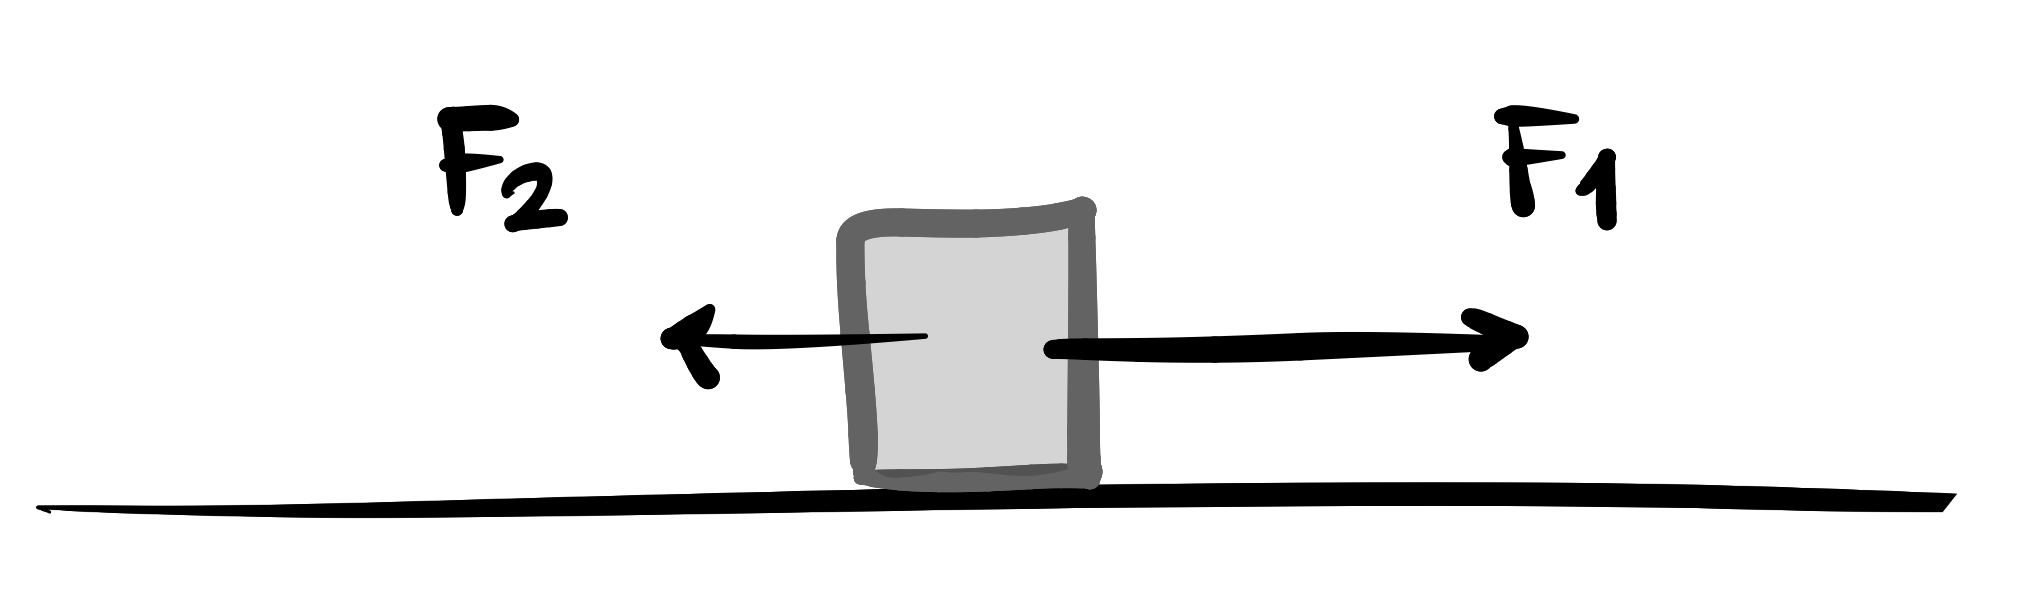
\includegraphics[width=0.4\linewidth]{imagensdinamicanewton/f=ma1.png}};
  \end{scope}
\end{tikzpicture}
\captionof{figure}{Se $F_1 > F_2$, para onde a caixa se move?}
\label{fig_dinamicanewton_f=ma1}
} 
\vspace{0.3cm}

Pelo senso comum, diríamos, com bastante segurança, que a caixa deve se mover para a direita. Razoável, não? Se você pensa assim, por ora, está tudo bem. Uma das mentes mais brilhantes da humanidade também pensava dessa forma -- o filósofo grego Aristóteles. Ocorre que tal conclusão está errada, e é isso que tentaremos perceber juntos a partir de agora.

Note que, ao responder que a caixa se move para a direita, a premissa da qual se parte é que a \textbf{força causa o movimento.} Ou seja, se a força para a direita é maior, então a caixa deve estar se movendo para a direita. Estamos partindo da noção de que existe uma relação de causalidade entre força e movimento. Lembrando que a velocidade é a grandeza física que definimos para medir movimento, estamos dizendo que a força é a causa da velocidade, isto é: a velocidade (ou seja, o movimento) se dá na mesma direção em que a resultante das forças atua:

$$ \boxed{\text{a força é necessária para que haja movimento.} }$$

Logo, se a força resultante for nula, o corpo estaria, segundo este raciocínio, em repouso. A Figura \ref{fig_dinamicanewton_f=ma2} ilustra algumas conclusões tiradas com o uso dessa linha de raciocínio: a caixa sempre se move na direção e no sentido para onde aponta a força resultante.

\vspace{0.3cm}
{
\centering
\begin{tikzpicture}
  \begin{scope}[blend mode=multiply]
    \node {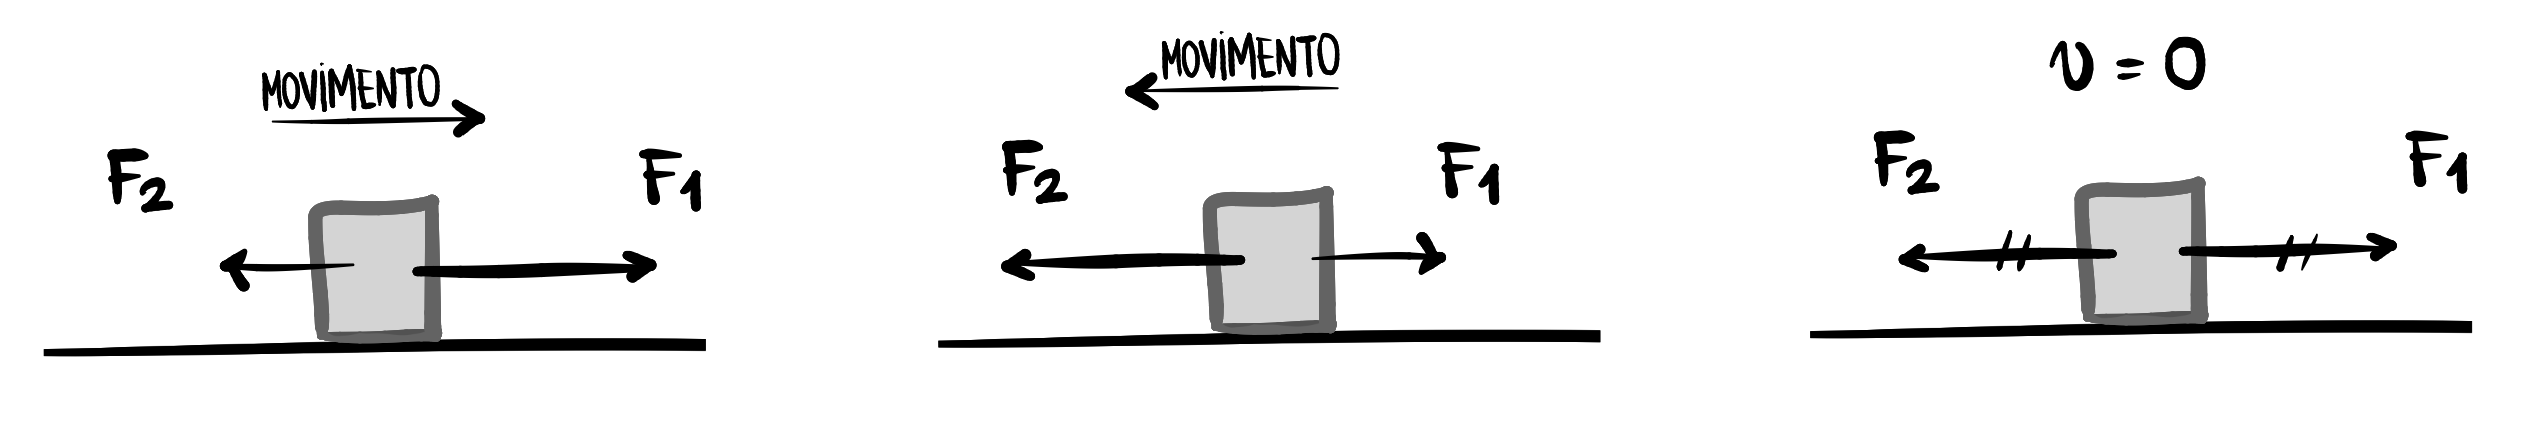
\includegraphics[width=0.9\linewidth]{imagensdinamicanewton/f=ma2.png}};
  \end{scope}
\end{tikzpicture}
\captionof{figure}{Segundo a visão aristotélica de movimento a caixa se moverá no mesmo sentido da força resultante. Se a força total for nula, o movimento (velocidade) da caixa será também nulo.}
\label{fig_dinamicanewton_f=ma2}
} 

\vspace{0.3cm}

Novamente, é importante destacar que tudo que conversamos até aqui é a visão de mundo aristotélica do movimento, e ela está equivocada, como veremos. É claro que tudo isso é bastante intuitivo e parece fazer sentido -- não em vão essa foi a visão de mundo durante quase dois mil anos, até que Galileu e Newton a sobrepujassem com uma nova teoria sobre o movimento. Contudo, se o mundo funcionasse apenas conforme nossa intuição, todo o campo de estudo da Física seria desnecessário. Ocorre que vários fenômenos são bem contraintuitivos e a natureza parece não gostar de funcionar da forma como achamos que ela deveria, e é do estudo dessa natureza aparentemente desobediente que cuida a Física.

Apenas para que o leitor consiga perceber a importância dessa teoria aristotélica do movimento , era a crença nela que incompatibilizou, durante séculos, a teoria de uma terra em movimento. A Figura \ref{fig_dinamicanewton_f=mamovimentoterra} irá nos ajudar a entender como. 

Suponha que a Terra tenha um movimento de rotação em torno do seu próprio eixo. Neste contexto, caso o menino pulasse -- como no ar não haveria nenhuma força que o mantivesse em movimento junto da terra -- ele acabaria ficando para trás, caindo em um ponto diferente do qual ele saltou.\footnote{A título de curiosidade, caso você ficasse por 1 segundo no ar durante este pulo -- o que é factível para um ser humano -- caso o leitor morasse no Pará, exatamente sob a linha do Equador, você ficaria para trás de uns 460 metros em relação ao ponto do qual pulou. Ou seja, com pouco menos de 100 pulos seria possível percorrer a distância do Pará ao Rio Grande do Sul: viajar do norte ao sul do Brasil, em poucos segundos.} Isso é claramente um absurdo e é só você dar um pulo agora onde está para se dar conta de que isso não ocorre.

\vspace{0.3cm}
{
\centering
\begin{tikzpicture}
  \begin{scope}[blend mode=multiply]
    \node {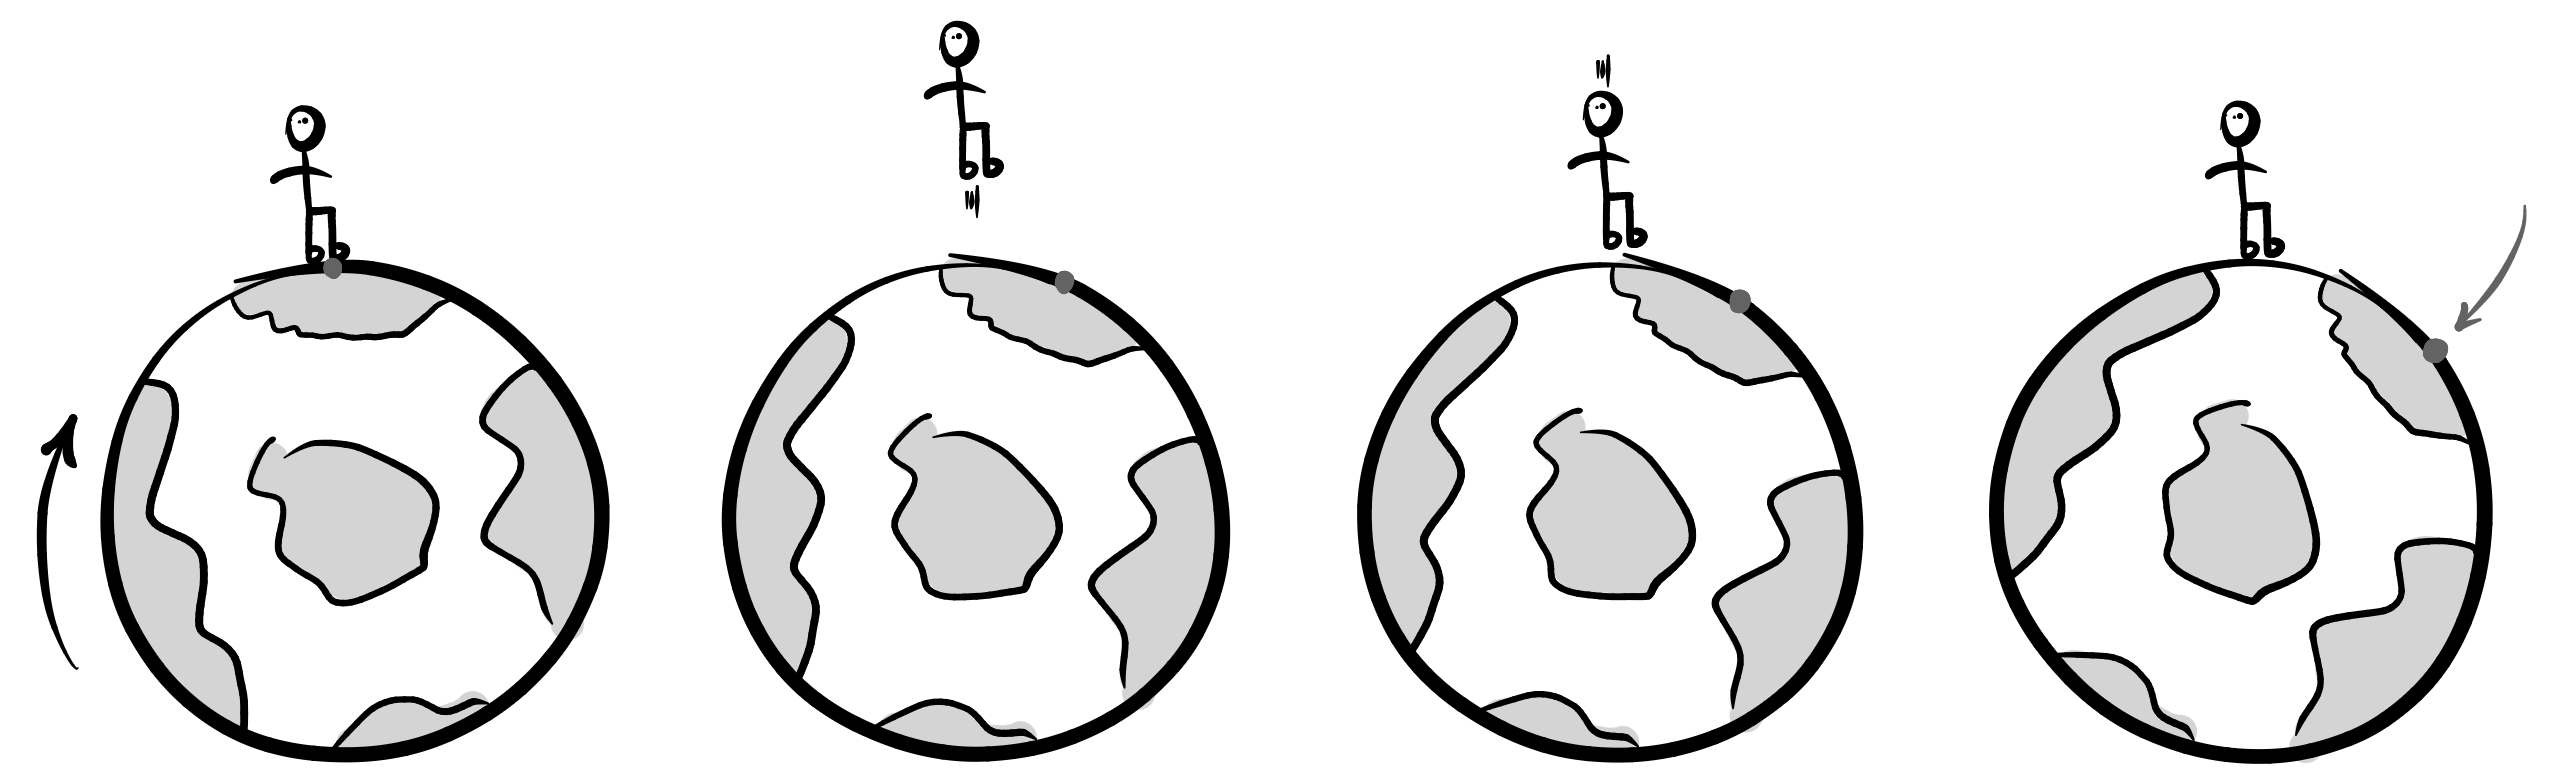
\includegraphics[width=0.8\linewidth]{imagensdinamicanewton/f=ma movimento terra.png}};
  \end{scope}
\end{tikzpicture}
\captionof{figure}{Se a força causa o movimento então uma cosmovisão em que a terra está em movimento é impossível.}
\label{fig_dinamicanewton_f=mamovimentoterra}
} 
\vspace{0.3cm}

O raciocínio, contudo, está impecável, e seguiria a própria lógica aristotélica de silogismos, partindo das premissas $P1,$ $P2$ e $P3,$ a conclusão é natural:

\begin{itemize}
    \item P1: A força causa o movimento.
    \item P2: Se a Terra se movesse, ao pular, no ar, sem contato com ela, não haveria nenhuma força que manteria o menino em movimento junto da Terra.
    \item P3: Logo, o menino iria cair em um ponto diferente daquele em que saltou.
    \item Conclusão: Como isso não ocorre, concluímos que a Terra não se move.
\end{itemize}

É por essas e por outras que levou-se quase dois mil anos para que uma teoria cosmológica em que a Terra estivesse em movimento ganhasse força. Foi apenas no século XVII que algumas teorias, como a de Copérnico, em que o Sol estava no centro e, portanto, a terra em movimento, começaram a se destacar. Isso ocorreu porque uma nova teoria mostrou que a premissa $P1$ estava errada: a força não causa o movimento. Foi Galileu -- um grande defensor do modelo cosmológico de Copérnico -- quem percebeu isso. Vejamos agora como.


Existe um experimento bastante conhecido de Galileu, chamado de experimento dos planos inclinados, que o levou à conclusão de que a força não é necessária para que haja movimento. A Figura \ref{fig_dinamicanewton_f=maplanoinclinado01} ilustra esse experimento: Galileu abandonava do repouso uma bolinha para escorregar ao longo de um plano inclinado, que estava conectado com um outro plano inclinado, todos bastante lisos e bem polidos. \footnote{A importância de deixar o plano bem polido é a de eliminar uma eventual força que pode se manifestar caso o chão não seja perfeitamente liso: a força de atrito. Queremos eliminar essa força justamente porque a intenção é entender o que ocorre com o movimento da bola na \textbf{ausência de forças}. Em breve estudaremos o atrito e entenderemos como ele afeta o movimento.} Ele observava, ao fazer o experimento, que por algum motivo que ele desconhecia a bolinha sempre chegava do outro lado exatamente na mesma altura: nem mais alto, nem mais baixo. 


\vspace{0.3cm}
{
\centering
\begin{tikzpicture}
  \begin{scope}[blend mode=multiply]
    \node {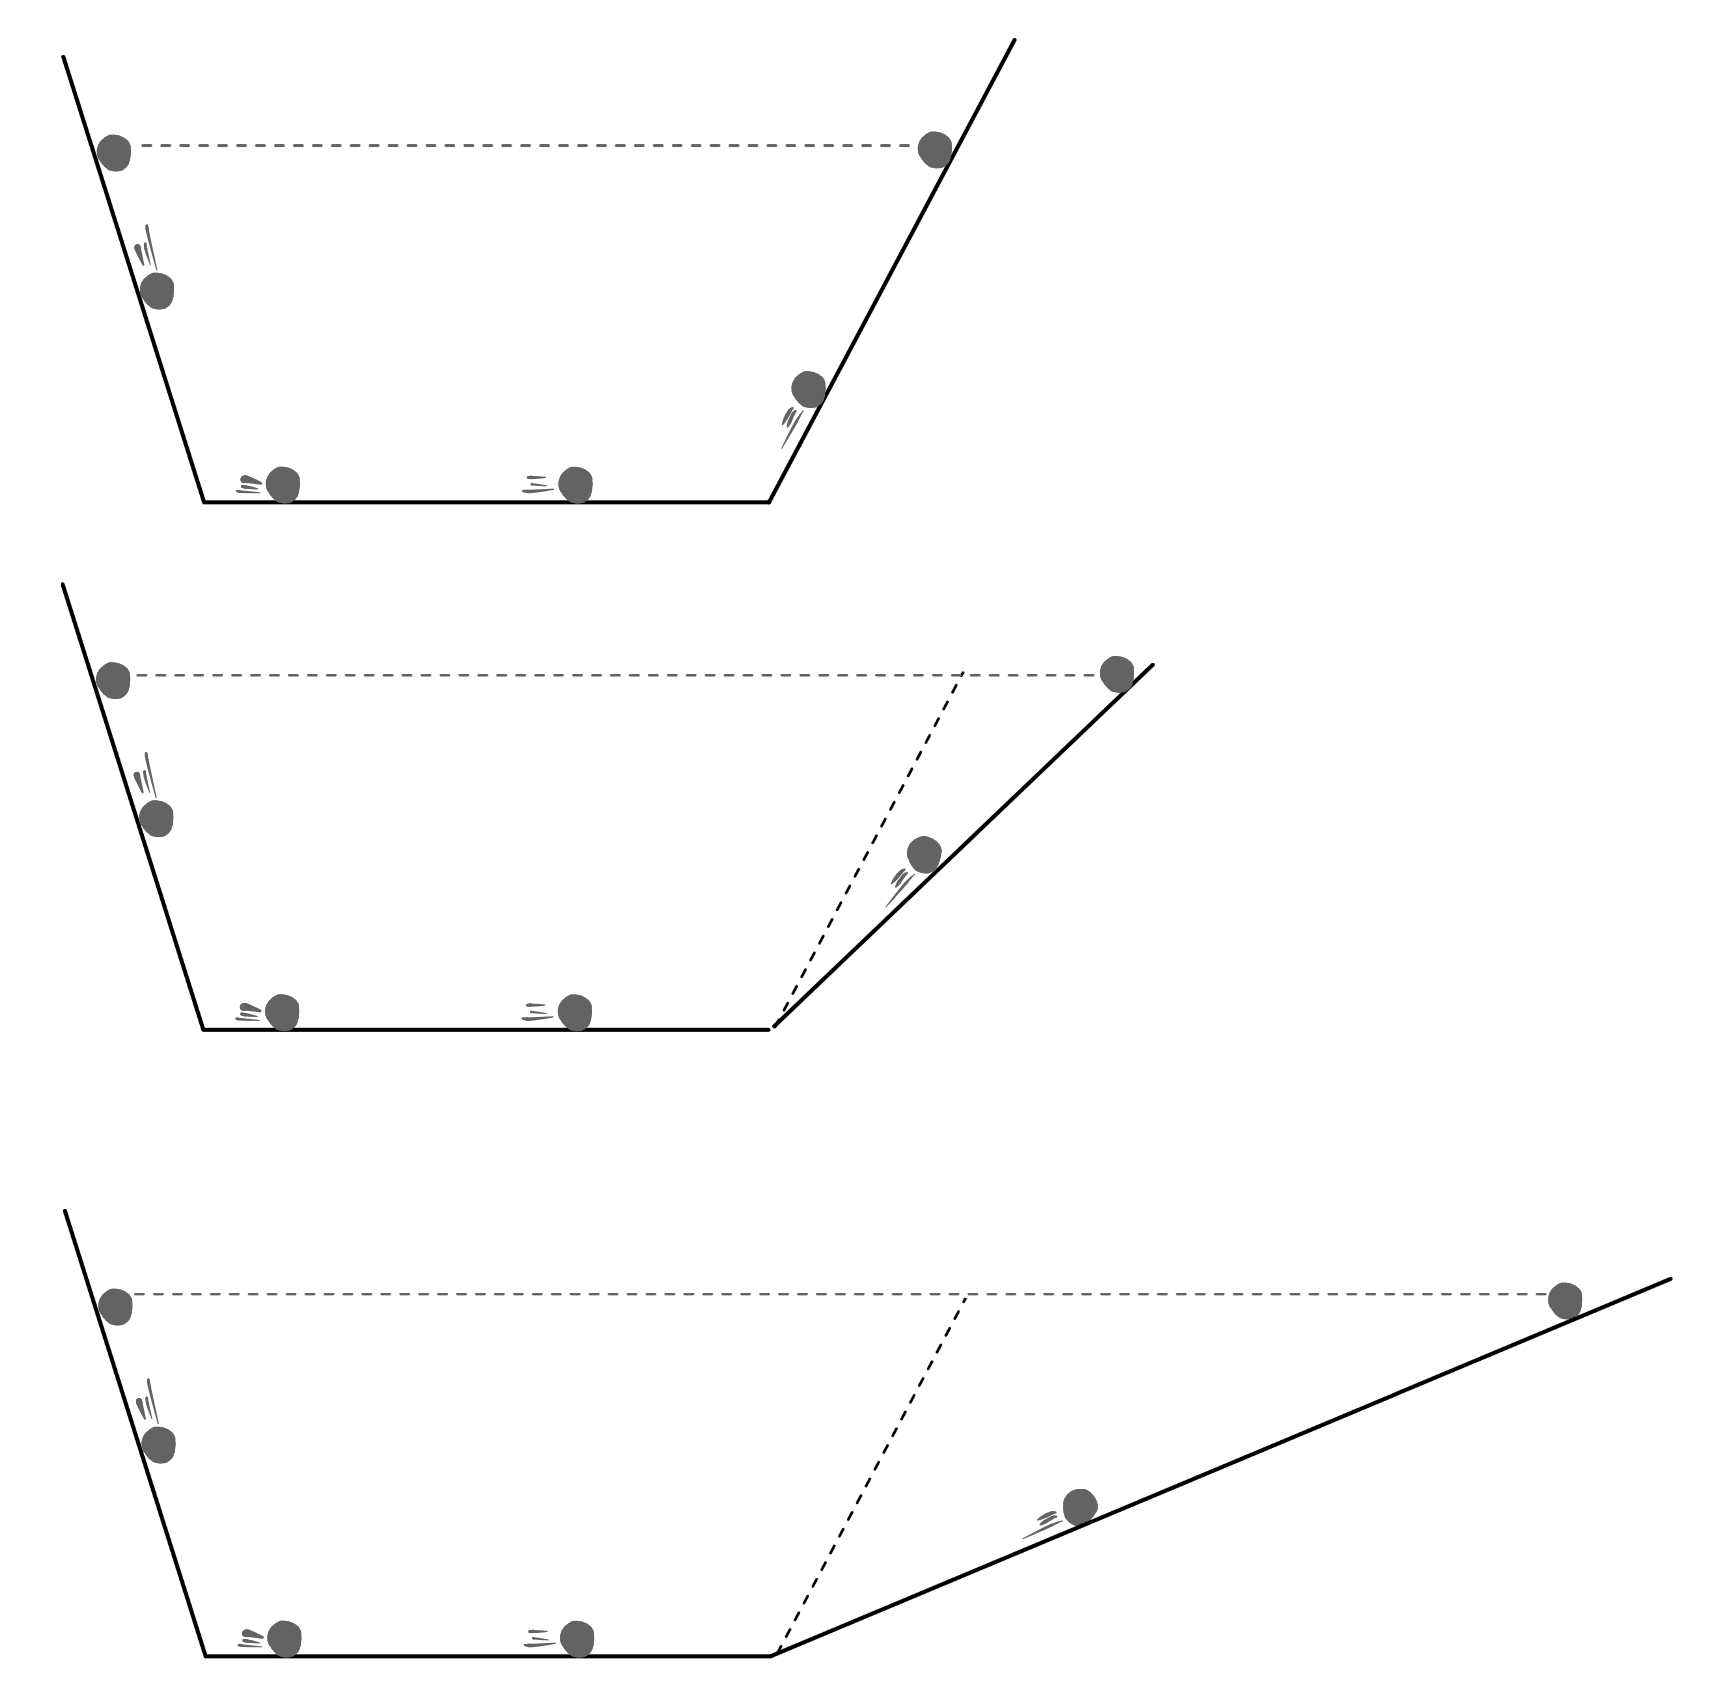
\includegraphics[width=0.6\linewidth]{imagensdinamicanewton/f=ma4.png}};
  \end{scope}
\end{tikzpicture}
\captionof{figure}{Independente da inclinação da rampa a bolinha sempre alcança, do outro lado, a mesma altura.}
\label{fig_dinamicanewton_f=maplanoinclinado01}
} 
\vspace{0.3cm}

Mesmo descendo a inclinação do plano -- o que obrigaria a bolinha a percorrer cada vez mais distância na subida para alcançar a mesma altura -- este era o resultado: a bolinha sempre chegava do outro lado na mesma altura. Partindo da premissa de que essa sempre seria a forma com que a bolinha se comportaria, \footnote{Um estudante mais sabido diria que isso é uma consequência da lei da conservação da energia: a energia potencial $E=mgh$, na descida, se converte em energia cinética, que por sua vez se converte em energia potencial gravitacional de novo na subida da bolinha. Se não existe atrito, o sistema é conservativo e, portanto, a bolinha deve alcançar a mesma altura. Ok, isso faz sentido, mas seria anacrônico usar este raciocínio: na época de Galileu os conceitos de energia cinética, potencial ou de conservação da energia eram inexistentes. Portanto, por mais que ele não soubesse justificar o motivo, era isso que ele observava: as bolinhas sempre chegavam do outro lado na mesma altura. É como se a natureza tivesse uma lei, digamos, ``lei das alturas'', que obrigasse a bolinha a sempre chegar exatamente do outro lado na mesma altura. Galileu estava percebendo como a natureza funcionava, não por que ela funcionava daquela forma -- teorias futuras, como a da conservação da energia, se serviram para dar essa explicação, mas este não é o nosso foco ou interesse neste momento.}, Galileu indaga: \textit{o que aconteceria se deitássemos completamente o plano e reduzíssemos sua inclinação a zero?}

A Figura \ref{fig_dinamicanewton_f=maplanoinclinado02} ilustra a conclusão que o gênio tirou dessa pergunta: como a distância percorrida para chegar à mesma altura aumenta cada vez que deitamos o plano, no caso em que o deitarmos completamente, a distância que a bolinha teria que percorrer seria infinita: ela permaneceria se movendo, com a mesma velocidade, até o infinito. \footnote{Caso o leitor já tenha escutado que retas paralelas se encontram no infinito, perceba, pela imagem da Figura \ref{fig_dinamicanewton_f=maplanoinclinado02}, que, para que a bolinha retorne à mesma altura, a linha cheia, que representa o plano horizontal, teria que encontrar a linha pontilhada, que representa o mesmo nível de altura em que a bolinha foi abandonada. Assim, sendo essas linhas paralelas, a bolinha teria que ir até o infinito para chegar à mesma altura. Não espere que o leitor acredite que o autor tenha ido pessoalmente ao infinito para observar o suposto encontro das paralelas. Tal expedição, além de custosa, parece logisticamente complexa. Recebeu tal informação de um amigo -- sujeito de boa índole e de caráter sólido -- mas, como se vê, trata-se de um testemunho indireto. Quanto à comprovação empírica, resta-lhe a humildade de admitir que não a possui.} Tal movimento se daria sem a necessidade de ter qualquer força para manter a bolinha em movimento: o movimento se perpetuaria, de modo natural, na ausência de forças. Trata-se de um movimento bem especial, como a Figura \ref{fig_dinamicanewton_f=maplanoinclinado02} ilustra: o Movimento Uniforme em Linha Reta, como descrito por Isaac Newton, ou o Movimento Retilíneo Uniforme (MRU), como descrito atualmente nos almanaques de ensino de Física. É um movimento, em linha reta, com velocidade constante. 

Perceba que isso contraria a visão aristotélica de movimento: estamos falando de um movimento que se perpetua na ausência de forças, ou seja, \textbf{não é preciso nenhuma força para manter a bolinha neste movimento, o MRU.} A isso, futuramente, Isaac Newton deu o nome de inércia: a capacidade que um corpo tem de permanecer no seu estado de movimento. Ou seja, podemos dizer que a bolinha \textit{se move por inércia}: ela não precisa de nenhuma força para se manter em movimento; ela se move porque é assim que a natureza funciona -- corpos em movimento tendem a permanecer no seu estado de movimento, não é necessária força para mantê-los em movimento. A força é necessária apenas para alterar o seu estado de movimento.

\vspace{0.3cm}
{
\centering
\begin{tikzpicture}
  \begin{scope}[blend mode=multiply]
    \node {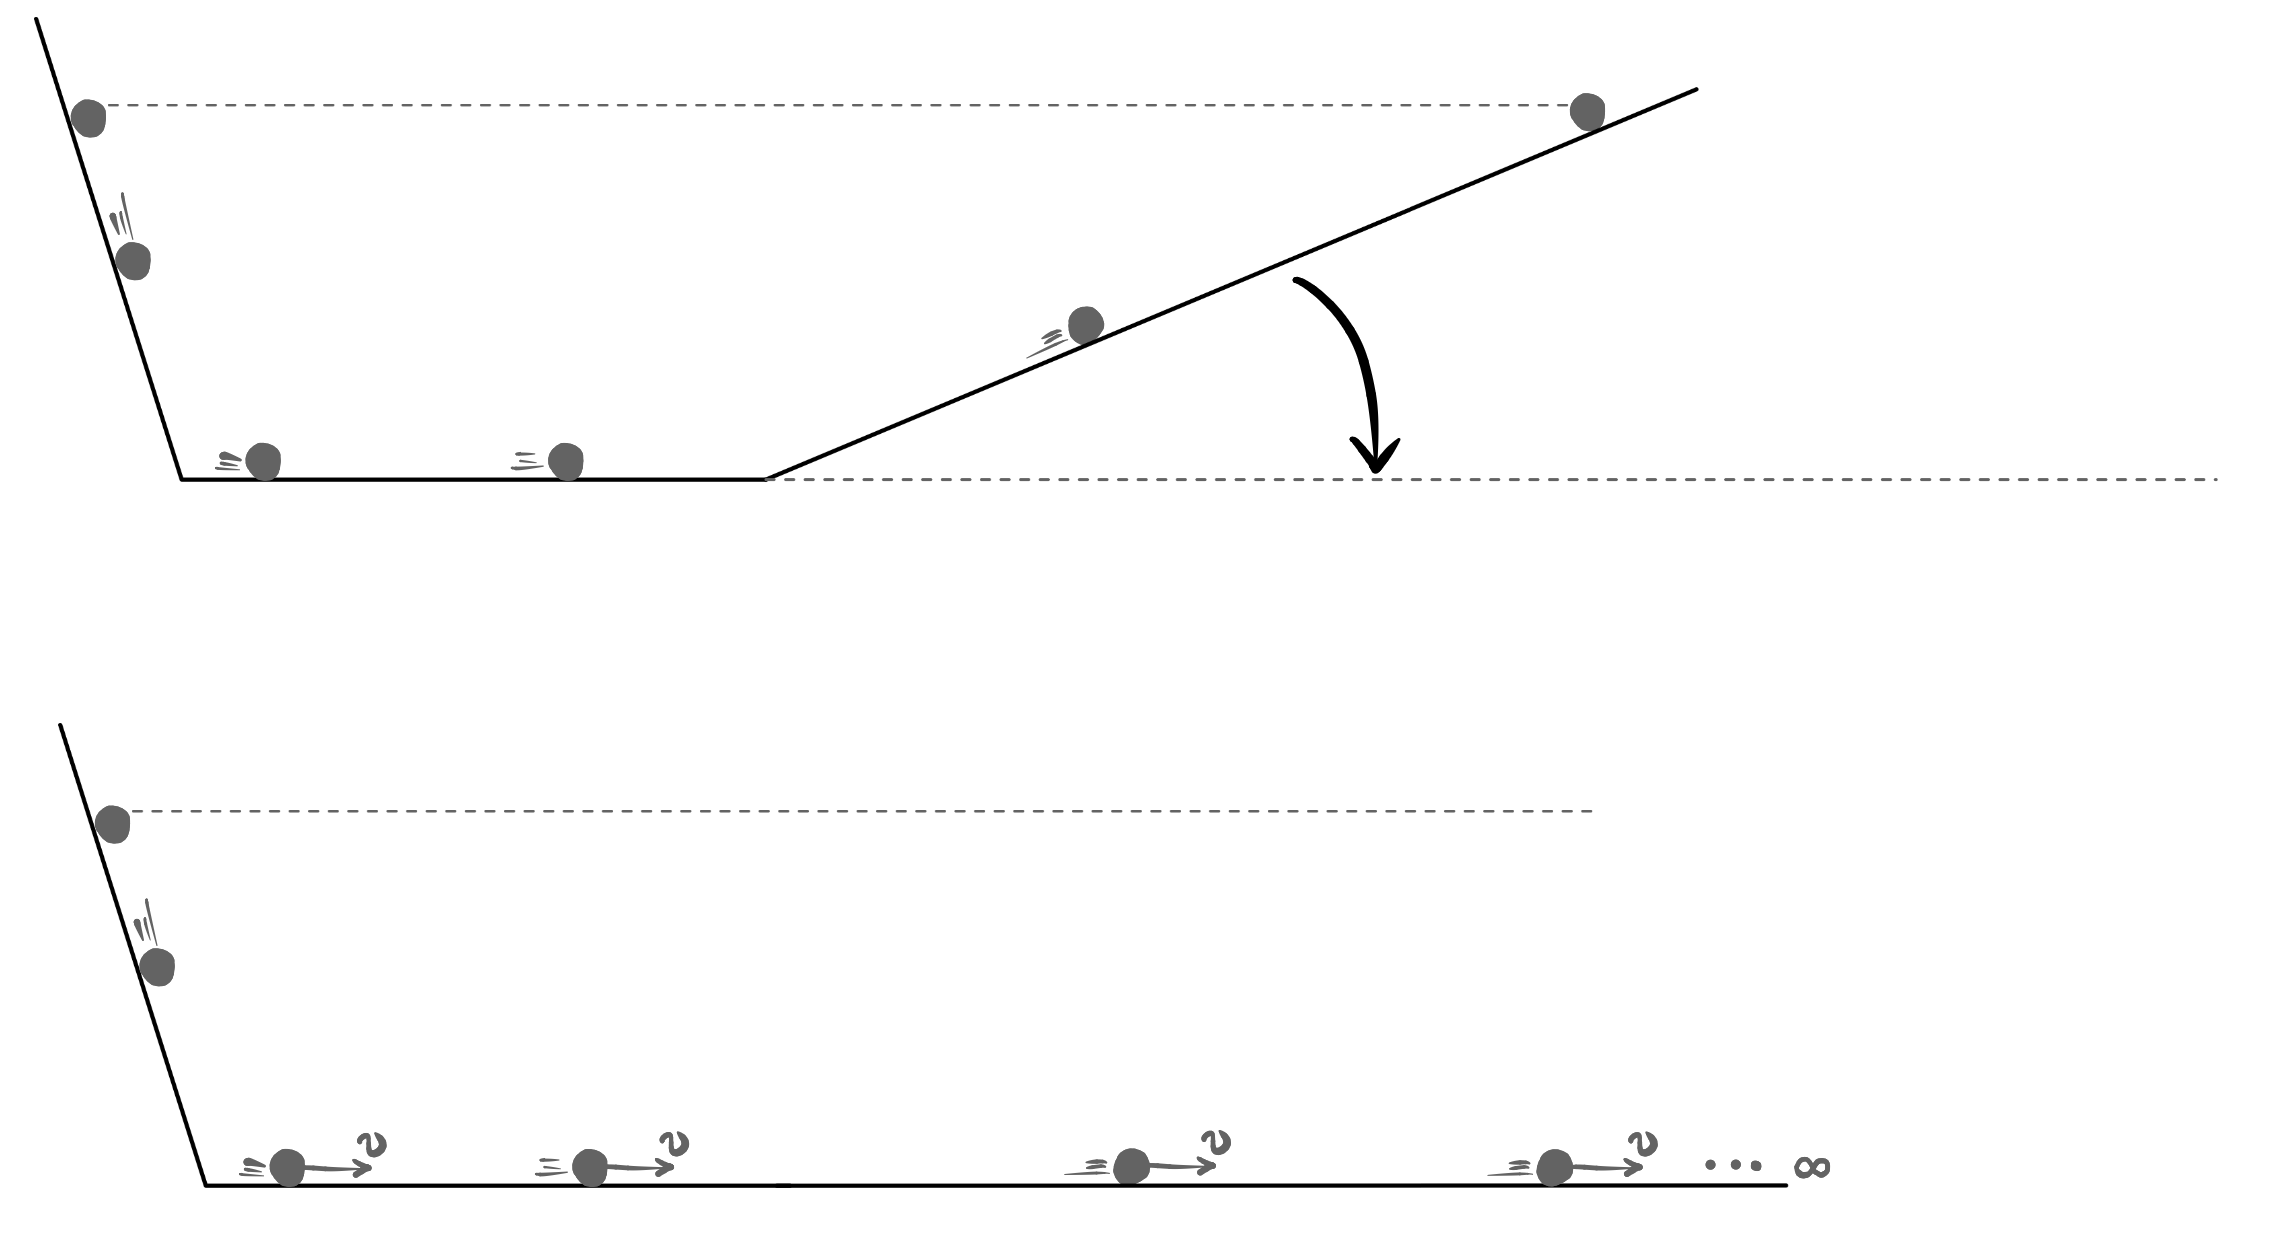
\includegraphics[width=0.8\linewidth]{imagensdinamicanewton/f=ma5.png}};
  \end{scope}
\end{tikzpicture}
\captionof{figure}{Ao reduzir a inclinação do plano a zero a bolinha teria que percorrer uma distância infinita para chegar à mesma altura.}
\label{fig_dinamicanewton_f=maplanoinclinado02}
} 

\vspace{0.3cm}



Os experimentos das três imagens da Figura \ref{fig_dinamicanewton_f=maplanoinclinado01} poderiam e foram, de fato, executados por Galileu. Já o experimento da segunda imagem da Figura \ref{fig_dinamicanewton_f=maplanoinclinado02} não foi executado por ele -- e sequer poderia sê-lo. Primeiro porque ele não tinha material infinito para produzir um plano de tamanho infinito. Mesmo que o tivesse, levaria um tempo infinito para observar a bolinha se movendo, bem, até o infinito. 

Logo, existe de fato um salto aqui -- um salto que, talvez, apenas um gênio conseguiria dar sozinho. O último experimento não foi realizado e, como visto, sequer poderia sê-lo. Foi uma conclusão tirada a respeito de como a coisa toda deveria funcionar em um caso que seria teórico, ideal e irrealizável na prática; partindo do entendimento tirado dos experimentos que eram de fato realizáveis. Galileu visualiza a estrutura com que a natureza parece funcionar, entende o que ela quer lhe comunicar e, finalmente, extrapola para o campo da abstração e tira a conclusão do caso que seria impossível de se realizar ou observar: na ausência perfeita de atrito, ao deitar completamente o plano, a bolinha teria que se mover indefinidamente, com a mesma velocidade, até o infinito. Logo, não se precisa de força alguma para mantê-la em movimento e, portanto, a força deixa de ser necessária para que haja movimento. Pronto: desconstruiu-se quase 2 mil anos de pensamento e uma nova ideia sobre o movimento começa a surgir.

A força, agora, é entendida como necessária para \textbf{alterar o movimento}:  se a bolinha está parada, é necessária uma força para colocá-la em movimento. Se ela está em movimento, é necessária alguma força para fazê-la andar mais depressa ou mais devagar -- mas não é preciso força para mantê-la em movimento:

$$ \boxed{\text{a força é necessária para que haja \textbf{variação} do movimento.} }$$

Se o leitor tentar realizar o experimento da Figura \ref{fig_dinamicanewton_f=maplanoinclinado02} vai perceber que a bolinha, diferente do que dissemos, não se move até o infinito. Ela, na verdade, se moverá por alguns metros ao longo do plano horizontal e irá parar logo depois. Isso ocorre porque é impossível ter uma superfície perfeitamente polida: por mais que se lixe ou lubrifique o material para tentar deixá-lo o mais liso possível, a fim de eliminar o atrito, isso nunca pode ser feito de forma perfeita, de modo que o atrito estará sempre presente, por menor que ele seja. 

Assim, sendo a força de atrito, neste caso, uma força que se opõe ao movimento e, como a força causa a variação do movimento, ela irá variar o movimento, diminuindo-o até ele cessar. Ou seja, a força aqui retarda a bolinha, fazendo-a parar -- e é por isso que, no experimento real, ela não vai até o infinito. Mais uma vez, é necessária a capacidade de pensar de forma abstrata para concluir o que Galileu conclui: é uma experiência de pensamento, feita na nossa cabeça, em um mundo ideal, e nos serve para entender, na sua essência mais pura, como o movimento funciona.

Perceba que a diferença entre a perspectiva Galileana/Newtoniana \footnote{Aqui não nos atemos a explicar muito essa diferença entre Galileu e Newton, mas ocorre que Galileu foi o primeiro a perceber essas ideias, mas não conseguiu unificá-las e estruturá-las em uma nova teoria completa a respeito do movimento, capaz de substituir a teoria aristotélica. Isso foi feito posteriormente por Isaac Newton.} em relação à Aristotélica é sutil: a visão aristotélica do movimento entendia que a força $F$ era necessária para que houvesse movimento, ou seja, sendo a velocidade $v$ a grandeza física que mede o movimento, teríamos que

$$ F \propto v,$$

\noindent ou seja, a força seria proporcional à velocidade, pensando em termos mais matemáticos. Já na visão Galileana/Newtoniana a força $F$ era necessária para que houvesse \textbf{variação} do movimento, ou seja, sendo a aceleração $a$ a grandeza física que mede o a variação do movimento, isto é, a variação da velocidade, teríamos que

$$ F \propto a,$$

\noindent ou seja, a força seria proporcional à aceleração, e não à velocidade.

Da relação de proporção direta acima para desaguarmos na Equação \eqref{eq_dinamica1_segundaleinewton} falta apenas um passo: adicionar a massa $m$ como constante de proporcionalidade e, voilà, temos a Segunda Lei de Newton: $F = ma.$ Em breve discutiremos a razão da massa ser a constante de proporcionalidade. Por ora, vamos nos atentar à sutil mudança de que agora a força é necessária para causar a variação do movimento, e não o movimento em si.


Note que, nessa nova perspectiva, o problema da Figura \ref{fig_dinamicanewton_f=ma1} não faria sentido: não tem como saber para onde o bloco se move só sabendo das forças, uma vez que agora a força não tem relação direta com o movimento, mas sim com a variação dele. Ainda no contexto de tal figura, em que $F_1 > F_2,$ isto é, a força resultante aponta para a direita, o bloco poderia ter diferentes velocidades, como ilustra a Figura \ref{fig_dinamicanewton_f=ma3}. O bloco poderia estar


\begin{enumerate}
    \item [(i)] se movendo para a direita -- ocasião em que o movimento seria acelerado, uma vez que a força resultante estaria a favor da velocidade, aumentando o movimento (aumentando a velocidade);
    \item [(ii)] se movendo para a esquerda -- ocasião na qual o movimento seria retardado, uma vez que a força resultante estaria no sentido contrário ao da velocidade, diminuindo o movimento (a velocidade);
    \item [(iii)] em repouso instantâneo, ou seja, $v=0$ -- ocasião na qual certamente o bloco começaria a se mover para a direita, uma vez que, sendo a força responsável por variar o movimento, estando ela para a direita, com o bloco em repouso, ela alteraria este estado de movimento (repouso) fazendo com que o bloco começasse a se mover na direção e sentido para a qual a força resultante aponta.
    
\end{enumerate}



{
\centering
\begin{tikzpicture}
  \begin{scope}[blend mode=multiply]
    \node {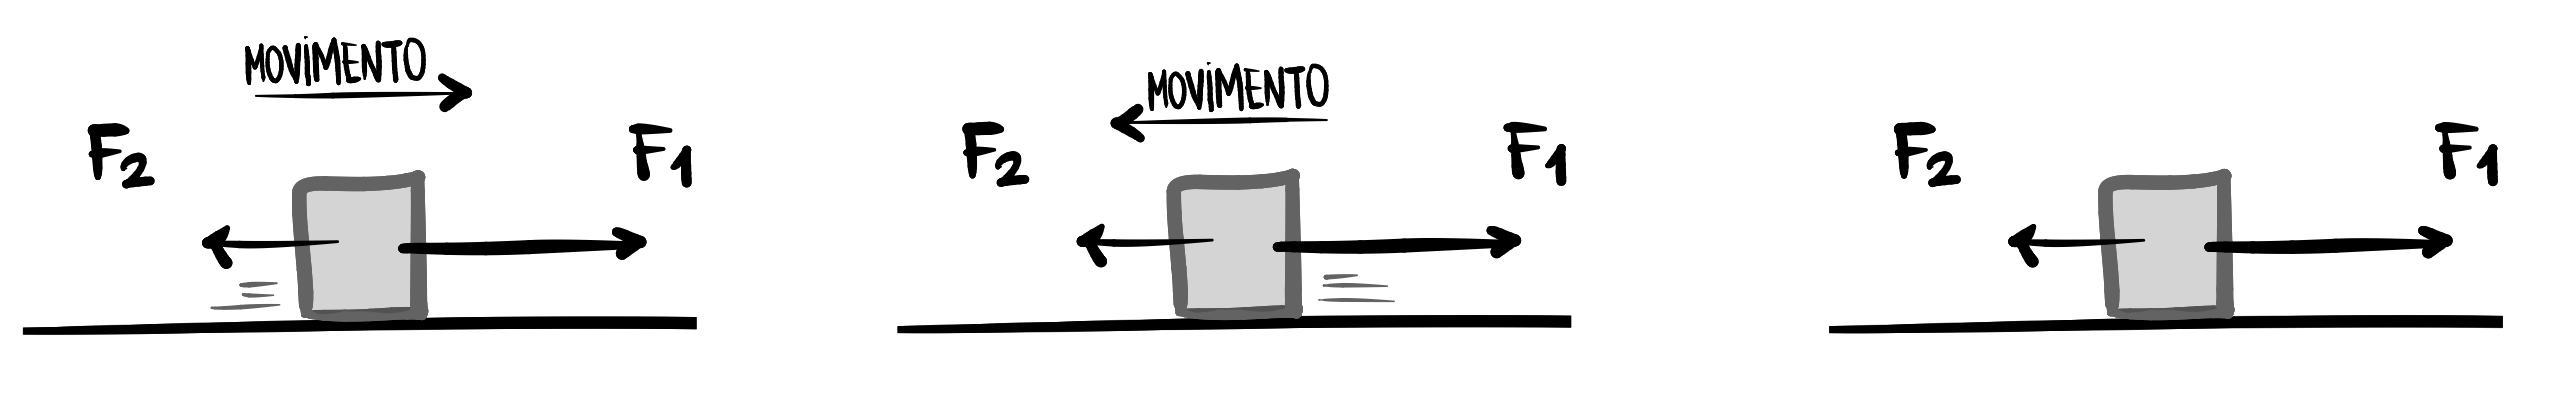
\includegraphics[width=0.8\linewidth]{imagensdinamicanewton/f=ma3.png}};
  \end{scope}
\end{tikzpicture}
\captionof{figure}{Tendo a força resultante para direita, o bloco pode ter qualquer tipo de velocidade, uma vez que a força não causa o movimento (velocidade) mas sim a sua variação (aceleração).}
\label{fig_dinamicanewton_f=ma3}
} 

\vspace{0.3cm}

Portanto, ao te fornecer a situação da Figura \ref{fig_dinamicanewton_f=ma1} e te perguntar para onde o bloco se move, tal pergunta deixa de fazer sentido no paradigma galileano/newtoniano, uma vez que, com forças, podemos determinar apenas como será a variação do movimento, e não o movimento em si. Como a \textbf{força causa a variação do movimento}, precisaríamos de, pelo menos, dois instantes distintos para tirar quaisquer conclusões, percebendo como o movimento varia de um instante para o outro.

\vspace{0.3cm}
{
\centering
\begin{tikzpicture}
  \begin{scope}[blend mode=multiply]
    \node {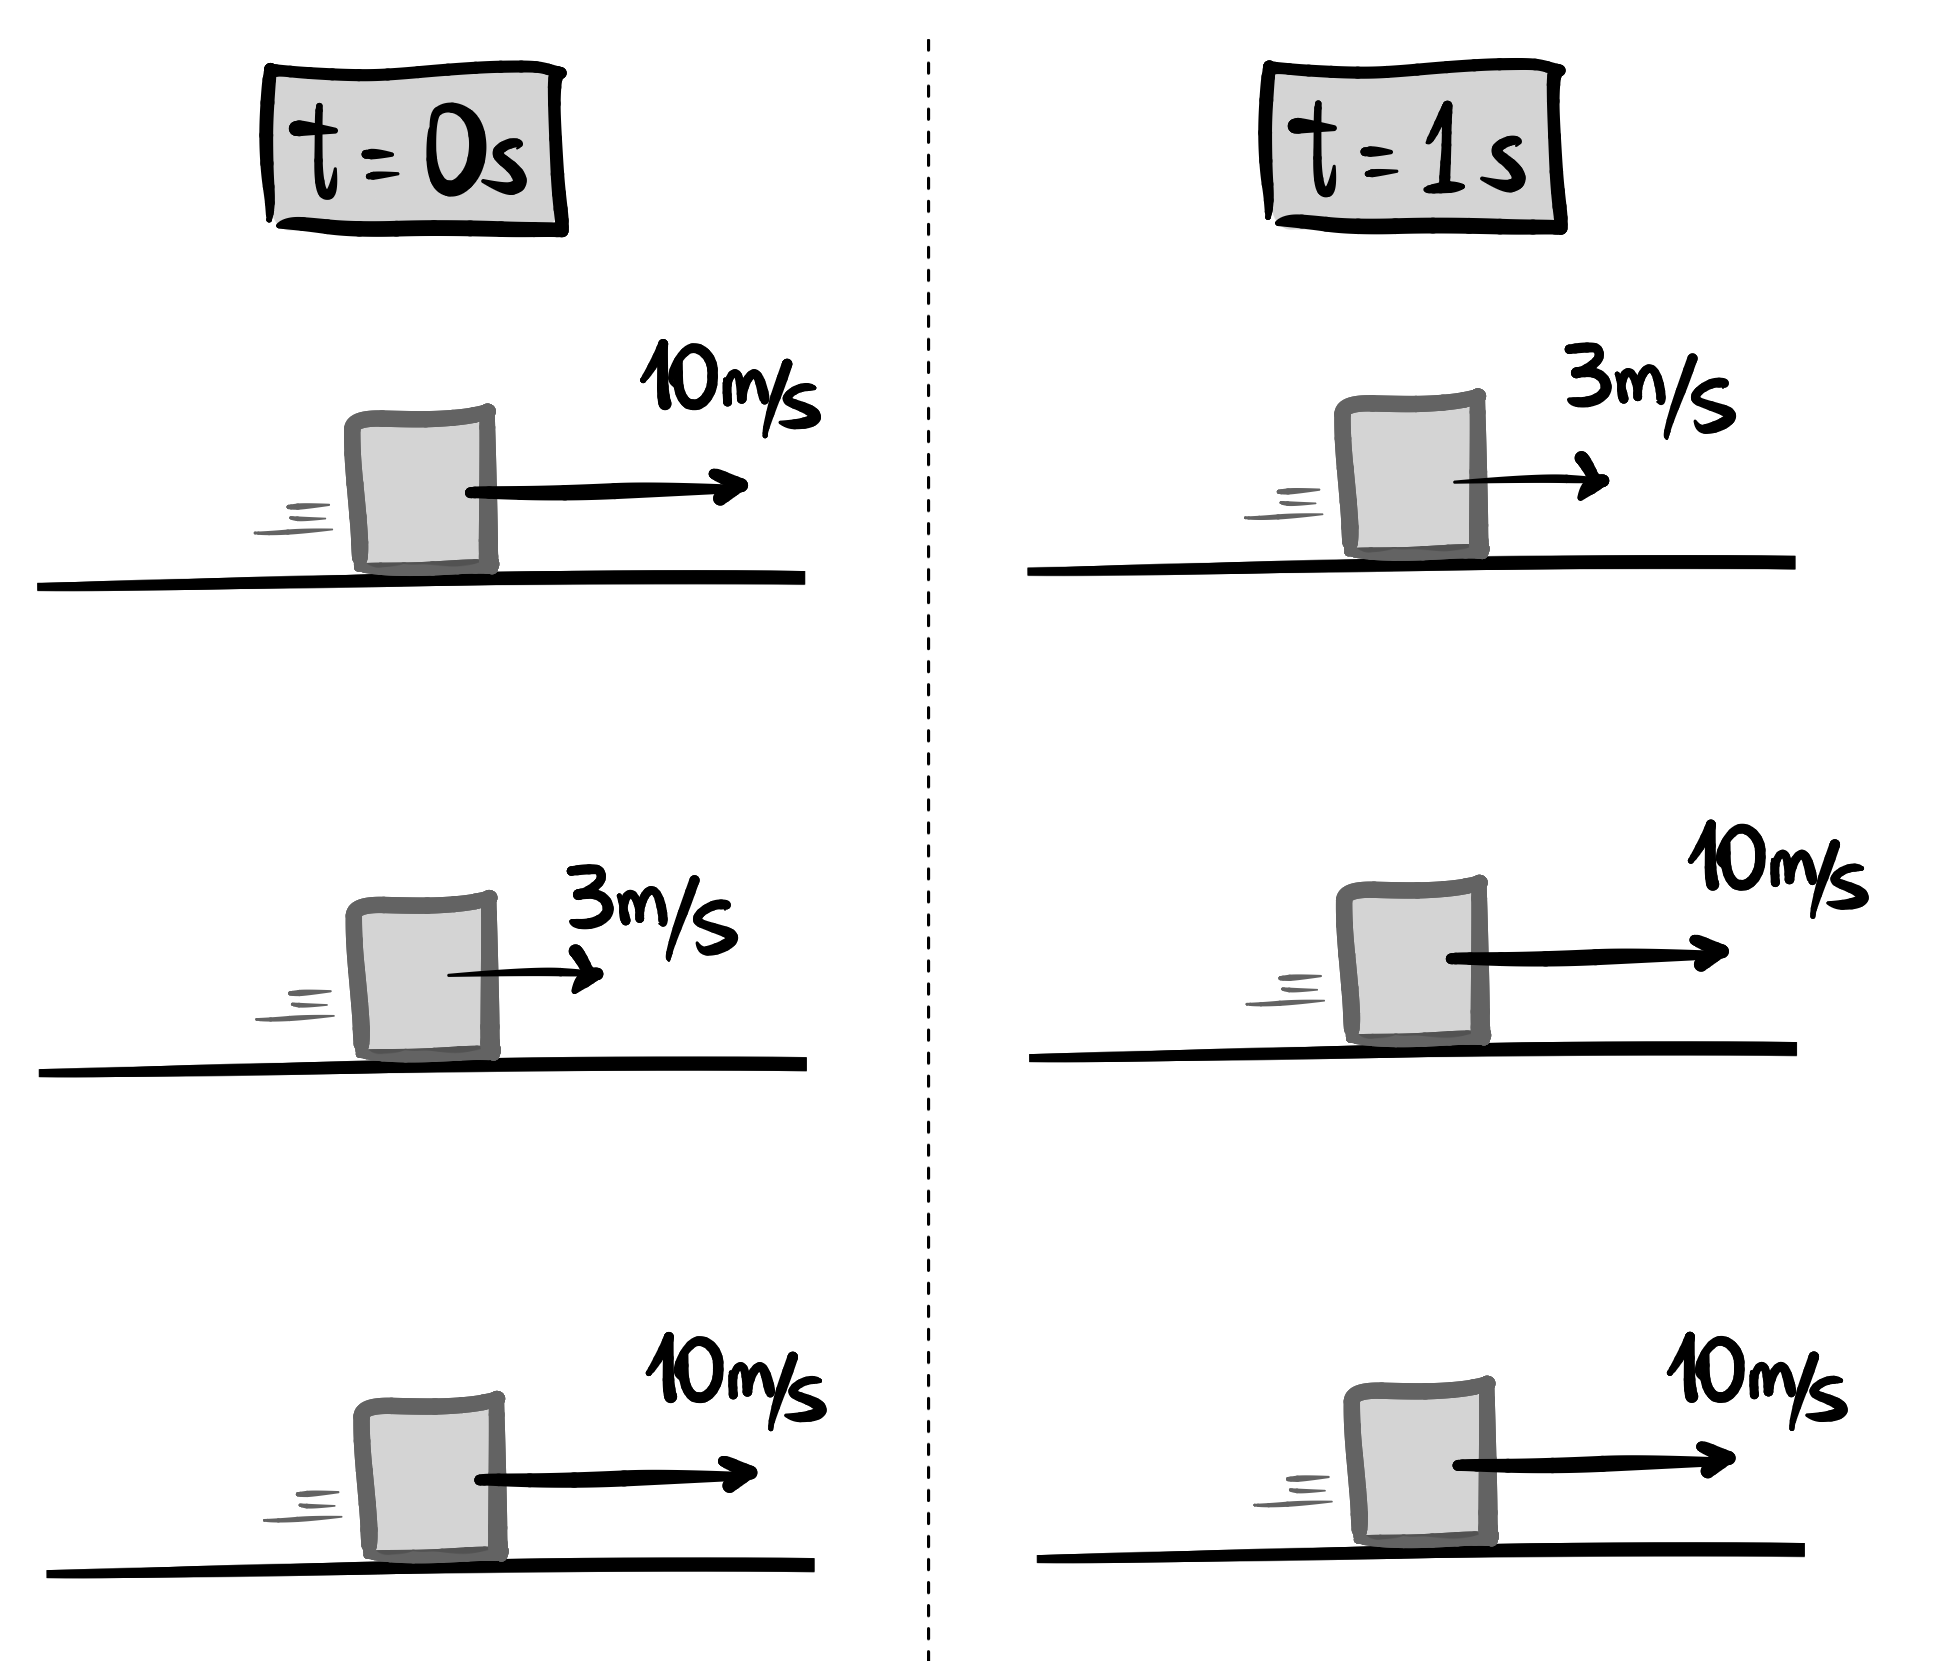
\includegraphics[width=0.4\linewidth]{imagensdinamicanewton/f=ma variacao movimento.png}};
  \end{scope}
\end{tikzpicture}
\captionof{figure}{Para obter informação sobre a força é preciso saber se houve variação do movimento (aceleração).}
\label{fig_dinamicanewton_f=ma variacao movimento}
} 
\vspace{0.3cm}

Essa é a situação da Figura \ref{fig_dinamicanewton_f=ma variacao movimento}, que mostra dois instantes distintos de um mesmo movimento. Ao avaliar o que ocorreu com o movimento (velocidade) de um instante para o outro, podemos concluir sobre a força que eventualmente atua no corpo. Avaliemos cada situação:

\begin{enumerate}
    \item [(i)] Na primeira linha, vemos que o movimento (velocidade) diminuiu de $t=0s$ para $t=1s$. Como houve variação do movimento, deve ter tido algum tipo de força para gerá-lo. Como o movimento (velocidade) diminuiu, concluímos que havia uma força contrária ao movimento, empurrando o bloco para a esquerda e gerando uma desaceleração nele.


    \item [(ii)] Na segunda linha, vemos que o movimento (velocidade) aumentou. Ora, se há variação do movimento, deve ter tido algum tipo de força para gerá-lo. Como o movimento (velocidade) aumentou, concluímos que havia uma força favorável ao movimento, empurrando o bloco para a direita e gerando uma aceleração nesse sentido.
     
    \item [(iii)] Na terceira linha percebemos que não houve variação no movimento de $t=0s$ para $t=1s$. Assim, concluímos que $F_R=0,$ isto é, se houver quaisquer tipos de forças atuando no bloco, elas devem se anular.\footnote{Vale destacar, correndo o risco de ser repetitivo: a condição $F_\text{R}=0$ não quer dizer que não há forças atuando no corpo. Podem sim haver forças, mas elas devem se anular.} Esse seria justamente o caso do MRU: o corpo tende a permanecer no seu estado de movimento, sem precisar de nenhum tipo de força para fazê-lo. A isso damos o nome de inércia.
\end{enumerate}


Acredito que já está mais do que clara a diferença entre a noção aristotélica e a noção galileana/newtoniana de movimento. Galileu foi o primeiro que começou a entender que não era preciso força para manter um corpo em movimento, mas foi Newton -- que nasceu em 1642, no mesmo ano em que Galileu morreu -- quem sintetizou e estruturou tudo isso.\footnote{ Inclusive, esse foi um dos erros cometidos por Galileu: para ele, a ideia de inércia não era restrita ao movimento retilíneo; ele admitia que podia haver uma espécie de \emph{inércia circular} em certos contextos. A definição completa e correta de inércia só viria com Newton.} A essa altura, é importante que o leitor perceba como a Equação \eqref{eq_dinamica1_segundaleinewton} condensa tudo o que conversamos até aqui: as conclusões do experimento dos planos inclinados estão capturadas ali; a ruptura com a física aristotélica está ali; a possibilidade de movimento na ausência de forças está ali. O que antes ocupava páginas de argumentação e descrição experimental agora repousa elegantemente em poucos símbolos.

Este é o verdadeiro poder de uma equação matemática: não apenas representar, mas sintetizar. Ela é capaz de comprimir uma longa sequência de raciocínios, experimentos e mudanças conceituais em uma expressão compacta. A Equação \eqref{eq_dinamica1_segundaleinewton} não inaugura a discussão — ela a encerra. Não é o ponto de partida do pensamento, mas o seu ponto de chegada: é nela que toda essa nossa longa conversa se organiza, se depura e se transforma em forma matemática.

Para perceber como tal equação contém a informação de que é possível a existência de movimento na ausência de força -- a grande ruptura com o paradigma aristotélico -- basta avaliar o que ela nos diz na ausência de forças, isto é, quando $F_R=0$:

$$ \vec F_R = m \vec a \xrightarrow{ \text{ } F_R = 0 \text{ } } \cancelto{0}{  \vec F_R }= m \cancelto{0}{  \vec a }  \xrightarrow{\text{  }} \vec a  =  0 \xrightarrow{ \text{ como } \vec a = \sfrac{\Delta \vec v}{\Delta t} \text{ }} \vec v \text{ é constante},  $$

\noindent ora, mas se o vetor velocidade $\vec v$ é constante, só há duas opções:

\begin{enumerate}
    \item [(i)] $\vec v = 0$, isto é, a partícula está em repouso. Este caso é simples e já estava dentro da visão de mundo aristotélica: na ausência de forças, um corpo deve necessariamente ficar em repouso, haja vista que o movimento, para Aristóteles, só pode se manter por meio da aplicação de forças.

    \item[(ii)] $\vec v$ é constante e diferente de zero. Por ser um vetor, para que ele seja constante é preciso que
       \begin{enumerate}
           \item Sua direção e sentido seja constante. Logo, o movimento deve ser \textbf{retilíneo}, uma vez que fazer curvas implica em mudar a direção do vetor velocidade.

           \item Seu valor (módulo) deve ser constante: o corpo não pode se mover mais rápido nem mais devagar, mas sempre na mesma velocidade. Ou seja, o movimento deve ser \textbf{uniforme.}
       \end{enumerate}

       Esta é a grande novidade na perspectiva Newton/Galileu: na ausência de forças, além do repouso, existe também um outro estado de movimento possível: o MRU. Aqui fica claro porque ele é tão especial: ele é o único movimento em que o vetor velocidade é constante em todas as suas características: a velocidade não muda em direção nem sentido (daí a necessidade de ser retilíneo) nem em valor (por isso o movimento é uniforme).
\end{enumerate}

Assim, a própria Equação \eqref{eq_dinamica1_segundaleinewton} contêm os dois possíveis estados de movimentos inerciais, ou seja, estados de movimento que ocorrem na ausência de forças: repouso \footnote{Talvez o leitor possa achar isso estranho, mas é comum nos referirmos ao repouso como um estado de movimento.} e MRU.


Estando claro a origem, história e significado da Equação  \eqref{eq_dinamica1_segundaleinewton}, resta-nos entender por que a massa $m$ é a constante de proporcionalidade que aparece ali. Tentarei ser breve nesta justificativa, para não correr o risco de me alongar mais do que o necessário -- mas certas equações, sobretudo esta, não se deixam atravessar com pressa. Sendo talvez a mais importante de toda a Física escolar, ela merece, sem dúvida, algum gasto adicional de palavras e de calorias do pensamento.

Indo direto ao ponto, o motivo principal da massa $m$ aparecer na Equação \eqref{eq_dinamica1_segundaleinewton} é porque a \textbf{massa é uma medida da inércia}, isto é, da capacidade que um corpo tem de permanecer em seu estado de movimento. Considere, por exemplo, um caminhão, inicialmente parado. Ao tentar empurrá-lo, ou seja, exercer uma força $F$, a fim de alterar seu estado de movimento -- colocá-lo em movimento -- o leitor há de encontrar certa dificuldade nessa tarefa. Isso porque, tendo o caminhão uma grande massa $m,$ sua inércia é muito alta: é difícil alterar o seu estado de movimento.

O mesmo valeria caso o caminhão estivesse se movendo a uma certa velocidade constante: é preciso muita força para pará-lo: sua inércia (tendência de permanecer no seu atual estado de movimento) é elevada, o que exige uma força maior para alterar seu estado de movimento.

Já um corpo de pouca massa, como uma bola de futebol, pode ter seu estado de movimento facilmente alterado com a aplicação de uma pequena força. Estando ela parada, com o chute de uma criança, conseguimos romper seu repouso e colocá-la em movimento. Estando ela em movimento, basta, talvez, o corpo de uma outra criança para interceptá-la e colocá-la em repouso: a inércia (massa) da bola é baixa, é preciso pouca força para alterar seu estado de movimento.

\vspace{0.3cm}
{
\centering
\begin{tikzpicture}
  \begin{scope}[blend mode=multiply]
    \node {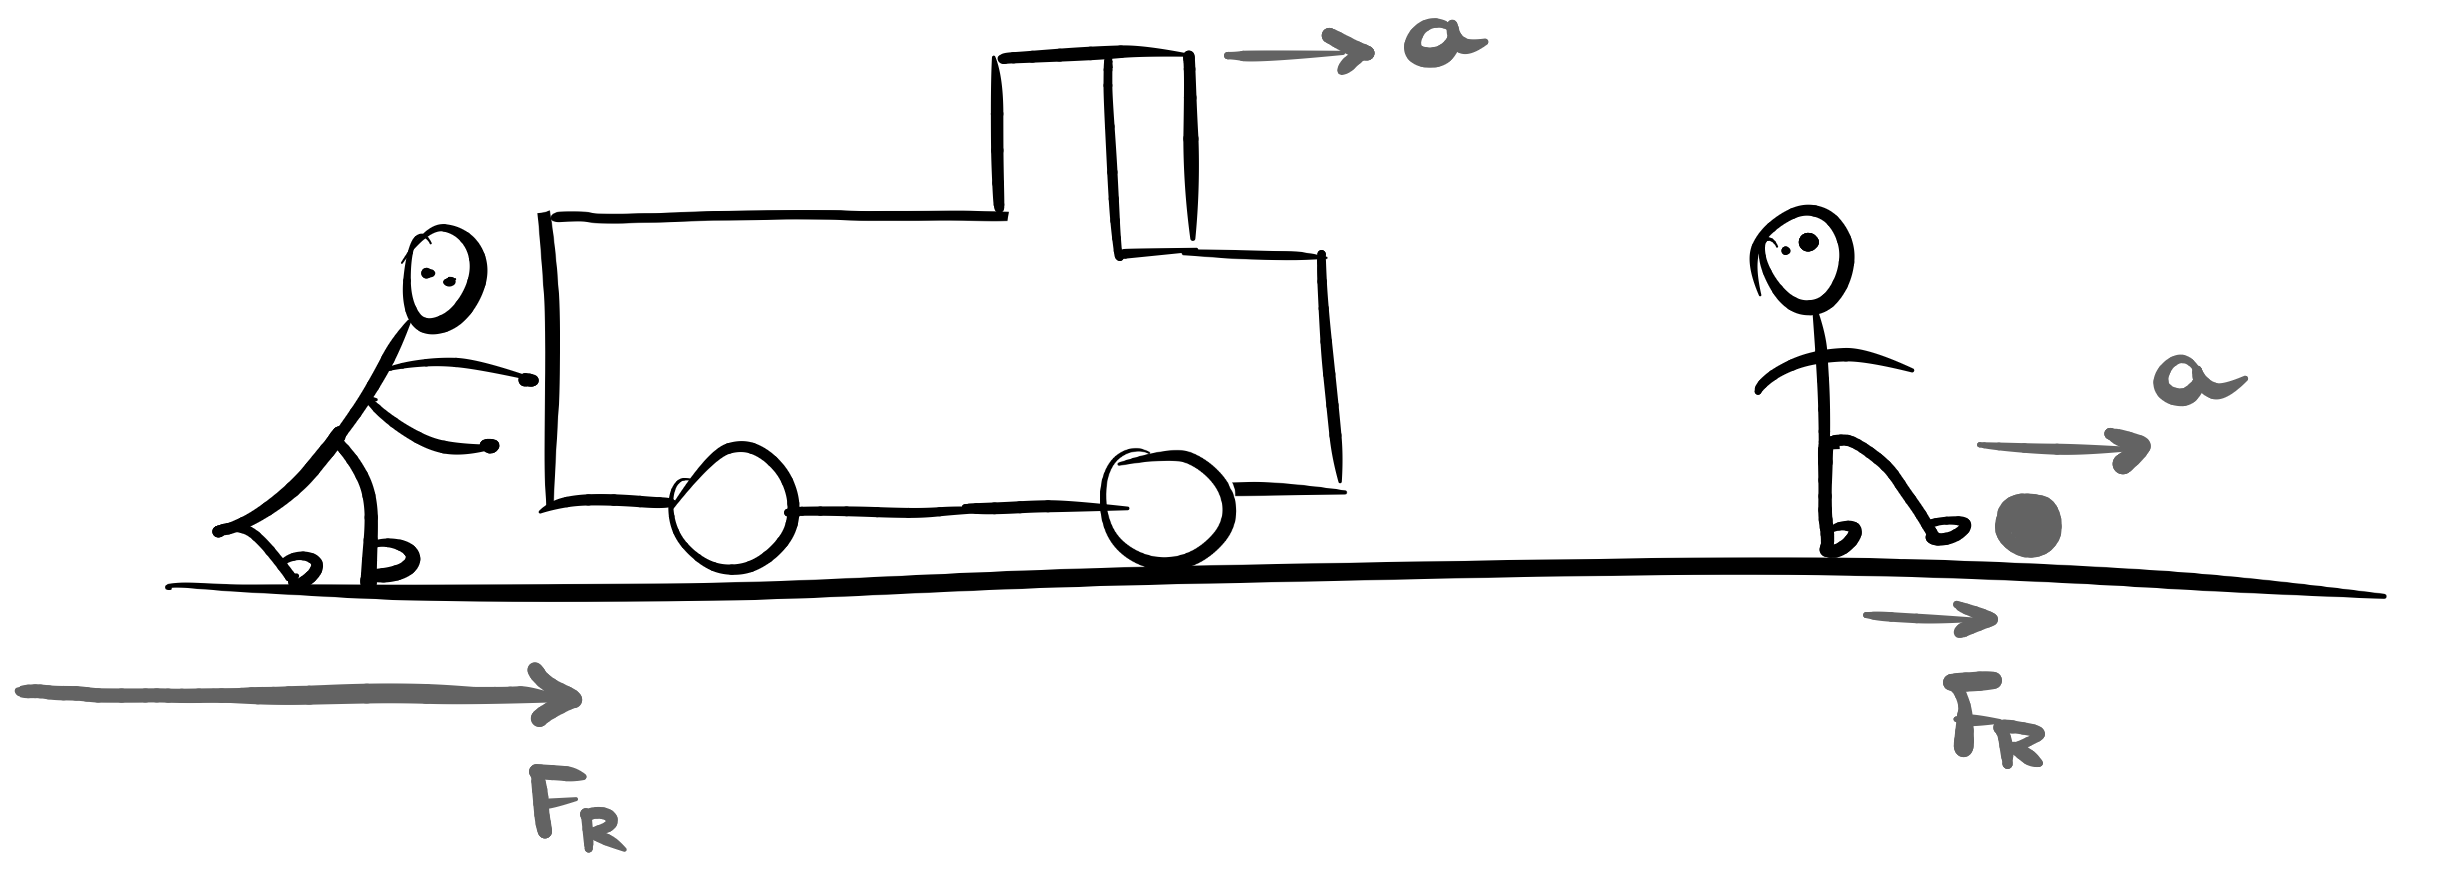
\includegraphics[width=0.6\linewidth]{imagensdinamicanewton/f=ma inercia massa.png}};
  \end{scope}
\end{tikzpicture}
\captionof{figure}{É preciso pouca força para alterar o estado de movimento de um corpo de pouca massa, mas muita força para alterar o estado de movimento de um corpo de muita massa.}
\label{fig_dinamicanewton_f=ma inercia massa}
} 

\vspace{0.3cm}

Com isso, conclui-se que a força resultante -- o agente que altera o estado de movimento de um corpo -- deve ser diretamente proporcional à massa do corpo cujo estado de movimento deseja-se alterar, uma vez que esta mede a capacidade de tal corpo permanecer em seu atual estado de movimento (inércia). É por isso que a massa $m$ é a constante de proporcionalidade que aparece na Segunda lei de Newton: corpos de maior massa (inércia) exigirão uma força maior (agente que causa a variação do movimento) para que se gere a mesma aceleração (variação do movimento). Podemos, inclusive, ler a Segunda Lei de Newton dessa forma:


$$  \underbrace{\text{(agente que causa a variação do movimento)}}_{\text{$F_R$}} = \underbrace{\text{(inércia)} }_{m} \cdot \underbrace{\text{(variação do movimento)}}_{a} .  $$




Logo, no caso do caminhão, como sua massa (inércia) é alta, é preciso mais força para gerar a mesma variação de movimento (aceleração):

$$  \underbrace{ \uparrow \text{(agente que causa a variação do movimento)}}_{\text{$F_R$}} = \underbrace{ \uparrow \text{(inércia)} }_{m} \cdot \underbrace{\text{(variação do movimento)}}_{a} .  $$



\secgfe{Onde é usada}



Essa é, com segurança, a equação mais importante de toda a Física estudada no Ensino Médio. Ela é o alicerce central de toda a mecânica newtoniana, que é a base de toda a Física que se desenvolveu nos 250 anos posteriores a Newton. 

Galileu morre em 1642, mesmo ano em que Newton nasce. Até o desenvolvimento da chamada Física Moderna – que se dá a partir de 1900, com o surgimento da Física Quântica por Planck e, posteriormente, com o desenvolvimento da Teoria da Relatividade Restrita de Einstein, em 1905 – praticamente tudo que é feito em Física neste longo intervalo de tempo é baseado na teoria mecânica de Newton e, consequentemente, na Equação \eqref{eq_dinamica1_segundaleinewton}.

Dito isso, as aplicações possíveis de tal equação dariam, por si só, um livro inteiro. Veremos, nas próximas seções, algumas equações que constituem certas aplicações. Mas que fique claro que o que veremos é apenas um copo d'água -- uma pequena porção do que contém o oceano. As aplicações são as mais diversas, como o estudo de corpos em movimento, o estudo de movimentos oscilatórios, de colisões de corpos, da trajetória e movimento de partículas que se movem sob a ação de um campo elétrico ou magnético, da interação eletrostática entre corpos carregados, etc. De modo geral, para estudar como se dá o movimento -- ou seja, qual é a aceleração -- de um corpo sob a ação de uma força qualquer -- seja ela uma força gravitacional, eletromagnética, elástica ou de qualquer outra natureza -- a Equação \eqref{eq_dinamica1_segundaleinewton} será a base inicial desse estudo: dada a expressão matemática da força, tal equação nos permitirá encontrar a aceleração deste corpo que é gerada pela aplicação de tal força, de tal sorte que, munidos da aceleração, poderemos fazer a descrição cinemática e compreender toda a evolução do movimento.


\secgfe{Erros comuns}

O erro mais comum é não compreender o caráter vetorial da Equação \eqref{eq_dinamica1_segundaleinewton}: trata-se de uma equação que envolve vetores, a força resultante $\vec{F}_R$ e a aceleração $\vec{a},$ respectivamente. Sendo assim, trabalhando com a decomposição vetorial, o mais comum é que façamos uma análise das forças em duas direções perpendiculares e, portanto, independentes.

\vspace{0.3cm}
{
\centering
\begin{tikzpicture}
  \begin{scope}[blend mode=multiply]
    \node {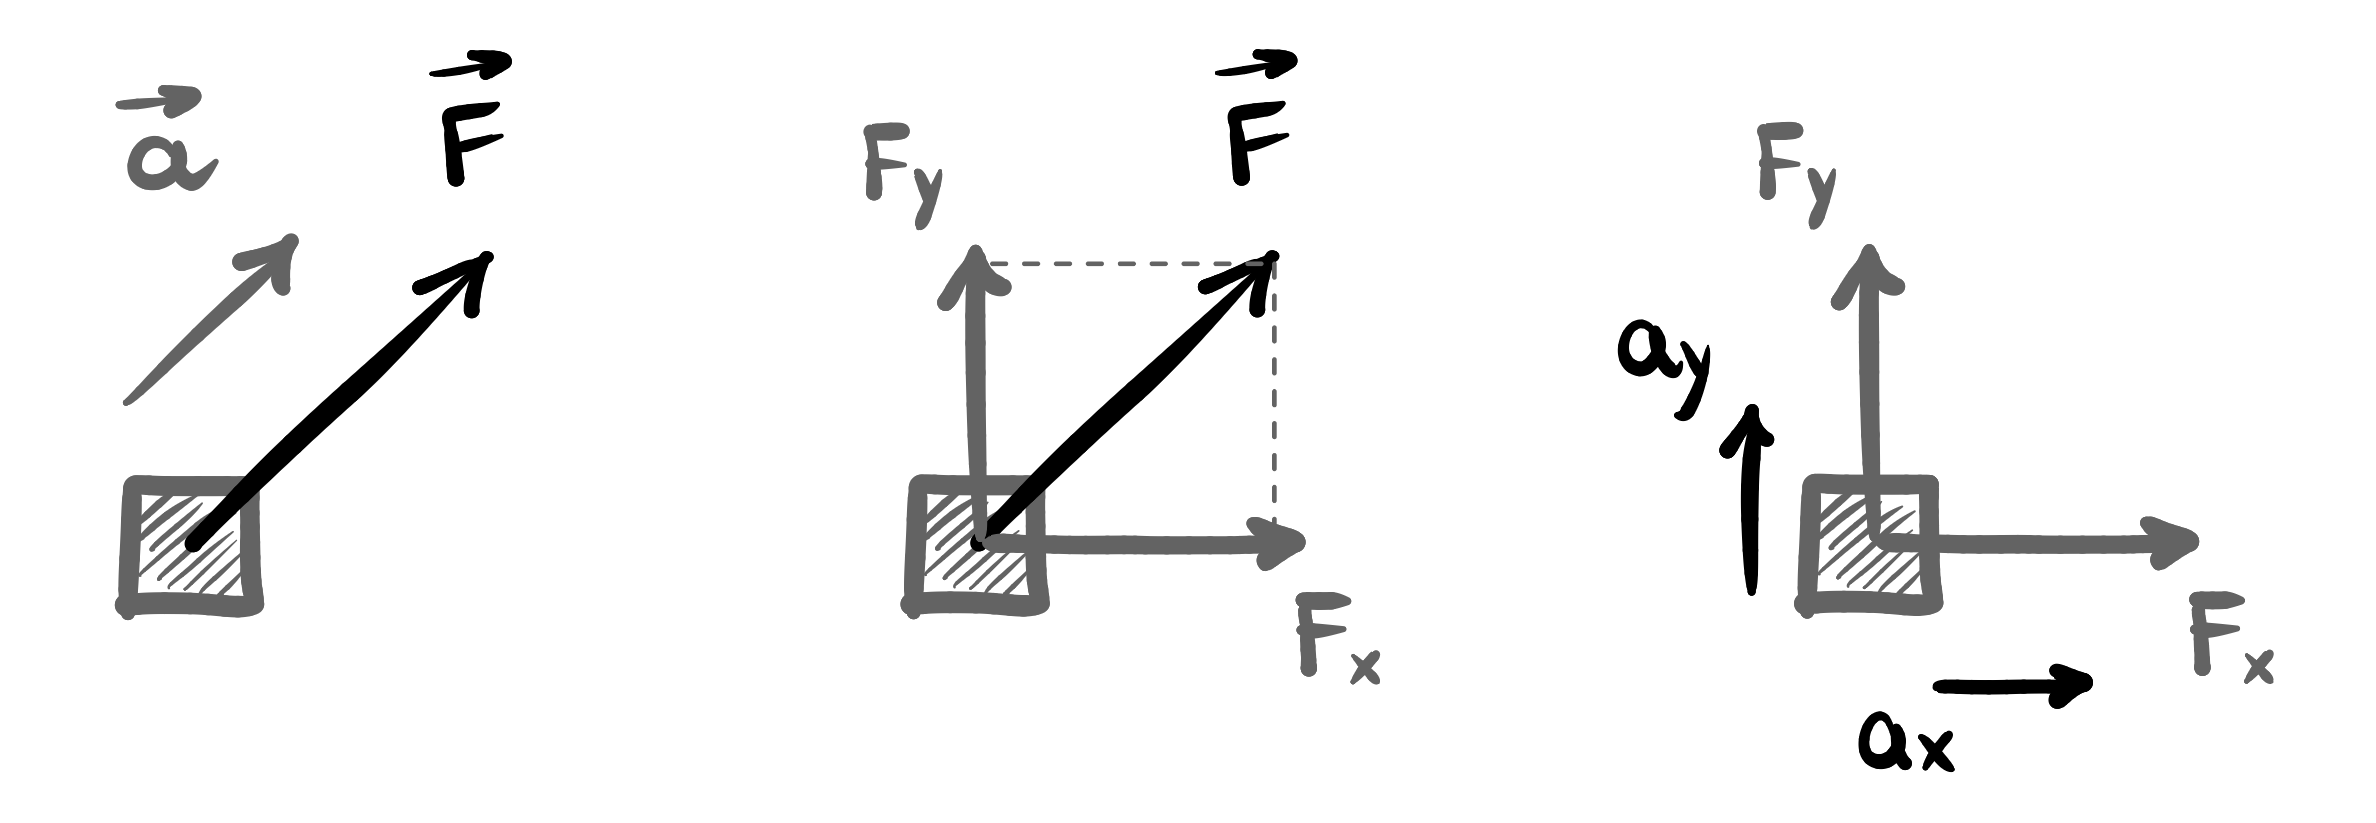
\includegraphics[width=0.6\linewidth]{imagensdinamicanewton/segundaleinewtondecomposicao2.png}};
  \end{scope}
\end{tikzpicture}
\captionof{figure}{A segunda lei de Newton aplicada em duas direções perpendiculares -- e, portanto, independentes.}
\label{fig_dinamicanewton_segundaleinewtondecomposicao2}
} 
\vspace{0.3cm}

Ou seja, como mostra a Figura \ref{fig_dinamicanewton_segundaleinewtondecomposicao2}, podemos compreender a força $\vec{F}$ como sendo a responsável por gerar a aceleração total $\vec a$ da partícula; ou, então, podemos decompor tal força em duas componentes nos eixos perpendiculares $x$ e $y$, originando as forças $\vec{F}_x$ e $\vec{F}_y$. Assim, tais forças gerariam as acelerações $\vec{a}_x$ e $\vec a_y,$ respectivamente. Este segundo caminho será o mais comum: analisarmos a resultante das forças em direções perpendiculares $x$ e $y,$ para compreender a aceleração gerada nessas duas direções.

Dito isso, sendo tal procedimento extremamente comum e corriqueiro na resolução de problemas sobre leis de Newton, os erros mais comuns cometidos pelos estudantes são dois:

\begin{enumerate}
    \item [(i)] Cometer erros na decomposição vetorial.

    Aqui podemos ter os mais variados tipos de erros: não compreender corretamente como funciona a decomposição vetorial, ou então, por lacunas no conhecimento matemático, não saber usar corretamente as razões trigonométricas seno e cosseno para calcular as componentes decompostas. Essa natureza de erros refere-se, majoritariamente, a falhas oriundas da matemática: o aluno não tem uma boa base em geometria/trigonometria e se confunde na decomposição dos vetores e nos cálculos geométricos necessários para fazê-lo.

    Como Galileu percebeu, \textit{``...o grande livro da Natureza está escrito em linguagem matemática, e seus caracteres são triângulos, círculos e outras figuras geométricas, sem os quais é humanamente impossível entender uma única palavra. Sem eles é uma errância, é um desatino vão num labirinto obscuro.''} 

    Sem matemática é impossível estudar Física -- certamente isso já está claro para o leitor ao longo da leitura de um guia de fórmulas matemáticas para o estudo de Física. Mas cabe ressaltar que, daqui em diante, os conhecimentos de matemática -- em particular os de geometria e trigonometria -- se farão mais presentes e relevantes do que nunca. A sua ausência ou insuficiência acaba se tornando o motivo de muitos erros e dificuldades dos estudantes nesse assunto.

    \item [(ii)] Fazer a escolha errada de eixos para a decomposição.


     Sendo necessário na quase totalidade dos problemas de dinâmica fazer a decomposição das forças nos dois eixos perpendiculares, fica a pergunta: \textit{quais eixos devem ser usados?}

 Já sabemos e acordamos que a decomposição de vetores será sempre feita em um par de eixos perpendiculares. Isso ocorre para que possamos usar o Teorema de Pitágoras, as razões trigonométricas no triângulo retângulo e o princípio de que movimentos em direções perpendiculares são independentes; logo, podemos aplicar de forma independente a Equação \eqref{eq_dinamica1_segundaleinewton} nas duas direções distintas $x$ e $y$:


\[
 \vec{F}_R = m\vec a
\quad \xrightarrow{\text{projeção nos eixos}}
\quad
\begin{cases}
F_x = m a_x \\
F_y = m a_y
\end{cases}
\]

Contudo, qual é a melhor escolha de eixos? Mesmo nos restringindo a eixos perpendiculares, existem uma infinidade deles. A Figura \ref{fig_dinamicanewton_segundaleinewtondecomposicao1}, que ilustra o movimento de um pêndulo, destaca três possíveis escolhas de pares de eixos $xy$ que podem ser utilizados para a decomposição das forças e análise da dinâmica do movimento.


\vspace{0.3cm}
{
\centering
\begin{tikzpicture}
  \begin{scope}[blend mode=multiply]
    \node {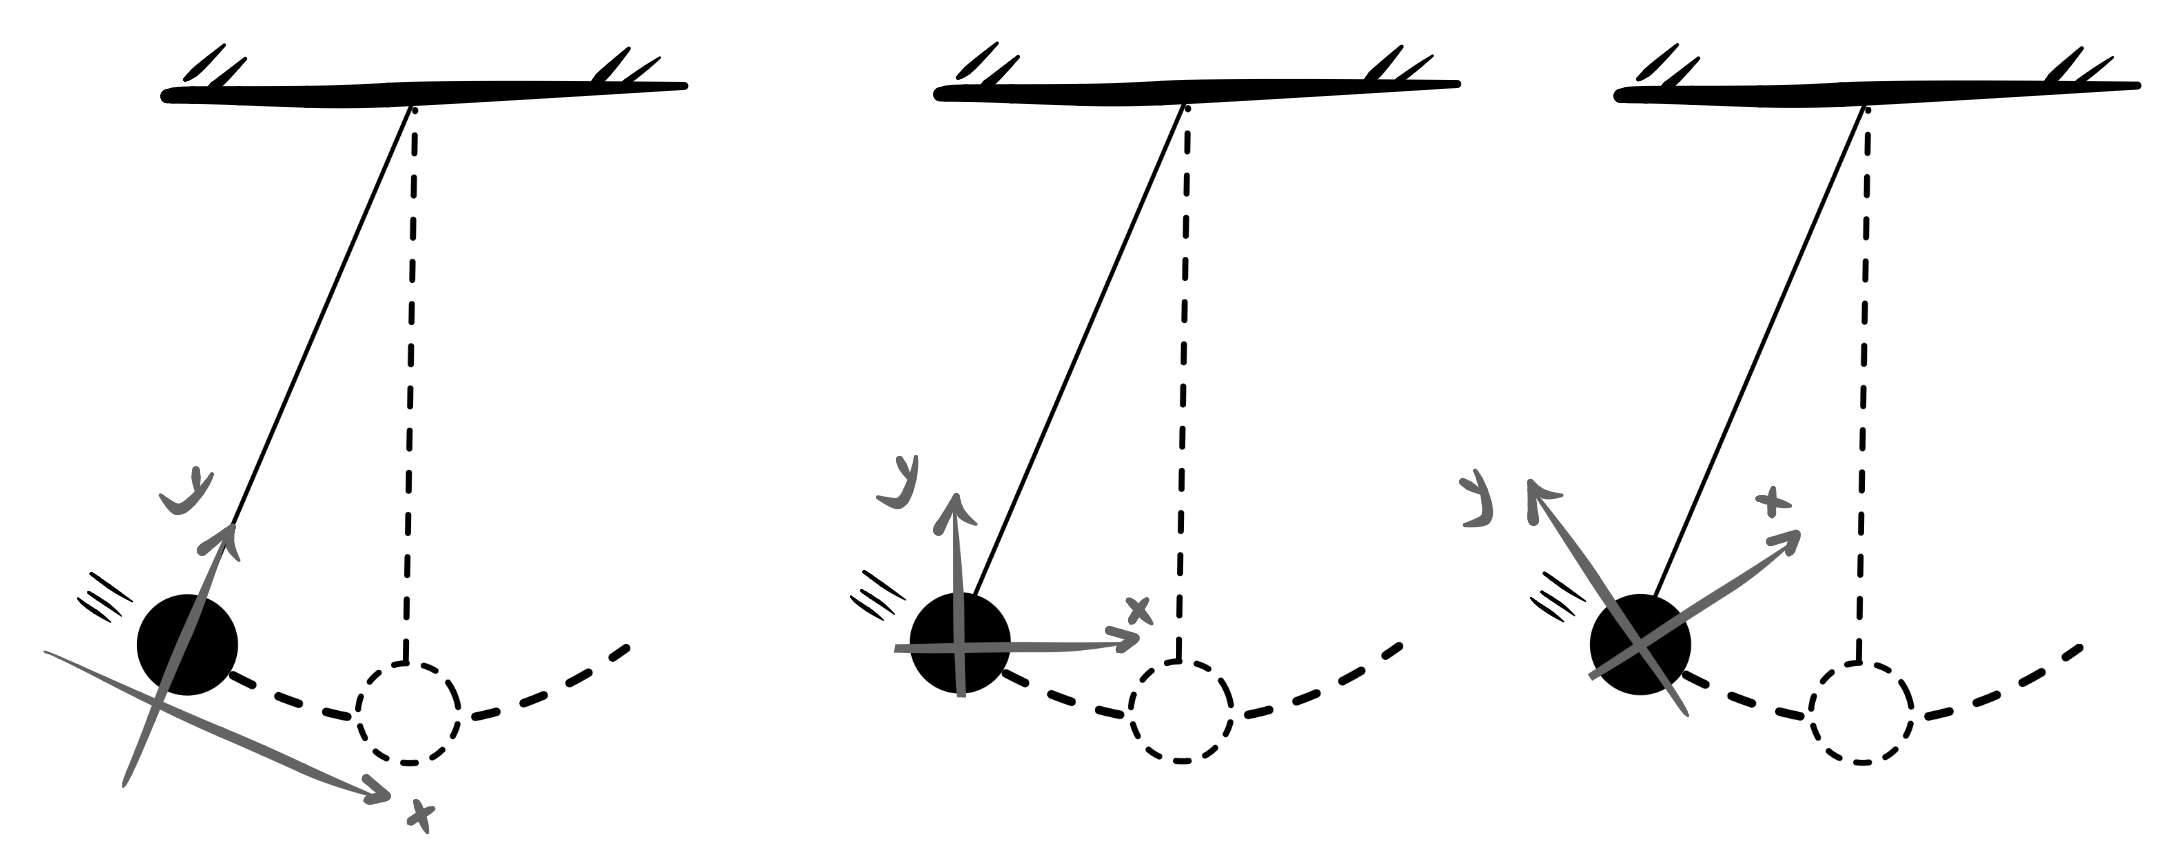
\includegraphics[width=0.6\linewidth]{imagensdinamicanewton/segundaleinewtondecomposicao1.png}};
  \end{scope}
\end{tikzpicture}
\captionof{figure}{Possíveis escolhas de eixos para fazer a decomposição vetorial das forças.}
\label{fig_dinamicanewton_segundaleinewtondecomposicao1}
} 
\vspace{0.3cm}


     Se o estudante não souber fazer essa escolha corretamente, a análise e o desenvolvimento matemático do problema se tornará (sem exageros) 5 vezes mais difícil, e acabará levando o leitor, com quase total certeza, a conclusões equivocadas e erros no meio do caminho. Esse é, possivelmente, o principal erro cometido em problemas que envolvam a Equação \eqref{eq_dinamica1_segundaleinewton}. 
     
     Para saciar a curiosidade dos mais ansiosos, a escolha mais adequada dos eixos de decomposição da situação da Figura \ref{fig_dinamicanewton_segundaleinewtondecomposicao1} é a da primeira imagem. Em breve entenderemos o porquê, e também faremos alguns exemplos para nos familiarizarmos com esse procedimento e conseguirmos sempre acertar nessa escolha de eixos, mas já adianto ao leitor qual será a regra de ouro para fazer a escolha correta:

 
        \textbf{A escolha dos eixos para fazer a decomposição vetorial e análise das forças que atuam em um corpo para que se aplique a Equação \eqref{eq_dinamica1_segundaleinewton} é tal que um dos eixos seja sempre paralelo ao vetor velocidade da partícula naquele ponto.}\footnote{A resultante das forças nesse eixo será responsável por gerar a aceleração tangencial (ou escalar) da partícula: aquela aceleração responsável por variar o módulo da sua velocidade.} 

         O segundo eixo já fica automaticamente definido pela exigência de ter de ser perpendicular ao primeiro.
   
    
\end{enumerate}




\secgfe{Observações}


A própria Equação \eqref{eq_dinamica1_segundaleinewton} já evidencia que a força é uma grandeza vetorial: ela precisa de módulo, direção e sentido para ser determinada. O vetor força sempre apontará na mesma direção e sentido do vetor aceleração, uma vez que o primeiro é o responsável por gerar o último. Logo, em um movimento retilíneo acelerado (aceleração e velocidade no mesmo sentido) a força terá o mesmo sentido da velocidade, enquanto que em um movimento retilíneo retardado (aceleração e velocidade em sentidos contrários) o vetor força terá sentido oposto ao do vetor velocidade.

A unidade de massa no Sistema Internacional de unidades de medida (SI) é o kg, enquanto que a unidade de aceleração no SI é m$\cdot$s$^{-2}.$ Assim, a unidade de força no SI é $\text{kg}\cdot\text{m}\cdot\text{s}^{-2}$, a que damos o nome de Newton (N):

$$ \boxed{\text{kg}\cdot\text{m}\cdot\text{s}^{-2} = N.}$$

Logo, se faz-se uma força em um objeto de $2$ kg de massa e gera-se nele uma aceleração de $5$ m/s$^2,$ tal força deve ser igual a
$$ F_R = ma \implies F_R = 2 \text{ kg} \cdot 5 \text{ m/s}^2 \implies F_R = 10 \text{ N.}$$

Como estamos introduzindo agora a Dinâmica, cabe fazer uma observação importante sobre a diferença entre ela e a Cinemática, que constituiu todo nosso estudo até então.  A Cinemática e a Dinâmica tratam do movimento, mas não fazem o mesmo tipo de pergunta. A Cinemática descreve, enquanto a Dinâmica explica.

Quando escrevemos
\[
s(t)=s_0+v_0 t+\frac12 at^2,
\]
estamos apenas descrevendo como a posição varia no tempo. A equação nada nos diz sobre \emph{por que} a aceleração tem determinado valor. Ela aceita a aceleração como um dado e constrói, a partir dela, o movimento.

A Segunda Lei de Newton muda completamente o cenário:

$$ \vec F_R = m\vec a.$$
 

Agora, a aceleração deixa de ser um dado arbitrário e passa a ser consequência de algo físico: a força resultante. Essa é a transição essencial: na Cinemática, a aceleração é um dado que aceitamos; já na Dinâmica, a aceleração é determinada por causas.


Em termos conceituais, a Segunda Lei introduz uma estrutura de causalidade, a de que a aceleração é causada pela força:
\[
\text{força resultante} \longrightarrow \text{aceleração}.
\]

A força não produz velocidade diretamente. Ela produz variação da velocidade.  Esse detalhe, aparentemente pequeno, é o que diferencia a mecânica newtoniana da aristotélica e é a base de toda a mecânica clássica, como vimos. 

É por isso que um corpo pode mover-se com velocidade constante mesmo sob ausência total de forças --- algo que a intuição pré-newtoniana não aceitava. O movimento uniforme não precisa de causa contínua; apenas a mudança do movimento exige isso.

% Essa estrutura causal é determinista: dadas as condições iniciais do movimento (onde a partícula estava inicialmente e qual era sua velocidade no instante inicial do movimento) e conhecidas as forças atuantes, o movimento está completamente determinado. Essa foi uma das grandes revoluções intelectuais da ciência moderna.


Desse modo, a Cinemática responde à pergunta ``como o corpo se move?'', enquanto a Dinâmica responde à pergunta ``por que ele se move assim?'' A primeira descreve trajetórias; a segunda constrói o mecanismo que as produz. 

\medskip

Uma outra observação bastante importante é o fato de que a Segunda Lei de Newton afirma que a força resultante determina a aceleração, mas ela não nos diz o que é a força. Ela não explica por que a Terra atrai a Lua; ou por que cargas elétricas interagem; ou por que dois corpos em contato exercem forças normais, etc. Ela apenas estabelece o que acontece quando uma força está presente.

Essa distinção é fundamental. Muitas vezes o estudante imagina que $ \vec F = m\vec a$ seja uma teoria completa do movimento. Não é. Ela é uma estrutura geral dentro da qual diferentes interações podem ser inseridas. 

A gravidade, a força elétrica e a força elástica, por exemplo, são descritas respectivamente por


$$ F_G = \,G\frac{Mm}{r^2}, \quad F_E = K\frac{q_1 q_2}{r^2} \quad \text{e} \quad  F = -k x  $$

\vspace{0.3cm}
{
\centering
\begin{tikzpicture}
  \begin{scope}[blend mode=multiply]
    \node {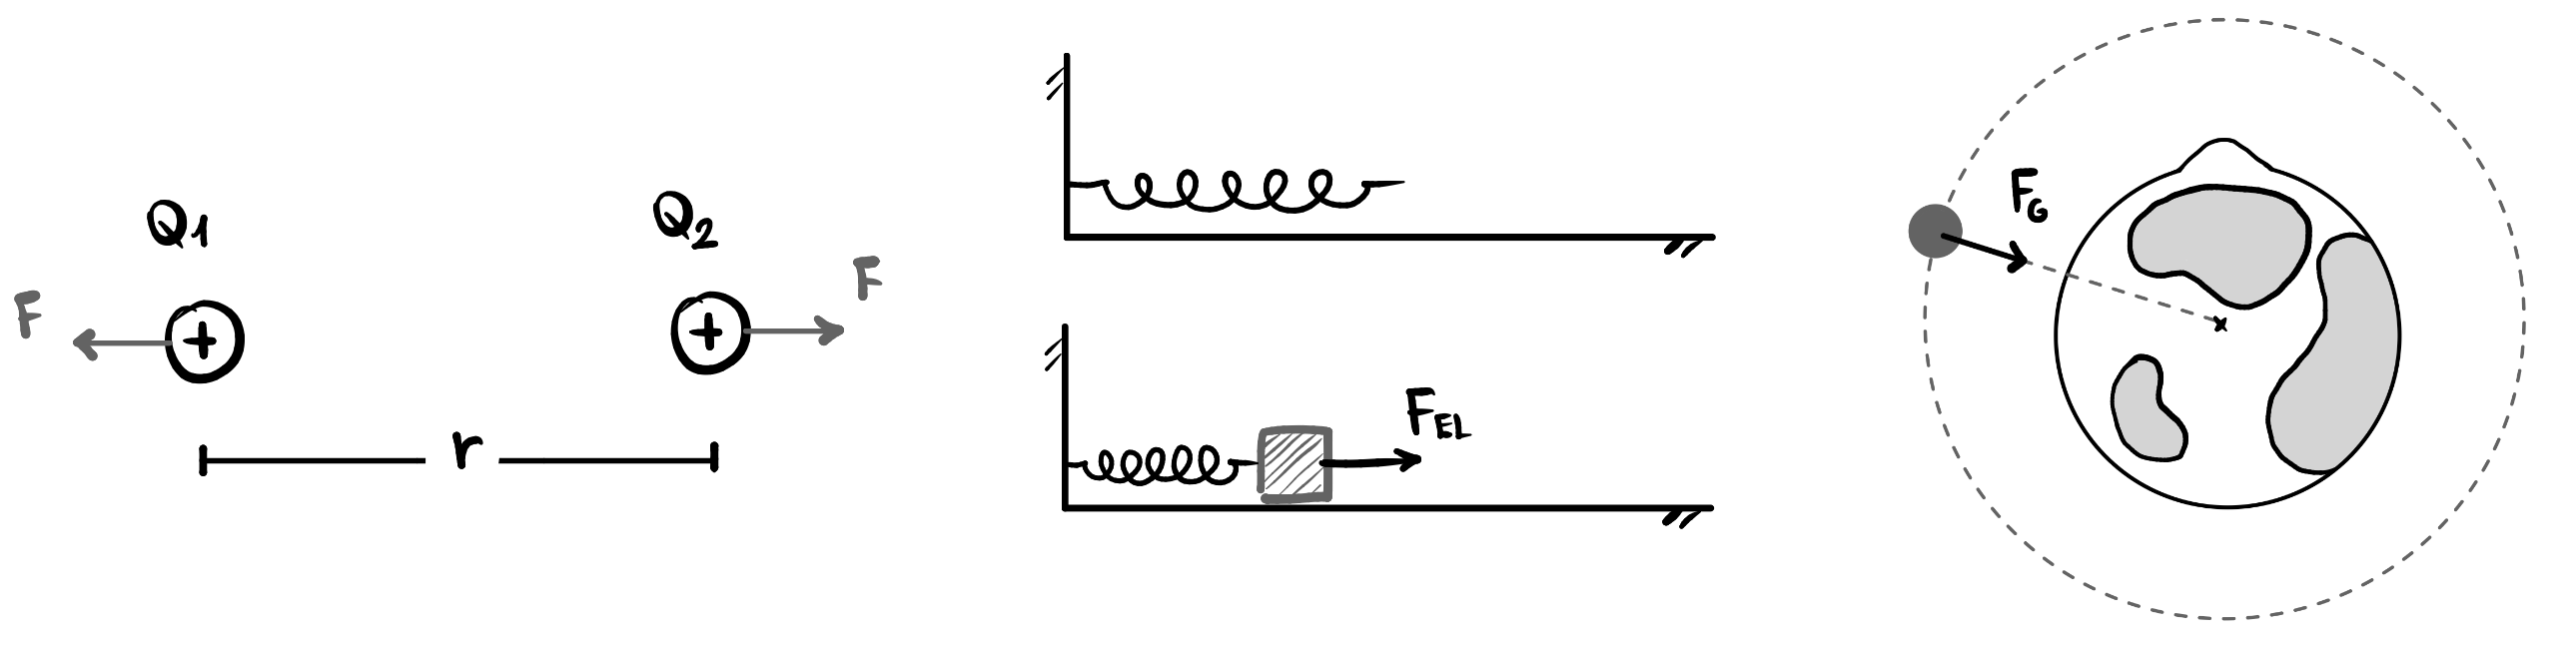
\includegraphics[width=1.0\linewidth]{imagensdinamicanewton/dinamicaforcasrepresentacaoexemplo.png}};
  \end{scope}
\end{tikzpicture}
\captionof{figure}{Representação das forças de interação elétrica, elástica e gravitacional.}
\label{fig_dinamicanewton_dinamicaforcasrepresentacaoexemplo}
} 
\vspace{0.3cm}

Essas três forças se encontram representadas, respectivamente, na Figura \ref{fig_dinamicanewton_dinamicaforcasrepresentacaoexemplo}: a força elétrica é a força de interação entre corpos carregados eletricamente (e é estudada em detalhes no volume III dessa coleção), a força elástica é a força que se manifesta em uma mola comprimida, e é estudada na Equação \eqref{eq_dinamicanewton_leihooke}; e, por fim, a força gravitacional é a força de interação entre corpos massivos -- a força de interação entre a Terra e a Lua, por exemplo -- e será estudada na Equação \eqref{eq_gravitacao_leigravitacaouniversal}.

Essas expressões não vêm da Segunda Lei. Elas são leis adicionais, obtidas por experimentos, e descrevem tipos específicos de interação. A Segunda Lei, portanto, atua como uma espécie de tradutor: como já vimos na Cinemática, a aceleração é a linguagem do movimento. Já as forças são a linguagem da interação -- sempre que corpos interagirem, tal interação será por meio de uma força (magnética, elétrica, elástica, gravitacional, etc). Assim, a segunda lei faz a tradução de como as forças -- a linguagem da interação entre corpos -- produzem aceleração, isto é, a linguagem do movimento. Desse modo, a Segunda Lei permite obter, por meio de como corpos interagem (forças), o elemento central (a aceleração) que a Cinemática precisa para fazer a descrição do movimento como um todo. O procedimento, portanto, sempre é:

\begin{enumerate}
\item  Escolhe-se o corpo cujo movimento desejamos estudar.
\item  Identificam-se as forças que nele atuam.
\item  Somam-se as forças vetorialmente.
\item  Com a Segunda Lei, determina-se a aceleração do corpo.
\item  Com a aceleração, a Cinemática já tem tudo o que precisa para descrever o movimento do corpo.
\end{enumerate}


O segundo exemplo que faremos na sequência ilustrará com clareza a execução desse procedimento.


É importante perceber que a natureza das forças pertence a outras teorias. Essa separação mostra a grandeza e vastidão da aplicabilidade da Equação \eqref{eq_dinamica1_segundaleinewton}: ela permite que a mecânica clássica seja um arcabouço geral, dentro do qual diferentes fenômenos podem ser descritos, desde que se conheça a estrutura das forças de cada fenômeno específico. E é por isso que tal equação é tão central no estudo da Física.



\vspace{0.3cm}

\begin{exemplo}[Nível I]\label{exemplo_dinamica1_eq_dinamica1_segundaleinewtonex01}

Uma partícula de massa $m=2$kg tem um movimento retilíneo e acelerado, sob a ação de apenas duas forças, como mostra a Figura \ref{fig_dinamicanewton_f=ma1} (p.~\pageref{fig_dinamicanewton_f=ma1}). Se o módulo da sua aceleração é $a=3$ m/s$^2$ e $F_1 = 50N,$ calcule o valor de $F_2.$



\resolucao

Pela segunda lei de Newton temos

$$ F_R = ma = 2 \text{ kg} \cdot 3 \text{m/s}^2 \implies \boxed{ F_R = 6 \text{N}.}$$

A $\vec F_R$ é, na verdade, um vetor: é a soma vetorial de todas as forças que atuam no corpo, computando a força resultante que nele atua, ou seja:

$$ \vec F_R = \vec F_1 + \vec F_2.$$

Já estudamos em detalhes a soma de vetores, que no caso da Figura \ref{fig_dinamicanewton_f=ma1}, em que eles apontam em direções contrárias, o módulo do vetor soma é dado pela diferença entre os módulos dos vetores somados, isto é:

$$ F_R = F_1 - F_2 \implies 6 = 50 - F_2 \implies \boxed{F_2 = 44 \text{N.}} $$



\end{exemplo}

\vspace{0.3cm}



\begin{exemplo}[Nível II]\label{exemplo_dinamica1_eq_dinamica1_segundaleinewtonex02}

Um bloco se move em linha reta em um plano horizontal. Sua velocidade inicial é $v_0=20$ m/s e ele enfrenta uma força de atrito constante de valor igual a $10$ N. Sendo a massa do bloco $m=2$ kg, encontre a distância total que ele percorre até ser totalmente desacelerado pelo atrito.

\resolucao

O problema se dividirá em duas etapas: a primeira é a aplicação da Dinâmica, que nos fornecerá o resultado para segunda etapa, a análise Cinemática:

\begin{enumerate}
    \item [(i)] Dinâmica.

    Usando a Segunda Lei de Newton -- sendo a força de atrito $F_{AT}$ a única força que atua na direção do movimento -- teremos, para essa direção:

    $$ F_{AT}  = F_R = ma \implies 10 = 2 a \implies \boxed{a = 5 \text{ m/s}^2.}  $$

    Logo, como a equação é vetorial, isto é:

    $$ \vec F_{R} = m \vec a,$$

    \noindent a aceleração apontará exatamente na mesma direção e sentido da força de atrito (que é a força resultante nessa situação), isto é, no sentido oposto ao do movimento (velocidade). Teremos, portanto, um movimento retardado, como era esperado. Sendo o valor de tal aceleração constante, concluímos que se trata de um MUV, e podemos usar nossos conhecimentos de Cinemática sobre tal movimento para dar sequência no raciocínio.

    \item [(ii)] Cinemática.

    Daqui em diante tudo se reduz a um problema já resolvido por nós algumas vezes. Temos um bloco com velocidade inicial $v_0=$ 20 m/s, sofrendo uma desaceleração constante de $5$ m/s$^2$, e queremos saber a distância que ele percorre até parar, isto é, até atingir $v=0.$ Por se tratar de um MUV, uma boa equação para computar isso sem necessidade de cálculos intermediários é a Equação de Torricelli:

    $$ \cancelto{0}{v^2} = v_0^2 -2a \Delta s \implies \Delta s = \dfrac{v_0^2}{2a} = \dfrac{20^2}{2 \cdot 5} \implies \boxed{\Delta s = 40 \text{ m} .}$$
\end{enumerate}

Perceba como estamos empilhando conhecimentos. O passo $(ii)$ foi um problema já resolvido por nós na Cinemática. Com a Dinâmica o que fizemos foi construir um arcabouço teórico que nos permite, dadas as influências físicas que um corpo sente (forças), encontrar a sua aceleração. Munidos da aceleração -- caso ela seja constante -- todo o problema se reduzirá aos problemas já estudados de MUV.\\

Desse modo, quase todo problema de Dinâmica vai envolver Cinemática: as leis de Newton serão o passo inicial para encontrar a aceleração e, com essa, o restante do problema seguirá pelos caminhos já conhecidos da Cinemática.


\end{exemplo}

% \vspace{0.3 cm}

% Essa é uma amostra grátis do livro de Guia de Fórmulas Explicadas, de autoria do professor Felipe Guisoli. A previsão é que ele seja lançado em agosto de 2026. Até lá, você pode estudar toda a Física do ensino médio com essa mesma abordagem -- didática, profunda e completa -- pelo curso completo de Física do Universo Narrado, o Lições de Física, ministrado pelo mesmo professor.

% O QR Code abaixo te direcionará para um grupo exclusivo em que você terá acesso a uma oferta especial no dia 02/março para se matricular no UN.

% {
% \centering
% 
\includegraphics[width=0.4\linewidth]{imagensintro/qr-code (6).png}
% \captionof{figure}{Entre no grupo VIP para receber em primeira mão a oferta especial para se tornar aluno do UN em 2026.}
% \label{figura_lancamentoforadacurva2026}
% } 

%\newpage

\vspace{0.3cm}


%  \begin{exemplo}[Nível III]\label{exemplo_dinamica1_eq_dinamica1_segundaleinewtonex03}

% Dois blocos, de massas $m_1 = \SI{3{,}0}{kg}$ e $m_2 = \SI{2{,}0}{kg}$,
% estão em contato e são empurrados juntos por uma força horizontal
% $F = \SI{20}{N}$ aplicada sobre $m_1$, numa superfície sem atrito.
% Determine:

% \begin{enumerate}
%   \item [a)] a aceleração do conjunto;
%   \item [b)] a intensidade da força de contato $F_c$ que $m_1$ exerce sobre
%   $m_2$.
% \end{enumerate}

%  \resolucao

% O conceito mais importante deste problema está em perceber que
% $\vec{F}_R = m\vec{a}$ pode ser aplicada a \emph{subsistemas} ---
% não apenas ao objeto isolado ou ao sistema completo. A escolha inteligente
% do sistema de análise é, aqui, o cerne da solução.

% \medskip 

% \noindent\textit{a)} Sistema completo ($m_1 + m_2$):

% Quando tratamos os dois blocos como um único sistema, a força de contato
% entre eles torna-se uma força \emph{interna} --- e forças internas não
% aparecem na resultante externa do sistema. A única força externa
% horizontal é $F$. Portanto:

% \[
%   F = (m_1 + m_2)\,a
%   \;\Longrightarrow\;
%   a = \frac{F}{m_1 + m_2} = \frac{20}{3{,}0 + 2{,}0} = \frac{20}{5{,}0}
%     = \SI{4{,}0}{m/s^2}.
% \]

% \noindent\textit{b)} Subsistema $m_2$ isolado:

% O bloco $m_2$ não sente a força $F$ diretamente --- ele só ``sabe'' que ela
% existe porque $m_1$ o empurra. A única força horizontal sobre
% $m_2$ é exatamente a força de contato $F_c$. Aplicando $F_R = m_2\,a$:

% \[
%   F_c = m_2\,a = 2{,}0 \cdot 4{,}0 = \SI{8{,}0}{N}.
% \]

% % \noindent Verificação pelo subsistema $m_1$: sobre $m_1$ atuam $F$
% % para a frente e $F_c$ para trás (reação de $m_2$ sobre $m_1$, pela
% % Terceira Lei --- que formalizaremos na seção seguinte):

% % \[
% %   F - F_c = m_1\,a \;\Longrightarrow\; 20 - 8{,}0 = 3{,}0 \cdot 4{,}0
% %   = 12 \;\checkmark
% % \]

% \noindent O resultado $F_c = \SI{8{,}0}{N}$ merece uma leitura
% qualitativa: a força de contato não é $F$, nem $F/2$. Ela é a fração
% da força total que ``coube'' a $m_2$ na distribuição proporcional às
% massas:

% \[
%   F_c = F \cdot \frac{m_2}{m_1 + m_2} = 20 \cdot \frac{2{,}0}{5{,}0}
%       = \SI{8{,}0}{N}.
% \]

% \noindent Essa proporcionalidade é uma das primeiras manifestações de
% algo que o leitor encontrará repetidamente: em sistemas acoplados sem
% atrito, cada parte recebe da força total exatamente a parcela
% proporcional à sua inércia.

%  \end{exemplo}


\begin{exemplo}[Nível III]\label{exemplo_dinamica1_eq_dinamica1_segundaleinewtonex03}

Um corpo de massa $m$ parte do repouso. Uma força resultante constante $F$ atua sobre
ele por um intervalo de tempo $T$, após o que é imediatamente invertida --- mantendo
módulo $F$, porém no sentido contrário --- e continua atuando indefinidamente. Determine
o tempo que o corpo leva para retornar à posição de partida após a inversão, e a
velocidade com que passa por ela.



\resolucao

Sendo as forças constantes, as acelerações geradas por elas -- dadas por $a = F/m$ -- também serão constantes, de modo que os movimentos serão uniformemente variados. Na primeira fase, o corpo acelera a partir do repouso por um tempo $T$, atingindo

$$ v_{\max} = \cancelto{0}{v_0} + aT = \frac{FT}{m}, \qquad d_1 = \cancelto{0}{v_0} \cdot t  + \frac{1}{2}aT^2 = \frac{FT^2}{2m}. $$

Esta é a maior velocidade do movimento. Tomando $t = 0$ no instante da inversão e a
origem na posição de partida, a posição na segunda fase é

$$ x(t) = d_1 + v_{\max}\,t - \frac{1}{2}a\,t^2. $$

O retorno à origem ocorre quando $x(t) = 0$. Substituindo e multiplicando por $2m/F$:

$$ t^2 - 2Tt - T^2 = 0, $$

\noindent cujas raízes são

$$ t = T\!\left(1 \pm \sqrt{2}\right). $$

Tomando a raiz positiva:

$$ \boxed{t_{\text{retorno}} = T\!\left(1 + \sqrt{2}\right).} $$

A velocidade ao retornar à origem é

$$v = v_\text{max} - at \implies  v = \frac{FT}{m} - \frac{F}{m}\cdot T\!\left(1+\sqrt{2}\right)
     = -\frac{FT\sqrt{2}}{m}, $$

\noindent cujo módulo é

$$ \boxed{|v| = \frac{FT\sqrt{2}}{m} = \sqrt{2}\cdot v_{\max}.} $$

O corpo retorna à posição de partida com velocidade $\sqrt{2} \approx 1{,}41$ vezes
maior do que a velocidade máxima atingida durante a ida. Curioso, não?




\end{exemplo}

\vspace{0.3cm}









\begin{secnivel}[Peso]{I}{Peso}
  
  \eqLdois{exp}{eq_dinamicanewton_peso=mg}{P = mg}

\end{secnivel}






\secgfe{De onde vem}

Estudaremos em mais detalhes a força de interação entre corpos massivos, chamada de força gravitacional,\footnote{Ao estudar em mais detalhes a Lei da Gravitação Universal vamos entender como a Equação \eqref{eq_dinamicanewton_peso=mg} da força peso é uma lei experimental particular da lei da Gravitação de Newton.} cuja lei é dada pela Equação \eqref{eq_gravitacao_leigravitacaouniversal}. 

A força peso é justamente a força de interação gravitacional que todos os corpos aqui na Terra sentem, devido à atração gravitacional realizada pela Terra. Ela é dirigida para o centro da Terra, o que, para fins práticos, significa ser dirigida para o chão: é a força que faz com que os corpos caiam.

Experimentos feitos por Galileu evidenciaram que corpos de diferentes pesos em queda livre -- isto é, sob a ação exclusiva da força peso -- caem juntos. Ou seja, mesmo tendo massas diferentes, os corpos caem com a mesma aceleração $g$, que, na superfície da terra, é de $g \approx 9.81 $m/s$^2$. Ou seja, sendo $P$ o valor da força peso, e usando a Equação \eqref{eq_dinamica1_segundaleinewton}, teríamos que, sob a ação exclusiva da força peso, isto é, $F_R =P,$ teríamos:

$$ F_R = P = ma,$$


\noindent e, sendo $g$ a aceleração com os corpos caem sob ação da força peso -- e ela é a mesma independente da massa, como observado pelos experimentos -- temos

$$ P = mg,$$

\noindent que é a equação que queríamos construir.


\secgfe{Onde é usada}

Em praticamente todos os problemas envolvendo as leis de Newton. Sendo a quase totalidade desses problemas no contexto do planeta Terra, uma força que estará sempre presente, naturalmente, será a força peso. 

A aplicação mais direta é a queda livre e o lançamento vertical. Quando
um corpo é abandonado ou arremessado na vertical, o peso é a única força
que atua (desprezando o ar), e a Segunda Lei fornece imediatamente
$a = P/m = g$. É daqui que vem a aceleração gravitacional: ela não é
uma constante que ``existe por si só'' --- ela é a razão entre o peso
e a massa do corpo, e o fato de ser a mesma para todos os corpos é uma
consequência da proporcionalidade $P \propto m$ que a própria fórmula
expressa. Galileu não sabia escrever $P = mg$; mas foi exatamente isso
que ele descobriu ao soltar objetos de alturas diferentes em Pisa.

No estudo do plano inclinado, que veremos na Equação \eqref{eq_dinamicanewtoniana_gsintheta}, o peso é
decomposto em duas componentes: uma paralela ao plano, responsável pela
aceleração do objeto ao longo da rampa, e outra perpendicular, que
equilibra a força normal exercida pelo plano. Toda essa análise vetorial começa com o vetor
$\vec{P} = m\vec{g}$. O mesmo ocorre nos sistemas de polias, nos quais as tensões no fio são
determinadas a partir do peso dos blocos envolvidos: a polia redistribui
forças, mas não cria nem destrói peso. 

A Equação \eqref{eq_dinamicanewton_peso=mg}, portanto, será uma das mais presentes em nosso estudo daqui em diante.


\secgfe{Erros comuns}

O erro mais comum não seria tanto da aplicação em si da Equação \eqref{eq_dinamicanewton_peso=mg}, mas sim de uma interpretação dela: a força peso é maior quanto mais massa o corpo tiver, o que pode levar muitos a intuir que a aceleração com que corpos mais massivos caem seja maior, pelo fato da força que os puxa para baixo ser maior. Contudo, como a massa aparece na equação da força peso e também na equação da Segunda Lei de Newton, este efeito acaba se cancelando, fazendo com que corpos de diferentes massas tenham sempre a mesma aceleração quando sob a ação exclusiva da força peso. Isso pode ser facilmente mostrado usando a força peso como força resultante na Segunda Lei de Newton:

\begin{align}
    F_R &= ma \nonumber \\
    P &= ma  \nonumber \\
    \cancel mg &= \cancel ma, \nonumber 
\end{align}

\noindent de onde conclui-se que 

$$  \boxed{  a = g,} $$

\noindent ou seja, independente da massa, todos os corpos, sob ação única e exclusiva da força peso, caem com a mesma aceleração da gravidade $g.$ É por isso que o movimento de queda livre -- queda sob a ação exclusiva da gravidade -- é um exemplo de MUV, isto é, um movimento com aceleração constante.

\secgfe{Observações}

É importante perceber a diferença entre a massa $m$ de um corpo, que é uma propriedade intrínseca do corpo e mede a quantidade de matéria que ele contêm; do seu peso $P,$ que é uma propriedade que depende da sua massa $m$, mas também do valor do campo gravitacional $g$ da região na qual o corpo está inserido.

Considere, por exemplo, um indivíduo de massa $70$ kg. Na terra, em que a gravidade é $g_T \approx 10$ m/s$^2$, seu peso é

$$ P = mg = 70 \cdot 10 = 700 \text{ N,}$$

\noindent enquanto na lua, onde a gravidade é $g_L \approx 1.6$ m/s$^2$, sua massa -- propriedade intrínseca do indivíduo -- continua sendo de 70 kg, mas seu peso passa a ser de

$$ P = mg = 70 \cdot 1.6 = 112 \text{ N.}$$

Isso não quer dizer que o indivíduo ``\textit{emagreceu}'' ao ir para a lua -- sua massa continua sendo a mesma: 70 kg. Lá, contudo, como a gravidade é menos intensa, a força que o puxa para baixo e o mantém preso no chão -- o seu peso -- é menos intensa. É comum, ao se \textit{pesar} em uma balança, ler o resultado e dizer que o seu peso é de 70 kg. Isso, contudo, estaria impreciso do ponto de vista físico: sua massa é de 70 kg, não o seu peso. A massa informada é um propriedade específica sua, enquanto que o seu peso é uma força que é proporcional à sua massa, mas também depende da região em que você está (por depender do valor da gravidade).


\vspace{0.3cm}

\begin{exemplo}[Nível I]\label{exemplo_dinamicanewton_p=mg01}

Um corpo de massa $m=3$ kg é lançado verticalmente para cima com velocidade de 12 m/s. Se ele enfrenta, ao longo de toda a sua subida, uma força de resistência do ar constante e igual a $6$ N, qual é a altura máxima que ele atinge?

\resolucao

Para problemas desse tipo sempre assumimos que a situação se passa na superfície da Terra, na qual a gravidade -- caso não seja informado nenhum valor -- pode ser sempre considerada igual a 10 m/s$^2$. Logo, o peso do corpo é $P=mg=3\cdot 10 = 30$ N.

Ora, o corpo sente duas forças, ambas para baixo: o peso e a força de resistência do ar. Logo, a sua força resultante é a somatória dessas duas, apontando para baixo:

$$ F_R = 30 +  6 = 36 \text{ N}.$$

Logo, pela segunda lei de Newton:

$$ F_R = ma \implies 36 = 3a \implies a = 12 \text{ m/s$^2$}.$$

Perceba que a desaceleração que o corpo sofrerá na sua subida é ligeiramente maior do que a da gravidade $g$, que seria de $10$ m/s$^2$. Isso porque, além do peso puxando o corpo para baixo, há também a força de resistência do ar se opondo ao seu movimento. Essas duas forças, somadas, resultam em uma força que se opõe ao movimento maior do que seria se houvesse apenas o peso, e é por isso que elas, juntas, resultam em um valor de aceleração maior do que o da gravidade.

Daqui em diante trata-se de um problema de Cinemática: sendo a aceleração constante, temos um MUV. Podemos, por exemplo, resolver usando a Equação de Torricelli, em que, na altura máxima, a velocidade será nula:

$$ \cancelto{0}{v^2} = v_0^2 - 2 a \Delta s \implies \Delta s = \dfrac{v_0^2}{2a} = \dfrac{12^2}{2\cdot 12} = \boxed{ 6 \text{ m.}} $$

\end{exemplo}


\vspace{0.3cm}

\begin{exemplo}[Nível II]\label{exemplo_dinamicanewton_p=mg02}


A Figura \ref{fig_mec_pendulodenewtonexemplo21} mostra um vagão acelerado com um pêndulo no seu interior que permanece em repouso em relação ao vagão, fazendo um ângulo $\theta$ com a vertical. Encontre a aceleração do vagão.

\vspace{0.3cm}
{
\centering
\begin{tikzpicture}
  \begin{scope}[blend mode=multiply]
    \node {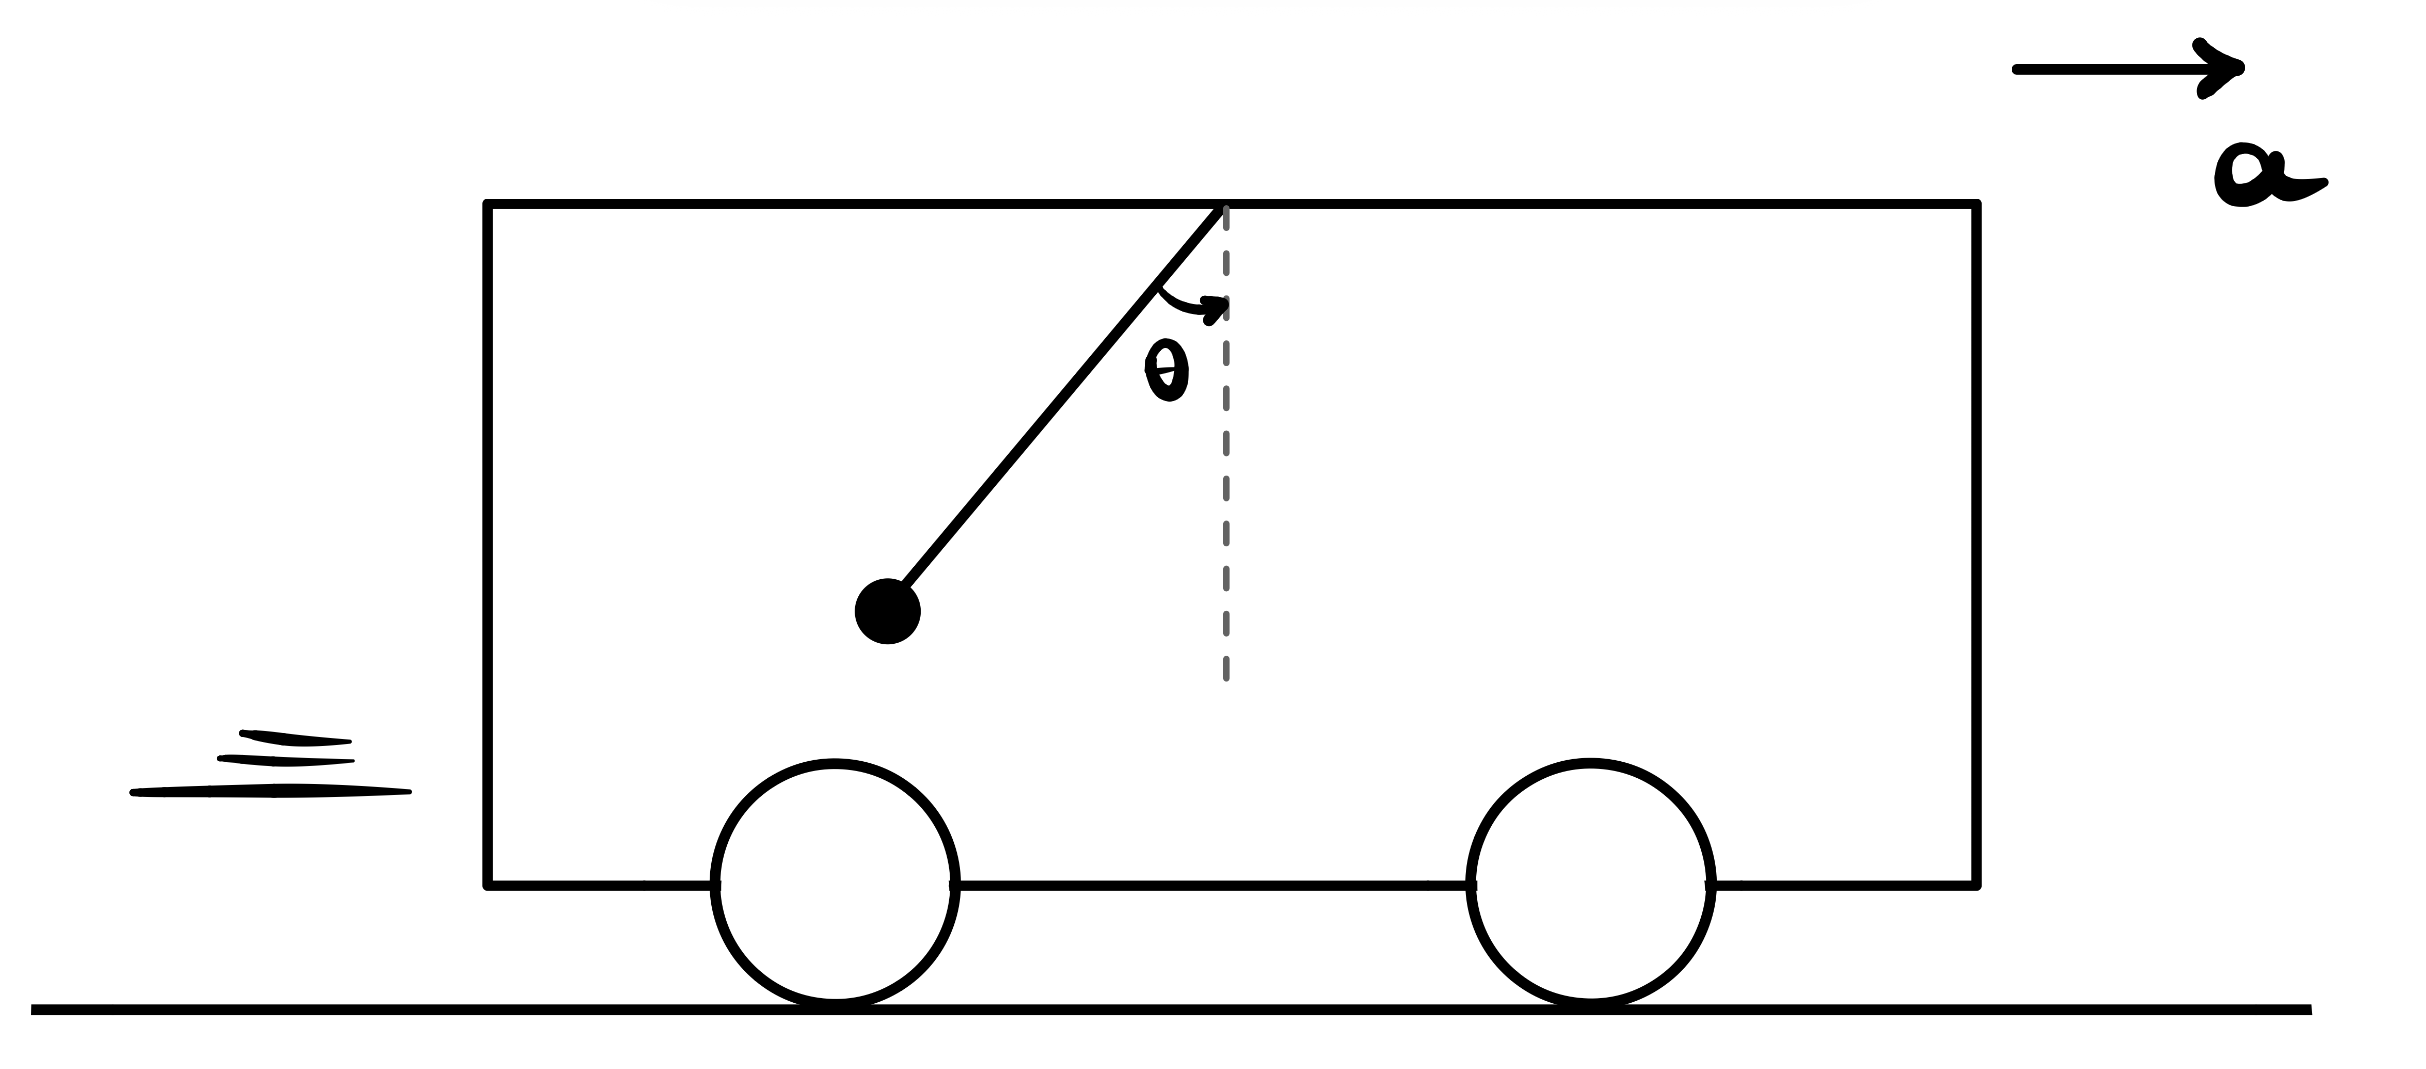
\includegraphics[width=0.5\linewidth]{imagensdinamicanewton/pendulodenewtonexemplo21.png}};
  \end{scope}
\end{tikzpicture}
\captionof{figure}{}
\label{fig_mec_pendulodenewtonexemplo21}
} 
\vspace{0.3cm}

\resolucao

Se o pêndulo permanece em repouso em relação ao vagão isso quer dizer que ele compartilha exatamente da mesma aceleração que o vagão. Lembre-se: o repouso é o movimento compartilhado. Dois corpos que executem exatamente o mesmo movimento terão a impressão de estarem em repouso um em relação ao outro. Assim, montamos o diagrama de forças na esfera do pêndulo, que aparece na Figura \ref{fig_mec_pendulodenewtonexemplo22}.

\vspace{0.3cm}
{
\centering
\begin{tikzpicture}
  \begin{scope}[blend mode=multiply]
    \node {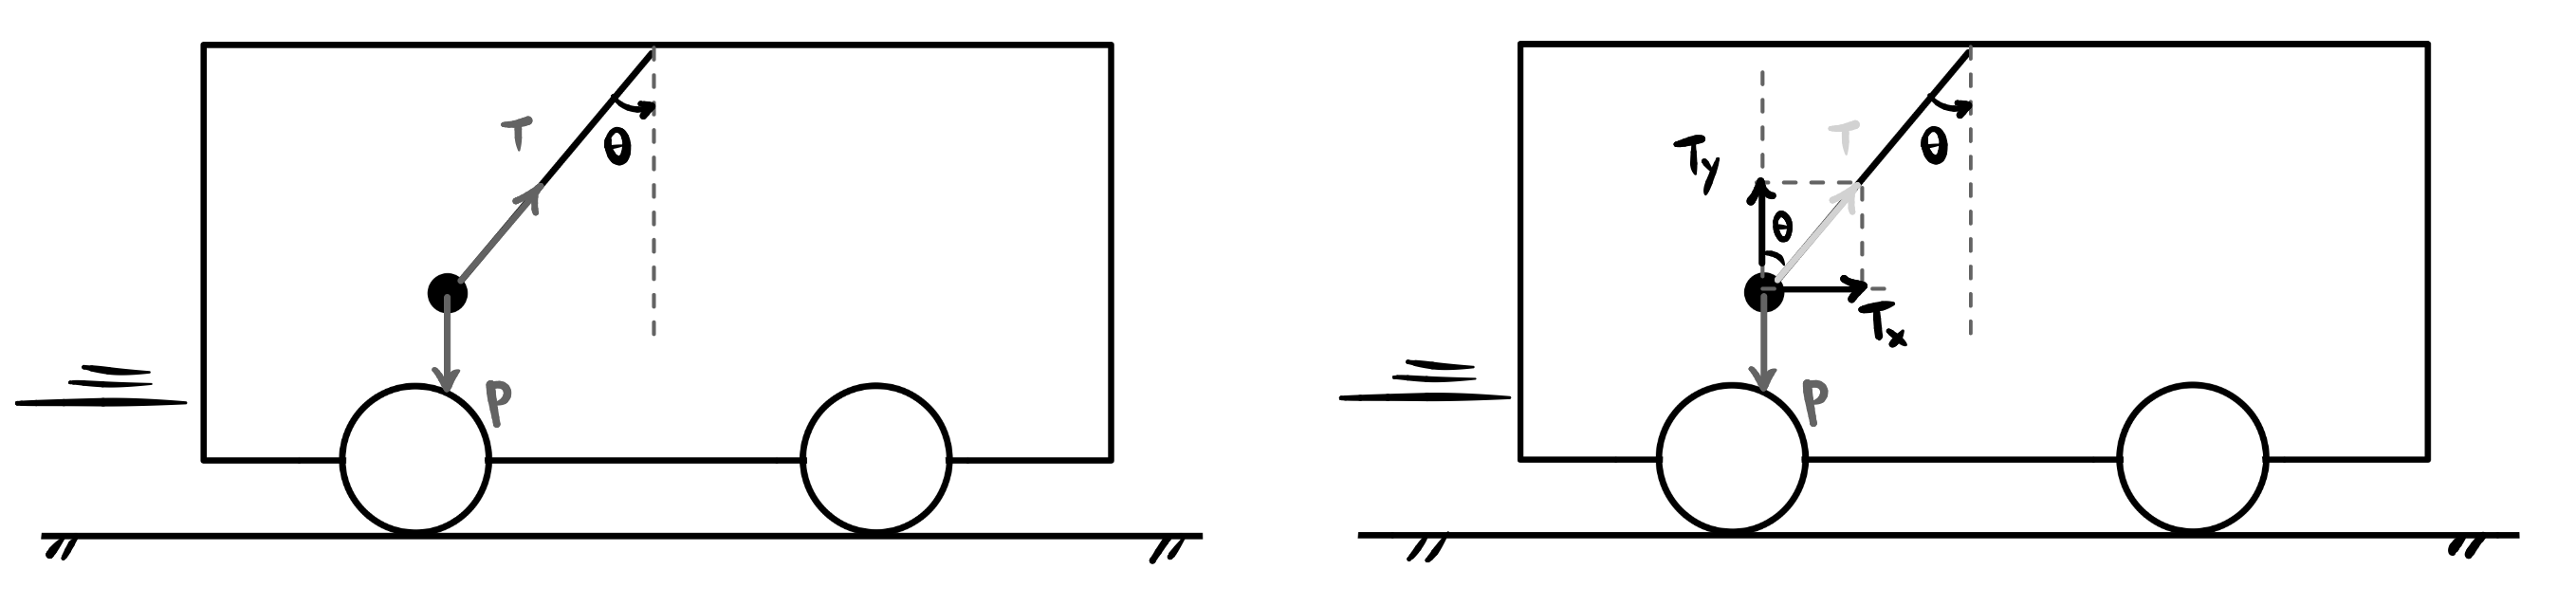
\includegraphics[width=0.99\linewidth]{imagensdinamicanewton/pendulodenewtonexemplo22.png}};
  \end{scope}
\end{tikzpicture}
\captionof{figure}{}
\label{fig_mec_pendulodenewtonexemplo22}
} 
\vspace{0.3cm}



Na vertical, como o vagão não se move, o pêndulo também não pode se mover. Logo, teremos:

$$ F_{\text{R}_y} = 0 \implies T_y = P \implies \boxed{T \cos \theta = mg.}$$

Na horizontal a resultante das forças deve produzir na massa a mesma aceleração $a$ que o vagão possui:

$$ F_{\text{R}_x} = m a_x \implies  \boxed{T \sin \theta =  ma.}$$

Dividindo as duas últimas equações seremos levados a

$$ \dfrac{\cancel T \sin \theta }{\cancel T \cos \theta } = \dfrac{\cancel ma}{\cancel mg} \implies \boxed{a = g \tan \theta.}$$

Logo, a aceleração do bloco deve ser exatamente igual a $a = g \tan \theta.$ Note que, para $\theta = 0,$ teremos $a=0.$ Ou seja, o pêndulo só fica alinhado com a vertical caso o vagão esteja em repouso ou em MRU -- as duas condições em que $a=0.$ Para que o pêndulo ficasse alinhado com a horizontal, isto é, $\theta = \sfrac{\pi}{2},$ seria preciso ter $a \to \infty.$ Isso mostra que quando mais intensa é a aceleração, mais próximo da horizontal o pêndulo fica, tendendo à horizontal para uma aceleração infinitamente grande. 

\end{exemplo}

\vspace{0.3cm}


\begin{exemplo}[Nível III]\label{exemplo_dinamicanewton_p=mg03}

Uma sonda espacial pousa num planeta sem atmosfera. O astronauta realiza
o seguinte experimento: arremessa verticalmente para cima um objeto de
massa $m$, a partir do solo, com velocidade inicial $v_0$
desconhecida. Duas grandezas são medidas com precisão:

\begin{itemize}
  \item altura máxima atingida pelo objeto acima do solo: $H$;
  \item tempo total de voo (do lançamento até o retorno ao solo): $T$.
\end{itemize}

\noindent Determine:

\begin{enumerate}
  \item [a)] o valor de $g$ naquele planeta, em função de $H$ e $T$;
  \item [b)] a velocidade inicial $v_0$ do lançamento, em função de $g$ e $T$;
  \item [c)] o peso do objeto nesse planeta, em função de $m$, $H$ e $T$;
  \item [d)] se o astronauta tivesse medido apenas $T$, sem registrar $H$,
  seria possível determinar $g$? Justifique.
\end{enumerate}

\resolucao



\noindent\textit{a)} Tomamos o eixo positivo para cima e a origem no solo. O objeto é
lançado com $v_0 > 0$ e sofre aceleração $-g$ (gravidade para baixo)
durante todo o voo. O problema se divide em duas etapas de cálculo:

\begin{enumerate}
    \item [(i)] Equação de Torricelli para cálculo da altura máxima:
    \begin{equation}
      0 = v_0^2 - 2gH \;\Longrightarrow\; v_0^2 = 2gH.  
      \label{eq_dinamicanewton_eqintermediariaexemplopeson31}
    \end{equation}
   



    \item [(ii)] Cálculo do tempo total de voo.

Como o movimento é simétrico (mesma aceleração constante, mesmo ponto
de partida e chegada, sem atrito), o tempo de subida é igual ao tempo
de descida. Portanto $T = 2\,t_{\text{sub}}$, onde $t_{\text{sub}}$ é
o tempo até a altura máxima. No ponto mais alto, $v = 0$, e da equação
$v = v_0 + at$ produz:

\begin{equation}
      0 = v_0 - g\,t_{\text{sub}}
  \;\Longrightarrow\;
  t_{\text{sub}} = \frac{v_0}{g}
  \;\Longrightarrow\;
  T = \frac{2v_0}{g}.
  \label{eq_dinamicanewton_eqintermediariaexemplopeson32}
\end{equation}

\end{enumerate}


Da Equação \eqref{eq_dinamicanewton_eqintermediariaexemplopeson32}: $v_0 = \dfrac{gT}{2}$. Substituindo na Equação \eqref{eq_dinamicanewton_eqintermediariaexemplopeson31}:

\[
  \left(\frac{gT}{2}\right)^2 = 2gH
  \;\Longrightarrow\;
  \frac{g^2 T^2}{4} = 2gH
  \;\Longrightarrow\;
  \boxed{g = \frac{8H}{T^2}.}
\]

\medskip
\noindent\textit{b)} Com $g$ determinado, obtemos $v_0$ pela Equação \eqref{eq_dinamicanewton_eqintermediariaexemplopeson32}:

\[
  \boxed{v_0 = \frac{gT}{2} = \frac{4H}{T}.}
\]

\medskip
\noindent\textit{c)} O peso do objeto no planeta:

\[
  \boxed{P = mg = \frac{8mH}{T^2}.}
\]

\noindent O peso depende das duas medidas experimentais $H$ e $T$, e
cresce com $H$ (quanto mais alto o objeto sobe, mais forte é a
gravidade local)\footnote{Um pouco estranho este resultado, não? O leitor consegue perceber a razão de sê-lo?} e decresce com $T^2$ (quanto mais tempo o objeto
permanece no ar, mais fraca é a gravidade que o puxa de volta). O
objeto tem a mesma \emph{massa} $m$ em qualquer lugar do universo;
o que muda é o \emph{peso}, que é ditado pelo campo gravitacional
local.

\medskip
\noindent\textit{d)} Se apenas $T$ fosse conhecido, a equação
disponível seria $T = 2v_0/g$, ou seja:

\[
  \frac{v_0}{g} = \frac{T}{2}.
\]

\noindent Esta é uma relação entre duas incógnitas, não uma equação
que as determina individualmente. Há infinitas combinações de $g$ e
$v_0$ que satisfazem $v_0/g = T/2$ para um dado $T$: basta tomar
qualquer $g > 0$ e definir $v_0 = gT/2$. Sem a segunda medida $H$
--- ou qualquer outra informação independente --- o sistema é
indeterminado. Dois dados são necessários para determinar duas
incógnitas.



\end{exemplo}




\begin{secnivel}[Lei de Hooke]{I}{Lei de Hooke}
  
  \eqLdois{exp}{eq_dinamicanewton_leihooke}{F = kx}

\end{secnivel}







\secgfe{De onde vem} 

A lei de Hooke nos diz qual é a força $F$ exercida por uma mola de constante elástica $k$ quando deformada de $x$ em relação ao seu comprimento inicial. Como mostra a Figura \ref{fig_dinamicanewton_hooke01}, quando distendemos uma mola, a sua tendência natural é retornar à posição de equilíbrio. Sendo assim, manifesta-se nas extremidades da mola uma força que a puxa de volta para sua posição inicial.

\vspace{0.3cm}
{
\centering
\begin{tikzpicture}
  \begin{scope}[blend mode=multiply]
    \node {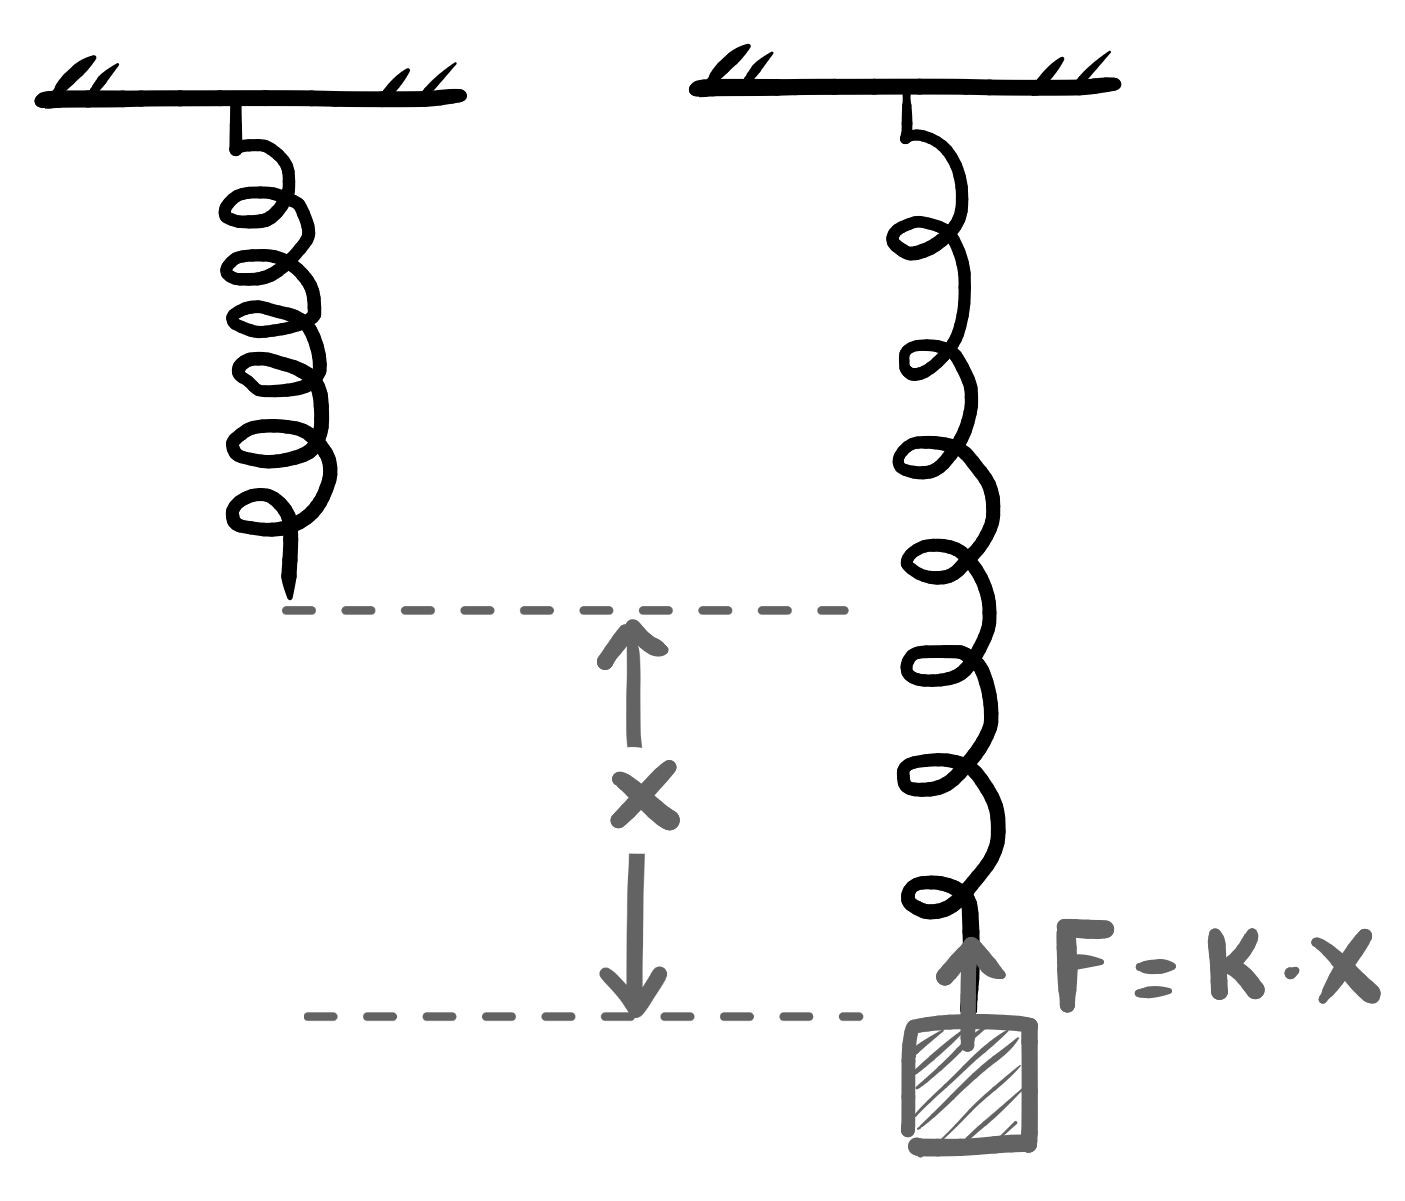
\includegraphics[width=0.3\linewidth]{imagensdinamicanewton/leihooke1.png}};
  \end{scope}
\end{tikzpicture}
\captionof{figure}{Ao ser distendida a mola tende a voltar para sua posição inicial. Com isso, surgem forças nas suas extremidades puxando-a de volta para sua posição natural.}
\label{fig_dinamicanewton_hooke01}
} 

\vspace{0.3cm}

A Equação \eqref{eq_dinamicanewton_leihooke} diz que tal força é diretamente proporcional à deformação $x$ da mola. Este é um fato obtido experimentalmente: para uma certa mola, pode-se avaliar, para diferentes deformações, qual é o valor da força que se manifesta em sua extremidade. Ao fazer isso, o experimento irá nos fornecer alguns dados, mostrados no gráfico da primeira imagem da Figura \ref{fig_dinamicanewton_hooke03}. Os dados experimentais indicam que a relação entre $F$ e $x$ é linear: uma relação de proporção direta, do tipo $y(x)=ax,$ ou, no nosso caso, $F(x)=kx.$

\vspace{0.3cm}
{
\centering
\begin{tikzpicture}
  \begin{scope}[blend mode=multiply]
    \node {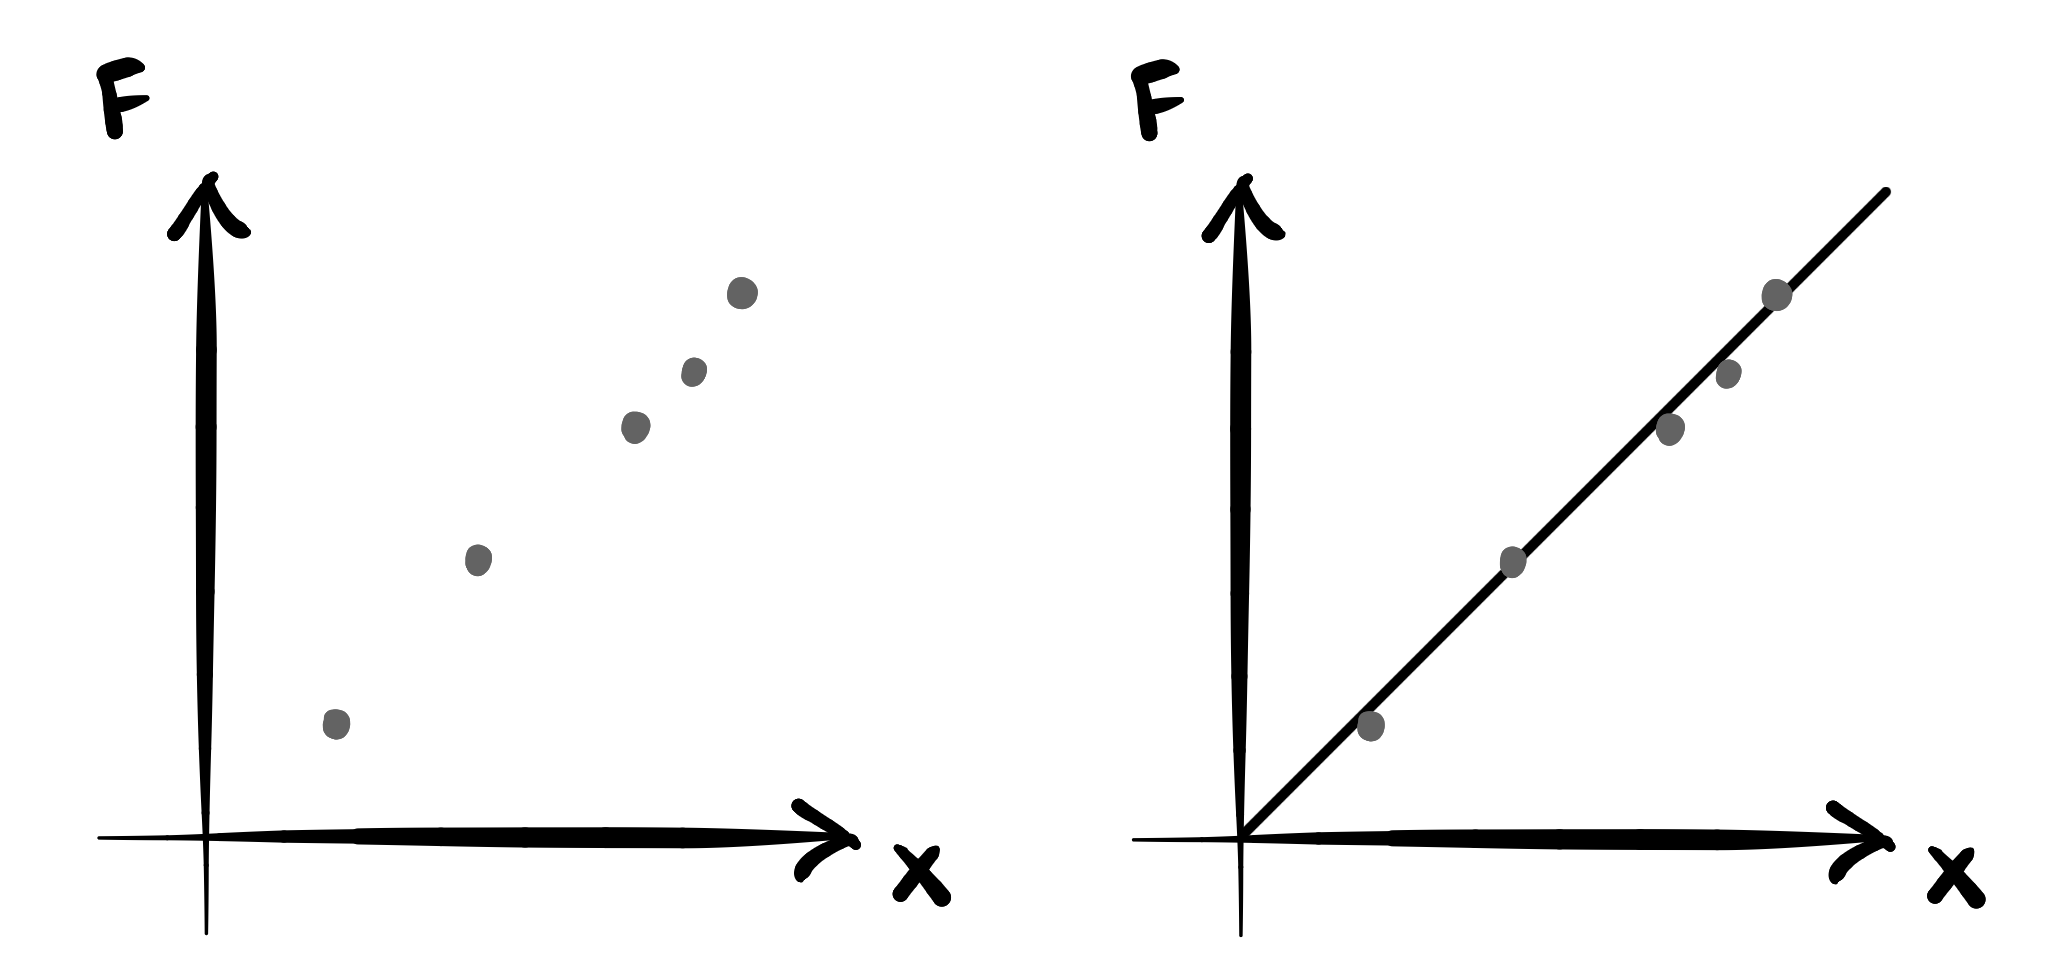
\includegraphics[width=0.5\linewidth]{imagensdinamicanewton/leihooke3.png}};
  \end{scope}
\end{tikzpicture}
\captionof{figure}{Ao plotar as forças $F$ que se manifestam na extremidade da mola para diferentes deformações $x$ encontramos que a relação entre essas duas grandezas é linear.}
\label{fig_dinamicanewton_hooke03}
}
\vspace{0.3cm}


É comum também, em algumas literaturas, apresentar a Equação \eqref{eq_dinamicanewton_leihooke} na forma $F=-kx.$ Neste caso, o sinal negativo entra ali apenas para indicar que a força terá sentido contrário ao deslocamento da mola. Como mostra a Figura \ref{fig_dinamicanewton_hooke01}, ao puxar a mola para baixo, a força elástica irá se manifestar para cima, puxando a mola de volta para sua posição inicial.




\secgfe{Onde é usada}

A Equação \eqref{eq_dinamicanewton_leihooke} será usada, naturalmente, em qualquer problema que envolva uma mola/elástico; como em um estilingue ou um arco e flecha. Cabe, contudo, trazermos luz ao leitor para alguns contextos em que as molas aparecem de forma implícita.

Um deles refere-se a um contexto bem interessante. Considere o seguinte: se a força peso de um corpo, como vimos na Equação \eqref{eq_dinamicanewton_peso=mg}, é a força de interação gravitacional entre a terra e o corpo, como podemos medi-la? A resposta a essa pergunta está relacionada a molas e à Equação \eqref{eq_dinamicanewton_leihooke}.

A Figura \ref{fig_dinamicanewton_hooke02} mostra, de forma simples, a estrutura de uma balança. Tal objeto funciona com um sistema de diversas pequenas molas -- simplificado por uma única mola na figura. Ao subir na balança, por conta da sua força peso, o indivíduo será puxado contra o chão, o que o fará empurrar a mola para baixo, comprimindo-a.

\vspace{0.3cm}
{
\centering
\begin{tikzpicture}
  \begin{scope}[blend mode=multiply]
    \node {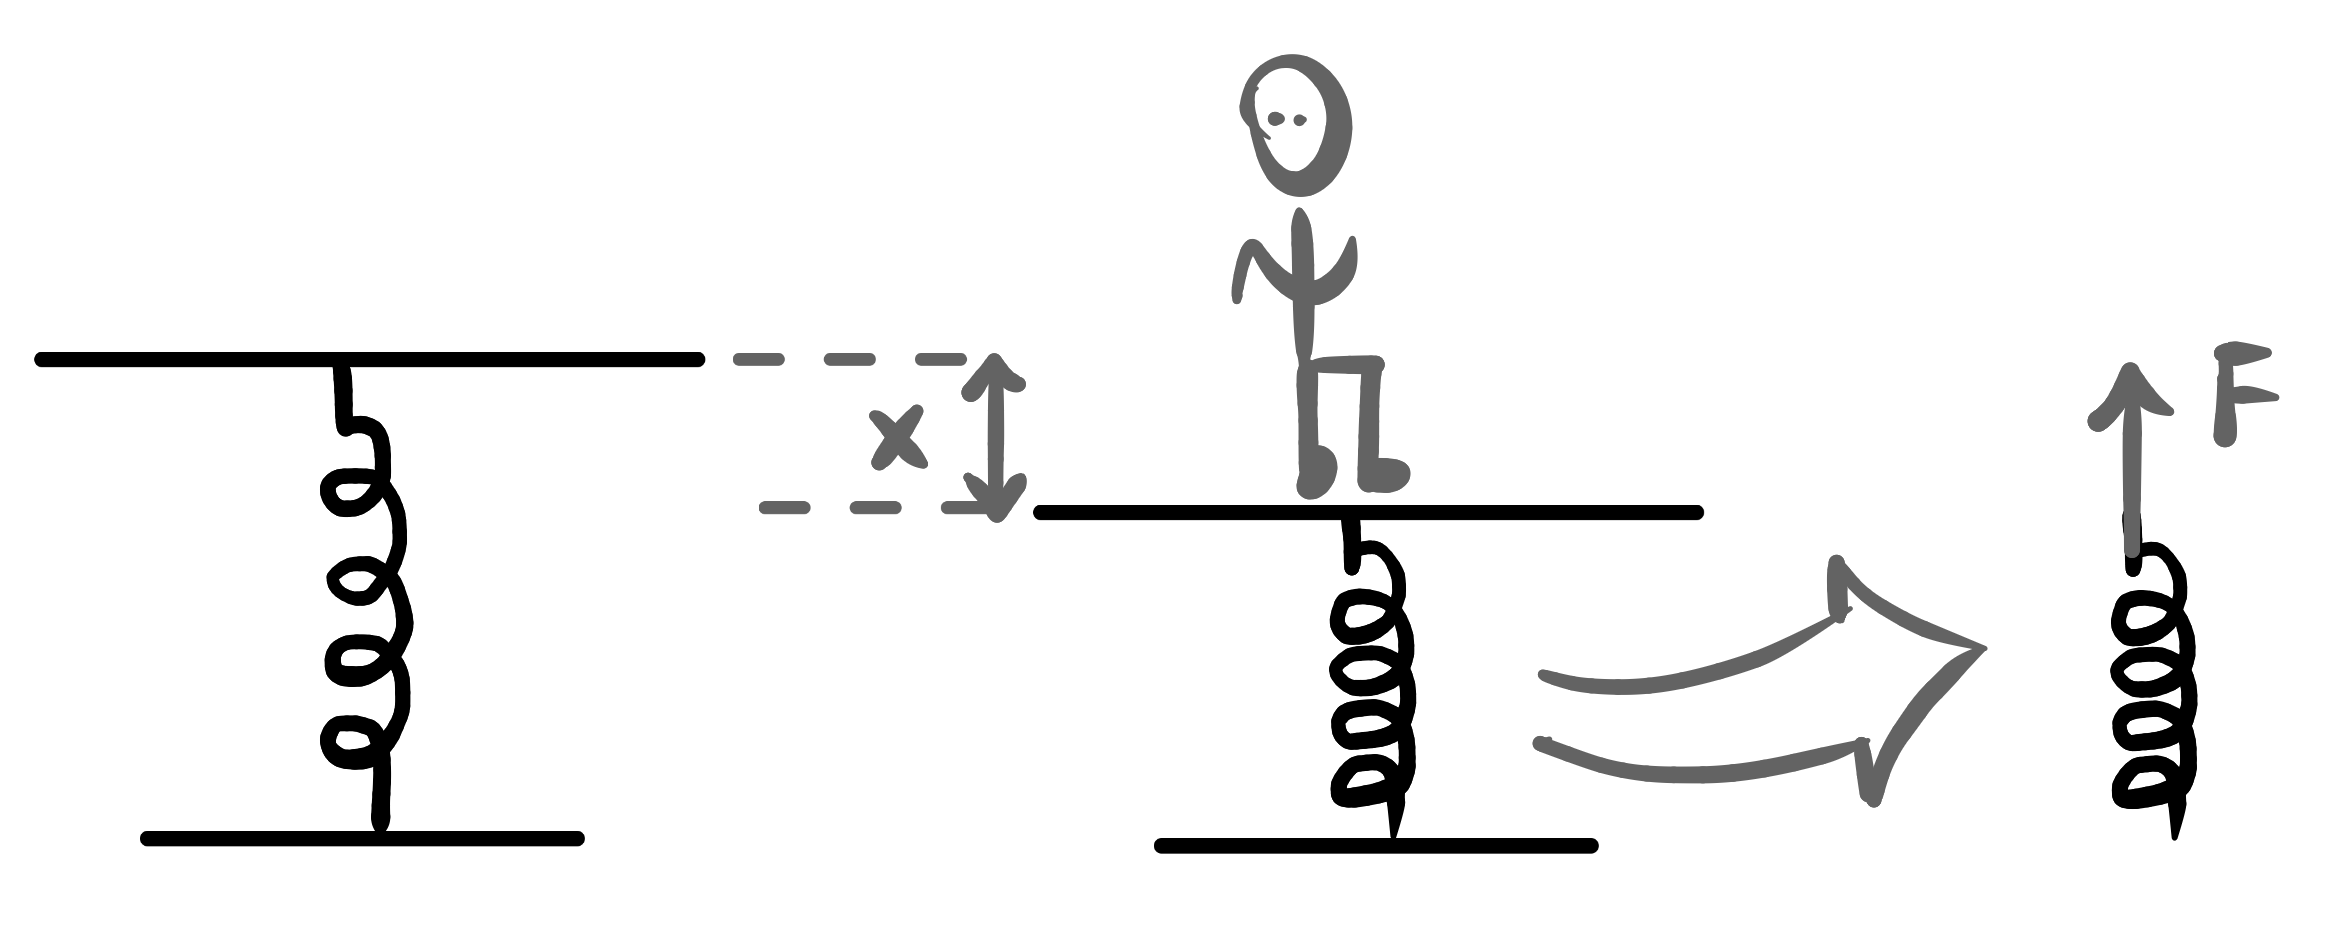
\includegraphics[width=0.5\linewidth]{imagensdinamicanewton/leihooke2.png}};
  \end{scope}
\end{tikzpicture}
\captionof{figure}{A balança não mede a sua força peso: ela mede o quanto as molas foram comprimidas.}
\label{fig_dinamicanewton_hooke02}
} 

\vspace{0.3cm}

Ao atingir sua nova posição de equilíbrio,\footnote{Situação em que a mola terá parado de ser comprimida, ou seja, a força elástica, empurrando o indivíduo para cima, terá que ser igual ao seu peso, que empurra a mola para baixo -- nessa situação cessa a deformação da mola.} a mola terá se deformado de um tanto $x,$ o que pode ser facilmente medido, como destaca a figura.

Ora, sabendo qual é a mola usada na construção da balança, saberemos qual é o valor da sua constante elástica $k,$ que é uma propriedade intrínseca da mola. Munidos desses valores, podemos usar a Lei de Hooke para encontrar o valor da força elástica:

$$ F = kx,$$

\noindent haja vista que o valor de $x$ foi medido e o valor de $k$ é conhecido. Logo, com isso, teremos a força elástica $F$ com que a mola empurra o indivíduo para cima. Ora, se o indivíduo está em equilíbrio, isto é, a mola não está mais sendo comprimida, isso significa que a força que o empurra para cima -- a força elástica -- deve ser exatamente igual, em módulo, ao valor do seu peso $P$, que é a força que o puxa para baixo: se as forças se anularem o menino não irá comprimir a mola para além da sua compressão atual. Assim, teremos:

$$ F=P,$$

\noindent e, como a força elástica $F$ pode ser medida, conseguimos, indiretamente, obter o peso do indivíduo. Como $P=mg,$ basta informar para o sistema eletrônico o valor da gravidade $g$ na superfície da Terra e programar o visor para pegar a força obtida e dividi-la por tal valor, de modo a obter a massa do indivíduo:

$$ P =mg \implies m = \dfrac{P}{g}.$$

Perceba como é engenhoso o sistema da balança, uma vez que

\begin{enumerate}
    \item [(i)] A balança não mede \textbf{nunca} o seu peso $P$. O que ela consegue medir é um comprimento geométrico: o quando a mola foi deformada. Munidos deste valor e conhecendo a constante elástica da mola, a Equação \eqref{eq_dinamicanewton_leihooke} nos permite obter a força elástica que a mola exerce, empurrando a base com o menino para cima, a fim de voltar à sua posição inicial. 

    Se, neste ponto, o sistema estiver em equilíbrio: o menino não está descendo, comprimindo mais a mola; nem subindo, então significa que a sua força peso que o puxa para baixo é igual à força elástica que o empurra para cima: $F=P.$ Logo, obtemos o valor da força peso do indivíduo, \textbf{de forma indireta: o que medimos de fato é uma deformação, que nos permite computar a força elástica na mola. Pelo fato de ela, neste contexto, ser igual ao peso, conseguimos obter o peso do indivíduo}.

    \item [(ii)] Ainda assim, no final, o que teríamos não é a massa do indivíduo, mas sim o valor do seu peso, que foi medido de forma indireta. Desse modo, seria necessário informar ao sistema da balança o valor da gravidade $g$ no local onde ela se encontra e programá-la para pegar o valor obtido e dividir por $g$, pois, pela Equação \eqref{eq_dinamicanewton_peso=mg}, a massa é a razão entre a força peso e a aceleração da gravidade: $m=\sfrac{P}{g}.$
\end{enumerate}



Perceba que esse tipo de mecanismo constitui uma nova ferramenta para medir forças: as forças podem ser medidas com base na deformação de molas. Digamos que queremos avaliar quem é mais forte: Aristóteles ($A)$ ou Bohr ($B$). Podemos pedir para que Aristóteles puxe uma mola, fixa em uma parede, por exemplo, com sua força máxima $F_A.$

Em seguida, pedimos que Bohr puxe um sistema com duas molas idênticas, uma ao lado da outra, com sua força máxima $F_B$. Se constatarmos que Bohr consegue gerar a mesma deformação que Aristóteles, podemos dizer que ele é duas vezes mais forte, uma vez que teve que distender duas molas para tal. Isto é, $F_B= 2F_A$, como mostra a Figura \ref{fig_dinamicanewton_hooke04}. Tal dispositivo é conhecido como dinamômetro e é usado para medir forças com base na lei de Hooke.

\vspace{0.3cm}

{
\centering
\begin{tikzpicture}
  \begin{scope}[blend mode=multiply]
    \node {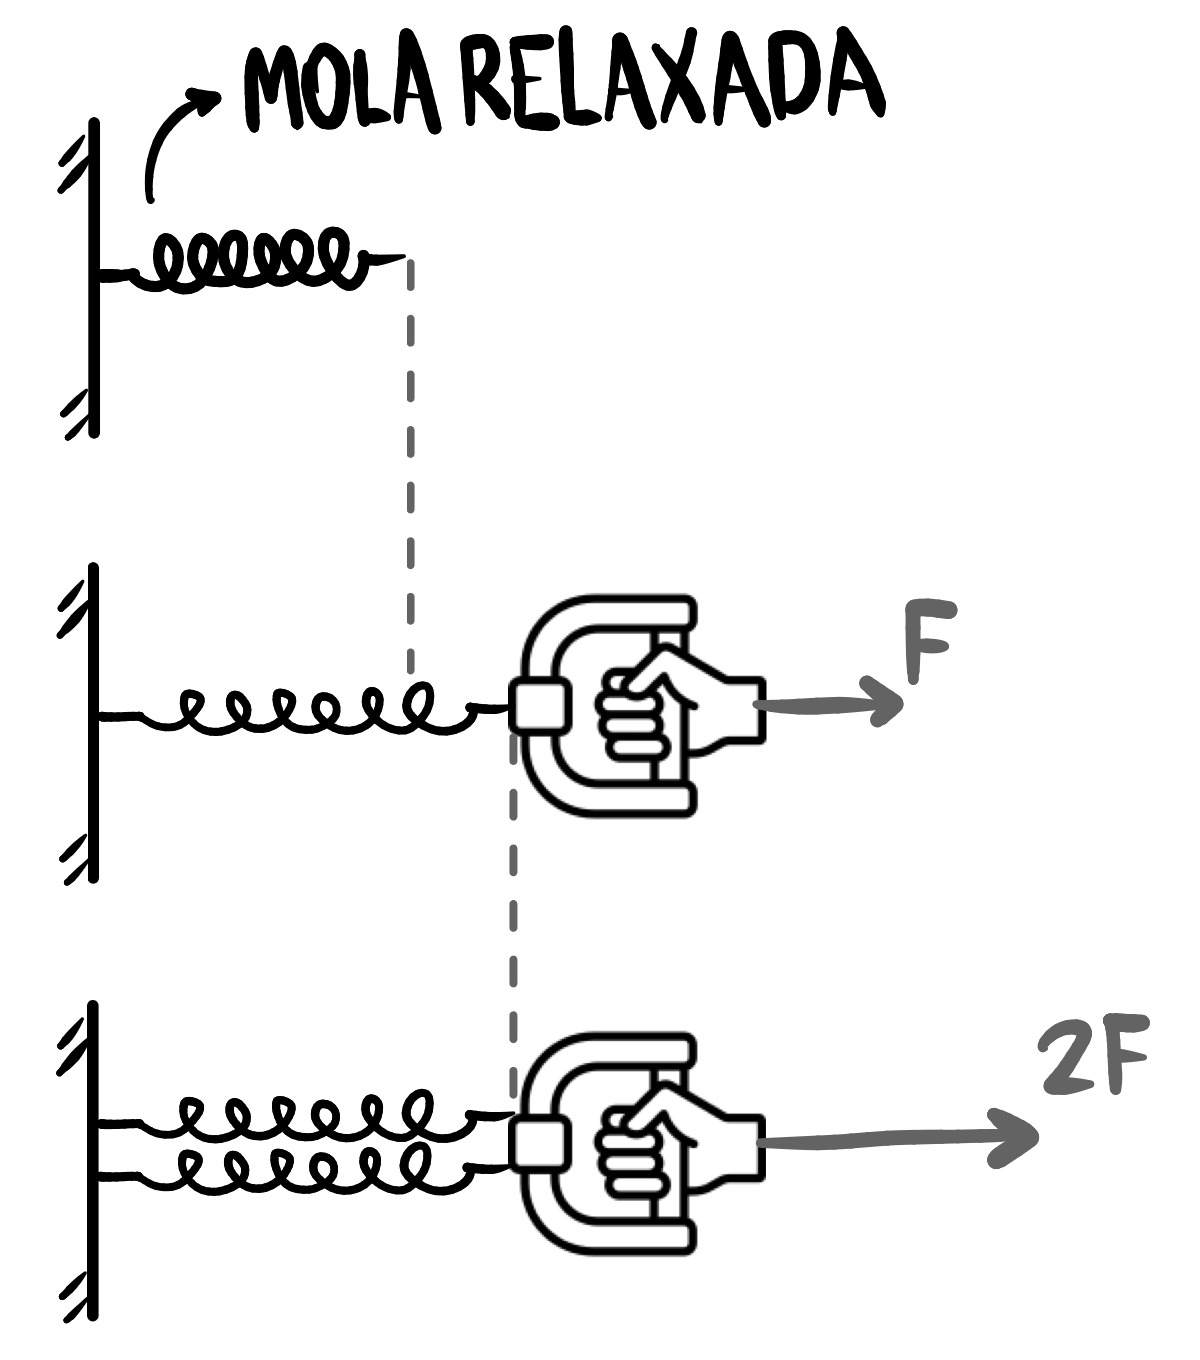
\includegraphics[width=0.35\linewidth]{imagensdinamicanewton/leihooke4.png}};
  \end{scope}
\end{tikzpicture}
\captionof{figure}{O mecanismo do dinamômetro.}
\label{fig_dinamicanewton_hooke04}
} 
\vspace{0.3cm}


\secgfe{Erros comuns}


Talvez o erro mais comum aqui seja confundir a deformação $x$ da mola com o seu comprimento natural $L.$ Se tivermos uma mola de constante elástica $k = 10$ N/cm, cujo comprimento natural -- isto é, o comprimento da mola relaxada, sem estar comprimida ou esticada -- é de 30 cm, qual é a força elástica se nós a esticarmos de $3$ cm? Alguns estudantes, neste caso, tendem a considerar como valor de $x$ para o cálculo na lei de Hooke o valor de 30 cm, ou de 33 cm. Contudo, o cálculo correto é

$$ F = kx = \dfrac{10 \text{ N}}{\text{ cm}} \cdot 3 \text{ cm} = 30 \text{ N.}$$

Perceba que o comprimento inicial da mola de 30 cm é irrelevante -- ele poderia ser de 50 cm, de 75 cm ou qualquer outro valor. O que importa para o cálculo da força elástica é a deformação $x$ da mola: o quanto ela foi esticada ou comprimida a partir da sua posição relaxada. Logo, o comprimento inicial $L$ da mola é irrelevante para o cálculo da força elástica.
 


\secgfe{Observações}

A constante $k$, chamada de constante elástica da mola, é uma grandeza que irá depender de características específicas daquela mola, nos dizendo quantos Newtons de força são necessários para deformar a mola de uma certa quantidade:

$$ [\text{k}] = \dfrac{[\text{F}]}{ [\text{x}]}  = \dfrac{\text{N}}{\text{m}}. $$

Uma mola de constante elástica $k = 80 \text{ N}/ $m é uma mola que exige 80 N de força para que ela seja esticada (ou comprimida) de exatamente 1 metro.


\vspace{0.3cm}

\begin{exemplo}[Nível I]\label{exemplo_newton_hooke01}

Considere a situação, como na Figura \ref{fig_dinamicanewton_hooke01}, que um bloco massa $m=4$ kg foi pendurado na extremidade de uma mola de constante elástica $k=50$ N/m.

Se o bloco fica em repouso após a distensão da mola, de quanto ela foi distendida?

\resolucao

No bloco atuam duas forças: o peso, verticalmente para baixo, e a força elástica, para cima. Se ele fica em repouso então as forças devem se anular:

$$ F_R = 0 \implies P = F \implies mg = kx \implies x = \dfrac{mg}{k}=\dfrac{4 \cdot 10}{50}= 0.8 \text{ m.}$$




\end{exemplo}



\vspace{0.3cm}

\begin{exemplo}[Nível II]\label{exemplo_newton_hooke02}

Um bloco de massa $m=5$ kg é amarrado na extremidade de uma mola. Ao empurrar o bloco 10 cm contra a parede, como mostra a Figura \ref{fig_dinamicanewton_hookeex021}, percebe-se que sua aceleração, assim que ele é solto, é de $2$ m/s$^2.$ Encontre a constante elástica da mola.




\vspace{0.3cm}
{
\centering
\begin{tikzpicture}
  \begin{scope}[blend mode=multiply]
    \node {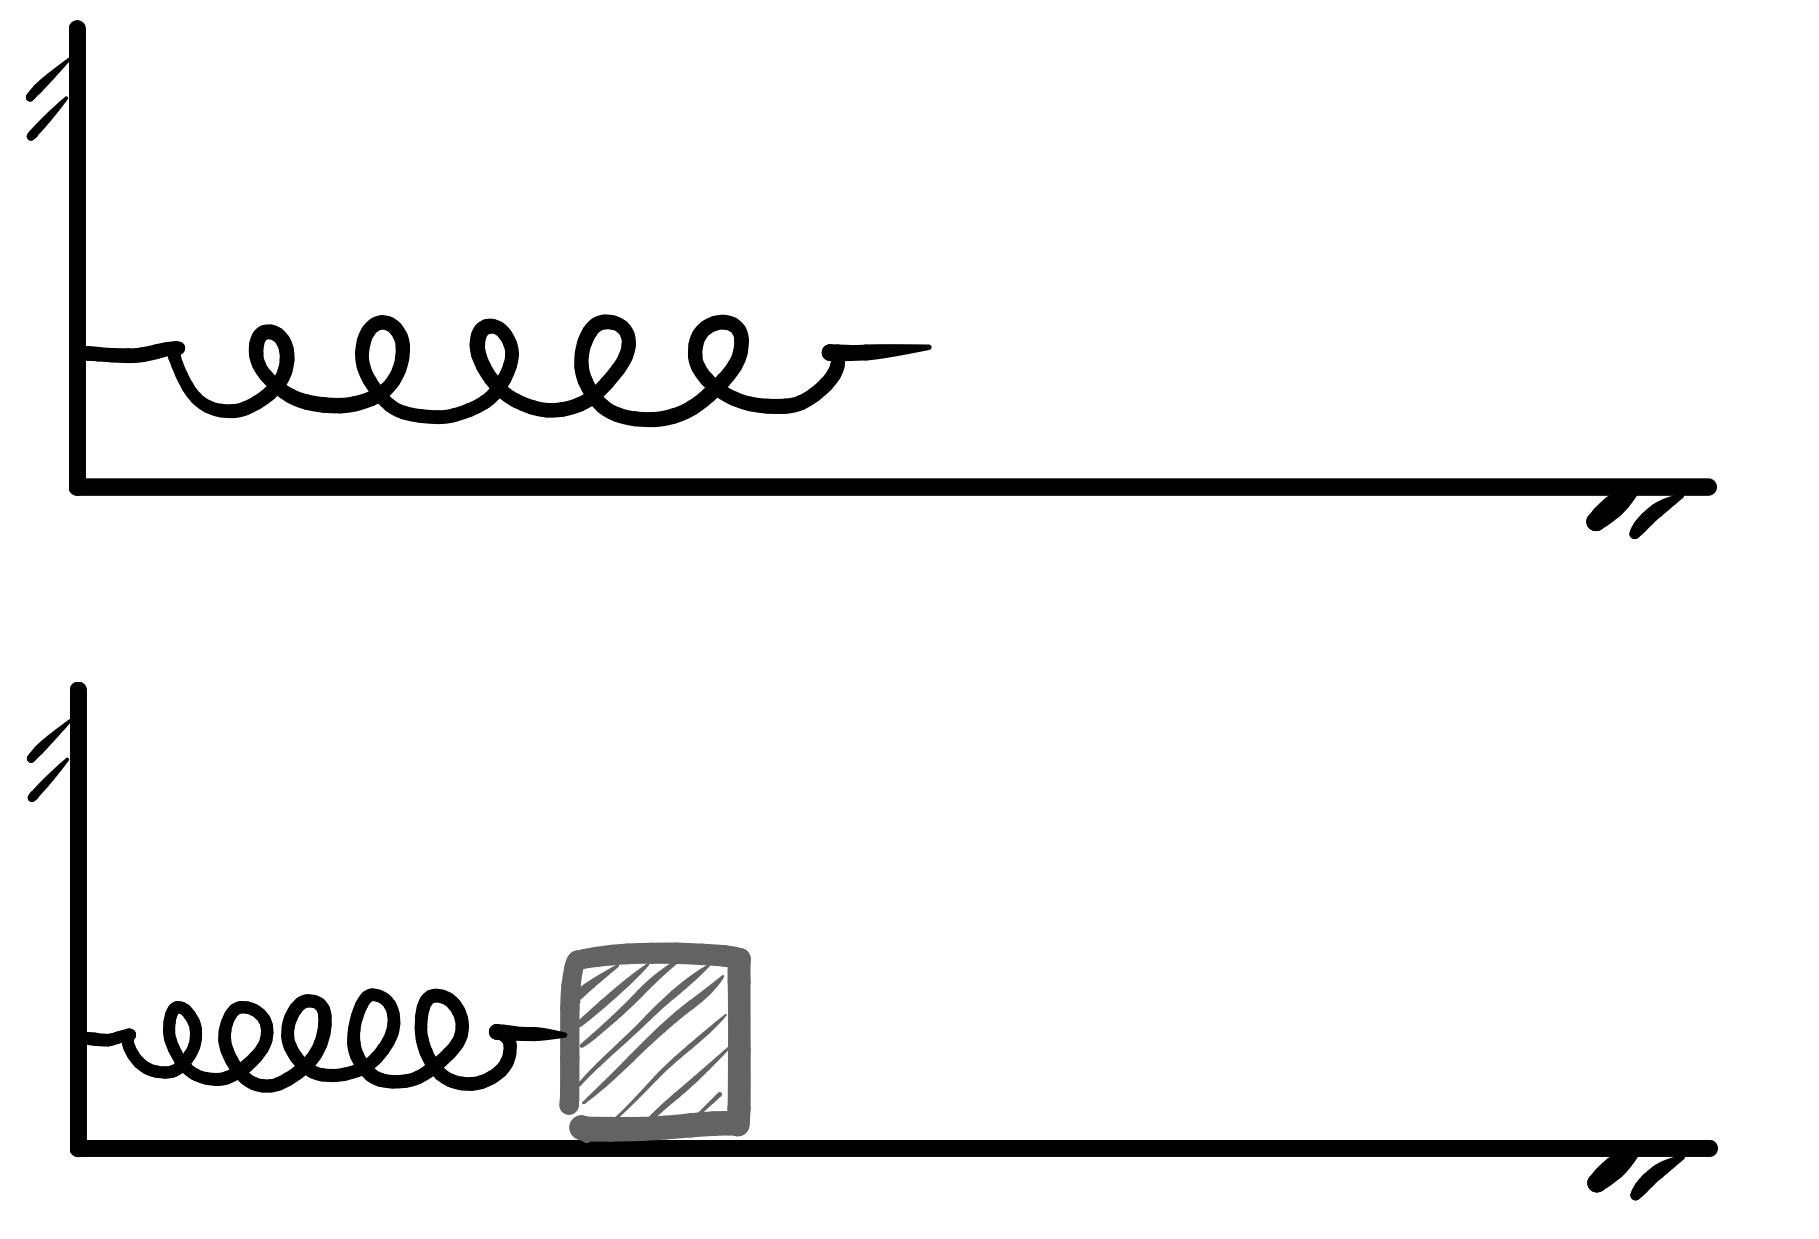
\includegraphics[width=0.35\linewidth]{imagensdinamicanewton/hookeex021.png}};
  \end{scope}
\end{tikzpicture}
\captionof{figure}{}
\label{fig_dinamicanewton_hookeex021}
} 
\vspace{0.3cm}


\resolucao

Como mostra a Figura \ref{fig_dinamicanewton_hookeex022}, analisando as forças na horizontal, a força resultante atuando no bloco será a própria força elástica. Logo, usando a lei de Hooke e a Segunda Lei de Newton, teremos

$$ F_R = F_{EL} \implies ma = kx \implies k = \dfrac{ma}{x} = \dfrac{5 \cdot 2}{0.1} = 100 \text{ N/m}.$$


\vspace{0.3cm}
{
\centering
\begin{tikzpicture}
  \begin{scope}[blend mode=multiply]
    \node {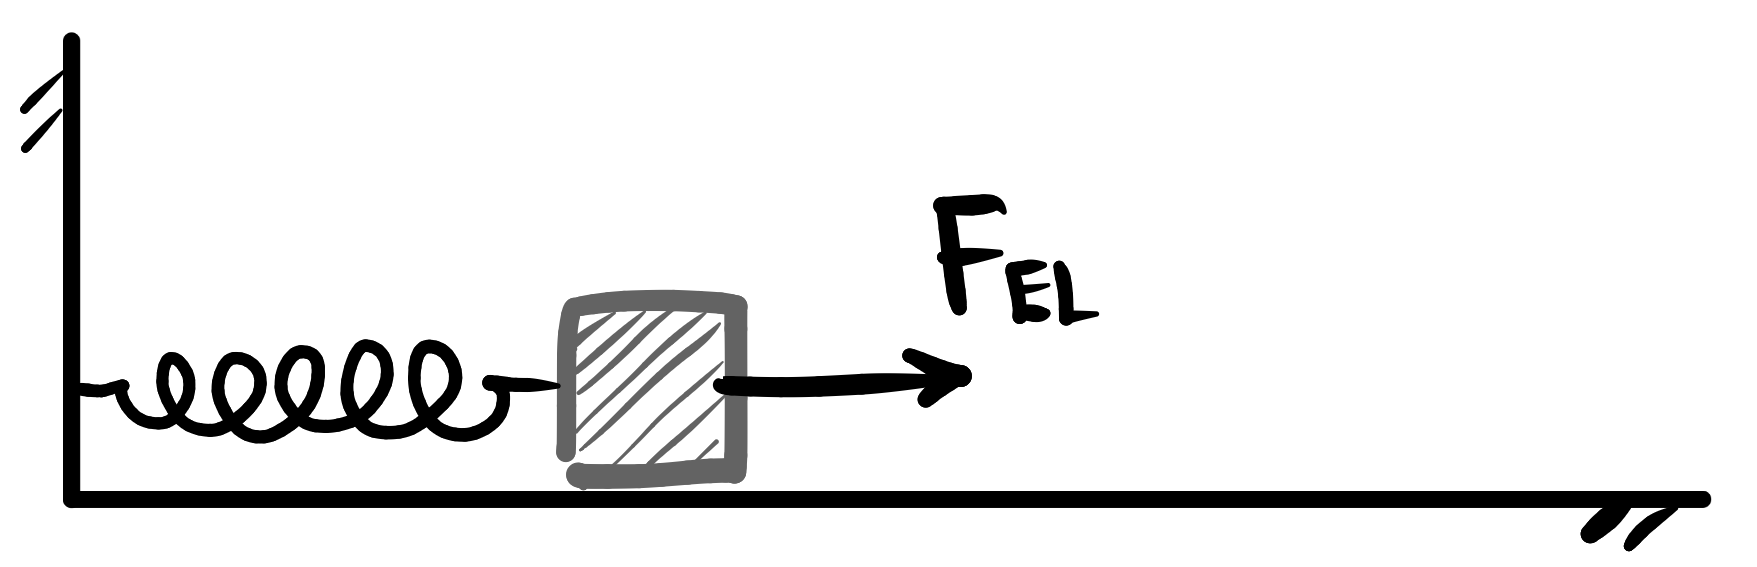
\includegraphics[width=0.35\linewidth]{imagensdinamicanewton/hookeex022.png}};
  \end{scope}
\end{tikzpicture}
\captionof{figure}{}
\label{fig_dinamicanewton_hookeex022}
} 
\vspace{0.3cm}

Note que convertemos a deformação $x$ da mola de centímetros para metros, a fim de inserir todas as informações na equação no SI e garantir que o resultado sairia, também, no SI.

\end{exemplo}


\vspace{0.3cm}



\begin{exemplo}[Nível III]\label{exemplo_newton_hooke03}

Considere duas molas de mesmo comprimento inicial e constantes elásticas $k_1$ e $k_2$. Mostre que

\begin{enumerate}
    \item [(a)] ao associar as molas em paralelo, isto é, de modo que a deformação delas seja a mesma, o sistema pode ser substituído por uma única mola de constante $k_{eq}=k_1+k_2.$

     \item [(b)] ao associar as molas em série, isto é, de modo que a força em cada uma delas seja a mesma, o sistema pode ser substituído por uma única mola de constante $k_{eq}$ dada por $\sfrac{1}{k_{eq}}= \sfrac{1}{k_1}+\sfrac{1}{k_2}.$
\end{enumerate}

\resolucao


\noindent a) Molas em paralelo — mesma deformação.

Quando as duas molas estão em paralelo, uma força externa $F$ é
aplicada ao sistema e ambas se deformam do mesmo valor $x$ (pois estão
fixadas nos mesmos dois pontos). Cada mola reage individualmente com
sua própria força:

\[
  F_1 = k_1\,x \qquad \text{e} \qquad F_2 = k_2\,x.
\]




\vspace{0.3cm}
{
\centering
\begin{tikzpicture}
  \begin{scope}[blend mode=multiply]
    \node {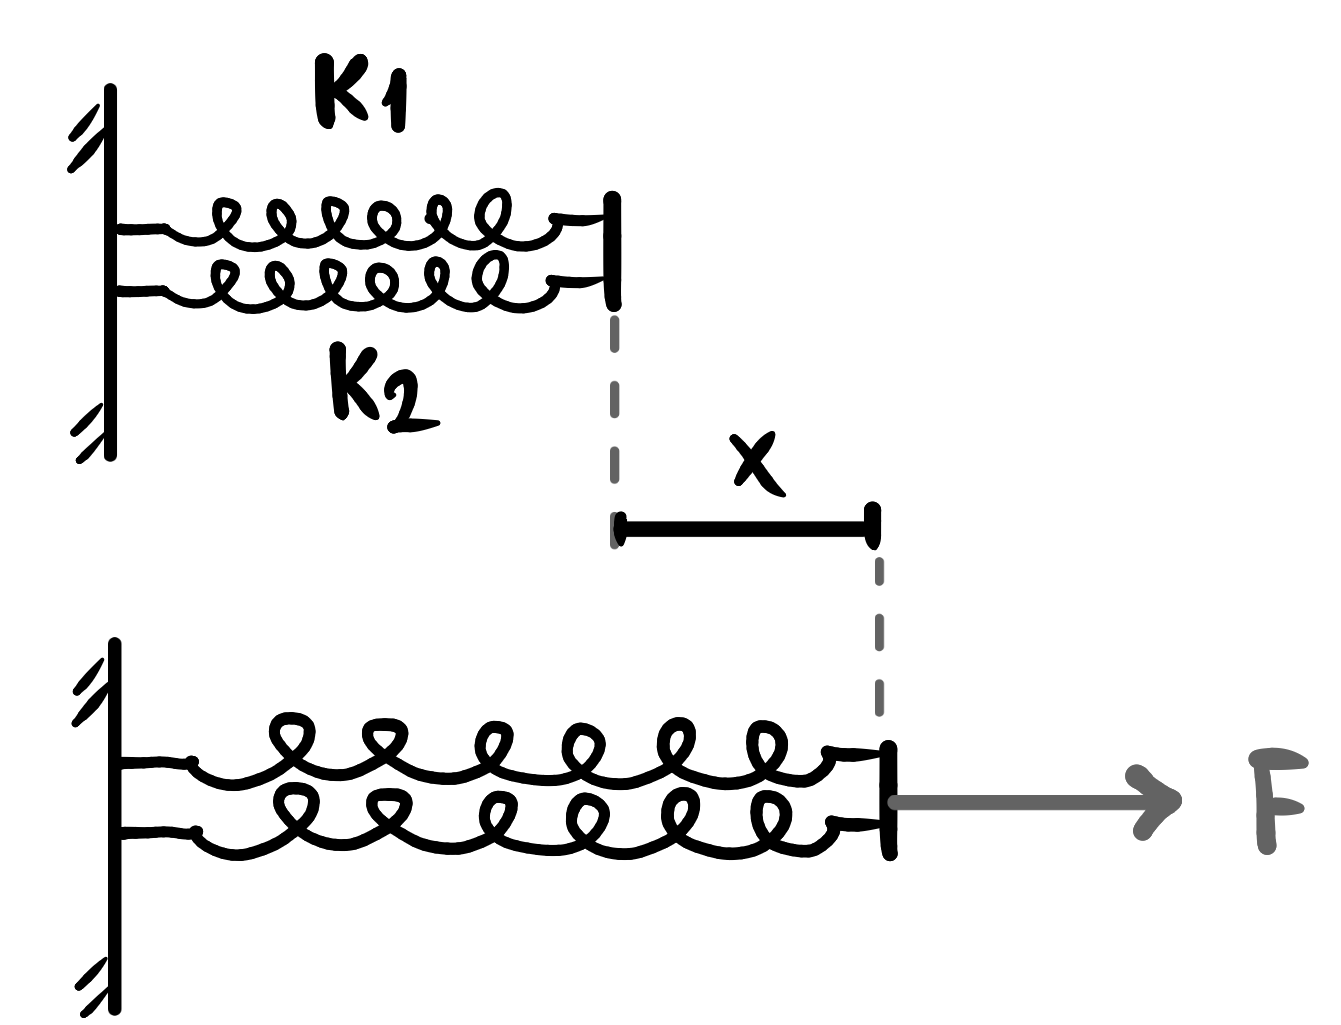
\includegraphics[width=0.40\linewidth]{imagensdinamicanewton/associacaodemolas1.png}};
  \end{scope}
\end{tikzpicture}
\captionof{figure}{Associação de molas em paralelo.}
\label{fig_dinamicanewton_associacaodemolas1}
} 
\vspace{0.3cm}


\noindent A força total que as molas exercem deve ser capaz de anular a força externa $F$ para que a mola fique em equilíbrio naquela posição. Logo:

\[
  F = F_1 + F_2 = k_1\,x + k_2\,x = (k_1 + k_2)\,x.
\]

\noindent Uma mola equivalente, por definição, satisfaz $F = k_{eq}\,x$. Ou seja, quando submetida a uma mesma deformação $x$ que o conjunto das outras duas, ela faz a mesma força total $F$ feita pelo sistema. Comparando com a expressão acima:


$$ F = k_{eq}\,x = (k_1 + k_2)\,x,$$

\noindent de onde segue que 

\[
  \boxed{k_{eq} = k_1 + k_2.}
\]

\noindent O resultado é intuitivo: em paralelo, as molas ``somam
esforços'' para resistir à mesma deformação, de modo que o sistema é
mais rígido do que qualquer uma das molas individualmente. Assim, podemos substituir o sistema de duas molas da Figura \ref{fig_dinamicanewton_associacaodemolas1} por uma única mola, de constante elástica $k_{eq} = (k_1 + k_2)$, e, quando submetida àquela mesma força $F,$ nossa mola sofrerá a mesma deformação $x$ que o sistema inicial sofria.

\bigskip
\noindent b) Molas em série — mesma força.

Quando as molas estão em série, a mesma força $F$ percorre toda a
cadeia --- se assim não fosse, algum trecho do sistema estaria
acelerando, o que contraria o equilíbrio estático. 

\vspace{0.3cm}
{
\centering
\begin{tikzpicture}
  \begin{scope}[blend mode=multiply]
    \node {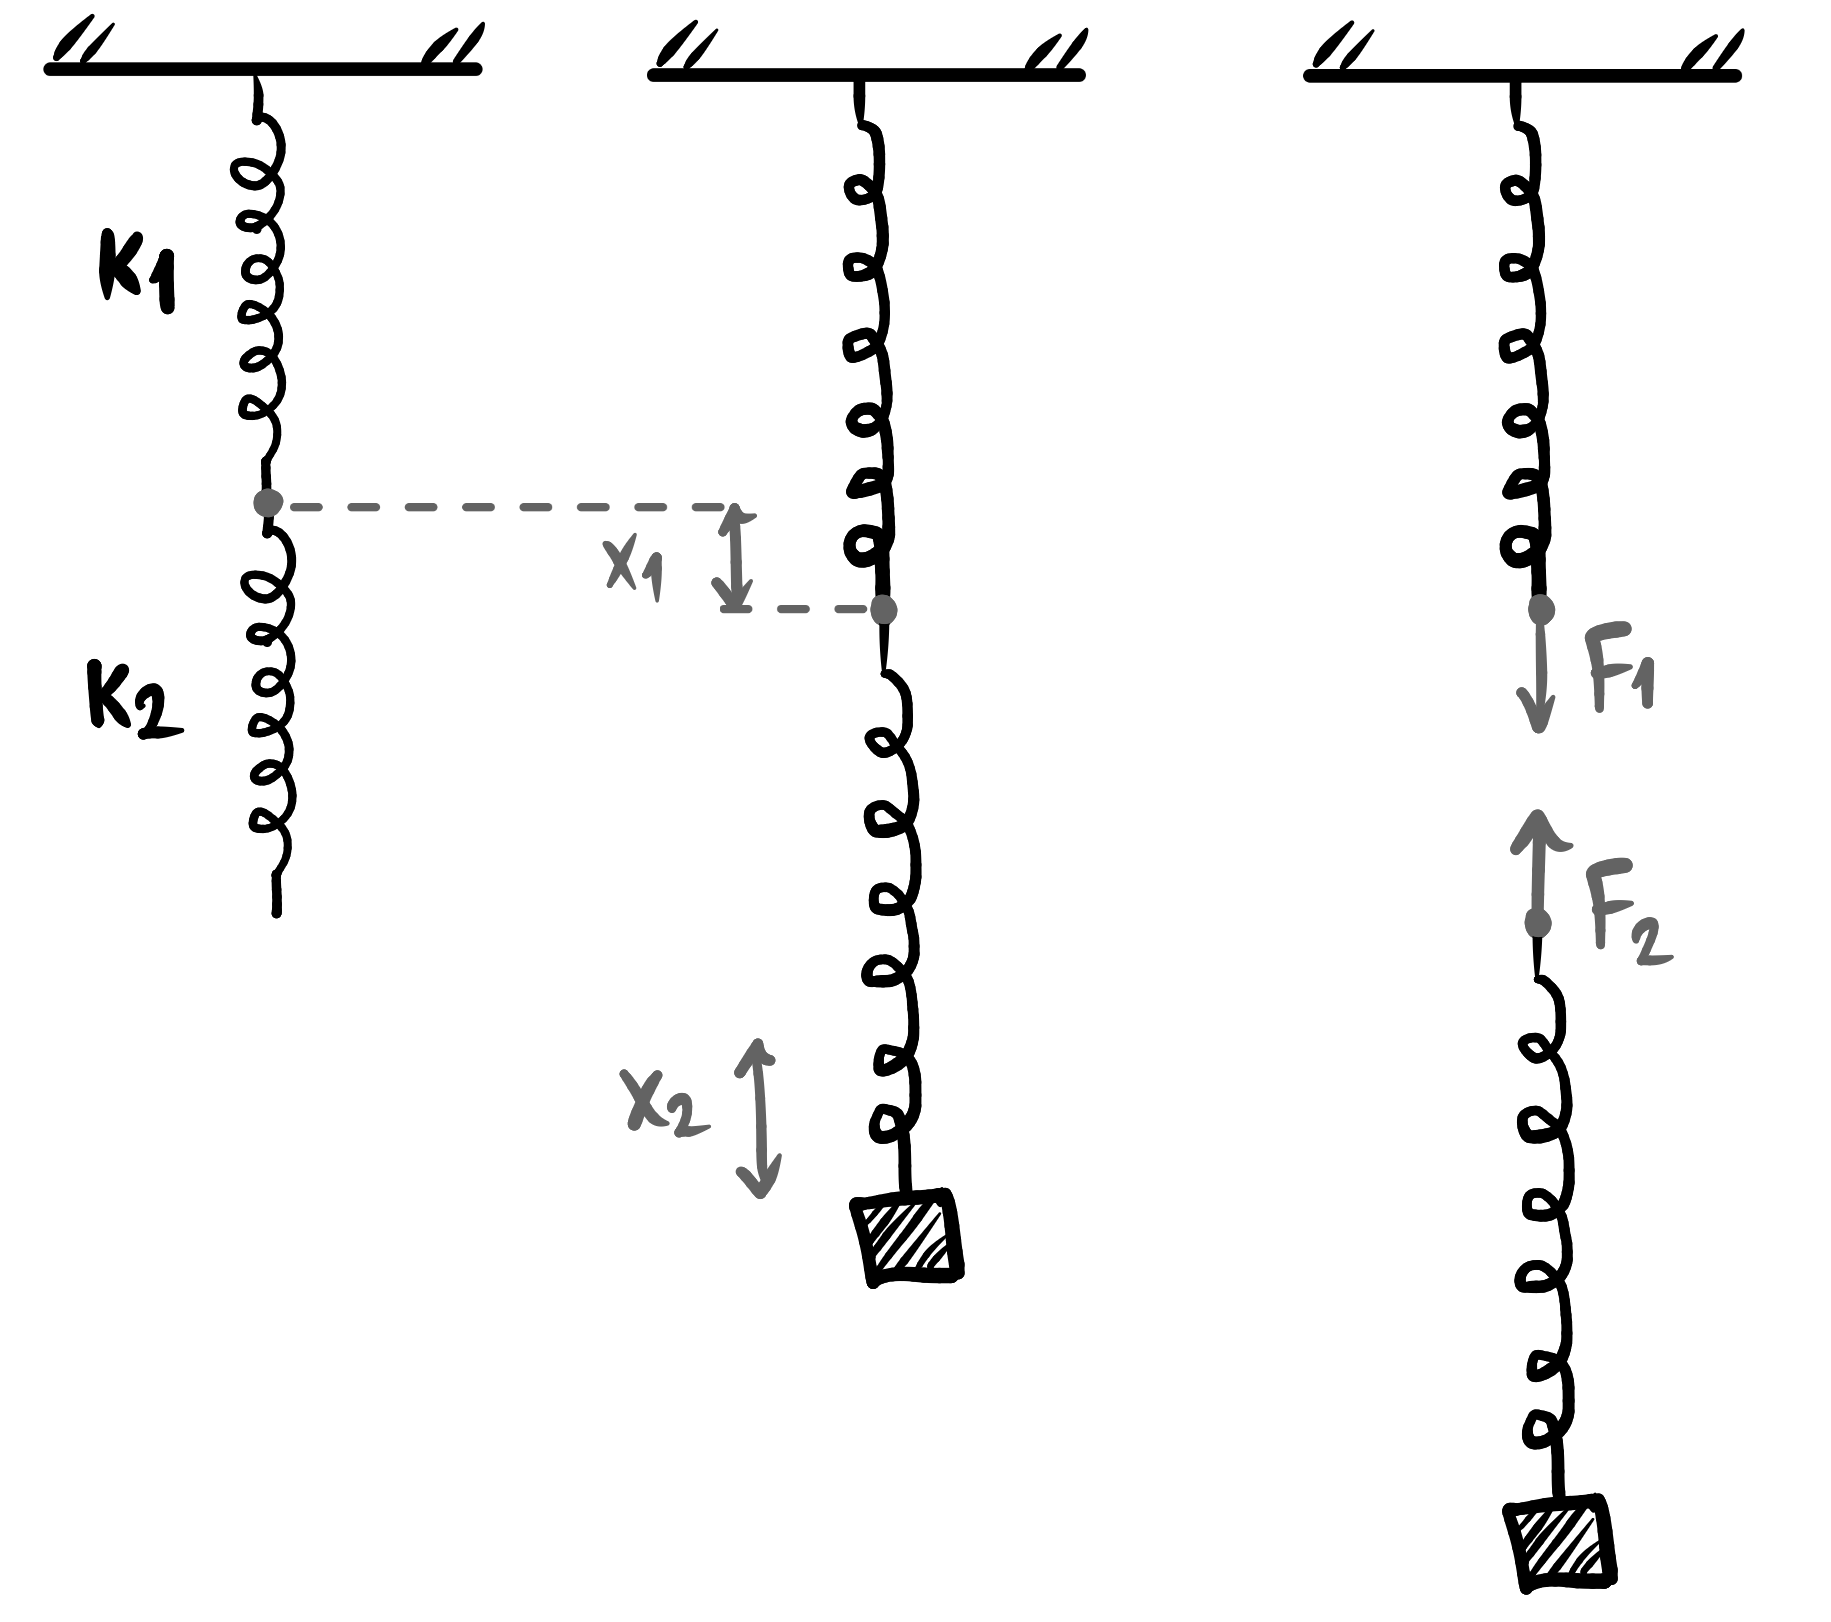
\includegraphics[width=0.55\linewidth]{imagensdinamicanewton/associacaodemolas2.png}};
  \end{scope}
\end{tikzpicture}
\captionof{figure}{Associação de molas em série.}
\label{fig_dinamicanewton_associacaodemolas2}
} 
\vspace{0.3cm}

A terceira imagem da Figura \ref{fig_dinamicanewton_associacaodemolas2} ilustra isso: a força $F_1$ com que a mola 1 puxa a mola 2, no ponto de junção, deve ser igual à força $F_2$ com que a mola 2 puxa a mola 1, para que o sistema não esteja acelerado naquele ponto. Logo:

$$ F_1 = F_2 = F\implies k_1 x_1 = k_2x_2 = F \implies \boxed{x_1 = \dfrac{F}{k_1} \quad \text{ e } \quad x_2 = \dfrac{F}{k_2}.}$$


\noindent A deformação total do sistema é a soma das deformações
individuais (as molas estão encadeadas, portanto seus alongamentos se
acumulam):

\[
  x = x_1 + x_2 = \frac{F}{k_1} + \frac{F}{k_2}
    = F\!\left(\frac{1}{k_1} + \frac{1}{k_2}\right).
\]

\noindent A mola equivalente é aquela que, submetida à mesma força $F$, produz a mesma deformação $x$ (ou, quando deformada do mesmo tanto $x$, produz a mesma força resistiva $F$). Logo, ela satisfaz $x = F/k_{eq}$, e, portanto:

$$ x = F\!\left(\frac{1}{k_1} + \frac{1}{k_2}\right) = \dfrac{F}{k_{eq}} ,  $$

\noindent de onde segue que

\[
  \boxed{\frac{1}{k_{eq}} = \frac{1}{k_1} + \frac{1}{k_2}.}
\]

\noindent Isso quer dizer que podemos substituir o sistema da Figura \ref{fig_dinamicanewton_associacaodemolas2} por uma única mola de constante $k_{eq}$ dada pela expressão acima que, ao amarrar na extremidade dessa mola a mesma massa que amarrou-se na extremidade da mola 2, a mola equivalente sofrerá a mesma deformação total $x=x_1+x_2$ do sistema original, proporcionando a mesma força sentida pela caixa.

\noindent O resultado também é intuitivo, embora em sentido inverso
ao do paralelo --- e vale a pena entendê-lo com cuidado. Em série,
a mesma força $F$ obriga \emph{cada} mola a ceder separadamente:
$x_1 = F/k_1$ e $x_2 = F/k_2$. O ponto de aplicação da força se
desloca a soma $x_1 + x_2$, que é \emph{maior} do que qualquer uma
das deformações individualmente. Como a rigidez é definida por
$k = F/x$ --- força dividida pela deformação --- e o denominador
cresceu sem que o numerador mudasse, a constante equivalente é
necessariamente menor do que $k_1$ e menor do que $k_2$.

Uma imagem ajuda: imagine segurar uma corrente pelo extremo e
puxá-la. Cada elo cede um pouco. Adicionar elos à corrente não a
torna mais rígida --- ao contrário, torna-a mais longa e mais
``mole''. Molas em série funcionam exatamente assim: cada mola é
um elo, e o sistema inteiro é a corrente. Quanto mais molas em
série, maior a deformação total para a mesma força, e portanto menor
a constante equivalente.

\end{exemplo}





\begin{secnivel}[Terceira Lei de Newton]{I}{Terceira Lei de Newton}
  
  \eqLdois{exp}{eq_newton_terceiraleinewton}{\vec F_{AB} = - \vec F_{BA}}

\end{secnivel}




Essa equação é um princípio geral da mecânica, classificada aqui como uma equação do segundo tipo: uma equação experimental. \footnote{Na verdade, as três leis de Newton são os princípios que ele assume como verdadeiros para estruturar toda a sua teoria da dinâmica. Nenhuma delas veio, de forma completa, de um experimento único, e não podem também ser demonstradas. Desse modo, a Equação \eqref{eq_newton_terceiraleinewton} não é exatamente experimental: ela é inspirada em resultados experimentais, como veremos, mas ela é adotada e postulada como um princípio geral de como a natureza funciona. O Apêndice \ref{apendice-eqs-exp-vs-dem} explora melhor essa nuance.} Tal equação diz que a força $\vec F_{AB}$ que a partícula $A$ faz em $B$ é sempre igual e contrária à força $\vec F_{BA}$ que a partícula $B$ faz em $A.$ Ou, nas palavras do próprio Newton:

\begin{center}
    \textit{A toda ação há sempre uma reação oposta e igual; isto é, as ações de dois corpos um sobre o outro são sempre iguais e dirigidas em sentidos contrários.}
\end{center}

Logo, parte-se da \textbf{premissa de que as forças sempre vem aos pares: a toda ação existe uma reação igual e contrária.} Ou seja, se dois indivíduos brigam e um desfere um soco no rosto do outro, a terceira lei de Newton diz que a força com que a mão do indivíduo $A$ bate no rosto do indivíduo $B$ é exatamente a mesma com que o rosto do indivíduo $B$ bate na mão do indivíduo $A.$ 

É por isso que ao trocar socos sua mão pode ser gravemente machucada -- mesmo que seja você quem desfere o golpe, a mesma força com que você atinge o rosto do indivíduo será aquela com que o rosto do indivíduo atingirá a sua mão. Nesse sentido, do ponto de vista físico, toda briga é um empate. O fato de o estrago ser maior no rosto do que na mão é apenas um detalhe biológico.

\secgfe{De onde vem}


Considere o experimento da Figura \ref{fig_dinamicanewton_thirdlawmomento}, que mostra duas bolinhas idênticas, se movendo uma em direção à outra, com a mesma velocidade. 

\vspace{0.3cm}
{
\centering
\begin{tikzpicture}
  \begin{scope}[blend mode=multiply]
    \node {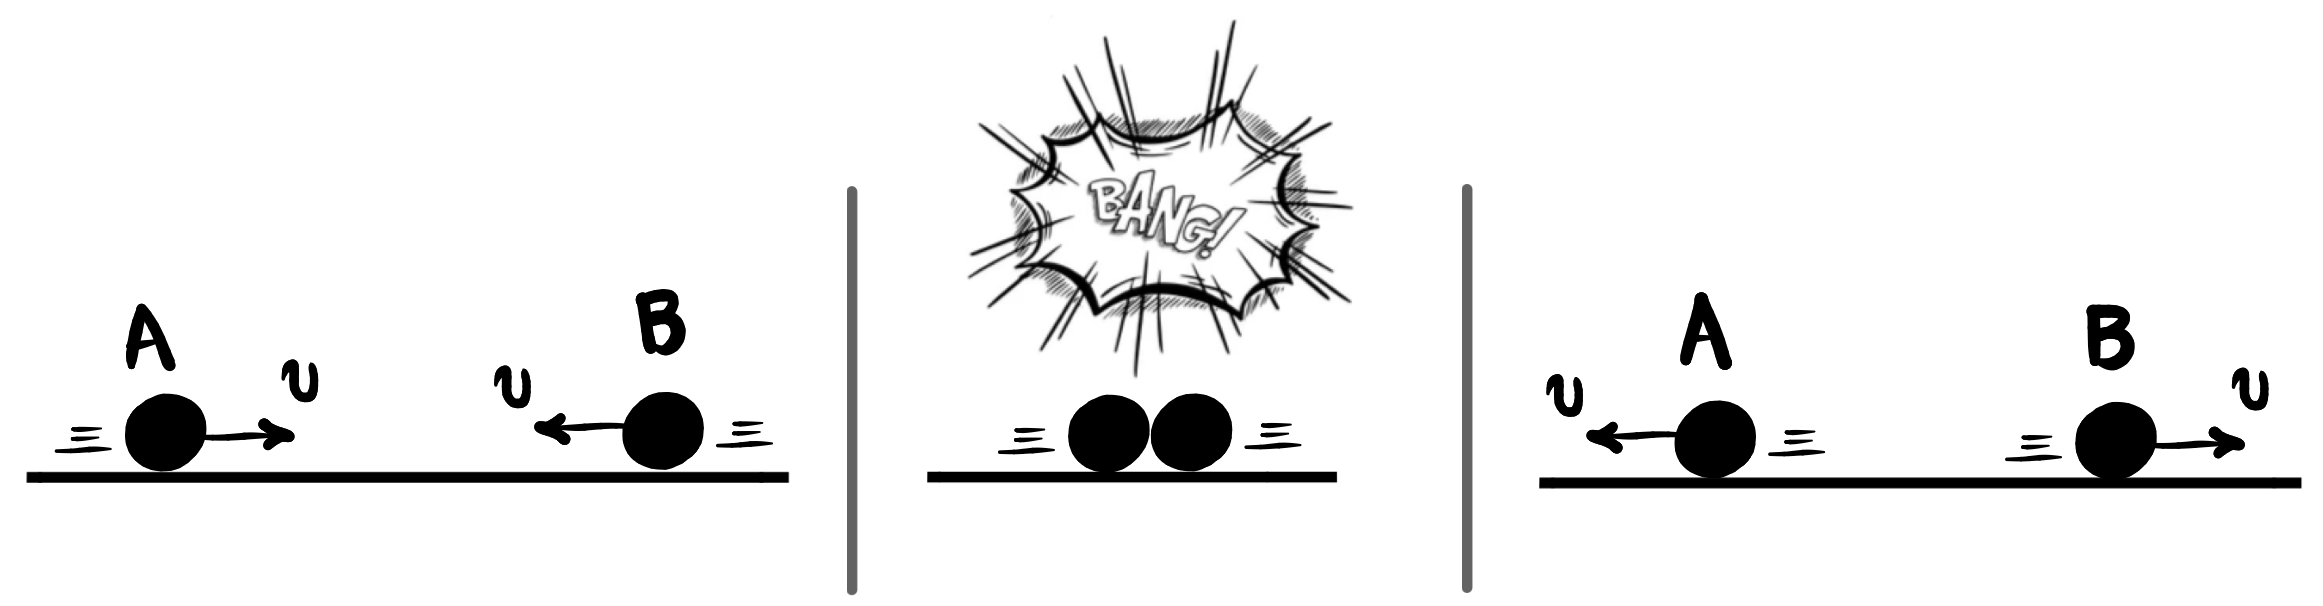
\includegraphics[width=0.8\linewidth]{imagensdinamicanewton/thirdlawnewton.png}};
  \end{scope}
\end{tikzpicture}
\captionof{figure}{Experimento de duas bolas, idênticas e de mesma velocidade, colidindo.}
\label{fig_dinamicanewton_thirdlawmomento}
} 
\vspace{0.3cm}

Ao fazer tal experimento, verifica-se que, após a colisão, as bolinhas mantêm o mesmo valor de velocidade, porém invertem o sentido do seu movimento. Ora, se houve variação do movimento (velocidade) então certamente houve aceleração. Mas a Segunda Lei de Newton diz que, para que haja aceleração, deve haver força resultante. Assim, a bolinha que inicialmente se movia para a direita deve ter sentido, durante a colisão uma força para a esquerda, de modo a variar seu movimento e inverter o sentido da sua velocidade. Já a bolinha que se movia para a esquerda deve ter sentido uma força para a direita, capaz de gerar uma aceleração e variar sua velocidade, de modo a inverter o sentido do seu movimento.

Dito isso, vemos que, durante este choque ideal, tudo indica que enquanto a bolinha $A$ bate na bolinha $B$, a bolinha $B$ também bate na bolinha $A.$ Ou seja, durante o choque, a bolinha $A$ faz uma força $F_{AB}$ na bolinha $B$, para a direita; porém a bolinha $B$ faz uma força -- no sentido contrário, para a esquerda -- $F_{BA}$ na bolinha $A.$

Ora, sendo as bolinhas idênticas (mesma massa) e tendo as duas sofrido exatamente a mesma variação de movimento (aceleração), as forças necessárias para que isso seja feito devem ser as mesmas, ou seja:

$$ F_{AB} = F_{BA},$$

\noindent o que, em palavras, quer dizer que a força com que a bolinha $A$ bate em $B$ tem exatamente o mesmo valor da força com que a bolinha $B$ bate em $A$.

Alguns estudantes costumam ter a curiosidade de saber qual é a ação e qual é a reação, mas isso é irrelevante e nem faz muito sentido. Seria o mesmo que perguntar: \textit{o que ocorreu primeiro, a bolinha $B$ bater em $A$ ou a bolinha $A$ bater em $B?$} Perceba que a pergunta não faz sentido porque as duas coisas ocorrem ao mesmo tempo: a colisão é um fenômeno único, e no mesmo instante em que $A$ faz a força $F_{AB}$ em $B,$ a bolinha $B$ faz a força $F_{BA}$ em $A.$ Ou seja, tanto faz quem é a ação e quem é a reação -- essa realmente é uma classificação que não tem importância alguma. O que importa é sempre o par ação-reação e o fato de que todas as forças sempre virão aos pares. Recapitulando, perceba que:

\begin{enumerate}
    \item [(i)] As forças $F_{AB}$ e $F_{BA}$ são de mesma natureza: forças de contato. Tais forças constituem um par ação-reação e, como neste caso, tal par sempre será constituído de forças de mesma natureza. Se a ação $F_{AB}$ for de natureza gravitacional, a reação $F_{BA}$ também será gravitacional. Se a ação for elétrica, a reação será também força elétrica, e por aí vai.
    
    \item [(ii)] As forças $F_{AB}$ e $F_{BA}$ atuam na mesma direção, possuem o mesmo valor porém sentidos contrários: a força $F_{AB}$ que $A$ faz em $B$ atua para a direita, enquanto a força $F_{BA}$ que $B$ faz em $A$ atua para a esquerda. Isso é exatamente o que está contido na relação vetorial da Equação \eqref{eq_newton_terceiraleinewton}.

    \item [(iii)] As forças $F_{AB}$ e $F_{BA}$ \textbf{atuam em corpos distintos: uma atua em $B$ e a outra em $A.$} Desse modo, um par ação-reação jamais irá se anular, justamente por atuarem em corpos distintos. 
    
    Não tem como a força peso que você está sentido agora se anular com a força peso que eu sinto, ainda que elas tenham o mesmo valor, mesma direção e sentidos contrários. Isso ocorre justamente pelo fato de que elas atuam em corpos distintos. A Figura \ref{fig_dinamicanewton_thirdlawcolision} deixa isso claro, onde analisamos as forças de interação durante a colisão. 
    
    É sempre útil desenhar os corpos separados espacialmente -- ainda que eles estejam ocupando o mesmo lugar do espaço -- a fim de conseguir visualizar com clareza qual é a força que atua em cada um deles.
    
\end{enumerate}


\vspace{0.3cm}
{
\centering
\begin{tikzpicture}
  \begin{scope}[blend mode=multiply]
    \node {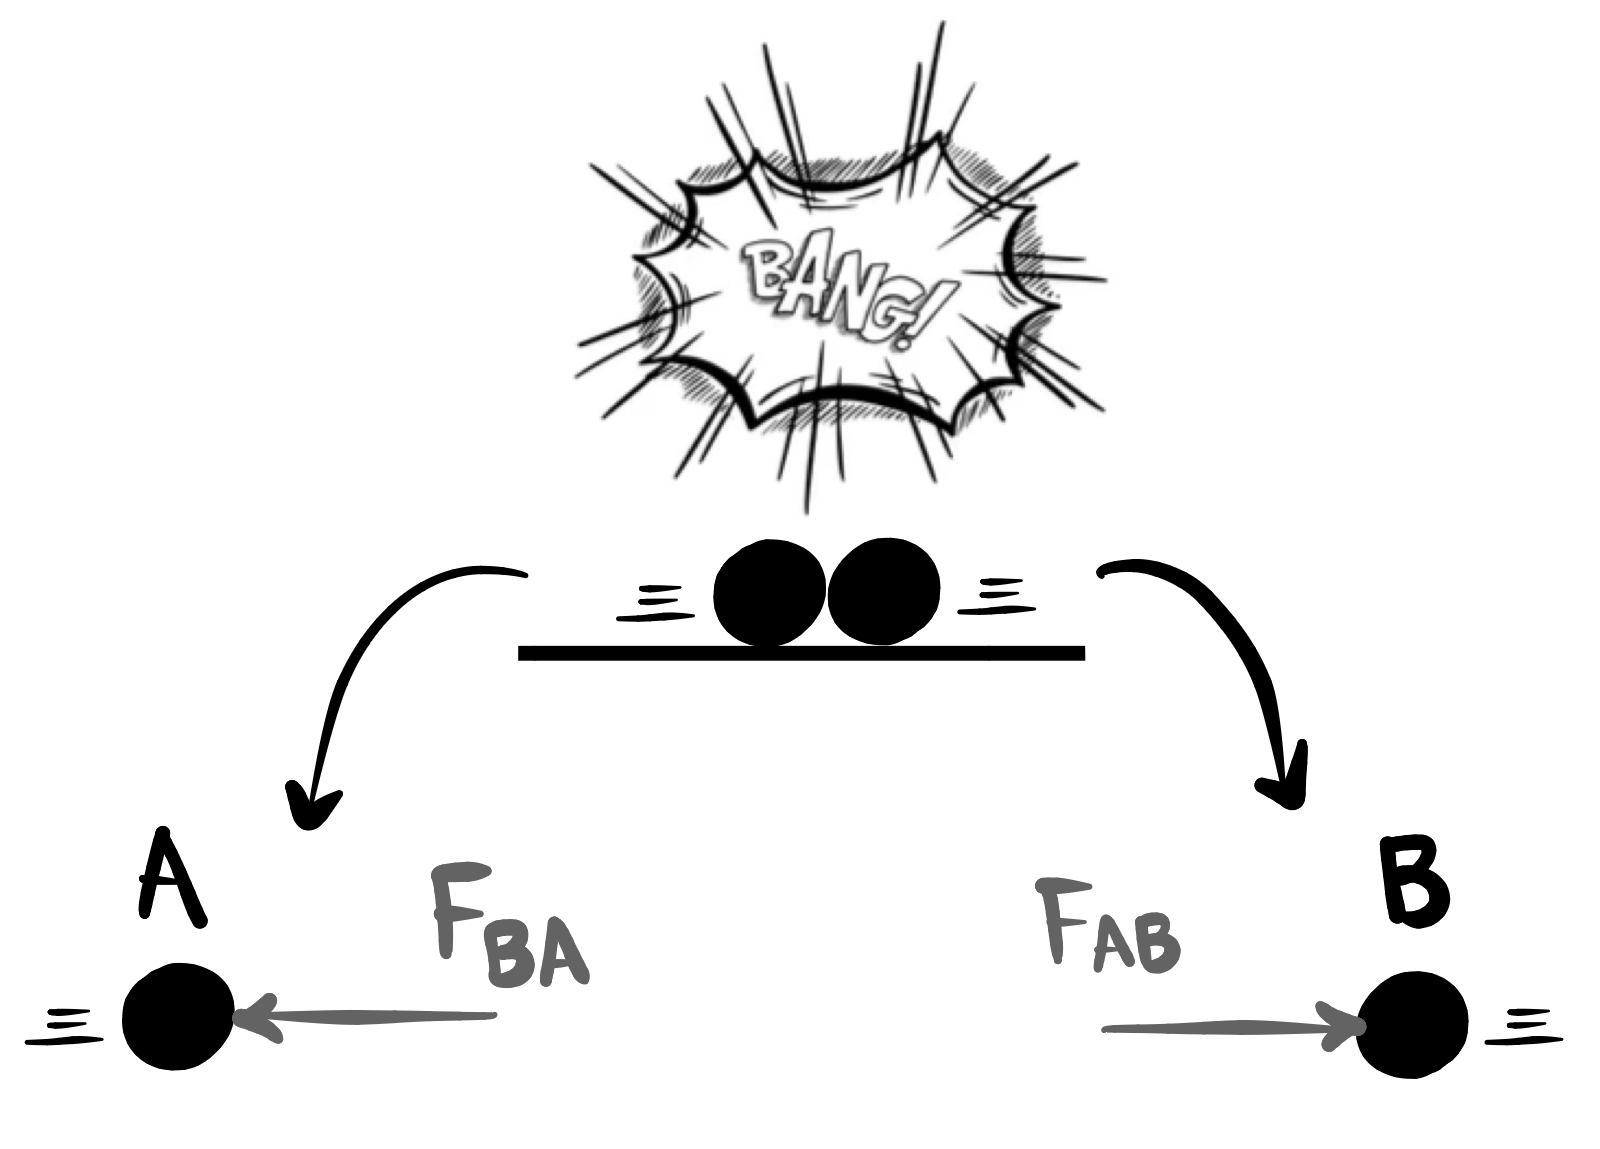
\includegraphics[width=0.4\linewidth]{imagensdinamicanewton/thirdlawcolision.png}};
  \end{scope}
\end{tikzpicture}
\captionof{figure}{Análise das forças de interação durante a colisão.}
\label{fig_dinamicanewton_thirdlawcolision}
} 
\vspace{0.3cm}




\secgfe{Onde é usada}

Como absolutamente todas as forças vem aos pares -- sem exceção -- a Terceira Lei de Newton acaba por aparecer em diversos contextos distintos e é usada para explicar uma enorme quantidade de fenômenos. 

Considere, por exemplo, a situação de uma simples caminhada: ao dar um passo, você está empurrando o chão para trás. Pela terceira lei de Newton, o chão reage e te empurra para frente, e é isso que possibilita que você ande. Essa força trocada entre os seus pés e o chão é chamada de força de atrito, e é por isso que em superfícies muito lisas -- com pouco atrito -- como em uma pista de gelo é bem difícil caminhar. A força de atrito e suas origens serão estudadas em detalhes em seções futuras.

Se você flexiona as pernas para dar um salto, ocorre algo parecido: você está empurrando o chão para baixo, que reage, empurrando você para cima: é por isso que você consegue saltar. \footnote{Sim, você está empurrando o planeta Terra para baixo ao dar um salto. Ocorre que a massa (inércia) dele é tão grande, mas tão grande, mas tão grande que esse seu empurrão sequer o tira do lugar.} A Figura \ref{fig_dinamicanewton_thirdlawatritoandar} mostra essas duas situações. 


\vspace{0.3cm}
{
\centering
\begin{tikzpicture}
  \begin{scope}[blend mode=multiply]
    \node {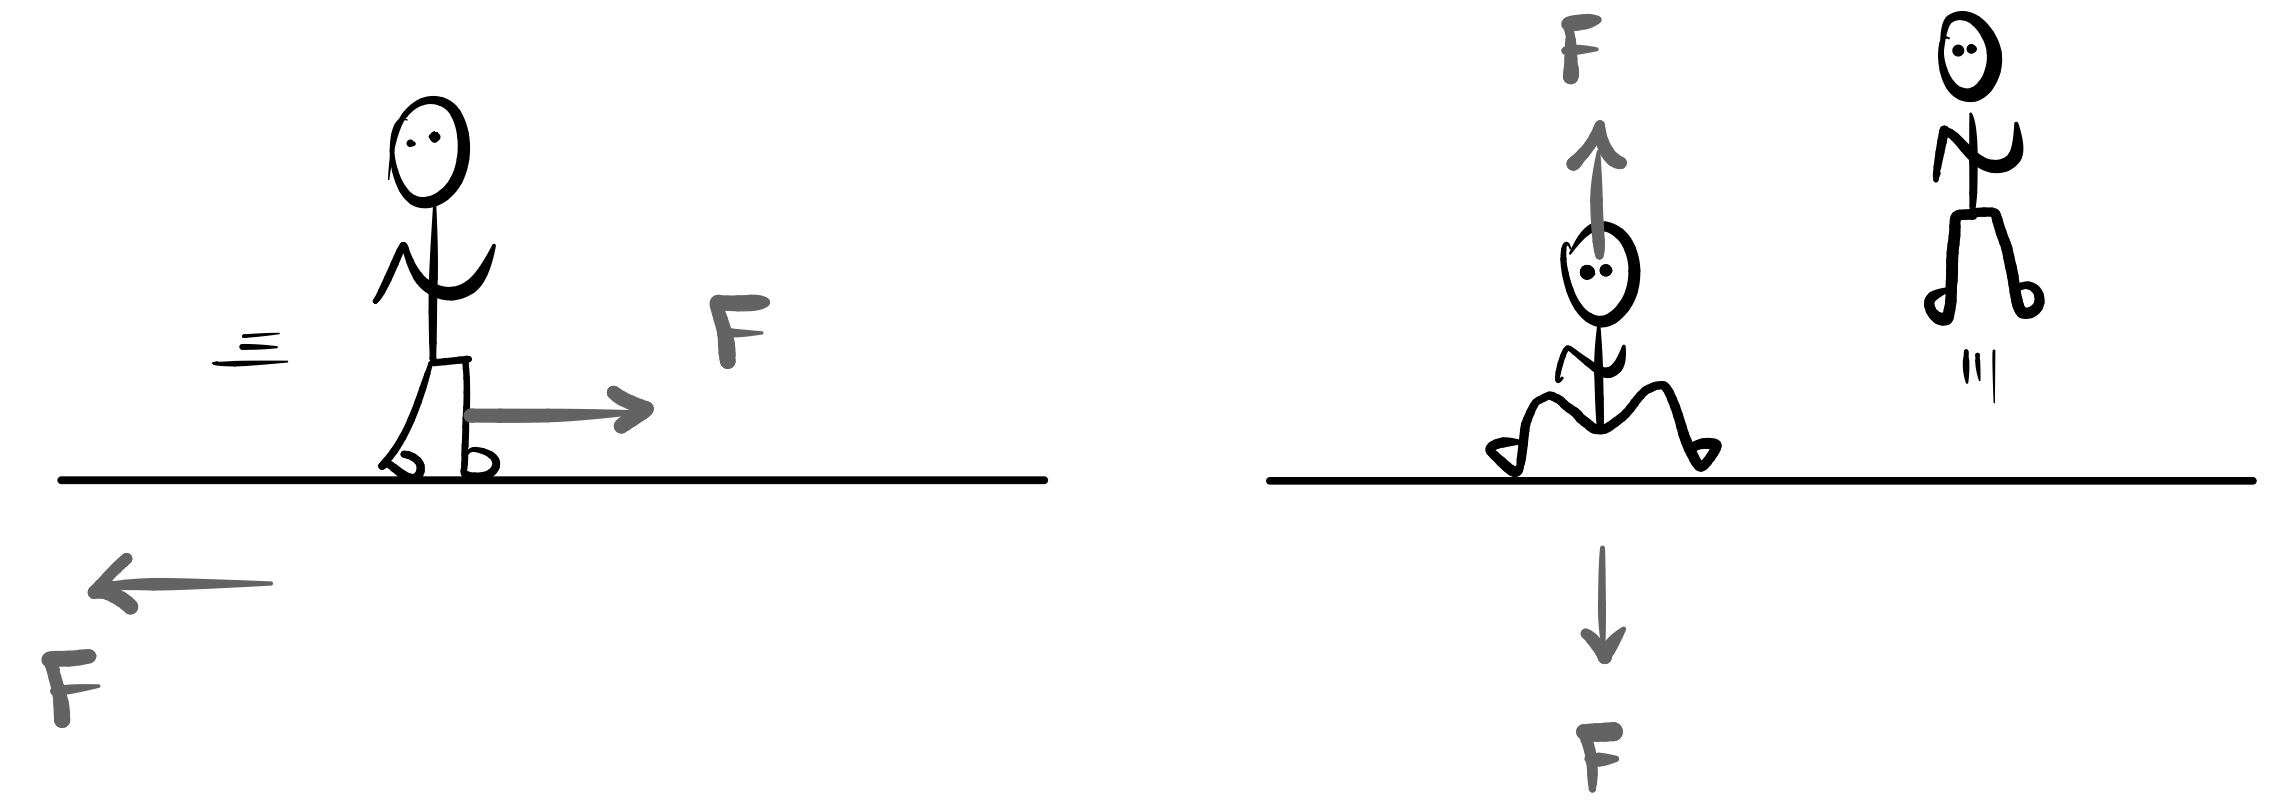
\includegraphics[width=0.55\linewidth]{imagensdinamicanewton/thirdlawexample.png}};
  \end{scope}
\end{tikzpicture}
\captionof{figure}{O par ação-reação das forças trocadas entre o menino e o chão durante uma caminhada e durante um salto, respectivamente.}
\label{fig_dinamicanewton_thirdlawatritoandar}
} 
\vspace{0.3cm}

A Terceira Lei de Newton também explica, por exemplo, como um foguete decola. No interior do foguete, o combustível é queimado, produzindo gases extremamente quentes. Esses gases são expelidos para trás com grande velocidade. Isso significa que o foguete exerce uma força sobre os gases, empurrando-os para trás. Pela Terceira Lei de Newton, os gases devem fazer uma força igual e contrária no foguete, empurrando-o para cima -- essa força propulsora para cima é a que faz o foguete decolar.



Um outro contexto importante que pode ser compreendido sob a luz da Terceira Lei de Newton é o da força que se manifesta em fios, chamada de tração. Observe a Figura \ref{fig_dinamicanewton_thirdlawatraction}, em que um menino puxa uma caixa por uma corda. O menino puxa a corda, na extremidade $1$, com uma força que chamamos de $T_1.$ Pela Terceira Lei, neste mesmo ponto, a corda puxa o menino com uma força igual e contrária. Isso está representado na segunda imagem de tal figura. 

Como o menino puxa a corda, este efeito se propaga e faz com que a corda, que está presa na caixa, puxe a caixa. Chamemos essa força de $T_2.$ Pela Terceira Lei, a caixa deve puxar a corda com uma força igual e contrária.

\vspace{0.3cm}
{
\centering
\begin{tikzpicture}
  \begin{scope}[blend mode=multiply]
    \node {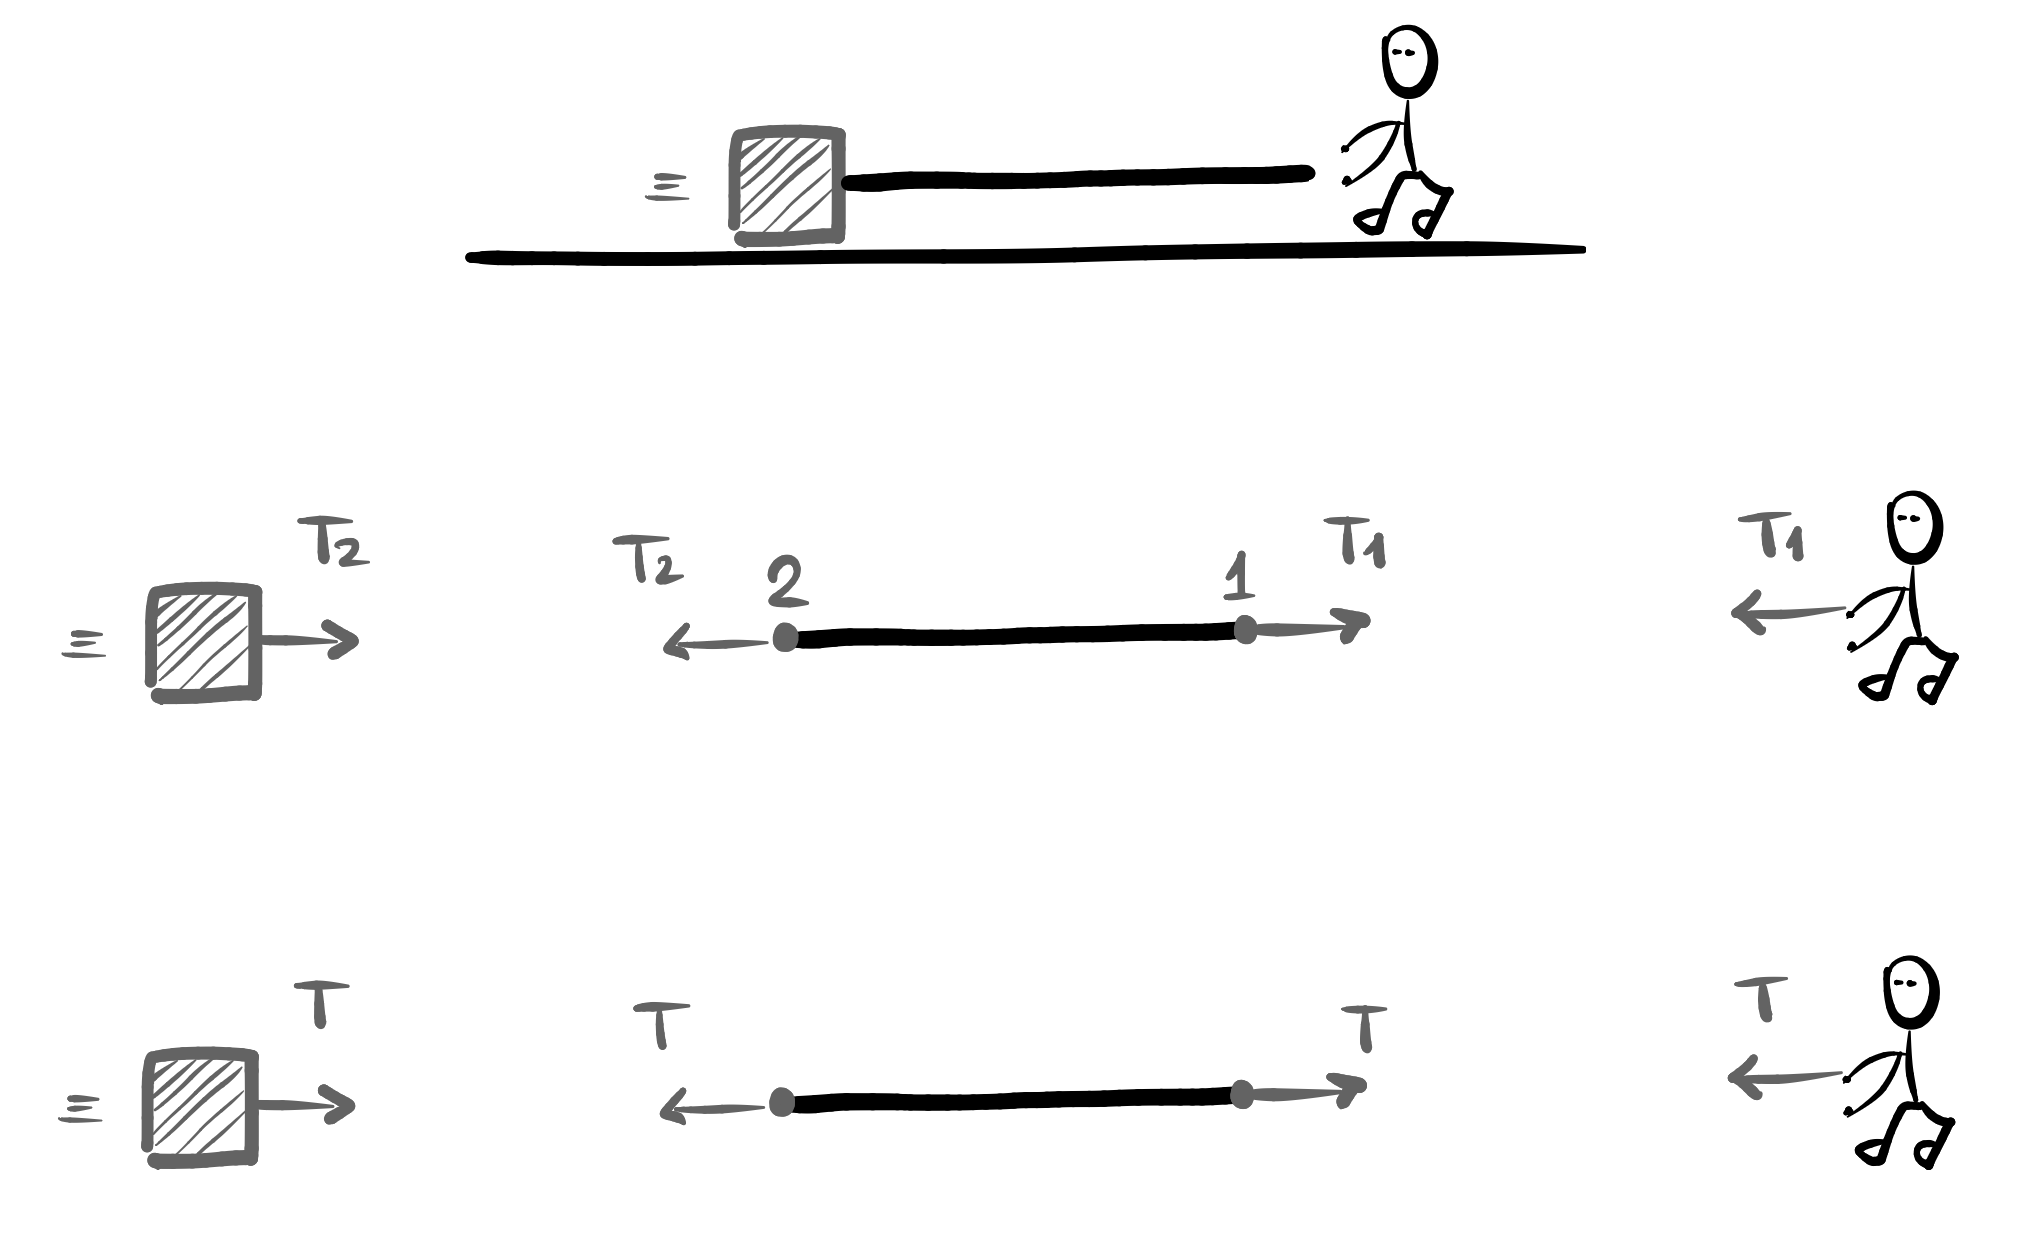
\includegraphics[width=0.8\linewidth]{imagensdinamicanewton/thirdlawtraction.png}};
  \end{scope}
\end{tikzpicture}
\captionof{figure}{A tração em um fio ideal.}
\label{fig_dinamicanewton_thirdlawatraction}
} 
\vspace{0.3cm}

Na quase totalidade dos problemas de Ensino Médio trabalharemos com fios ideais, que são aqueles de massa nula.\footnote{Como o próprio nome diz, é um fio ideal: trata-se de uma idealização, não existe nenhuma corda de massa zero. Isso se trata, na verdade, de uma aproximação: a massa da corda, em geral, será bem menor do que a massa das caixas que serão puxadas, por isso podemos considerar sua massa desprezível. Considere, por exemplo, uma corda de 100g, puxando uma caixa de 50 kg. A massa da corda é de apenas 0.2\% da massa da caixa, de modo que é uma aproximação razoável dizer que sua massa é praticamente zero, se comparada com a da caixa.} Sendo a sua massa nula, a Segunda Lei de Newton nos diz que 

$$ F_R = \cancelto{0}{m} a \implies F_R =0,$$

\noindent portanto, a força resultante em um fio ideal -- estando ele acelerado, parado ou em qualquer estado de movimento -- será sempre nula, ou seja, teremos $T_1=T_2,$ que poderemos chamar apenas de $T,$ para simplificar. Essa conclusão está ilustrada na terceira imagem da Figura \ref{fig_dinamicanewton_thirdlawatraction}: em um fio ideal a força feita em uma extremidade é propagada na íntegra ao longo do fio até a outra extremidade. Assim, no fio ideal, as forças nas suas extremidades -- as trações -- sempre terão o mesmo módulo.











A Terceira Lei de Newton também nos permite compreender uma força muito importante trocada entre dois corpos em contato: a força normal. Considere, por exemplo, uma caixa sob o chão, na superfície da Terra, como mostra a Figura \ref{fig_dinamicanewton_thirdlawnormal}. A caixa possui uma força peso $P$, que a puxa para baixo. Isso faz com que a caixa seja empurrada contra o chão, \textbf{comprimindo o chão}, por meio de uma força que chamamos de força normal $N.$ A caixa, portanto, empurra o chão para baixo, e, pela Terceira Lei, o chão reage e empurra a caixa para cima com uma força de mesmo módulo, direção, porém sentido contrário. \textbf{A força normal, portanto, é uma força de compressão entre duas superfícies em contato, e é sempre perpendicular a tal superfície de contato.}

\vspace{0.3cm}
{
\centering
\begin{tikzpicture}
  \begin{scope}[blend mode=multiply]
    \node {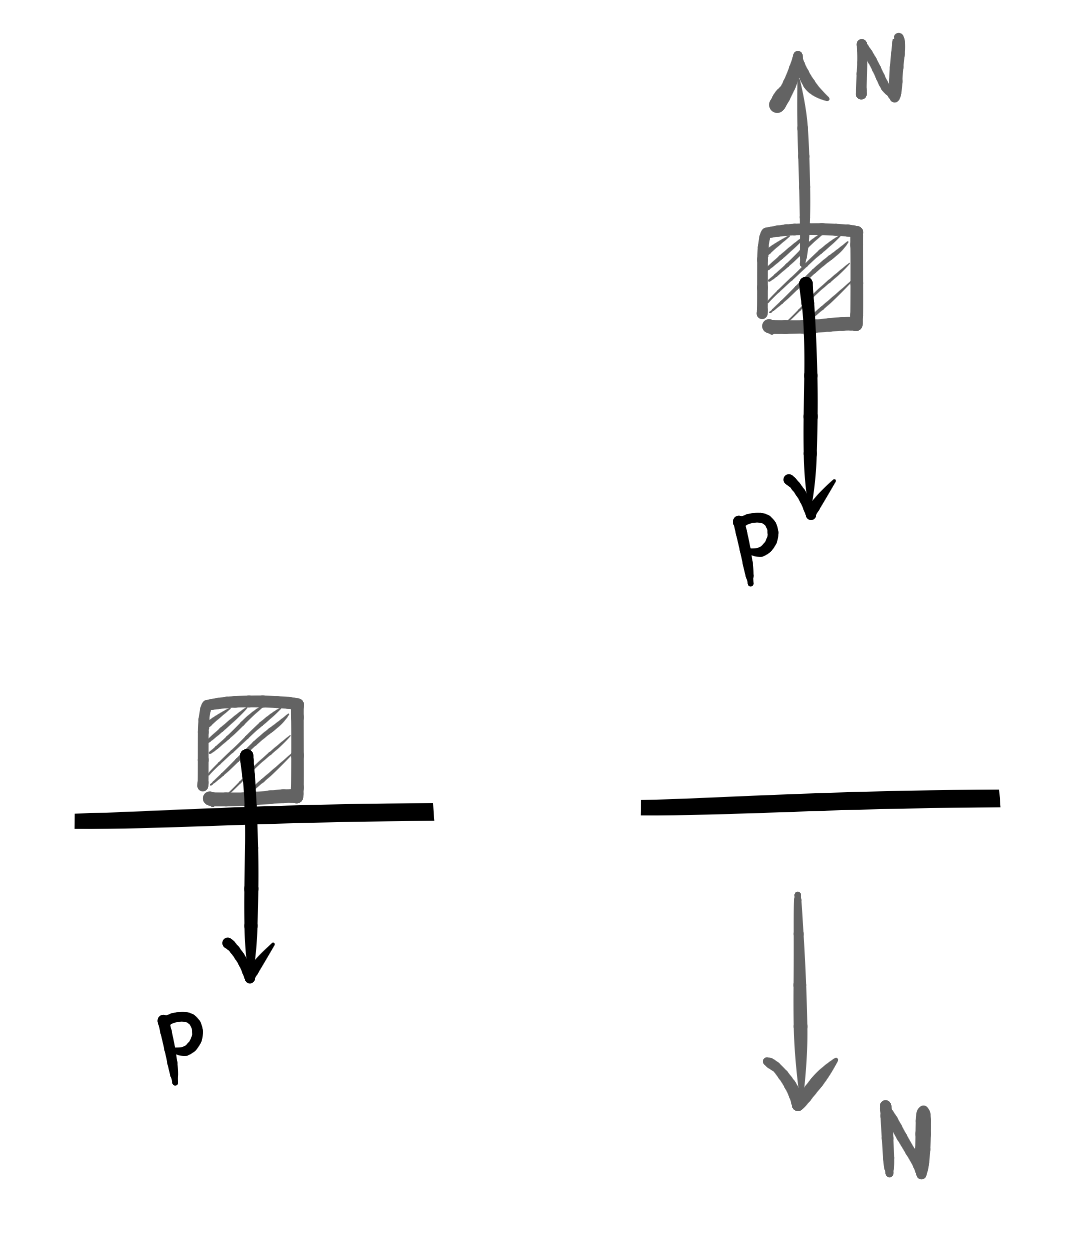
\includegraphics[width=0.3\linewidth]{imagensdinamicanewton/thirdlawnormal.png}};
  \end{scope}
\end{tikzpicture}
\captionof{figure}{A força normal é uma força de contato sempre perpendicular à superfície de contato entre os corpos.}
\label{fig_dinamicanewton_thirdlawnormal}
} 
\vspace{0.3cm}


Note algumas coisas neste contexto:

\begin{enumerate}
    \item [(i)] A força normal é uma força de contato, e recebe esse nome justamente pelo fato de que, em física, normal é sinônimo de perpendicular: a força normal é uma força de contato trocada entre dois corpos que estejam em contato, e tal força é sempre perpendicular à superfície de contato entre os corpos. A Figura \ref{fig_dinamicanewton_normalsempreperpendicular} ilustra algumas outras situações, destacando a força normal de contato entre o corpo e a superfície -- sendo tal força sempre perpendicular (normal) à superfície do corpo apoiado.  



\vspace{0.3cm}
{
\centering
\begin{tikzpicture}
  \begin{scope}[blend mode=multiply]
    \node {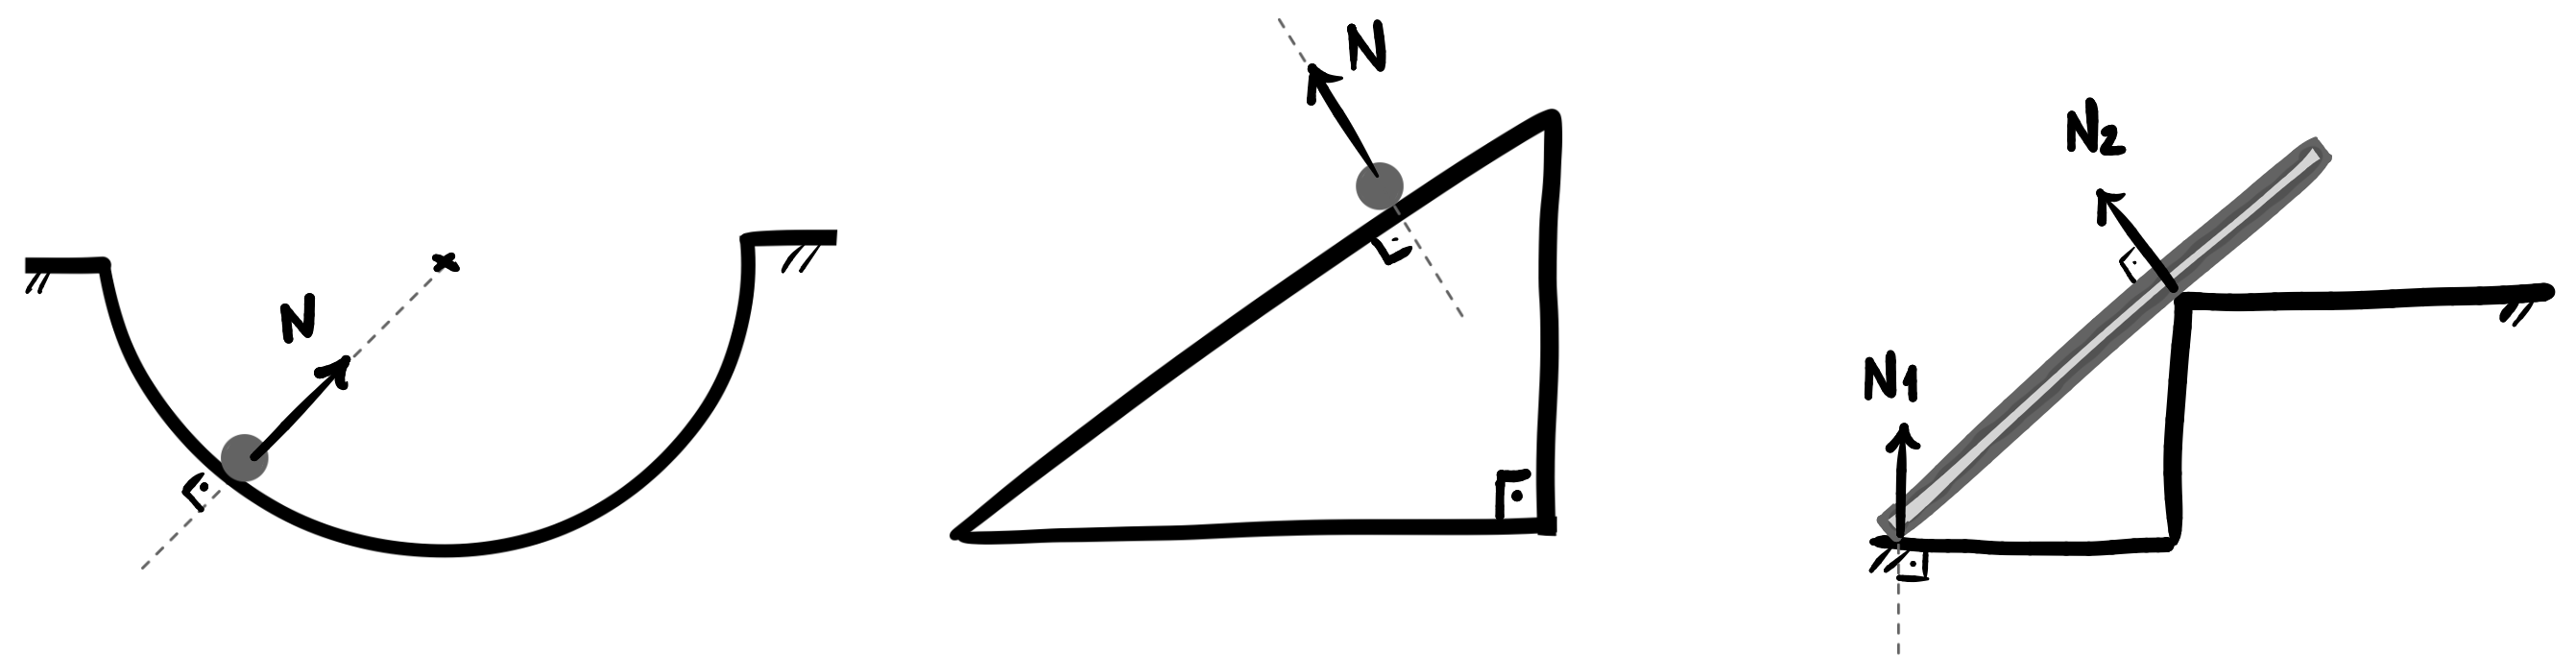
\includegraphics[width=0.95\linewidth]{imagensdinamicanewton/normalsempreperpendicular.png}};
  \end{scope}
\end{tikzpicture}
\captionof{figure}{A força normal é sempre perpendicular à superfície de contato entre os corpos.}
\label{fig_dinamicanewton_normalsempreperpendicular}
} 
\vspace{0.3cm}

Note que, na situação da última imagem da figura, a barra está apoiada em dois pontos -- no solo, horizontal, e na quina da parede vertical com a parede horizontal --, de modo que, tendo dois pontos de contato, existem duas forças normais distintas, representadas por $N_1$ e $N_2$. Note também, ainda nessa situação, que na quinta ficaria difícil de definir a direção perpendicular à superfície de apoio: neste caso, a normal $N_2$ é perpendicular à superfície da barra que está em contato com a quina. 
    
    
    \item [(ii)] Se a caixa estiver em repouso, teremos que $F_R=0,$ de modo que a força para cima deve anular a força para baixo, isto é, $N=P.$

    \item [(iii)] A normal e o peso \textbf{não constituem uma par ação-reação}. Elas, como visto, atuam no mesmo corpo: na caixa. Elas possuem, inclusive, naturezas distintas: a normal é uma força de contato enquanto o peso é uma força de interação gravitacional. O par ação-reação aqui é o par de forças normais trocadas entre o chão e a caixa: a reação da normal na caixa (força que o chão faz na caixa) é a normal no chão (força que a caixa faz no chão). Isso está destacado na segunda imagem da Figura \ref{fig_dinamicanewton_thirdlawnormal}.

    Um leitor mais auspicioso poderia perguntar: \textit{mas qual é a reação do peso na caixa?} Essa pergunta será respondida na subseção seguinte, mas já levanto a bola para o leitor chutá-la: se o peso é a força que a Terra (corpo A) faz na caixa (corpo B), a reação deve ser uma força de mesma natureza feita pelo corpo B no corpo A...conseguiu perceber de qual força se trata?

    
\end{enumerate}







\secgfe{Erros comuns}

A situação da Figura \ref{fig_dinamicanewton_thirdlawnormal} certamente já deve ter levado o leitor a cometer um dos erros mais comuns: não conseguir identificar com clareza quais são os pares ação-reação.

Note, naquele contexto, que a força peso é uma interação gravitacional entre a caixa (corpo $A$) e a Terra (corpo $B).$ Já a força normal é uma interação de contato entre a caixa (corpo $A)$ e o chão (corpo $C).$ Logo, veja que há três corpos em questão interagindo, de modo que, sendo as forças sempre em pares, precisamos analisar as interações dois corpos por vez. O erro muitas vezes cometido é sequer perceber quais são os corpos envolvidos nas interações -- e a representação da própria Figura \ref{fig_dinamicanewton_thirdlawnormal} já induz a este erro, por mostrar apenas dois dos três corpos que estão interagindo com as forças representadas na figura.

O mais correto, portanto, seria colocarmos todos os corpos no nosso esboço, como mostra a Figura \ref{fig_dinamicanewton_thirdlawclassictable}, em que consideramos a caixa apoiada em cima de uma mesa ao invés do chão, apenas para facilitar a representação. 

Perceba, pela primeira imagem, que ao representarmos as forças $P$ e $N$ na caixa, é fácil sermos induzidos ao erro, haja vista que cada uma dessas forças é exercida por um corpo diferente: o peso $P$ é exercido pela Terra, enquanto a força normal $N$ é exercida pela mesa. Assim, é bastante instrutivo separar os corpos dois a dois para analisar cada interação individualmente -- o que é feito nas próximas imagens dessa figura.

\vspace{0.3cm}
{
\centering
\begin{tikzpicture}
  \begin{scope}[blend mode=multiply]
    \node {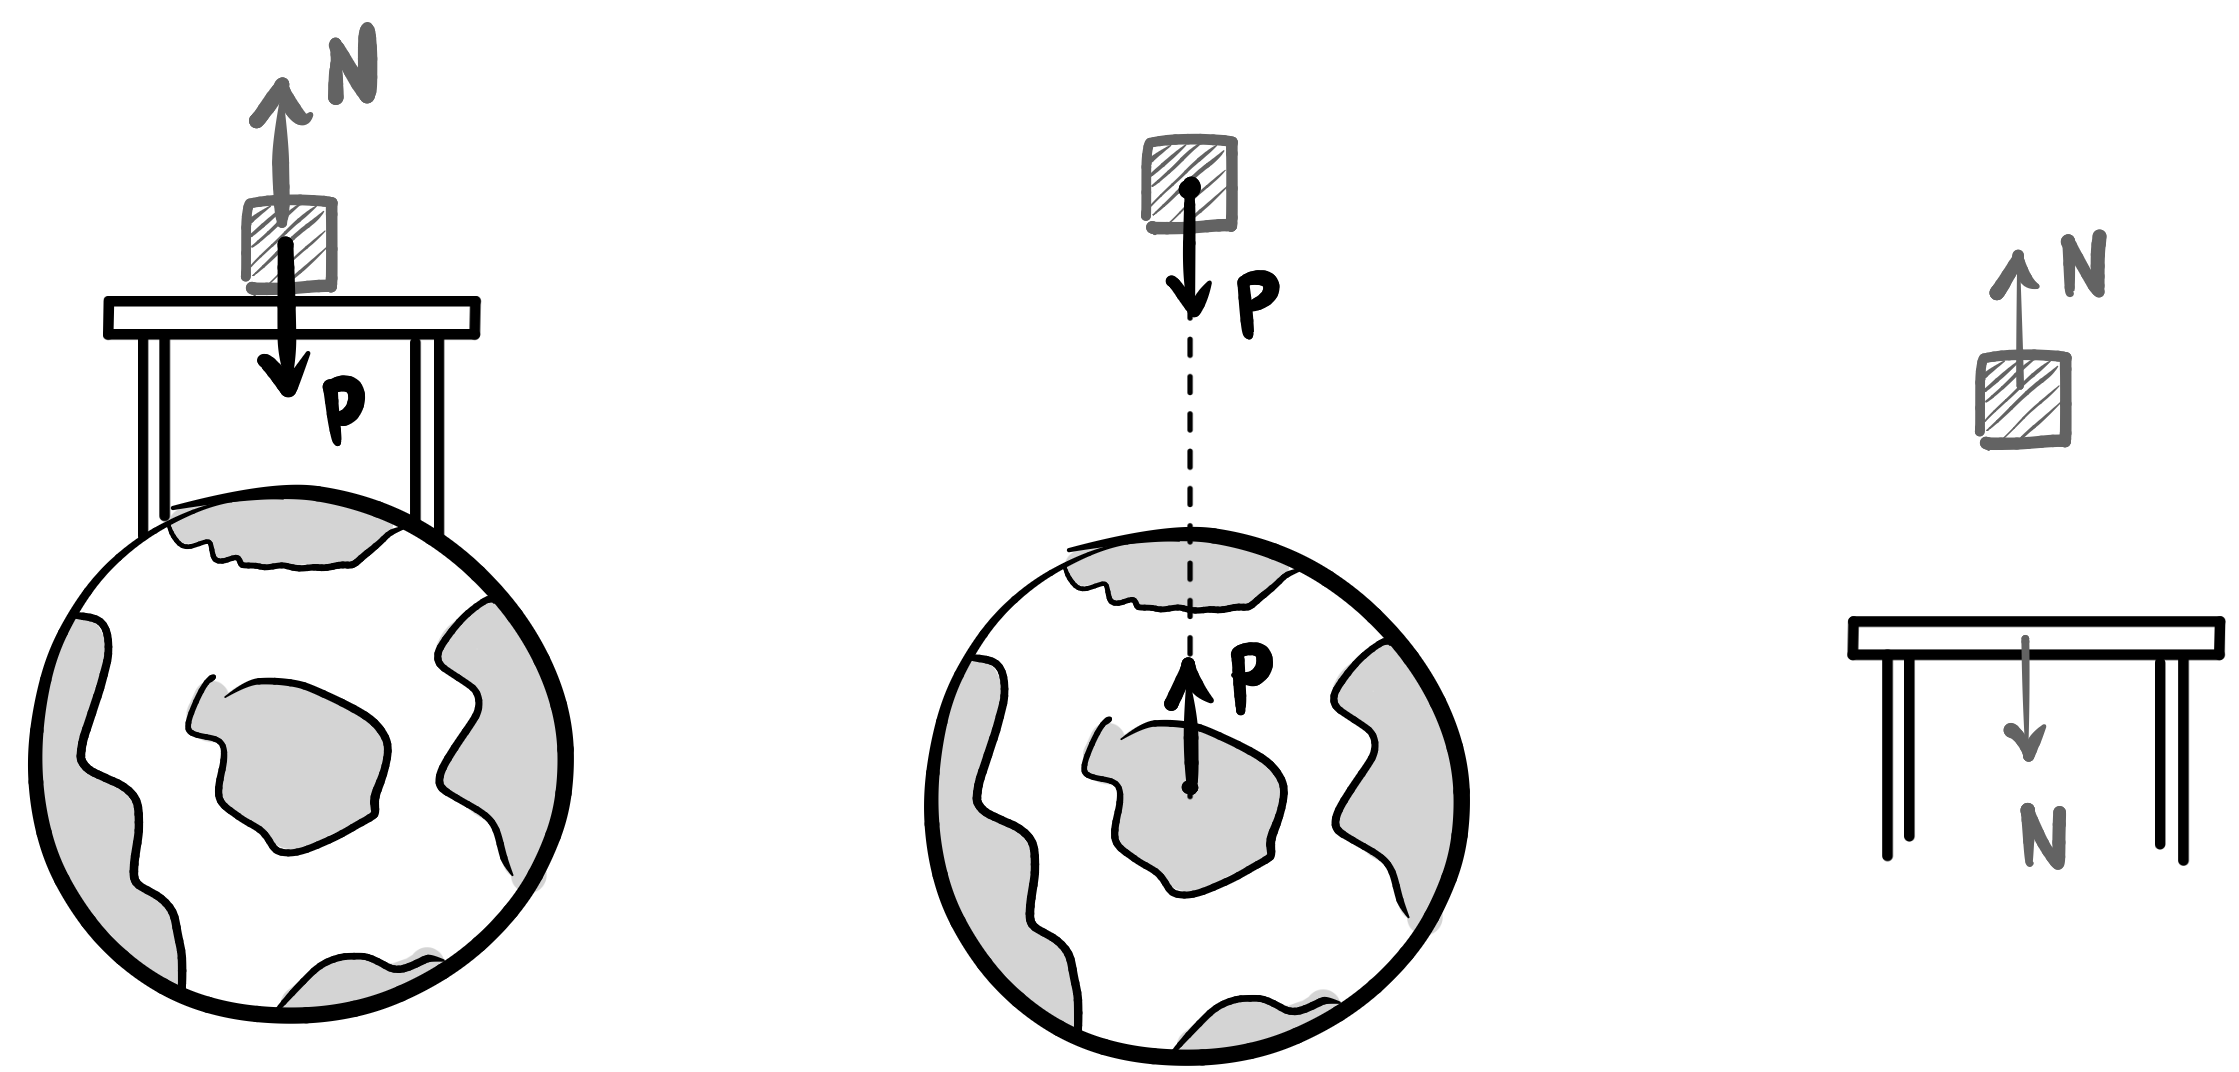
\includegraphics[width=0.6\linewidth]{imagensdinamicanewton/thirdlawclassictable.png}};
  \end{scope}
\end{tikzpicture}
\captionof{figure}{A Terceira Lei de Newton diz que as forças sempre vêm aos pares. Assim, é instrutivo sempre separar os corpos em pares para avaliar a respectiva intereção trocada entre eles.}
\label{fig_dinamicanewton_thirdlawclassictable}
} 
\vspace{0.3cm}


A primeira interação é entre a caixa e a Terra: se a Terra faz uma força $P$, gravitacional, na caixa, então a reação será a caixa fazendo uma força $P$, também gravitacional, de mesmo módulo, direção, porém sentido contrário, na Terra. Portanto, a reação do peso na caixa está no centro do planeta Terra, e é também uma força de natureza gravitacional.\footnote{Como a Terra tem uma massa (inércia) gigante, tal força é irrelevante e não altera o estado de movimento dela.}

Separando agora os outros dois corpos cuja interação nos interessa, temos a caixa e a mesa, na última imagem da Figura \ref{fig_dinamicanewton_thirdlawclassictable}. Por ter um peso que a puxa para baixo, a caixa empurra a mesa para baixo com uma força normal de contato $N.$ Desse modo, a mesa reage e faz uma força normal $N$ na caixa: essas duas forças são de mesma natureza, direção, módulo, porém sentidos contrários: constituem um par ação-reação.


Este é um ótimo exemplo e nos permite discutir os principais erros cometidos ao aplicar a Terceira Lei de Newton. Vamos recapitular brevemente cada um deles para que fique claro ao leitor:


\begin{enumerate}
    \item Achar que par ação-reação são forças que se cancelam. 
    
    O fato de que a normal e o peso se anulam na caixa, na situação da Figura \ref{fig_dinamicanewton_thirdlawclassictable}, já é razão suficiente para termos certeza de que essas duas forças não constituem um par ação e reação. 

    \item Não se dar conta de que o par ação-reação devem ser forças de mesma natureza. 

    Ainda na situação da Figura \ref{fig_dinamicanewton_thirdlawclassictable}: ao avaliar as forças na caixa, temos certeza de que a normal não é reação do peso porque a força peso é de natureza gravitacional, enquanto a normal é uma força de contato. São forças de naturezas distintas e jamais poderiam constituir um par ação-reação.

    \item Não separar adequadamente as forças nos diferentes corpos.

    Como feito em todas as análises, é extremamente instrutivo separar os corpos e representar, isoladamente, as forças em cada um deles. 
    
    Dado que o par ação-reação representa um par de forças trocadas por \textbf{dois corpos que interagem}, cada uma das forças desse par sempre irá atuar em um desses corpos, de modo que facilita muito desenhá-los separada e isoladamente para representar as forças em cada um deles. Foi o que fizemos na Figura \ref{fig_dinamicanewton_thirdlawclassictable}, analisando isoladamente as interações dos corpos de dois em dois: primeiro a Terra com a caixa, depois a caixa com a mesa.


\end{enumerate}




\secgfe{Observações}

Acredito que a observação mais relevante de todas a ser pontuada aqui -- correndo o risco de ser repetitivo -- é o conselho de sempre desenhar os corpos separados para avaliar a força que atua em cada um deles e não se embolar no par ação-reação. Foi isso que fizemos em todas as nossas análises dos exemplos que trouxemos -- incorpore este raciocínio e use-o.


\vspace{0.3cm}


\begin{exemplo}[Nível I]\label{exemplo_newton_terceiralei01}

Dois blocos, $A$ de massa $m_A = 6\,\text{kg}$ e $B$ de massa $m_B = 4\,\text{kg}$,
estão ligados por um fio ideal e repousam sobre uma superfície horizontal sem atrito.
Uma força horizontal $F = 30\,\text{N}$ é aplicada sobre o bloco $A$, conforme a
figura abaixo. 


\begin{center}
    \begin{tikzpicture}[
    >=Stealth,
    font=\small,
    bloco/.style={draw=black, thick, fill=none,
                  minimum width=1.5cm, minimum height=1.5cm}
  ]

  % ── blocos ──────────────────────────────────────────────────────
  \node[bloco] (A) at (0, 0.75)  {};
  \node[bloco] (B) at (3.2, 0.75) {};

  \node at (A.center) [yshift= 5pt]                  {$A$};
  \node at (A.center) [yshift=-7pt, font=\scriptsize] {$6\,\mathrm{kg}$};

  \node at (B.center) [yshift= 5pt]                  {$B$};
  \node at (B.center) [yshift=-7pt, font=\scriptsize] {$4\,\mathrm{kg}$};

  % ── fio ideal entre os blocos ────────────────────────────────────
  \draw[thick] (A.east) -- (B.west);

  % ── força aplicada em A ──────────────────────────────────────────
  \draw[->, line width=1.2pt]
    (-3, 0.75) -- (A.west)
    node[midway, above=2pt] {$F = 30\,\mathrm{N}$};

  % ── superfície ───────────────────────────────────────────────────
  \draw[thick] (-2.2, 0) -- (5, 0);
  \foreach \x in {-2.0,-1.5,-1.0,-0.5,0.0,0.5,1.0,1.5,2.0,2.5,3.0,3.5,4.0,4.5}
    \draw[thin] (\x, 0) -- (\x-0.3, -0.3);

\end{tikzpicture}
\end{center}






Determine:

\begin{enumerate}
    \item [a)] a aceleração do sistema;
    \item [b)] a tração $T$ no fio que conecta os dois blocos.
\end{enumerate}

\resolucao

\begin{enumerate}

    \item [a)] Como os blocos estão ligados por um fio inextensível, eles se movem
    juntos com a mesma aceleração. Podemos, portanto, tratar o sistema como um único
    corpo de massa total $m_A + m_B = 10\,\text{kg}$. Aplicando a Segunda Lei de
    Newton ao sistema:

    $$F_R = (m_A + m_B)\,a \implies 30 = 10\,a \implies \boxed{a = 3\,\text{m/s}^2.}$$

    \item [b)] Com a aceleração conhecida, isolamos agora apenas o bloco $B$. A única
    força horizontal que atua sobre ele é a tração $T$ do fio — e é exatamente isso
    que buscamos. Pela Segunda Lei de Newton aplicada ao bloco $B$:

    $$T = m_B \cdot a = 4 \cdot 3 = \boxed{12\,\text{N.}}$$

    Note que $T < F$: a força $F = 30\,\text{N}$ precisa acelerar o sistema inteiro
    ($m_A + m_B = 10\,\text{kg}$), enquanto a tração $T$ precisa acelerar apenas o
    bloco $B$ ($4\,\text{kg}$). É natural, portanto, que sejam diferentes.

\end{enumerate}


\end{exemplo}

\vspace{0.3cm}





\begin{exemplo}[Nível II]\label{exemplo_newton_terceiralei02}

Um menino empurra uma caixa de massa $m_A=8$kg, que, por sua vez, empurra uma segunda caixa de massa $m_B=4$kg. 

\vspace{0.3cm}
{
\centering
\begin{tikzpicture}
  \begin{scope}[blend mode=multiply]
    \node {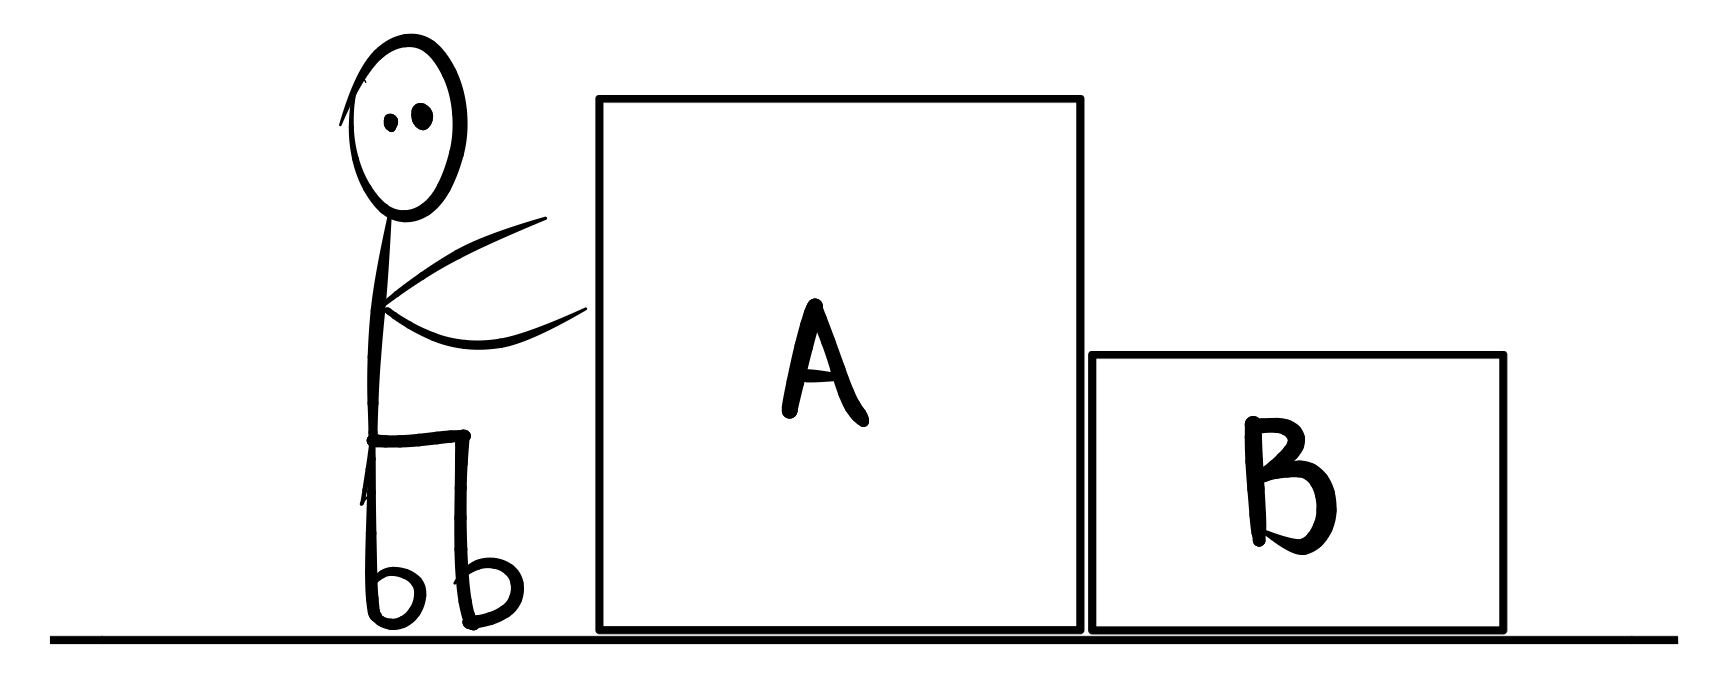
\includegraphics[width=0.4\linewidth]{imagensdinamicanewton/newtonforcasdecontatoexemplo1.png}};
  \end{scope}
\end{tikzpicture}
\captionof{figure}{}
\label{fig_dinamicanewton_newtonforcasdecontatoexemplo1}
} 
\vspace{0.3cm}

Se o menino faz uma força $F=24$N na caixa $A$, calcule:

\begin{enumerate}
    \item [a)] a aceleração do sistema.
    \item [b)] a força de contato entre as caixas.
\end{enumerate}

\resolucao

\begin{enumerate}
    \item [a)] Para computar a aceleração do sistema podemos proceder de duas formas:

    \begin{enumerate}
        \item [(i)] Considerar o sistema das caixas $(A+B)$ como um único corpo.

\vspace{0.3cm}
{
\centering
\begin{tikzpicture}
  \begin{scope}[blend mode=multiply]
    \node {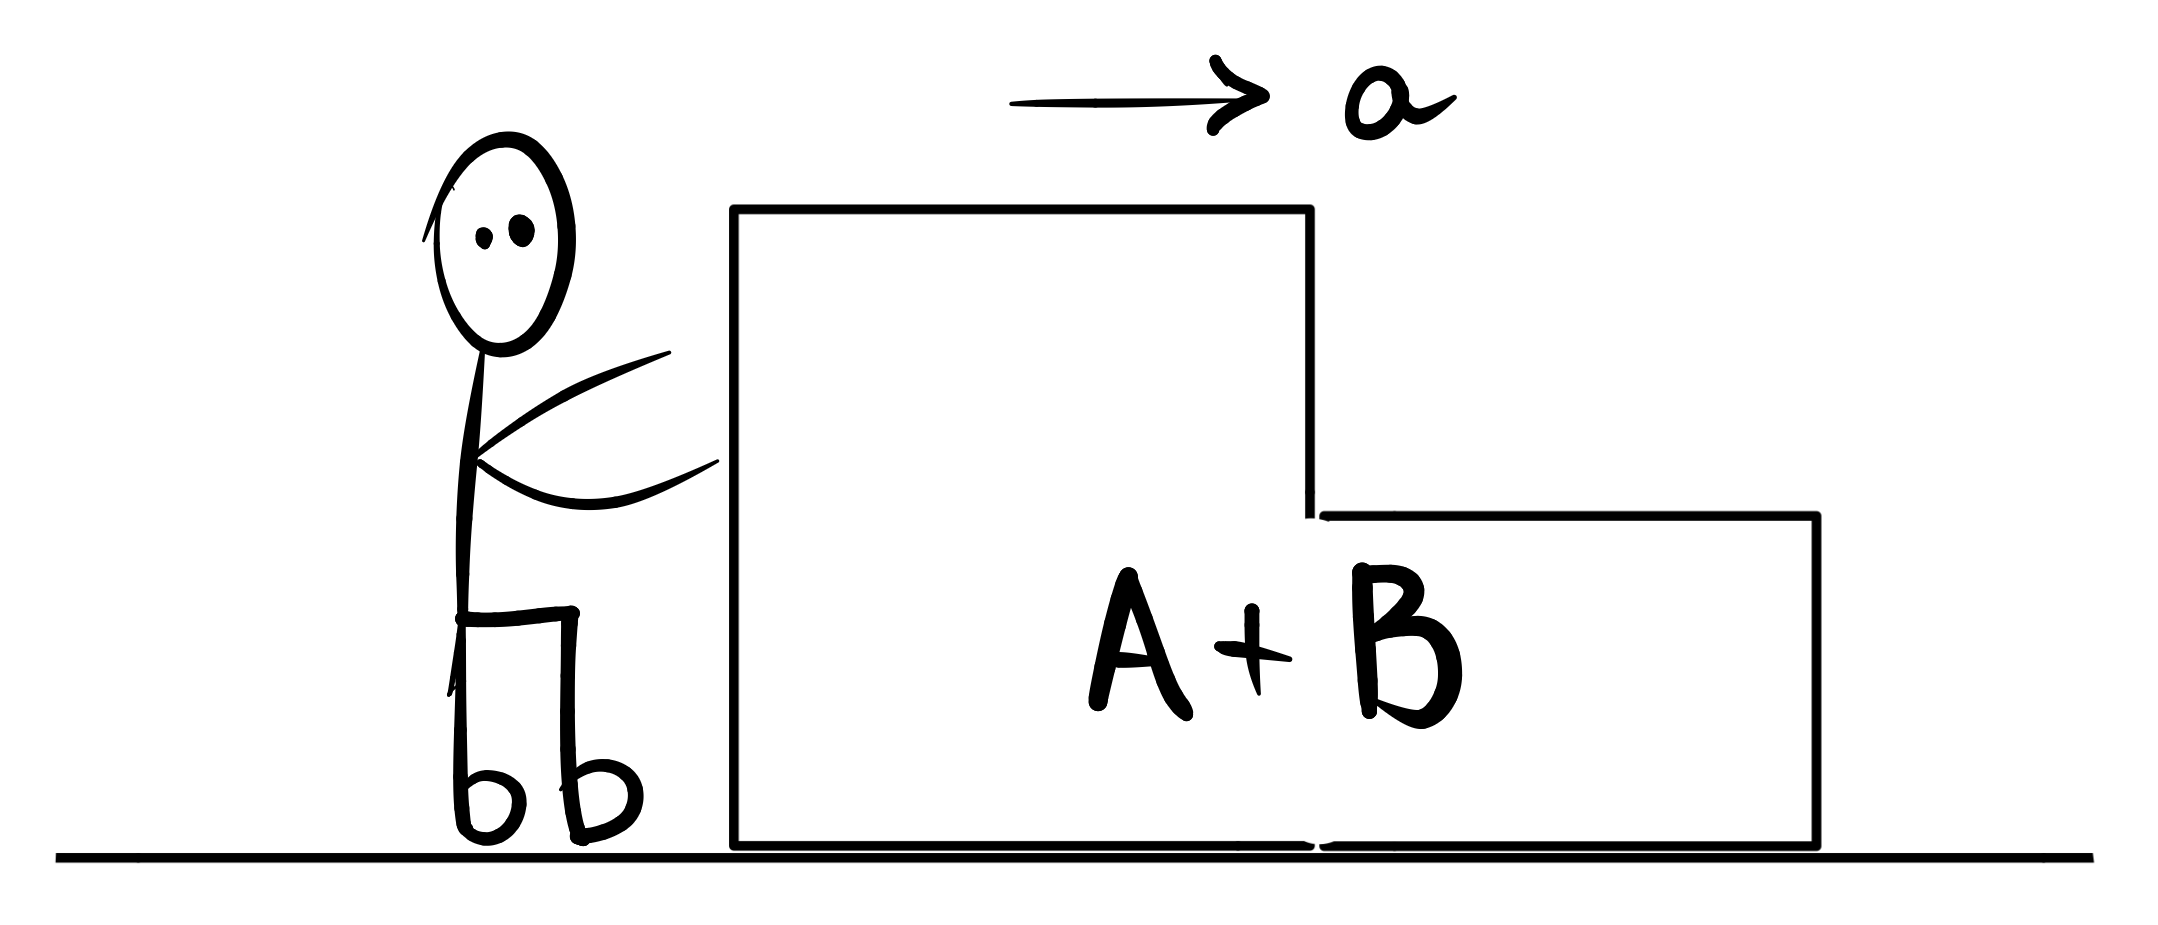
\includegraphics[width=0.4\linewidth]{imagensdinamicanewton/newtonforcasdecontatoexemplo3.png}};
  \end{scope}
\end{tikzpicture}
\captionof{figure}{}
\label{fig_dinamicanewton_newtonforcasdecontatoexemplo3}
} 
\vspace{0.3cm}

        
         Neste caso, o menino, com a força $F=24$N, deve acelerar $8+4=12$kg de massa. Assim, a Segunda Lei de Newton diz que

         $$ F_\text{R} = ma \implies 24 = (8+4)a \implies \boxed{a=2 \text{m/s}^2.}$$

         Note que, se o menino empurra a caixa $A$ de olhos vendados, ele jamais saberia que está tendo que empurrar uma única caixa de 12 kg, ou duas caixas de 6 kg, ou uma caixa de 8 kg e uma de 4 kg, como é o caso. O fato é que sua força $F$ deve ser capaz de acelerar 12 kg de massa, e é por isso que podemos usar este raciocínio de considerar os dois corpos $A$ e $B$ como se fossem um único corpo: porque os dois se moverão juntos, exatamente sob a mesma aceleração $a.$
         

         \item [(ii)] Considerar as caixas $A \text{ e }B$ como corpos separados.

         Neste caso, será preciso desenhar as forças (representaremos apenas as forças horizontais) que atuam individualmente em cada bloco. A Figura \ref{fig_dinamicanewton_newtonforcasdecontatoexemplo2} mostra isso: a caixa $A$ empurra a caixa $B$ com uma força de contato $F_C.$ Pela Terceira Lei de Newton, a caixa $B$ devolve uma força igual e contrária em $A.$

\vspace{0.3cm}
{
\centering
\begin{tikzpicture}
  \begin{scope}[blend mode=multiply]
    \node {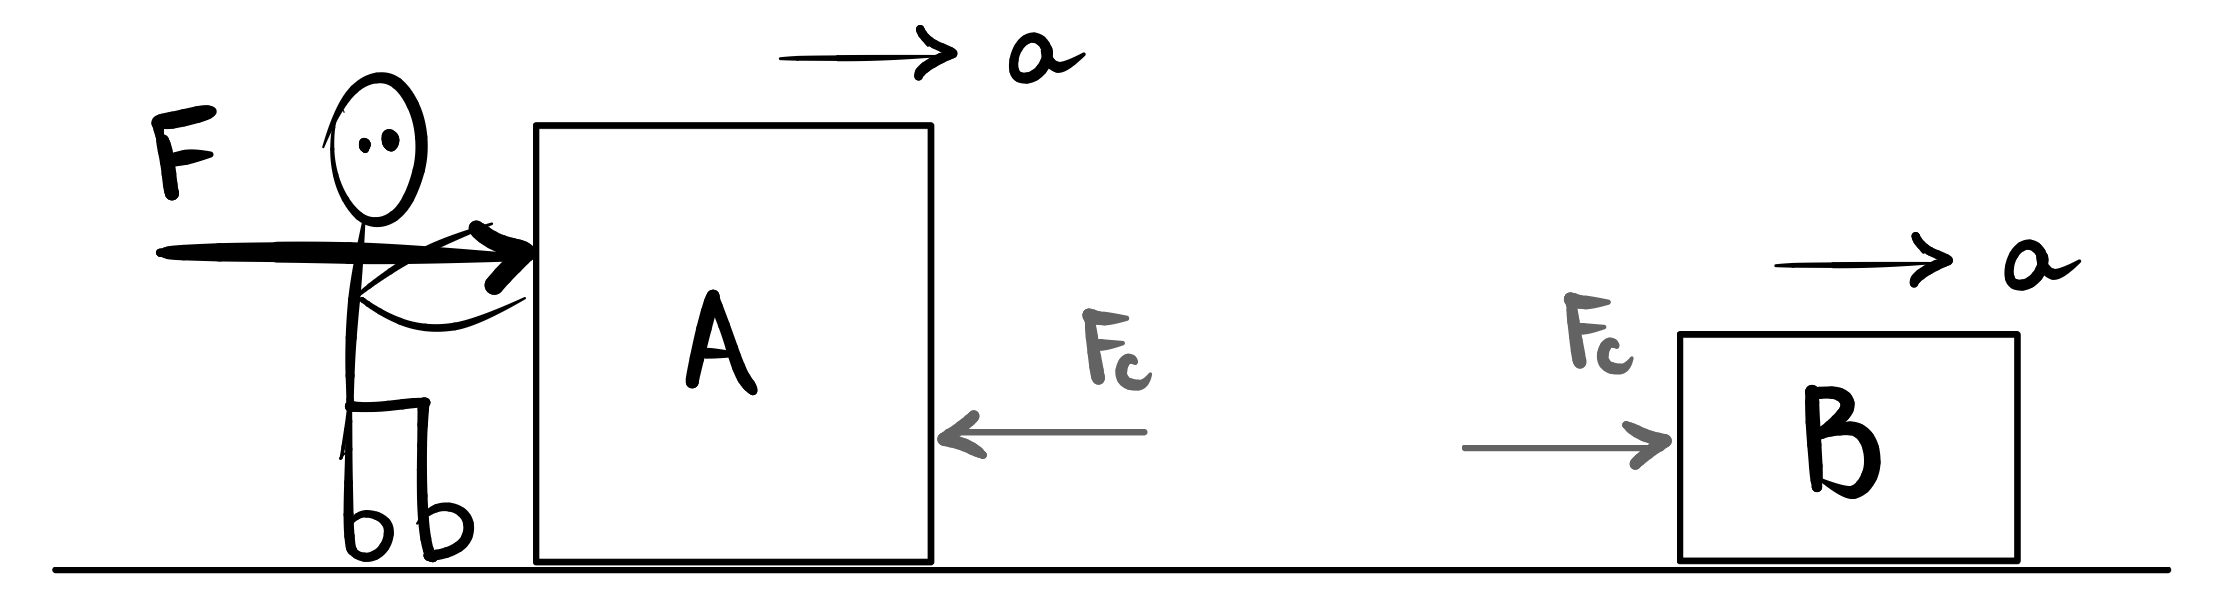
\includegraphics[width=0.65\linewidth]{imagensdinamicanewton/newtonforcasdecontatoexemplo2.png}};
  \end{scope}
\end{tikzpicture}
\captionof{figure}{}
\label{fig_dinamicanewton_newtonforcasdecontatoexemplo2}
} 
\vspace{0.3cm}


         Escrevendo a Segunda Lei de Newton para cada caixa individualmente, teremos, para as forças na horizontal:

         \begin{align}
             F_{\text{R}_A} &= m_A \cdot a_A \implies F - F_C = 8a \nonumber \\
            F_{\text{R}_B} &= m_B \cdot a_B \implies  F_C = 4a, \nonumber
         \end{align}

         \noindent e, somando as duas últimas equações, somos levados a

         $$ \begin{cases} 
           F - \cancel {F_C} = 8a \\
           \cancel {F_C} = 4a
         \end{cases} $$

\noindent ou seja,  $ F = 8a + 4 a = (8+4)a = 12 a.$ Como $F=24$ N, segue que $a= 2$ m/s$^2$, como esperado. Note que esse desenvolvimento prova porque podemos aplicar o raciocínio da solução anterior: ao somar as equações, a força de contato $F_C$ simplifica, restando apenas $F=(8+4)a = (m_A+m_B)a,$ ou seja, podemos olhar para o sistema das caixas como um único corpo -- neste caso, a força de contato desaparecerá, porque será uma força interna a este corpo -- e aplicar a Segunda Lei de Newton $F_R = M_T \cdot a,$ em que $M_T$ seria a massa total do sistema.

Note que isso só pode ser feito porque $a_1=a_2=a,$ isto é, porque os corpos se movem juntos, como se fossem um único corpo.
         
    \end{enumerate}
    
    
    
    \item [b)] Para computar a força de contato $F_C$ entre as caixas, a partir da segunda solução dada no item anterior, basta substituir o valor da aceleração em qualquer uma das equações para os corpos $A$ ou $B$. Fazendo para o corpo $B$, teremos:

    $$ F_C = 4a = 4 \cdot 2 = 8 \text{ N.}$$

    A título de verificação, façamos para a equação de movimento do corpo $A:$

    $$ F - F_C = 8a  \implies 24 - F_C = 8 \cdot 2 \implies F_C = 24 - 16 = 8 \text{ N } \checkmark $$
    
\end{enumerate}



\end{exemplo}



\vspace{0.3cm}


\begin{exemplo}[Nível III]\label{exemplo_newton_terceiralei03}

Tem-se \textit{n} blocos cuja massa cresce de 1 kg a cada bloco, ao se andar da direita para a esquerda, conforme mostra a Figura abaixo.

\vspace{0.3cm}
\begin{center}
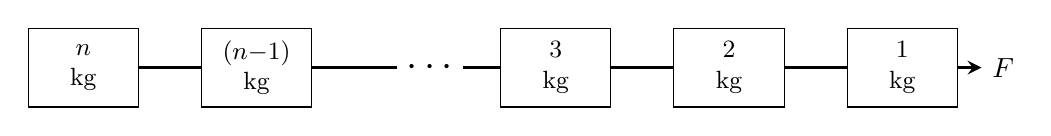
\begin{tikzpicture}[
  block/.style = {draw, minimum width=1.4cm, minimum height=1.0cm,
                  font=\small, align=center},
  wire/.style  = {thick},
  >=stealth
]
  % Blocos da esquerda para a direita
  \node[block] (Bn) at (0,0)     {$n$\\kg};
  \node[block] (Bn1) at (2.2,0)  {$(n{-}1)$\\kg};
  \node        (dots) at (4.4,0) {\Large$\cdots$};
  \node[block] (B3) at (6.0,0)   {$3$\\kg};
  \node[block] (B2) at (8.2,0)   {$2$\\kg};
  \node[block] (B1) at (10.4,0)  {$1$\\kg};

  % Fios
  \draw[wire] (Bn.east)  -- (Bn1.west);
  \draw[wire] (Bn1.east) -- (dots.west);
  \draw[wire] (dots.east) -- (B3.west);
  \draw[wire] (B3.east)  -- (B2.west);
  \draw[wire] (B2.east)  -- (B1.west);

  % Força F
  \draw[->, very thick, black] (B1.east) -- ++(0.3,0)
        node[right, font=\normalsize, black] {$F$};
\end{tikzpicture}
\end{center}
\vspace{0.3cm}
% {
% \centering
% 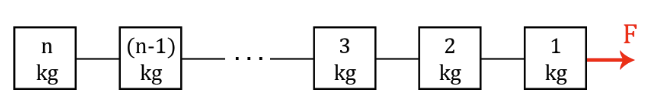
\includegraphics[width=0.6\linewidth]{imagensdinamicanewton/thirdlawexnivel3.png}
% \captionof{figure}{}
% \label{fig_dinamicanewton_thirdlawexnivel3}
% } 
% \vspace{0.3cm}


Os blocos estão conectados entre si por fios ideais e inextensíveis. Ao comunicar ao primeiro bloco -- a contar da direita -- uma força $F$, determine a expressão para a tração no \textit{p-ésimo} fio, em que o primeiro fio é aquele que conecta os blocos de massa 1 kg e 2 kg; o segundo fio é o que conecta os blocos de massa 2 kg e 3 kg, e assim por diante, ou seja, enumera-se os fios a contar da direita.

Discuta as condições de existência de tal expressão.

\resolucao

A chave deste problema é perceber que, uma vez obtida a aceleração do
sistema, a tensão em qualquer fio pode ser determinada isolando um
subsistema conveniente --- exatamente a estratégia que utilizamos no
exemplo anterior. Aqui, a novidade está em generalizar esse
procedimento para $n$ blocos e expressar o resultado em função de $p$.

\medskip
\noindent\textbf{Passo 1 — Aceleração do sistema.}

Tratando os $n$ blocos como um único sistema, todas as tensões internas
se cancelam. A única força horizontal externa é $F$. A massa total é:

\[
  M = 1 + 2 + 3 + \cdots + n = \frac{n(n+1)}{2}.
\]

Pela Segunda Lei:

\[
  a = \frac{F}{M} = \frac{2F}{n(n+1)},
\]

\noindent e todos os blocos do sistema se movem exatamente com essa mesma aceleração. Assim, ao aplicar a Segunda Lei para cada bloco (ou para um conjunto qualquer de blocos) já sabemos qual será a sua aceleração.

\noindent\textbf{Passo 2 — Tensão no $p$-ésimo fio.}

O $p$-ésimo fio (contando da direita) conecta o bloco de $p$\,kg ao
bloco de $(p+1)$\,kg. Para encontrar a tensão $T_p$, isolamos o
subsistema à \emph{esquerda} desse fio: os blocos de massas
$(p+1), (p+2), \ldots, n$\,kg. A única força horizontal sobre esse
subsistema é $T_p$, que o puxa para a direita.

A massa desse subsistema é:

\[
  M_{\text{esq}} = (p+1) + (p+2) + \cdots + n
  = \frac{n(n+1)}{2} - \frac{p(p+1)}{2}
  = \frac{(n-p)(n+p+1)}{2}.
\]

Aplicando a Segunda Lei ao subsistema:

\[
  T_p = M_{\text{esq}}\cdot a
      = \frac{(n-p)(n+p+1)}{2} \cdot \frac{2F}{n(n+1)},
\]

\[
  \boxed{T_p = \frac{(n-p)(n+p+1)}{n(n+1)}\,F.}
\]

\noindent\textbf{Verificação qualitativa.} Para $p = n-1$ (o fio mais
à esquerda, que puxa apenas o bloco de $n$\,kg):

\[
  T_{n-1} = \frac{1 \cdot (2n)}{n(n+1)}\,F = \frac{2F}{n+1}.
\]

Para $p = 1$ (o fio mais à direita, que arrasta todos os demais blocos):

\[
  T_1 = \frac{(n-1)(n+2)}{n(n+1)}\,F.
\]

Em ambos os casos, $T_p < F$, como deve ser: nenhum fio pode exercer
uma força maior do que a força externa que move o sistema inteiro.

\medskip
\noindent\textbf{Condições de existência da expressão.}

A expressão para $T_p$ existe e tem significado físico sob as seguintes
condições:

\begin{itemize}
  \item $n \geq 2$: são necessários pelo menos dois blocos para que
  haja algum fio;
  \item $p \in \{1, 2, \ldots, n-1\}$: $p$ deve ser inteiro positivo
  e não pode superar $n-1$, pois há exatamente $n-1$ fios no sistema;
  \item $F > 0$: a força deve ser não nula para que o sistema acelere e
  os fios fiquem tensionados; se $F = 0$, o sistema está em repouso e todas
  as tensões são nulas.
\end{itemize}

\noindent Para $p = n$, não existe fio --- seria o ``fio à esquerda do
bloco mais à esquerda''. Para $p = 0$, a expressão forneceria $T_0 =
F$, o que corresponderia à tensão imediatamente à direita do bloco de
\SI{1}{kg} --- ou seja, a própria força aplicada. Isso é formalmente
consistente, mas não há fio nessa posição: é apenas a continuidade
algébrica da fórmula além de seu domínio físico.



\end{exemplo}






\begin{secnivel}[Aceleração no Plano Inclinado]{I}{Aceleração no Plano Inclinado}
  
  \eqLdois{dem}{eq_dinamicanewtoniana_gsintheta}{a= g \sin (\theta)}

\end{secnivel}





\secgfe{De onde vem}

A Equação \eqref{eq_dinamicanewtoniana_gsintheta} fornece qual é a aceleração $a$ de um corpo que se move, exclusivamente sob a ação da gravidade, escorregando ao longo de um plano inclinado de $\theta$ em relação à horizontal em uma região em que a gravidade vale $g.$ 

Vamos construir tal equação, passando pausada e calmamente por cada etapa da resolução de um problema qualquer no campo da Dinâmica. Considere a Figura \ref{fig_dinamicanewton_planoinclinado01}. Vamos tentar dividir em etapas o nosso raciocínio:

\begin{enumerate}
    \item [(i)] Começamos desenhando as forças que atuam no corpo que queremos estudar -- no caso, a caixa. A força em questão -- que fará ela escorregar plano abaixo -- é o peso.

\vspace{0.3cm}
{
\centering
\begin{tikzpicture}
  \begin{scope}[blend mode=multiply]
    \node {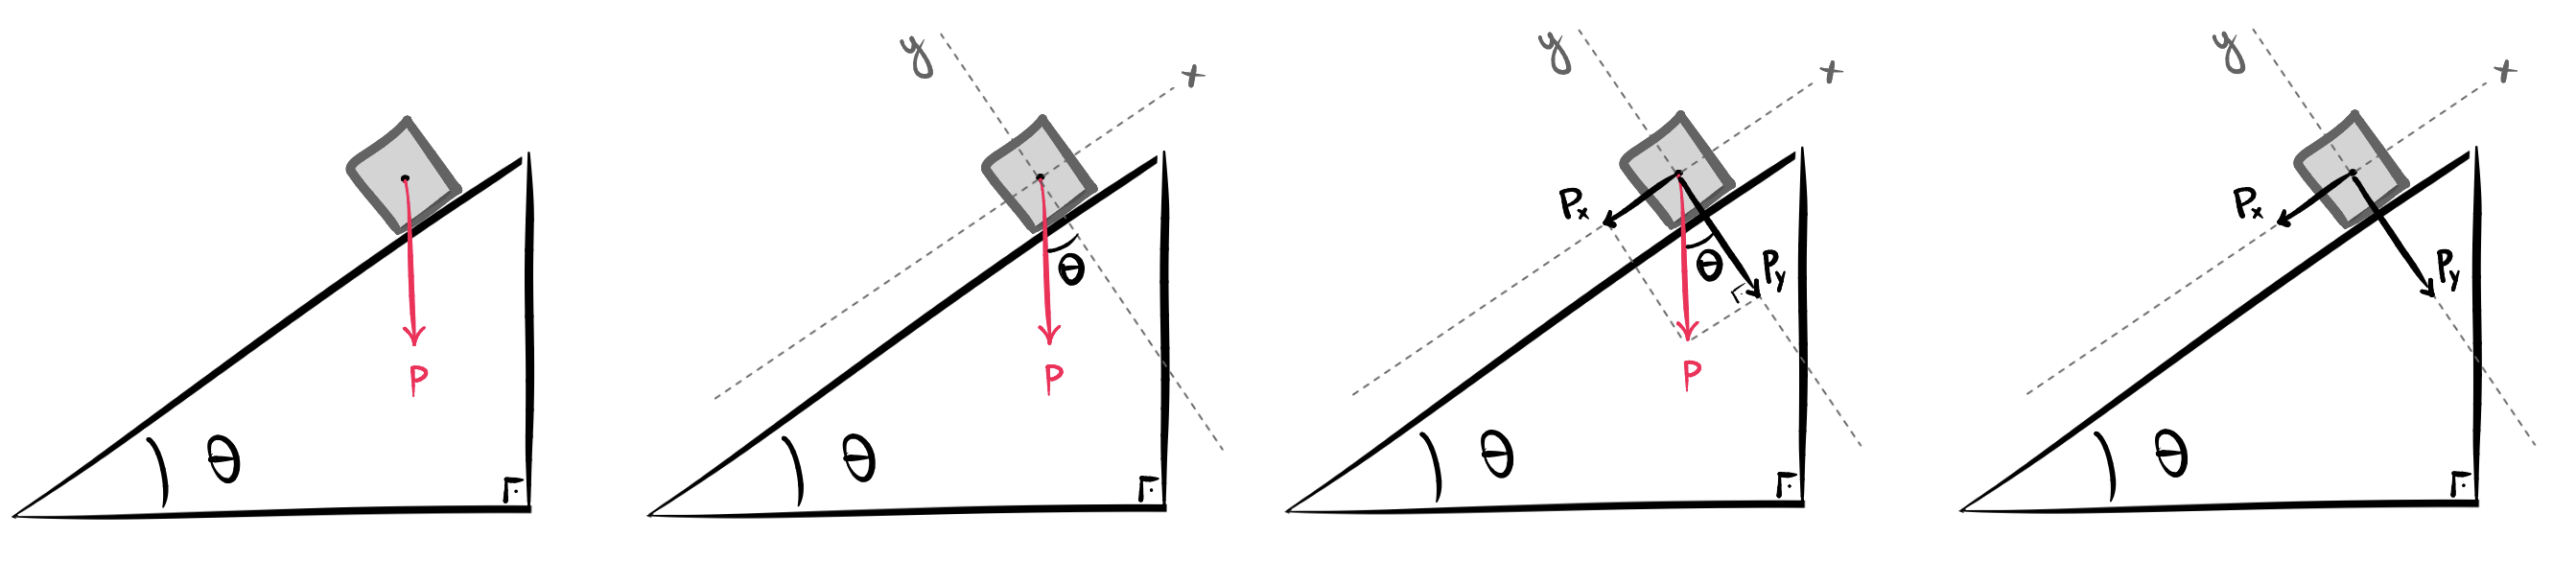
\includegraphics[width=1.0\linewidth]{imagensdinamicanewton/planoinclinado.png}};
  \end{scope}
\end{tikzpicture}
\captionof{figure}{Decomposição de forças no plano inclinado.}
\label{fig_dinamicanewton_planoinclinado01}
} 
\vspace{0.3cm}

\item [(ii)] O segundo passo é definir um sistema de eixos (sempre perpendiculares, como já explicamos ao estudar os vetores) nos quais iremos decompor as eventuais forças. \textbf{Um dos eixos sempre será aquele da direção na qual o movimento se dá, ou, caso prefira, este eixo será sempre paralelo ao vetor velocidade da partícula.} No caso, como ela irá escorregar plano abaixo, tal eixo será paralelo ao plano, representado na segunda imagem pelo eixo $x.$ O outro eixo, sendo perpendicular ao primeiro, será, portanto, perpendicular ao plano, representado pelo eixo $y.$

\item [(iii)] Definido o sistema de eixos, basta fazer a decomposição: isso aparece na terceira imagem da figura, e as componentes podem ser obtidas de forma direta usando as razões trigonométricas no triângulo retângulo dos vetores:

$$ \sin \theta = \dfrac{P_x}{P} \implies \boxed{P_x = P \sin \theta} \quad \text{ e } \quad \cos \theta = \dfrac{P_y}{P} \implies \boxed{P_y = P \cos \theta.} $$

Estamos, neste momento, interessados na resultante das forças na direção $x$: sendo essa a direção do movimento da caixa é nessa direção que aponta a velocidade da partícula, assim, a resultante das forças nessa direção será responsável pela aceleração tangencial:

$$ \sum F_x = ma_x \implies P \sin \theta = ma_x \implies \cancel{m}g \sin \theta = \cancel m a_x \implies \boxed{a_x = g \sin\theta,}$$

\noindent o que fornece a aceleração $a_x$ da caixa ao longo do plano.

\end{enumerate}

O passo-a-passo acima será basicamente a estrutura central de raciocínio para resolver qualquer problema de dinâmica. Algumas dúvidas, contudo, são naturais d surgirem no processo. A primeira delas, provavelmente, é sobre o ângulo $\theta$ do plano inclinado aparecer magicamente no triângulo dos vetores, entre a direção vertical e a direção perpendicular ao plano. 

\vspace{0.3cm}
{
\centering
\begin{tikzpicture}
  \begin{scope}[blend mode=multiply]
    \node {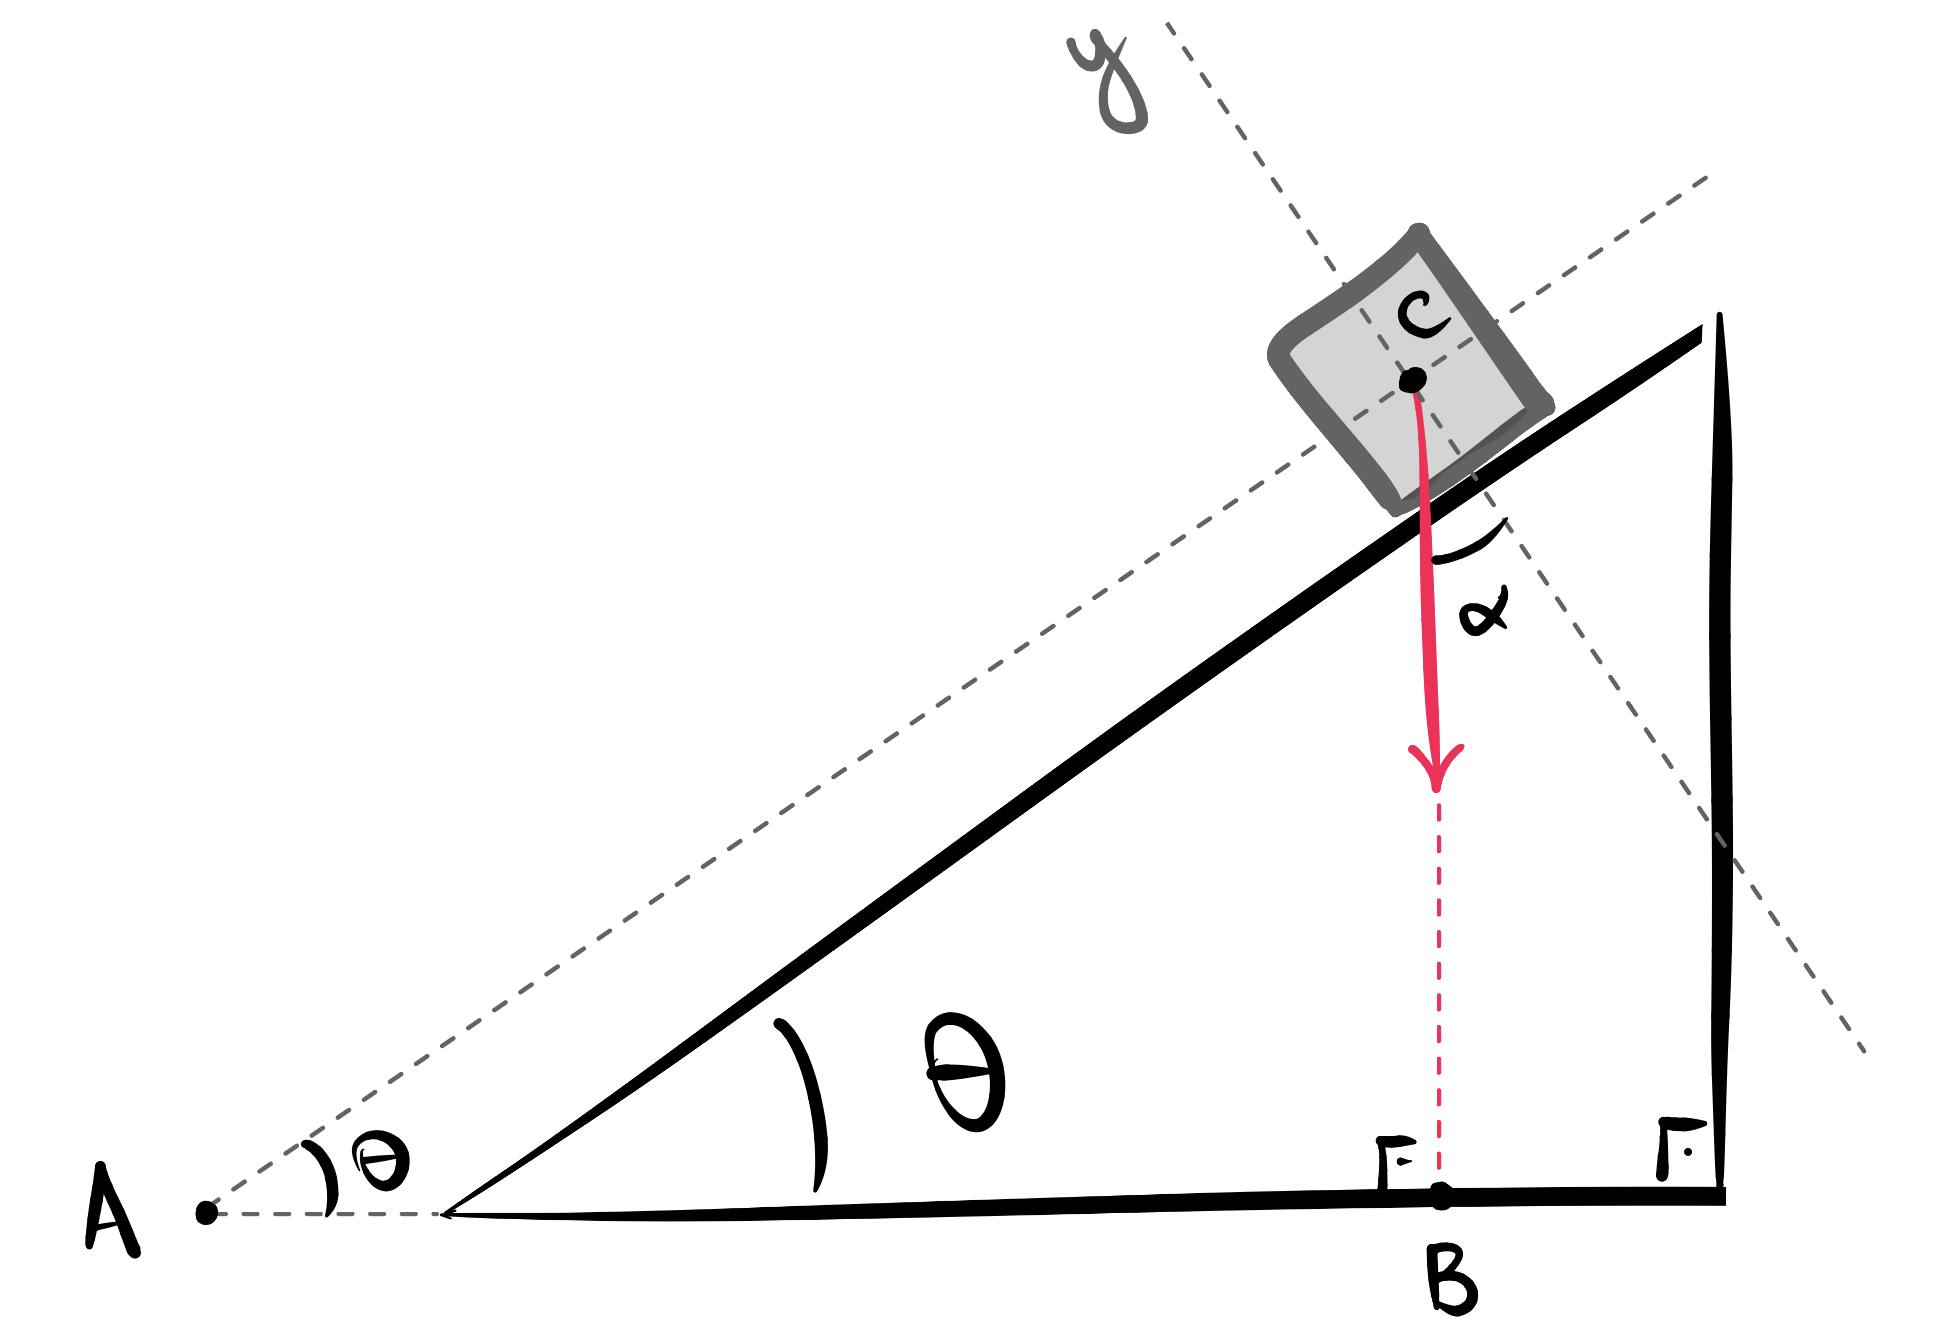
\includegraphics[width=0.35\linewidth]{imagensdinamicanewton/anguloplanoinclinado.png}};
  \end{scope}
\end{tikzpicture}
\captionof{figure}{O ângulo do plano inclinado no diagrama de vetores.}
\label{fig_dinamicanewton_planoinclinado02}
} 
\vspace{0.3cm}

A Figura \ref{fig_dinamicanewton_planoinclinado02} mostra um caminho possível para compreender como podemos encontrar tal ângulo: seja $C$ o ponto de aplicação da força peso, na caixa. Prolongue a direção da força peso até encontrar o solo, no ponto $B.$ Agora prolongue a direção $x,$ paralela ao plano inclinado, até encontrar o chão, no ponto $A.$ O ângulo $B\hat{A}C$ e o ângulo $\theta$ são correspondentes, de modo que suas medidas são iguais: $B\hat{A}C = \theta.$

Note, no triângulo $ABC$, que o ângulo $B\hat{C}A$ é complementar de $\theta$, e o ângulo $\alpha$ destacado é o complementar\footnote{Porque os eixos $x$ e $y$ são perpendiculares.} de $B\hat{C}A$, ou seja:

 $$ \alpha = \dfrac{\pi}{2} - \left( \dfrac{\pi}{2} - \theta \right) = \theta,$$



\noindent de modo que fica provado que o ângulo $\theta$ de inclinação do plano em relação à horizontal aparece entre a direção vertical e a direção perpendicular ao plano.


Uma segunda dúvida que poderia surgir é quanto à componente $P_y = P \cos \theta$ da força peso na direção perpendicular ao plano. Um primeiro comentário importante é o seguinte: as forças na direção perpendicular à direção $x$ são irrelevantes para o cálculo da aceleração na direção $x.$ Movimentos em direções perpendiculares são independentes, esse é um princípio enunciado por Galileu e que é crucial para a análise que fizemos: a aceleração na direção $x$ é determinada única e exclusivamente pela resultante das forças na direção $x$. Desse modo, podemos, como foi feito, isolar o problema e tratar separadamente apenas das componentes de força na direção do plano, uma vez que o que queremos computar é o valor da aceleração na direção do plano.

Dito isso, poderíamos fazer a análise das forças na direção $y$ -- apenas para enriquecer nossa discussão, uma vez que tais forças serão irrelevantes para o cálculo da aceleração na direção $x.$ Neste caso, vale separar os dois corpos em questão: a caixa e o plano inclinado. Por ter uma componente de peso $P_y$ puxando a caixa contra o plano, isso faz com que a caixa exerça uma força normal $N$ sob o plano inclinado, empurrando ele nessa direção. Pela Terceira Lei de Newton, o plano reage e faz uma força igual e contrária na caixa, como está representando na Figura \ref{fig_dinamicanewton_planoinclinado03}. 

\vspace{0.3cm}
{
\centering
\begin{tikzpicture}
  \begin{scope}[blend mode=multiply]
    \node {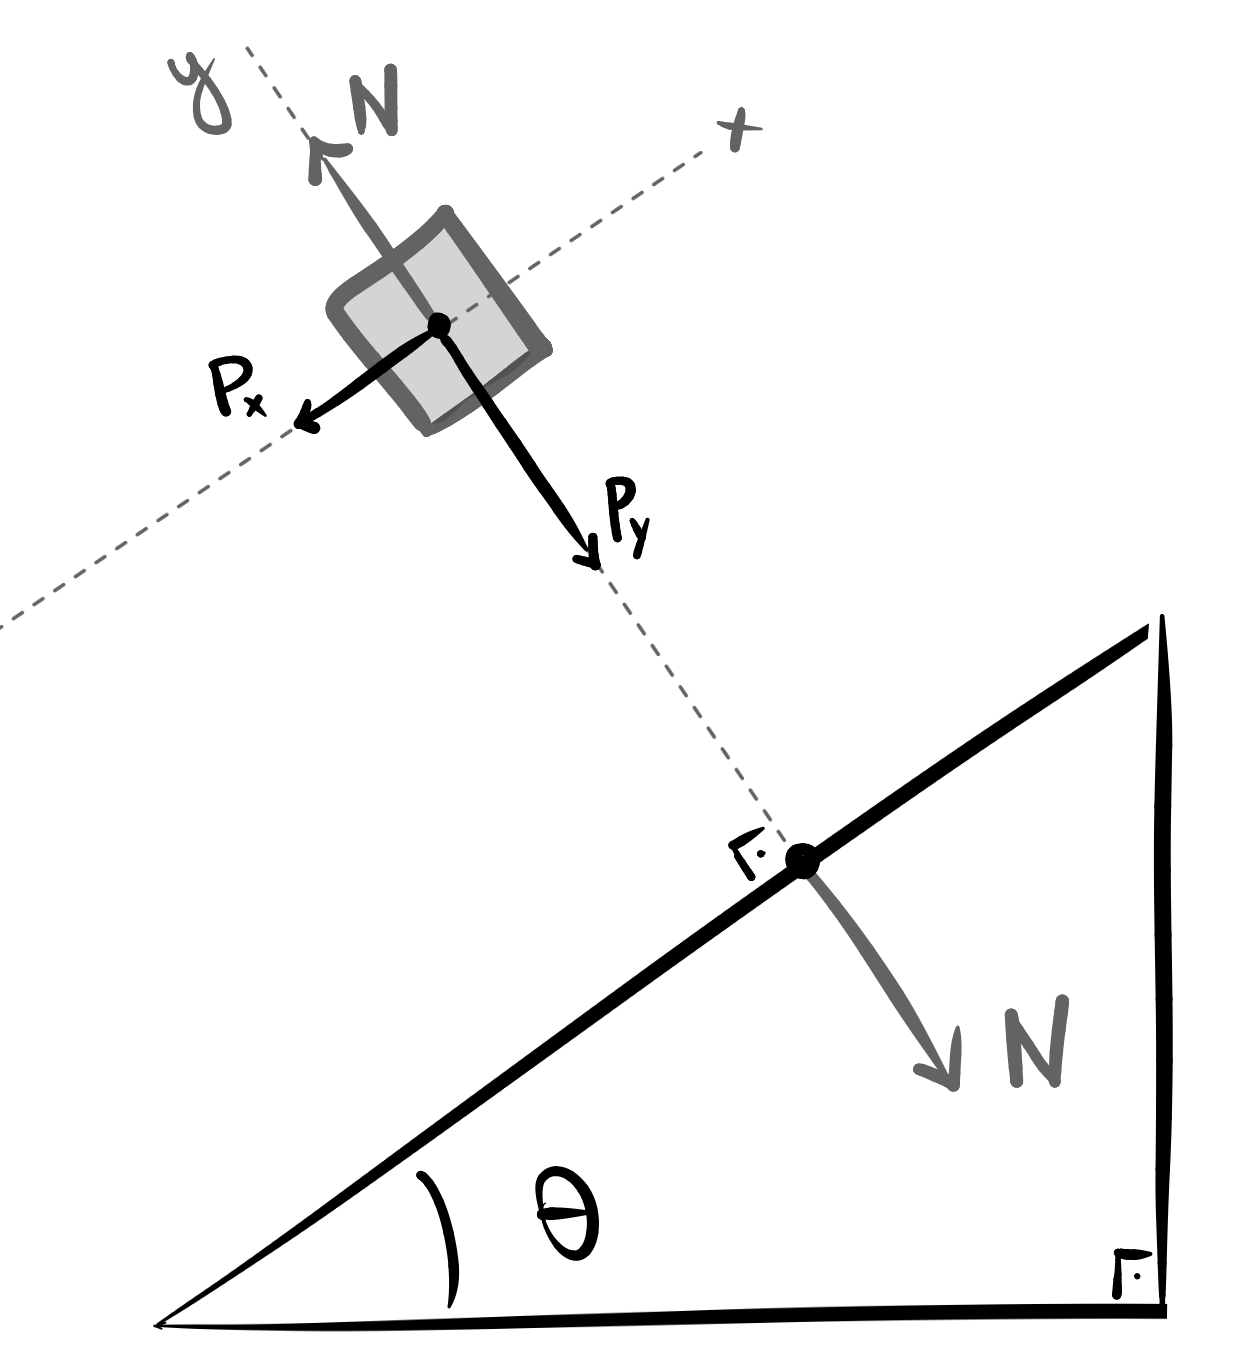
\includegraphics[width=0.3\linewidth]{imagensdinamicanewton/normalplanoinclinado.png}};
  \end{scope}
\end{tikzpicture}
\captionof{figure}{A resultante das forças na direção perpendicular ao plano.}
\label{fig_dinamicanewton_planoinclinado03}
} 
\vspace{0.3cm}

Para concluir a análise do problema, vemos que a caixa acelera -- e na verdade, só se move -- na direção $x.$ Sendo assim, a resultante das forças na direção $y$ deve ser nula, e concluímos que a componente $P_y$ do peso é anulada pela força normal que o plano faz na caixa:

$$ P_y = P \cos \theta = N.$$

A equação acima permitiria, sabendo a massa da caixa e o ângulo $\theta$ do plano inclinado, calcular o valor da força normal $N$ trocada entre o plano e a caixa. Como já pontuado, tal cálculo é irrelevante se o problema é computar a aceleração da caixa na direção $x$.





\secgfe{Onde é usada}

Essa é fácil e não hei de enrolá-lo, amigo leitor: essa equação é usada em problemas de plano inclinado. Contudo, para além disso, toda a discussão que fizemos e faremos aqui é bem mais ampla: envolve decomposição de vetores, escolha dos eixos mais adequados para fazê-lo, análise de casos particulares, etc. Todo esse ferramental, na verdade, se aplicará em praticamente qualquer problema sobre leis de Newton. 

Sendo assim, amigo leitor, não suponha que esta seção tenha nascido apenas para apresentá-lo à Equação \eqref{eq_dinamicanewtoniana_gsintheta}. A pobre equação serviu-nos, na verdade, de pretexto para conversarmos sobre princípios mais fundamentais na arte de analisar um problema de dinâmica.


% Sendo assim, caro leitor, não entenda essa seção como tendo o objetivo principal de apenas apresentá-lo à Equação \eqref{eq_dinamicanewtoniana_gsintheta}. Tal equação foi, na verdade, apenas uma cômoda desculpa para discutirmos princípios fundamentais da análise de um problema de dinâmica.

\secgfe{Erros comuns}

Eu diria — e digo com alguma experiência — que o erro mais comum é o estudante recorrer imediatamente à Equação \eqref{eq_dinamicanewtoniana_gsintheta}, como quem saca uma ferramenta da caixa sem sequer examinar a peça que tem diante de si.

Não me entenda mal: a equação pode, sim, ser usada diretamente. Aliás, esse é justamente o seu mérito. Uma boa equação condensa uma longa caminhada de raciocínios, poupando-nos de repeti-la a cada novo problema. É um atalho honesto, conquistado a duras penas pelo pensamento.

O perigo, porém, é sutil: quanto mais você se habitua a usar a fórmula pronta sem reconstruí-la por conta própria, menos exercita a musculatura do raciocínio — e pensamento, como qualquer músculo, enferruja quando não é usado.

Permita-me, então, um conselho que dou a você e que já dei a mim mesmo — e cumpri: use a forma direta da Equação \eqref{eq_dinamicanewtoniana_gsintheta} apenas depois de tê-la reconstruído, do zero, umas dez ou quinze vezes, como fizemos aqui. Pode parecer excesso de zelo, mas não é. Mesmo que o resultado já seja conhecido, o caminho ainda não o é — e é ele que forma o entendimento.

Os atalhos são úteis, mas há sempre o risco de nos fazer esquecer por onde passa a estrada principal. Convém, de quando em quando, voltar a percorrê-la.

% Eu diria que o erro mais comum é o estudante utilizar diretamente a Equação \eqref{eq_dinamicanewtoniana_gsintheta} sem se dar ao trabalho de construir todo o raciocínio que fizemos para chegar nela. Sim, é claro que ela pode ser usada diretamente e, de certo modo, este é o valor de uma equação: condensar toda uma caminhada de raciocínios para que eles não precisem ser empregados sempre e possamos, de modo prático, obter uma solução quase pronta para algum tipo de problema.

% Contudo, note o perigo: quanto mais você se exime de construir o racíocinio por si só e usa fórmulas prontas, menos você desenvolve e afia a sua capacidade de pensar. Sendo assim, eu lhe dou o conselho que eu daria para mim mesmo -- e foi exatamente o que fiz quando estudei tal equação pela primeira vez -- diante dessa situação: só use, de forma direta, a fórmula pronta da Equação \eqref{eq_dinamicanewtoniana_gsintheta} após ter construído-a, do zero, como fizemos, umas 10 ou 15 vezes. Isso será importante para desenvolver o seu entedimento e compreensão de tudo que fizemos -- mesmo que te leve a um resultado que você já conhece e pode usar de imediato. Muitas vezes os atalhos nos afastam do caminho original...é preciso tomar cuidado.



\secgfe{Observações}


É importante perceber que a Equação \eqref{eq_dinamicanewtoniana_gsintheta} vale para quaisquer valores de $\theta$, de modo que podemos também atestar sua validade avaliando o resultado que ela fornece para alguns ângulos cujo movimento seria trivial.

\vspace{0.3cm}
{
\centering
\begin{tikzpicture}
  \begin{scope}[blend mode=multiply]
    \node {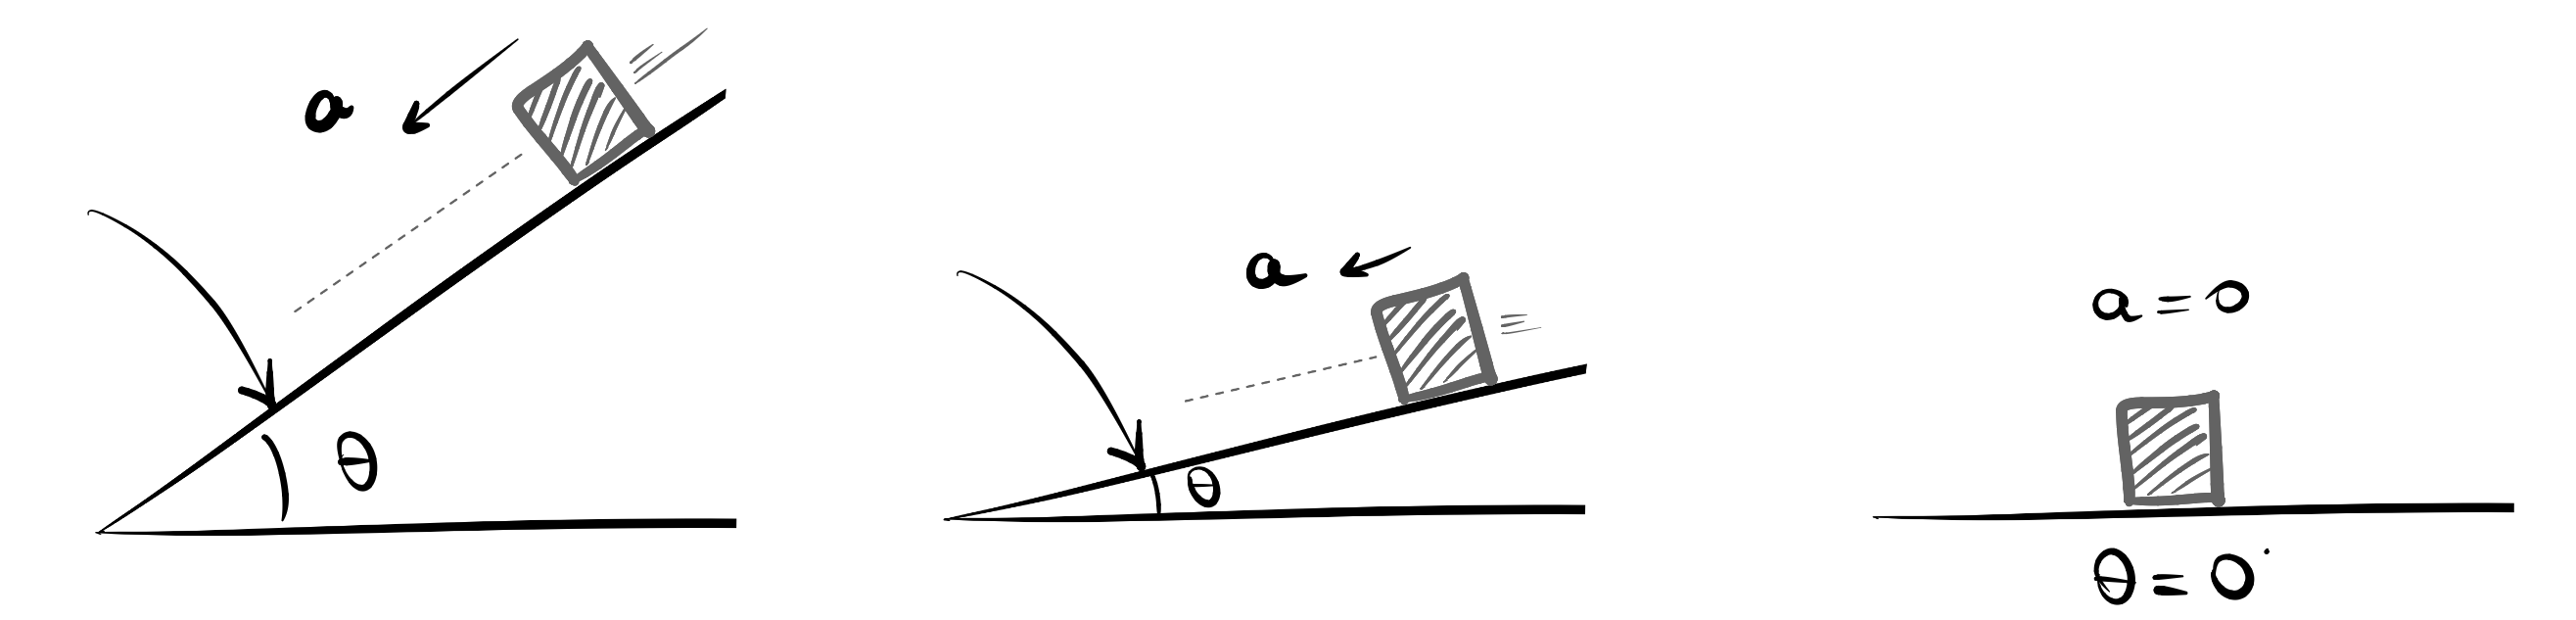
\includegraphics[width=0.8\linewidth]{imagensdinamicanewton/gsinthetacasoparticular1.png}};
  \end{scope}
\end{tikzpicture}
\captionof{figure}{Ao diminuir a inclinação do plano a aceleração da caixa deve diminuir, até zerar quando a inclinação do plano for nula.}
\label{fig_dinamicanewton_gsinthetacasoparticular1}
} 
\vspace{0.3cm}

Considere, por exemplo, a Figura \ref{fig_dinamicanewton_gsinthetacasoparticular1}. Nela, a cada nova etapa, o ângulo de inclinação do plano diminui. Isso faz com que a aceleração diminua e, no caso limite, quando deitarmos totalmente o plano e o ângulo for zero, o corpo estará em repouso: sua aceleração será nula. Ou seja, estamos dizendo que se $\theta =0,$ então devemos ter $a=0,$ uma vez que o corpo estará em um plano horizontal. Isso de fato ocorre, uma vez que $\sin 0 = 0,$ logo:

$$ a= g \sin 0 = 0.$$

\vspace{0.3cm}
{
\centering
\begin{tikzpicture}
  \begin{scope}[blend mode=multiply]
    \node {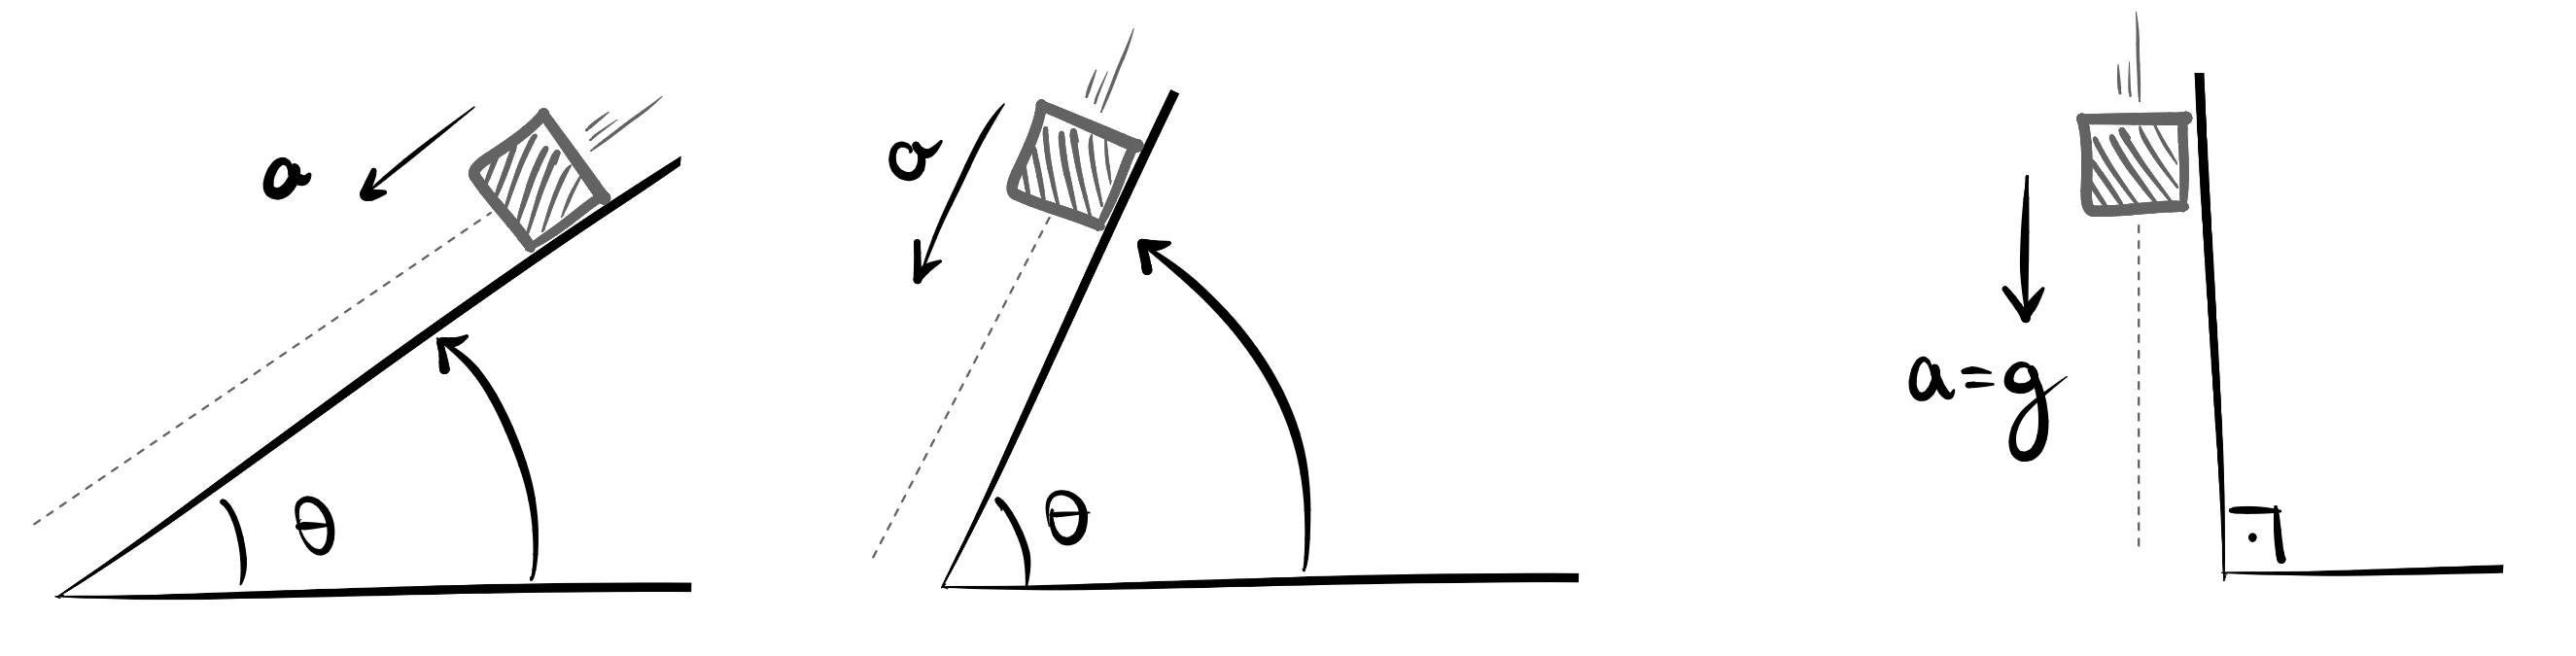
\includegraphics[width=0.8\linewidth]{imagensdinamicanewton/gsinthetacasoparticular2.png}};
  \end{scope}
\end{tikzpicture}
\captionof{figure}{Ao aumentar a inclinação do plano a aceleração da caixa deve aumentar, até atingir o valor máximo igual ao da gravidade quando a inclinação do plano for perpendicular ao chão.}
\label{fig_dinamicanewton_gsinthetacasoparticular2}
} 
\vspace{0.3cm}

Considere agora a situação da Figura \ref{fig_dinamicanewton_gsinthetacasoparticular2}. Neste caso tomamos o caminho oposto: vamos aumentar a inclinação do plano. Isso nos leva a crer que a aceleração irá aumentar, até atingir o seu valor máximo quando a inclinação do plano for de $90^\circ$: neste caso a caixa estará em queda livre, sendo sua aceleração, portanto, igual à da gravidade. Veja que é exatamente isso que a Equação \eqref{eq_dinamicanewtoniana_gsintheta} diz para $\theta=90^\circ$, uma vez que neste valor o seno é igual a 1:

$$ a = g \sin \left(\dfrac{\pi}{2}\right) = g.$$



Essa observação serve, talvez, para dois objetivos principais:

\begin{enumerate}
    \item [(i)] Mostrar que a Equação \eqref{eq_dinamicanewtoniana_gsintheta} serve para quaisquer valores de $\theta,$ ainda para situações que aparentavam não estar cobertas por ela: um plano horizontal com uma caixa em repouso ou um plano totalmente na vertical com uma caixa em queda livre.
    \item [(ii)] Evidenciar o motivo da estrutura da Equação \eqref{eq_dinamicanewtoniana_gsintheta} ser exatamente aquela. Perceba que se tivéssemos um cosseno no lugar do seno as conclusões que tiramos anteriormente não seriam corretas, o que mostraria que a equação deve estar errada. 
    
    Chamamos essa situação de análise de casos particulares: avaliamos uma equação que, a priori, vale para qualquer ângulo $\theta$, para dois valores bem específicos, no caso $\theta=0$ e $\theta = \sfrac{\pi}{2}.$ Fizemos isso porque esses dois casos particulares forneciam situações que nos eram familiares, de modo que poderíamos atestar se a tal equação de fato nos levaria ao que esperaríamos em tais situações -- o que de fato ocorre. Isso não prova que a equação está correta, é claro. Mas prova que ela, pelo menos, está de acordo com o que esperaríamos para algumas situações limite. \\
    Esse tipo de análise pode ajudar o leitor a se lembrar rapidamente da estrutura de uma equação que ele eventualmente tenha se esquecido, sem precisar, necessariamente, deduzir a equação do zero. Pode servir também para testar se uma equação encontrada está de fato correta: se ela não nos fornecer a resposta que esperamos para os casos mais simples, certamente ela está incorreta.
 \end{enumerate}

\vspace{0.3cm}

\begin{exemplo}[Nível I]\label{exemplo_dinamica1_planoinclinado01}

Um bloco é lançado com velocidade $v_0=30$ m/s de modo a subir um plano inclinado que faz um ângulo $\theta = 30^\circ$ com a horizontal.

Qual é a distância máxima que tal bloco sobe ao longo do plano?

\resolucao

A aceleração do bloco pode ser obtida pela aplicação direta da Equação \eqref{eq_dinamicanewtoniana_gsintheta} (o que eu farei, mas não recomendo que o leitor o faça, haja vista o conselho dado na subseção \textbf{Erros Comuns} sobre essa equação), de modo que o seu valor é

$$ a = g \sin \theta = 10 \cdot \sin 30^\circ = 5 \text{m/s}^2.$$

Computada a aceleração, daqui em diante torna-se um problema de Cinemática. Perceba que o valor da aceleração é constante, de modo que temos um MUV. Assim, podemos usar, por exemplo, a Equação de Torricelli:


$$ v^2 = v_0^2-2a\Delta s \implies \cancelto{0}{v^2} = 30^2 - 2 \cdot 5\Delta s \implies \Delta s = 90 \text{ m},$$

\noindent em que a velocidade final do bloco é zero uma vez que, tendo sido totalmente decelerado, ele começará a descer ao longo do plano. Assim, a máxima distância que ele sobe ao longo do plano é aquela que ele percorre até sua velocidade zerar.


\end{exemplo}


\vspace{0.3cm}


\begin{exemplo}[Nível II]\label{exemplo_dinamica1_planoinclinado02}

Considere um plano inclinado de inclinação $\theta$ em relação à horizontal e de massa $M,$ que pode se mover livremente, sem atrito, ao longo do solo. 

\vspace{0.3cm}
{
\centering
\begin{tikzpicture}
  \begin{scope}[blend mode=multiply]
    \node {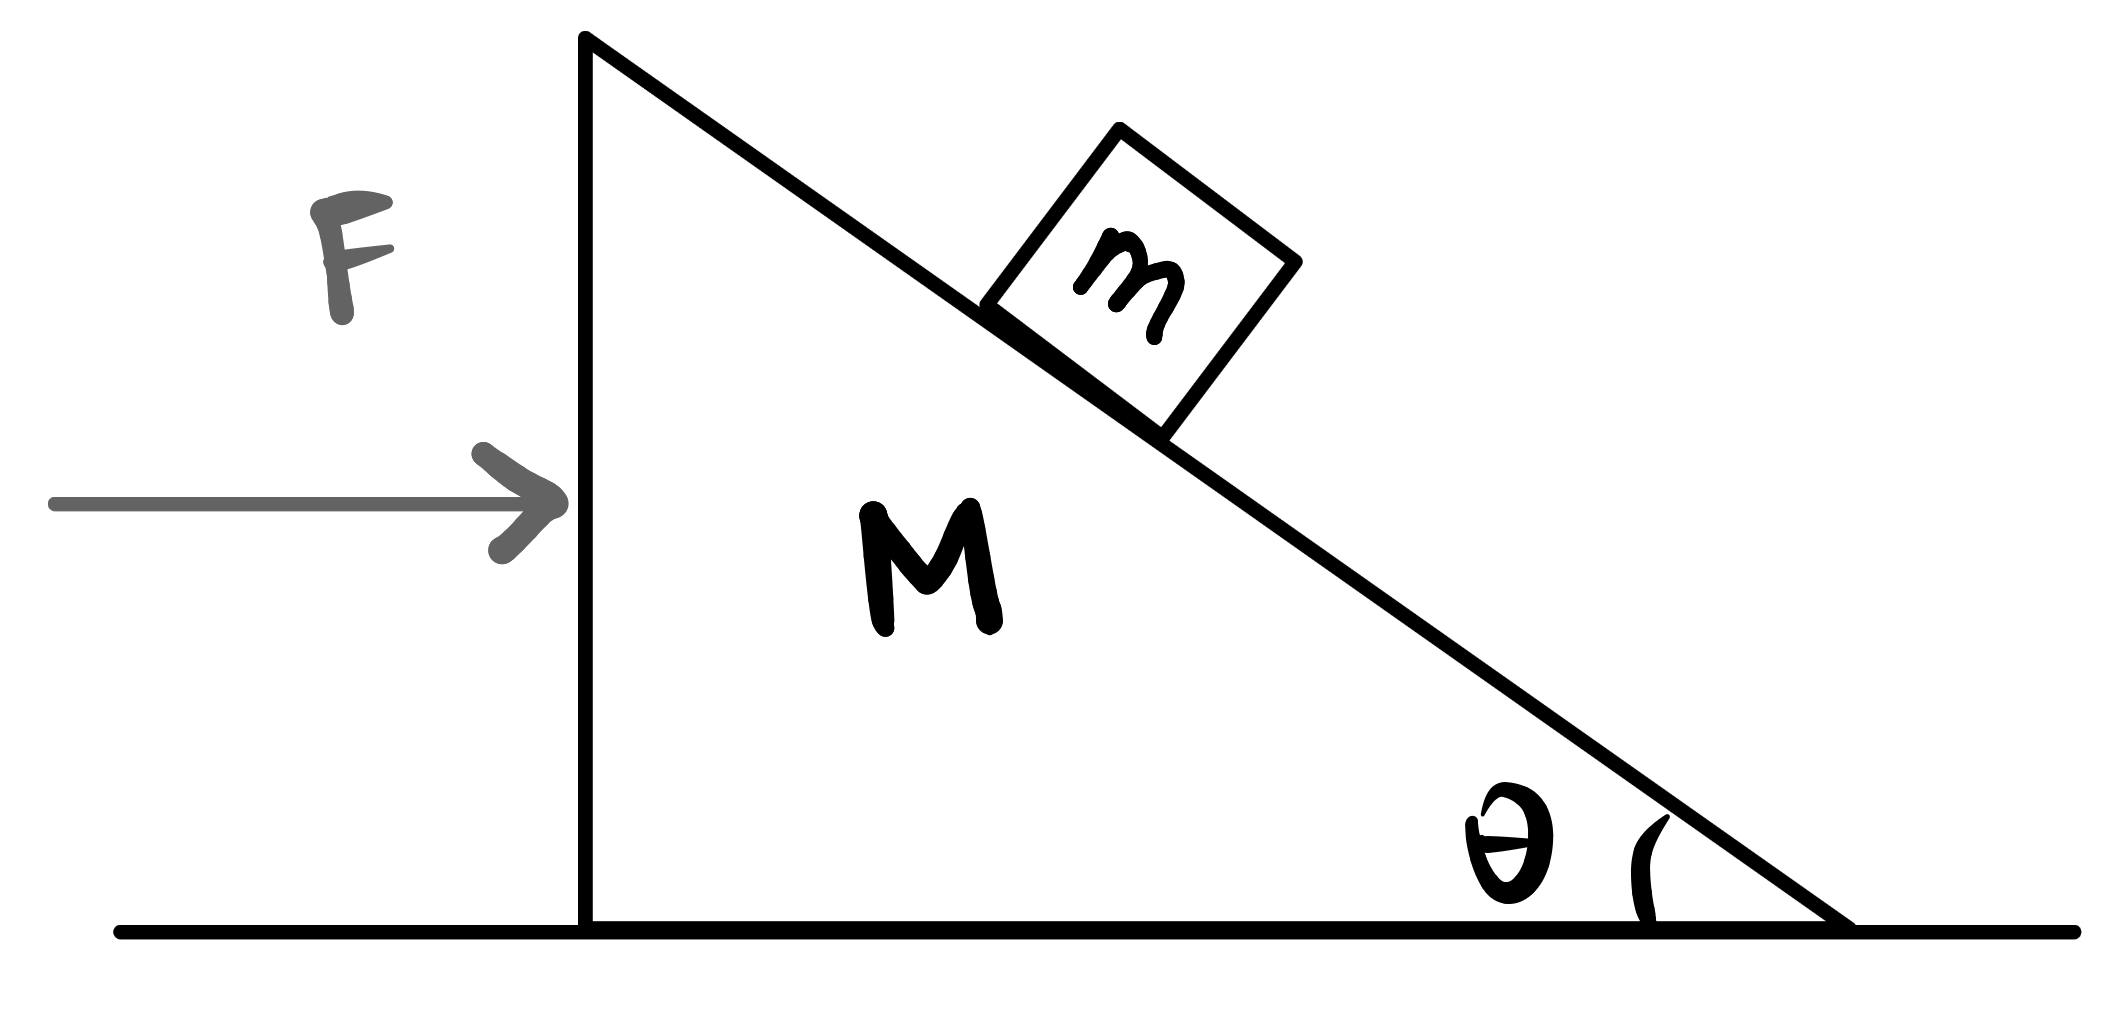
\includegraphics[width=0.35\linewidth]{imagensdinamicanewton/planoinclinadoexemplo2blocoerampa1.png}};
  \end{scope}
\end{tikzpicture}
\captionof{figure}{}
\label{fig_dinamicanewton_planoinclinadoexemplo2blocoerampa1}
} 
\vspace{0.3cm}

Em cima dele coloca-se um bloquinho de massa $m$, que também pode se mover livremente, sem atrito, ao longo do plano. Uma força $F$ é feita no plano e o acelera de tal modo que o bloquinho não se move em relação ao plano. Encontre o valor de $F.$

\resolucao

Podemos começar enxergando os dois corpos como um único corpo de massa $(m+M),$ uma vez que eles se moverão juntos, como se fosse um só corpo. 

\vspace{0.3cm}
{
\centering
\begin{tikzpicture}
  \begin{scope}[blend mode=multiply]
    \node {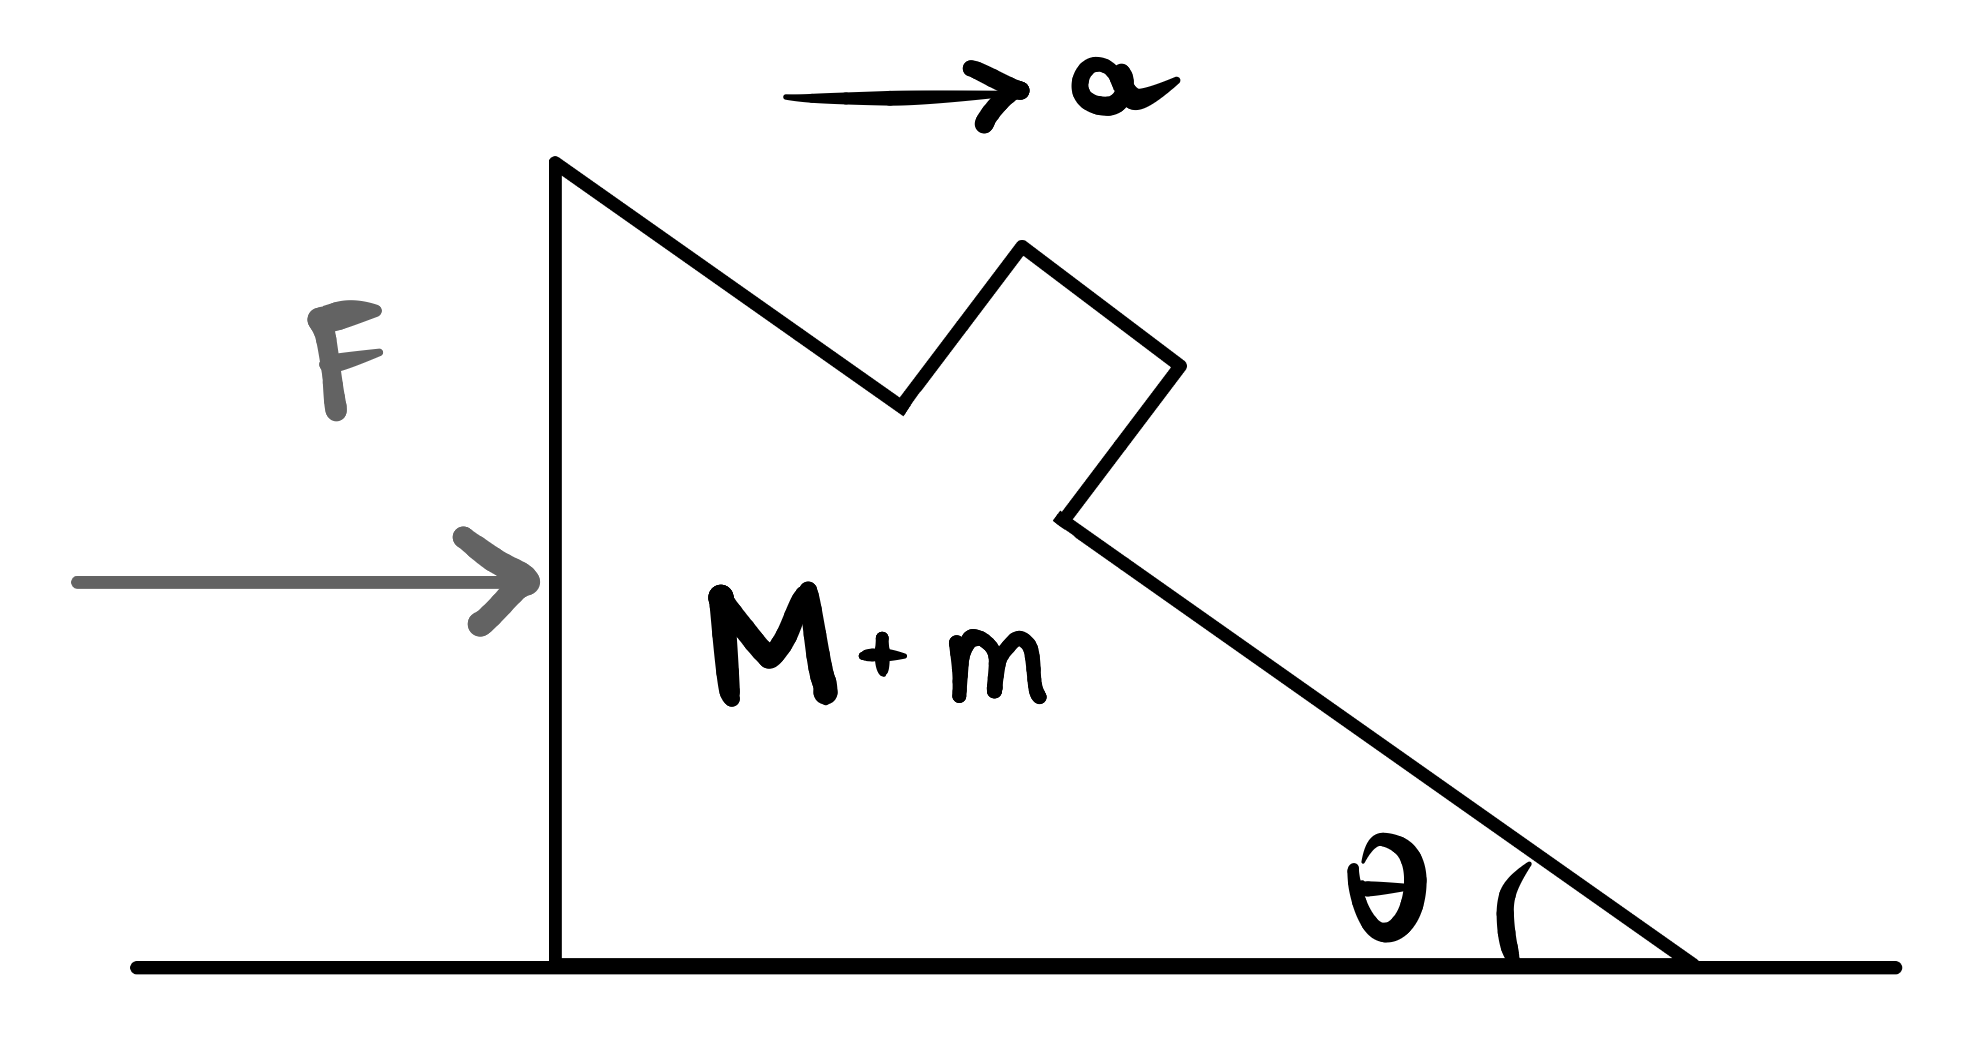
\includegraphics[width=0.35\linewidth]{imagensdinamicanewton/planoinclinadoexemplo2blocoerampa3.png}};
  \end{scope}
\end{tikzpicture}
\captionof{figure}{A rampa+bloco pode ser considerado como um corpo único.}
\label{fig_dinamicanewton_planoinclinadoexemplo2blocoerampa3}
} 
\vspace{0.3cm}


Neste caso, a força externa que acelera este sistema é a força horizontal $F$, de modo que a Segunda Lei de Newton se escreve como

$$ \boxed{F=(m+M)a.}$$

Agora, analisando separadamente as forças que atuam em cada bloco, avaliemos a resultante das forças no bloco de massa $m.$ A Figura \ref{fig_dinamicanewton_planoinclinadoexemplo2blocoerampa2} ilustra essa situação. Note que, para o bloco de massa $m,$ como ele acelera (e se move) horizontalmente para a direita, um dos eixos de decomposição das forças deverá ser o eixo horizontal -- sempre paralelo ao movimento do bloco. O outro eixo, sendo perpendicular ao primeiro, será o eixo vertical $y,$ como mostra a segunda imagem da Figura.


\vspace{0.3cm}
{
\centering
\begin{tikzpicture}
  \begin{scope}[blend mode=multiply]
    \node {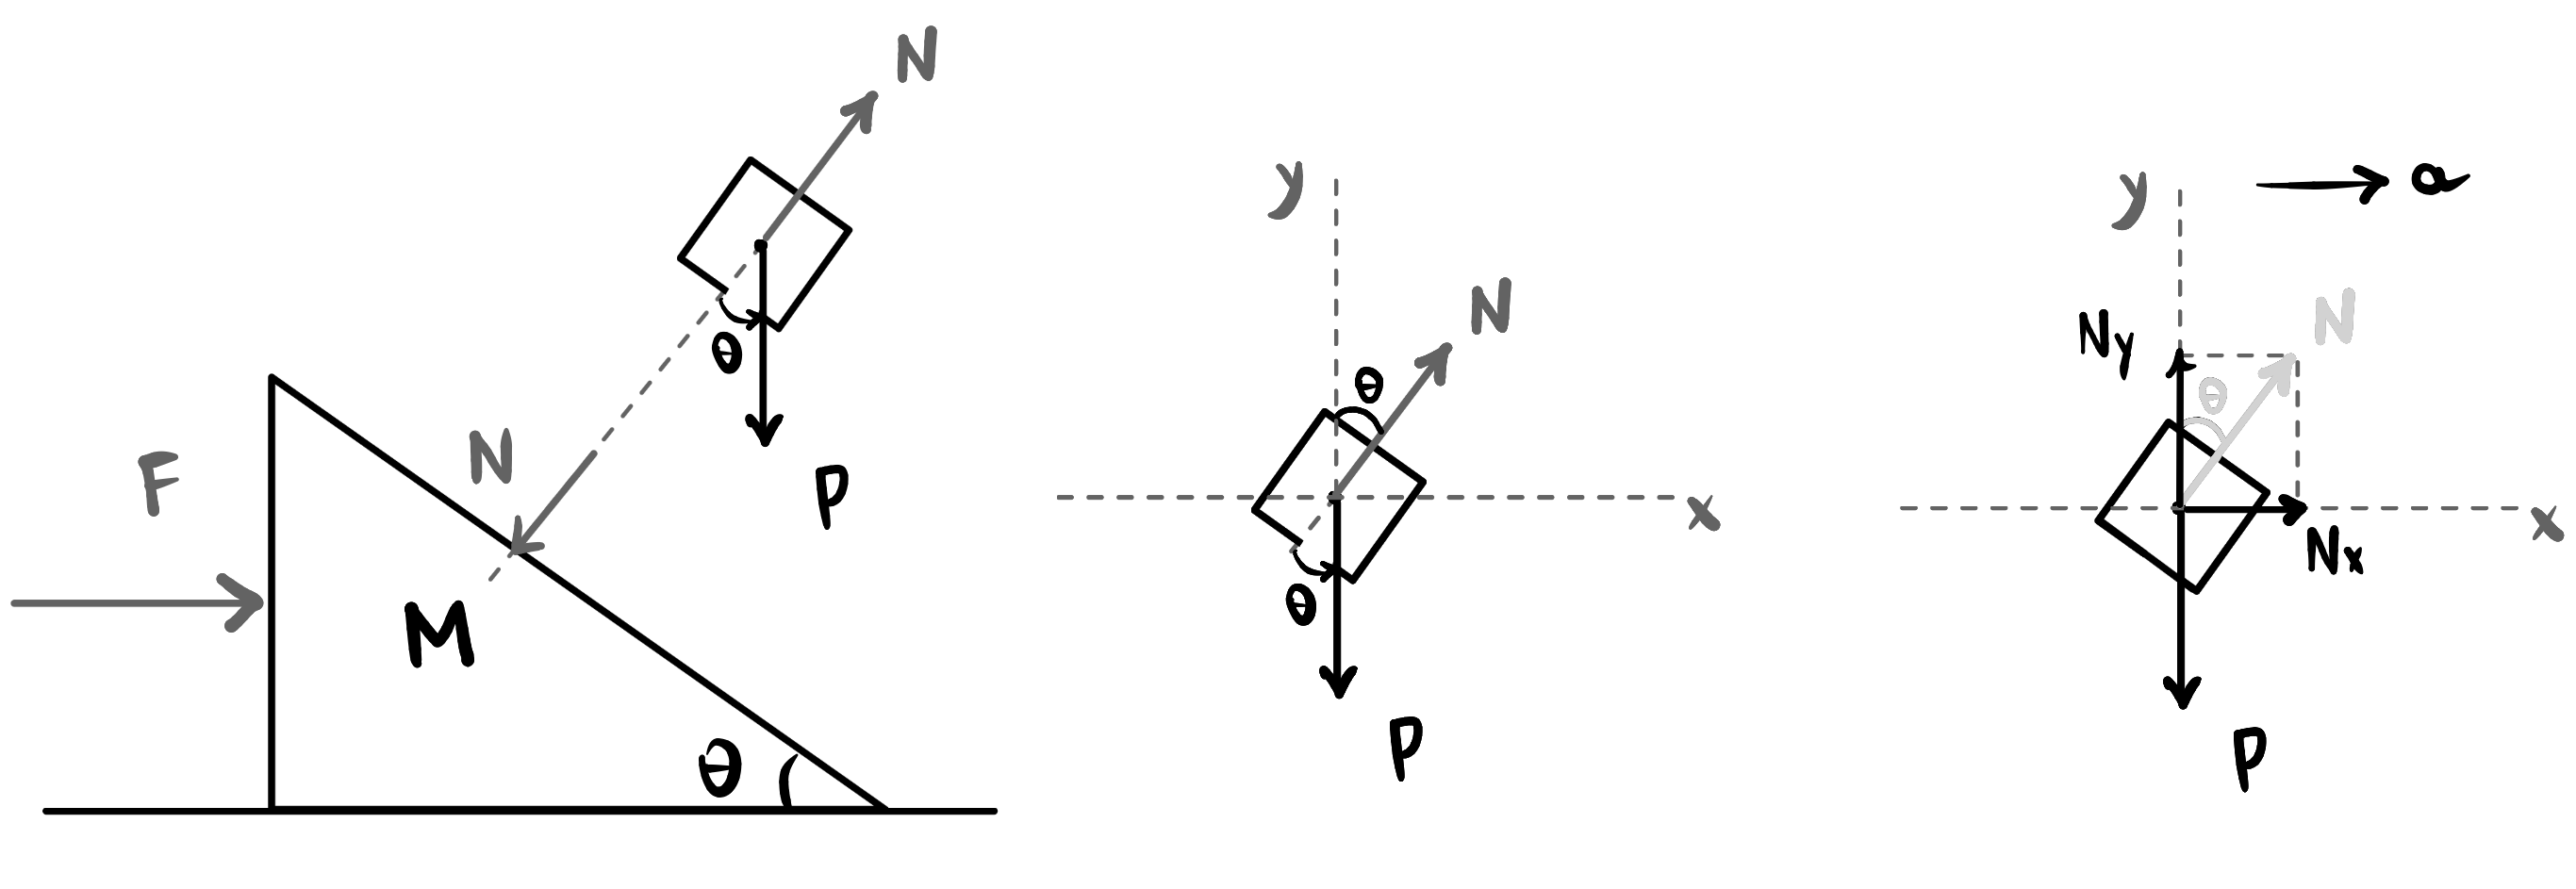
\includegraphics[width=0.95\linewidth]{imagensdinamicanewton/planoinclinadoexemplo2blocoerampa2.png}};
  \end{scope}
\end{tikzpicture}
\captionof{figure}{}
\label{fig_dinamicanewton_planoinclinadoexemplo2blocoerampa2}
} 
\vspace{0.3cm}

Assim, para o bloco de massa $m$, a Segunda Lei de Newton se escreve como:

$$
\begin{cases}
    F_{\text{R}x} = ma_x \implies N \sin \theta = ma \\
    F_{\text{R}y} = m \cancelto{0}{a_y  } =0\implies N \cos \theta = mg.
\end{cases}
$$

Dividindo as duas equações acima membro a membro, somos levados a

$$ \dfrac{\cancel N \sin \theta}{\cancel N \cos \theta} = \dfrac{\cancel ma}{\cancel mg} \implies \boxed{a = g \tan \theta.}$$

Ou seja, essa deve ser a aceleração \emph{exata} que o sistema deve ter para que o bloco de massa $m$ consiga se mover junto da rampa, sem escorregar em relação a ela.

Assim, da primeira relação obtida, é possível obter a força $F$ que viabiliza com que isso ocorra:

$$ F = (m+M)a \implies \boxed{F = (m+M)g \tan \theta.}$$
\end{exemplo}

\vspace{0.3cm}


\begin{exemplo}[Nível III]\label{exemplo_dinamica1_planoinclinado03}

Considere um plano inclinado de inclinação $\theta$ em relação à horizontal e de massa $M,$ que pode se mover livremente, sem atrito, ao longo do solo. Em cima dele coloca-se um bloquinho de massa $m$, que também pode se mover livremente, sem atrito, ao longo do plano. Ao abandonar o bloquinho, encontre o valor da aceleração do plano em relação à Terra.

\resolucao

A complexidade deste problema está no fato de que o plano
inclinado se move, de modo que não podemos simplesmente decompor o
peso do bloquinho ao longo do plano como faríamos num plano fixo. A Figura \ref{fig_dinamicanewton_planoinclinadoescorregandoex3nivelita1} ilustra essa situação: quando o bloco começa escorregar plano abaixo, o plano começa a recuar para a esquerda, com aceleração $A$. Isso faz com que, em relação à Terra, a trajetória do bloco não seja paralela ao plano inclinado.
% saída é trabalhar com as acelerações absolutas (em relação à Terra) e
% aplicar a Segunda Lei a cada corpo separadamente.

\vspace{0.3cm}
{
\centering
\begin{tikzpicture}
  \begin{scope}[blend mode=multiply]
    \node {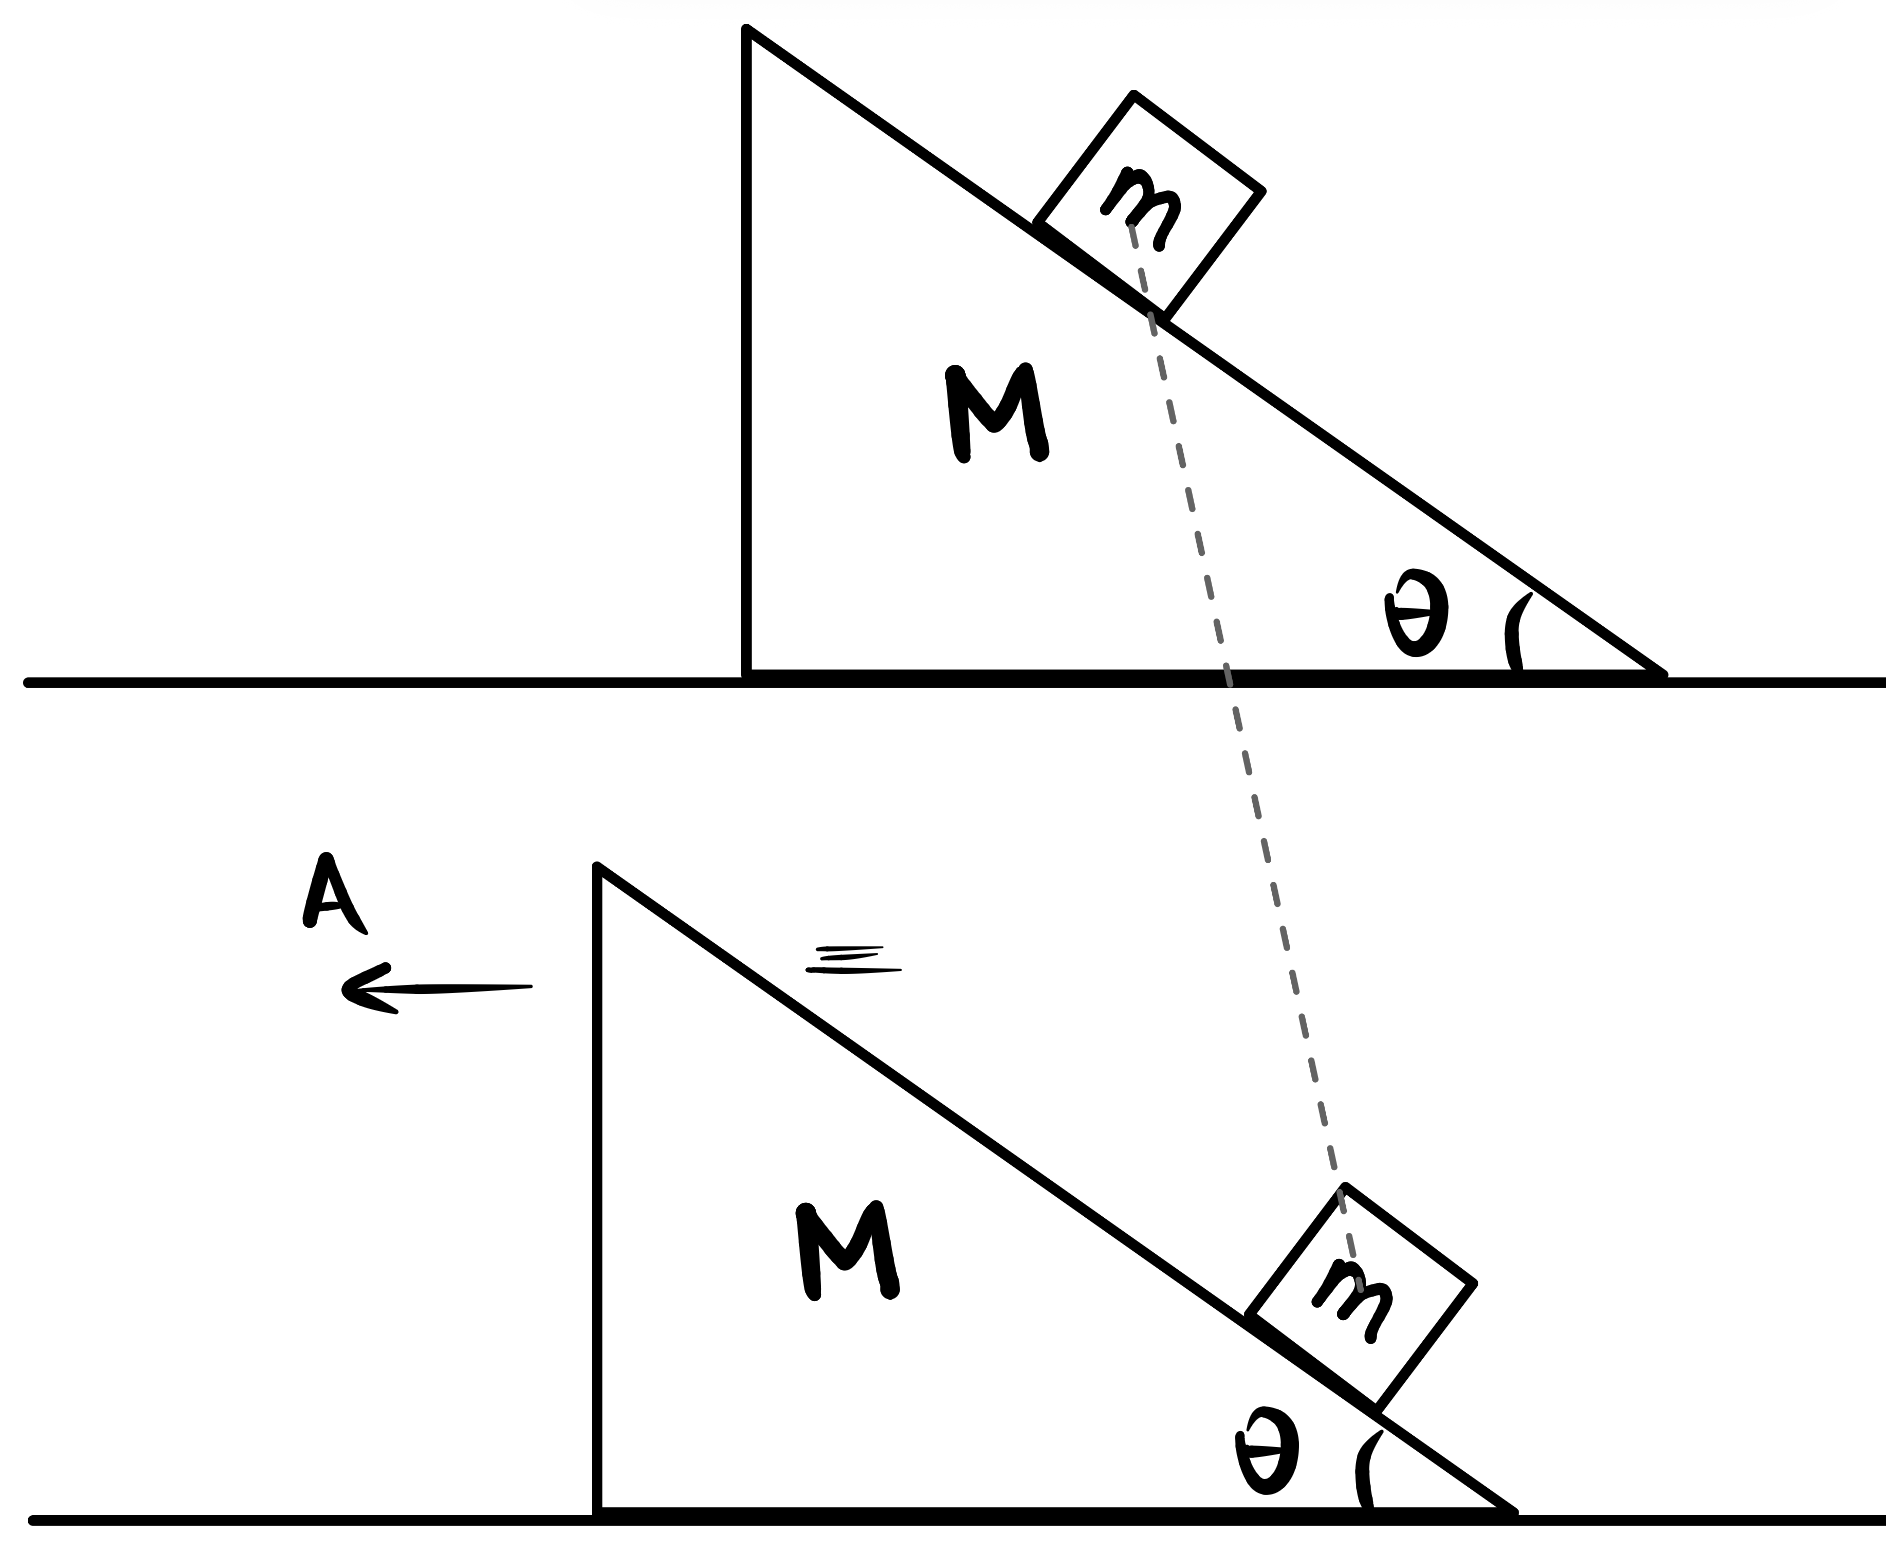
\includegraphics[width=0.45\linewidth]{imagensdinamicanewton/planoinclinadoescorregandoex3nivelita1.png}};
  \end{scope}
\end{tikzpicture}
\captionof{figure}{}
\label{fig_dinamicanewton_planoinclinadoescorregandoex3nivelita1}
} 
\vspace{0.3cm}

No referencial do plano o bloco, naturalmente, se move na direção do plano inclinado. Seja $a$ a aceleração do bloco no referencial do plano. Ela possui componentes $a_x$ e $a_y$, representadas na Figura \ref{fig_dinamicanewton_planoinclinadoescorregandoex3nivelita2}.

\vspace{0.3cm}
{
\centering
\begin{tikzpicture}
  \begin{scope}[blend mode=multiply]
    \node {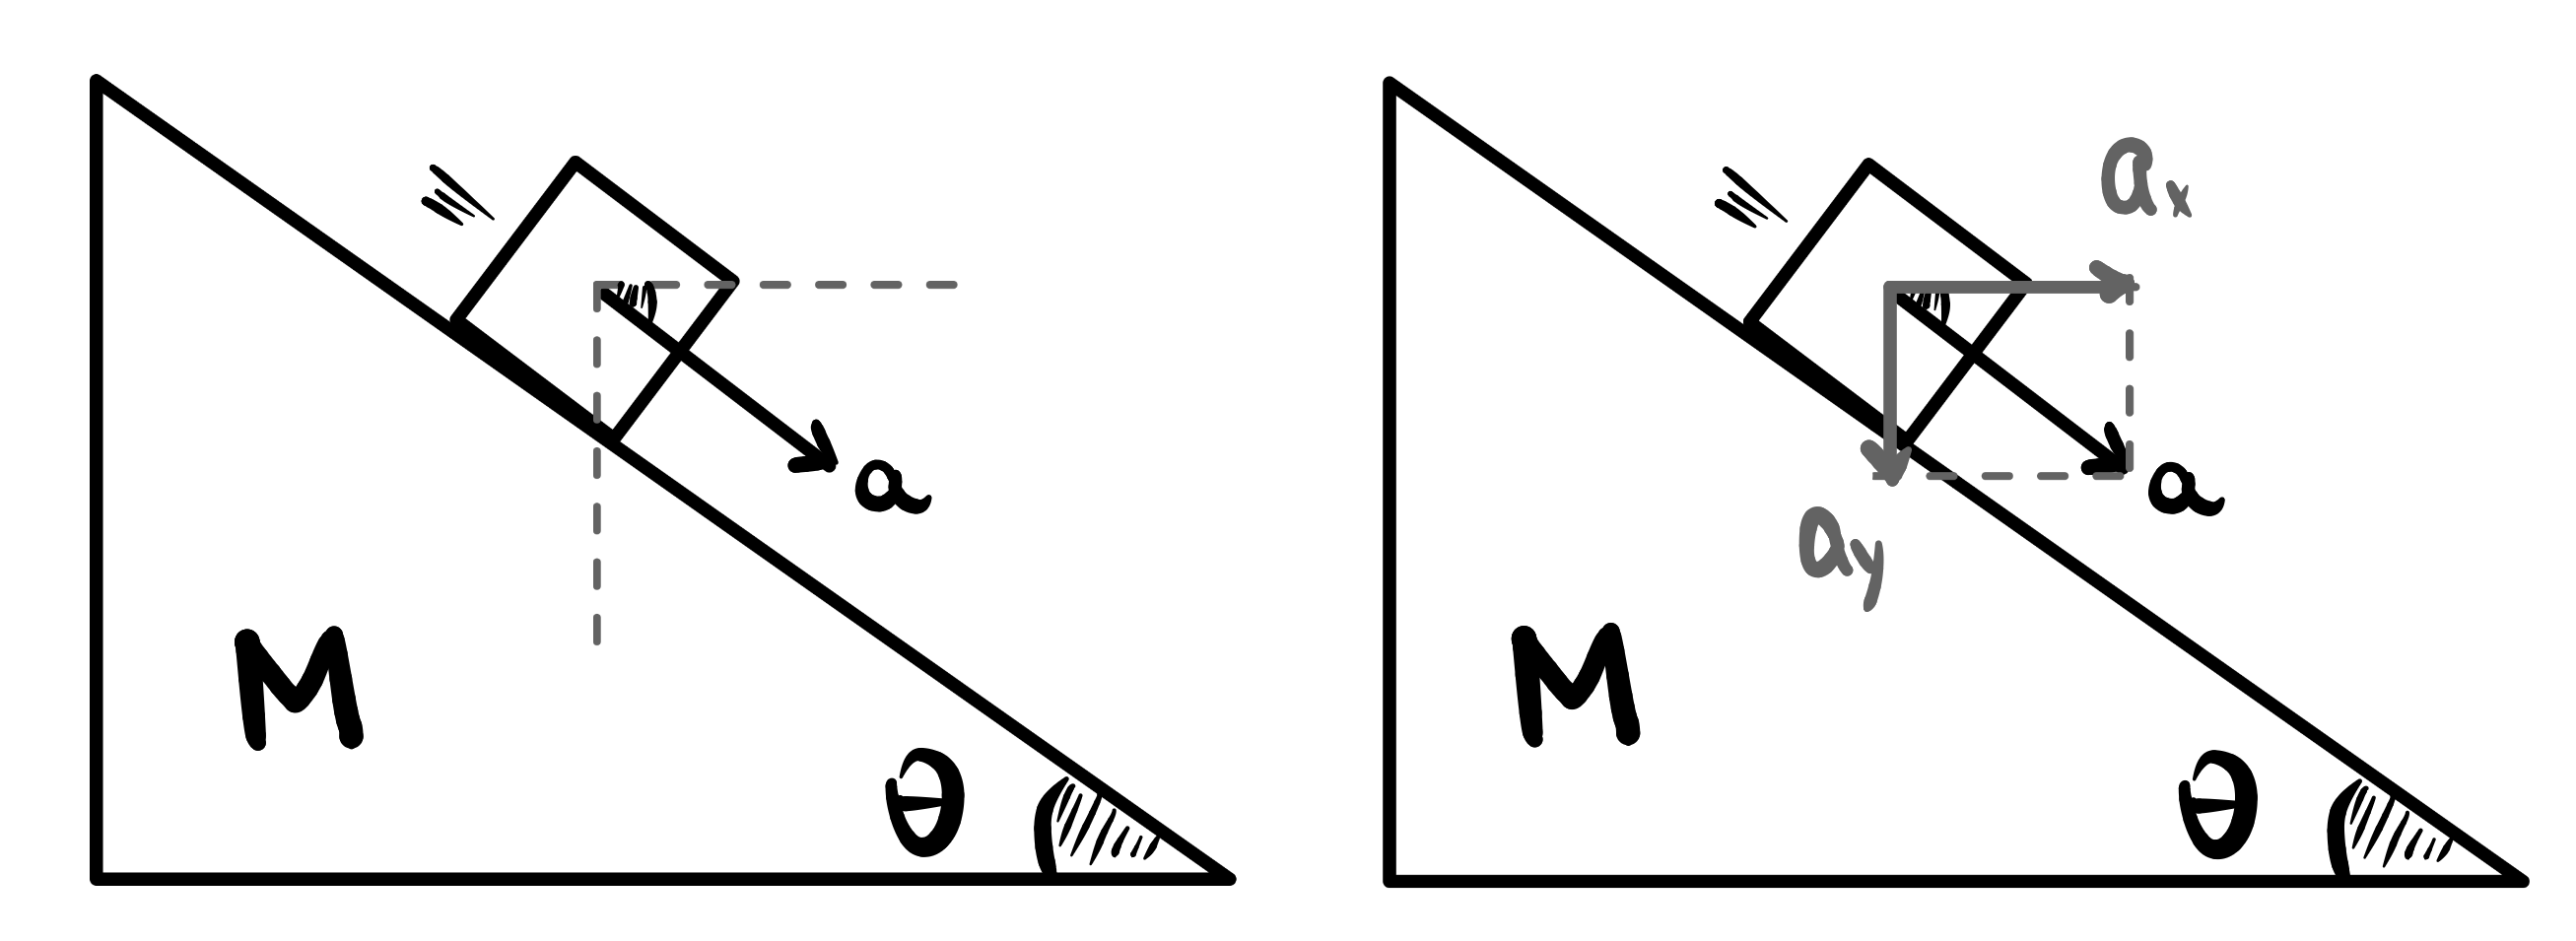
\includegraphics[width=0.55\linewidth]{imagensdinamicanewton/planoinclinadoescorregandoex3nivelita2.png}};
  \end{scope}
\end{tikzpicture}
\captionof{figure}{}
\label{fig_dinamicanewton_planoinclinadoescorregandoex3nivelita2}
} 
\vspace{0.3cm}


Sendo $A$ a aceleração do plano em relação à Terra (horizontal, para a
esquerda --- pois o bloco empurra o plano nessa direção ao deslizar).
Então a aceleração absoluta do bloquinho em relação à terra tem então:

\begin{itemize}
  \item componente horizontal: $a\cos\theta - A$ (para a direita);
  \item componente vertical: $-a\sin\theta$ (para baixo).
\end{itemize}

\medskip

A única força de contato entre o bloco e o plano é a normal $N$,
perpendicular à superfície da rampa. Ela aponta para cima e para a
direita sobre o bloco; para baixo e para a esquerda sobre o plano
(Terceira Lei). A Figura \ref{fig_dinamicanewton_planoinclinadoescorregandoex3nivelita3} mostra o diagrama de forças para cada um dos dois corpos.

\vspace{0.3cm}
{
\centering
\begin{tikzpicture}
  \begin{scope}[blend mode=multiply]
    \node {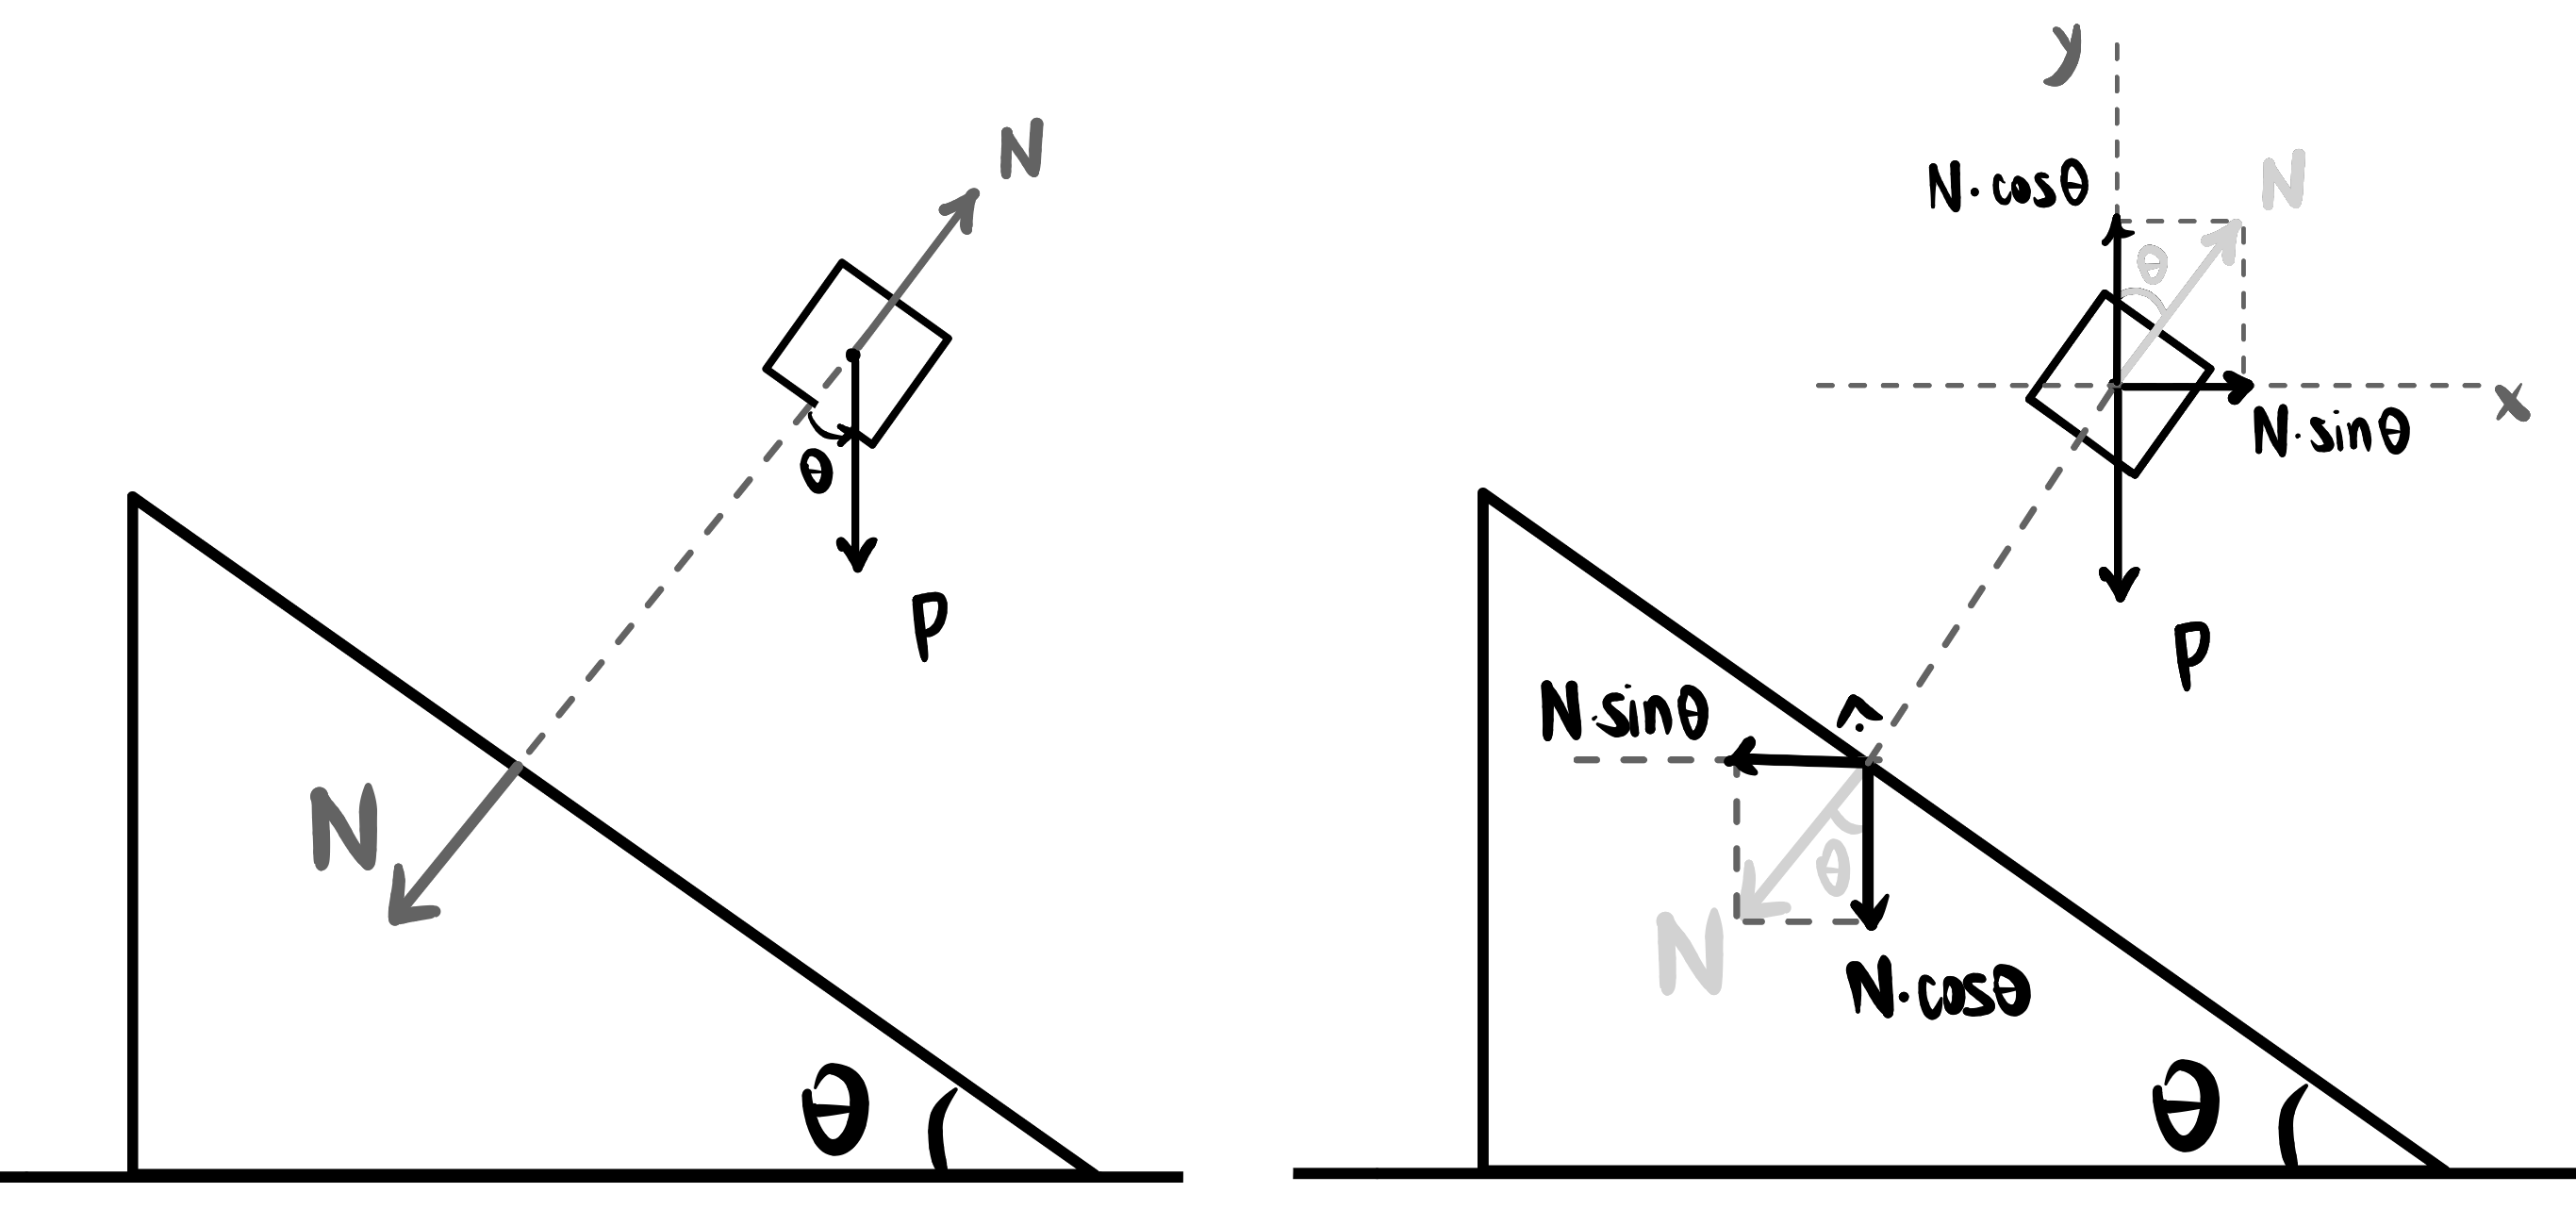
\includegraphics[width=0.8\linewidth]{imagensdinamicanewton/planoinclinadoescorregandoex3nivelita3.png}};
  \end{scope}
\end{tikzpicture}
\captionof{figure}{}
\label{fig_dinamicanewton_planoinclinadoescorregandoex3nivelita3}
} 
\vspace{0.3cm}


\medskip
Equacionando a Segunda Lei em $x$ e $y$ para o bloquinho, ter-se-á:

\begin{align}
  N\sin\theta &= m(a\cos\theta - A), \tag{1} \\
  N\cos\theta - mg &= -ma\sin\theta. \tag{2}
\end{align}

Para o plano inclinado (só a direção horizontal importa, pois ele não sai do solo):

\[
  N\sin\theta = MA. \tag{3}
\]

\medskip
De (1) e (3):

\[
  MA = m(a\cos\theta - A)
  \;\Longrightarrow\;
  A(M+m) = ma\cos\theta
  \;\Longrightarrow\;
  A = \frac{ma\cos\theta}{M+m}. \tag{4}
\]

De (2):

\[
  N = \frac{m(g - a\sin\theta)}{\cos\theta}. \tag{5}
\]

De (3) e (4):

\[
  N = \frac{MA}{\sin\theta} = \frac{Mma\cos\theta}{(M+m)\sin\theta}. \tag{6}
\]

Igualando (5) e (6):

\[
  \frac{m(g - a\sin\theta)}{\cos\theta}
  = \frac{Mma\cos\theta}{(M+m)\sin\theta}.
\]

Multiplicando ambos os lados por $\cos\theta\cdot(M+m)\sin\theta$:

\[
  (g - a\sin\theta)(M+m)\sin\theta = Ma\cos^2\theta,
\]
\[
  g(M+m)\sin\theta
  = a\bigl[M\cos^2\theta + (M+m)\sin^2\theta\bigr]
  = a\bigl[M + m\sin^2\theta\bigr].
\]

Portanto:

\[
  a = \frac{g(M+m)\sin\theta}{M + m\sin^2\theta}.
\]

Substituindo em (4):

\[
  A = \frac{m\cos\theta}{M+m}
    \cdot \frac{g(M+m)\sin\theta}{M + m\sin^2\theta},
\]

\[
  \boxed{A = \frac{mg\sin\theta\cos\theta}{M + m\sin^2\theta}.}
\]

\medskip

Vamos verificar alguns casos limite para ver se a resposta faz sentido físico.

\begin{center}
\begin{tabular}{cll}
\toprule
\textbf{Caso limite} & \textbf{Resultado} & \textbf{Interpretação} \\
\midrule
$m \to 0$      & $A \to 0$ & Sem bloco, o plano não se move \\
$M \to \infty$ & $A \to 0$ & Plano infinitamente pesado, permanece fixo \\
$\theta = 0^\circ$  & $A = 0$   & Superfície plana, sem força horizontal \\
$\theta = 90^\circ$ & $A = 0$   & Bloco cai verticalmente, não empurra o plano \\
\bottomrule
\end{tabular}
\end{center}

\noindent O máximo de $A$ ocorre num ângulo intermediário: há um
$\theta^*$ que maximiza $\sin\theta\cos\theta\,/\,(M + m\sin^2\theta)$,
revelando que existe uma inclinação ótima para a qual o plano recua
mais rapidamente. O leitor consegue encontrar essa condição e achar $A_{MAX}?$

\medskip

Por fim, cabe comentarmos um outro tipo de solução para este mesmo problema, que reside em um certo \emph{vínculo} entre o movimento do bloco e da rampa: como o bloco sempre permanece em contato com a rampa isso significa que a aceleração relativa entre esses corpos na direção perpendicular à rampa é zero:


$$ A \sin \theta = a_x \sin \theta - a_y \cos \theta. \tag{7}$$

As Equações $(1)$ e $(2)$ são simplesmente a Segunda Lei de Newton para o bloquinho na horizontal e vertical, respectivamente. De onde tiramos que:

$$ N \sin \theta = ma_x \implies \boxed{a_x = \dfrac{N \sin \theta}{m},} \tag{8}$$

$$ N \cos \theta - mg = ma_y \implies \boxed{a_y = \dfrac{N \cos \theta  - mg}{m}.} \tag{9}$$


De $(3)$ extraímos que 

$$ A = \dfrac{N \sin \theta }{M} \tag {10}.$$

Substituindo (8), (9) e (10) na Equação do vínculo (7):


$$ \dfrac{N \sin \theta }{M} \sin \theta = \dfrac{N \sin \theta}{m} \sin \theta - \dfrac{(N \cos \theta  - mg)}{m}\cos \theta,$$

\noindent que, desenvolvendo, nos leva a

$$N = \frac{gmM\cos\theta}{M + m\sin^2\theta}.$$

Substituindo em (10):

$$\boxed{A = \frac{gm\sin\theta\cos\theta}{M + m\sin^2\theta}.}$$

A sacada dessa solução está no vínculo (7): ao exigir que a aceleração relativa não tenha componente normal, eliminamos completamente a aceleração relativa $a$ do sistema
--- ela sequer aparece. O problema se reduz a três equações de Newton em três incógnitas, e fecha direto.

\end{exemplo}



\begin{secnivel}[Condição de Equilíbrio]{I}{Condição de Equilíbrio}
  
  \eqLdois{def}{eq_newton_equilibriof=0}{F_R=0}

\end{secnivel}







\secgfe{De onde vem}

Vamos ampliar o nosso vocabulário: em Física, quando se diz que um corpo está em equilíbrio, queremos dizer que a resultante das forças que nele atuam é nula. Essa é uma definição: equilíbrio é a condição em que um corpo está tal que a Equação \eqref{eq_newton_equilibriof=0} é satisfeita.



\secgfe{Onde é usada}

Em diversos contextos iremos lidar com corpos em equilíbrio -- seja em repouso ou em MRU. O importante aqui é que o leitor esteja familiarizado com tal termo e entenda, fisicamente, o que isso significa. Ao se deparar com uma situação que diz que um certo corpo está em equilíbrio, a Equação \eqref{eq_newton_equilibriof=0} precisa vir na sua mente de imediato -- ela é versão matemática que define o que é a condição de equilíbrio.



\secgfe{Erros comuns}

O erro mais comum é assumir que, por estar em equilíbrio, o corpo tem que estar, necessariamente, parado. Como já vimos no estudo da Segunda Lei de Newton na Seção \ref{secao_mecanicanewtoniana_segundaleinewton}, diferente do que Aristóteles pensava, se a força resultante atuando em um corpo é nula, existem não apenas uma, mas duas situações que satisfazem tal condição:

\begin{enumerate}
    \item [(i)] Repouso.

     O corpo pode estar, de fato, parado. Chamamos essa condição de \textbf{equilíbrio estático}.

    \item [(ii)] Movimento Retilíneo Uniforme (MRU).

    Como observado por Galileu, existe um outro estado de movimento inercial além do repouso: o MRU -- um estado de movimento na ausência de forças. Assim, se $F_R=0,$ o corpo pode também estar em MRU, e permaneceria indefinidamente em tal estado a menos que uma força se manifeste para alterar seu estado de movimento. Isso é justamente o que diz a Primeira Lei de Newton.

    Tal condição é chamada de \textbf{equilíbrio dinâmico.}
\end{enumerate}



\secgfe{Observações}

Dentro da condição de equilíbrio estático, ou seja, quando já se sabe que o corpo está em repouso, existem algumas situações distintas que merecem ser destacadas. Considere a Figura \ref{fig_newton_equilibrioestavel1}, em que temos, nas três situações, a bolinha em equilíbrio estático.

\vspace{0.3cm}
{
\centering
\begin{tikzpicture}
  \begin{scope}[blend mode=multiply]
    \node {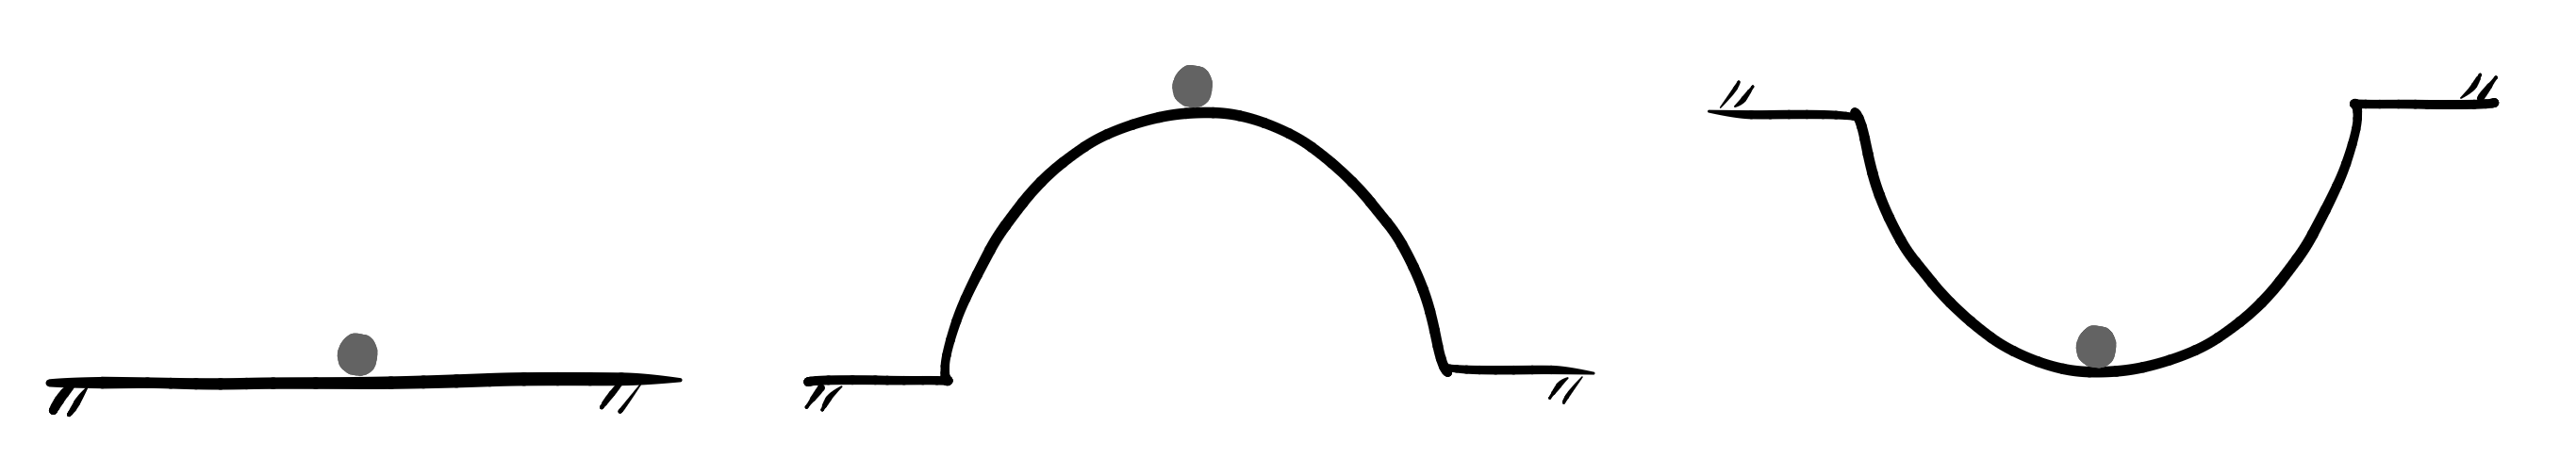
\includegraphics[width=0.8\linewidth]{imagensdinamicanewton/equilibrioestavel1.png}};
  \end{scope}
\end{tikzpicture}
\captionof{figure}{Três corpos em condição de equilíbrio estático.}
\label{fig_newton_equilibrioestavel1}
} 
\vspace{0.3cm}

Qual seria a diferença entre cada uma delas? Ora, se nas três situações trata-se de uma condição de equilíbrio, então certamente as forças atuantes precisam se anular. A Figura \ref{fig_newton_equilibrioestavel2} ilustra isso: por conta de seu peso a bolinha comprime o solo, fazendo nele uma força normal. Pela Terceira Lei o solo reage, fazendo uma força normal na bolinha, que deve ser anulada pelo seu peso, a fim de garantir a condição de equilíbrio.


\vspace{0.3cm}
{
\centering
\begin{tikzpicture}
  \begin{scope}[blend mode=multiply]
    \node {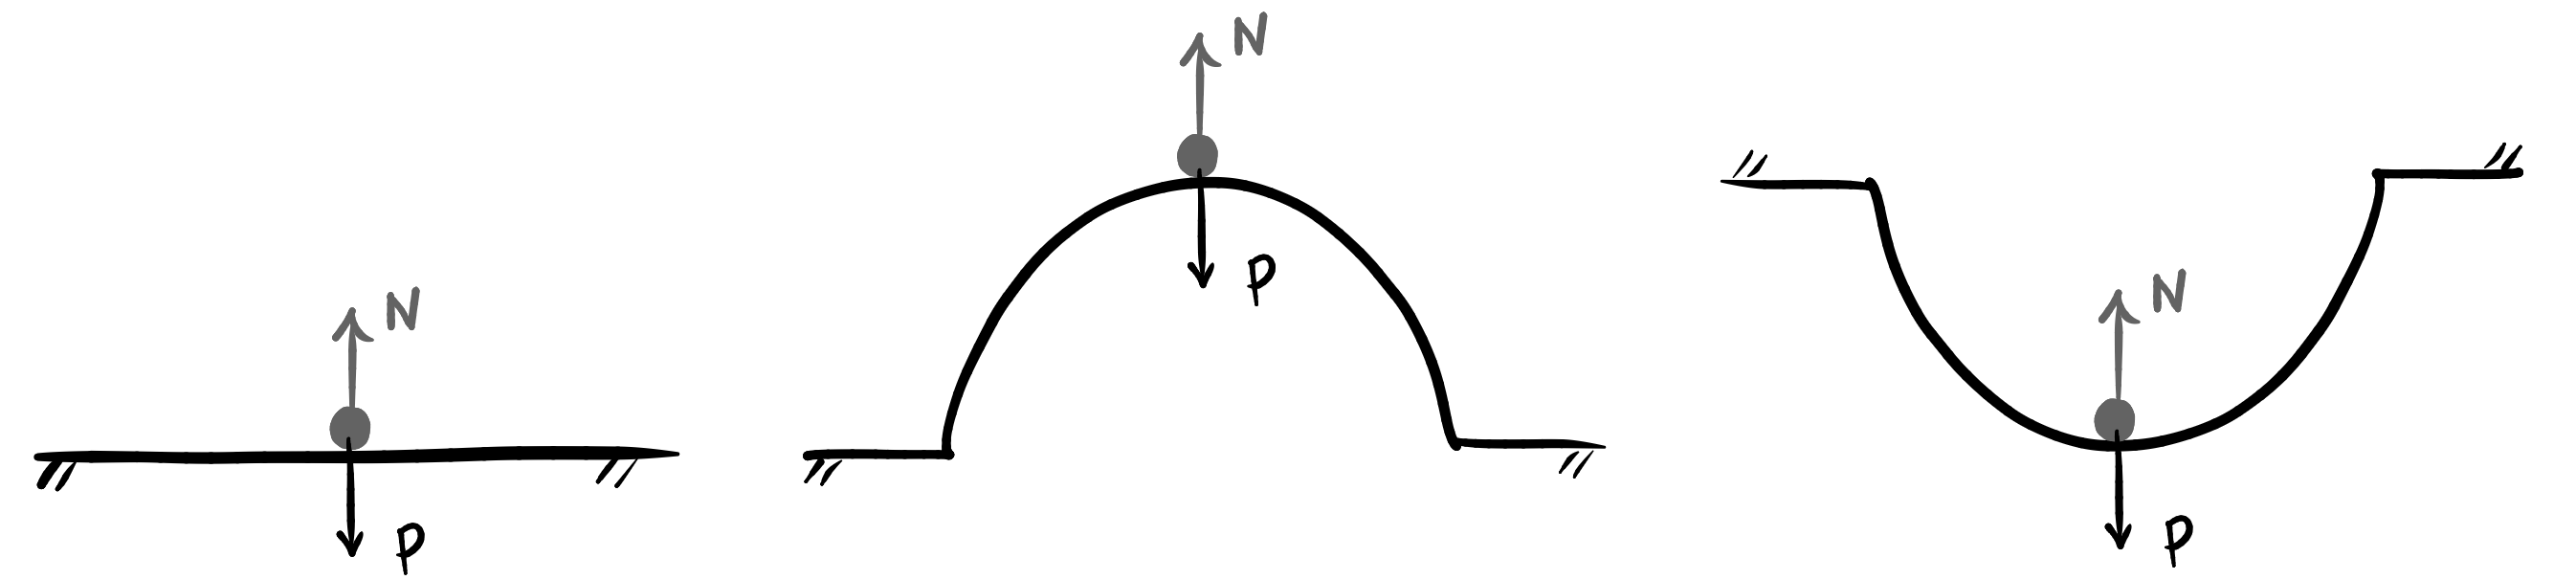
\includegraphics[width=0.8\linewidth]{imagensdinamicanewton/equilibrioestavel2.png}};
  \end{scope}
\end{tikzpicture}
\captionof{figure}{A condição de equilíbrio impõe que $F_R=0$, ou seja, a força normal anula o peso.}
\label{fig_newton_equilibrioestavel2}
} 
\vspace{0.3cm}

Note, contudo, que existe uma diferença entre as três situações da Figura \ref{fig_newton_equilibrioestavel1}. Não tem a ver com a dinâmica das forças, mas sim com o que acontece com o sistema ao ser levemente perturbado. Considere a situação de afastar levemente a bolinha da sua posição inicial de equilíbrio, isto é, retirá-la de onde ela está e colocá-la e uma posição, digamos, um centímetro para a direita. Na situação da primeira imagem ela voltaria a ficar em equilíbrio nessa mesma posição. Contudo, na situação da segunda imagem -- no topo do morro -- ao se deslocar de muito pouco para a direita a bolinha começaria a rolar morro abaixo. Tal situação é chamada, portanto, de \textbf{equilíbrio instável:} ao ser levemente perturbada da sua posição de equilíbrio a bolinha tende a se afastar de tal posição.

Já na situação da terceira imagem, no fundo do vale, ao se deslocar de muito pouco para a direita a bolinha começaria a rolar de volta para baixo, tendendo a volta para a sua posição anterior. Tal situação é chamada, portanto, de \textbf{equilíbrio estável:} ao ser levemente perturbada da sua posição de equilíbrio a bolinha tende a retornar para tal posição. Tal situação dará origem a movimentos oscilatórios, em que o corpo poderá oscilar em torno da sua posição de equilíbrio. 

A Figura \ref{fig_newton_rolypoly} ilustra um brinquedo, o \emph{João Bobo,} que representa bem a situação de equilíbrio estável: ao golpear e tombar o brinquedo ele sempre retorna à sua posição inicial de equilíbrio. Isso tem a ver com a posição do seu centro de massa, assunto que será discutido em detalhes no estudo da Equação \eqref{eq_newtonrotacao_posicaocentrodemassa}.

\vspace{0.3cm}
{
\centering
\begin{tikzpicture}
  \begin{scope}[blend mode=multiply]
    \node {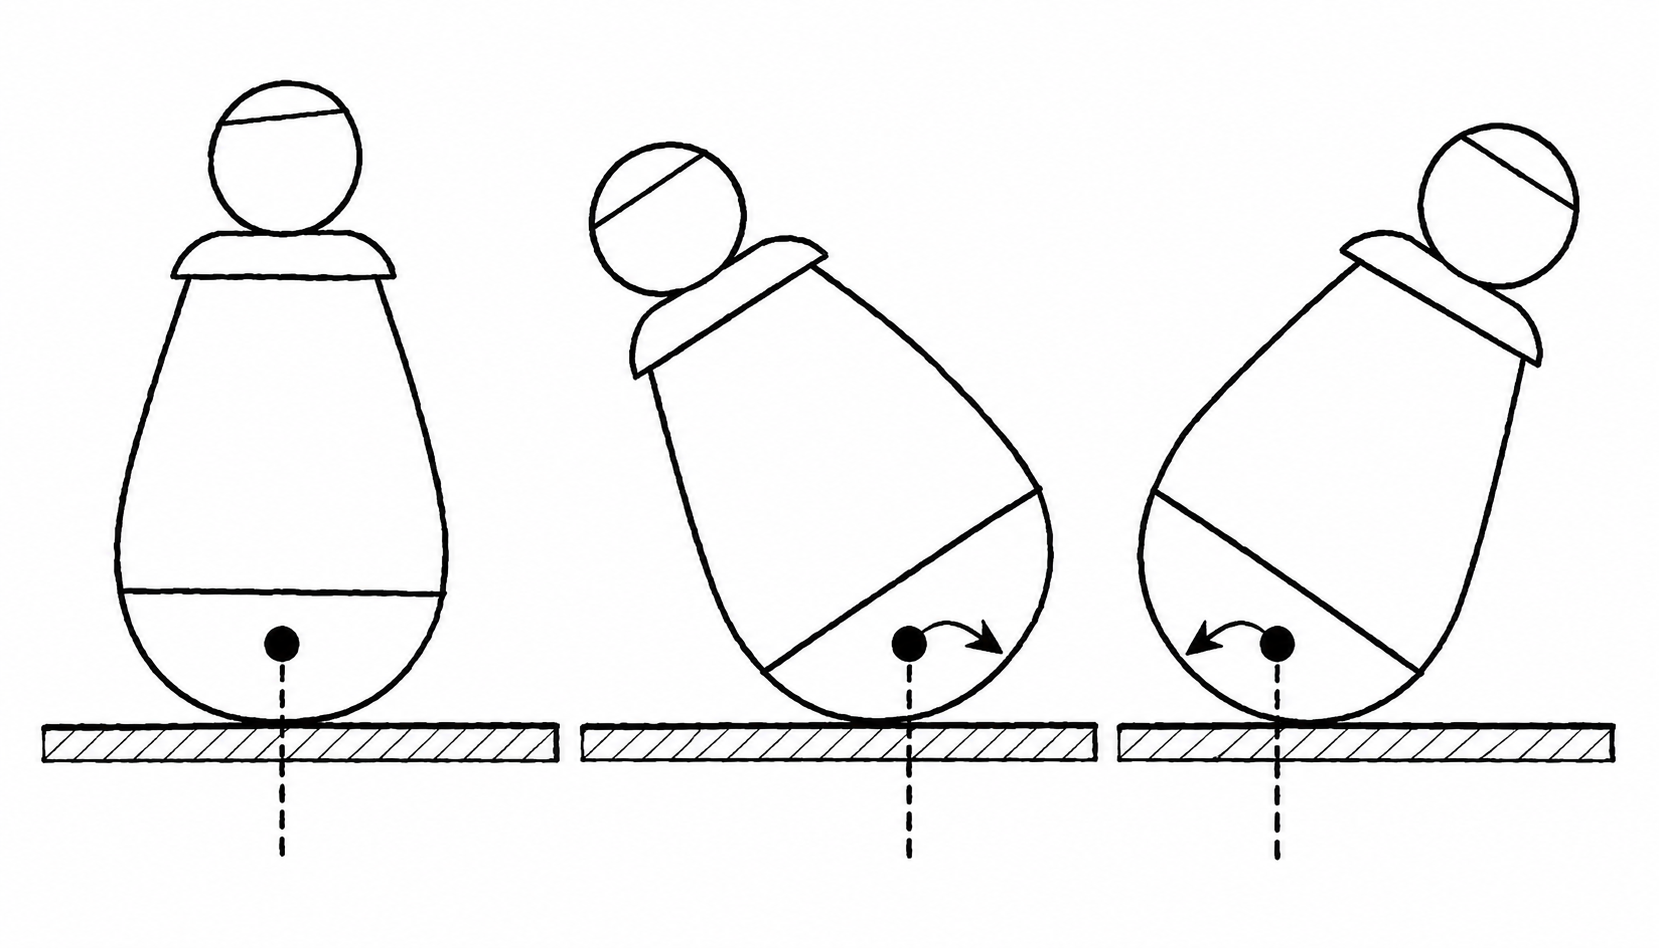
\includegraphics[width=0.5\linewidth]{imagensdinamicanewton/joaobobo.png}};
  \end{scope}
\end{tikzpicture}
\captionof{figure}{Brinquedo que ilustra a condição de equilíbrio estável.}
\label{fig_newton_rolypoly}
} 
\vspace{0.3cm}



Já a situação da primeira imagem é chamada de \textbf{equilíbrio indiferente}: o corpo não tende a retornar nem se afastar da sua posição inicial quando levemente perturbado.

\vspace{0.3cm}

\begin{exemplo}[Nível I]\label{exemplo_newton_equilibrio01}

Um bloco está apoiado sob um plano inclinado, fixo ao solo, que faz um ângulo $\theta = 45^\circ $ com a horizontal. O bloco está preso, na sua parte superior, por um fio ideal, paralelo ao plano inclinado, fixado na sua parte superior.

Se a tração máxima que o fio suporta é igual a $282$ N, qual é o maior valor de massa $m$ do bloco para que ele fique em equilíbrio?

\resolucao

A Figura \ref{fig_newton_planoinclinadoequilibrio} ilustra a situação do problema. Na segunda imagem já desenhamos todas as forças que atuam no bloco -- já decompostas nos eixos normal ($y$) e paralelo ($x)$ ao plano.

As forças de tração no fio e a força normal feita pelo plano no bloco não precisam ser decompostas uma vez que já estão alinhadas com tais eixos. A decomposição da força peso é exatamente aquela feita no desenvolvimento da Equação \eqref{eq_dinamicanewtoniana_gsintheta}.

\vspace{0.3cm}
{
\centering
\begin{tikzpicture}
  \begin{scope}[blend mode=multiply]
    \node {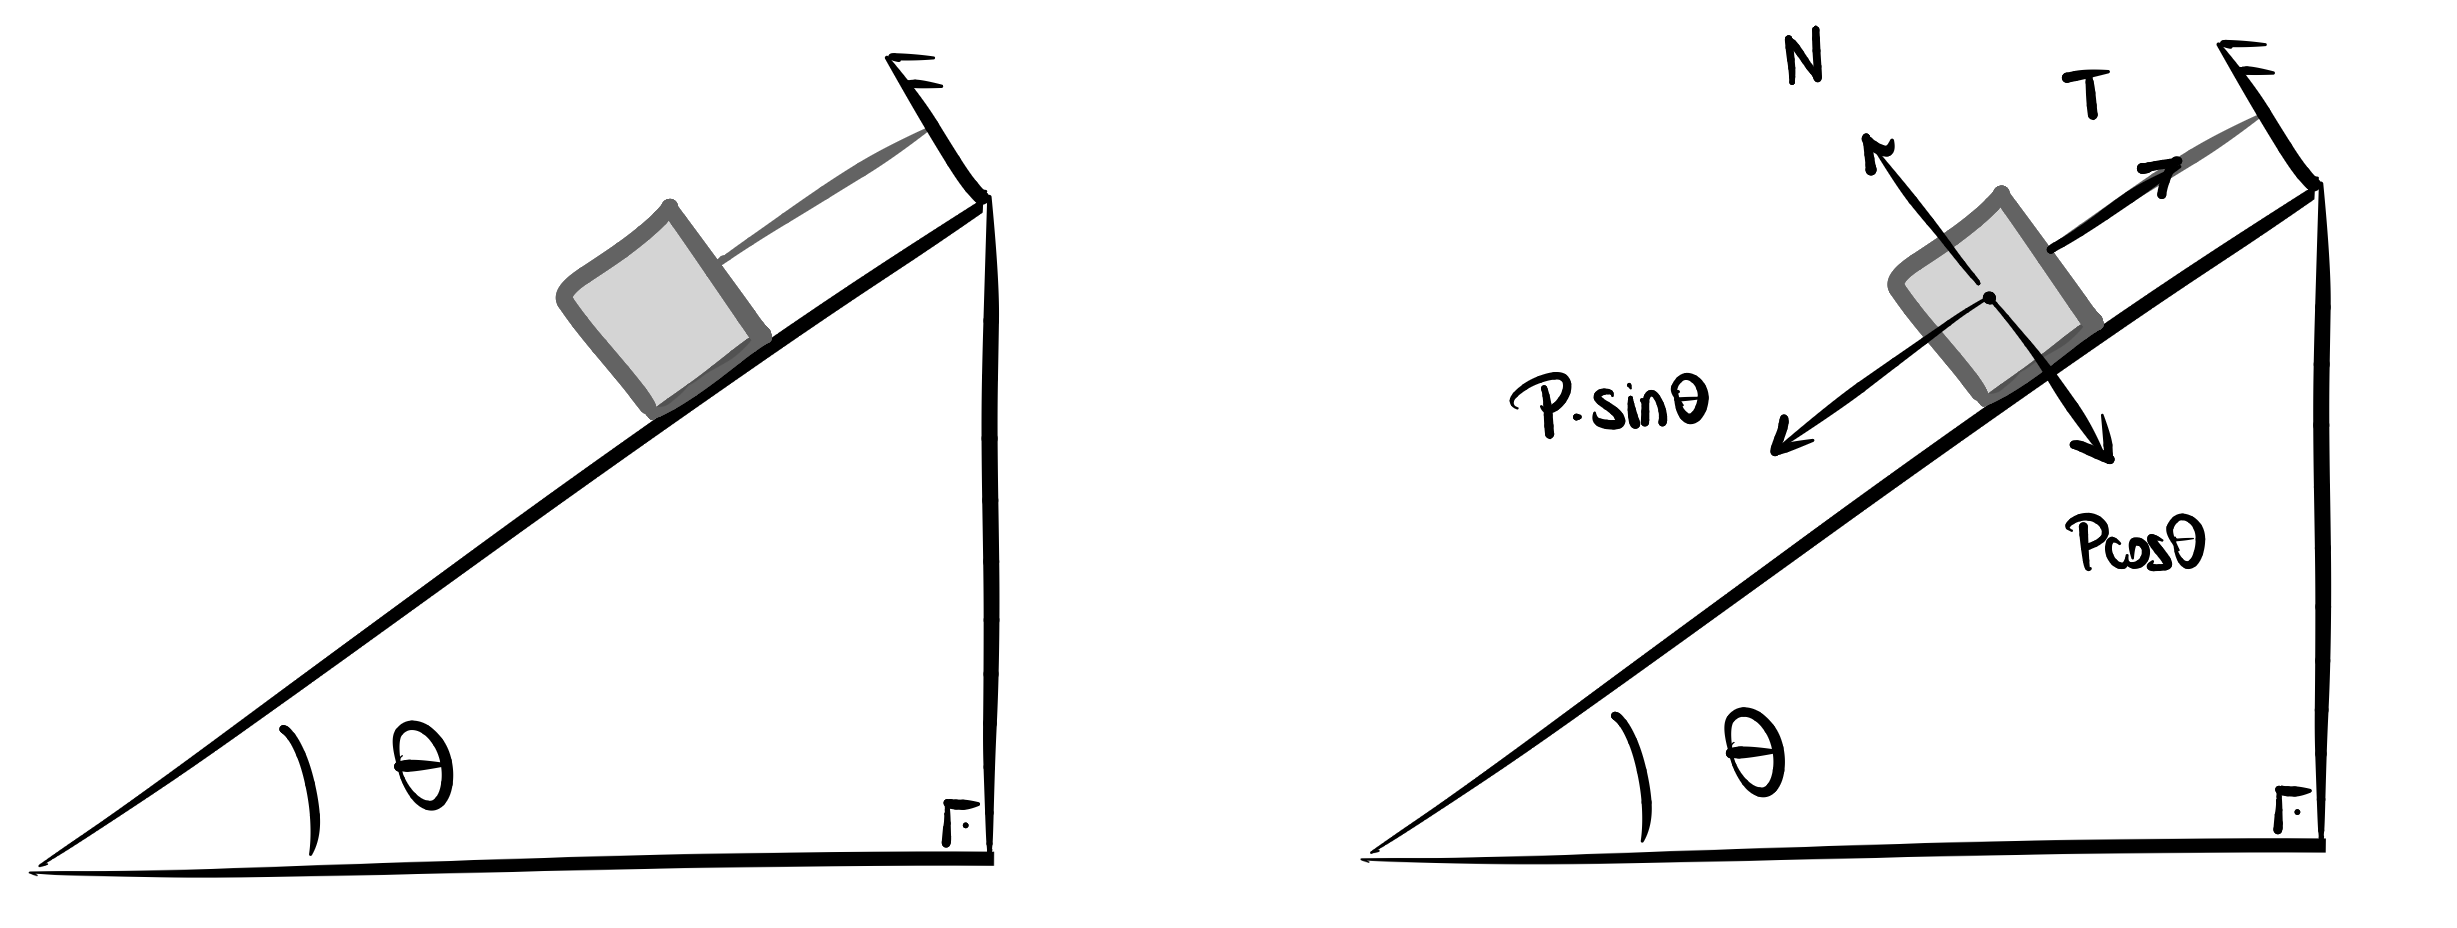
\includegraphics[width=0.6\linewidth]{imagensdinamicanewton/planoinclinadoequilibrio.png}};
  \end{scope}
\end{tikzpicture}
\captionof{figure}{}
\label{fig_newton_planoinclinadoequilibrio}
} 
\vspace{0.3cm}

Do equilíbrio na direção normal tem-se

$$ F_{Ry} = 0 \implies \boxed{N=P\cos \theta ,}$$

\noindent enquanto que o equilíbrio na direção paralela ao plano exige que

$$ F_{Rx} = 0 \implies \boxed{T=P\sin \theta.} $$

Ora, se a máxima tração no fio é de $282$ N, o valor máximo da massa $m$ do bloco para que ele fique em equilíbrio será aquele tal que a equação acima seja satisfeita para o maior valor possível de tração que o fio pode suportar:

$$ T=P\sin \theta \implies 282 = mg \sin (45^\circ) \implies 282 = m \cdot 10 \cdot \dfrac{\sqrt 2}{2} \implies \boxed{m \approx 40 \text{ kg}.}$$


\end{exemplo}


\vspace{0.3cm}
\begin{exemplo}[Nível II]\label{exemplo_newton_equilibrio02}

Considere a situação da Figura \ref{fig_mec_exemploequilibrionivel11}, em que um bloco de massa $m=5$ kg é amarrado por dois fios ideais.

{
\centering
\begin{tikzpicture}
  \begin{scope}[blend mode=multiply]
    \node {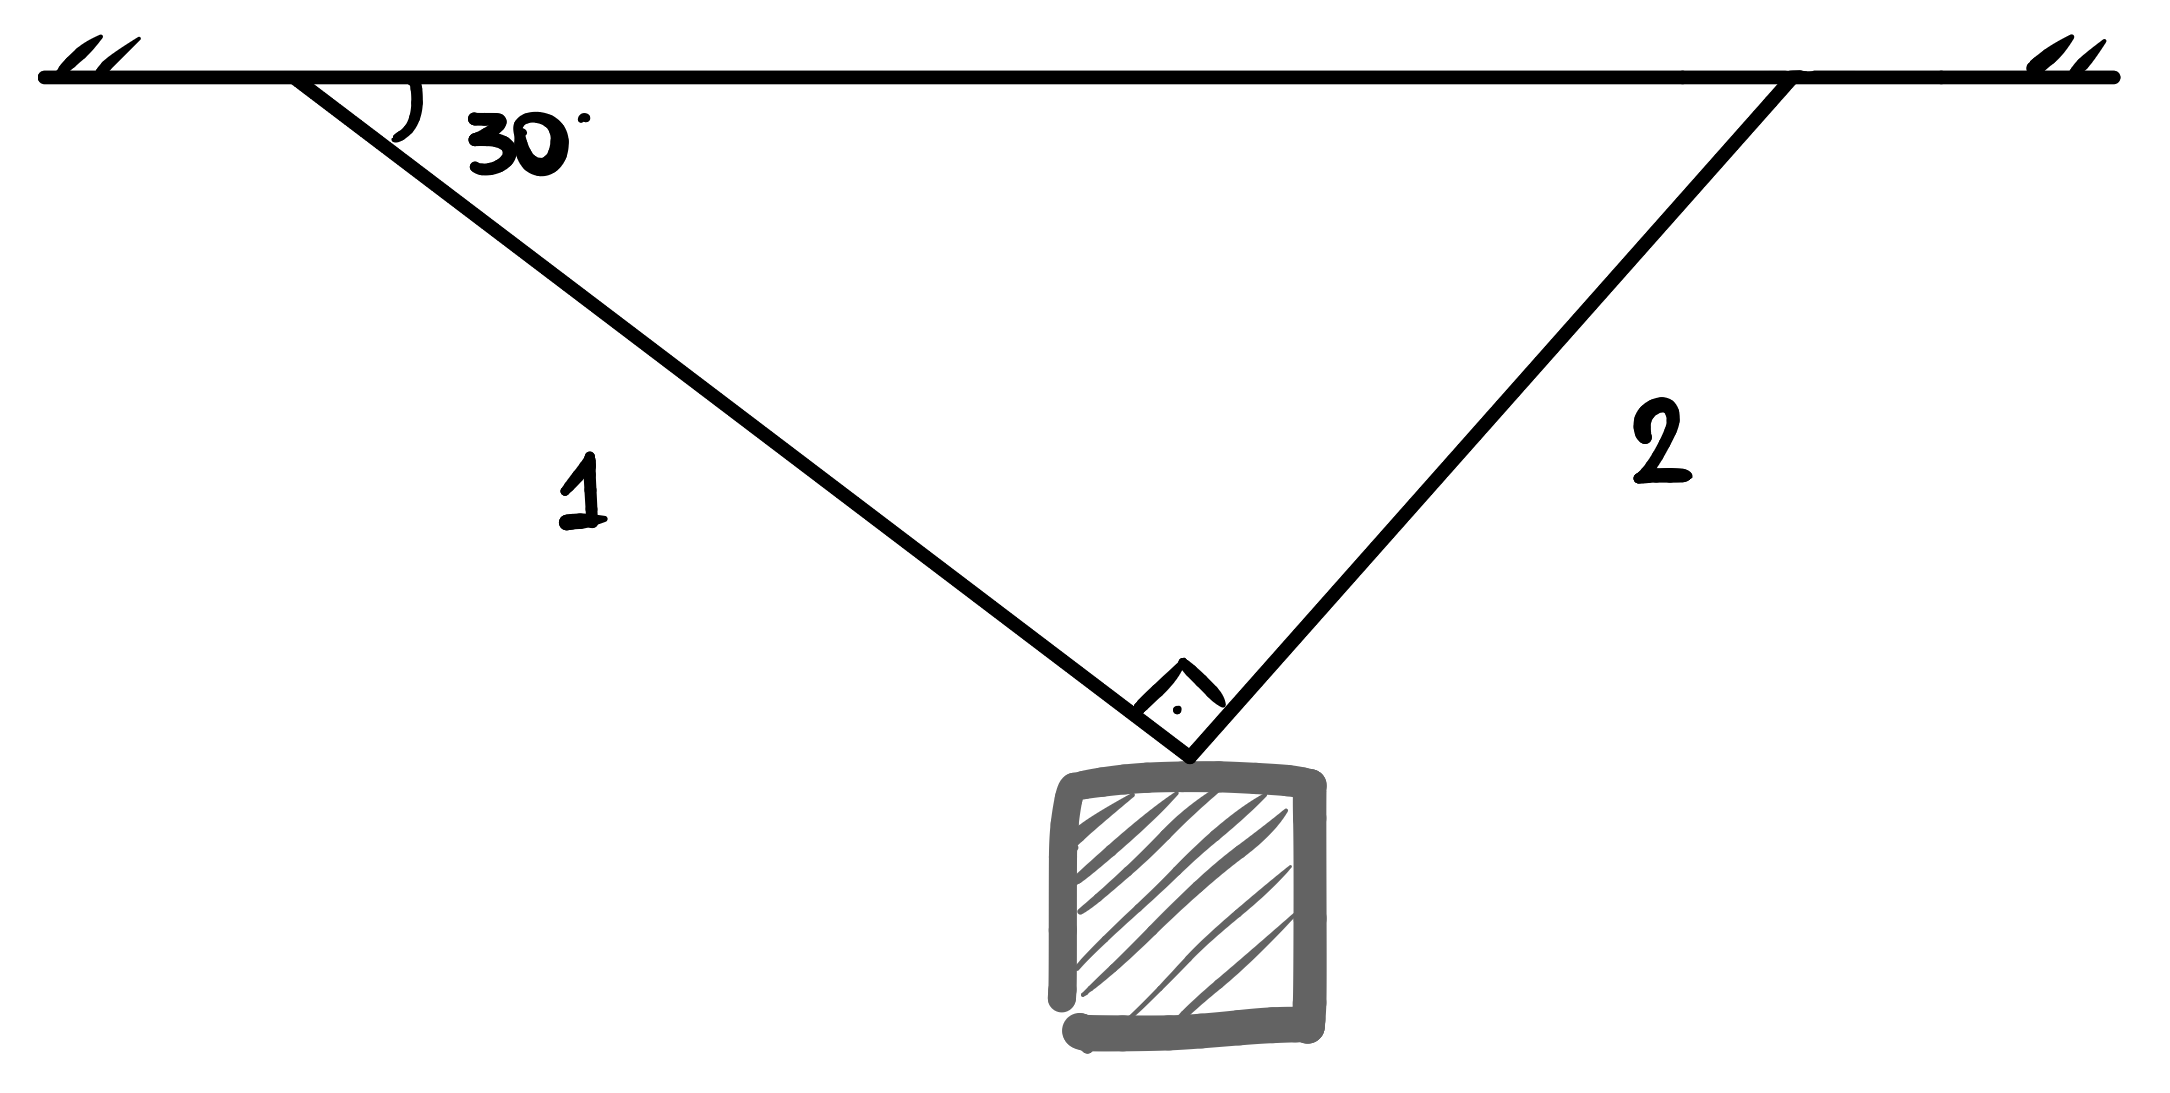
\includegraphics[width=0.4\linewidth]{imagensdinamicanewton/exemploequilibrion11.png}};
  \end{scope}
\end{tikzpicture}
\captionof{figure}{}
\label{fig_mec_exemploequilibrionivel11}
} 
\vspace{0.3cm}

Se o bloco está em equilíbrio, qual é a o valor da maior tração nos fios?

\resolucao

A figura abaixo indica o diagrama de forças que atuam na caixa. 

\vspace{0.3cm}
{
\centering
\begin{tikzpicture}
  \begin{scope}[blend mode=multiply]
    \node {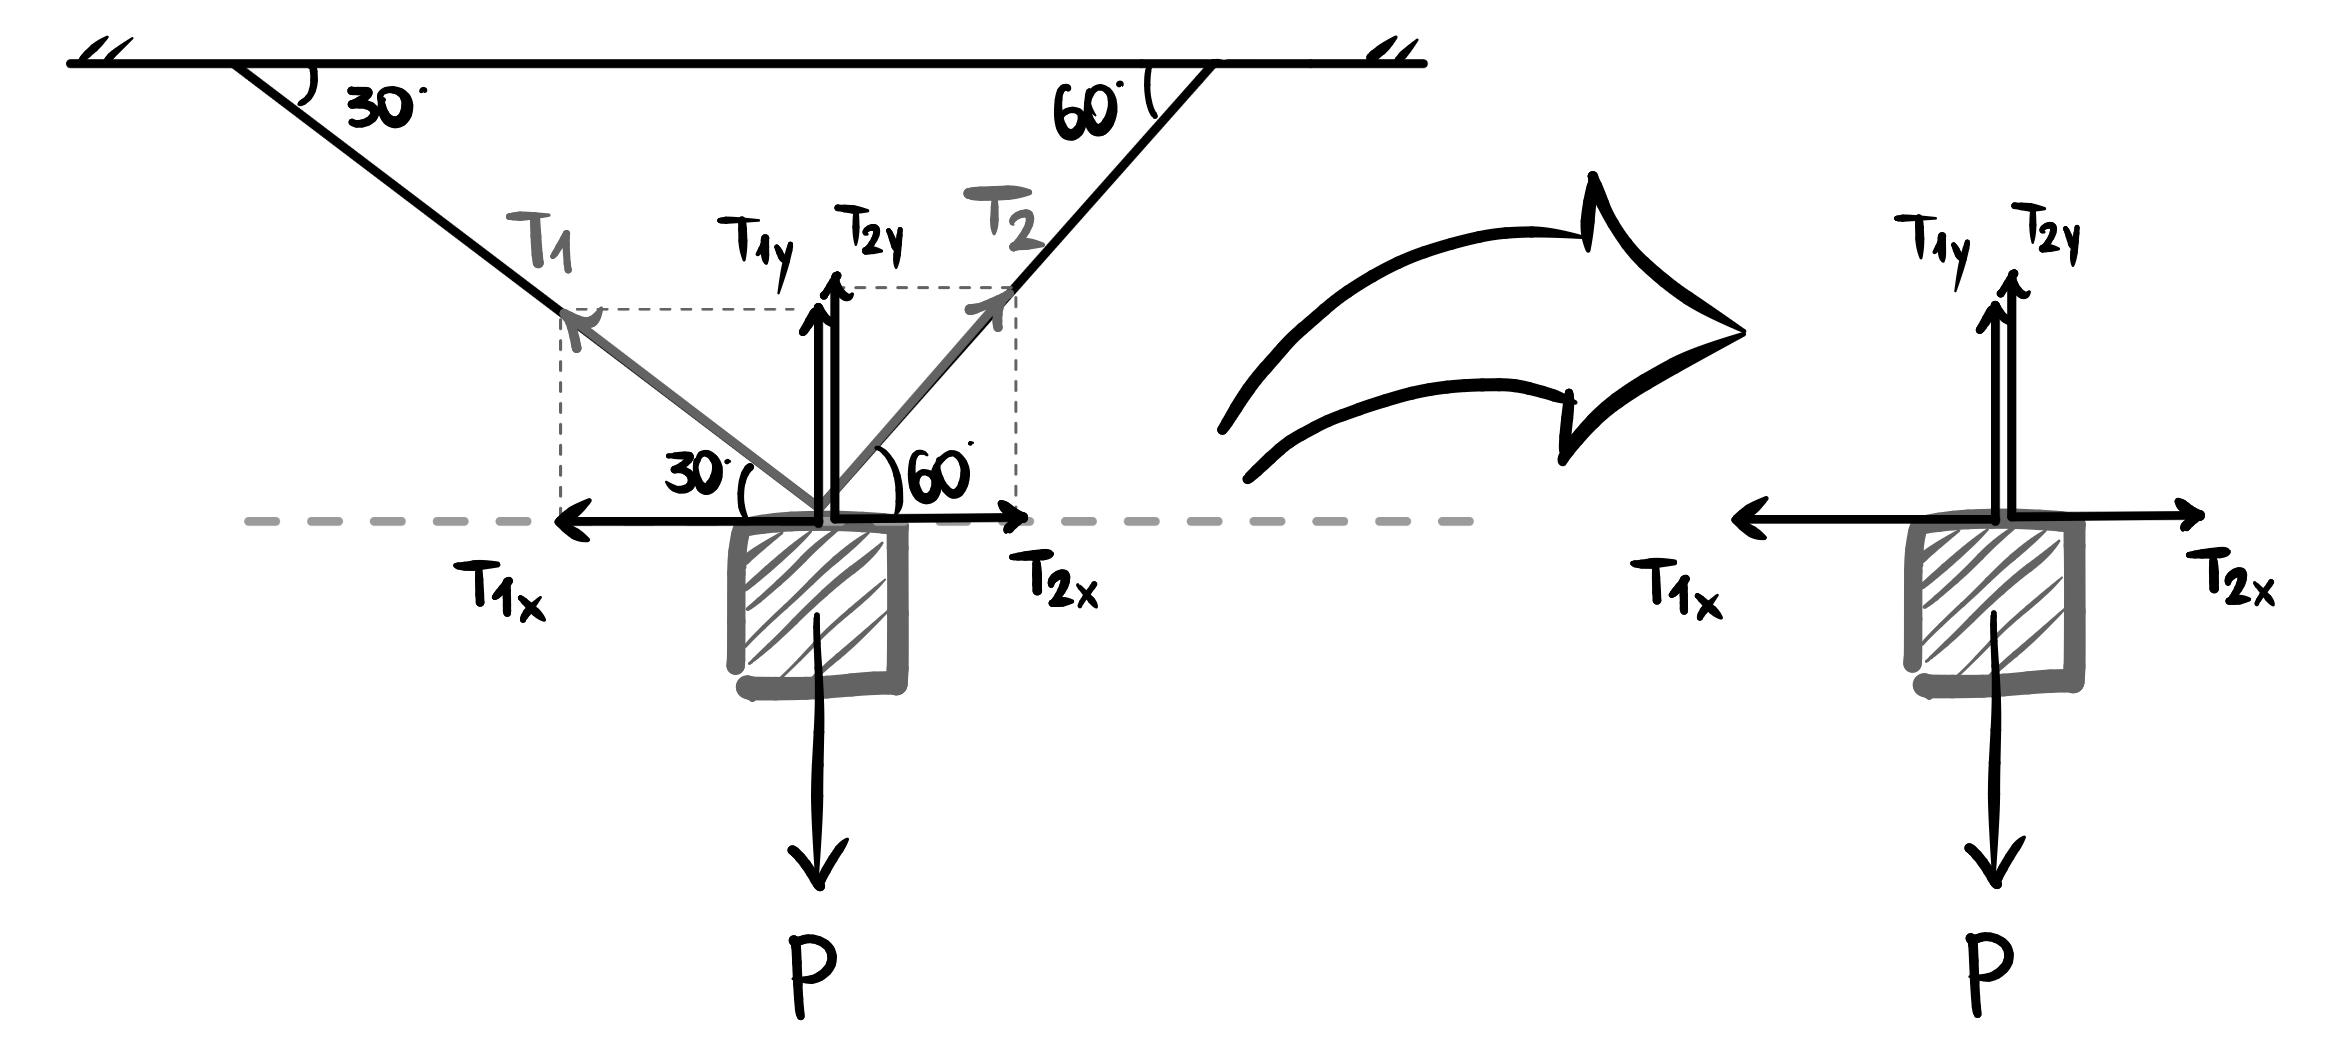
\includegraphics[width=0.7\linewidth]{imagensdinamicanewton/exemploequilibrion12.png}};
  \end{scope}
\end{tikzpicture}
\captionof{figure}{}
\label{fig_mec_exemploequilibrionivel12}
} 
\vspace{0.3cm}

O passo a passo para resolver problemas desse tipo sempre será



\begin{enumerate}
    \item Identificar o corpo cuja dinâmica queremos estudar. No caso, é a caixa.

    \item Desenhar todas as forças que atuam no corpo. Neste caso, trata-se do seu peso, que atua verticalmente para baixo e vale $P=50$N. Além das trações $T_1$ e $T_2$ que atuam nos fios $1$ e $2$, e estão na mesma direção dos fios.

    \item Como queremos impor que $F_R=0,$ daqui em diante podemos agir de duas formas diferentes. A primeira seria escolher um par de eixos perpendiculares nos quais iríamos decompor todas as forças, obrigando-as a serem nulas nas duas direções. 

    Neste caso, escolhemos as direções vertical e horizontal, e, por meio da decomposição vetorial, temos, para o fio 1:

    $$ T_{1x} = T_1 \cos (30) \implies \boxed{T_{1x}=\dfrac{T_1 \sqrt{3}}{2}} \quad \text{e} \quad  T_{1y} = T_1 \sin (30) \implies \boxed{T_{1y}=\dfrac{T_1} {2}.}  $$

    Já para o fio 2 teríamos

     $$ T_{2x} = T_2 \cos (60) \implies \boxed{T_{2x}=\dfrac{T_2}{2}} \quad \text{e} \quad  T_{2y} = T_2 \sin (60) \implies \boxed{T_{2y}=\dfrac{T_2 \sqrt3} {2}.}  $$

     Feito isso, impomos a condição de equilíbrio nas duas direções, isto é, para a direção horizontal teríamos

     $$ F_{Rx} = 0 \implies T_{1x} = T_{2x} \implies  \dfrac{T_1 \sqrt{3}}{2} = \dfrac{T_2}{2} \implies \boxed{T_2=T_1\sqrt 3,}$$

     \noindent e, para a direção vertical, teríamos

     $$ P = T_{1y}+T_{2y} \implies 50 = \dfrac{T_1}{2} + \dfrac{T_2 \sqrt 3}{2} \implies \boxed{T_1 + T_2 \sqrt 3 = 100.}$$

     Usando que $T_2=T_1 \sqrt 3$ na equação acima, somos levados a 

     $$T_1 + (T_1 \sqrt3) \sqrt 3 = 100 \implies T_1 = 25\text{N},$$

     \noindent de modo que a tração no fio 2 é $T_2=T_1 \sqrt 3= 25\sqrt3 \text{N}.$ Logo, a maior tração ocorre no fio 2, e vale $T_2 = 25\sqrt3 \text{N}.$

     
\end{enumerate}

Poderíamos ter procedido de um modo diferente no terceiro passo. Este caminho costuma parecer um pouco mais abstrato no começo, porque exige um maior manejo geométrico. Mas, como veremos, os cálculos se tornarão bem mais simples. \\

Neste caso, ao invés de decompor as forças para falar que elas se anulam em $x$ e em $y$, escreveremos uma única equação vetorial de equilíbrio: 


\[
 \vec{F}_R = 0
\quad \xrightarrow{\text{projeção nos eixos}}
\quad
\begin{cases}
F_x = 0 \\
F_y = 0
\end{cases}
\]

Ou seja, ao invés de projetarmos nos eixos e escrevermos duas equações de equilíbrio, escreveremos uma única equação, porém elas será vetorial -- e, por isso, exigirá uma interpretação geométrica. Impondo que $\vec{F}_R=0,$ teremos

$$\vec{T}_1+\vec{T}_2+\vec{P}=0.$$

É importante que o leitor perceba que a equação acima é vetorial: ela leva em consideração o vetor $\vec{T_1},$ com sua direção e sentido. Enquanto que a equação que envolve $T_{1x}$ não é vetorial, mas escalar: ela envolve o valor de uma projeção do vetor $\vec T_1$ -- o tamanho da sua projeção horizontal.

Tal equação pode ser reescrita como 

$$\vec{T}_1+\vec{T}_2+\vec{P}=0 \implies \vec{T}_1+\vec{T}_2 = -\vec{P} ,$$

\noindent ou seja, os vetores $\vec T_1 \text{ e } \vec T_2$ somados devem resultar no oposto do vetor peso. A Figura \ref{fig_mec_exemploequilibrioexemplofios} ilustra essa situação. 


\vspace{0.3cm}
{
\centering
\begin{tikzpicture}
  \begin{scope}[blend mode=multiply]
    \node {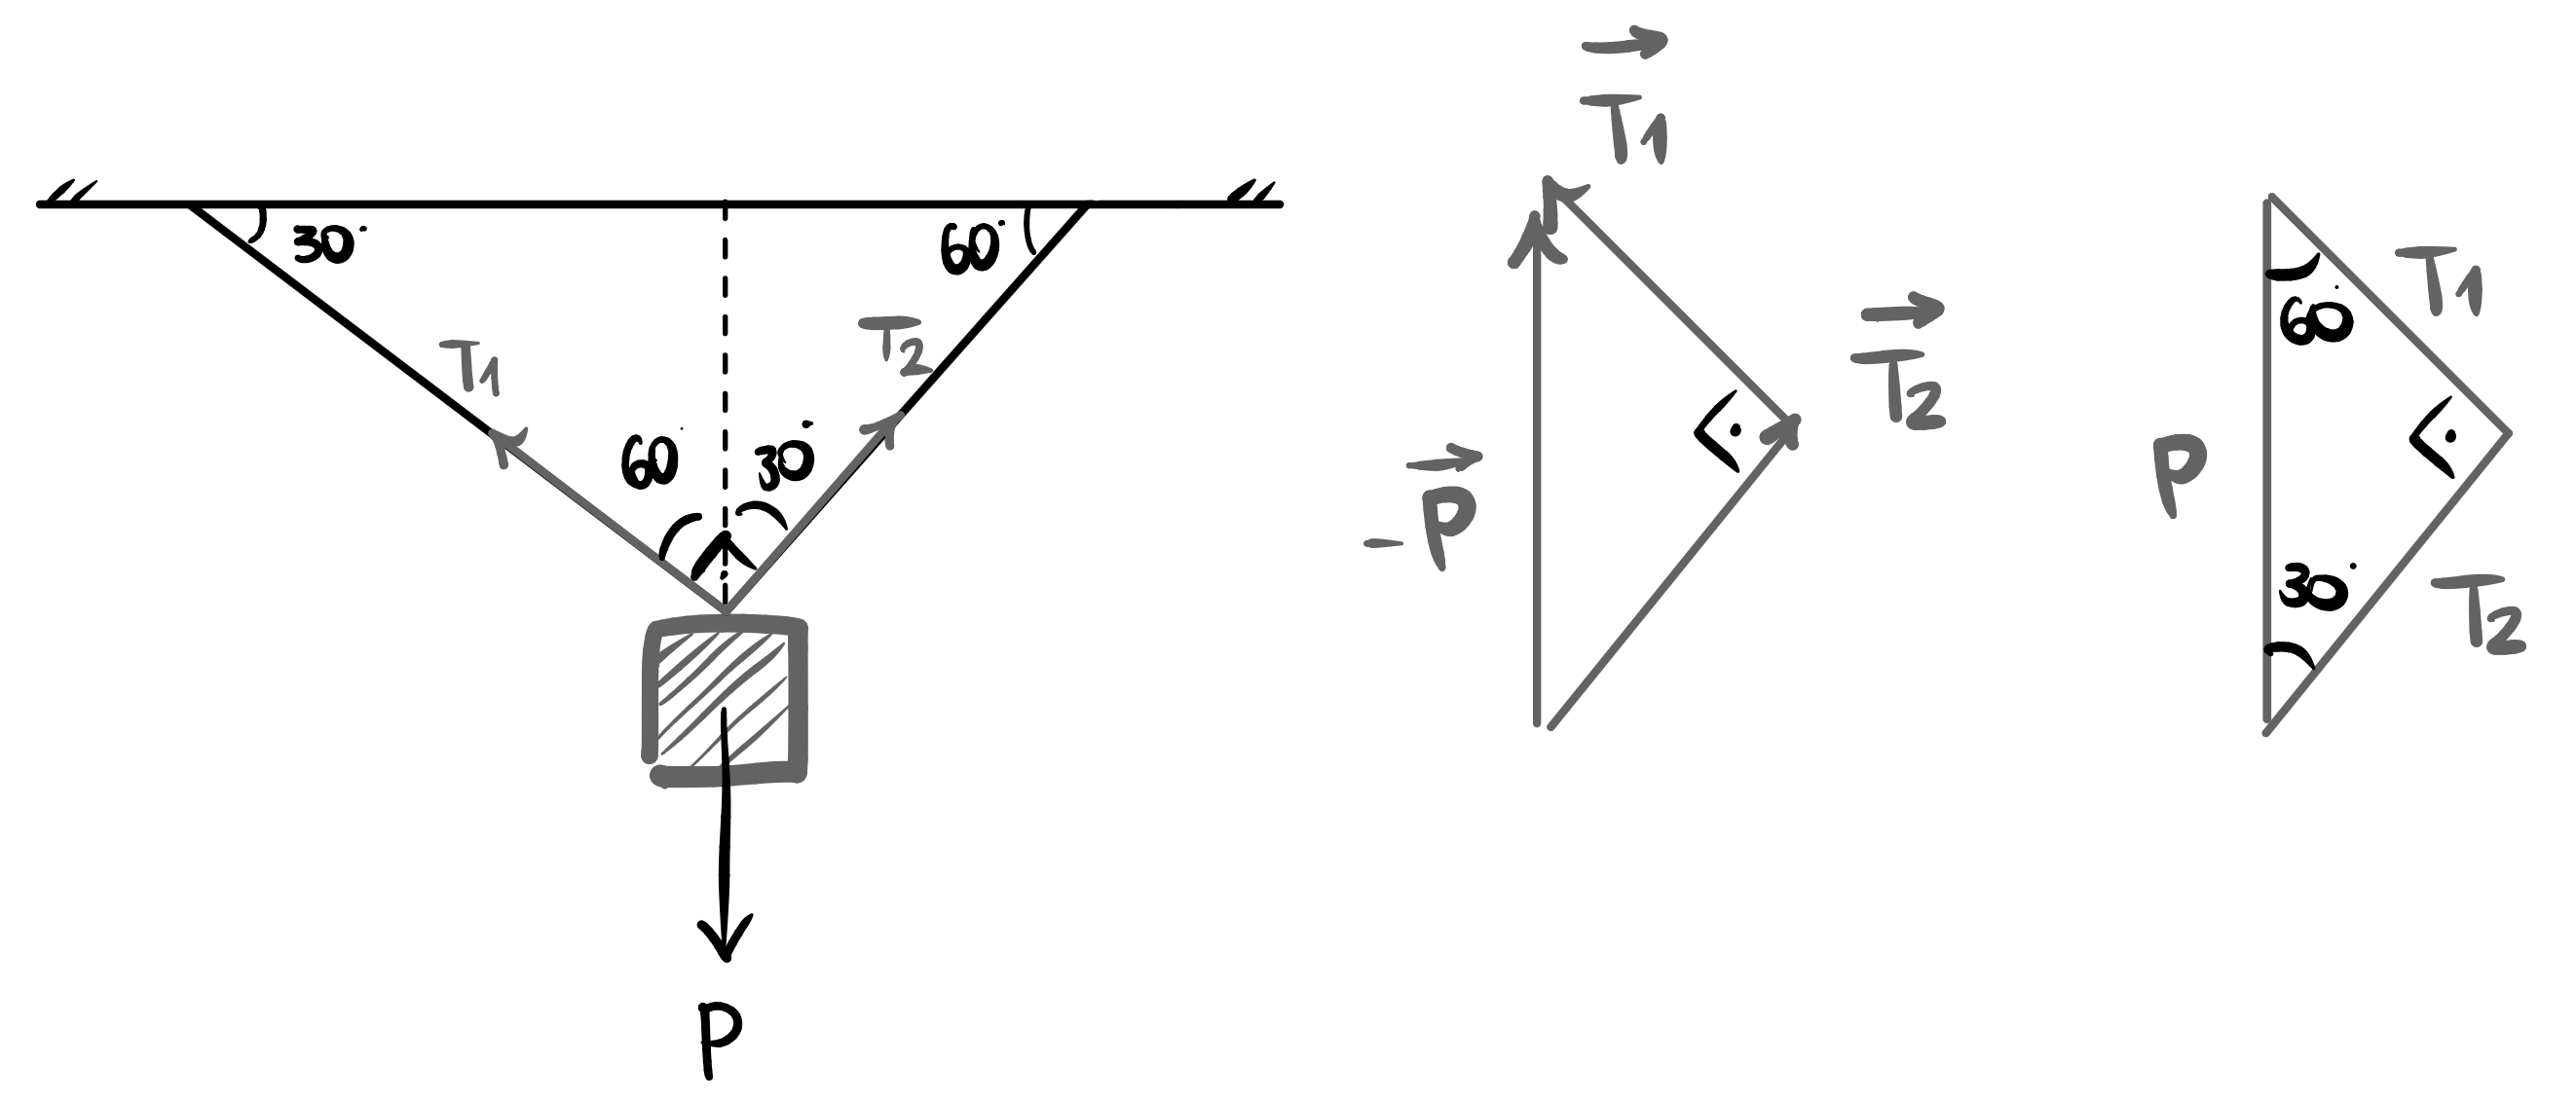
\includegraphics[width=0.7\linewidth]{imagensdinamicanewton/equilibrio exemplo fios.png}};
  \end{scope}
\end{tikzpicture}
\captionof{figure}{}
\label{fig_mec_exemploequilibrioexemplofios}
} 
\vspace{0.3cm}



Como vemos, na primeira imagem, optamos por não decompor os vetores. A imagem do meio mostra, geometricamente, o que significa a equação vetorial $ \vec{T}_1+\vec{T}_2 = -\vec{P},$ enquanto que a última imagem desconsidera o seu caráter vetorial (para onde as setas apontam) e mantém apenas suas características geométricas: tem-se um triângulo, retângulo (haja vista que os fios eram perpendiculares) de lados cujos tamanhos medem $P,$ $T_1$ e $T_2.$ \\

A primeira imagem da figura já indica que o ângulo entre o fio 1 e a vertical (direção do peso) é igual a $60^\circ$, enquanto que o ângulo entre o fio 2 e a vertical (direção do peso) é de $30^\circ$. Tais informações estão no triângulo da última figura, nos ângulos entre as direções de $T_1$ e $T_2$ com a vertical (direção do peso). \\

Note que, até então, ainda não fizemos nenhum cálculo, apenas uma construção geométrica. Munidos dela, podemos obter as trações diretamente, com um único cálculo, usando a definição das razões trigonométricas no triângulo retângulo. Para o caso de $T_2,$ teríamos

$$ \sin(60^\circ) = \dfrac{T_2}{P} \implies T_2 = P \sin(60^\circ) = 50 \cdot \dfrac{\sqrt 3}{2} \implies \boxed{T_2 =25 \sqrt 3 \text{N}.} $$

Perceba que este segundo caminho torna o cálculo algébrico muito simples, por trocar duas equações (equilíbrio em $x$ e em $y)$ por uma única. O preço a se pagar é que a equação de equilíbrio vetorial precisa ser interpretada geometricamente. Isso, contudo, sempre vai ocorrer: se um corpo está em equilíbrio sobre a ação de um certo número de forças, então tais forças irão formar um polígono fechado. No caso de 3 forças, trata-se de um triângulo. Se fossem 4 ou 6 teríamos um quadrilátero e um hexágono, respectivamente. Tais figuras nos permitirão escrever, geometricamente, a equação de equilíbrio $\vec F_R =0.$



\end{exemplo}



\vspace{0.3cm}



\begin{exemplo}[Nível III]\label{exemplo_newton_equilibrio03}

Considere a generalização do exemplo anterior: um bloco de massa $m$ está preso por dois fios, que fazem os ângulos $\theta$ e $\phi$ com a parede do teto, como mostra a Figura \ref{fig_mec_leisnewtonequilibrioexemplonivel31}.


\vspace{0.3cm}
{
\centering
\begin{tikzpicture}
  \begin{scope}[blend mode=multiply]
    \node {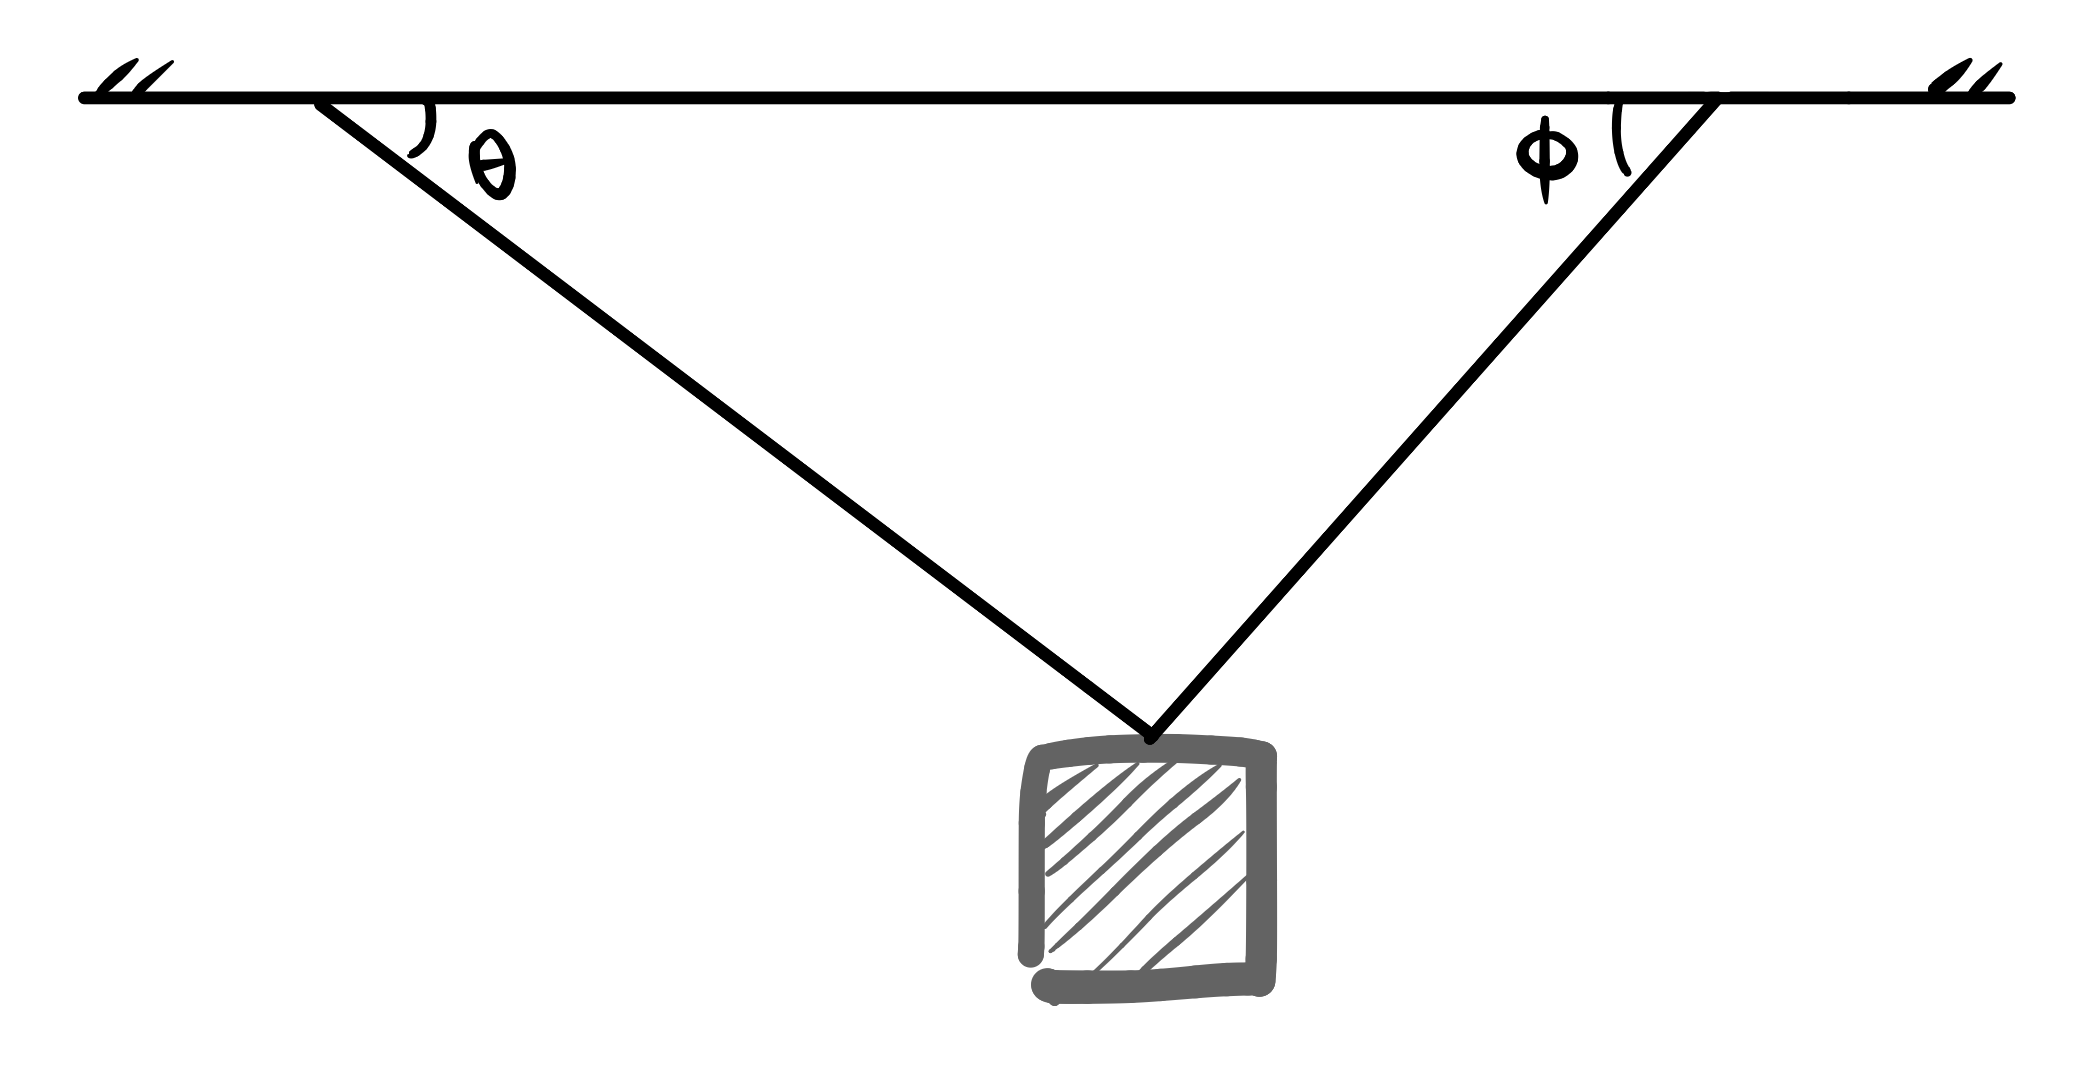
\includegraphics[width=0.4\linewidth]{imagensdinamicanewton/leisnewtonequilibrioexemplonivel31.png}};
  \end{scope}
\end{tikzpicture}
\captionof{figure}{}
\label{fig_mec_leisnewtonequilibrioexemplonivel31}
} 
\vspace{0.3cm}


Encontre a razão entre as trações nos fios quando o bloco está em repouso.

\resolucao

A Figura \ref{fig_mec_leisnewtonequilibrioexemplonivel32} ilustra o diagrama de forças na caixa. Tomando o segundo caminho do exemplo anterior, escreveremos uma única equação de equilíbrio, a equação vetorial:

$$ \vec F_R = \vec T_1 + \vec T_2 + \vec P = 0 \implies \vec T_1 + \vec T_2 = - \vec P.$$

Ou seja, os vetores $\vec T_1 $ e $\vec T_2 $ somados devem dar um vetor vertical, apontando para cima, do mesmo tamanho do vetor peso. Tal situação está representada no triângulo no desenho da direita da Figura \ref{fig_mec_leisnewtonequilibrioexemplonivel32}.

\vspace{0.3cm}
{
\centering
\begin{tikzpicture}
  \begin{scope}[blend mode=multiply]
    \node {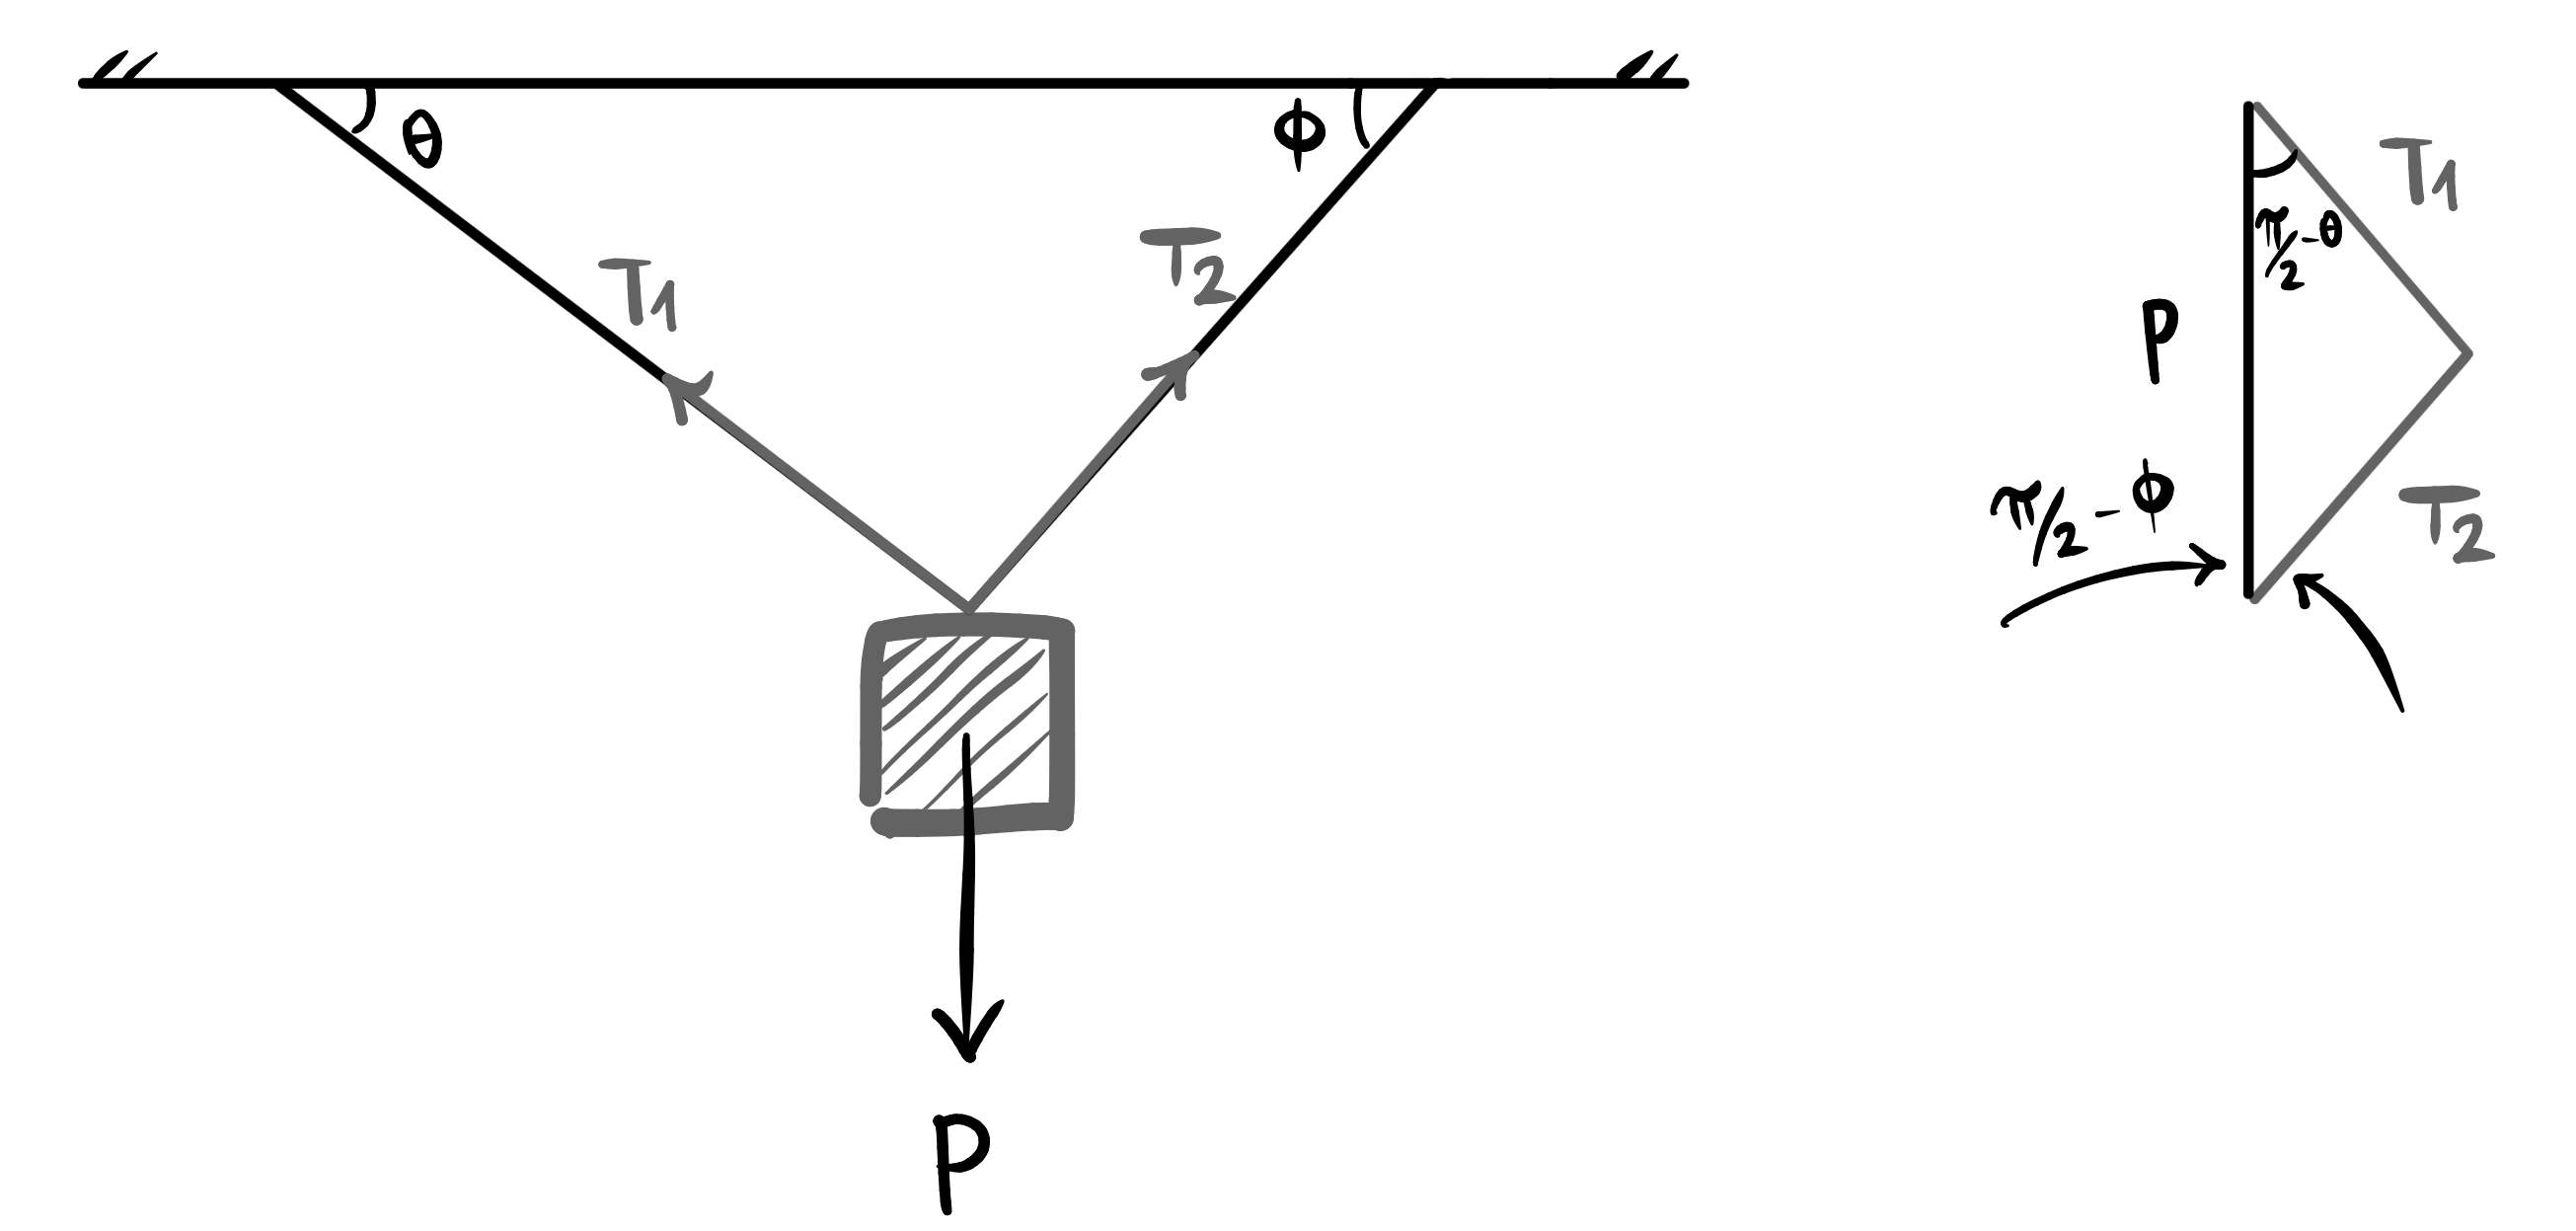
\includegraphics[width=0.7\linewidth]{imagensdinamicanewton/leisnewtonequilibrioexemplonivel32.png}};
  \end{scope}
\end{tikzpicture}
\captionof{figure}{}
\label{fig_mec_leisnewtonequilibrioexemplonivel32}
} 
\vspace{0.3cm}

Da imagem da esquerda de tal figura, ao traçar uma vertical passando pelo centro da caixa, obtém-se facilmente os ângulos entre os fios e a vertical, que aparecem representados já no triângulo da figura da direita. Pela Lei dos Senos em tal triângulo podemos escrever que

$$ \dfrac{T_2}{\sin \left( \dfrac{\pi}{2} - \theta \right)} = \dfrac{T_1}{\sin \left( \dfrac{\pi}{2} - \phi \right)} = \dfrac{P}{\sin \left(\phi +\theta \right)}.$$

Da primeira igualdade extraímos

$$ \boxed{\dfrac{T_2}{T_1} = \dfrac{\cos \theta}{\cos \phi}.}$$



\end{exemplo}









\begin{secnivel}[Força na Polia Fixa]{I}{Força na Polia Fixa}
  
  \eqLdois{dem}{eq_newton_poliafixa}{F_\text{FINAL}=F}

\end{secnivel}


 A força $F$ em tal equação representa a força feita por um indivíduo na extremidade uma corda que passa por uma polia (roldana) fixa, como mostra Figura \ref{fig_dinamicanewton_poliafixa01}. A força $F_\text{FINAL}$ que chega em uma extremidade da corda é igual à força $F$ feita na outra extremidade.

A Equação \eqref{eq_newton_poliafixa}, portanto, constata que a força transmitida ao longo do fio é a mesma.




\secgfe{De onde vem}

Uma polia -- ou roldana -- fixa é aquela que está, como o próprio nome indica, presa em alguma parede ou anteparo. Sendo assim, ela está fixa e não tem nenhuma liberdade de se mover. Em polias fixas ideais\footnote{Sempre trabalharemos com polias ideias -- aquelas de massa desprezível -- no contexto do Ensino Médio. Do contrário, sua inércia de rotação teria que ser levada em conta, o que exigiria cálculos mais avançados do que as ferramentas do ensino médio possibilitam fazer.} o seu uso será apenas o de mudar a direção em que se aplica a força, como mostra a Figura \ref{fig_dinamicanewton_poliafixa01}.

Perceba, em tal figura, que para sustentar parado, digamos, um bloco de peso $P=200$N, a força necessária a ser feita deverá ser exatamente igual a $200$N. O indivíduo pode puxar a corda em diferentes direções, mas sempre terá que fazer uma força exatamente igual ao peso do bloco para mantê-lo parado. A roldana fixa, portanto, é um dispositivo que não aumenta o diminui a força feita em uma extremidade -- a força se transmite integralmente até a outra extremidade do fio.

A utilidade de um dispositivo como esse, portanto, não é puxar um bloco fazendo menos força do que o valor de seu peso, mas apenas o de facilitar a execução de tal força por fazê-la através de uma corda.

\vspace{0.3cm}
{
\centering
\begin{tikzpicture}
  \begin{scope}[blend mode=multiply]
    \node {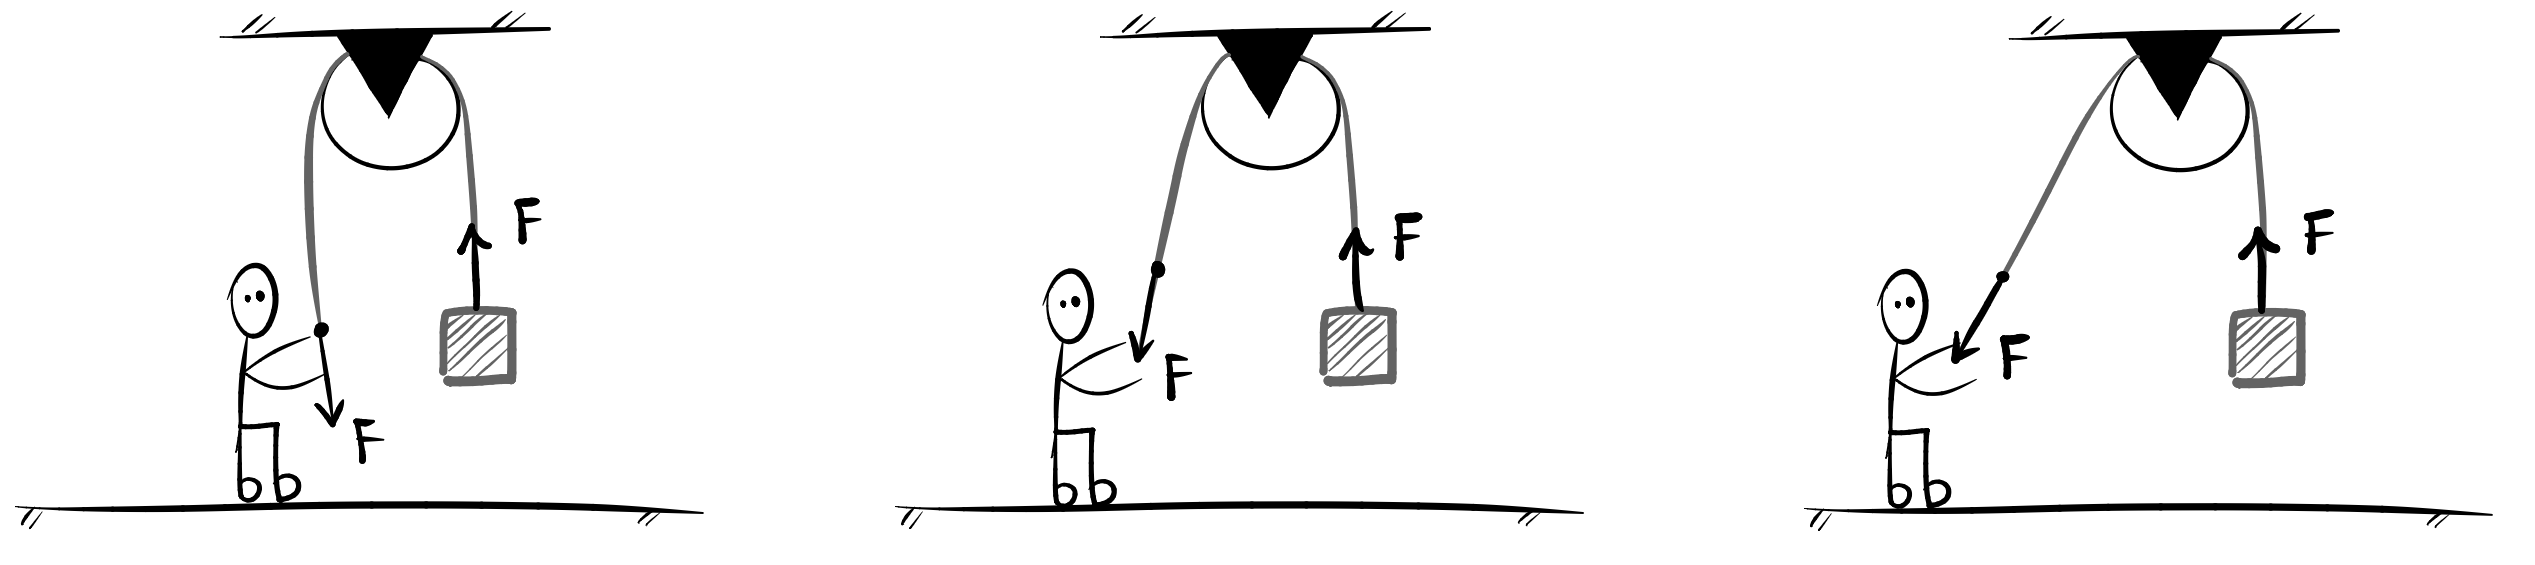
\includegraphics[width=0.9\linewidth]{imagensdinamicanewton/poliafixa01.png}};
  \end{scope}
\end{tikzpicture}
\captionof{figure}{O funcionamento de uma polia fixa.}
\label{fig_dinamicanewton_poliafixa01}
} 
\vspace{0.3cm}

No desenvolvimento da Equação \eqref{eq_newton_terceiraleinewton} nós exploramos o conceito de tração em um fio e a definição de um fio ideal. Ali nós provamos, matematicamente, que ao longo de um fio ideal a tração é sempre a mesma. Como o sistema de uma roldana fixa consiste em um disco fixado e um fio ideal que passa através dele, é de se esperar que a força (tração) ao longo do fio seja sempre a mesma, como provamos na discussão sobre a Terceira Lei de Newton. É exatamente isso que a Equação \eqref{eq_newton_poliafixa} diz.

\secgfe{Onde é usada}

Polias aparecem em diversos contextos nos quais deseja-se, em geral, carregar um objeto pesado. Diversos aparelhos de academias possuem polias, para mudar a direção com que se aplica certas forças ao carregar um mesmo peso, a fim de trabalhar músculos diferentes, por exemplo.

Imagine a dificuldade em carregar um objeto grande e pesado, como, digamos, um piano. É muito mais fácil amarrá-lo por uma corda e puxá-lo por essa corda, em um sistema como o da Figura \ref{fig_dinamicanewton_poliafixa01}. Por mais que a força exercida na corda deva ser pelo menos igual ao peso do piano para levantá-lo, será muito mais simples executar tal força ao longo de uma corda -- o que pode inclusive ser realizado por uma máquina, como no funcionamento de um elevador -- do que carregar o piano diretamente. 

\secgfe{Erros comuns}

Os erros mais comuns aqui consistem em confundir a polia fixa com a polia móvel, que será estudada na próxima seção. 

Além disso é comum o estudante acreditar que a força necessária para carregar um objeto na situação da Figura \ref{eq_newton_poliafixa} irá depender do ângulo da corda. Tal figura, contudo, já mostra que isso está equivocado: a força que se propaga no fio é sempre a mesma feita na outra extremidade, independente da direção do fio.


\secgfe{Observações}

Costuma-se dizer que a polia fixa é um sistema que não oferece vantagem mecânica, isto é, a força que se faz é exatamente a mesma que chega na outra extremidade. Um dispositivo que oferece vantagem mecânica seria aquele que multiplica essa força ao longo do seu caminho, como a própria polia móvel o faz, como veremos.

Contudo, embora a polia fixa não reduza a intensidade da força necessária para erguer um corpo -- já que, no modelo ideal, a tração no fio é igual ao peso da carga -- ela pode tornar o esforço humano significativamente mais confortável e eficiente do ponto de vista biomecânico. Ao permitir que a pessoa puxe o fio para baixo em vez de levantar o peso para cima, a polia transforma a ação em algo mais natural: é mais fácil aplicar força no sentido descendente, aproveitando o próprio peso do corpo e recrutando grupos musculares mais fortes, como os dorsais e os bíceps, em vez de depender apenas dos ombros. Além disso, puxar para baixo melhora o equilíbrio e o controle do movimento, reduzindo a instabilidade. 

Assim, a polia fixa não oferece vantagem mecânica em termos físicos -- não há redução da força exigida --, mas oferece uma vantagem operacional e ergonômica que explica por que ela é tão útil na prática e porque, mesmo fazendo a mesma força, o esforço necessário para carregar o mesmo objeto pareça menor usando um sistema de polia fixa.


\vspace{0.3cm}


\begin{exemplo}[Nível I]\label{exemplo_newton_poliafixa01}

Considere a situação da Figura \ref{fig_mec_poliafixaex1} em que o ângulo do plano inclinado é $\theta = 30^\circ$ e a massa do bloco é $m=10$ kg. Se o bloco sobe com velocidade constante, qual é a força feita pelo menino?

{
\centering
\begin{tikzpicture}
  \begin{scope}[blend mode=multiply]
    \node {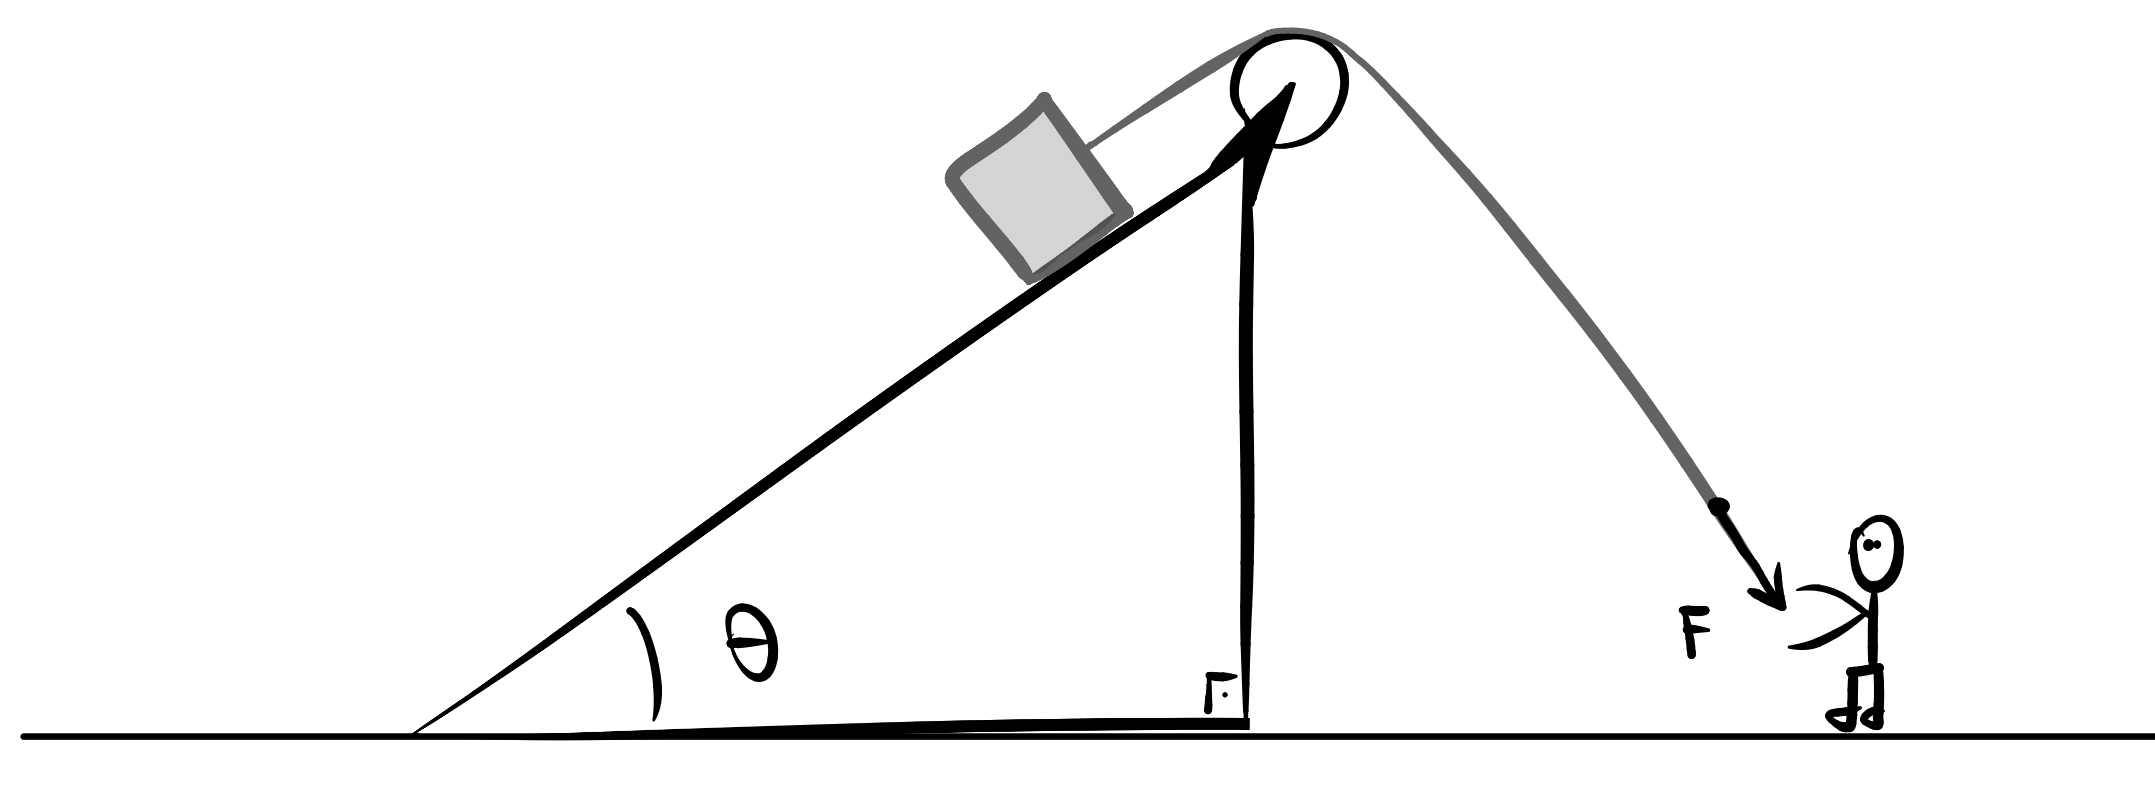
\includegraphics[width=0.5\linewidth]{imagensdinamicanewton/poliafixa1.png}};
  \end{scope}
\end{tikzpicture}
\captionof{figure}{}
\label{fig_mec_poliafixaex1}
} 


\resolucao

Se o bloco sobe com velocidade constante (MRU) isso significa que ele está em equilíbrio dinâmico, ou seja, $F_R =0.$ Analisando as forças na direção do plano inclinado teremos a tração puxando o bloco plano acima e a componente $P \sin \theta$ do peso puxando o bloco plano abaixo (veja o desenvolvimento da Equação \eqref{eq_dinamicanewtoniana_gsintheta} em caso de surpresa com tal expressão). Sendo assim, equacionado o equilíbrio em tal direção teremos

$$ T = P \sin \theta = mg \sin 30^\circ = 10 \cdot 10 \cdot \dfrac{1}{2} \implies T = 50 \text{ N.}$$

Como trata-se de um sistema de polia fixa, a força feita pelo menino em uma extremidade do fio é exatamente aquela que se propaga e chega na outra extremidade. Logo, o menino faz uma força $F$ tal que 

$$ \boxed{F=T=50 \text{ N.}}$$



\end{exemplo}

\vspace{0.3cm}




\begin{exemplo}[Nível II (Escola Naval - 2019)]\label{exemplo_newton_poliafixa02}

Analise a figura abaixo.


{
\centering
\begin{tikzpicture}
  \begin{scope}[blend mode=multiply]
    \node {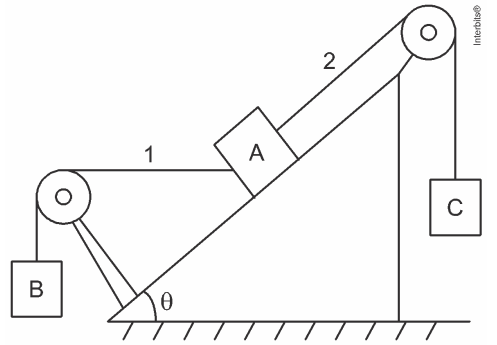
\includegraphics[width=0.4\linewidth]{imagensdinamicanewton/poliafixa2.png}};
  \end{scope}
\end{tikzpicture}
\captionof{figure}{}
\label{fig_mec_poliafixaex2}
} 


A figura representa o perfil de um plano inclinado de um ângulo $\theta$ no qual estão fixas duas polias ideais, de modo que o trecho do fio 1 é horizontal e o trecho do fio 2 é paralelo ao plano inclinado. Os fios são ideais e os atritos são desprezíveis. Sabendo-se que os blocos $A$ e $B$ têm o mesmo peso $P$, qual deve ser o peso do bloco $C$ para que o sistema permaneça em equilíbrio?

\begin{enumerate}
    \item [a)] $P(\sin\theta+\cos\theta)$
    \item [b)]$P(\sin\theta-\cos\theta)$
    \item [c)]$2P\sin\theta$
    \item [d)]$2P\cos\theta$
    \item [e)]$\dfrac{P}{2}\,(\sin\theta+\cos\theta)$
\end{enumerate}


\resolucao

A Figura \ref{fig_mec_newetonpoliafixaexmplonivel2} ilustra a situação com o diagrama de todas as forças que atuam nos blocos. Começando pela direita, a tração $T_1$ no primeiro fio deve ser igual ao peso $P_C$ do bloco $C$, isto é: $T_1 = P_C$.

\vspace{0.3cm}
{
\centering
\begin{tikzpicture}
  \begin{scope}[blend mode=multiply]
    \node {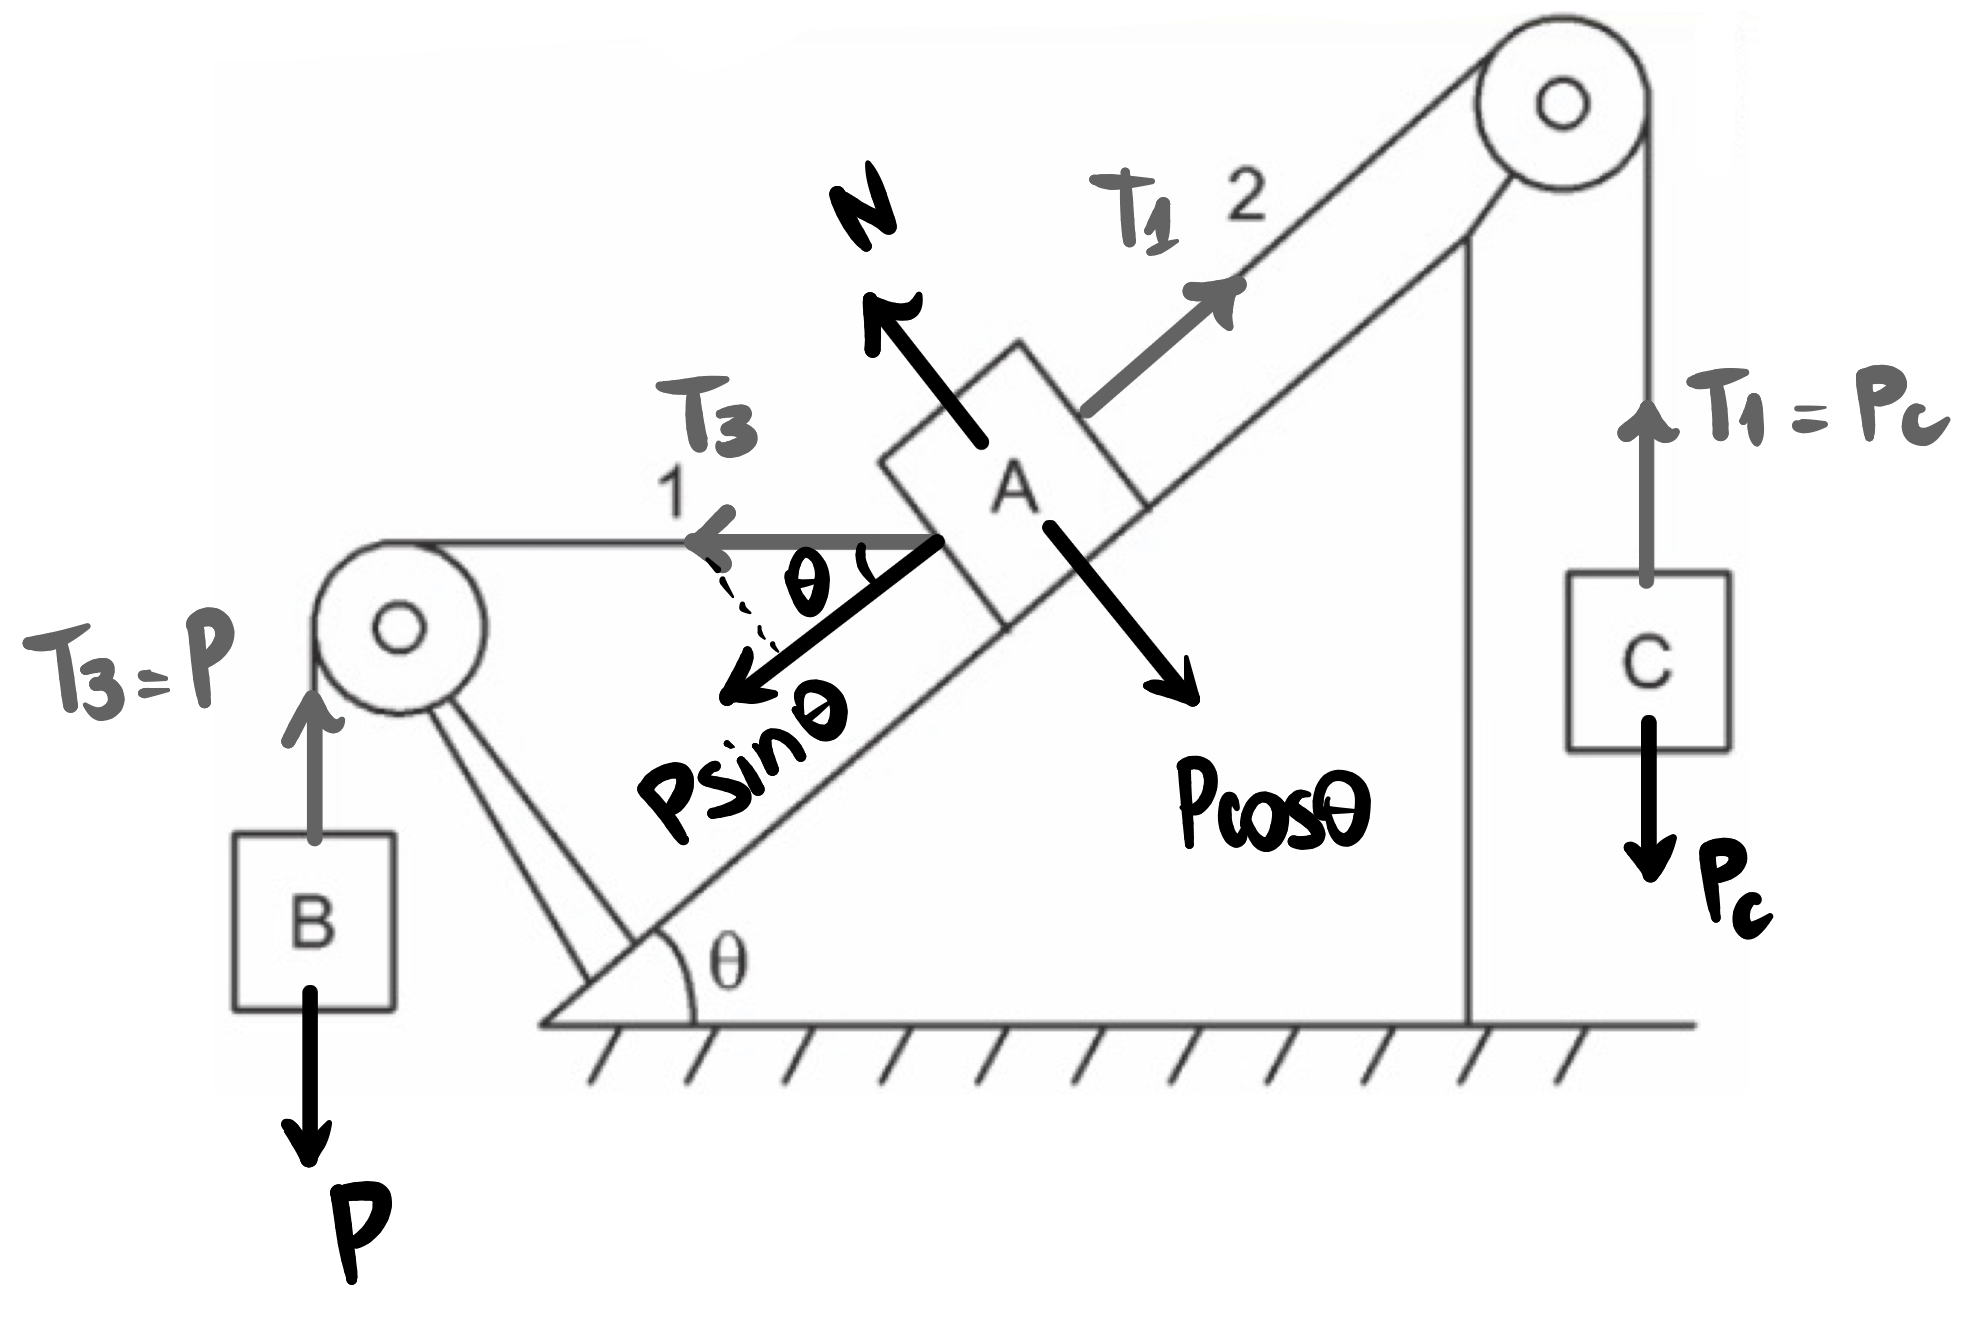
\includegraphics[width=0.45\linewidth]{imagensdinamicanewton/newetonpoliafixaexmplonivel2.png}};
  \end{scope}
\end{tikzpicture}
\captionof{figure}{}
\label{fig_mec_newetonpoliafixaexmplonivel2}
} 
\vspace{0.3cm}

Essa tração se propaga, puxando o bloco $A$ na direção plano acima. Do lado esquerdo, a tração $T_3$ no fio vertical deve ser igual ao peso $P$ do bloco $B$, ou seja, $T_3 = P.$ Essa tração se propaga, puxando horizontalmente o bloco $A.$  

Já no bloco $A$, representamos a normal $N$ feita pelo plano sob ele e a sua força peso $P$, já decomposta nas componentes paralela ao plano, $P \sin \theta$, e perpendicular ao plano, $P \cos \theta.$ Equacionando o equilíbrio das forças na direção do plano será necessário decompor a tração $T_3,$ que possui componente $T_3 \cos \theta$ na direção do plano. Logo, em tal direção, aplicando $F_\text{R} = 0,$ somos levados a

$$ P \sin \theta + T_3 \cos \theta = T_1,$$

\noindent e, como $T_3 = P$ e $T_1 = P_C$, segue que 

$$ \boxed{ P_C = P \sin \theta + P \cos \theta \implies \text{letra A}.}$$

\end{exemplo}

\vspace{0.3cm}





\begin{exemplo}[Nível III (ITA 1996)]  \label{exemplo_newton_poliamovel03}

Dois blocos de massa $M$ estão unidos por um fio de massa desprezível que passa por uma roldana com eixo fixo. 
Um terceiro bloco de massa $m$ é colocado suavemente sobre um dos blocos, como mostra a figura. 
Com que força esse pequeno bloco de massa $m$ pressionará o bloco sobre o qual foi colocado?

{
\centering
\begin{tikzpicture}
  \begin{scope}[blend mode=multiply]
    \node {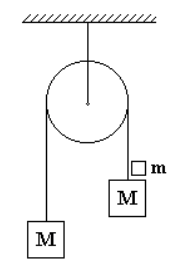
\includegraphics[width=0.2\linewidth]{imagensdinamicanewton/poliamovelexemplo03.png}};
  \end{scope}
\end{tikzpicture}
\captionof{figure}{}
\label{fig_mec_poliamovelexemplo3}
} 

\begin{enumerate}
    \item [a)] $\displaystyle \frac{2mMg}{2M + m}$
    \item [b)] $mg$
    \item [c)] $(m - M)g$
    \item [d)] $\displaystyle \frac{mg}{2M + m}$
    \item [e)] outra expressão
\end{enumerate}

\resolucao

Primeiramente, como mostra a Figura \ref{fig_mec_newtonpoliafixaexemploita}, vamos considerar o sistema dos dois blocos da direita como um único corpo de massa $(M+m).$ 

\vspace{0.3cm}
{
\centering
\begin{tikzpicture}
  \begin{scope}[blend mode=multiply]
    \node {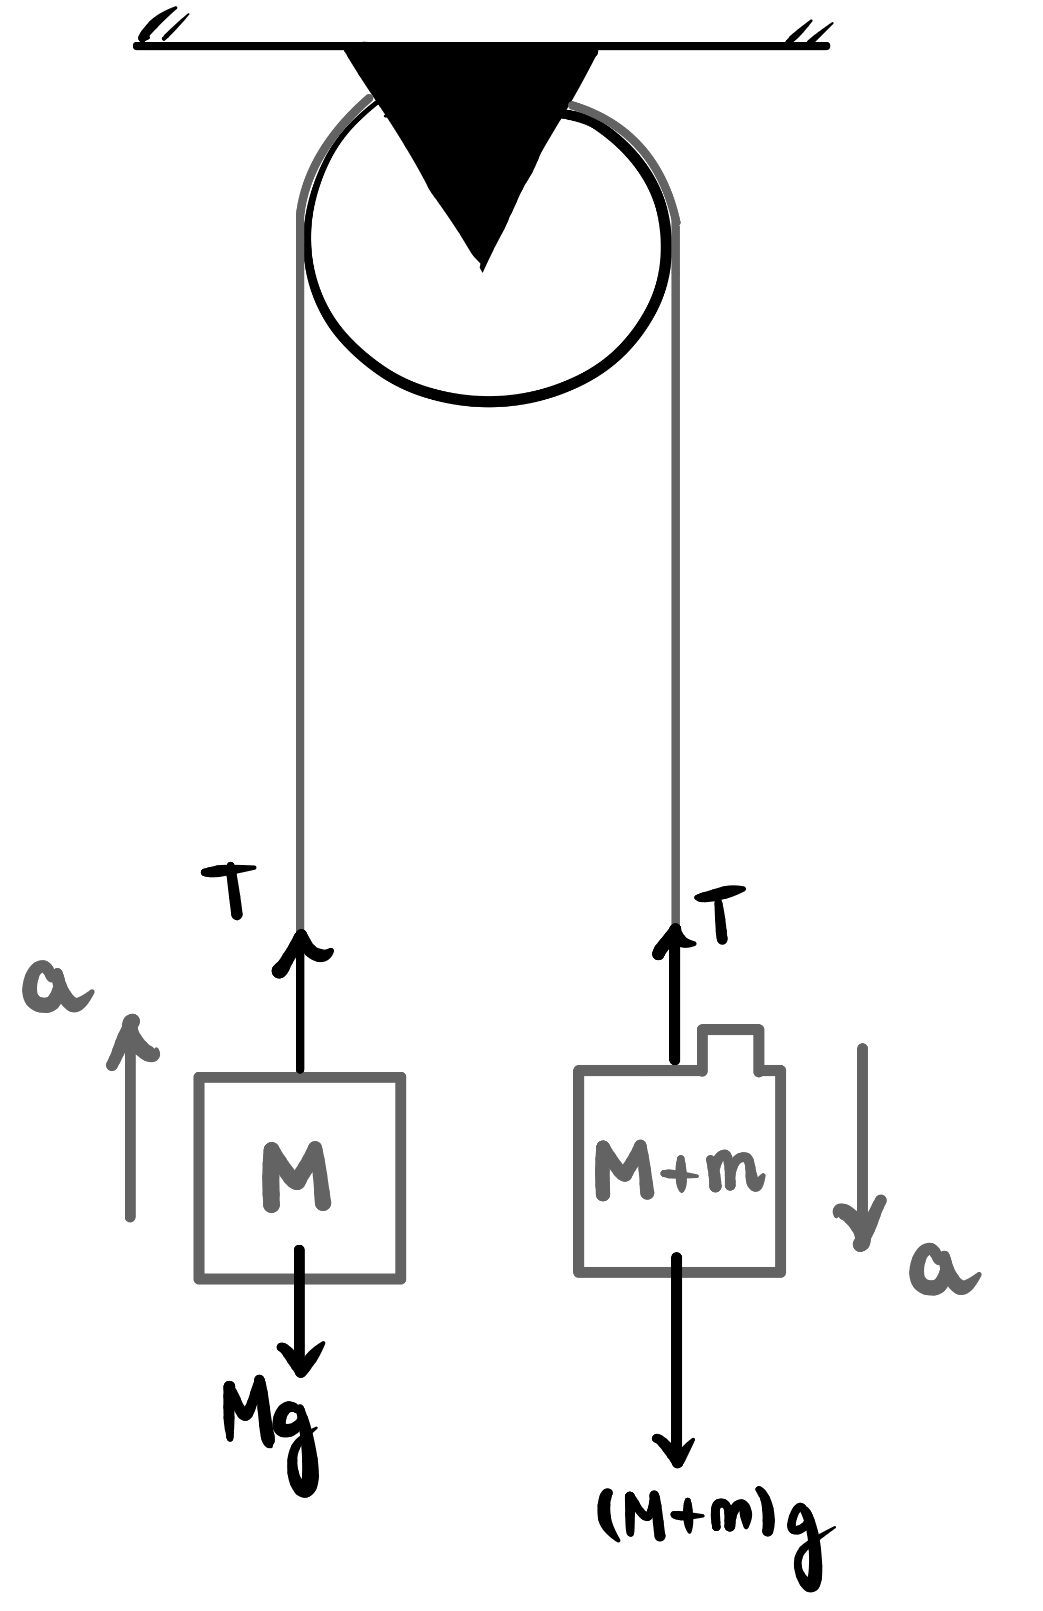
\includegraphics[width=0.22\linewidth]{imagensdinamicanewton/newtonpoliafixaexemploita.png}};
  \end{scope}
\end{tikzpicture}
\captionof{figure}{}
\label{fig_mec_newtonpoliafixaexemploita}
} 
\vspace{0.3cm}


Sendo assim, o cálculo da aceleração $a$ do sistema se dá através da aplicação da Segunda Lei de Newton:

\begin{align}
    \text{Bloco de massa $M$:}& \quad T - Mg = Ma \nonumber \\
    \text{Bloco de massa $(M+m)$:}& \quad (M+m)g - T  = (M+m)a, \nonumber
\end{align}

\noindent que, somando, nos leva a

$$ a = \dfrac{mg}{(2M+m)}.$$

Munidos de tal valor, avaliemos agora as forças que atuam exclusivamente no bloco de massa $m$: o seu peso $P=mg,$ vertical e para baixo; e a normal $N$ trocada com o bloco de massa $M$, que atua verticalmente para cima. Assim, a resultante de tais forças deve gerar no bloquinho a mesma aceleração $a$ que o sistema inteiro possui:

$$F_\text{R} = ma \implies mg - N = m \cdot \dfrac{mg}{(2M+m)} \implies \boxed{N = \dfrac{2Mm}{(2M+m)}g \implies \text{letra A}.}$$

\end{exemplo}







\begin{secnivel}[Força na Polia Móvel]{I}{Força na Polia Móvel}
  
  \eqLdois{dem}{eq_newton_poliamovel}{F_\text{FINAL}=F \cdot2^n}

\end{secnivel}






\secgfe{De onde vem}


A Equação \eqref{eq_newton_poliamovel} mostra como varia uma força $F$, aplicada na extremidade de um sistema de polias à medida que passa por cada polia móvel. Em tal equação, $n$ é o número de polias móveis, $F$ é a força feita por um agente em uma extremidade, como indica a Figura \ref{fig_mec_poliamoveldemonstracao}, e $F_\text{FINAL}$ é a força final que chegará no bloco na última extremidade. 

Em bom português, a Equação \eqref{eq_newton_poliamovel} diz que a força feita pelo menino dobra de valor a cada nova polia móvel no sistema.

\vspace{0.3cm}
{
\centering
\begin{tikzpicture}
  \begin{scope}[blend mode=multiply]
    \node {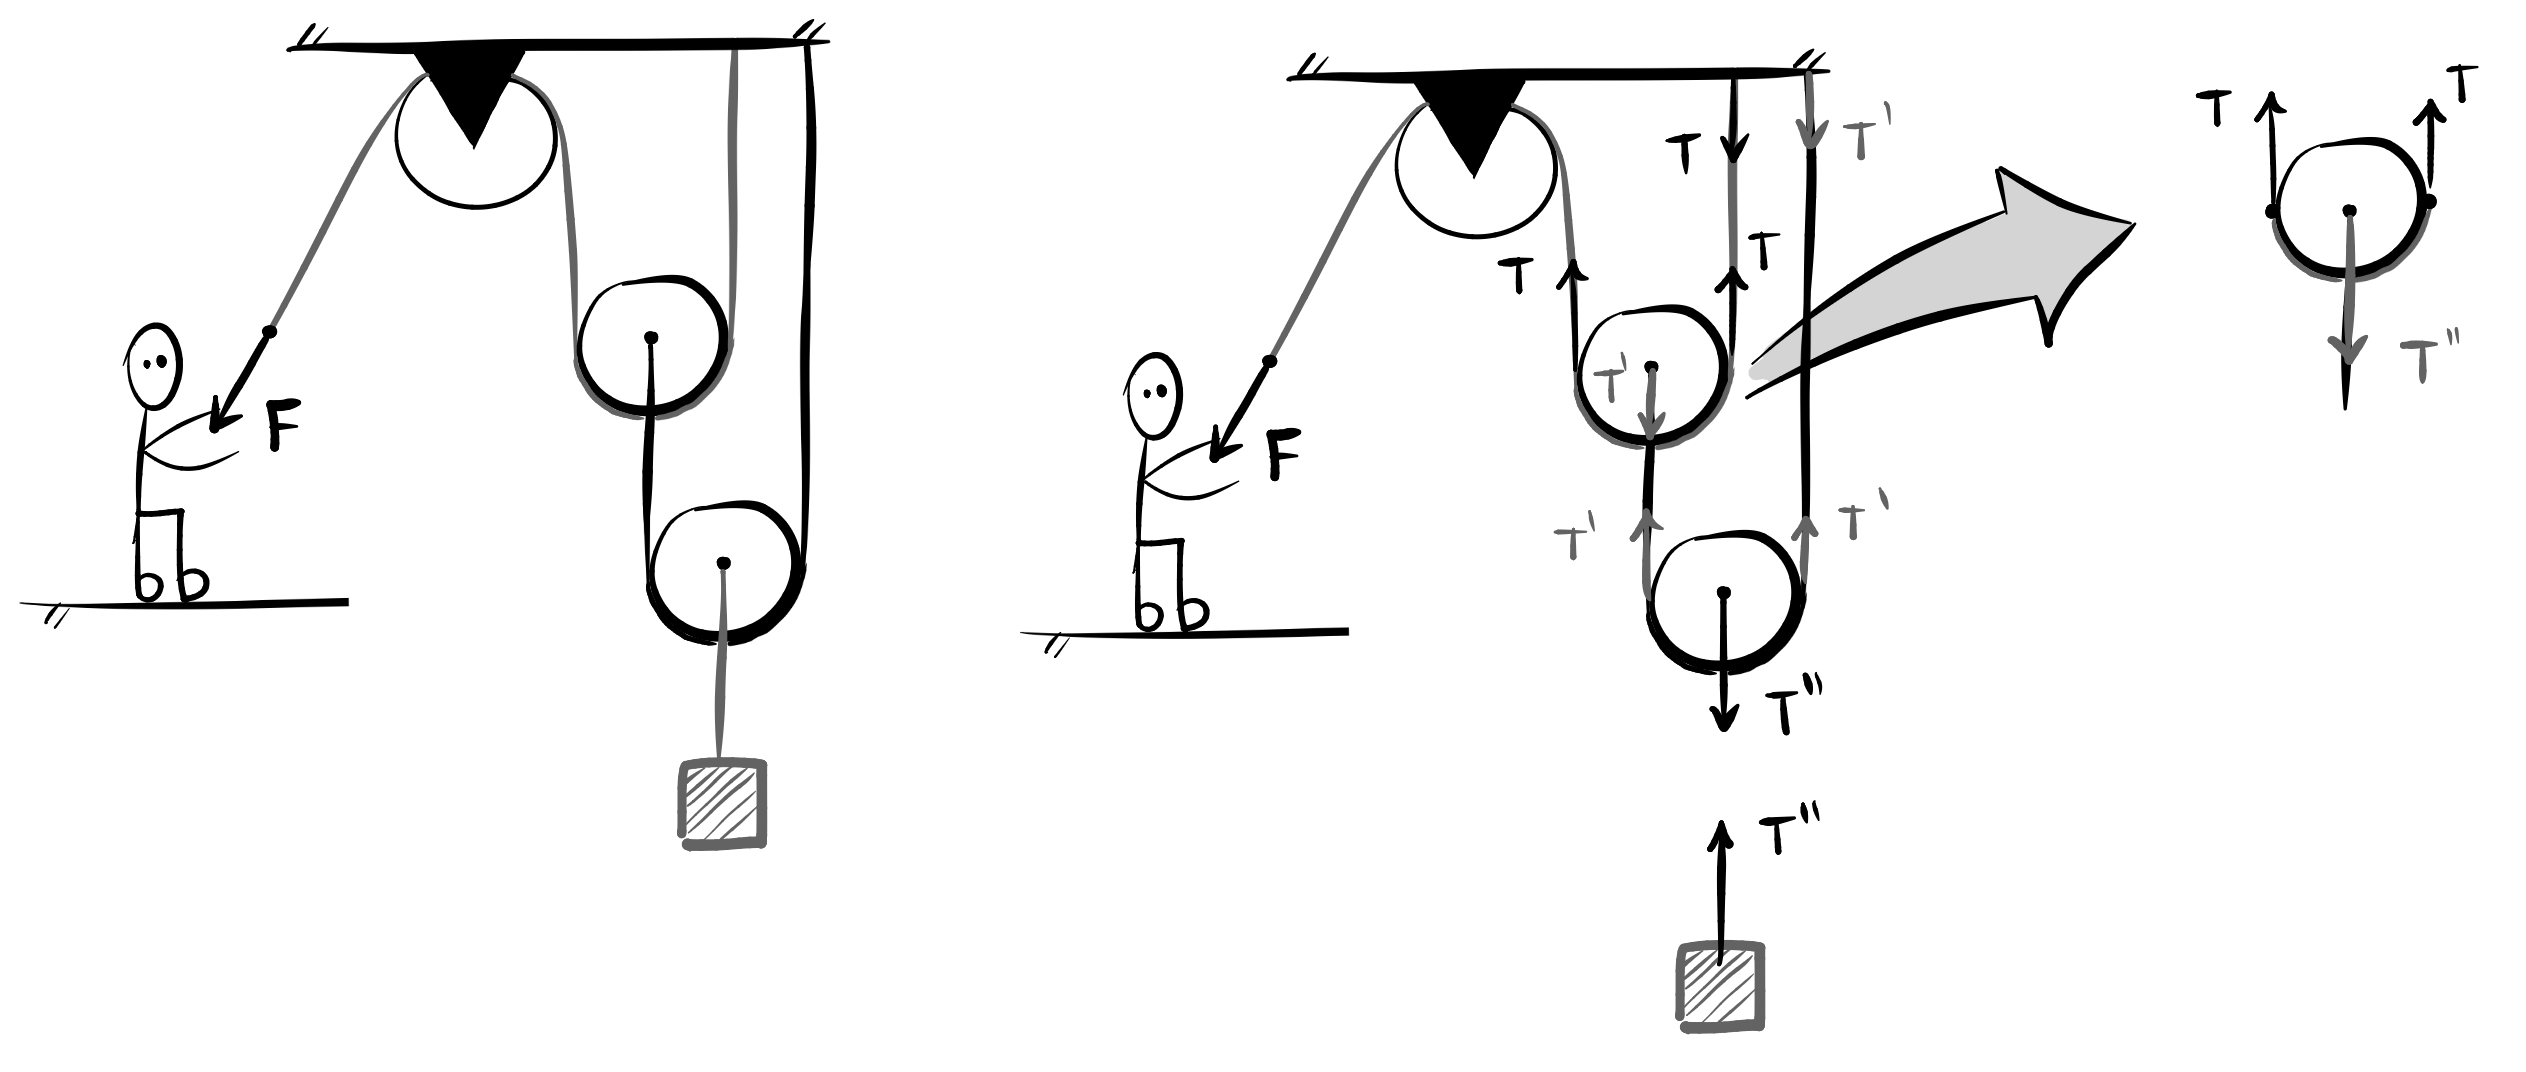
\includegraphics[width=0.8\linewidth]{imagensdinamicanewton/poliamovelprovamatematica.png}};
  \end{scope}
\end{tikzpicture}
\captionof{figure}{Entendendo o sistema de polias móveis.}
\label{fig_mec_poliamoveldemonstracao}
} 
\vspace{0.3cm}

Para entender porque isso funciona assim, é preciso recapitularmos duas ideias centrais:

\begin{enumerate}
    \item [(i)] A força de tração ao longo de um fio ideal é sempre a mesma. Isso vale sempre ao longo de um mesmo fio, e foi demonstrado no desenvolvimento da Equação \eqref{eq_newton_terceiraleinewton}.

    \item [(ii)] Uma polia ideal (que é o que sempre teremos) é aquela em que sua massa é tão pequena que a consideramos nula, isto é, $m_p \approx 0.$ Isso já foi levantado no desenvolvimento da Equação \eqref{eq_newton_poliafixa}.
\end{enumerate}

Note, no sistema da Figura \ref{fig_mec_poliamoveldemonstracao}, que temos uma polia fixa, presa ao teto, e na sequência duas polias móveis. As polias móveis são aquelas que, como o próprio nome diz, não estão fixadas de forma rígida em nenhuma parede e, portanto, podem se mover. Perceba que os fios que passam por tais polias estão presos no teto, mas as polias em si não o estão, de modo que possuem liberdade para se mover.

Note, também, que existem diversos fios no sistema: o primeiro é aquele que o menino puxa. Ele vai das mãos do menino, passa pela polia fixa, depois passa pela polia móvel e se prende no teto. Ao longo de todo esse fio, por ser ideal, a tração será sempre a mesma: $T=F$, como mostra a segunda imagem da figura.

O segundo fio é aquele que conecta o centro da primeira polia móvel, passa pela segunda polia móvel e se prende no teto. Como mudamos o fio, a tração já não tem nenhuma obrigatoriedade de ser manter a mesma. Chamemo-la de $T',$ o que está representando na segunda imagem da figura: ao longo de todo este fio a tração é sempre $T'.$

O terceiro fio seria aquele fio retilíneo que conecta a segunda polia móvel ao bloco. Novamente, como trata-se um novo fio, a tração pode assumir um outro valor -- que será sempre a mesma ao longo de tal fio. Chamemos tal valor de $T'',$ o que está representando na segunda imagem da figura.

Agora que compreendemos os diferentes fios e nomeamos as forças em cada um deles, vamos analisar a Segunda Lei de Newton para a primeira polia móvel, como destacado no último desenho à direita da Figura \ref{fig_mec_poliamoveldemonstracao}. Se a força $F$ aplicada pelo menino for suficiente para erguer o bloco, tal polia irá acelerar verticalmente para cima, uma vez que o sistema como um todo é puxado para cima. Digamos que a aceleração da polia de massa $m_p$ é $a_p.$ Assim, pela Segunda Lei de Newton, teremos, para a primeira polia móvel:

$$ F_{\text{R}} = m a \implies 2T - T'= \cancelto{0}{m_p} \cdot a_p \implies  2T - T' = 0 \implies \boxed{T'= 2T.}$$

Ou seja, ainda que a polia esteja acelerando junto ao bloco, por ter massa nula, a Segunda Lei de Newton nos diz que, em uma polia ideal, a força resultante sempre será zero. Para tal, é necessário que a tração no novo fio logo abaixo da polia móvel seja o dobro da tração no fio superior, a fim de fazer com que a resultante das forças na polia móvel seja nula. A mesma análise para a segunda polia móvel nos levaria a concluir que $T''= 2T',$ ou seja, a força dobraria novamente ao se passar por uma polia móvel.

Dizemos, portanto, que um sistema com polias móveis oferece vantagem mecânica: a força se multiplica por 2 a cada nova polia móvel no sistema, fazendo com que, por meio da aplicação de uma pequena força $F$ em um extremo, seja possível erguer corpos extremamente massivos no outro extremo, bastando para isso adicionar um número suficiente de polias móveis capaz de fazer a força dobrar até conseguir superar o peso de tal corpo.

Desse modo, ao fazer uma força $F$ em um fio na extremidade de um sistema com várias polias móveis, a força irá multiplicar por 2 a cada polia móvel pela qual passar, de modo que a força final que teremos no extremo será

$$ F_\text{FINAL}=F\cdot  \underbrace{2 \cdot 2 \cdot 2 \dots \cdot 2}_{\text{n vezes}} = F \cdot 2^n, $$

\noindent que é exatamente o que diz a Equação \eqref{eq_newton_poliamovel}.


\secgfe{Onde é usada}

Os contextos mais comuns de aplicação aqui são os mesmos daqueles da polia fixa: aparelhos de academia ou dispositivos em que se deseja carregar grandes massas. Aqui, como temos um dispositivo que oferece vantagem mecânica, ele é particularmente interessante para carregar objetos extremamente pesados, o que poderá ser feito por meio da aplicação de pequenas forças, como a Equação \eqref{eq_newton_poliamovel} indica.

Considere, por exemplo, a situação da Figura \ref{fig_mec_poliamovelteoria}. Qual seria a força necessária a ser feita para carregar o bloco de massa $m=10kg$ com velocidade constante?

\vspace{0.3cm}
{
\centering
\begin{tikzpicture}
  \begin{scope}[blend mode=multiply]
    \node {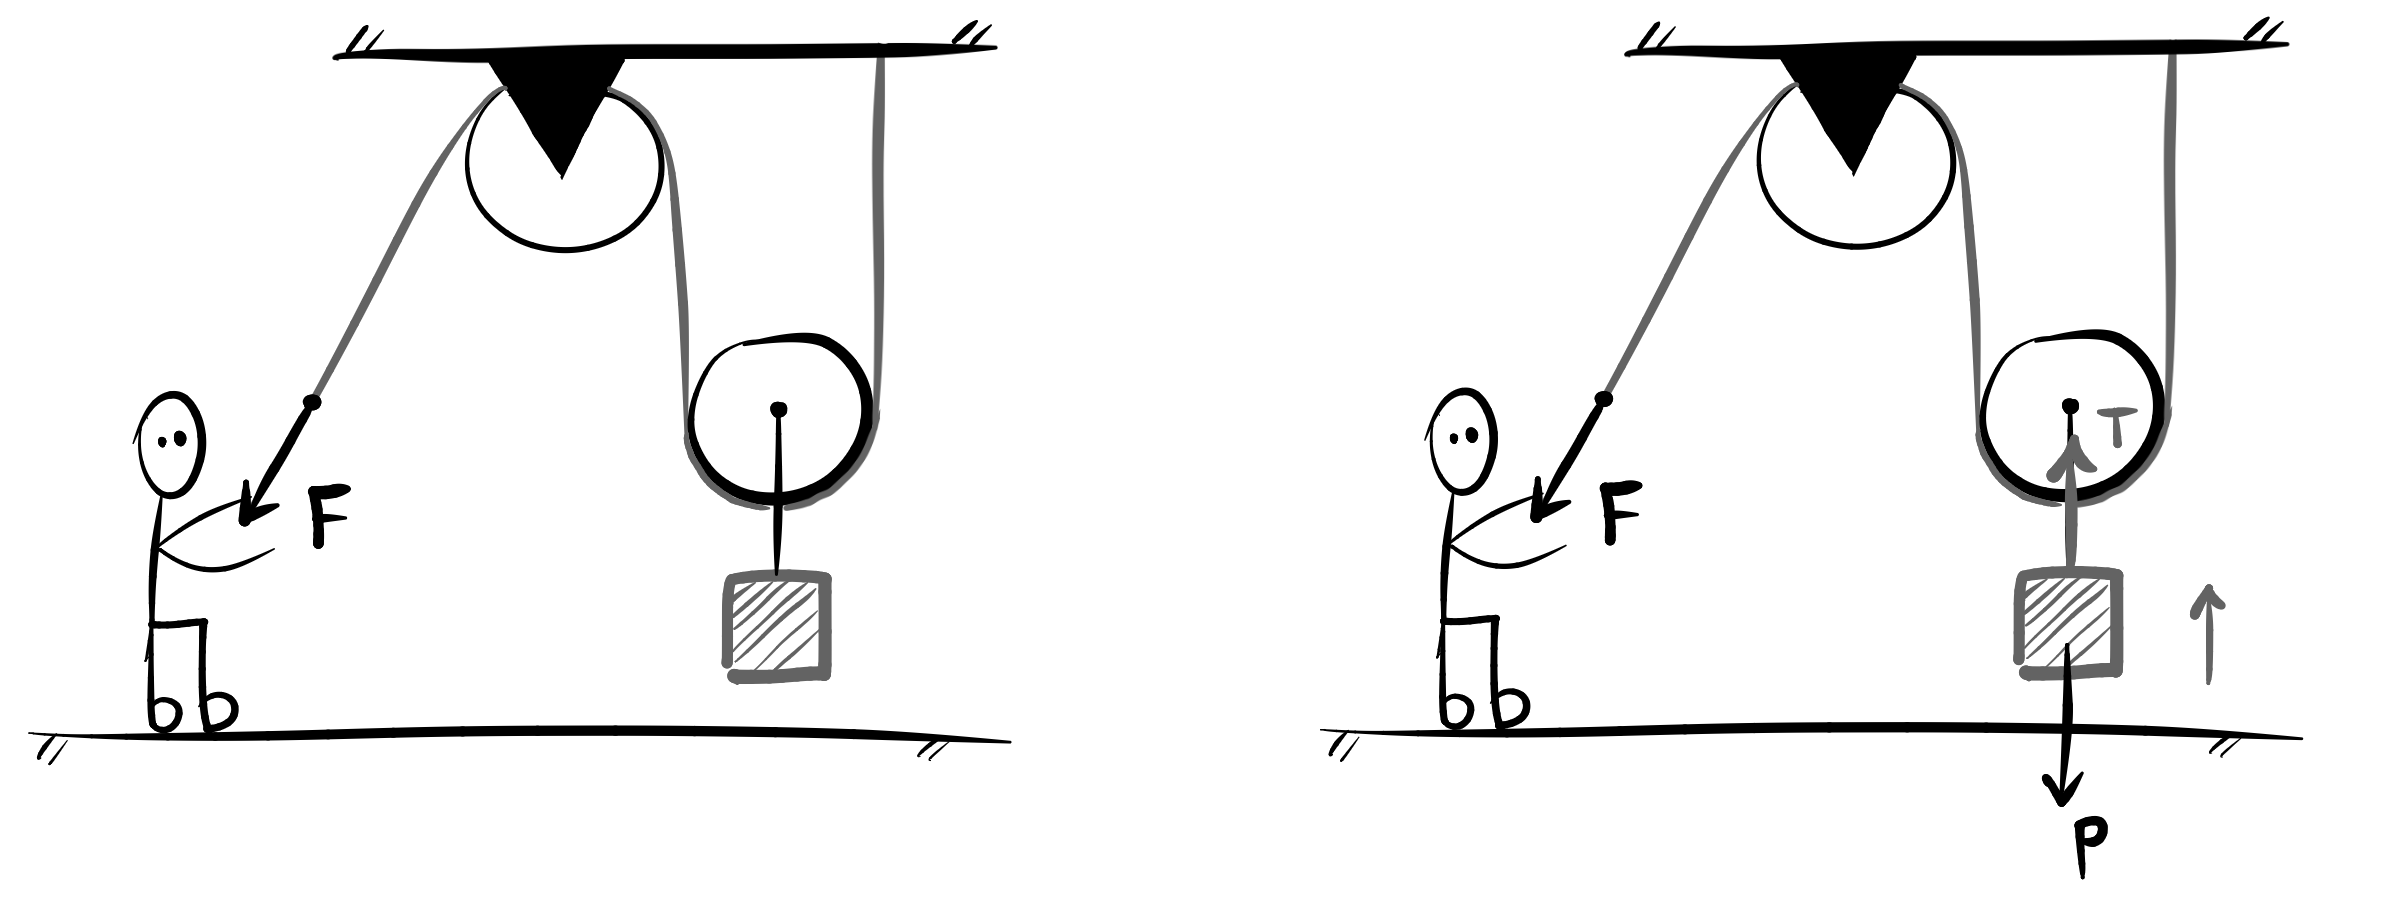
\includegraphics[width=0.6\linewidth]{imagensdinamicanewton/poliamovelteoria.png}};
  \end{scope}
\end{tikzpicture}
\captionof{figure}{Erguendo bloco com um sistema de polias.}
\label{fig_mec_poliamovelteoria}
} 
\vspace{0.3cm}

Para subir com velocidade constante o bloco estará em equilíbrio, isto é, $F_\text{R}=0.$ Como mostra a segunda imagem da Figura \ref{fig_mec_poliamovelteoria}, isso quer dizer que $T=P=100$N. Como a força feita pelo menino na extremidade da direita irá dobrar a cada polia móvel -- e temos apenas uma polia móvel -- ele pode fazer uma força de apenas $50$N, que se manterá constante ao longo da polia fixa e dobrará de valor após passar pela polia móvel, originando a força de $100$ N para erguer a caixa com velocidade constante.

Parece mágica em um primeiro momento: é possível erguer um bloco de 10kg fazendo a força que seria necessária para erguer um bloco de 5kg. Mas não tem nada de errado nisso: não existe, na Física, nenhuma \textit{lei de conservação da força}, de modo que um sistema que multiplique o valor da força e ofereça vantagem mecânica, como o sistema de uma polia móvel, é perfeitamente viável e fisicamente possível, por mais que cause um certo estranhamento em um primeiro momento. Veremos, ao estudar a Lei de Conservação da Energia, que tal sistema não só é possível como também deve ser exatamente desse modo, a fim de respeitar tal lei da Física.


\secgfe{Erros comuns}

Em geral os problemas irão envolver polias fixas e móveis na mesma situação. O erro mais comum é o estudante não conseguir identificar quais são as polias fixas e quais são as móveis, e acabar usando que a força dobra ao passar por uma polia fixa, por exemplo.

Note, na Figura \ref{fig_mec_roldanafixaemovel}, que todas as quatro polias da parte de cima estão fixas no teto, logo, tratam-se de polias fixas, sem vantagem mecânica. Já as quatro polias da parte inferior são móveis -- elas não estão fixas\footnote{Algum leitor poderia pensar \textit{``ora, mas elas estão fixadas na barra abaixo, que está presa ao bloco.''} Sim, mas perceba que o bloco não está fixado em lugar algum, logo, todo esses sistema -- polias, barra e bloco -- pode se mover. Portanto, tratam-se de polias móveis. Se um objeto está fixado em um corpo que pode se mover, logo, tal objeto também poderá se mover, sendo, portanto, um corpo móvel e não fixo.} e podem se mover junto com o bloco.

\vspace{0.3cm}

{
\centering
\begin{tikzpicture}
  \begin{scope}[blend mode=multiply]
    \node {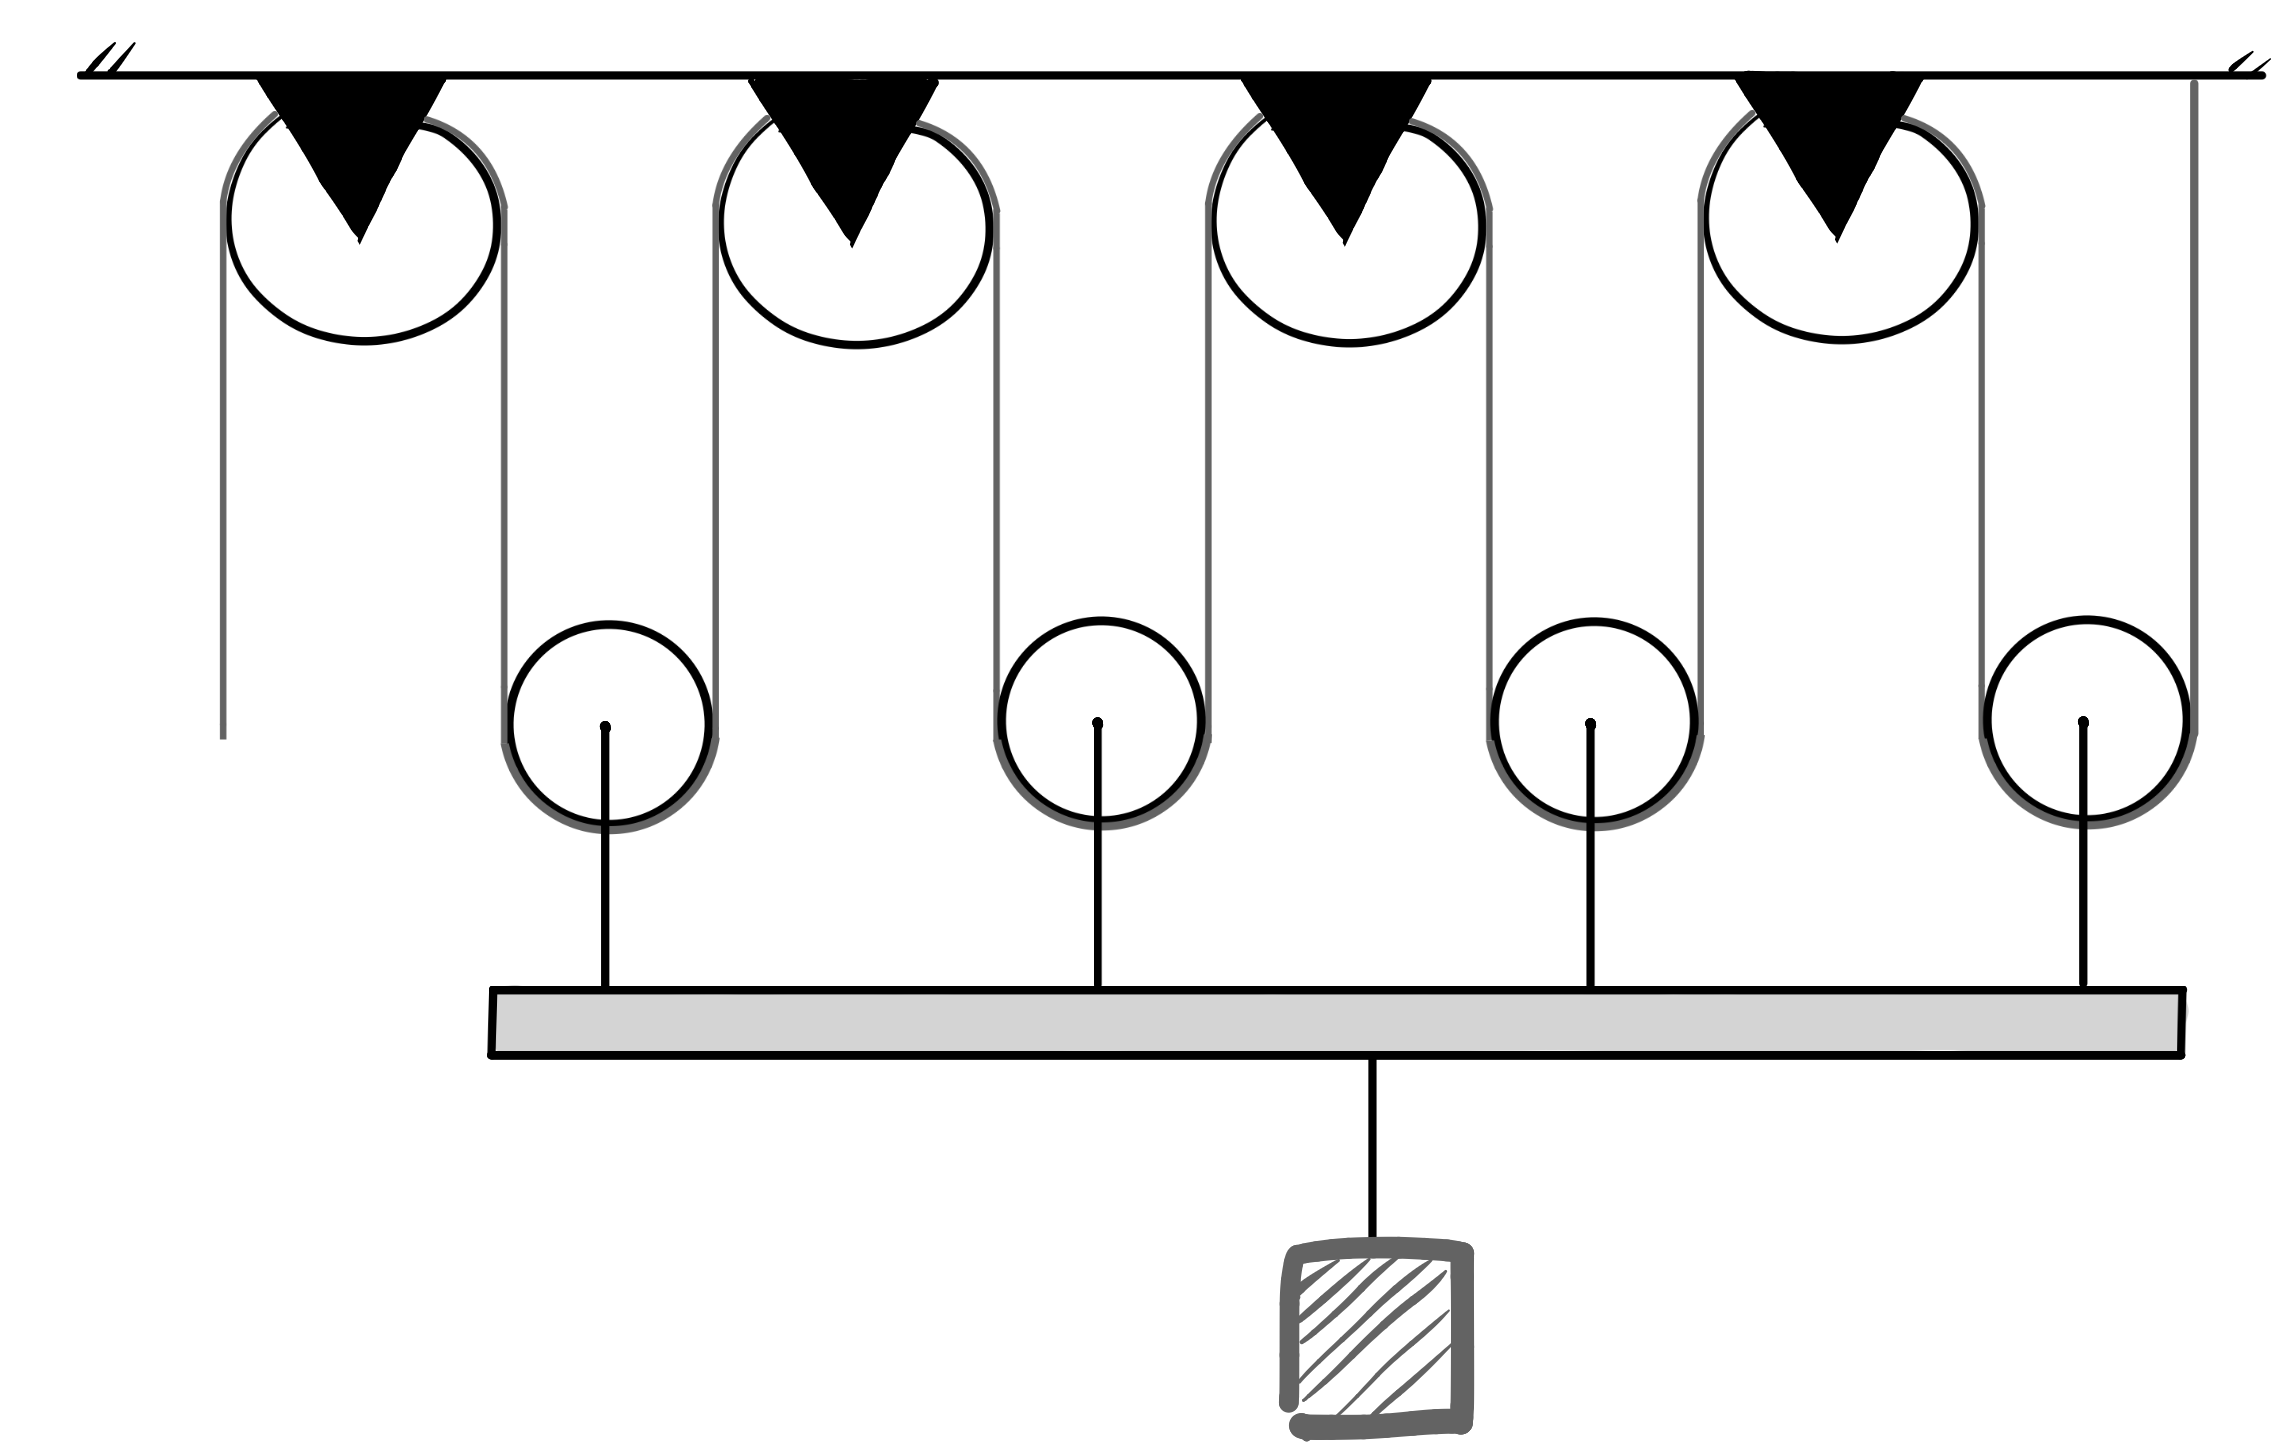
\includegraphics[width=0.45\linewidth]{imagensdinamicanewton/roldanafixaemovel.png}};
  \end{scope}
\end{tikzpicture}
\captionof{figure}{Roldanas fixas e móveis.}
\label{fig_mec_roldanafixaemovel}
} 
\vspace{0.3cm}



\secgfe{Observações}

Vamos discorrer brevemente sobre a razão pela qual o sistema multiplicador de forças é fisicamente possível. Isso será entendido com mais profundidade ao estudarmos o princípio da Conservação da Energia Mecânica, no estudo da Equação \eqref{eq_energia_conservacaodaenergiamecanica}.


Observe a situação da Figura \ref{fig_mec_poliamovelconservacao}. Tal situação mostra que, ao puxar o fio e fazer com que a polia móvel (e, consequentemente, o bloco, uma vez que este está preso em tal polia por um fio) se mova para cima de um certo tanto $x$, foi necessário que o menino puxasse o fio do dobro desse valor, isto é, de $2x$. Isso ocorre porque o fio sai da polia fixa, desce pela esquerda da polia móvel e sobe pela sua direita, prendendo-se ao teto. Sendo assim, ao puxar o fio de 2 metros, por exemplo, será como se tivéssemos puxado 1 metro da parte esquerda e 1 metro da parte direita. Ou seja, o sistema só sobe 1 metro, ainda que se puxe 2 metros de fio.




\vspace{0.3cm}
{
\centering
\begin{tikzpicture}
  \begin{scope}[blend mode=multiply]
    \node {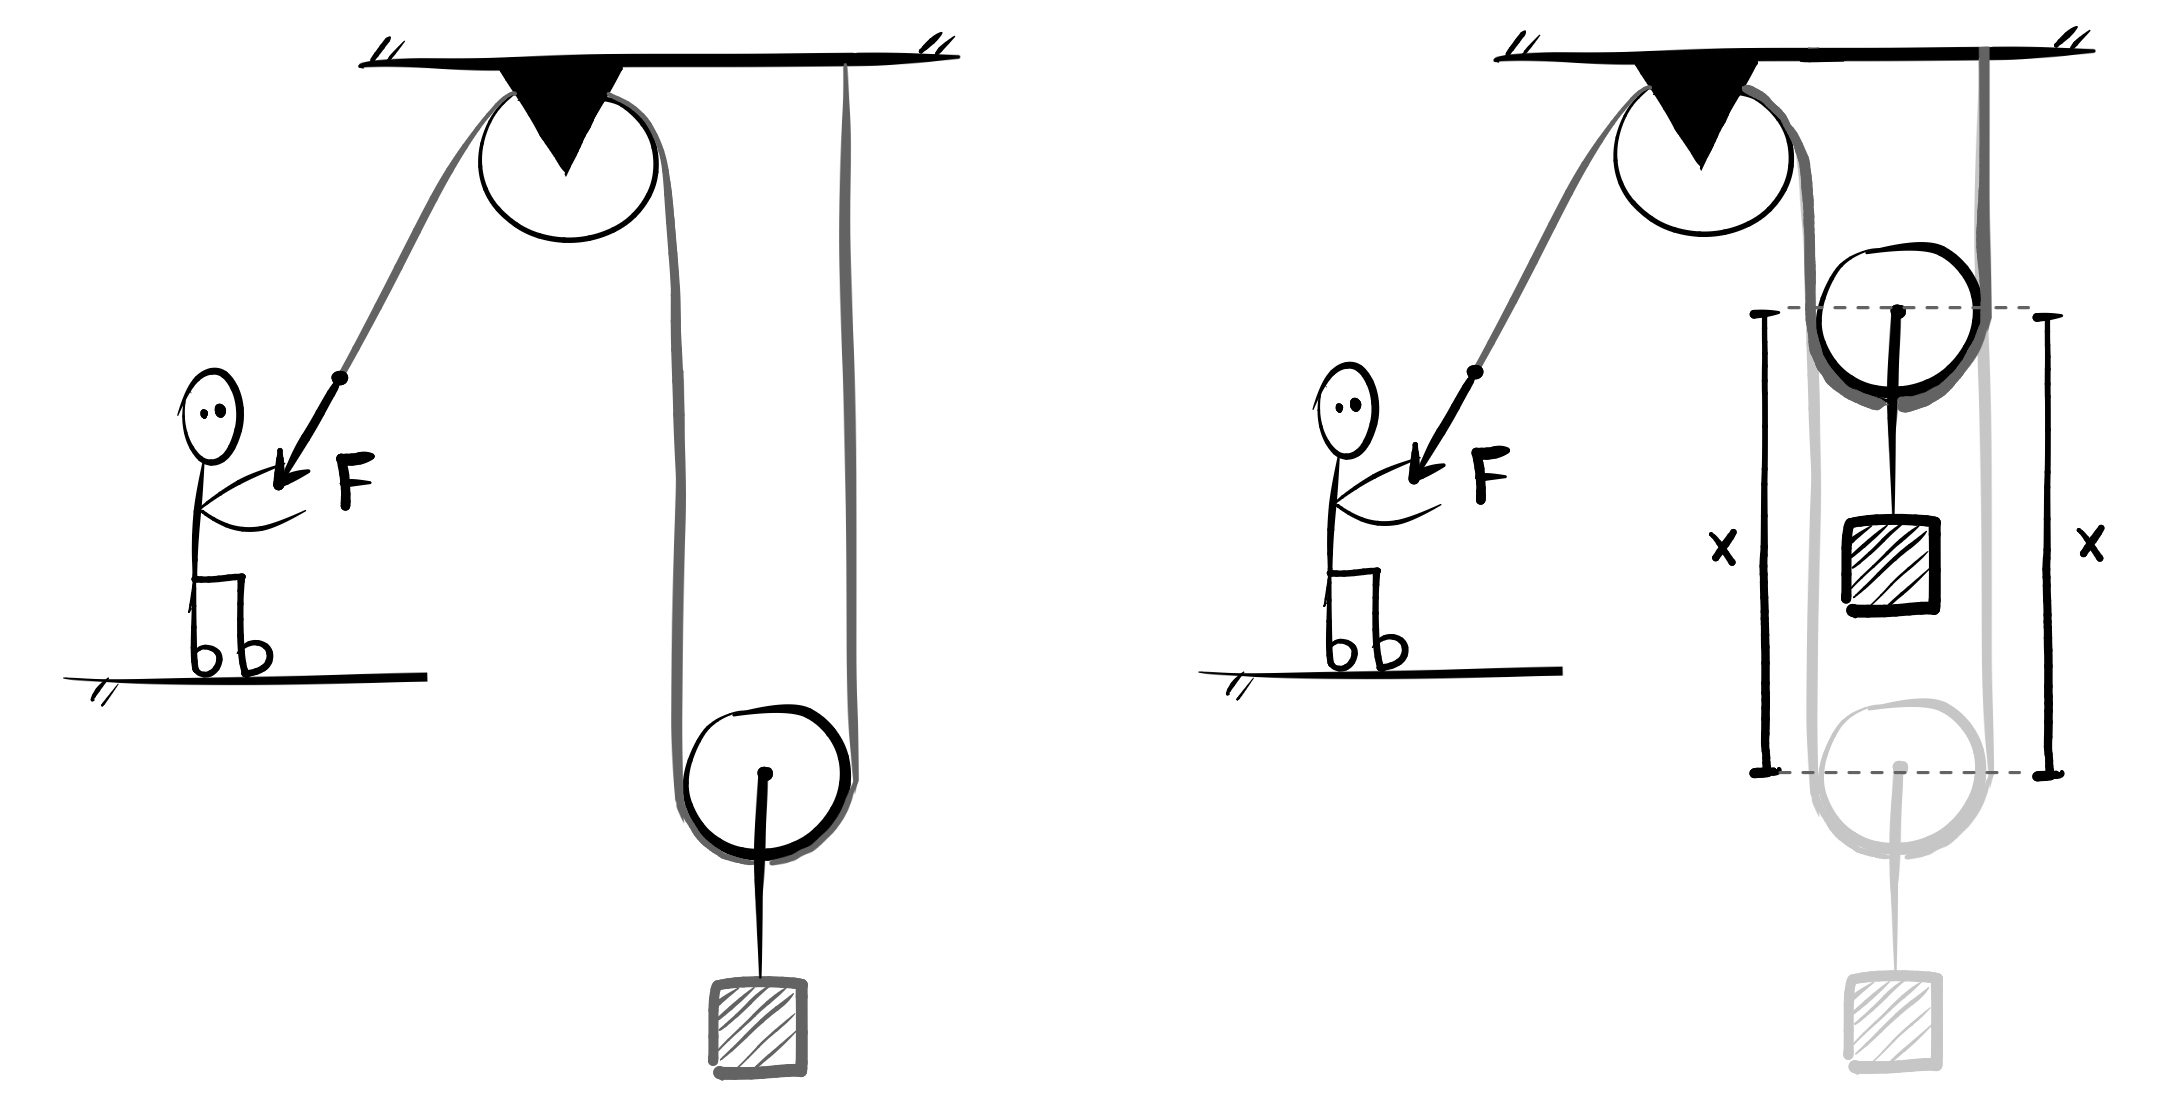
\includegraphics[width=0.6\linewidth]{imagensdinamicanewton/poliamoveleconservacaoenergia.png}};
  \end{scope}
\end{tikzpicture}
\captionof{figure}{O preço a se pagar neste sistema: para erguer o bloco de um tanto $x$ é preciso puxar o dobro de corda, isto é, $2x$.}
\label{fig_mec_poliamovelconservacao}
} 
\vspace{0.3cm}

No final do dia esse é o preço que se paga em um sistema como esse, nada é de graça: a força feita pelo menino é metade da força que chega ao bloco, porém a quantidade de fio que o menino deve puxar será sempre o dobro do tanto que o bloco se move. Assim, o menino precisará puxar a corda sempre com o dobro da velocidade com que o bloco se moverá: para subir o bloco a uma velocidade de 3 m/s é preciso que o menino puxe 6 metros de corda a cada segundo. 

Como veremos no estudo da Equação \eqref{eq_energia_conservacaodaenergiamecanica}, o produto da força feita pelo tanto de fio que se puxa (seu deslocamento) é justamente igual à energia dispendida pelo menino. Logo, ele faz metade da força, mas puxa o dobro de corda, de modo que a energia que ele gasta é exatamente a mesma que chega ao bloco e o suspende.

Assim, apesar de se fazer menos força, o esforço (energia dispendida) é o mesmo. Troca-se fazer menos força por puxar mais corda -- o que, em muitos casos, é uma excelente troca.


\vspace{0.3cm}


\begin{exemplo}[Nível I (EsPCEx 2020)]\label{exemplo_newton_poliamovel0}

O sistema de polias, sendo uma fixa e três móveis, encontra-se em equilíbrio estático, conforme mostra o desenho. 
A constante elástica da mola, ideal, de peso desprezível, é igual a $50\,\text{N/cm}$ e a força $F$ na extremidade da corda é de intensidade igual a $100\,\text{N}$. 
Os fios e as polias, iguais, são ideais.

\vspace{0.3cm}
{
\centering
\begin{tikzpicture}
  \begin{scope}[blend mode=multiply]
    \node {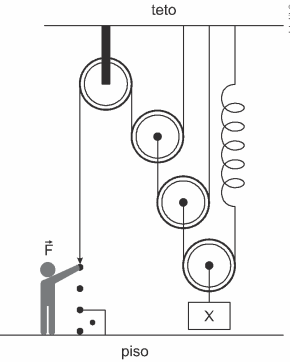
\includegraphics[width=0.27\linewidth]{imagensdinamicanewton/poliamovelexemplo2.png}};
  \end{scope}
\end{tikzpicture}
\captionof{figure}{}
\label{fig_mec_poliamovelexemplo2}
} 
\vspace{0.3cm}

O valor do peso do corpo $X$ e a deformação sofrida pela mola são, respectivamente,
\begin{enumerate}
    \item [a)]$800\,\text{N}$ e $16\,\text{cm}$
    \item [b)]$400\,\text{N}$ e $8\,\text{cm}$
    \item [c)]$600\,\text{N}$ e $7\,\text{cm}$
    \item [d)]$800\,\text{N}$ e $8\,\text{cm}$
    \item [e)]$950\,\text{N}$ e $10\,\text{cm}$
\end{enumerate}

\resolucao

A força $F$ feito pelo menino irá dobrar a cada polia móvel pela qual passar, de modo que, para 3 polias móveis, a força final será

$$ F_\text{FINAL} = F \cdot 2^3 = 8F = 8 \cdot 100 = 800 \text{N.}$$

Assim, se o bloco está em equilíbrio, é porque tal força é exatamente igual ao seu peso: $P=800 \text{N}.$

O fio que possui tração de 800 N é aquele que conecta o bloco à última polia. Logo, o fio em que a mola está conectada é outro: ao longo deste fio a tração é de 400N. Observe em detalhes o diagrama das forças na Figura \ref{fig_mec_poliamoveldemonstracao} em caso de dúvida.

Assim, para a mola, teremos:

$$F = kx \implies 400 = 50x \implies x = 8 \text{ cm},$$

\noindent de modo que a letra D é a resposta correta.


\end{exemplo}



\vspace{0.3cm}


\begin{exemplo}[Nível II]\label{exemplo_newton_poliamovel02}

Considere o sistema da Figura \ref{fig_mec_poliamovelexemploresolvido21}. Qual deve ser o valor da massa $M$ para que ela fique em equilíbrio?

\vspace{0.3cm}
{
\centering
\begin{tikzpicture}
  \begin{scope}[blend mode=multiply]
    \node {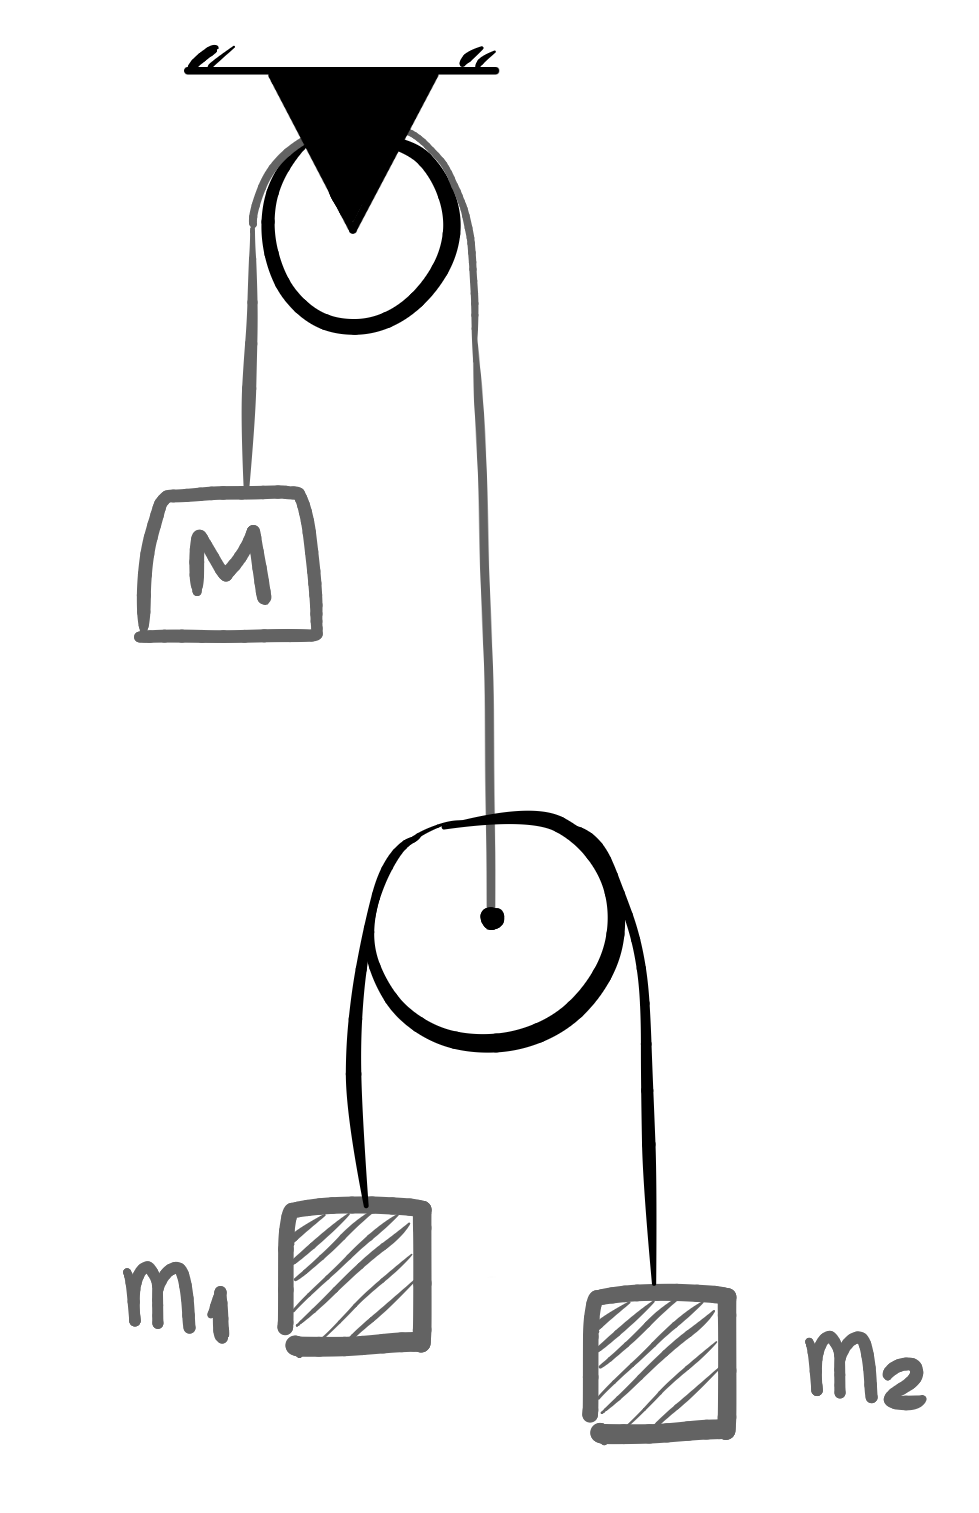
\includegraphics[width=0.22\linewidth]{imagensdinamicanewton/poliamovelexemploresolvido21.png}};
  \end{scope}
\end{tikzpicture}
\captionof{figure}{}
\label{fig_mec_poliamovelexemploresolvido21}
} 
\vspace{0.3cm}


\resolucao

O leitor mais ingênuo poderia pensar que a massa $M$ deveria equivaler à soma das massas do lado direito, isto é, $M = m_1+m_2.$ Isso até seria verdade se o sistema inteiro estivesse em equilíbrio, o que não ocorre.

\medskip

As massas da direita, $m_1$ e $m_2,$ certamente não estarão em equilíbrio se $m_1 \neq m_2$ elas certamente estarão acelerando. Queremos, contudo, que a polia móvel na qual elas estão conectadas permaneça em equilíbrio. Como acelerações são geradas por forças, o fato do sistema da direita estar acelerado irá alterar as trações nos fios, o que irá afetar a dinâmica do sistema e, portanto, irá alterar o valor de massa $M$ necessário para manter  a polia móvel em equilíbrio. 

\vspace{0.3cm}
{
\centering
\begin{tikzpicture}
  \begin{scope}[blend mode=multiply]
    \node {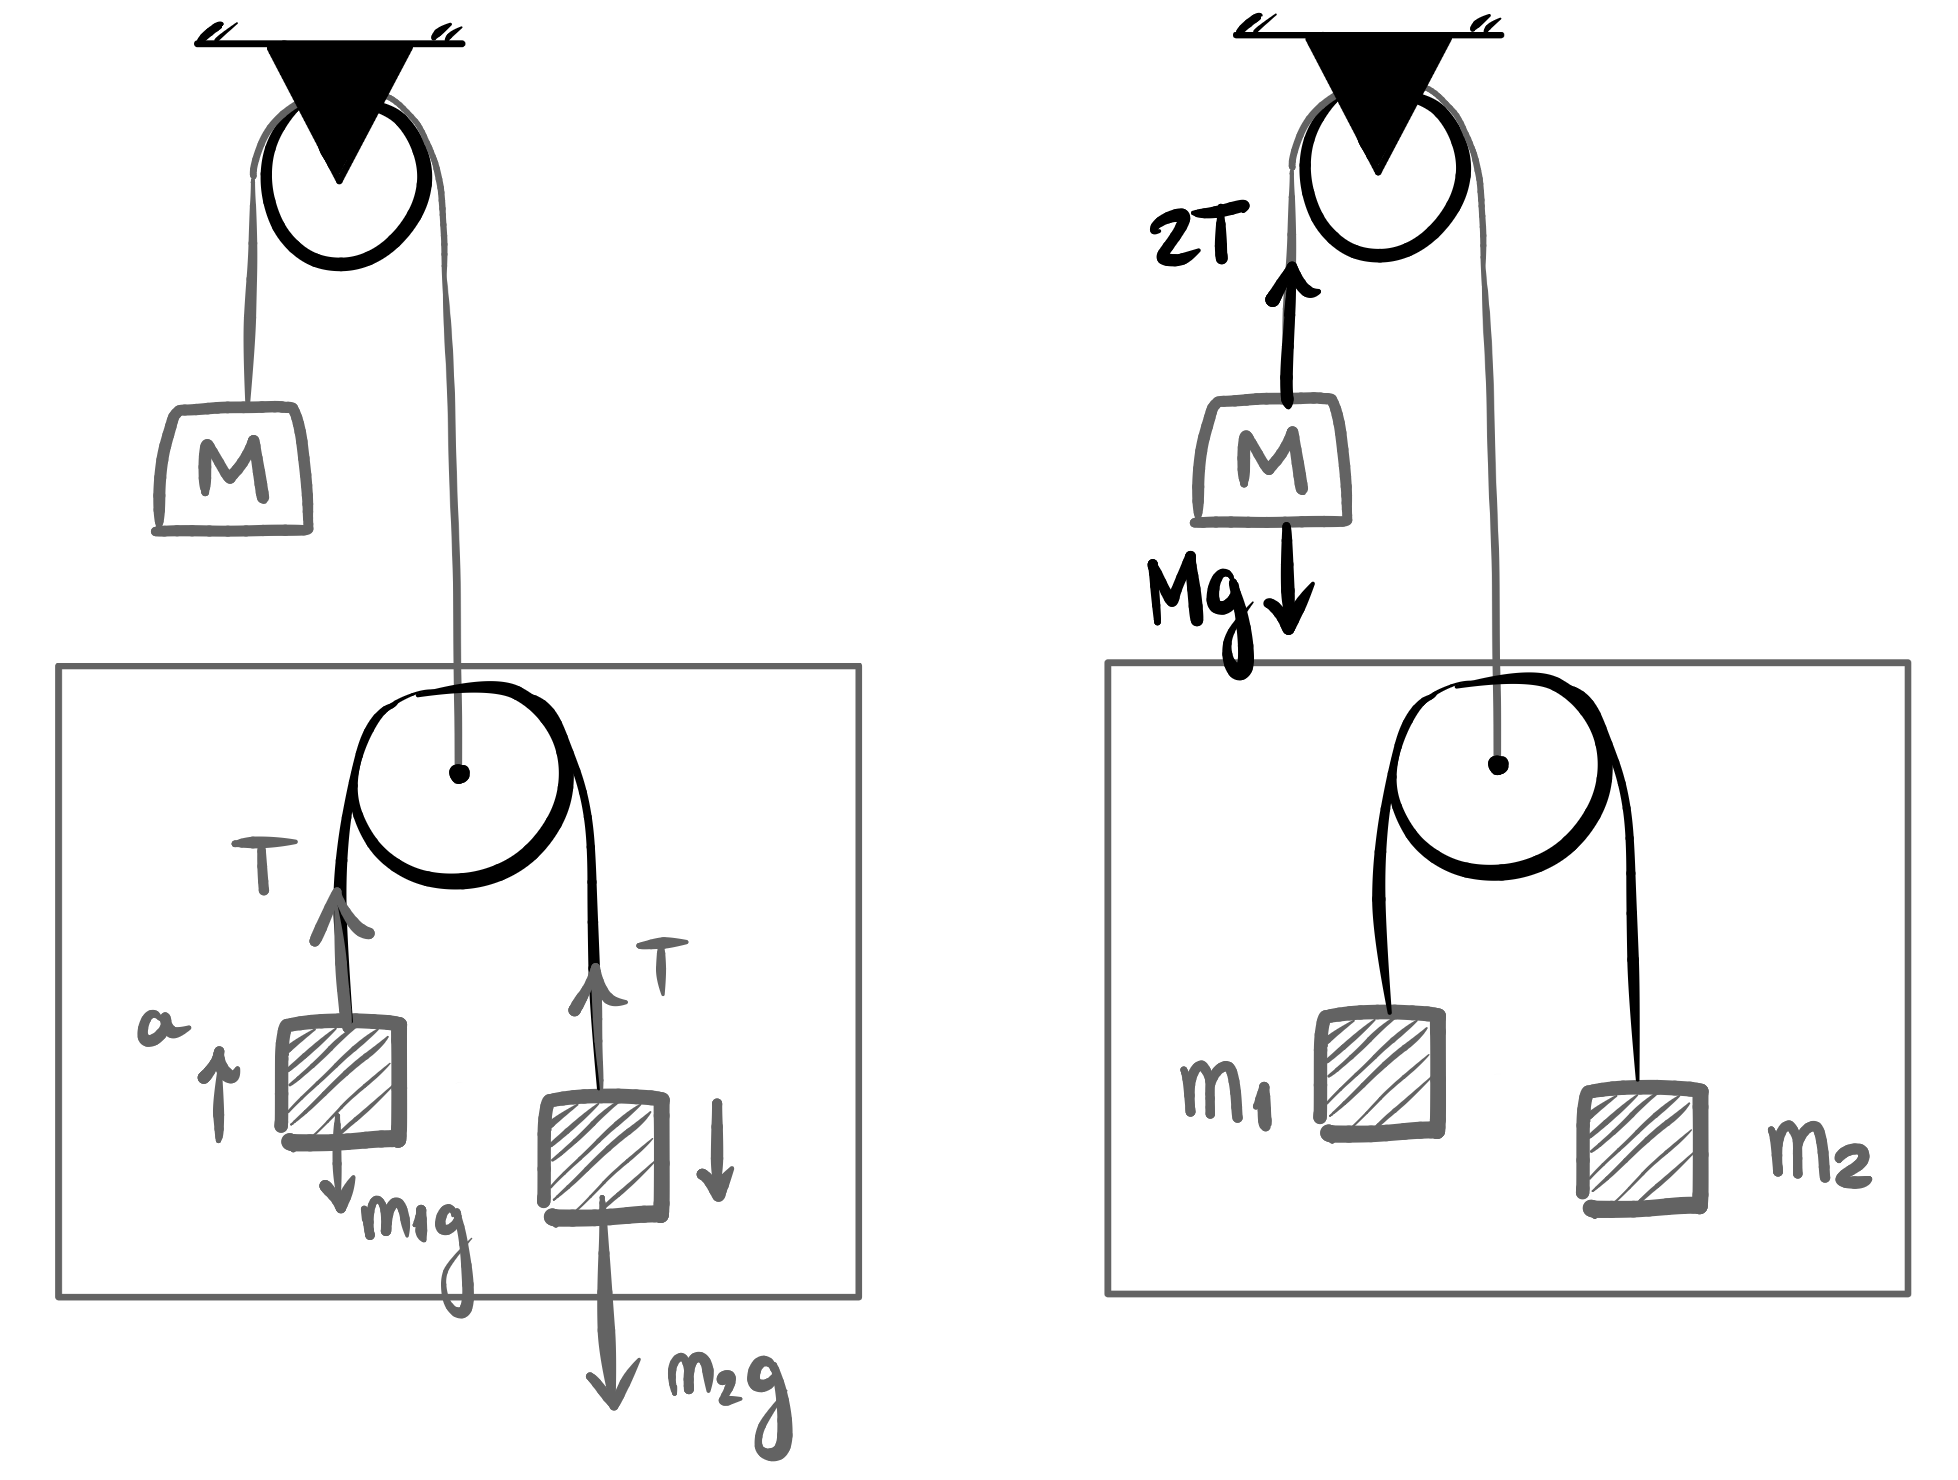
\includegraphics[width=0.6\linewidth]{imagensdinamicanewton/poliamovelexemploresolvido22.png}};
  \end{scope}
\end{tikzpicture}
\captionof{figure}{}
\label{fig_mec_poliamovelexemploresolvido22}
} 
\vspace{0.3cm}

Equacionando a Segunda Lei de Newton para as massas $m_1$ e $m_2,$ supondo $m_2>m_1$, teremos:

\begin{align}
    T - m_1g &= m_1 a \nonumber \\
    m_2g - T &= m_2 a ,\nonumber
\end{align}

\noindent que, somando, nos leva a

$$ a =  \left(\dfrac{m_2 - m_1}{m_2+m_1} \right)g \quad \text{ e } \quad T = \dfrac{2m_1m_2g}{m_1+m_2}.$$

A segunda imagem da Figura \ref{fig_mec_poliamovelexemploresolvido22} mostra que a força no fio que passa pelo bloco de massa $M$ é $2T,$ de modo que, para que ele fique em equilíbrio, é preciso que:

$$ 2T = Mg \implies \boxed{M = \dfrac{4m_1m_2}{m_1+m_2}.}$$

Note que, se $m_1 = m_2,$ teremos $a=0$ e $T = mg, $ como esperado. Neste caso os blocos da direita ficam parados ou em MRU -- de toda forma, se encontram em equilíbrio. Assim, a expressão acima se reduz a $M=2m=m+m,$ que foi nossa intuição inicial.

\medskip

Contudo, se o sistema da direita estiver acelerado, a força necessária a ser feita do lado esquerdo para manter a polia móvel em equilíbrio não será igual à soma dos pesos dos blocos $m_1$ e $m_2$, e sim igual ao peso de um bloco de massa $M=4m_1m_2/(m_1+m_2)$

\medskip 

Façamos uma breve discussão desse resultado. A média aritmética (MA) entre dois números $x_1$ e $x_2$ e sua média harmônica (MH) são definidas como:

$$ MA = \dfrac{x_1+x_2}{2} \quad \text{ e } \quad MH = \dfrac{2}{\dfrac{1}{x_1} + \dfrac{1}{x_2}}.$$

A desigualdade das médias nos diz que $MA \geq MH,$ a igualdade ocorrendo quando os números forem iguais. Logo, teremos:

$$ \dfrac{x_1+x_2}{2} \geq  \dfrac{2}{\dfrac{1}{x_1} + \dfrac{1}{x_2}},$$

\noindent o que se escreve como

$$ x_1+x_2 \geq \dfrac{4x_1x_2}{x_1+x_2}.$$

Fazendo $m_1$ e $m_2$ como sendo os números $x_1$ e $x_2$, teremos

$$ m_1+m_2 \geq \dfrac{4m_1m_2}{m_1+m_2} = M,$$

\noindent ou seja, se o sistema dos blocos $m_1$ e $m_2$ estiver acelerando, como na primeira imagem da Figura \ref{fig_mec_poliamovelexemploresolvido22}, então a massa $M$ que mantém a polia móvel em repouso será sempre menor que a soma das massas $m_1$ e $m_2.$ Ou seja, é mais fácil sustentar o sistema da máquina de Atwood acelerado do que o sistema em equilíbrio.


\end{exemplo}
\vspace{0.3cm}








\begin{exemplo}[Nível III]\label{exemplo_newton_poliamovel03}

O sistema da Figura \ref{fig_mec_poliamovelexemplo222a} é livre de atrito e os fios e polias são ideais. Se a gravidade local vale $g,$ encontre a aceleração de cada bloco.

\vspace{0.3cm}
{
\centering
\begin{tikzpicture}
  \begin{scope}[blend mode=multiply]
    \node {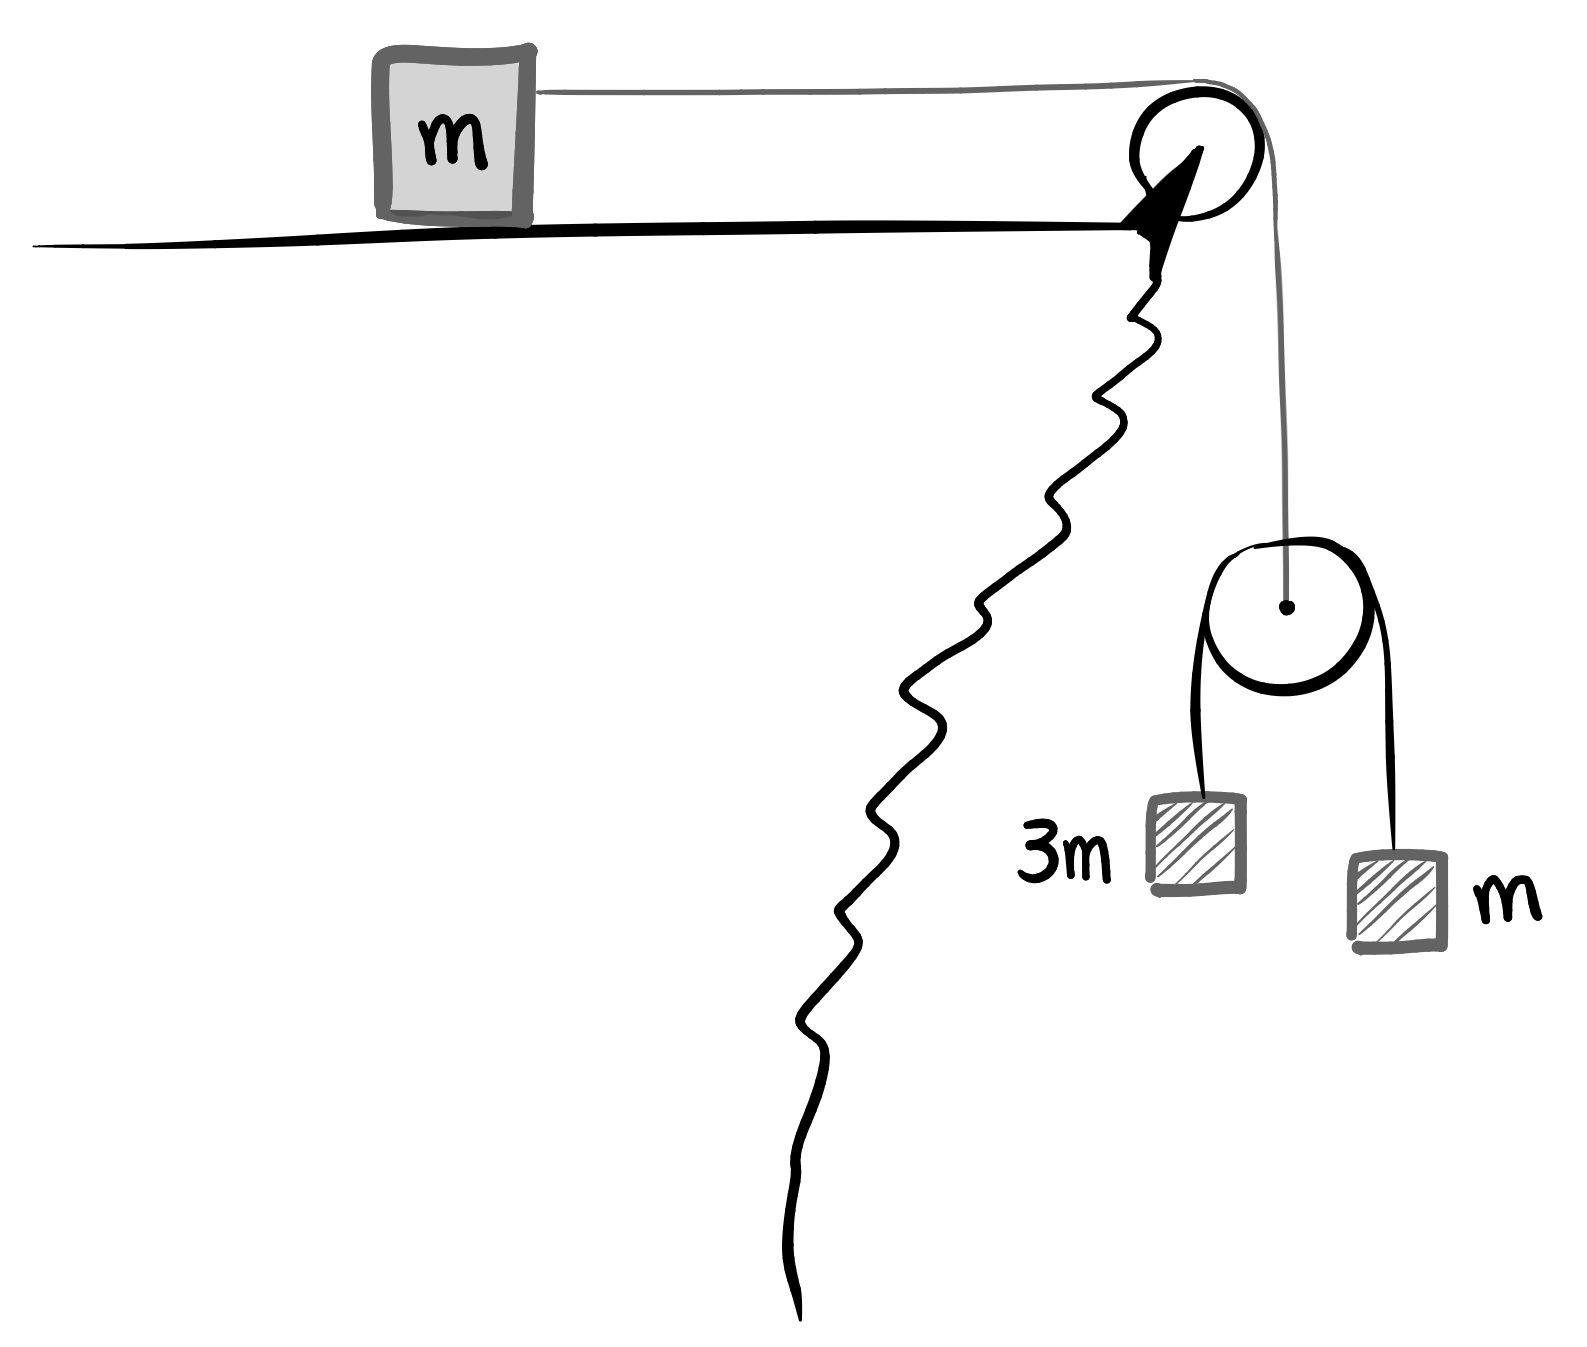
\includegraphics[width=0.4\linewidth]{imagensdinamicanewton/polia movel ex 02.png}};
  \end{scope}
\end{tikzpicture}
\captionof{figure}{}
\label{fig_mec_poliamovelexemplo222a}
} 
\vspace{0.3cm}



\resolucao

Chamemos de bloco $1$ aquele de massa $m$ que está apoiado no solo horizontal. Ele se moverá com aceleração horizontal $a_1=a$ para a direita, como mostra a primeira imagem da Figura \ref{fig_mec_poliamovelexemplo2avancao2}. Com isso, imagine que o sistema dos outros dois blocos estivesse dentro de um elevador: este elevador irá cair verticalmente com a mesma aceleração $a_1$ do bloco horizontal, uma vez que esses dois corpos estão acoplados pelo mesmo fio e devem se mover com a mesma aceleração.


\vspace{0.3cm}
{
\centering
\begin{tikzpicture}
  \begin{scope}[blend mode=multiply]
    \node {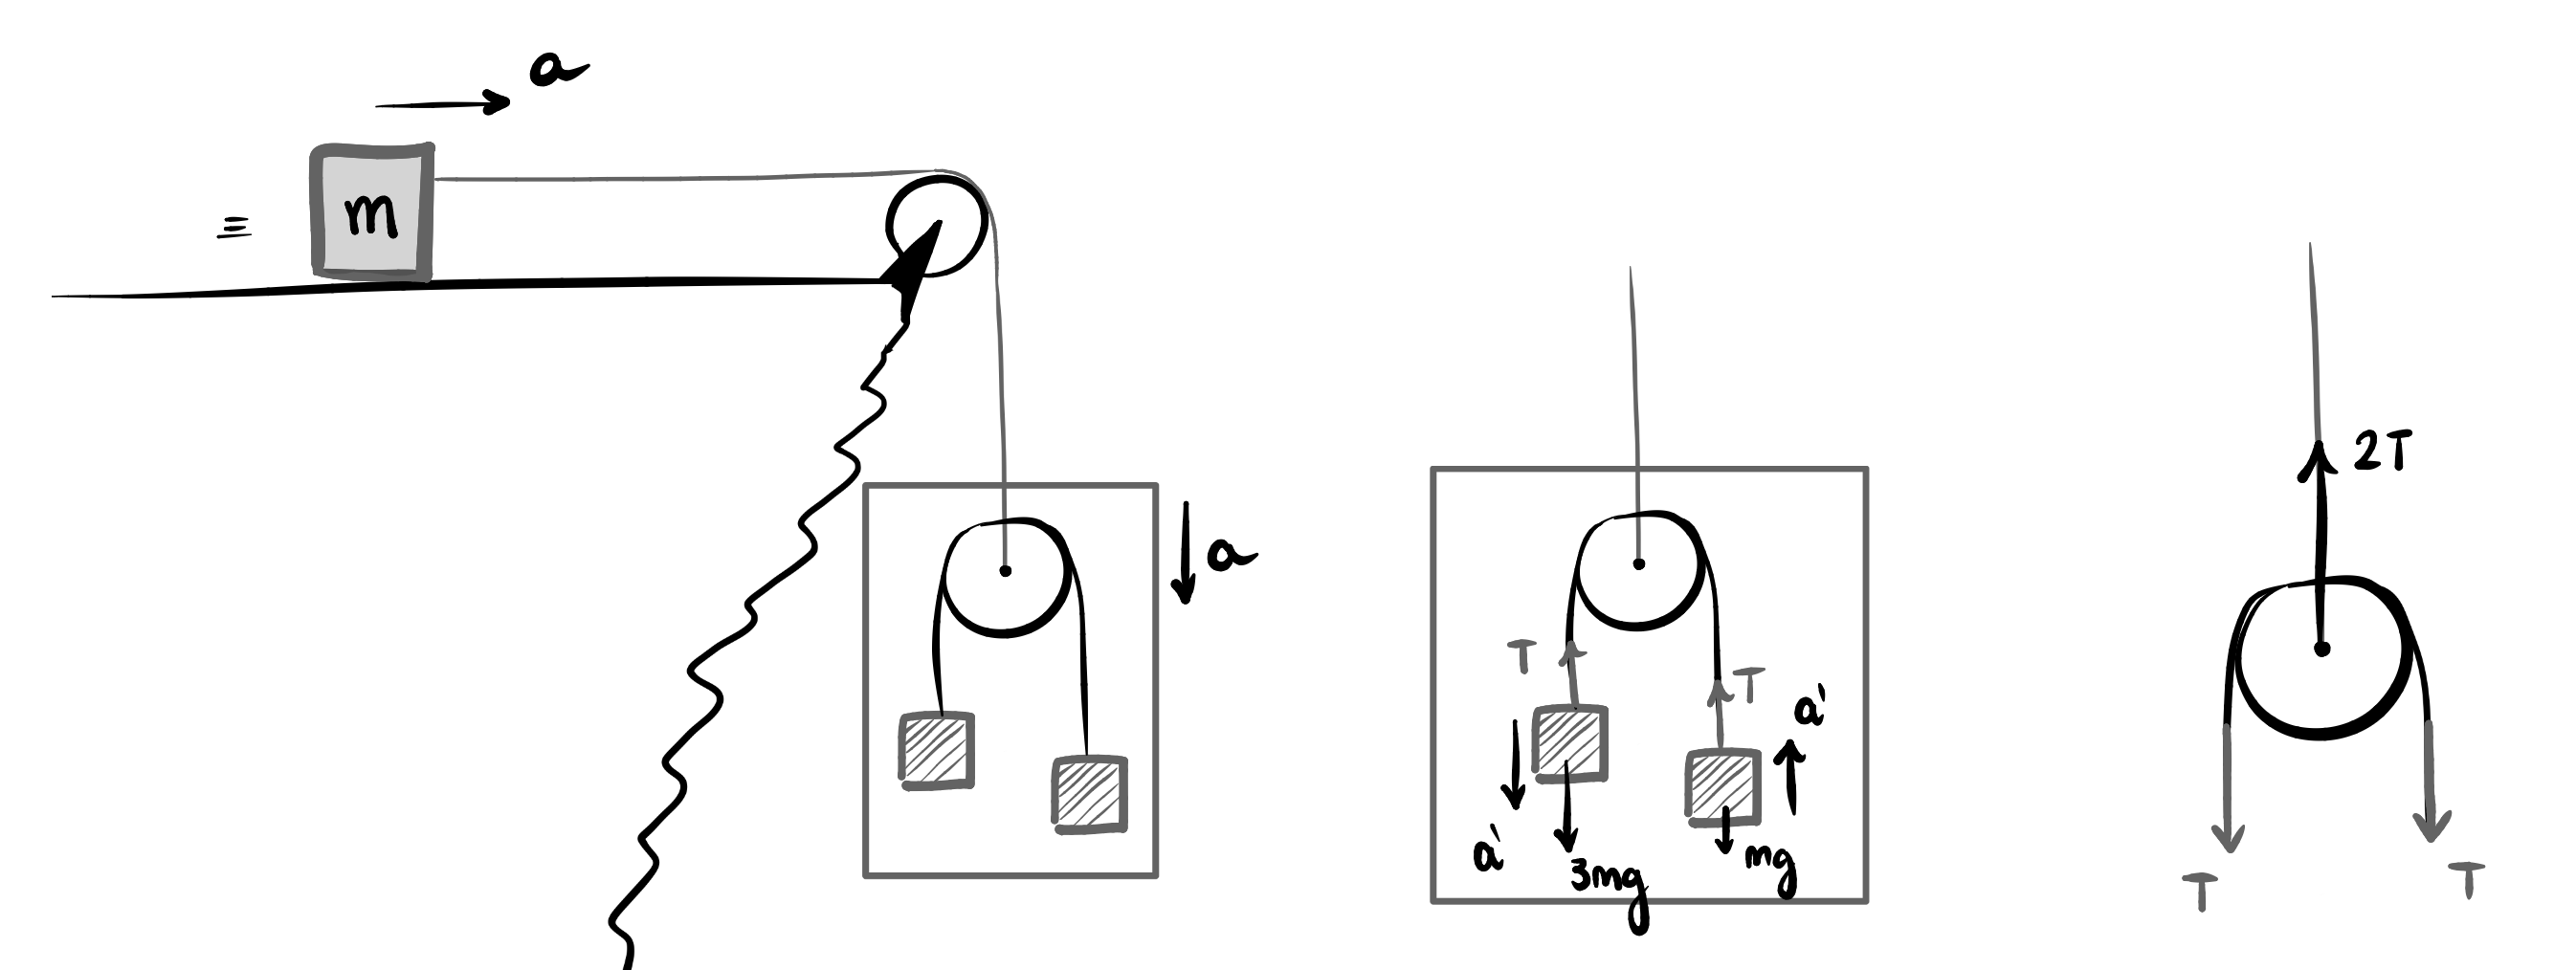
\includegraphics[width=0.9\linewidth]{imagensdinamicanewton/poliamovelexemplo2avancao.png}};
  \end{scope}
\end{tikzpicture}
\captionof{figure}{}
\label{fig_mec_poliamovelexemplo2avancao2}
} 
\vspace{0.3cm}

Contudo, internamente dentro deste elevador, os dois blocos também se movem em movimentos acelerados. Designemos por $a'$ a aceleração destes blocos em relação ao elevador. Logo, as acelerações $a_2$ e $a_3$ dos blocos de massa $3m$ e $m$, internos ao elevador, serão, em relação à Terra, respectivamente iguais a:

\begin{align}
    a_2 &= a_1 + a'  \nonumber \\
    a_3 &= a_1 - a'  \nonumber
\end{align}

Desse modo, a Segunda Lei de Newton para cada um desses blocos diz que

\begin{align}
    3mg - T &= 3 m (a_1 + a') \nonumber \\
    mg-T &=  m (a_1 - a'), \nonumber
\end{align}

\noindent que, subtraindo, nos leva a\footnote{Note que, para o bloco $3$, de massa $m,$ a força resultante foi equacionada para baixo: a força peso menos a tração. Isso foi feito porque partimos da premissa de que sua aceleração total em relação à Terra é para baixo, isto é, ela é $a_3=a_1-a',$ em que $a_1>a'.$}

$$ a_1+2a' = g \quad \text{ e } \quad T = \dfrac{3m(g-a_1)}{2}.$$

A segunda última imagem da Figura \ref{fig_mec_poliamovelexemplo2avancao2} mostra o diagrama de forças na polia móvel: como em toda polia ideal é preciso ter $F_\text{R}=0,$ a tração no fio superior que conecta a polia movel ao bloco horizontal deve ser $2T = 3mg.$ Logo, a Segunda Lei de Newton para o bloco $1$ que está no plano horizontal se escreve como

$$ F_\text{R} = ma \implies 2T = ma_1 \implies  3m(g-a_1) = ma_1 \implies \boxed{a_1 = \dfrac{3g}{4} .}$$

De $a_1+2a' = g$ segue que $a'= g/8,$ de onde segue que

\begin{align}
    a_2 &= a_1 + a' = \dfrac{3g}{4} + \dfrac{g}{8} \implies \boxed{ a_2 = \dfrac{7g}{8}.} \nonumber \\
    a_3 &= a_1 - a' =\dfrac{3g}{4} - \dfrac{g}{8} \implies \boxed{ a_3 = \dfrac{5g}{8}.} \nonumber
\end{align}


A dificuldade dessa questão reside em perceber que todas as acelerações devem ser escritas em relação à Terra para poder equacionar a Segunda Lei de Newton.

\end{exemplo}
\vspace{0.3cm}





% \begin{exemplo}[Nível III]\label{exemplo_newton_poliamovel03}

% Considere os sistemas da Figura \ref{fig_mec_poliamovelexemplo3} com fios e polias ideais, e o valor da gravidade local sendo igual a $g,$ verticalmente para baixo.

% {
% \centering
% 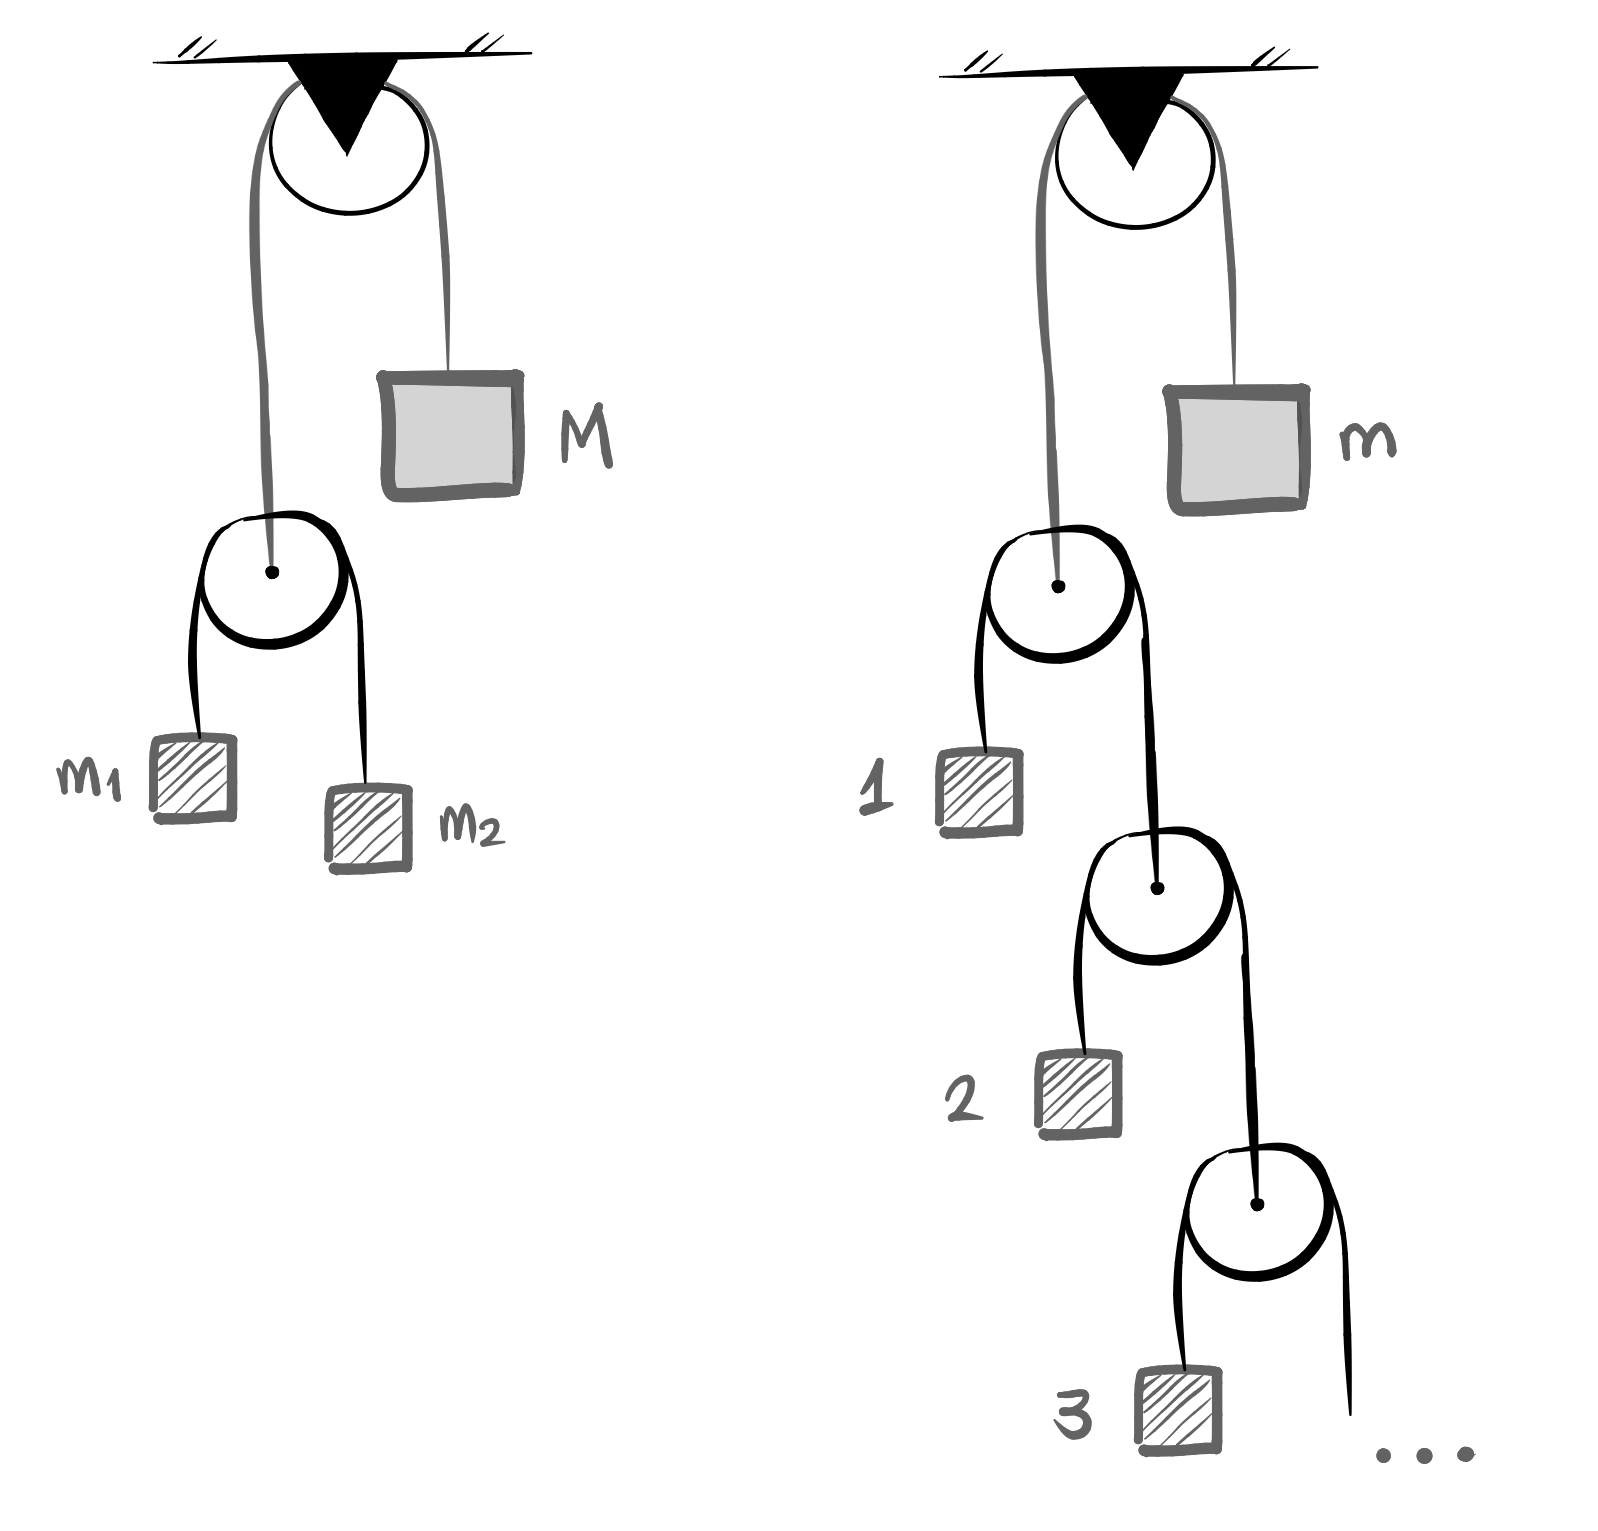
\includegraphics[width=0.5\linewidth]{imagensdinamicanewton/poliamovelex03.png}
% \captionof{figure}{}
% \label{fig_mec_poliamovelexemplo3}
% } 

% \begin{enumerate}


% \item [a)] Considere a máquina de Atwood da primeira imagem da Figura \ref{fig_mec_poliamovelexemplo3}. Qual é o valor de massa $M$, em função de $m_1$ e $m_2,$ que mantêm o sistema em equilíbrio?

% \item [b)] Considere a máquina de Atwood infinita da segunda imagem da Figura \ref{fig_mec_poliamovelexemplo3}. Encontre a tração no fio que prende a polia fixa ao teto, dado que todas as caixas $1,2,3,...$ possuem massa $m.$

% \item [c)] Considere a máquina de Atwood infinita da segunda imagem da Figura \ref{fig_mec_poliamovelexemplo3}. Encontre a tração no fio que prende a polia fixa ao teto, dado que as massas das caixas caem pela metade a cada nova polia, ou seja, $m_1= \sfrac{m}{2}, m_2= \sfrac{m}{4}, m_3= \sfrac{m}{8}, \dots$

% \end{enumerate}
% \resolucao

% 181, 182 e 183 RB

% \end{exemplo}


% \vspace{0.3cm}




\begin{secnivel}[Força de Atrito Estático Máximo]{I}{Força de Atrito Estático Máximo}
  
  \eqLdois{exp}{eq_newton_fatestatico}{F_{\text{AT}_{\text{MAX}}}= \mu_{e} N}

\end{secnivel}







\secgfe{De onde vem}

A Equação \eqref{eq_newton_fatestatico} calcula o valor da força de atrito estático máximo. Antes de examiná-la com mais atenção, convém compreender a natureza da força de atrito de maneira mais ampla.

Primeiro, vamos discorrer sobre sua origem. A força de atrito entre duas superfícies é uma força que irá resistir à tendência de movimento relativo entre as superfícies pelo fato de elas estarem, em escala microscópica, ``\textit{acopladas}.'' A Figura \ref{fig_mec_fatorigem} mostra essa situação, em que temos um bloco em equilíbrio em cima do solo. Ao observarmos a superfície de contato entre o bloco e o solo vemos que, diferente do que enxergamos a olho nu, tal superfície é repleta de irregularidades. 


\vspace{0.3cm}
{
\centering
\begin{tikzpicture}
  \begin{scope}[blend mode=multiply]
    \node {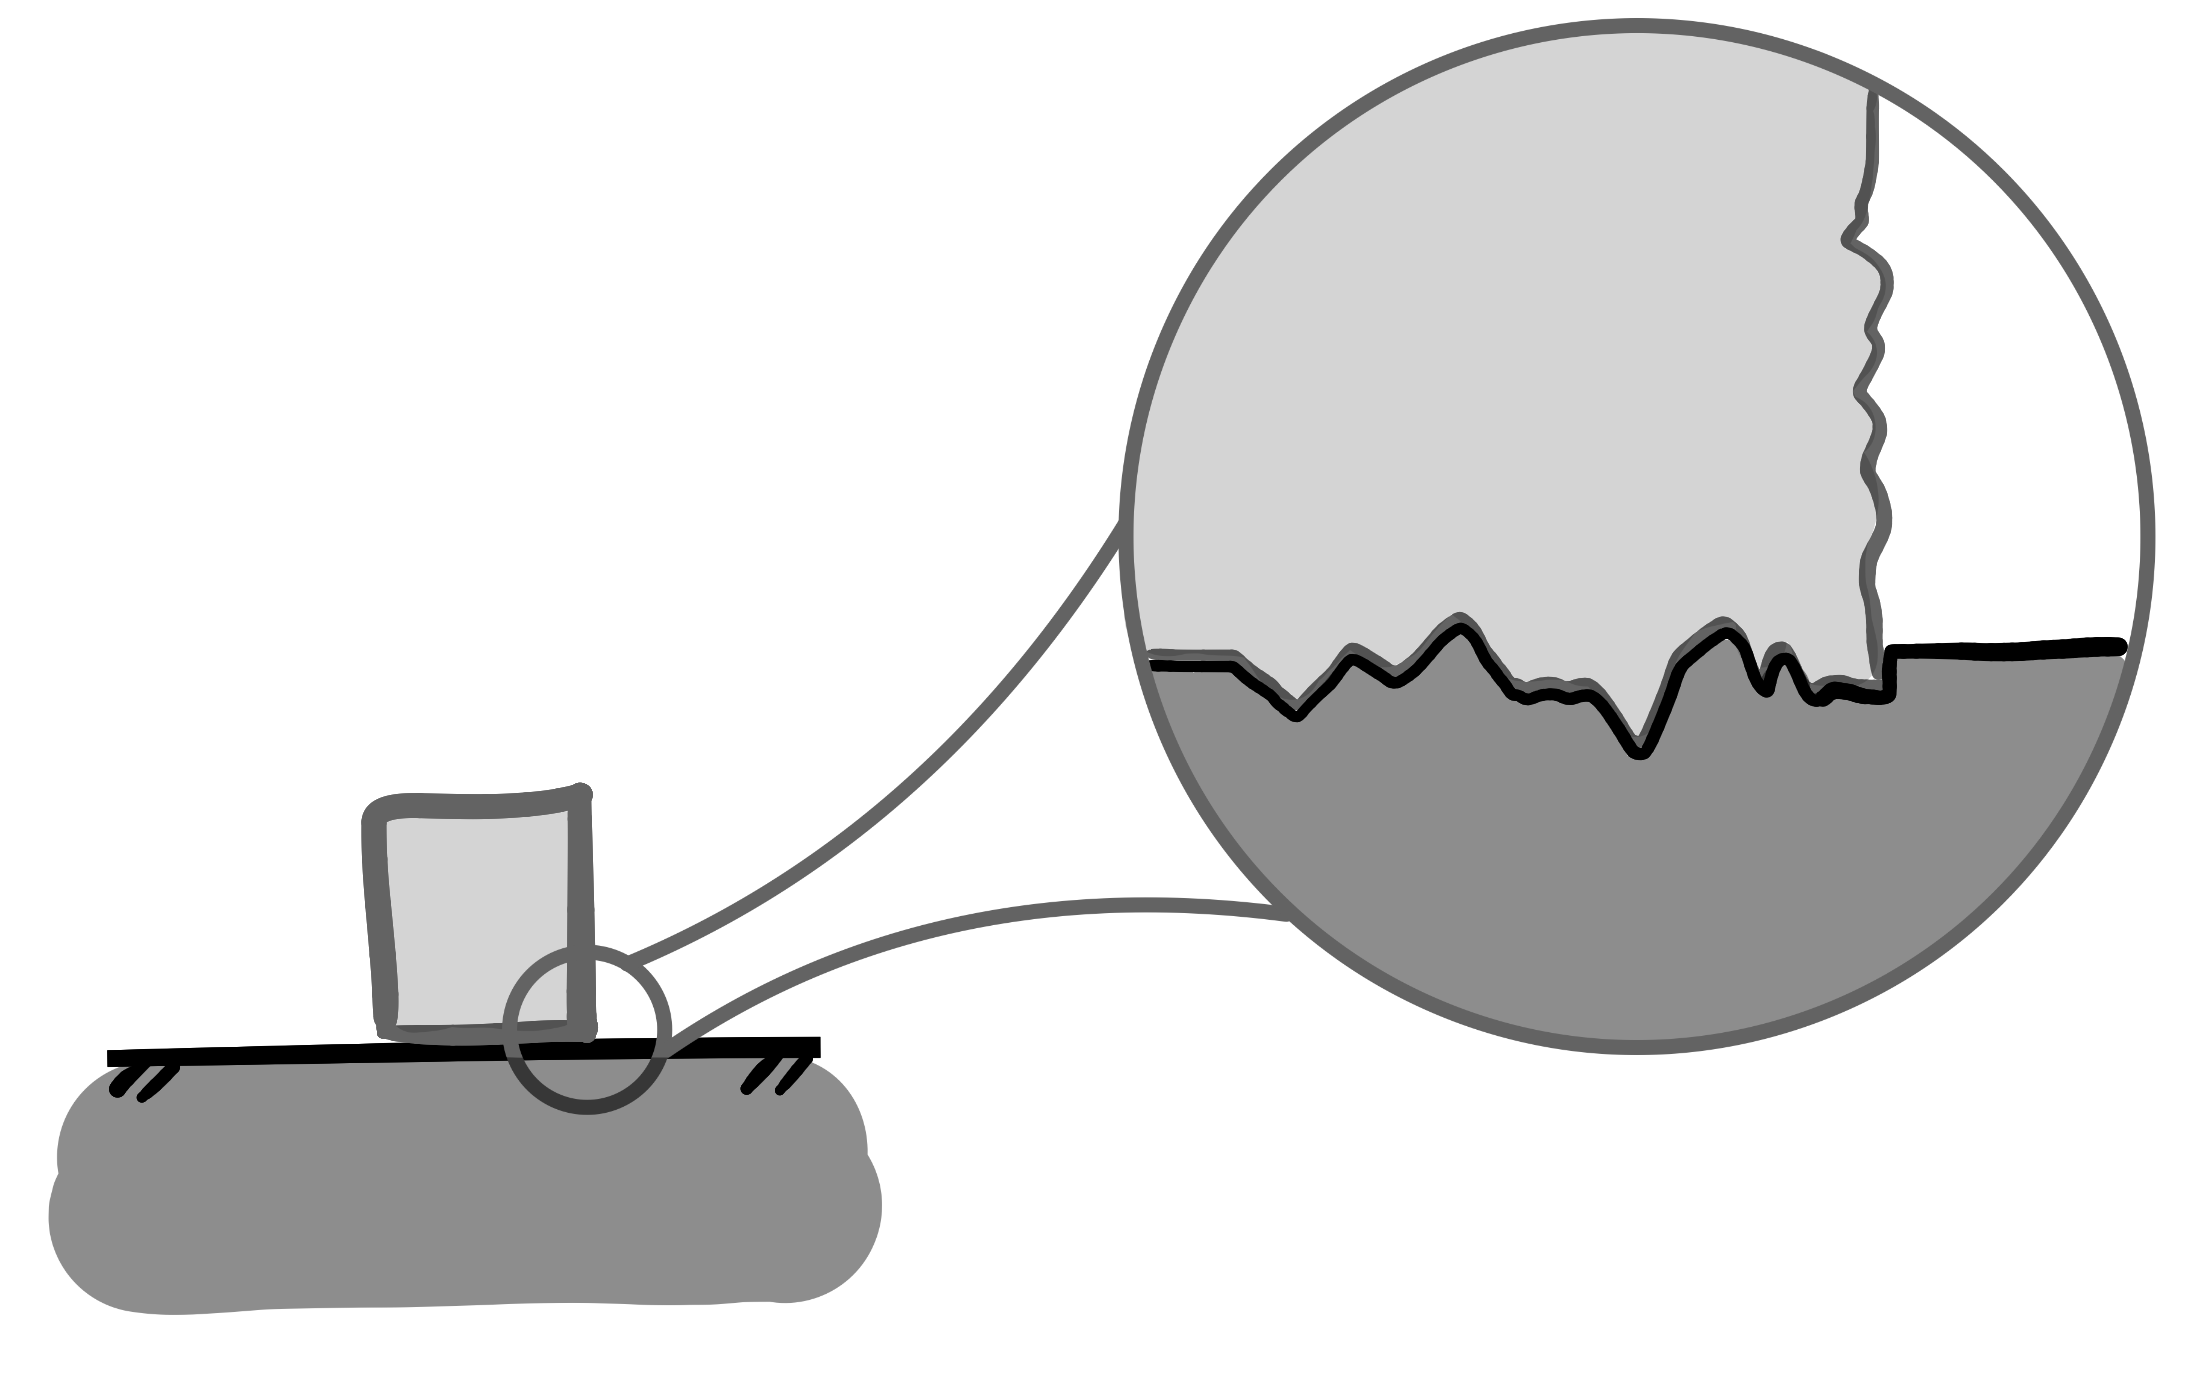
\includegraphics[width=0.4\linewidth]{imagensdinamicanewton/fatorigem.png}};
  \end{scope}
\end{tikzpicture}
\captionof{figure}{A origem da força de atrito.}
\label{fig_mec_fatorigem}
} 
\vspace{0.3cm}

Tais irregularidades se interpenetram, fazendo com que o bloco fique, de certo modo, fincado no solo, como se fossem raízes de um árvore. Assim, ao tentar movê-lo, encontraremos certa resistência para tal movimento. Essa resistência não existiria caso as superfícies fossem totalmente lisas, sem nenhuma irregularidade. Por isso, polir e lixar uma superfície (que é um tentativa de eliminar as irregularidades e deixá-la mais lisa) é uma forma de diminuir o atrito.




Em segundo lugar, sendo o atrito uma força, sabemos que se trata de uma grandeza vetorial, que possui, portanto, módulo, direção e sentido. Tratemos agora da sua direção e sentido. Estando a superfície do bloco da Figura \ref{fig_mec_fatorigem} ``\textit{fincada}'' no chão, é natural perceber que a força de atrito que se manifestará será paralela a tal superfície de contato; isto é, ela será, nesse caso, horizontal.

Isso porque, ao tentar empurrar o bloco, digamos, para a direita, as saliências e irregularidades do bloco penetradas na superfície do solo irão empurrar o solo para a direita. Assim, o solo reage e faz uma força para a esquerda no bloco. As forças trocadas, portanto, possuem sempre a direção da superfície de contato (sempre paralela ao plano, podendo ser para a direita ou para a esquerda).

Agora que já sabemos sobre a direção da força de atrito, vamos ao seu sentido: ela é sempre contrária à \textbf{tendência de movimento}. Essa é uma nuance que costuma gerar muitos erros. Note que ela exige um certo nível de abstração, uma vez que o bloco pode sequer se mover: é preciso imaginar, dadas as forças aplicadas nele, para onde ele \textbf{tende a se mover.} No caso de empurrar para a direita o bloco da Figura \ref{fig_mec_fatorigem}, a tendência é que ele se mova para a direita. Logo, o atrito, contrariando essa tendência, atua no bloco para a esquerda (isso se dá pela Terceira Lei de Newton, como construímos no raciocínio do parágrafo anterior). Perceba que, ao empurrar o bloco para a direita, pode ser que ele continue parado. Ou seja, ele sequer se move: o atrito estático é suficiente para mantê-lo em repouso e seria necessária uma força maior para colocá-lo em movimento. Sendo assim, é preciso sempre estar atento à tendência de movimento. O movimento em si pouco importa -- pode ser que ele sequer ocorra.

Na Figura \ref{fig_mec_fatcontratendenciamov} ilustramos diversos casos para que o leitor se familiarize com tal conceito. O primeiro caso é exatamente aquele da Figura \ref{fig_mec_fatorigem}, então dispensaremos sua análise. 

No segundo caso, ao empurrar o bloco de baixo pra direita com uma força $F$, sua tendência é se mover para a direita, naturalmente. Logo, o bloco de cima, por inércia, tende a ficar parado. Contudo, ficar parado em relação a um corpo que se move para a direita significa ficar para trás em relação a ele, ou seja, escorregar para a esquerda. Como a tendência do bloco de cima é escorregar para a esquerda em relação ao bloco de baixo, a força de atrito entre os blocos,\footnote{Analisamos aqui só as forças de atrito entre os blocos. Poderia haver também atrito entre o bloco maior e o chão. Neste caso, seria a mesma situação da primeira imagem da figura: o atrito atuaria para a esquerda.} contrariando tal tendência de movimento, atua para a direita, como mostra a imagem.

Na terceira situação da Figura \ref{fig_mec_fatcontratendenciamov} colocamos um bloco sob um plano inclinado, em repouso. Sua tendência, naturalmente, é escorregar plano abaixo. Logo, o atrito, contrário à tendência de movimento, atua na direção do plano, apontando para cima.

\vspace{0.3cm}
{
\centering
\begin{tikzpicture}
  \begin{scope}[blend mode=multiply]
    \node {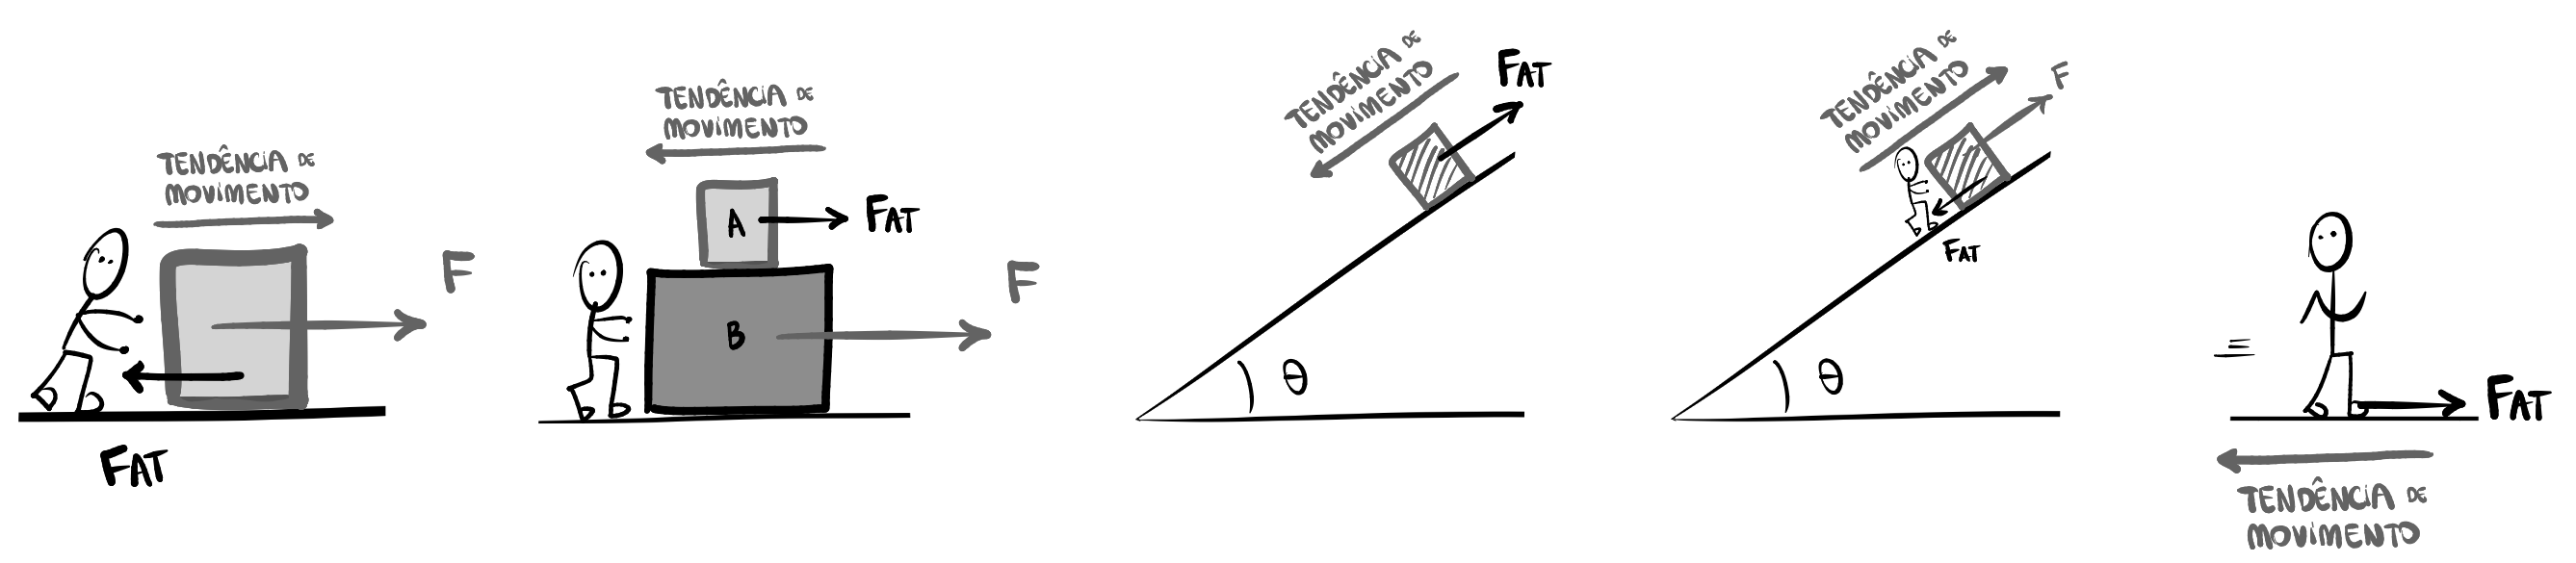
\includegraphics[width=1.0\linewidth]{imagensdinamicanewton/fatcontratendenciamov.png}};
  \end{scope}
\end{tikzpicture}
\captionof{figure}{A força de atrito é sempre paralela à superfície de contato entre os corpos e sempre se opõe à tendência de movimento.}
\label{fig_mec_fatcontratendenciamov}
} 
\vspace{0.3cm}

Já a quarta situação ilustra um contexto semelhante, porém agora um menino está empurrando o bloco com uma força tal que ele está quase começando a se mover plano acima. Assim, identificamos que a tendência de movimento do bloco é subir plano acima e o atrito, portanto, ao contrariar tal tendência de movimento, atua plano abaixo. Veja que curioso: na mesma situação -- um bloco sob um plano inclinado -- o atrito pode atuar plano acima ou plano abaixo. Tudo irá depender de qual é a tendência de movimento do bloco.

A última situação ilustra um exemplo cotidiano: o ato de andar. Ao dar um passo, fazemos um movimento de ``empurrar o chão para trás.'' A tendência, portanto, é que nosso pé escorregue para trás\footnote{Faça esse movimento sob uma casca de banana ou uma pista de gelo e constate por si só}, logo, o atrito, contrariando a tendência de movimento, atua para frente. Perceba, portanto, que neste caso o atrito atua a favor do movimento. Alguns leitores podem se surpreender com isso em um primeiro problema, mas não há nada de estranho: a força de atrito sempre se opõe à tendência de movimento, e não ao movimento em si. Portanto, não há nada de incoerente em uma situação na qual o atrito atue na mesma direção e sentido que o movimento -- veremos diversas situações como essa, inclusive.\footnote{Com isso, destaca-se que o atrito, portanto, pode tanto acelerar quanto desacelerar um corpo.}

Neste último caso, é o atrito que possibilita que o indivíduo caminhe, e é por isso que em uma superfície com pouco atrito (como uma pista de gelo) é muito difícil caminhar.




Em terceiro e último lugar, tratemos sobre o módulo da força de atrito. É exatamente isso que a Equação \eqref{eq_newton_fatestatico} se propõe a calcular. Na verdade ela se propõe a calcular o módulo da força de atrito estático \textbf{máximo}. Como veremos em breve, a força de atrito estático possui módulo variável, admitindo um valor máximo, que é aquele dado pela Equação \eqref{eq_newton_fatestatico}.

Tal equação é obtida por meio de experimentos, mas podemos compreendê-la com facilidade à luz de alguns conceitos que já construímos. Lembre-se da origem da força de atrito: ela está relacionada às irregularidades e rugosidades dos materiais, que fazem com eles fiquem ``fincados'' um no outro. Ora, quanto mais comprimido o bloco da Figura \ref{fig_mec_fatorigem} estiver contra o solo, mais ``fincado'' no solo ele estará e, consequentemente, maior será a força de atrito. Aqui, lembramos o leitor quem é o ente responsável por medir o quão comprimidas duas superfícies estão uma contra a outra: a força normal. 

A força normal é justamente definida como sendo a força de compressão entre duas superfícies em contato, sendo perpendicular a tal superfície de contato. Logo, é por isso que ela aparece na Equação \eqref{eq_newton_fatestatico}: a força de atrito é diretamente proporcional à compressão entre as superfícies: a força normal.

O termo $\mu_e$ é o chamado coeficiente de atrito estático, e é o termo que está relacionado ao quanto às superfícies em questão conseguem se acoplar. Trata-se de uma grandeza adimensional, em geral com valor entre 0 e 1, e é um valor obtido experimentalmente.

Digamos, por exemplo, que, por meio de experimentos, identifica-se que o coeficiente de atrito estático entre a madeira e o concreto é $\mu_e = 0.6.$ Se polirmos bem tais superfícies e, quem sabe, a lubrificarmos, conseguiremos diminuir o atrito, de modo que o coeficiente de atrito estático agora seria, digamos, $\mu_e = 0.3.$ Perceba, portanto, que tal coeficiente mede o quão bem as duas superfícies irão se acoplar: se polirmos as superfícies e diminuirmos suas irregularidades, o coeficiente de atrito diminui. Na chuva, como a estrada fica mais escorregadia, o coeficiente de atrito entre os pneus e o asfalto é menor do que no caso em que o asfalto está seco, por isso a estrada fica mais perigosa.


\secgfe{Onde é usada}

Como a Equação \eqref{eq_newton_fatestatico} calcula o valor da força de atrito estático máximo, isto é, o maior valor que a força de atrito pode assumir, ela é usada em geral em problemas nos quais um corpo se encontra na \textbf{iminência de se mover.} Ou seja, o corpo está sendo segurado pela força de atrito, mas está quase rompendo sua situação de equilíbrio: isso quer dizer que o atrito estático está assumindo o maior valor que pode. Daí em e diante ele não será capaz de segurar mais o bloco em equilíbrio.

\vspace{0.3cm}
{
\centering
\begin{tikzpicture}
  \begin{scope}[blend mode=multiply]
    \node {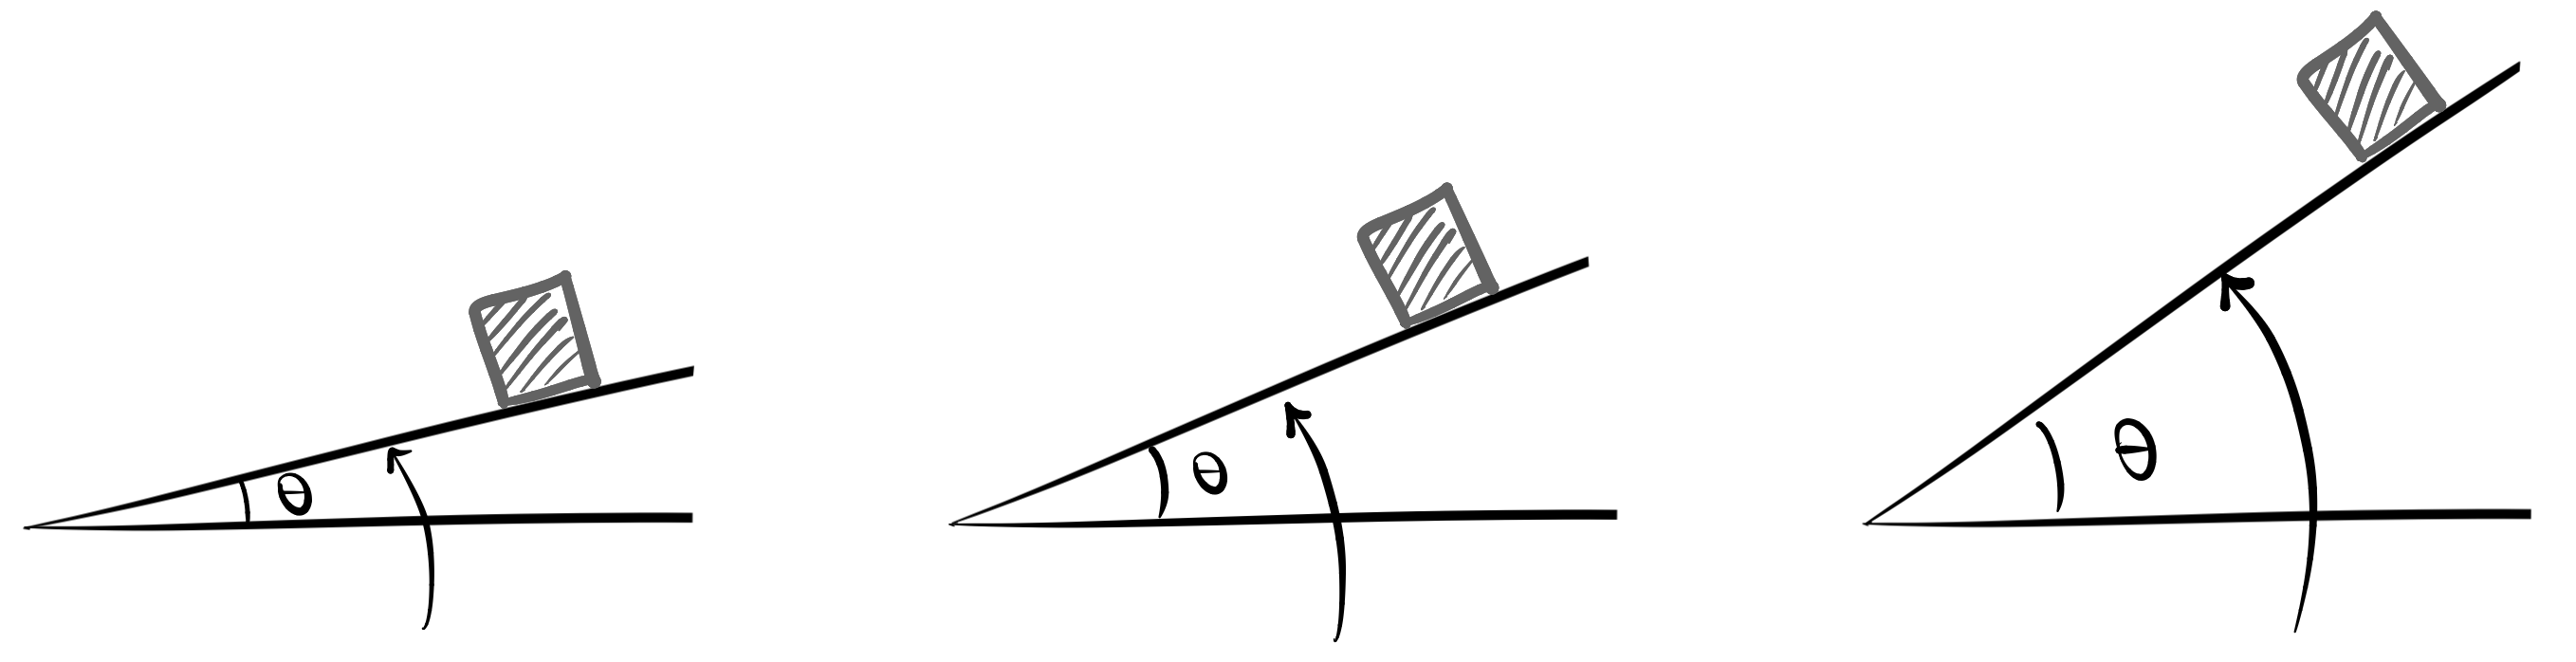
\includegraphics[width=0.8\linewidth]{imagensdinamicanewton/angulodeatrito1.png}};
  \end{scope}
\end{tikzpicture}
\captionof{figure}{}
\label{fig_mec_anguloatrito01}
} 

Para ilustrar isso, considere o experimento da Figura \ref{fig_mec_anguloatrito01}, em que um bloco está em equilíbrio sob um plano inclinado. O experimento consiste em ir aumentando gradativamente a inclinação do plano, até que o bloco se encontre na iminência de escorregar. Neste ponto, teremos inclinado tanto o plano de modo que o atrito está no seu limite: ele quase não consegue mais segurar o bloco em repouso. Essa é a situação em que a força de atrito estático assume seu valor máximo, que é justamente o contexto da Equação \eqref{eq_newton_fatestatico}.

\vspace{0.3cm}
{
\centering
\begin{tikzpicture}
  \begin{scope}[blend mode=multiply]
    \node {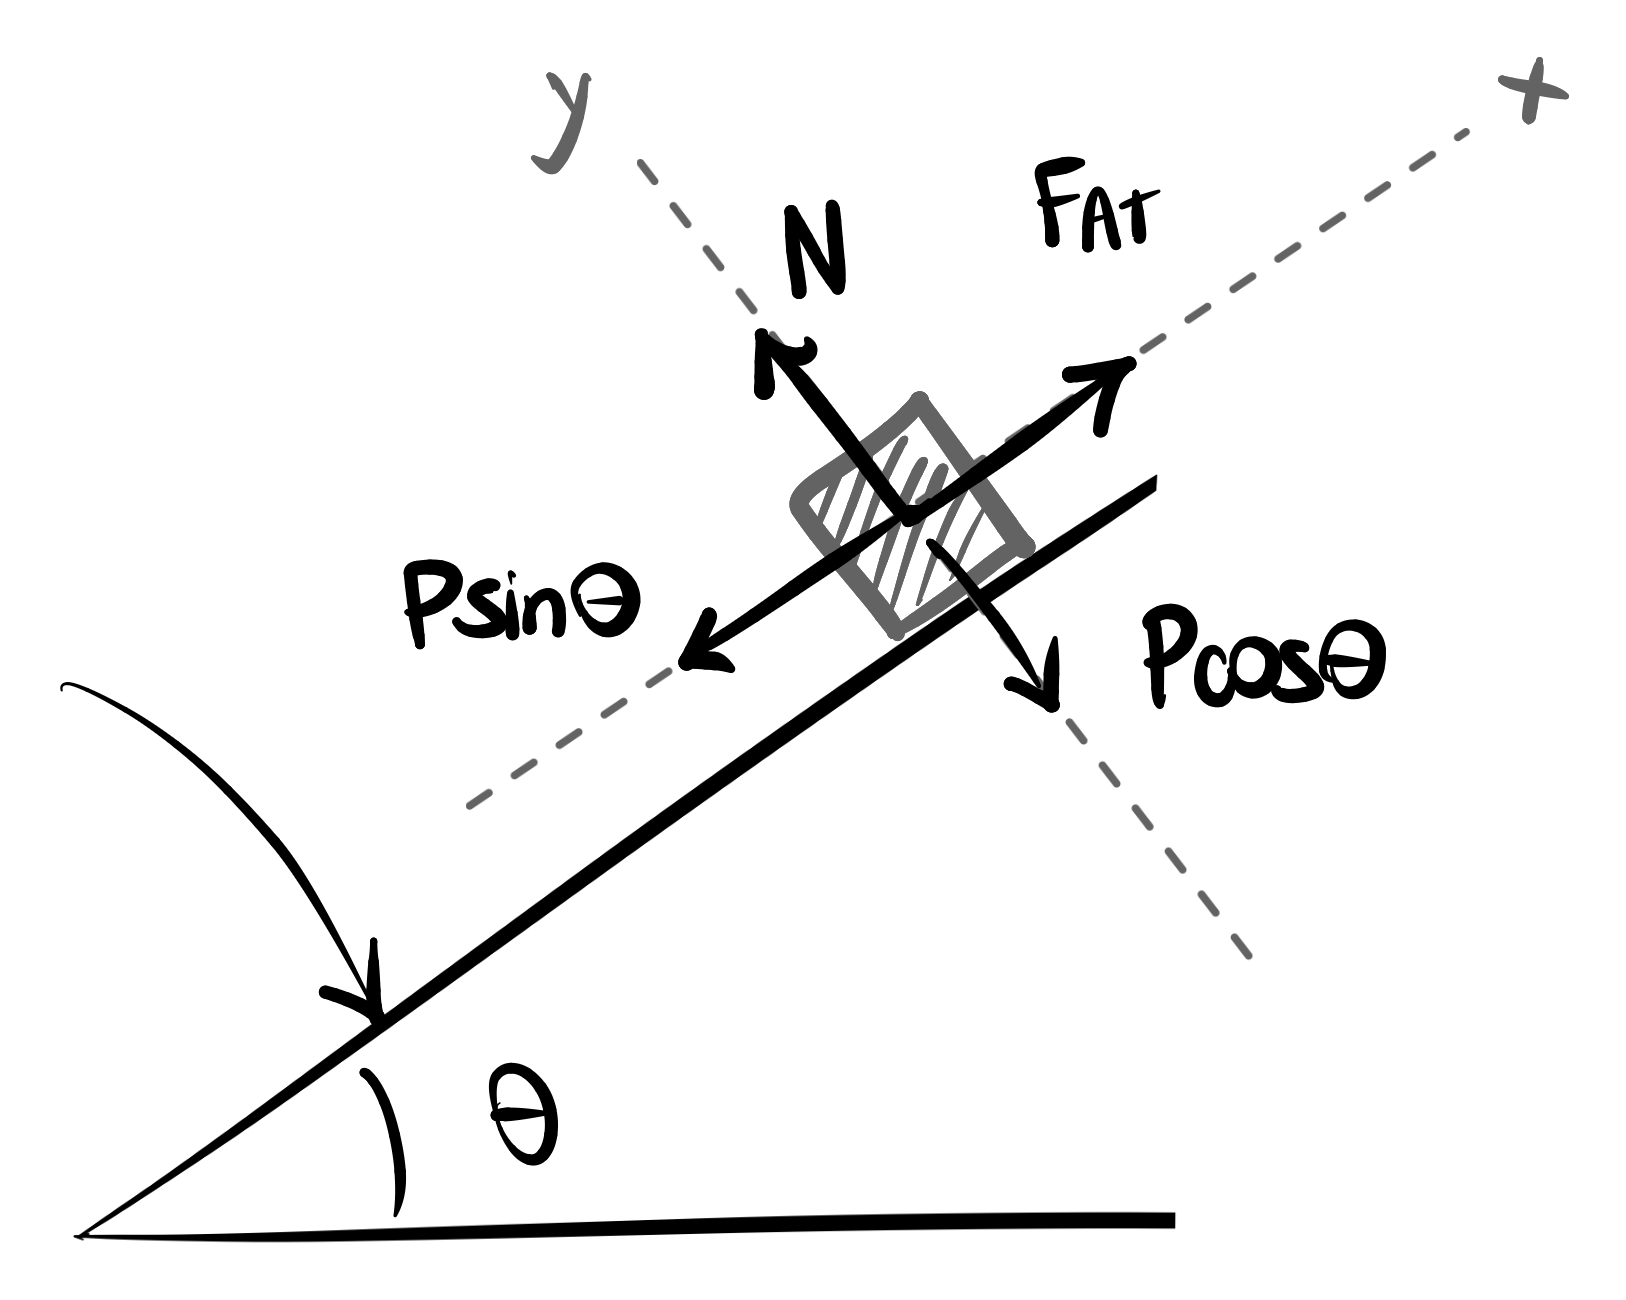
\includegraphics[width=0.3\linewidth]{imagensdinamicanewton/angulodeatrito2.png}};
  \end{scope}
\end{tikzpicture}
\captionof{figure}{}
\label{fig_mec_anguloatrito02}
} 
\vspace{0.3cm}

Essa situação está representada na última imagem da figura. O diagrama de forças de tal situação está representado na Figura \ref{fig_mec_anguloatrito02}, em que a força peso já foi representada decomposta nos eixos tangencial e normal, exatamente como feito para construir a Equação \eqref{eq_dinamicanewtoniana_gsintheta}. Do equilíbrio do bloco temos:


 \[
 \vec{F}_R = 0
\quad \xrightarrow{\text{projeção nos eixos}}
\quad
\begin{cases}
F_x = 0 \implies P \sin \theta = F_{\text{AT}_{\text{MAX}}} \\
F_y = 0 \implies P \cos \theta = N
\end{cases}
\] 

Usando a Equação \eqref{eq_newton_fatestatico} e as duas relações acima teremos:

$$ F_{\text{AT}_{\text{MAX}}} = \mu_e N \implies P \sin \theta = \mu_e P \cos \theta \implies \boxed{\mu_e = \tan \theta.} $$

O ângulo $\theta$ dado pela expressão acima é chamado de \textbf{ângulo de atrito:} sua tangente fornece justamente o coeficiente de atrito entre as superfícies do plano e do bloco.



Tal experimento é usado justamente para se determinar o coeficiente de atrito estático entre duas dadas superfícies. Por meio do cálculo da tangente do ângulo de atrito -- e o ângulo de inclinação do plano que deixa o bloco na iminência de movimento -- obtém-se o coeficiente de atrito estático.

\secgfe{Erros comuns}

O erro mais comum ao usar a Equação \eqref{eq_newton_fatestatico} é na sua interpretação: tal equação não fornece o valor da força de atrito estático, mas sim o da \textbf{força de atrito estático máximo.} Observe a Figura \ref{fig_mec_fatestaticovariavel} para entender essa diferença. 

Ao tentar empurrar o bloco, o menino começa fazendo uma força horizontal $F=20$N. Ele constata que o bloco, que estava inicialmente parado, permanece parado. Logo, a resultante das forças que nele atua permanece sendo nula, de onde conclui-se que o atrito estático respondeu com uma força cujo módulo vale, também, $20$N. 

Ao aumentar a força do empurrão para tentar tirar o bloco do lugar o menino faz uma força de $50$N, tão logo isso acontece ele constata que tal esforço foi insuficiente: o bloco continua em equilíbrio estático. Logo, conclui-se que o atrito estático respondeu com uma força cujo módulo vale, também, $50$N. E por aí vaí: ao empurrar o bloco com uma força de 55N o atrito responde com 55N, mantendo o bloco em repouso. Isso ocorre para diversos valores de força: o atrito sempre consegue igualar a força feita pelo menino, mantendo o bloco em repouso. Quer dizer, isso ocorre...até certo ponto.


\vspace{0.3cm}
{
\centering
\begin{tikzpicture}
  \begin{scope}[blend mode=multiply]
    \node {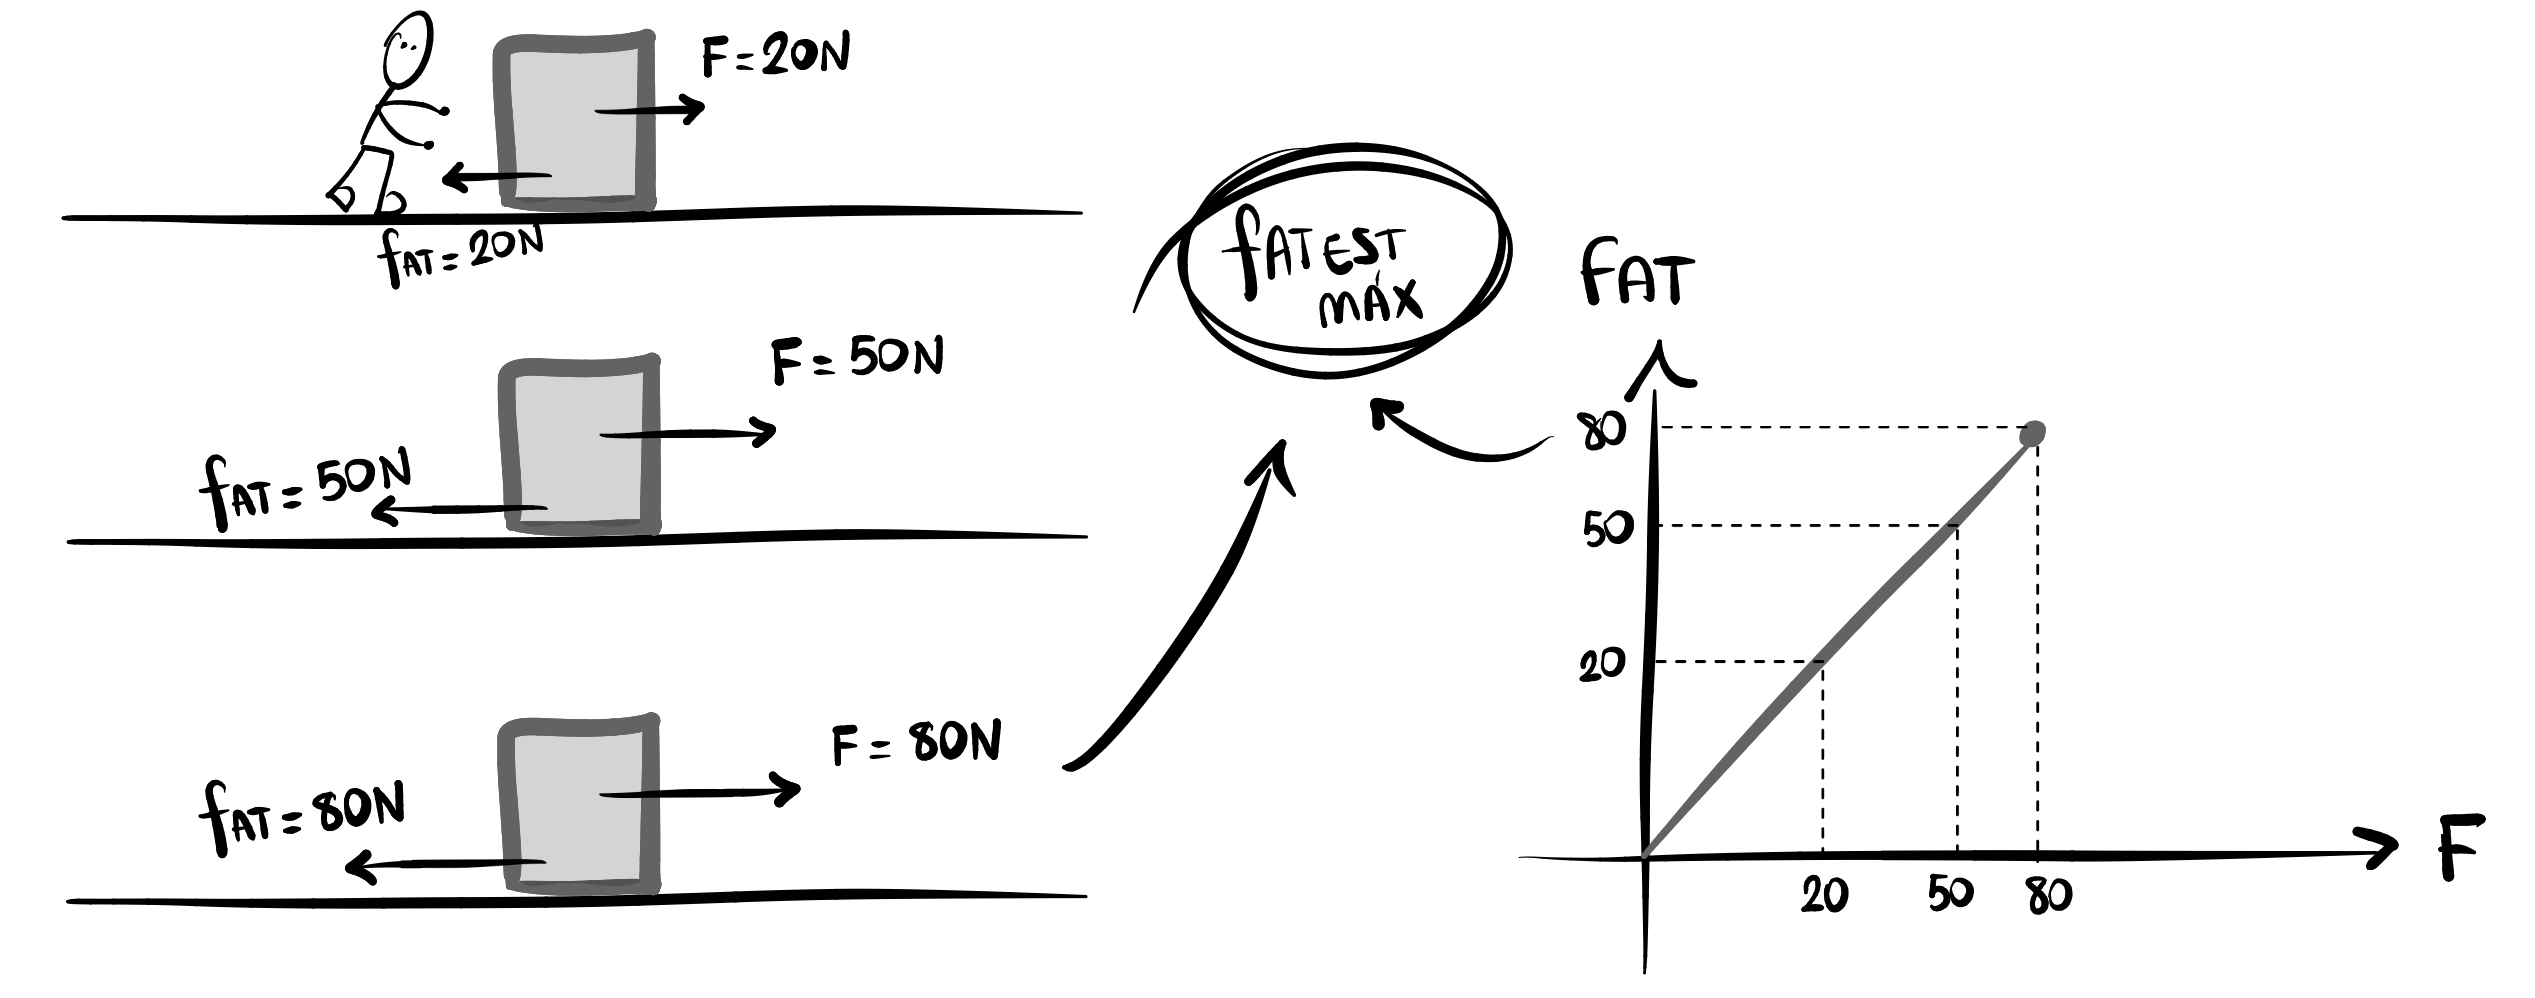
\includegraphics[width=0.8\linewidth]{imagensdinamicanewton/fatestaticovariavel.png}};
  \end{scope}
\end{tikzpicture}
\captionof{figure}{A força de atrito estático possui módulo variável, se igualando à força que a opõe, até um valor máximo.}
\label{fig_mec_fatestaticovariavel}
} 
\vspace{0.3cm}

Ao fazer uma força de $80$N o menino constata que está quase obtendo êxito em sua empreitada: o bloco está quase movendo, mais um cabelímetro\footnote{Um cabelímetro corresponde, aproximadamente, à espessura de um fio de
cabelo humano --- algo em torno de $70\,\mu$m, a depender da hidratação do autor
no dia da medição. Trata-se de uma unidade não reconhecida pelo Sistema Internacional
de Unidades, pelo Bureau Internacional de Pesos e Medidas, nem pela vizinha do autor,
que consultada a respeito manifestou indiferença. Sua principal vantagem em relação
ao micrômetro é fonética: ninguém nunca precisou soletrar cabelímetro duas vezes.} de força deve ser suficiente para tirá-lo do lugar. Essa condição é justamente a de iminência de movimento: o bloco está quase rompendo o equilíbrio estático, o atrito está quase deixando de ser capaz de mantê-lo em repouso. A essa força de atrito damos o nome de \textbf{força de atrito estático máxima,} e é ela que a Equação \eqref{eq_newton_fatestatico} se propõe a calcular.

Perceba, portanto, que a força de atrito estático tem módulo variável, como indica o próprio gráfico da Figura \ref{fig_mec_fatestaticovariavel}, que plota os dados da situação do menino empurrando o bloco. Porém, ela admite um valor máximo -- que corresponde à situação limite em que o repouso entre o bloco e a superfície do chão será mantido. Ao empurrar o bloco com uma força que seja um milésimo maior do que $80$N o bloco romperá seu equilíbrio e começará a se mover: o menino logrou êxito em sua tarefa. 

Daí em diante, ao começar a se mover, o atrito que atuará será o cinético, dado pela Equação \eqref{eq_newton_fatcinetico}, e será estudado na sequência.

Assim, caso o leitor prefira, é possível ler a Equação \eqref{eq_newton_fatestatico} como uma desigualdade: ela impõe um limite superior para a força de atrito estático, isto é:

$$ F_{AT} \leq \mu_{e} N. $$

O gráfico da Figura \ref{fig_mec_fatestaticovariavel} deixa isso evidente: a força de atrito estático pode assumir quaisquer valores, desde que sejam menores (ou igual) a $\mu_e N,$ que é o seu valor máximo.

\secgfe{Observações}

Acredito que cabem duas observações importantes a respeito da Equação \eqref{eq_newton_fatestatico}. A primeira delas é sobre o coeficiente de atrito $\mu_e$:

\begin{enumerate}
    \item ele é uma grandeza adimensional: é uma razão entre duas forças, a força de atrito e a força normal, e, portanto, não possui unidade de medida.

    \item  o coeficiente de atrito não é uma propriedade intrínseca do corpo, é algo que depende das duas superfícies que estão em contato. O coeficiente de atrito entre uma caixa de madeira e uma superfície de metal será, em geral, diferente do coeficiente de atrito entre a mesma caixa de madeira uma superfície de madeira, por exemplo.
\end{enumerate}


A segunda observação é sobre o movimento relativo. Ao ler a Equação \eqref{eq_newton_fatestatico}, por se tratar do atrito estático, o leitor pode ser levado a crer que tal equação se aplica só se o bloco estiver parado. Isso até está correto...contudo, o que significa estar parado? Como vimos na construção da Equação \eqref{mecanica_eq_velocidaderelativa}, um corpo parado em um referencial pode muito bem -- e em geral estará -- estar se movendo em relação a outro.

Dito isso, o termo estático que caracteriza tal atrito está relacionado ao movimento relativo entre as duas superfícies que estão em contato no contexto. Se um bloco está sob uma superfície horizontal, o atrito atuante será estático caso a superfície do bloco não se mova \textbf{em relação ao chão} (ela pode muito bem estar se movendo em relação a algum outro observador). Considere, por exemplo, a situação da Figura \ref{fig_mec_atritoestaticomovendo1}.

\vspace{0.3cm}
{
\centering
\begin{tikzpicture}
  \begin{scope}[blend mode=multiply]
    \node {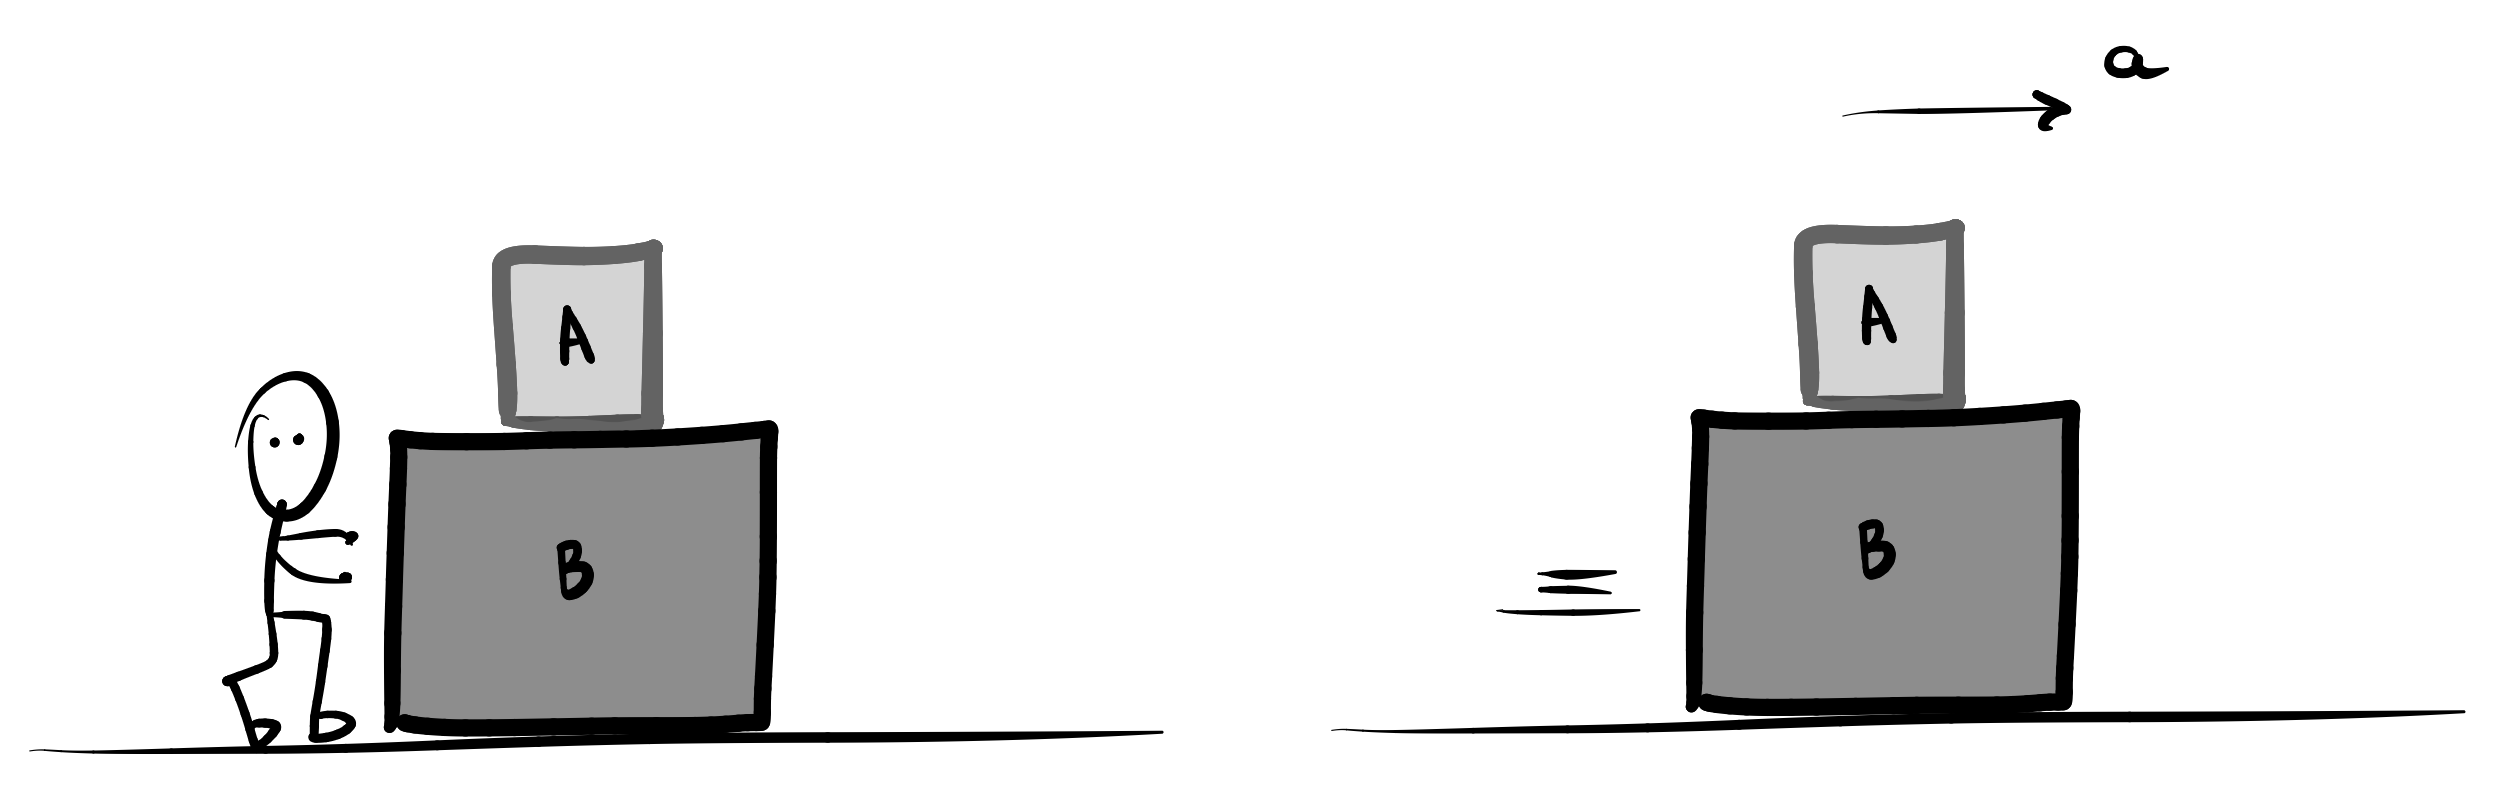
\includegraphics[width=0.7\linewidth]{imagensdinamicanewton/atritoestaticomovendo1.png}};
  \end{scope}
\end{tikzpicture}
\captionof{figure}{Quando os dois blocos aceleram juntos, sem que $A$ escorregue em relação a $B,$ então eles possuem exatamente a mesma aceleração e $A$ está em repouso em relação a B.}
\label{fig_mec_atritoestaticomovendo1}
} 
\vspace{0.3cm}

A situação mostra um pequeno bloco, de massa $m$, apoiado em cima de um outro bloco maior, de massa $M.$ Este, por sua vez, está apoiado no chão. Um indivíduo empurra o bloco de baixo e consegue imprimir uma aceleração $a$ no sistema, que se move de tal sorte que o bloco de cima não se move em relação ao bloco debaixo.

Não seria espantoso que um espírito ainda não calejado na solução de uma grande diversidade de problemas de física imaginasse, com certa confiança prematura, que, como os blocos se movem, o atrito que atua entre eles não poderia ser estático.

Isso certamente está errado pois, como bem lembramos, o adjetivo estático em questão se refere à superfície de contato entre os corpos. Se observarmos bem, o contexto do problema nos diz que os blocos se movem juntos, sem que um escorregue em relação ao outro. Isso quer dizer que eles se movem -- em relação à Terra -- exatamente com a mesma aceleração e, portanto, estão em repouso um em relação ao outro.




Poderíamos, inclusive, computar qual deve ser a máxima aceleração $a$ a se imprimir neste sistema tal que essa situação seja possível. Para isso, considere que o coeficiente de atrito estático entre os blocos $A$ e $B$ é $\mu_e$. A Figura \ref{fig_mec_atritoestaticomovendo2} mostra o diagrama de forças nos dois blocos. 

Sobre as forças no bloco $A$ temos: 

\begin{enumerate}
    \item  A força $N_{BA}$ é a normal feita pelo bloco $B$ no bloco $A$ -- sua reação é $N_{AB}$, de mesmo módulo, e atua no bloco B.
     \item  A força $F_{AT_{BA}}$ é a força de atrito feita pelo bloco $B$ no bloco $A$: como, ao empurrar o bloco $B$ para direita, a sua tendência é se mover para a direita, enquanto o bloco $A$ ficaria parado, vemos que a tendência de $A$ seria escorregar para a esquerda em relação a $B.$ A força de atrito, contrariando essa tendência de movimento, se manifesta para a direita. Sua reação é $F_{AT_{AB}}$ e atua no bloco B. 
     \item A força peso $P=mg$, vertical para baixo.
\end{enumerate}

\vspace{0.3cm}
{
\centering
\begin{tikzpicture}
  \begin{scope}[blend mode=multiply]
    \node {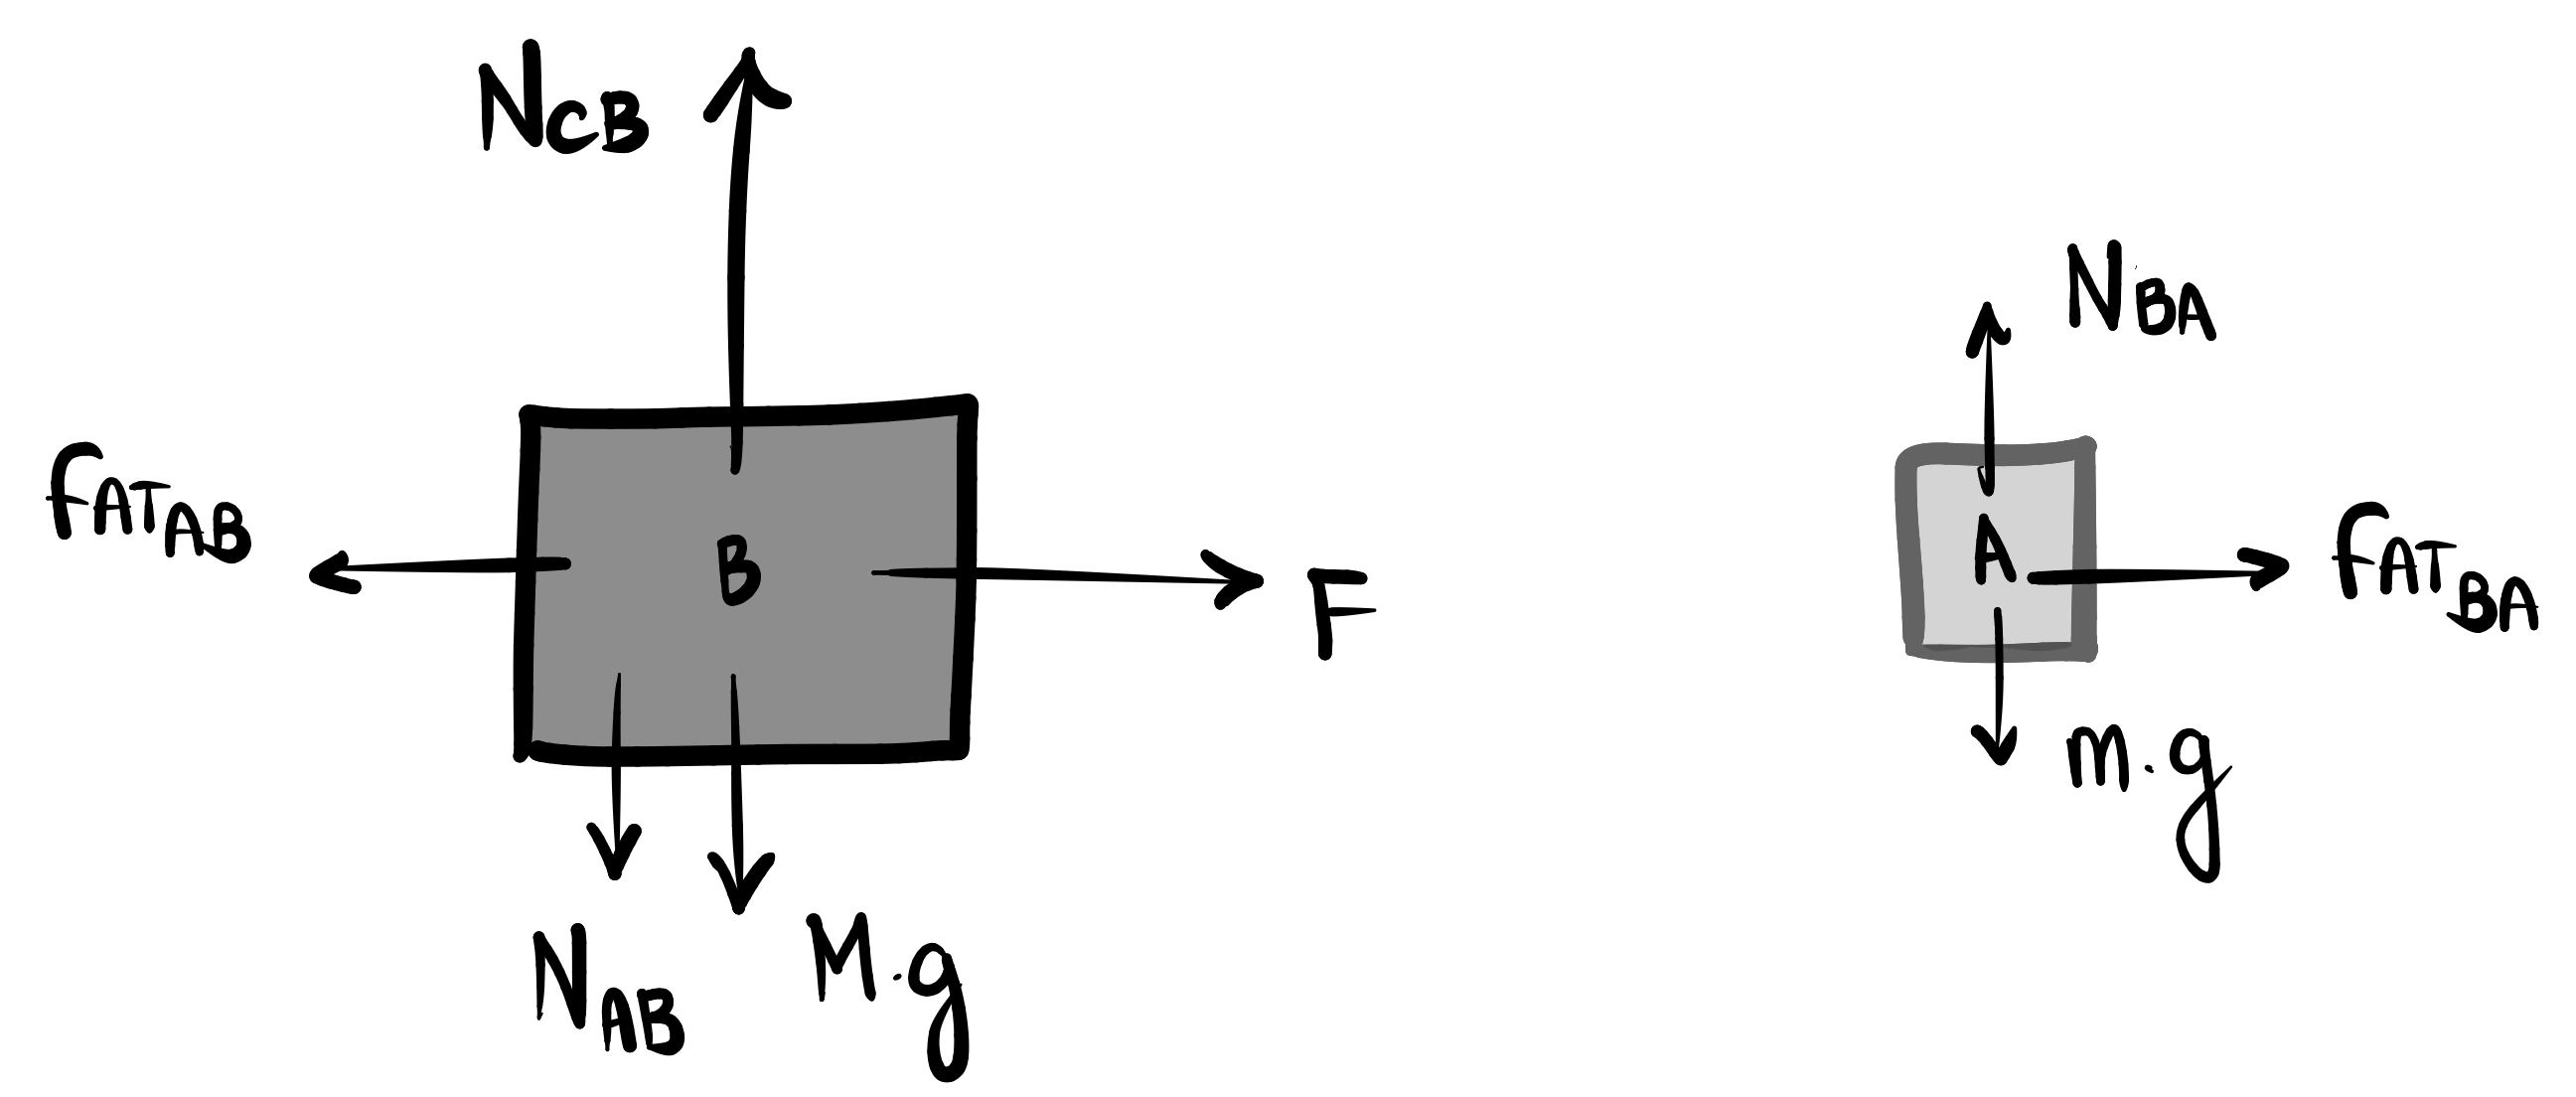
\includegraphics[width=0.6\linewidth]{imagensdinamicanewton/atritoestaticomovendo2.png}};
  \end{scope}
\end{tikzpicture}
\captionof{figure}{Análise das forças que atuam nos blocos que se movem com a mesma aceleração horizontal $a.$}
\label{fig_mec_atritoestaticomovendo2}
} 
\vspace{0.3cm}

Como o bloquinho não se move na vertical, há equilíbrio nessa direção:

$$ F_{Ry} = 0 \implies N_{BA} = mg.$$

Já na horizontal a resultante das forças tem que ser capaz de gerar no bloquinho a mesma aceleração $a$ para a direita que o bloco maior possui, para que eles estejam em repouso relativo:

$$ F_{Rx} = ma \implies F_{AT_{AB}} = ma.$$

Usando as duas equações acima na desigualdade $F_{AT} \leq \mu_e N$ temos

$$ ma \leq \mu_e mg \implies \boxed{a \leq \mu_e g, }$$

\noindent ou seja, o maior valor possível de aceleração para que tal situação seja possível é $a_\text{max}= \mu_e g.$

Para acelerações superiores a essa o atrito estático não conseguirá segurar o bloquinho em repouso em relação ao bloco maior e ele começará a escorregar para a esquerda em relação a tal bloco. Note como tal relação faz sentido: 

\begin{enumerate}
    \item [(i)] a aceleração máxima é proporcional a $\mu_e$. Isso quer dizer que, quanto maior o coeficiente de atrito, maior pode ser a aceleração máxima que o sistema pode ter de modo que os blocos não escorreguem um em relação ao outro. Isso faz total sentido, haja vista que é o próprio atrito quem está impedindo que haja movimento relativo entre os blocos, e $\mu_e$ é justamente o número que mede o quão acoplados os blocos estão.

    \item [(ii)] além disso, a aceleração máxima também é proporcional à gravidade. Isso ocorre porque, quanto mais intensa for a gravidade, maior será o ``\textit{acoplamento}'' entre os dois blocos, uma vez que maior será a força (peso) que puxa um bloco contra o outro (ou seja, a normal será maior). Em um local de menor gravidade os blocos estão menos ``\textit{grudados}'' um com o outro e, portanto, a aceleração máxima que o sistema pode ter para que os blocos permaneçam em repouso relativo é menor.
\end{enumerate}







Por fim, representamos também na Figura \ref{fig_mec_atritoestaticomovendo2}, a título de deixar completa a análise, as forças no bloco $B.$ Elas são desnecessárias para a análise deste problema, mas, para o leitor mais curioso, são elas: $N_{CB}$ é a normal trocada entre o bloco $B$ e o chão. Sua reação tem o mesmo módulo e atua no chão. $F$ seria a força feita pelo menino no bloco, $Mg$ é o peso do bloco e as demais forças já foram discutidas.

\vspace{0.3cm}

\begin{exemplo}[Nível I]\label{exemplo_newton_fatestatico01}

Um bloco de massa $m$ é comprimido contra uma parede vertical, como mostra a Figura \ref{fig_mec_fatestaticoex011} por uma força $F.$ O atrito entre a parede vertical e o bloco é tal que o coeficiente de atrito vale $\mu.$ 

\vspace{0.3cm}
{
\centering
\begin{tikzpicture}
  \begin{scope}[blend mode=multiply]
    \node {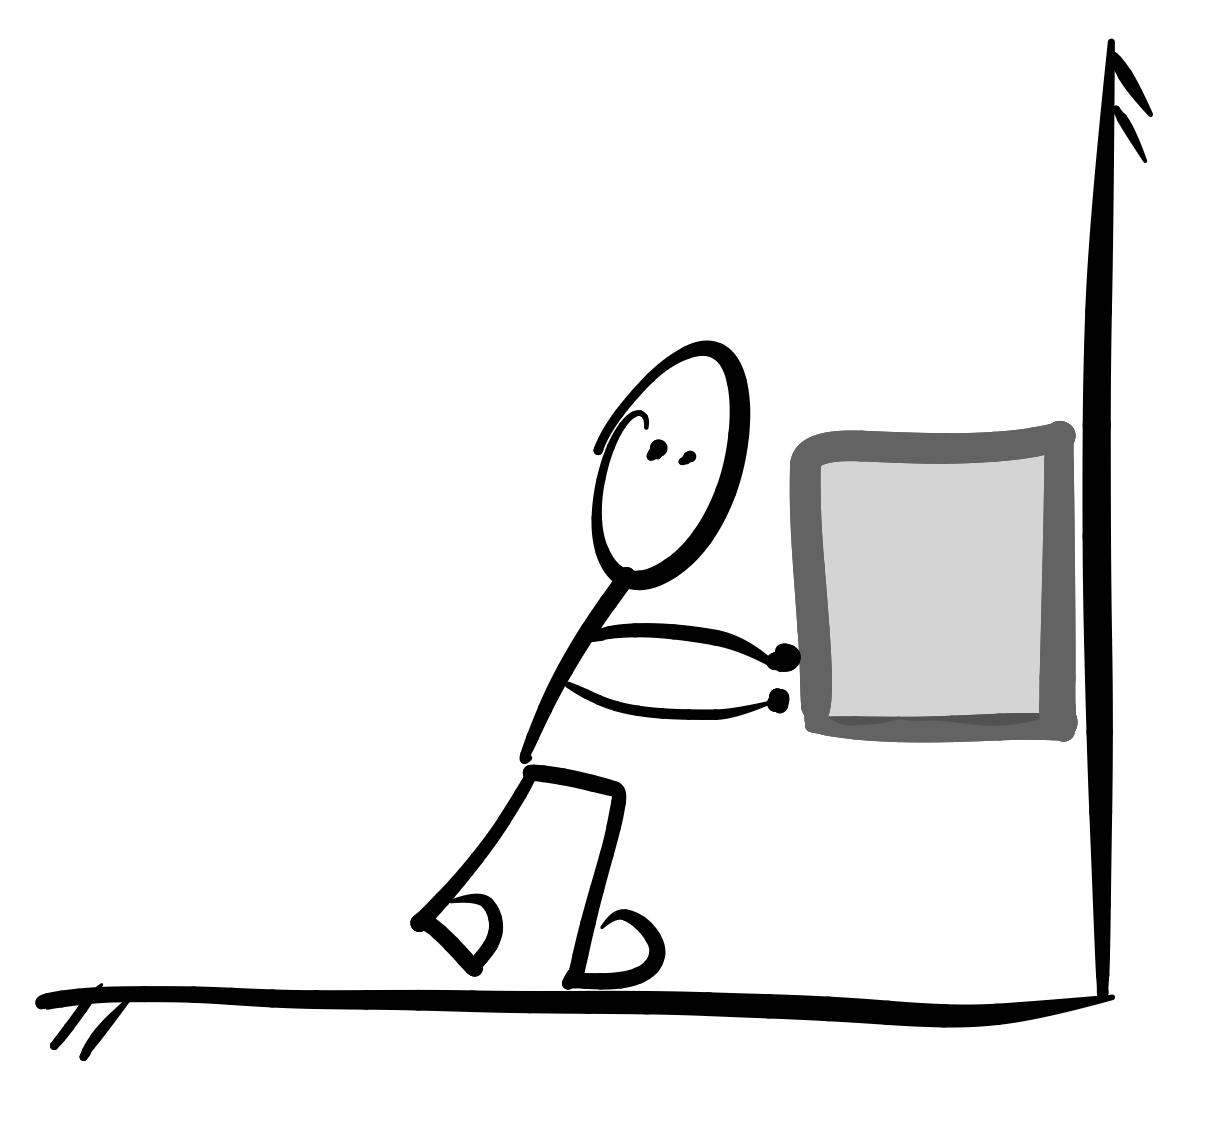
\includegraphics[width=0.25\linewidth]{imagensdinamicanewton/fatestaticoex011.png}};
  \end{scope}
\end{tikzpicture}
\captionof{figure}{}
\label{fig_mec_fatestaticoex011}
} 
\vspace{0.3cm}



Se a gravidade local vale $g$, calcule a menor força $F$ que deve ser feita no bloco para que ele fique em equilíbrio quando

\begin{itemize}
    \item [a)] $m=2$ kg e $\mu_e = 0.5.$
    \item [b)] $m=10$ kg e $\mu_e=0.5.$
    \item [c)] $m=10$ kg e $\mu_e=0.8.$
    \item [d)] $m$ e $\mu$ quaisquer.
\end{itemize}


\resolucao

Como queremos o bloco em equilíbrio, para as situações dos quatro itens trabalharemos no regime de atrito estático, e o diagrama de forças no bloco será aquele da Figura \ref{fig_mec_fatestaticoex012}. 

O menino faz uma força $F,$ horizontal para a direita, comprimindo o bloco contra a parede. Com isso, o bloco empurra a parede para a direita com uma força normal $N$, e, pela Terceira Lei de Newton, a parede faz uma força $N$ para a esquerda no bloco. A figura também representa seu peso $P=mg,$ que atua verticalmente para baixo. Como a tendência do bloco é escorregar parede abaixo, o atrito, contrariando tal tendência, atua para cima.

\vspace{0.3cm}
{
\centering
\begin{tikzpicture}
  \begin{scope}[blend mode=multiply]
    \node {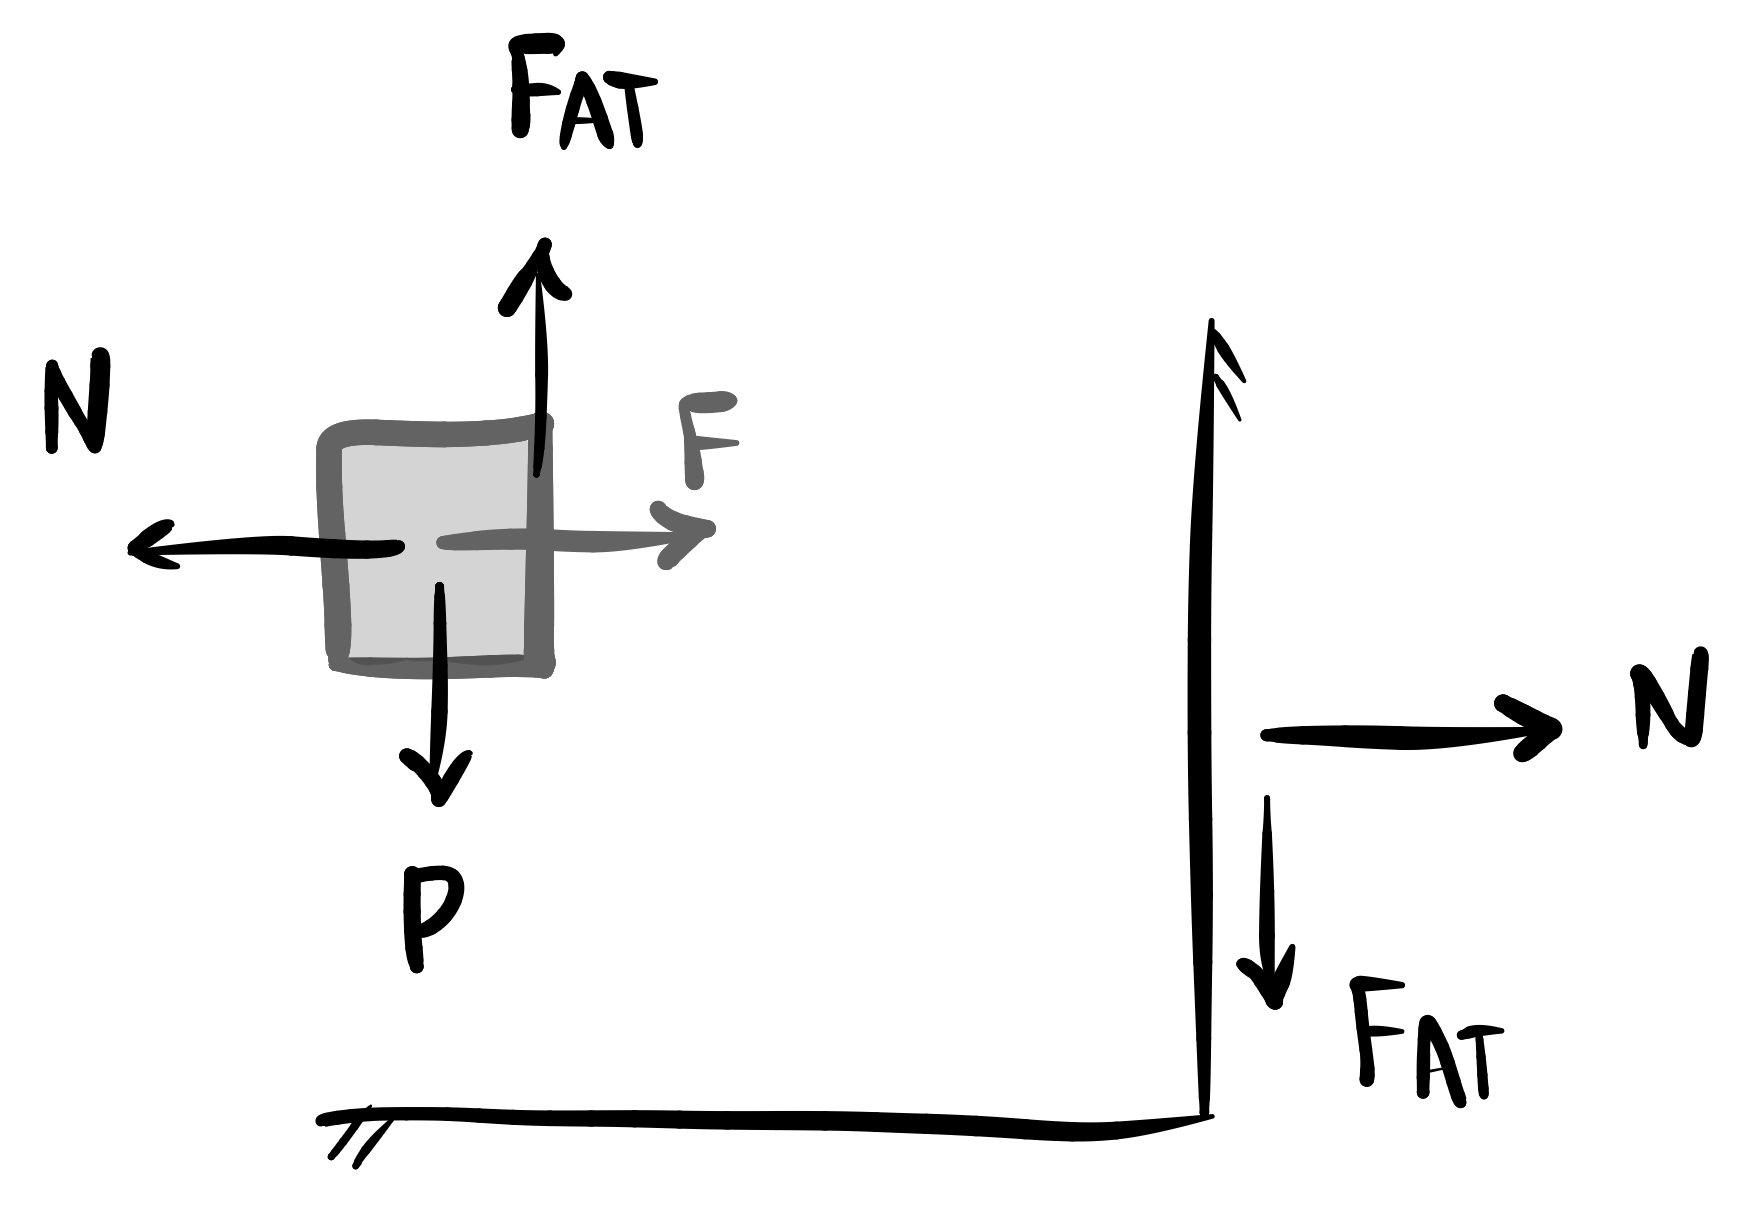
\includegraphics[width=0.3\linewidth]{imagensdinamicanewton/fatestaticoex012.png}};
  \end{scope}
\end{tikzpicture}
\captionof{figure}{Diagrama de forças no bloco e reações na parede.}
\label{fig_mec_fatestaticoex012}
} 
\vspace{0.3cm}

Vamos analisar agora cada situação:


\begin{itemize}
    \item [a)] $m=2$ kg e $\mu = 0.5.$

    Neste caso o peso é $P=mg = 20$N. Na horizontal as forças vão se anular, haja vista o equilíbrio do bloco. Logo, teremos que $N=F.$

    Sabemos que $F_{\text{AT}} \leq \mu_e N$, logo:


    $$ F_{\text{AT}} \leq \mu_e F \implies F \geq \dfrac{F_{\text{AT}}}{\mu_e},  $$


   \noindent contudo, sabemos também que precisamos ter -- do equilíbrio vertical do bloco -- $F_\text{AT}=P=20$N, logo

   $$  F \geq \dfrac{F_{\text{AT}}}{\mu_e} \implies F \geq \dfrac{20}{0.5} \implies \boxed{F \geq 40 \text{ N.}} $$

   Ou seja, a menor força $F$ com que se deve empurrar o bloco contra a parede para que ele não escorregue e fique em equilíbrio é de 40N.
    
    \item [b)] $m=10$ kg e $\mu=0.5.$


    O raciocínio aqui é idêntico ao anterior, só mudando o valor do peso $P$ do bloco, que trocaremos de 20N para 100N:

    $$  F \geq \dfrac{F_{\text{AT}}}{\mu_e} \implies F \geq \dfrac{100}{0.5} \implies \boxed{F \geq 200 \text{ N.}} $$

    Ou seja, a menor força $F$ com que se deve empurrar o bloco contra a parede para que ele não escorregue e fique em equiíbrio é de 200N. Como temos o mesmo coeficiente de atrito e um bloco mais pesado, é natural esperar que tenhamos que comprimi-lo com mais intensidade contra a parede para mantê-lo em equilíbrio. \footnote{Perceba a física do problema: já intui-se que, para manter um bloco mais pesado em repouso dessa forma será necessário comprimi-lo com ainda mais intensidade contra a parede vertical. De fato isso ocorre, porque quanto maior é a intensidade com que se empurra o bloco contra a parede (força $F),$ maior é a compressão do bloco contra a parede (força normal $N$ e, como sabemos, o atrito entre duas superfícies é proporcional ao quanto elas estão comprimidas uma contra a outra -- força normal). Assim, quanto mais intenso for a força $F$ que comprime o bloco na parede, maior será o atrito capaz de segurar o bloco de escorregar para baixo.}
    
    \item [c)] $m=10$ kg e $\mu=0.8.$

     O raciocínio aqui é idêntico ao anterior, só mudando o valor do coeficiente de atrito, que foi usado apenas no último passo do cálculo:

    $$  F \geq \dfrac{F_{\text{AT}}}{\mu_e} \implies F \geq \dfrac{100}{0.8} \implies \boxed{F \geq 125 \text{ N.}} $$

    
      Ou seja, a menor força $F$ com que se deve empurrar o bloco contra a parede para que ele não escorregue e fique em equiíbrio é de 125N. Como o coeficiente de atrito é maior, a normal também pode ser menor para que se gere o mesmo atrito capaz de sustentar o peso do bloco.
    
    \item [d)] $m$ e $\mu$ quaisquer.

      Usando que $F_{\text{AT}} = P=mg$ e a desigualdade $ F \geq \dfrac{F_{\text{AT}}}{\mu_e} $, chegamos em

      $$ F \geq \dfrac{mg}{\mu_e}. $$


       Ou seja, quanto maior o valor de massa $m$ maior é a força $F$ horizontal necessária para gerar atrito suficiente de modo que o bloco fique em repouso, como esperávamos. Além disso, quanto maior o coeficiente de atrito estático $\mu_e,$ menor é o valor de tal força, como também era esperado.
    
\end{itemize}





\end{exemplo}


\vspace{0.3cm}


\begin{exemplo}[Nível II]\label{exemplo_newton_fatestatico02}

Considere um trem e um bloco de massa $m$, colocado na sua dianteira. Se a gravidade é vertical e seu módulo vale $g$ e o coeficiente de atrito estático entre o bloco e o vagão vale $\mu,$ qual é a menor aceleração $a$ que o trem deve ter para que ele consiga se mover sem que o bloco escorregue em relação a ele?

\vspace{0.3cm}
{
\centering
\begin{tikzpicture}
  \begin{scope}[blend mode=multiply]
    \node {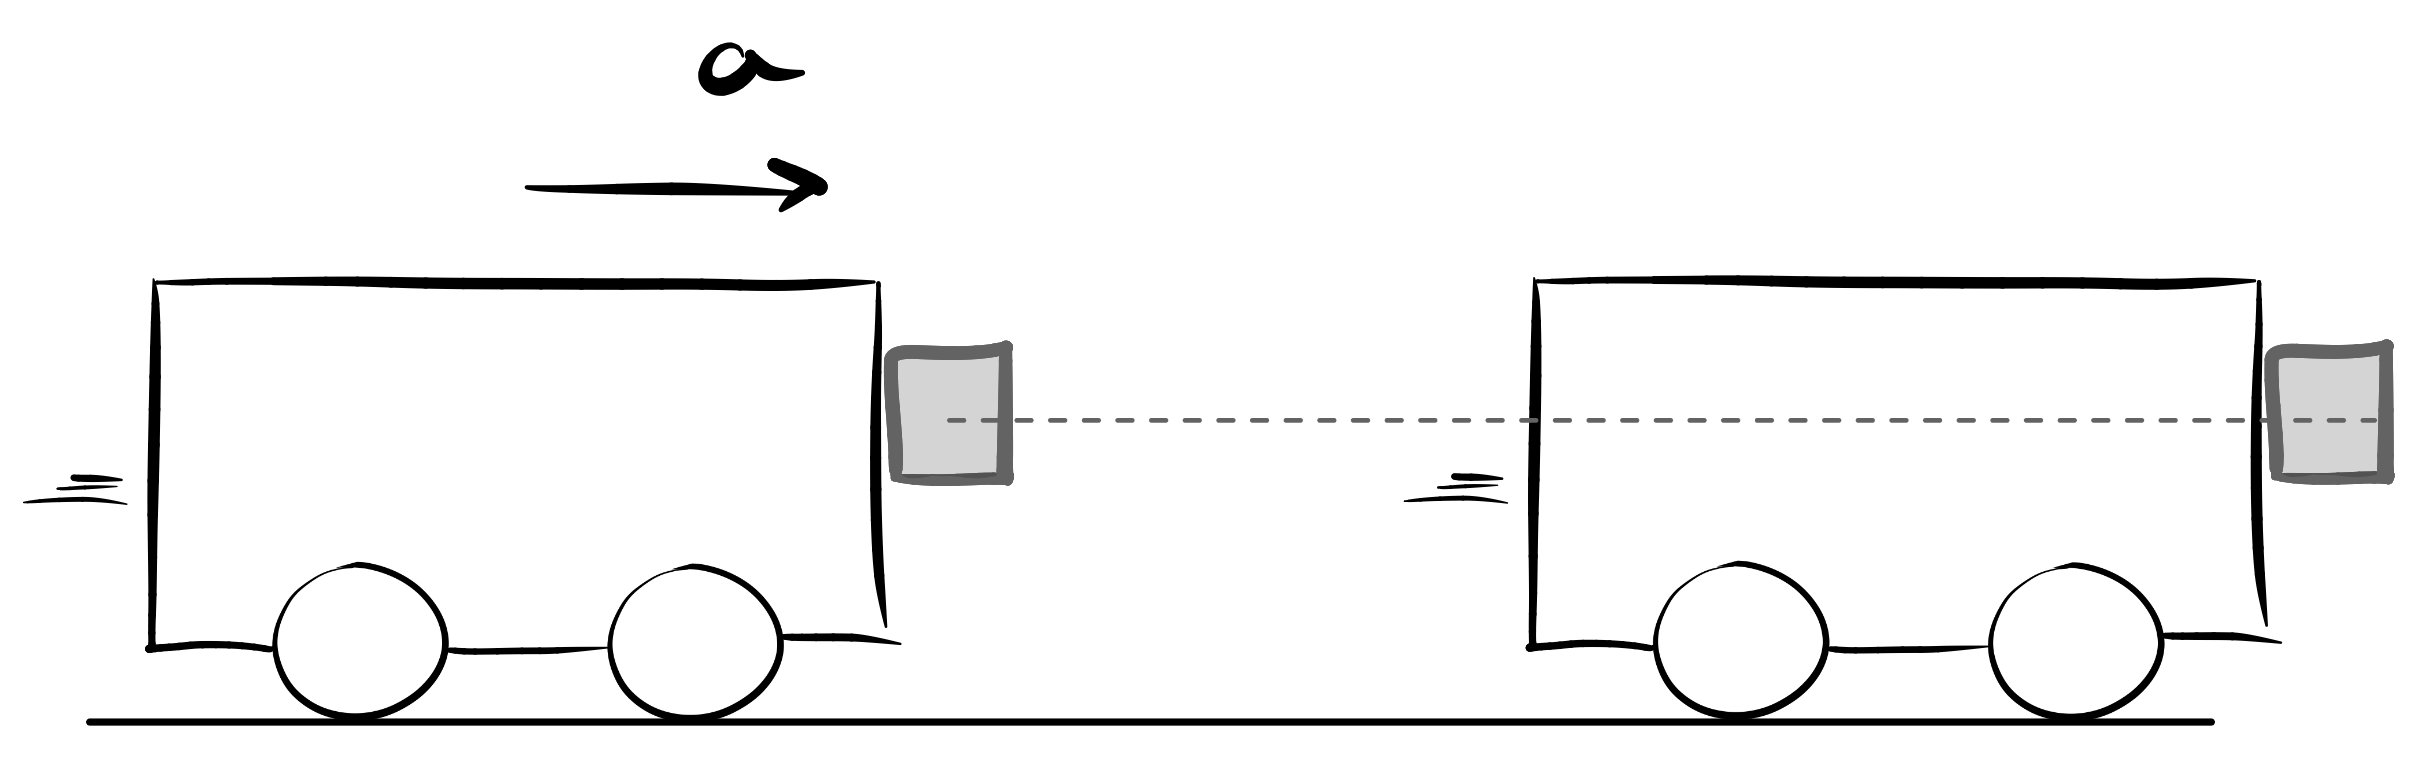
\includegraphics[width=0.6\linewidth]{imagensdinamicanewton/fatvagaoetrem1.png}};
  \end{scope}
\end{tikzpicture}
\captionof{figure}{}
\label{fig_mec_fatvagaoetrem1}
} 


\resolucao

Avaliemos as forças no bloco de massa $m$. Temos o seu peso, atuando verticalmente para baixo. A normal $N$ de compressão entre o bloco e a parede vertical do vagão, sempre perpendicular à superfície de contato. E, temos também a força de atrito $F_{\text{AT}}$, que atua para cima, uma vez que a tendência do bloco é escorregar para baixo (por conta da gravidade).

\vspace{0.3cm}
{
\centering
\begin{tikzpicture}
  \begin{scope}[blend mode=multiply]
    \node {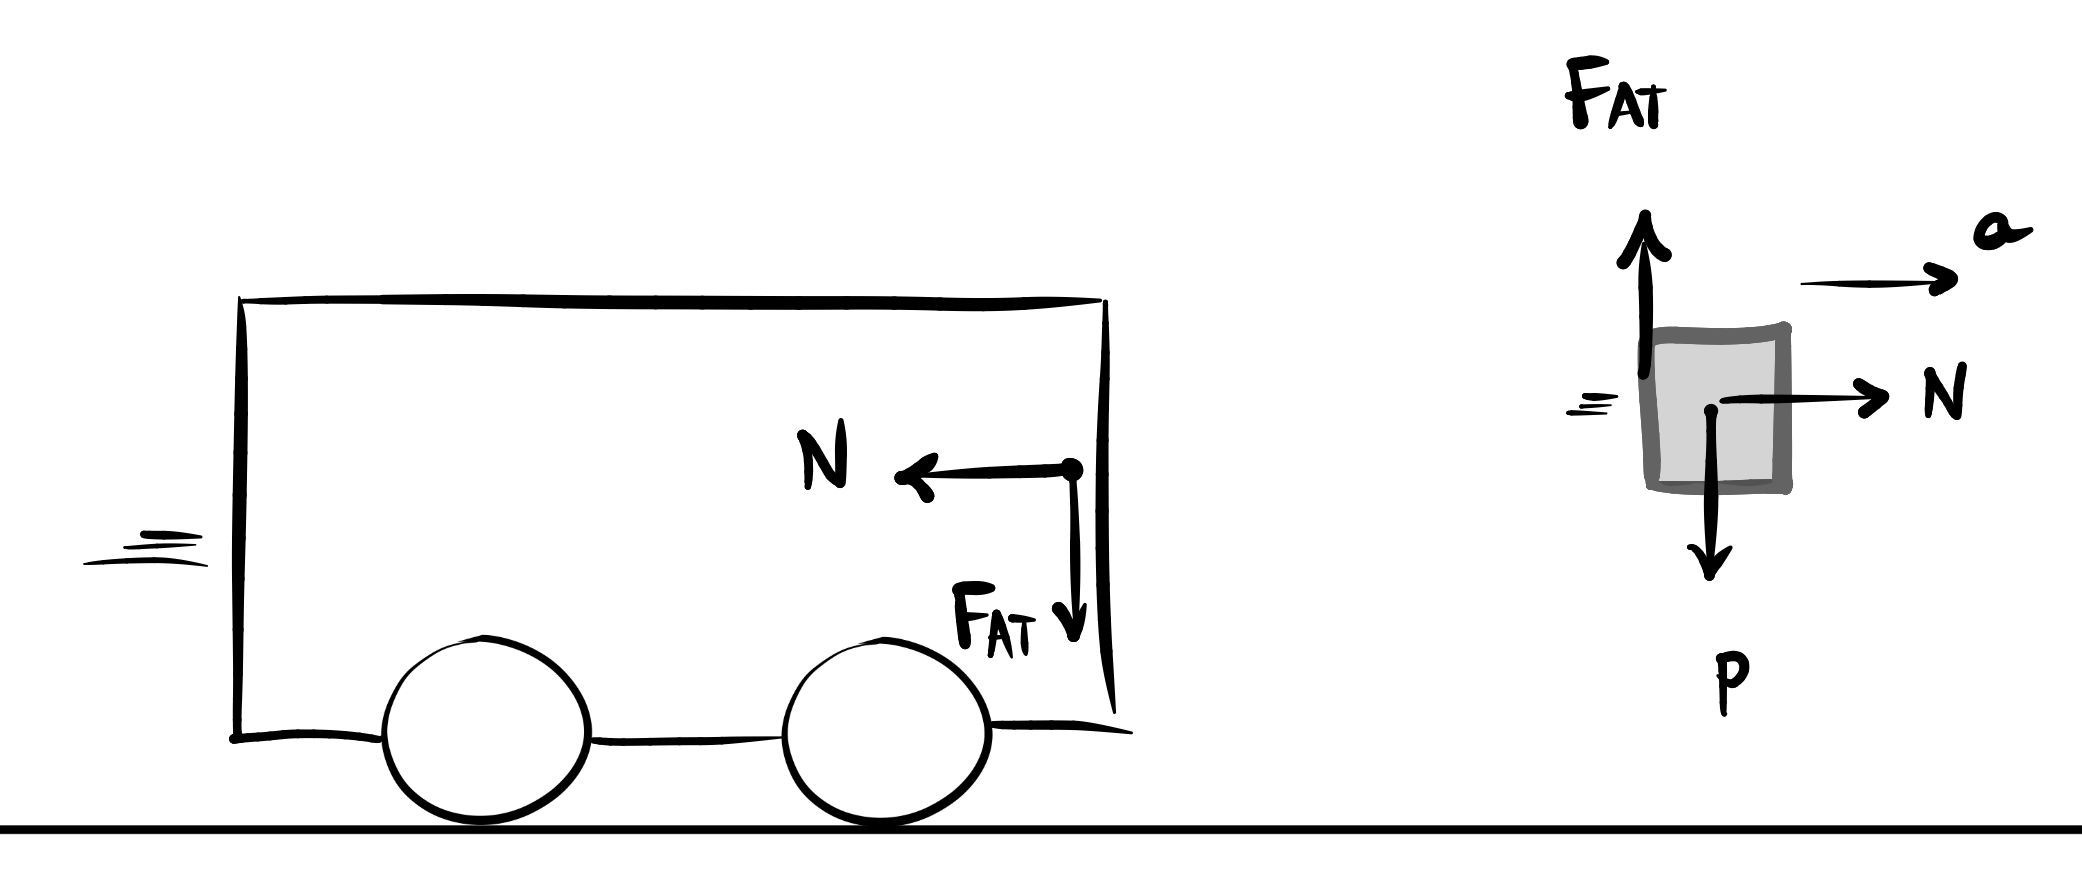
\includegraphics[width=0.6\linewidth]{imagensdinamicanewton/fatvagaoetrem2.png}};
  \end{scope}
\end{tikzpicture}
\captionof{figure}{Diagrama de forças da situação.}
\label{fig_mec_fatvagaoetrem2}
} 
\vspace{0.3cm}

Se o bloco não se move em relação ao vagão isso significa que

\begin{enumerate}
    \item [(i)] O bloco não se move na vertical, uma vez que o vagão não possui movimento vertical. Logo, as forças no bloco se equilibram na vertical: $F_{\text{AT}}=P=mg.$

    \item [(ii)] O bloco compartilha exatamente do mesmo movimento que o vagão na horizontal, isto é, ele se move horizontalmente com a mesma aceleração $a$ do vagão:

    $$ F_{\text{Rx}} = ma \implies N = ma.$$

    Assim, garantimos que o bloco não se move em relação ao vagão.
\end{enumerate}

Inserindo os dois resultados acima na desigualdade $F_{\text{AT}} \leq \mu_e N$ somos levados a

 $$ mg \leq \mu_e ma \implies \boxed{a \geq \dfrac{g}{\mu_e} .}$$

 Ou seja, a menor aceleração a ser imprimida no vagão de modo que a caixa fique \textit{grudada} nele e não escorregue é exatamente igual a $a = \sfrac{g}{\mu_e.}$ \footnote{Note que não é simples executar tal façanha, uma vez que para a quase totalidade dos casos teremos $0 < \mu_e < 1$. Logo, a aceleração horizontal que o vagão precisaria ter seria, em geral, maior do que a da gravidade. No caso em que $\mu_e = 0.5,$ por exemplo, seria necessário imprimir no vagão uma aceleração horizontal igual a $\sfrac{g}{0.5} = 2g$, ou seja, o dobro da aceleração da gravidade, o que é uma aceleração bastante alta. A título de comparação, a aceleração máxima de um carro comum gira em torno de 2 m/s$^2$ e 4 m/s$^2$.}

\end{exemplo}


\vspace{0.3cm}

\begin{exemplo}[Nível III]\label{exemplo_newton_fatestatico03}

A caixa de massa $M$ está apoiada sobre o solo, como mostra a Figura \ref{fig_mec_fatestaticoex03}. Sendo $\mu$ o coeficiente de atrito estático entre tais superfícies e $g$ a aceleração da gravidade, mostre que a menor força $F$ capaz de mover a caixa é aquela para o qual $\phi = \arctan (\mu).$


\vspace{0.3cm}
{
\centering
\begin{tikzpicture}
  \begin{scope}[blend mode=multiply]
    \node {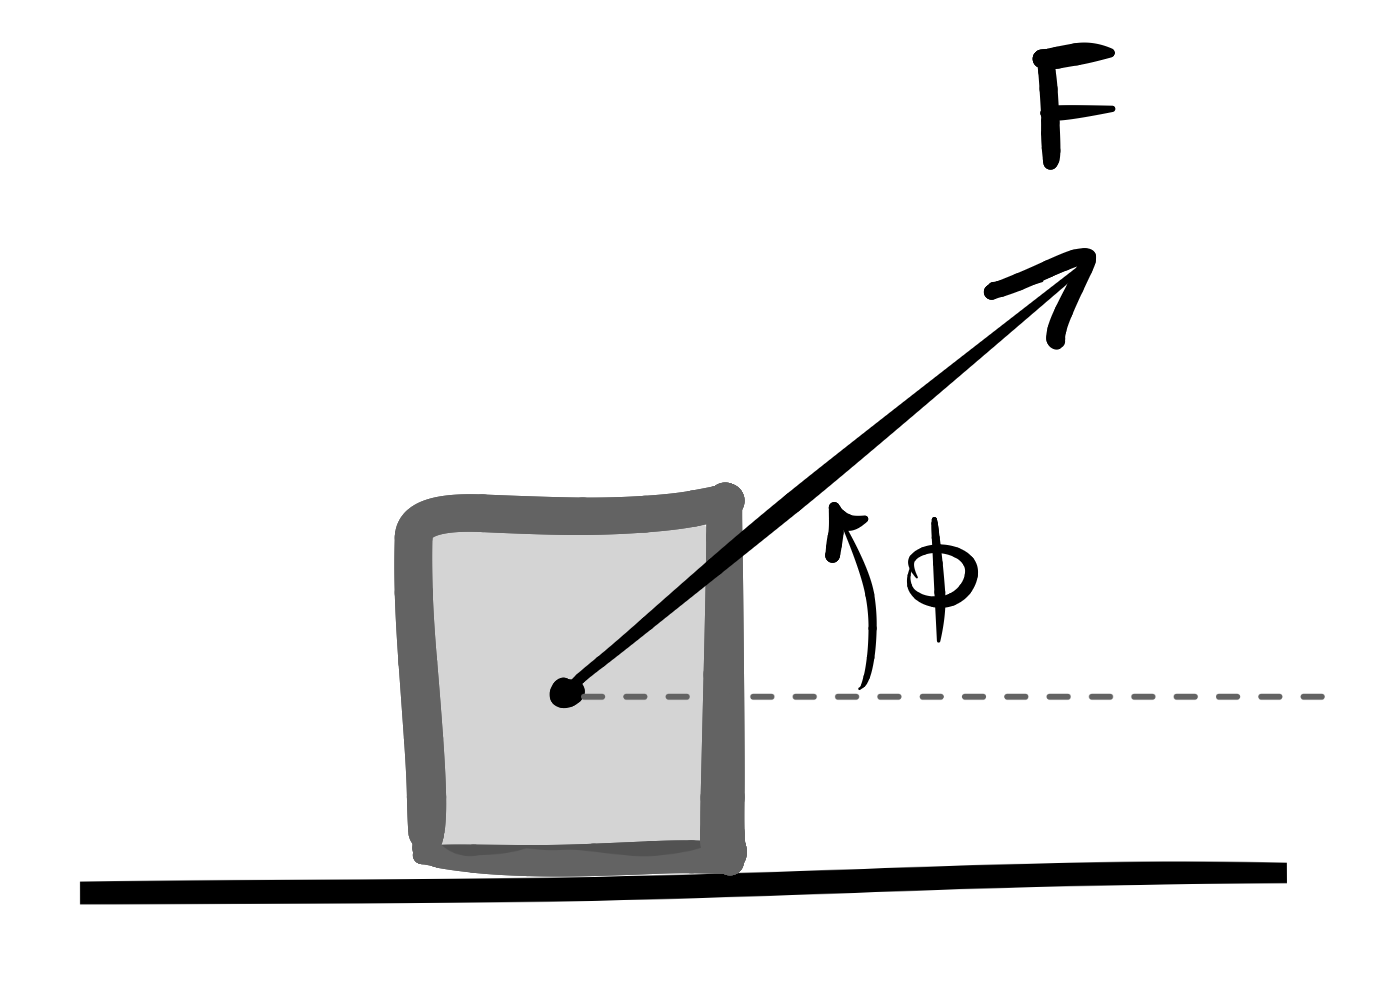
\includegraphics[width=0.3\linewidth]{imagensdinamicanewton/fatestaticoex03.png}};
  \end{scope}
\end{tikzpicture}
\captionof{figure}{}
\label{fig_mec_fatestaticoex03}
} 
\vspace{0.3cm}


\resolucao


O equilíbrio de forças exige que 

$$ F_\text{R} = 0 \begin{cases}
    F_{\text{R}_x} = 0 \implies  F \cos \phi = F_\text{AT} \\
    F_{\text{R}_y} = 0 \implies  F \sin \phi + N = Mg \implies N= Mg - F \sin \phi 
\end{cases}$$

Se a caixa está quase se movendo, então estamos na condição de \emph{iminência de movimento,} e o atrito é o estático máximo:

$$ F_\text{AT} = \mu N \implies F \cos \phi =  \mu Mg - \mu F \sin \phi, $$

\noindent ou seja:

$$ F (\cos \phi + \mu \sin \phi) = \mu Mg \implies F = \dfrac{\mu Mg}{(\cos \phi + \mu \sin \phi).}$$

Procuramos encontrar a \emph{menor} força $F$ possível. Ora, note que $\mu$, $M$ e $g$ -- os termos que compõem o numerador da expressão acima -- são constantes. Logo, $F$ assume valores diferentes por conta dos diferentes ângulos $\phi$ com os quais ela pode ser feita, ou seja, temos uma força $F(\phi).$ Desse modo, quanto \emph{maior} for o denominador, menor será o valor de tal força. Assim, nosso problema se reduz a \emph{maximizar} o valor da expressão

$$ f(\phi) = \cos \phi + \mu \sin \phi.$$

Tal expressão pode ser reescrita como

$$ f(\phi) = \sqrt {\mu^2 +1} \left( \dfrac{1}{\sqrt {\mu^2 +1}}\cos \phi + \sin \phi \dfrac{\mu}{\sqrt {\mu^2 +1}} \right).$$

Note, contudo, pelo triângulo abaixo, que
$$ \sin \alpha = \dfrac{1}{\sqrt {\mu^2 +1}} \quad \text{ e } \quad \cos \alpha = \dfrac{\mu}{\sqrt {\mu^2 +1}}, $$

\noindent em que $\alpha$ é um ângulo fixo, dependente do fator $\mu$, dado por $\alpha = \arctan (\mu^{-1})$. Assim, a expressão de $f(\phi)$ pode ser reescrita como

$$ f(\phi) = \sqrt {\mu^2 +1}  \left( \sin \alpha \cos \phi + \sin \phi \cos \alpha    \right) \implies f(\phi) = \sqrt {\mu^2 +1} \sin (\phi + \alpha).$$

\vspace{0.3cm}

\begin{center}
    

\begin{tikzpicture}[scale=2]
    % Pontos (catetos com comprimentos próximos)
    \coordinate (A) at (0,0);
    \coordinate (B) at (1.2,0);
    \coordinate (C) at (1.2,1);

    % Triângulo
    \draw[thick] (A) -- (B) -- (C) -- cycle;

    % Ângulo reto em B
    \draw[thick] (1.05,0) -- (1.05,0.15) -- (1.2,0.15);

    % Ângulo alpha em A
    \draw[thick] (0.35,0) arc[start angle=0,end angle=40,radius=0.35];

    % Rótulos dos lados
    \node[below] at (0.6,0) {$\mu$};
    \node[right] at (1.2,0.5) {$1$};
    \node[above left] at (0.6,0.5) {$\sqrt{\mu^2+1}$};

    % Rótulo do ângulo alpha
    \node at (0.5,0.18) {$\alpha$};
\end{tikzpicture}


\end{center}






Ora, como dito, o ângulo $\alpha$ é um ângulo fixo, determinado de forma única pelo parâmetro $\mu.$ De toda forma, ainda que não o fosse, o fato é que $\sin (\phi+\alpha),$ quaisquer que sejam os valores de $\phi$ e $\alpha,$ é sempre uma expressão cujo máximo valor é 1:

$$ -1 \leq \sin (\phi+\alpha) \leq 1.$$

Desse modo, multiplicando a desigualdade por $\sqrt {\mu^2 +1}$, teremos:

$$ - \sqrt {\mu^2 +1} \leq f(\phi) \leq \sqrt {\mu^2 +1},$$

\noindent de onde vemos que o valor \emph{máximo} de $f(\phi)$ é $\sqrt {\mu^2 +1}$, o que ocorre quando o seno é um:

$$ \sin (\phi + \alpha) = 1 \implies \phi + \alpha = \dfrac{\pi}{2} \implies \phi = \dfrac{\pi}{2} - \alpha.$$

Logo, tem-se

$$ \tan (\phi) = \tan \left(\dfrac{\pi}{2} - \alpha \right) = \dfrac{1}{\tan (\alpha)} = \mu, $$

\noindent ou seja, $\phi = \arctan (\mu),$ como queríamos demonstrar.

Munidos do ângulo que fornece a força mínima, de $\tan \phi = \mu$ extraímos que $\sin \phi = \mu/\sqrt{1+\mu^2}$ e $\cos \phi = 1/\sqrt{1+\mu^2}$, de modo que a força mínima é


$$F (\phi)= \dfrac{\mu Mg}{(\cos \phi + \mu \sin \phi)} \implies \boxed{F_\text{MIN} = \dfrac{ Mg \mu\sqrt{1+\mu^2}}{1+\mu^2}.}$$


\end{exemplo}








\begin{secnivel}[Força de Atrito Cinético]{I}{Força de Atrito Cinético}
  
  \eqLdois{exp}{eq_newton_fatcinetico}{F_{\text{AT}_\text{C} }= \mu_{c} N}

\end{secnivel}






\secgfe{De onde vem}

Considere a situação da Figura \ref{fig_mec_fatestaticovariavel}. Constatamos que a força de $80$N era o maior valor de força que o atrito estático poderia fazer, mantendo, assim, o bloco em situação de equilíbrio estático. O que aconteceria se continuássemos a imprimir no bloco uma força $F$ maior que $80$N? Ora, naturalmente, ele entraria em movimento, e o atrito estático deixaria de existir.



O atrito, contudo, que possui origem nas imperfeições, rugosidades e saliências da estrutura da matéria, continuaria existindo, só mudaria de regime: a força de atrito que atua quando há movimento relativo entre as superfícies é o atrito cinético. O seu módulo, direção, sentido e sua origem são exatamente os mesmos daqueles discutido no desenvolvimento da Equação \eqref{eq_newton_fatestatico}.

Note que a estrutura da Equação \eqref{eq_newton_fatcinetico} é exatamente a mesma da Equação \eqref{eq_newton_fatestatico}, de modo que é natural compreendê-la à luz da discussão feita sobre o atrito estático. O que muda aqui são, essencialmente, duas coisas:

\begin{enumerate}
    \item [(i)] O coeficiente de atrito cinético, $\mu_c$, é, em geral, diferente do coeficiente de atrito estático. Experimentos mostram que 

    $$ \mu_e \geq \mu_c,$$

    \noindent ou seja, a força de atrito estático máxima é maior do que a força de atrito cinético. Isso é razoável de se compreender, uma vez que, no repouso, há maior intertravamento microscópico entre as superfícies. Já ao iniciar o movimento, essas ``\textit{ligações}'' são rompidas, fazendo com que o efeito do atrito seja menor.

    \item [(ii)] A força de atrito cinético é constante, e seu módulo é dado pela Equação \eqref{eq_newton_fatcinetico}. Diferente do atrito estático, que tem módulo variável e admite um valor máximo, o atrito cinético possui módulo constante. 
    
    Isso está indicado no gráfico da Figura \ref{fig_mec_fatcineticografico}: ao fazer sob o bloco uma força maior do que o atrito estático consegue igualar para mantê-lo em equilíbrio, o bloco começa a se mover. Tão logo isso ocorre, o atrito entra em regime cinético, de modo que seu valor cai (porque $\mu_e \geq \mu_c)$ e fica constante. No caso, para $40$N, mas tal valor é ilustrativo -- não há necessidade alguma da força de atrito cinético ser exatamente metade da força de atrito estático máxima.
\end{enumerate}



{
\centering
\begin{tikzpicture}
  \begin{scope}[blend mode=multiply]
    \node {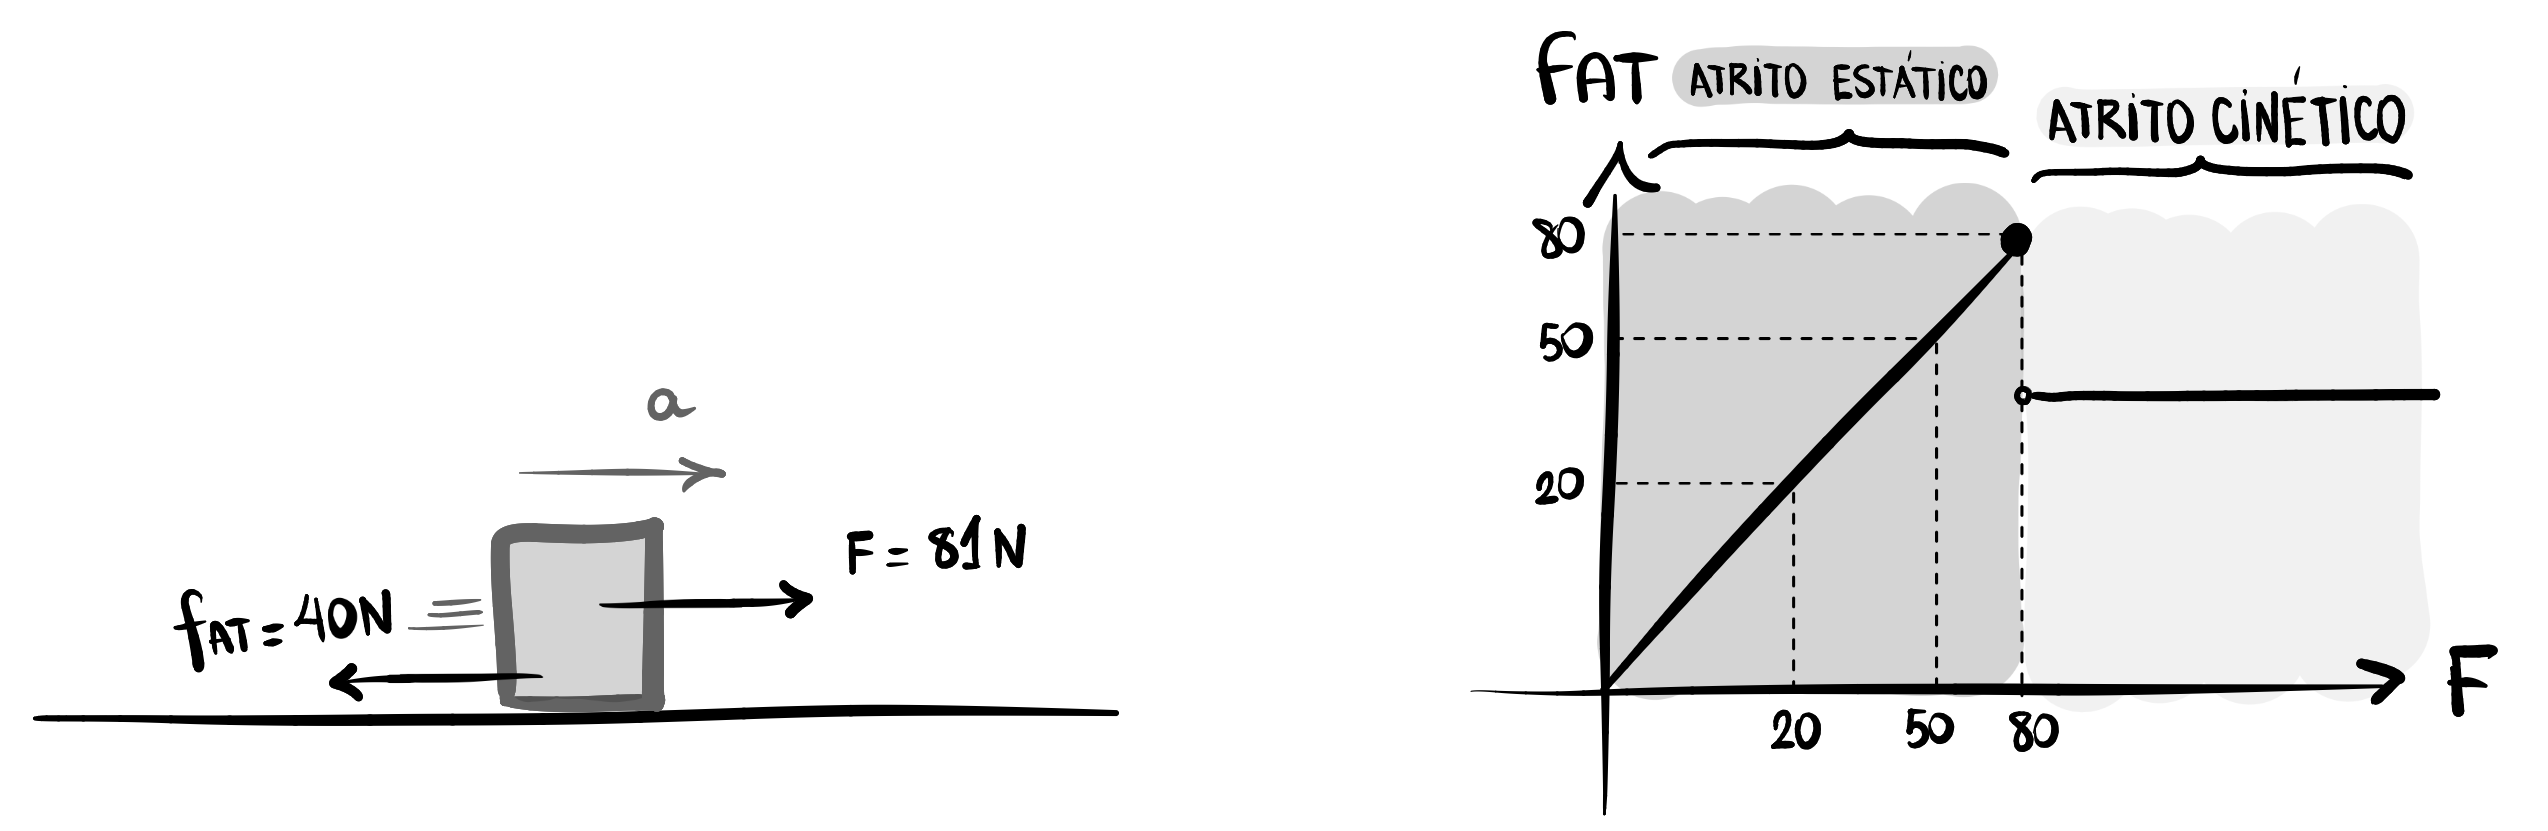
\includegraphics[width=0.8\linewidth]{imagensdinamicanewton/fatcineticografico.png}};
  \end{scope}
\end{tikzpicture}
\captionof{figure}{O regime de atrito cinético e estático.}
\label{fig_mec_fatcineticografico}
} 
\vspace{0.3cm}




\secgfe{Onde é usada}

Basicamente em todo contexto em que dois corpos em contato possuem suas superfícies de contato em movimento relativo. 

Uma aplicação extremamente elegante da Física no cotidiano é o sistema de freios ABS (\textit{Anti-lock Braking System}). Para compreendê-lo corretamente, precisamos antes esclarecer uma ideia que costuma confundir muitos estudantes: \textit{por que o atrito entre o pneu e o solo é estático, se o carro está em movimento?}

Pois é. O leitor desatento poderia imaginar que, uma vez que o carro se move em relação ao chão, o atrito entre o solo e os pneus do carro seria o cinético. Mas, em geral, é o estático -- desde que não haja deslizamento (derrapagem).


Quando um carro se desloca com as rodas rolando sem deslizar, cada ponto do pneu descreve um movimento circular em torno do eixo da roda. No entanto, o ponto específico do pneu que está em contato com o solo possui, naquele instante, velocidade nula em relação ao chão. É como se o ponto do pneu em contato com o chão estivesse momentaneamente em repouso e toda a roda girasse em torno daquele ponto. \\



Logo, se o ponto do pneu em contato com o chão está em repouso instantâneo -- ou seja, é um rolamento sem deslizamento --, não há movimento relativo entre o pneu e o solo e, portanto, o atrito que atua é o estático.

Mas o que acontece quando a roda trava? Se o motorista freia bruscamente e a roda trava, ela para de girar. O carro continua avançando por inércia, mas agora o ponto de contato do pneu passa a deslizar sobre o asfalto: o carro começa a derrapar.

Nesse momento há movimento relativo entre as superfícies, de modo que o atrito deixa de ser estático e passa a atuar o \textbf{atrito cinético}. E aqui surge um ponto crucial da Física que já levantamos
\[
\mu_e > \mu_c,
\]

\noindent ou seja, o coeficiente de atrito estático é maior que o cinético. Isso significa que, quando a roda trava, a força de atrito disponível diminui -- entra no regime cinético. A frenagem fica menos eficiente, a distância de frenagem aumenta e o motorista perde controle direcional. 

Este seria o funcionamento de um carro sem freios ABS, e está ilustrado no primeiro gráfico da Figura \ref{fig_mec_fatcABS}, já conhecido por nós, em que a força $F$ aqui representaria a força com que o motorista pressiona os freios, que é o que vai gerar a compressão do disco de freio contra a roda do carro.

No carro sem freio ABS, inicialmente, a força de atrito ($F_{\text{AT}}$) cresce proporcionalmente à força aplicada ($F$). Ela se ajusta exatamente ao valor necessário para impedir o deslizamento. No gráfico, isso corresponde à reta crescente até o valor máximo (por exemplo, $80\,\text{N}$). Esse ponto representa o \textbf{atrito estático máximo}.

Se a força aplicada ultrapassa esse limite, ocorre o escorregamento. A força de atrito sofre uma queda abrupta para um valor menor. No gráfico, essa queda aparece como a passagem do ponto superior (por exemplo, $80\,\text{N}$) para um patamar inferior (por exemplo, $40\,\text{N}$). Esse patamar é aproximadamente constante, característica do atrito cinético.

\vspace{0.3cm}
{
\centering
\begin{tikzpicture}
  \begin{scope}[blend mode=multiply]
    \node {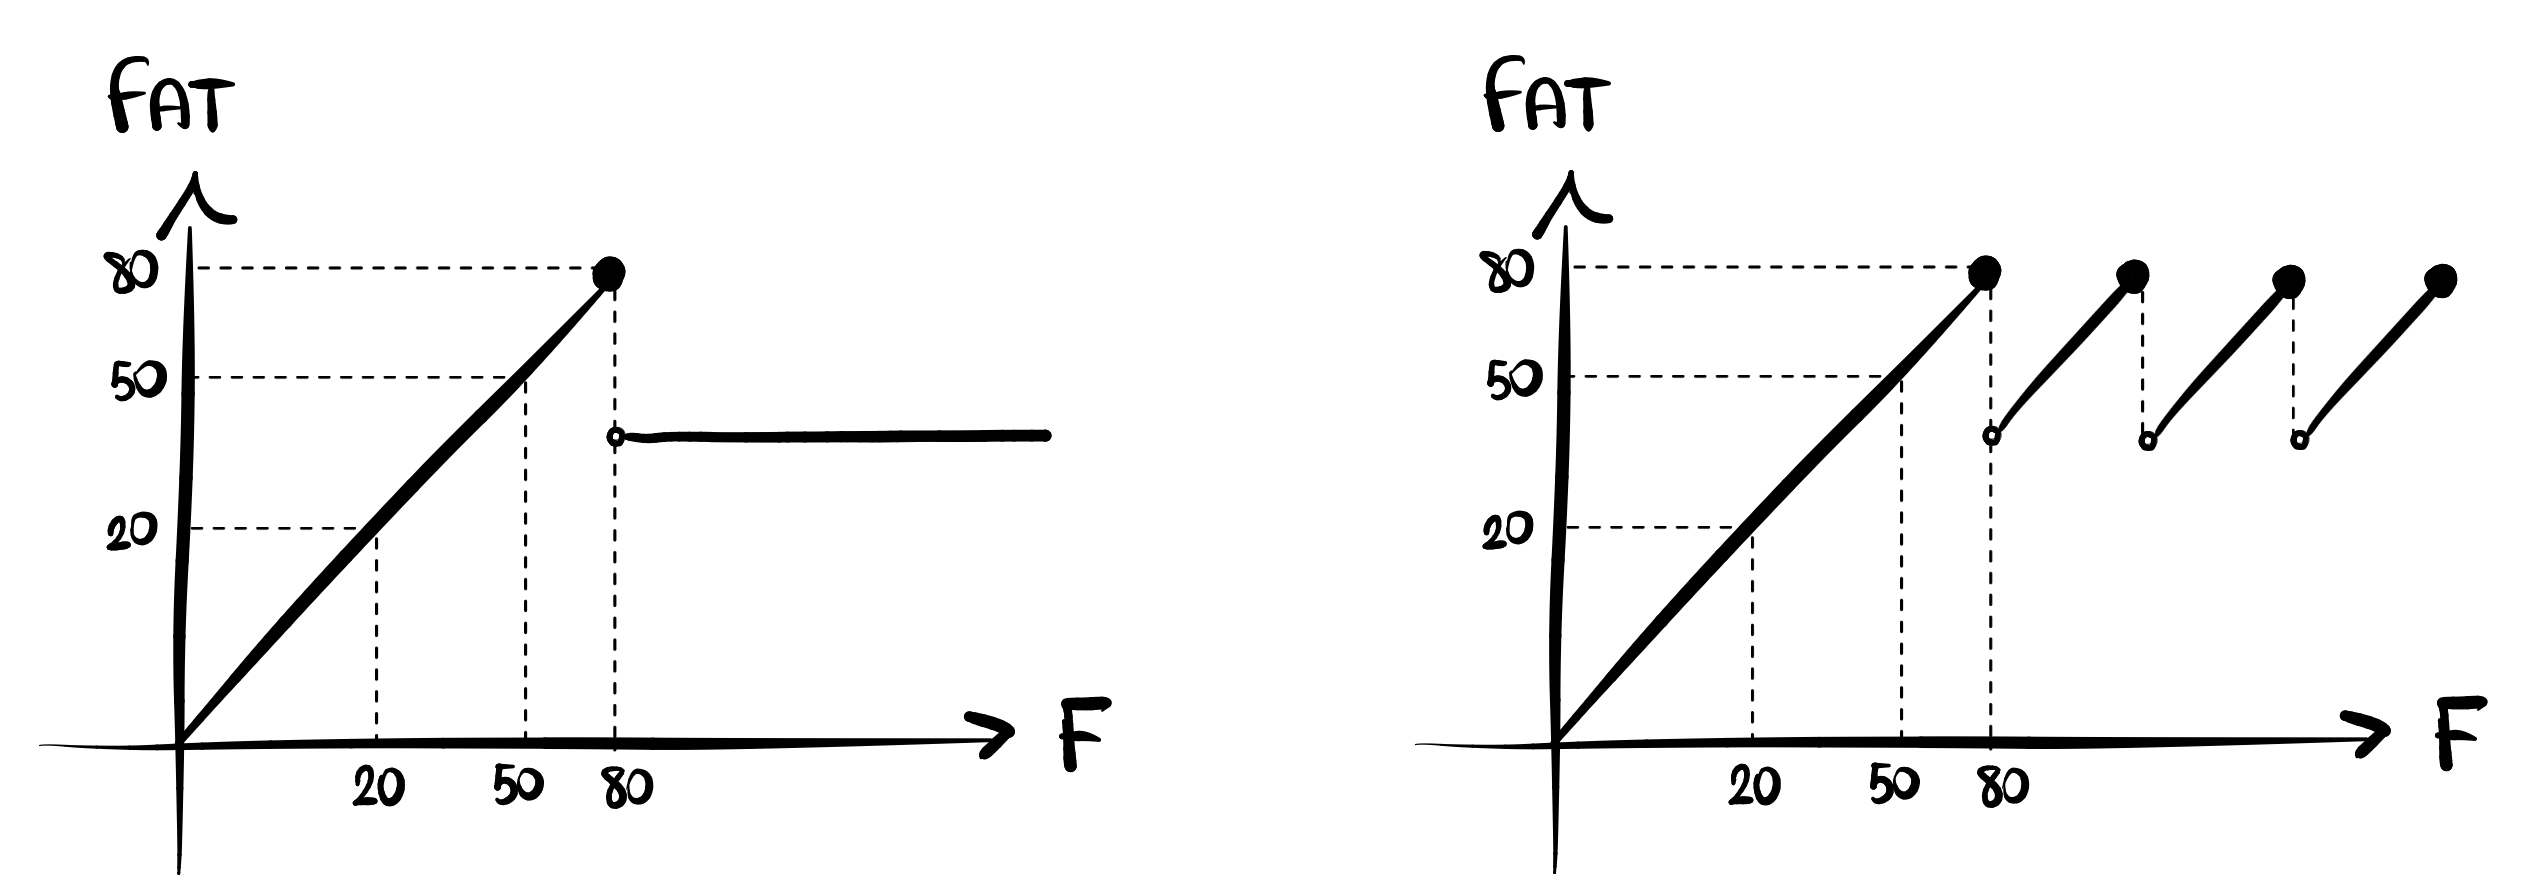
\includegraphics[width=0.8\linewidth]{imagensdinamicanewton/fatABS.png}};
  \end{scope}
\end{tikzpicture}
\captionof{figure}{O carro sem freio ABS (primeira imagem) e com freio ABS (segunda imagem).}
\label{fig_mec_fatcABS}
} 
\vspace{0.3cm}







Já o sistema de freios ABS impede que a roda permaneça travada. Sensores monitoram continuamente a rotação das rodas e modulam a pressão do freio diversas vezes por segundo. O sistema permite que a força atinja valores próximos ao máximo estático e, antes que o deslizamento se estabeleça completamente, reduz momentaneamente a força aplicada, voltando em seguida a aumentá-la. Esse ciclo se repete rapidamente.

No gráfico, isso aparece como pequenas oscilações próximas ao valor máximo do atrito estático. O sistema mantém o funcionamento na região de maior aderência possível, escolhendo sempre o atrito estático no lugar do cinético, haja vista que $\mu_e \geq \mu_c.$


O ABS, portanto, não cria mais atrito. Ele apenas impede que o sistema entre no regime menos eficiente. Em termos físicos, ele mantém o contato pneu-solo operando próximo do atrito estático máximo em vez de permitir que a situação evolua para o regime de atrito cinético. Essa diferença -- que pode parecer apenas um detalhe de coeficientes -- é suficiente para reduzir significativamente a distância de frenagem e preservar a dirigibilidade.



% {
% \centering
% 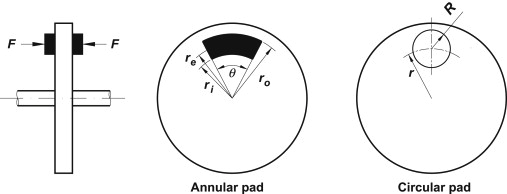
\includegraphics[width=0.7\linewidth]{imagensdinamicanewton/fatABS disco de freio.png}
% \captionof{figure}{A força de compressão do disco de freio.}
% \label{fig_mec_fatABS disco de freio}
% } 
% \vspace{0.3cm}








\secgfe{Erros comuns}

O erro mais comum aqui é confundir os tipos de atrito, e considerar, por exemplo, que a força de atrito cinético possui módulo variável. Portanto, cabe lembrar ao leitor: se há movimento relativo entre as superfícies, o atrito atuante será o cinético, cujo módulo é sempre constante e dado pela Equação \eqref{eq_newton_fatcinetico}. 

Tal valor independe da velocidade com que o bloco se move, da sua área de contato com o chão, etc.


\secgfe{Observações}

Algumas observações merecem ser pontuadas. A primeira delas se refere ao fato de que a força de atrito não depende da área de contato. Este é talvez o resultado mais contraintuitivo da teoria do atrito, e foi enunciado por Guillaume Amontons em 1699 — quase oitenta anos
antes de Coulomb sistematizar a teoria.

Um bloco com face larga em contato com o chão experimenta
\emph{a mesma} força de atrito que o mesmo bloco apoiado sobre sua
face estreita, desde que a força normal seja igual nos dois casos.
A explicação microscópica é a seguinte: uma área maior distribui o
peso por mais pontos de contato, reduzindo a pressão em cada um;
uma área menor concentra o peso em menos pontos, aumentando a pressão
local.
Os dois efeitos se compensam exatamente, e o atrito total permanece
o mesmo. É por isso que a fórmula $F_\text{AT} = \mu_c N$ não contém nenhum
termo de área.

Outra observação é sobre o fato de que a força de atrito não depende (aproximadamente) da velocidade.
Dentro de uma faixa razoável de velocidades — que abrange praticamente
todas as situações do Ensino Médio e da engenharia cotidiana —,
$\mu_c$ é constante.
Um bloco deslizando a $1\ \text{m/s}$ experimenta a mesma força de
atrito que o mesmo bloco deslizando a $10\ \text{m/s}$, sobre a mesma
superfície, com a mesma força normal.
Essa independência da velocidade é o terceiro pilar da lei de Coulomb
do atrito e justifica o uso de um único coeficiente $\mu_c$ em todos
os problemas de deslizamento.
As situações em que essa aproximação falha — superfícies lubrificadas,
velocidades muito altas, materiais muito macios como borracha —
chamamos de regime de atrito viscoso ou atrito de Stribeck,
e o estudo delas pertence à tribologia, a ciência das superfícies
em contato.

A tabela abaixo reúne valores representativos para pares de materiais
comuns.
Todos são adimensionais e valem para superfícies secas e limpas,
a menos que indicado.

\begin{center}
\begin{tabular}{lc}
\hline
\textbf{Par de materiais} & $\boldsymbol{\mu_c}$ \textbf{aproximado} \\
\hline
Borracha sobre asfalto seco & $0{,}7$ \\
Aço sobre aço               & $0{,}4$ a $0{,}6$ \\
Madeira sobre madeira       & $0{,}2$ a $0{,}5$ \\
Gelo sobre gelo             & $0{,}03$ \\
Teflon sobre aço            & $0{,}04$ \\
\hline
\end{tabular}
\end{center}


\vspace{0.3cm}

\begin{exemplo}[Nível I]\label{exemplo_newton_fatcinetico01}

Considere a situação da Figura \ref{fig_mec_fatcineticografico}, em que o bloco de massa $m=4$kg se move com velocidade $v_0=12$ m/s no instante inicial, sem nenhuma força o empurrando no sentido do seu movimento. Se a superfície de contato entre o bloco e o solo é horizontal, e os coeficientes de atrito são $\mu_e=0.6$ e $\mu_c = 0.3,$ calcule a distância percorrida pelo bloco até que ele pare.

\resolucao

Se o bloco se move com velocidade $v_0=12$ m/s já sabemos, de antemão, que há movimento relativo entre as superfícies em questão (bloco e chão), de modo que o atrito que atua é o atrito cinético. A Figura \ref{fig_mec_fatcineticoex01} mostram as forças que atuam no bloco.


\vspace{0.3cm}
{
\centering
\begin{tikzpicture}
  \begin{scope}[blend mode=multiply]
    \node {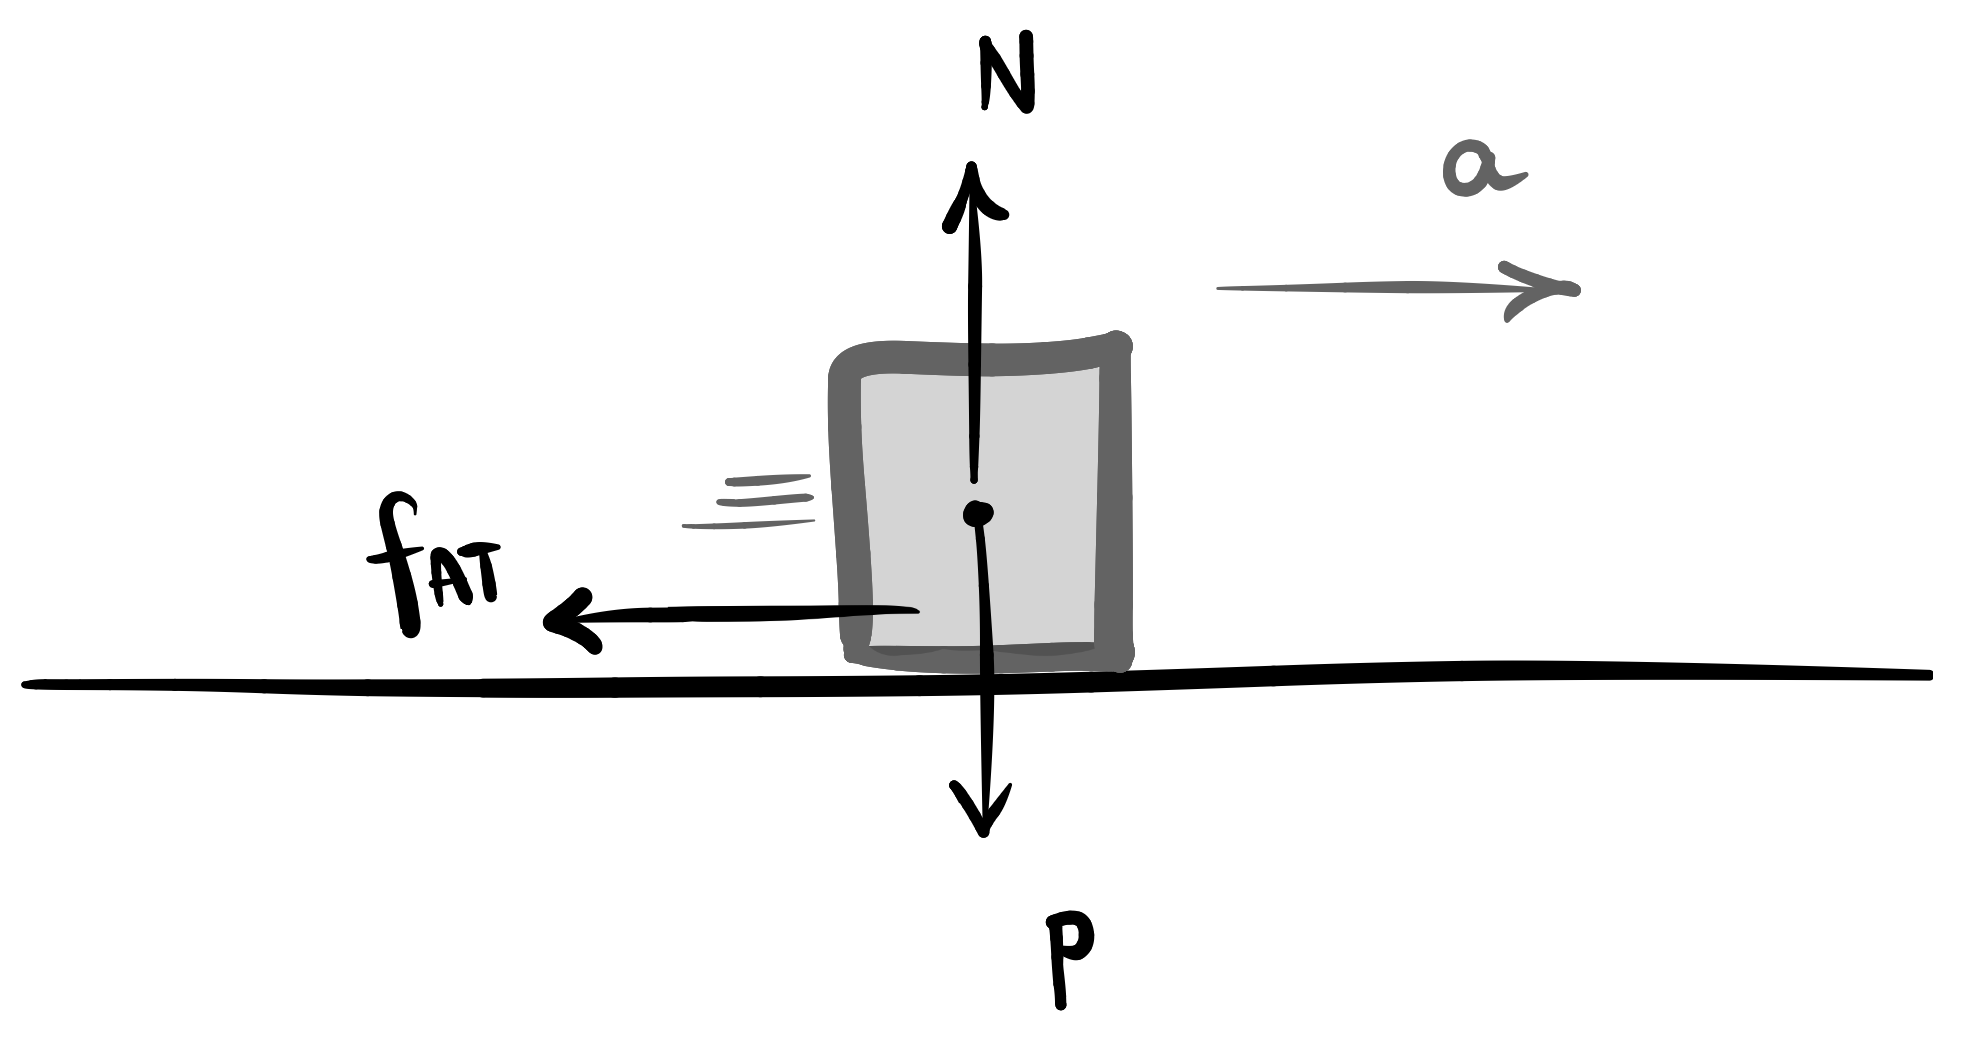
\includegraphics[width=0.4\linewidth]{imagensdinamicanewton/fatcineticoex01.png}};
  \end{scope}
\end{tikzpicture}
\captionof{figure}{}
\label{fig_mec_fatcineticoex01}
} 
\vspace{0.3cm}


Na vertical há equilíbrio, logo, temos

$$ F_{Ry}=0 \implies N = P=mg.$$

Na horizontal, pela Segunda lei de Newton, teremos

$$ F_{Rx} = ma_x \implies F_{AT_{C}} =ma_x,$$

\noindent e, pela Equação \eqref{eq_newton_fatcinetico}, teremos

$$ F_{AT_{C}} =ma_x \implies \mu_c mg = m a_x \implies a_x = \mu_c g = 0.3 \cdot 10 \implies \boxed{a_x = 3 \text{m/s}^2.} $$

Logo, o bloco se move em um MUV, com velocidade inicial $v_0=12$ e uma desaceleração $a=3 \text{m/s}^2.$ Podemos, portanto, usar a Equação de Torricelli para resolver o problema:

$$ \cancelto{0}{v^2} = v_0^2 - 2 a \Delta s \implies \Delta s = \dfrac{v_0^2}{2a} = \dfrac{12^2}{2 \cdot 3} \implies \boxed{\Delta s = 24 \text{ m}.} $$

\end{exemplo}


\vspace{0.3cm}

\begin{exemplo}[Nível II]\label{exemplo_newton_fatcinetico02}

Um bloco de $4{,}0\ \text{kg}$ repousa sobre um plano inclinado de
$30°$. Os coeficientes de atrito estático e cinético entre o bloco
e o plano valem $\mu_e = 0{,}60$ e $\mu_c = 0{,}40$. Determine se
o bloco desce espontaneamente e, caso desça, calcule sua aceleração.
Use $g = 10\ \text{m/s}^2$.


\resolucao


No plano inclinado, a força que tende a provocar o deslizamento é a componente do peso ao longo do plano. A pergunta ``o bloco se move?'' torna-se: ``a componente do
peso ao longo do plano supera o atrito estático máximo?''

A força normal é:
\[
  N = mg\cos 30^\circ = 4{,}0 \cdot 10 \cdot \frac{\sqrt{3}}{2}
  \approx 34{,}6\ \text{N}.
\]
A componente do peso ao longo do plano (para baixo) é:
\[
  P_{//} = mg\,\sin  30^\circ = 4{,}0 \cdot 10 \cdot 0{,}50
  = 20\ \text{N}.
\]
O atrito estático máximo (que se oporia ao deslizamento, portanto
para cima do plano) é:
\[
  F_{\text{AT}_{MAX}} = \mu_e N = 0{,}60 \cdot 34{,}6
  \approx 20{,}8\ \text{N}.
\]

Como $P_{//} = 20 <20{,}8\
\text{N}$, o atrito estático consegue segurar o bloco.
O bloco permanece em repouso sobre o plano — e a força de atrito
que efetivamente atua é $20\ \text{N}$ (igual e oposta a
$P_{//}$), não o valor máximo de $20{,}8\ \text{N}$.

Se o coeficiente estático fosse ligeiramente menor — digamos
$\mu_e = 0{,}55$, dando $F_{\text{AT}_{MAX}} = 19\ \text{N}$ —,
o peso ao longo do plano venceria o atrito estático máximo e o bloco deslizaria.
Nesse caso, a aceleração seria calculada com $\mu_c$:
\[
  a = g\left(\sin 30^\circ - \mu_c\cos 30^\circ \right)
  = 10\!\left(0{,}50 - 0{,}40\cdot\frac{\sqrt{3}}{2}\right)
  \approx 10\,(0{,}50 - 0{,}35)
  = 1{,}5\ \text{m/s}^2.
\]

Perceba que o atrito cinético só é convocado \emph{depois} de
confirmado que o objeto desliza. O diagnóstico correto — estático ou cinético? — é sempre o primeiro passo, e ele depende de comparar a força motriz com
$F_{\text{AT}_{MAX}} = \mu_e N$, não com $\mu_c N$.


\end{exemplo}


\vspace{0.3cm}



\begin{exemplo}[Nível III (ITA - 1997)]\label{exemplo_newton_fatcinetico03}




Um antigo vaso chinês está a uma distância $d$ da extremidade de um forro, sobre uma mesa fixa ao solo. Essa extremidade, por sua vez, encontra-se a uma distância $D$ de uma das bordas da mesa, como mostra a figura. Você apostou que consegue puxar o forro da mesa com uma aceleração $a$, de tal forma que o vaso não caia da mesa. 

\vspace{0.3cm}
{
\centering
\begin{tikzpicture}
  \begin{scope}[blend mode=multiply]
    \node {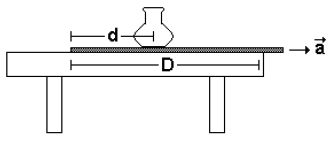
\includegraphics[width=0.4\linewidth]{imagensdinamicanewton/vaso chines.png}};
  \end{scope}
\end{tikzpicture}
\captionof{figure}{}
\label{fig_mec_vasochinesITA}
} 
\vspace{0.3cm}

Considere que ambos os coeficientes de atrito, cinético e estático, entre o vaso e o forro tenham valor $\mu$, e que o vaso pare ao tocar a mesa. Você ganhará a aposta se a intensidade da aceleração $a$ estiver dentro da faixa:

\begin{enumerate}
\item [a)] $a < \dfrac{d\,\mu\,g}{D}$
\item [b)] $a > \dfrac{d\,\mu\,g}{D}$
\item [c)] $a > \mu g$
\item [d)] $a > \dfrac{D\,\mu\,g}{d}$
\item [e)] $a > \dfrac{D\,\mu\,g}{D-d}$
\end{enumerate}


\resolucao


Considerando um sistema de coordenadas orientado para a direita com origem na extremidade esquerda do forro, a função de posição para a extremidade esquerda do forro é

$$s_f = \dfrac{1}{2}at^2.$$

A extremidade esquerda do forro alcança a borda da mesa (ou seja, o forro é totalmente retirado da mesa) em $s=D.$ Chamemos de $t_1$ o instante em que isso ocorre:

$$ s_f = \dfrac{1}{2}at^2 = D \implies t_1 = \sqrt{\dfrac{2D}{a}}. $$

Venceremos a aposta caso o vaso demore mais tempo para alcançar essa mesma posição -- o que significa que conseguimos puxar o forro totalmente antes do vaso alcançar a borda. 

\medskip

O vaso, que escorrega ao longo do forro, está em regime de atrito cinético (coeficiente $\mu$). Sendo a normal igual ao seu peso (equilíbrio de forças na vertical), a força de atrito é

$$F_{\text{AT}_{CIN}} = \mu N = \mu mg,$$

\noindent de modo que aceleração do vaso $a'$ é, portanto:
$$F_{\text{AT}_{CIN}} = ma' \implies ma' = \mu m g \implies  a' = \mu g.$$ 
 
A função horária da posição para o vaso é

$$s_v= d+\dfrac{1}{2} \mu gt^2,$$

\noindent e ele alcança a posição $s=D$ no instante $t_2$ dado por


$$s_v= d+\dfrac{1}{2} \mu gt^2 = D \implies t_2 = \sqrt{\dfrac{2(D-d)}{\mu g}}. $$

Como dito, precisamos que $t_2 > t_1,$ ou seja, o vaso leva mais tempo para alcançar a borda da mesa do que o forro:

$$ \sqrt{\dfrac{2(D-d)}{\mu g}} > \sqrt{\dfrac{2D}{a}},$$

\noindent o que nos leva a

$$ \boxed{a > \dfrac{\mu g D}{D-d} \implies \text{ letra E.}}$$

\end{exemplo}




\begin{secnivel}[Força de Resistência do Ar]{II}{Força de Resistência do Ar}
  
  \eqLdois{exp}{eq_newton_forcaresistenciaar}{F_{\text{RAR}}=\dfrac{1}{2}C\rho Av^2}

\end{secnivel}




Essa equação representa a força de resistência que um corpo sente ao se deslocar através de um fluido\footnote{Fluidos podem ser gases ou líquidos. Desse modo, o que estudaremos aqui não valerá apenas para o ar -- apesar de este ser o caso mais comum de se estudar. Vale para um submarino se movendo em um oceano, por exemplo. A resistência que ele sentiria ao seu movimento seria de mesma natureza daquela que estudaremos aqui. A força, neste caso, receberia o nome de força de arrasto.} de densidade $\rho.$ Em tal equação $v$ é a velocidade com que o corpo se move \footnote{Como veremos em alguns exemplos, a força de arrasto pode ser proporcional à velocidade ou ao quadrado da velocidade. Dizemos, no primeiro caso, que temos um regime linear e, no segundo, um regime quadrático. De modo geral é possível ter a força dependendo das duas potências, isto é, $F_{\text{RAR}
}(v) = av + bv^2$, em que $a$ e $b$ são constantes. Contudo, para o tratamento que aqui faremos, a expressão da Equação \eqref{eq_newton_forcaresistenciaar} será suficiente para que consigamos extrair o caráter qualitativo a respeito do movimento de um corpo sob ação da força de arrasto.},  $A$ é a sua área de seção transversal e $C$ é o chamado coeficiente de arrasto.




\secgfe{De onde vem}


Quando um corpo se move através de um fluido --- seja o ar, seja a água --- as moléculas desse fluido estão, do ponto de vista do corpo, vindo em sua direção. O corpo precisa continuamente afastá-las, empurrá-las para os lados, abrir caminho. Esse trabalho coletivo de deslocar o fluido tem um custo: o fluido reage empurrando o corpo de volta, na direção oposta ao movimento. É essa reação do meio que chamamos de força de resistência, ou arrasto.

A intensidade dessa força depende, intuitivamente, de quatro coisas: de quão denso é o fluido, de quão grande é a ``silhueta'' que o corpo apresenta ao escoamento, de quão rápido ele se move e de quão aerodinâmico é  seu formato. A Equação \eqref{eq_newton_forcaresistenciaar} é uma relação obtida experimentalmente e sintetiza essas quatro intuições. Vejamos cada um em detalhes.

\subsubsection*{Os fatores da equação}

A \textit{densidade} $\rho$ entra porque fluidos mais densos opõem mais resistência. Nadar em água exige esforço incomparavelmente maior do que caminhar no ar à mesma velocidade, e o fator $\approx 800$ entre as densidades da água e do ar explica boa parte disso. Mais massa por volume significa mais matéria a ser deslocada a cada instante.

A \textit{área de seção transversal} $A$ entra porque um corpo de frente larga intercepta mais fluido do que um perfil estreito. Um caminhão e uma bicicleta percorrendo a mesma estrada à mesma velocidade sentem resistências muito diferentes --- e a diferença de área frontal é o principal culpado.

A \textit{velocidade} $v$ aparece ao quadrado na forma que usamos, embora valha registrar que isso não é universal: em regimes de escoamento muito lento --- gotas microscópicas sedimentando, objetos em fluidos muito viscosos --- a resistência cresce linearmente com $v$. Para as velocidades do cotidiano e do ensino médio, contudo, o regime quadrático é o relevante. De toda forma, como veremos, nosso interesse nessa equação no contexto do ensino médio é essencialmente qualitativo --- ela serve menos para calcular do que para entender como cada fator influencia o arrasto. A dependência exata em $v$ importa pouco nesse horizonte. Contudo, é evidente que, quanto maior for a velocidade de um corpo, mais intensos serão os choques que ele sofrerá contra as moléculas do fluido, de modo que mais intensa será a força de resistência sentida por ele.

O \textit{coeficiente de arrasto} $C$ é o ingrediente que encapsula tudo aquilo que a forma do objeto e as complexidades do escoamento determinam e que não pode ser calculado a partir de primeiros princípios. Vamos discutir melhor o seu significado na seção \emph{Observações} sobre esta equação.

O fator $\sfrac{1}{2}$, por fim, é uma convenção, cuja razão de ser envolve detalhes técnicos que fogem do escopo deste livro.






\secgfe{Onde é usada}

A Equação \eqref{eq_newton_forcaresistenciaar} dificilmente será usada de forma direta no contexto do Ensino Médio. Isso porque uma força que depende da velocidade gera um problema matemático um tanto quanto complexo. Perceba que a força é o que faz variar a velocidade $v$, isto é, ela gera aceleração. Porém, a força $F_{\text{RAR}}$ depende também do valor da velocidade $v$, ou seja, a força afeta a velocidade (gerando aceleração), porém, a alteração da velocidade irá afetar o próprio valor da força. Sendo assim, a ação da força sob o corpo irá gerar um efeito que fará a própria força mudar de valor.

Isso é o que gera toda a complexidade em tratar, matematicamente, de uma força como essa. Seria preciso o conhecimento da solução de equações diferenciais para aplicar de forma direta a Equação \eqref{eq_newton_forcaresistenciaar}, o que foge do escopo do Ensino Médio. Sendo assim, o mais interessante é sabermos extrair informações qualitativas a respeito do que tal equação implica em alguns contextos, como veremos em breve.


\secgfe{Erros comuns}

São poucos os problemas em que levaremos em consideração a resistência do ar. Porém, nesses poucos casos, o erro mais comum é o estudante não perceber que força de resistência do ar pode variar por diversos motivos, sendo o mais comum deles:

\begin{enumerate}
    \item [(i)] a variação da velocidade $v$ da partícula: se a velocidade aumentar, a força de resistência do ar será maior; se ela diminuir, a força de resistência do ar será menor.

    \item [(ii)] a variação da área superficial frontal $A$ do corpo.
\end{enumerate}

Considere, por exemplo, a situação de uma pedra, abandonada do repouso em queda livre, em que há resistência do ar.

Ora, como a pedra começa do repouso, temos que $v_0=0,$ de modo que a força de resistência do ar $F_{\text{RAR}}$ é, inicialmente, nulo. Contudo, à medida que a pedra é acelerada pela gravidade, ela começa a ganhar velocidade, de modo que, pela Equação \eqref{eq_newton_forcaresistenciaar}, começa a surgir uma força de resistência do ar. A Figura \ref{fig_mec_frarqueda1} ilustra tal situação: a partícula parte do repouso, situação na qual a força resultante que atua sob ela é igual ao seu peso.

\vspace{0.3cm}
{
\centering
\begin{tikzpicture}
  \begin{scope}[blend mode=multiply]
    \node {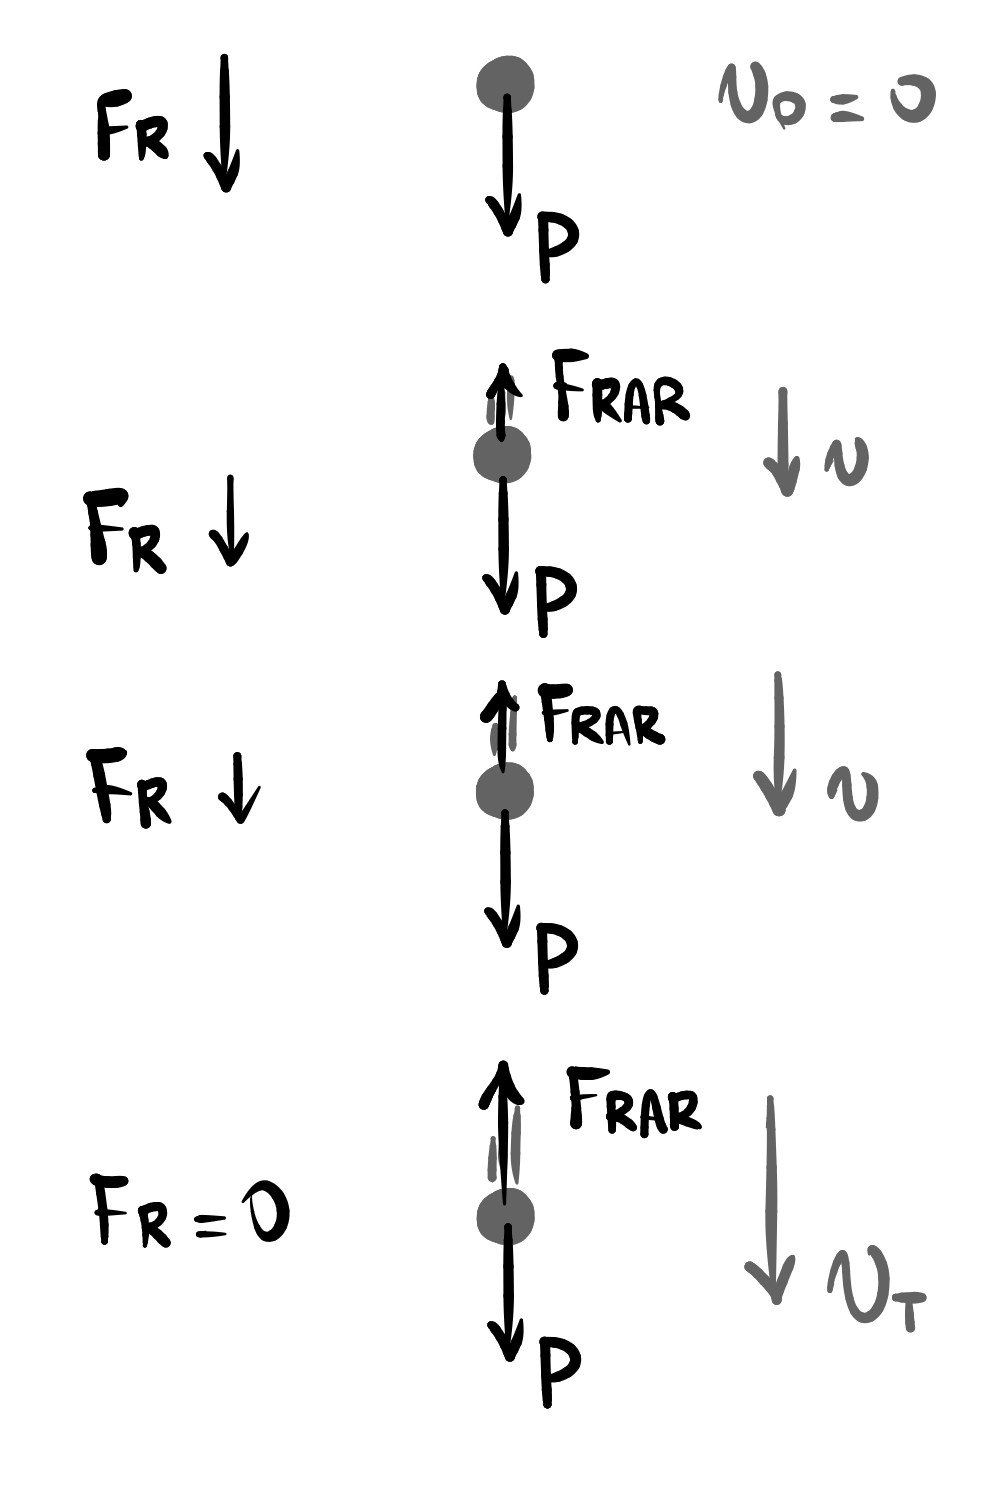
\includegraphics[width=0.25\linewidth]{imagensdinamicanewton/frarqueda1.png}};
  \end{scope}
\end{tikzpicture}
\captionof{figure}{}
\label{fig_mec_frarqueda1}
} 
\vspace{0.3cm}

À medida que ela começa a ganhar velocidade, começa a surgir a força de resistência do ar, que se opõe ao seu movimento. Tal força, contudo, começa pequena, de modo que a força resultante continua para baixo, ou seja, a partícula continua em movimento acelerado. Contudo, quanto mais sua velocidade aumenta, maior se torna a força de resistência do ar, de modo que a força resultante vai diminuindo -- a partícula vai ganhando cada vez menos velocidade. Em certo momento, a força de resistência do ar cresceu a ponto de se igualar ao peso: neste ponto, a força resultante é zero. Sendo assim, a partícula começa a se mover em movimento uniforme -- a velocidade sendo constante faz com que a força de resistência do ar seja, também, constante, como diz a Equação \eqref{eq_newton_forcaresistenciaar} -- trata-se de uma condição de \emph{equilíbrio dinâmico.} 




Dizemos que neste ponto a partícula atingiu a \emph{velocidade terminal} $v_{\text{T}}:$ a partir daqui ela não acelera mais, haja vista que a força de resistência do ar se tornou capaz de anular o peso. Daqui em diante o movimento passa a ser uniforme. É possível, com facilidade, computar o valor da velocidade terminal. É aquele para o qual a força resultante é zero:

$$ F_{\text{R}} =0 \implies F_{\text{RAR}}= P \implies \dfrac{1}{2}C\rho Av_{\text{T}}^2 = mg \implies \boxed{v_{\text{T}}= \sqrt{\dfrac{2mg}{C \rho A}}.}$$

Tal valor de velocidade é representado pela linha pontilhada do segundo gráfico da Figura \ref{fig_mec_frarqueda2}: a velocidade começa nula e aumenta exponencialmente\footnote{A explicação de por que a curva é exatamente uma exponencial envolve a parte matemática mais complicada anteriormente citada,} até atingir a velocidade terminal.

A primeira imagem do gráfico mostra também o que ocorre com a força resultante sob a partícula: ela começa sendo exatamente igual ao seu peso, diminuindo também exponencialmente até zerar, ponto no qual a partícula atinge a velocidade terminal.


\vspace{0.3cm}
{
\centering
\begin{tikzpicture}
  \begin{scope}[blend mode=multiply]
    \node {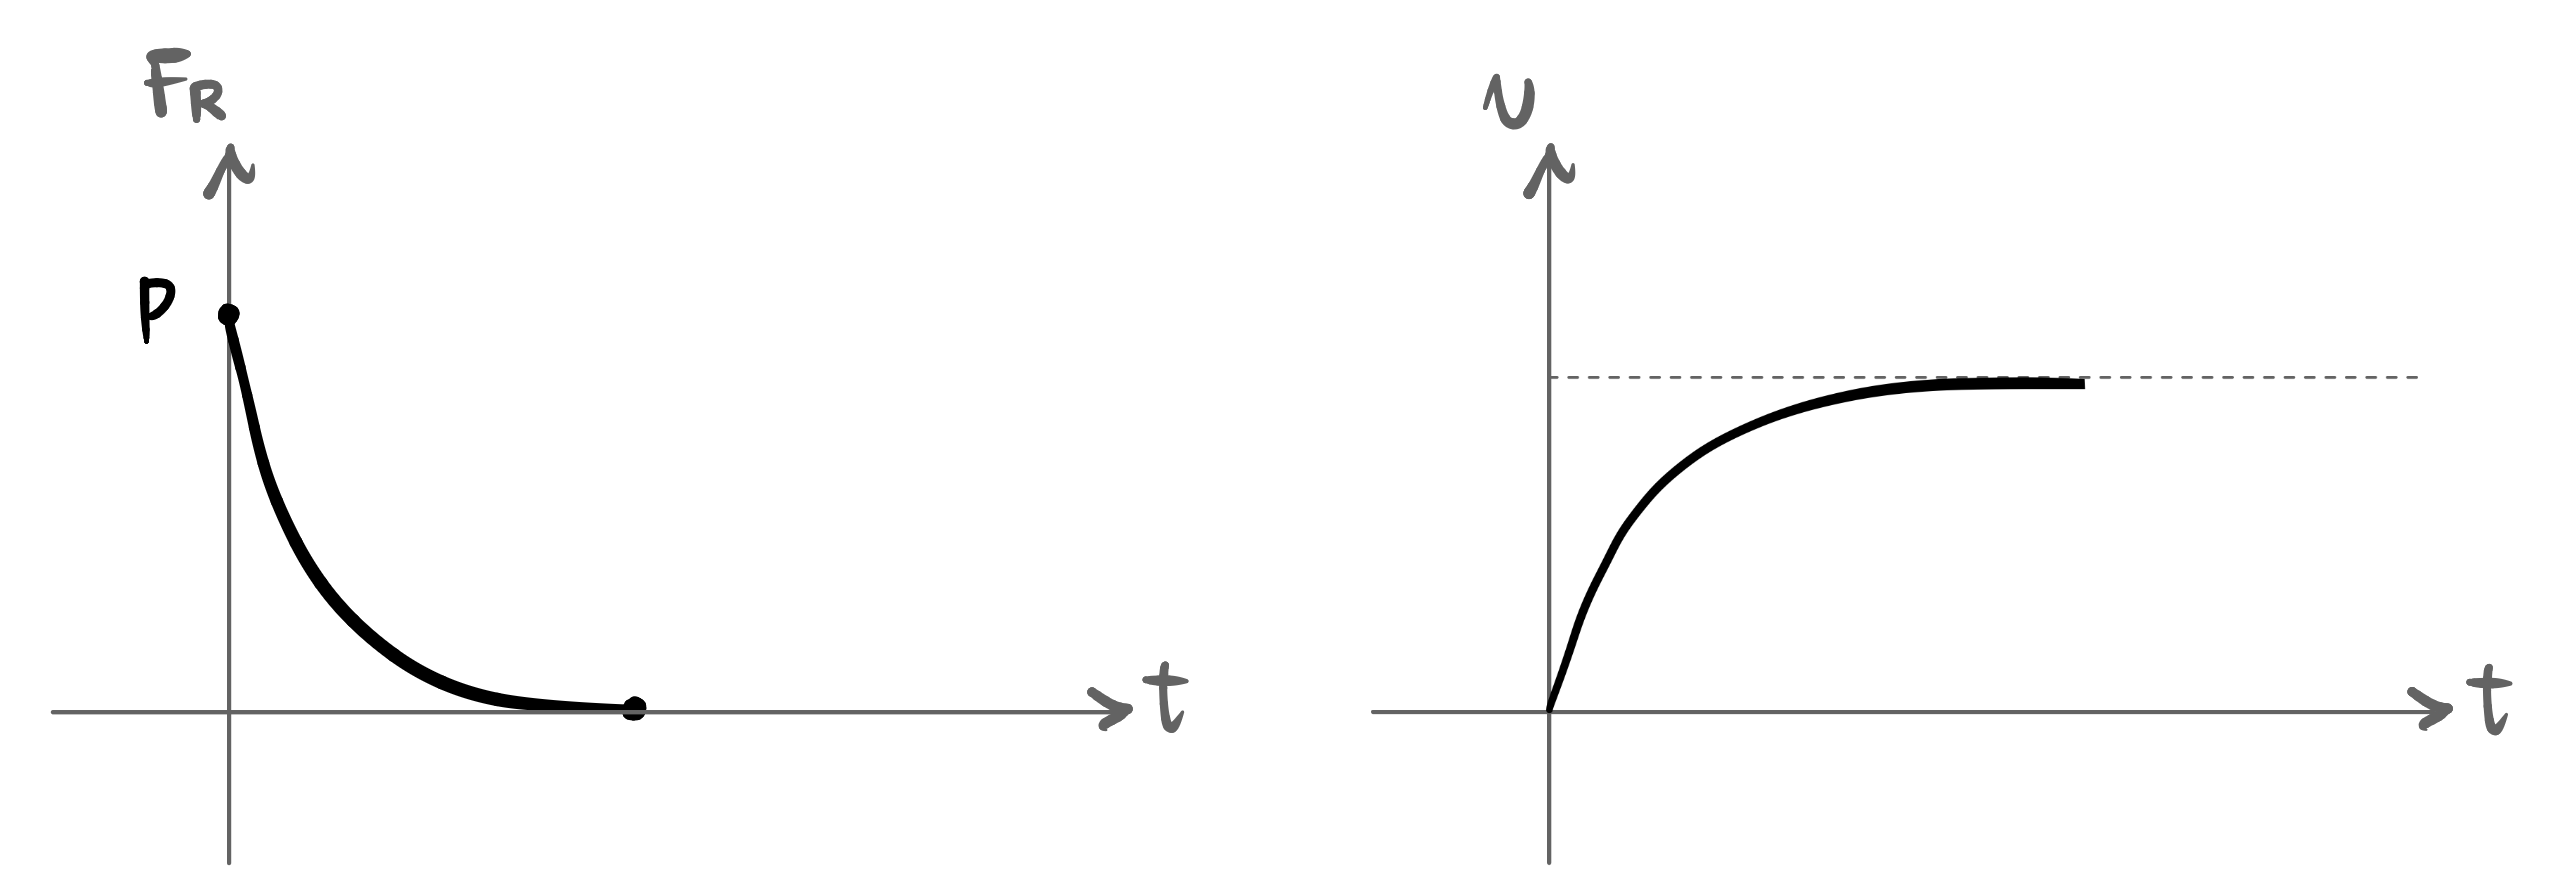
\includegraphics[width=0.8\linewidth]{imagensdinamicanewton/frarqueda2.png}};
  \end{scope}
\end{tikzpicture}
\captionof{figure}{Gráficos da força resultante $F_{\text{R}}$ e da velocidade $v$ da partícula em função do tempo.}
\label{fig_mec_frarqueda2}
} 
\vspace{0.3cm}



\secgfe{Observações}

É possível que se tenha dois corpos de mesma área da seção transversal $A$, imersos em um mesmo fluido de densidade $\rho$ e se movendo a uma mesma velocidade $v$, porém, ainda assim, sofrendo diferentes forças de resistência do ar. Tal situação está representada na Figura \ref{fig_mec_arrastoar}.

\vspace{0.4cm}
{
\centering
\begin{tikzpicture}
  \begin{scope}[blend mode=multiply]
    \node {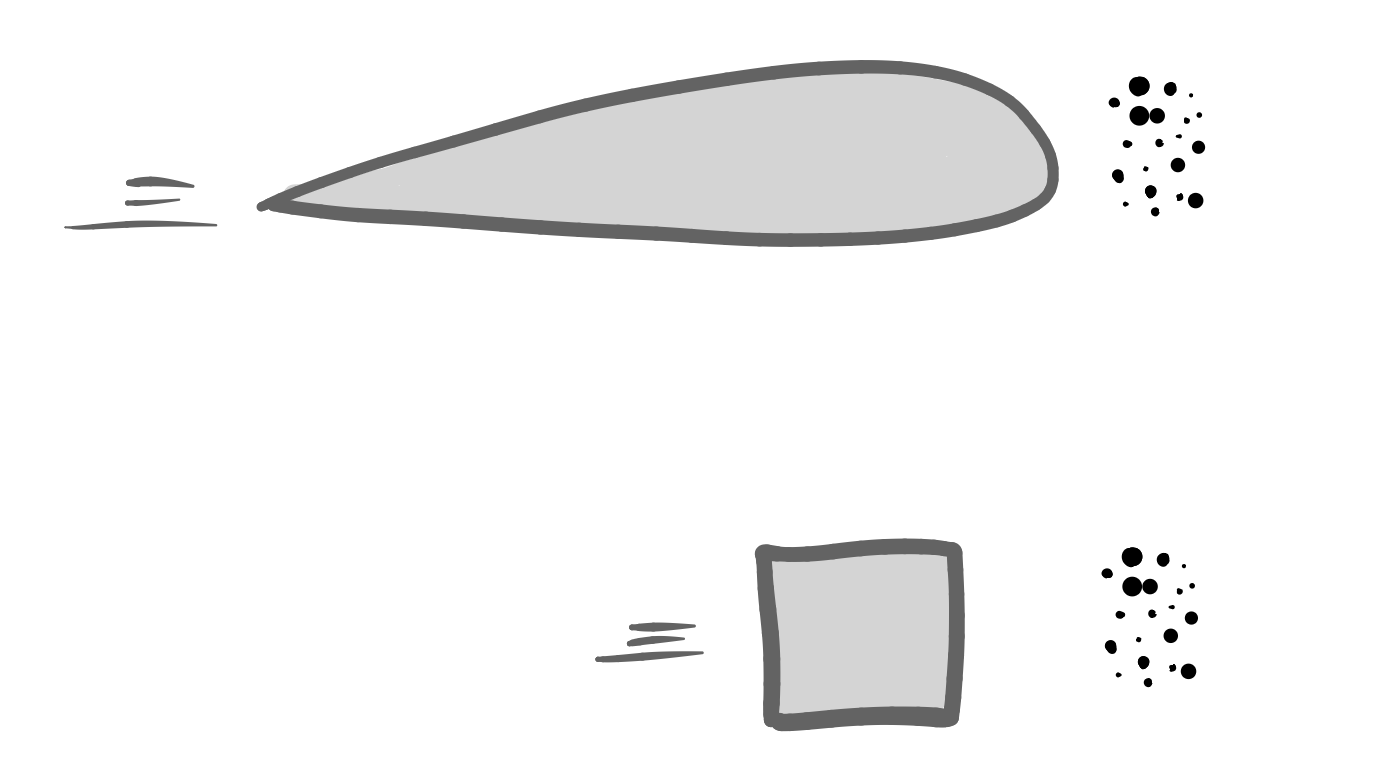
\includegraphics[width=0.35\linewidth]{imagensdinamicanewton/arrastoar.png}};
  \end{scope}
\end{tikzpicture}
\captionof{figure}{A aerodinâmica dos corpos influencia na força de arrasto.}
\label{fig_mec_arrastoar}
} 
\vspace{0.3cm}

Note que, apesar da área seção transversal ser a mesma -- o que significa que a parte frontal dos dois corpos irá esbarrar com mesma quantidade de ar -- e de terem a mesma velocidade -- o que quer dizer que o choque dos dois corpos com as partículas do ar terá a mesma intensidade -- existe um formato geométrico em que o ar consegue \textit{escorregar} com mais facilidade através do corpo, o que fará a força de resistência ser menor. Dizemos que a aerodinâmica de tal corpo é melhor: trata-se de um formato geométrico que possibilita que o ar escoe com menos resistência através do corpo. 

Tal característica é representada pelo coeficiente de arrasto $C$ na Equação \eqref{eq_newton_forcaresistenciaar}. 


\vspace{0.3cm}


\begin{exemplo}[Nível I (UFRS)]\label{exemplo_newton_frarex01}

Selecione a alternativa que preenche corretamente as lacunas do texto abaixo, 
na ordem em que elas aparecem. \\

Na sua queda em direção ao solo, uma gota de chuva sofre o efeito da resistência do ar. 
Essa força de atrito é contrária ao movimento e aumenta com a velocidade da gota. 
No trecho inicial da queda, quando a velocidade da gota é pequena e a resistência 
do ar também, a gota está animada de um movimento \underline{\hspace{1cm}}. 
Em um instante posterior, a resultante das forças exercidas sobre a gota torna-se nula. 
Esse equilíbrio de forças ocorre quando a velocidade da gota atinge o valor que torna 
a força de resistência do ar igual, em módulo, \underline{\hspace{2cm}} da gota. 
A partir desse instante, a gota \underline{\hspace{2cm}}.

\begin{enumerate}
\item [a)] acelerado – ao peso – cai com velocidade constante
\item [b)] uniforme – à aceleração – cai com velocidade decrescente
\item [c)] acelerado – ao peso – pára de cair
\item [d)] uniforme – à aceleração – pára de cair
\end{enumerate}


\resolucao

O contexto aqui é idêntico ao da pedra em queda, cujos gráficos estão representados na Figura \ref{fig_mec_frarqueda2}. Como vimos, o movimento é inicialmente \textbf{acelerado}, até que a força de resistência cresce o suficiente a ponto de \textbf{igualar ao peso} da gota, situação na qual o movimento passa a ser com \textbf{velocidade} constante, ou seja, um movimento uniforme.

Desse modo a resposta é a alternativa $(a).$

\end{exemplo}


\vspace{0.3cm}


\begin{exemplo}[Nível II (ENEM - 2013)]\label{exemplo_newton_frarex02}

Em um dia sem vento, ao saltar de um avião, um paraquedista cai verticalmente 
até atingir a velocidade limite. No instante em que o paraquedas é aberto 
(instante $T_A$), ocorre a diminuição de sua velocidade de queda. Algum tempo 
após a abertura do paraquedas, ele passa a ter velocidade de queda constante, 
o que possibilita sua aterrissagem em segurança.

Que gráfico representa a força resultante sobre o paraquedista, durante o seu 
movimento de queda?



\begin{tabular}{r m{5.5cm} r m{5.5cm}}

  a) &
  \begin{tikzpicture}[scale=0.41]
    \draw[->] (-0.3, 0) -- (5.5, 0) node[right] {\small Tempo};
    \draw[->] (0, -3.2) -- (0, 4.2) node[above, align=center] {\small Força\\\small resultante};
    \node[below left] at (0,0) {$0$};
    \draw[thick] plot[smooth] coordinates {
      (0.12,4.0)(0.3,3.1)(0.6,2.2)(1.0,1.4)
      (1.5,0.75)(2.0,0.35)(2.5,0.12)(2.85,0.02)};
    \draw[thick] plot[smooth] coordinates {
      (3.15,-3.0)(3.4,-1.8)(3.7,-1.0)(4.1,-0.5)
      (4.5,-0.22)(5.0,-0.08)(5.3,-0.03)};
    \draw[densely dotted, thick] (3.0,-3.2) -- (3.0,3.5);
    \node[below right] at (2.0,0) {$T_A$};
  \end{tikzpicture}

  & b) &

  \begin{tikzpicture}[scale=0.41]
    \draw[->] (-0.3, 0) -- (5.5, 0) node[right] {\small Tempo};
    \draw[->] (0, -3.2) -- (0, 4.2) node[above, align=center] {\small Força\\\small resultante};
    \node[below left] at (0,0) {$0$};
    \draw[thick] (0, 0)
      .. controls (0.06, 3.86) and (1.5, 3.86) .. (2.6, 3.8);
    \draw[thick] (2.6, 3.8)
      .. controls (2.8, 2.5) and (3.2, 1.2) .. (3.7, 0.5)
      .. controls (4.06, 0.1) and (4.4, 0.02) .. (4.9, 0.01);
    \draw[densely dotted, thick] (2.6, -3.2) -- (2.6, 3.8);
    \node[below] at (2.6, 0) {$T_A$};
  \end{tikzpicture} \\[6pt]

  c) &
  \begin{tikzpicture}[scale=0.41]
    \draw[->] (-0.3, 0) -- (5.5, 0) node[right] {\small Tempo};
    \draw[->] (0, -0.3) -- (0, 4.2) node[above, align=center] {\small Força\\\small resultante};
    \node[below left] at (0,0) {$0$};
    \draw[thick] (0, 4.1)
      .. controls (0.3, 0.02) and (1.8, 0.02) .. (3.0, 0.03)
      .. controls (3.8, 0.02) and (4.5, 0.01) .. (5.2, 0.005);
    \draw[densely dotted, thick] (3.0, 0) -- (3.0, 3.8);
    \node[below] at (3.0, 0) {$T_A$};
  \end{tikzpicture}

  & d) &

  \begin{tikzpicture}[scale=0.41]
    \draw[->] (-0.3, 0) -- (5.5, 0) node[right] {\small Tempo};
    \draw[->] (0, -0.3) -- (0, 4.2) node[above, align=center] {\small Força\\\small resultante};
    \node[below left] at (0,0) {$0$};
    \draw[thick] (0, 0)
      .. controls (0.05, 0) and (0.2, 1.7) .. (0.7, 2.8)
      .. controls (1.1, 3.5) and (1.7, 3.9) .. (2.5, 3.95)
      .. controls (3.2, 3.98) and (4.2, 3.99) .. (5.2, 3.99);
    \draw[densely dotted, thick] (2.5, 0) -- (2.5, 3.95);
    \node[below] at (2.5, 0) {$T_A$};
  \end{tikzpicture} \\[6pt]

  \multicolumn{4}{c}{e) \quad
 \begin{tikzpicture}[scale=0.41]
    \draw[->] (-0.3, 0) -- (5.5, 0) node[right] {\small Tempo};
    \draw[->] (0, -0.3) -- (0, 4.2) node[above, align=center] {\small Força\\\small resultante};
    \node[below left] at (0,0) {$0$};
    \draw[thick] (0, 0)
      .. controls (0.05, 0) and (0.2, 1.7) .. (0.7, 2.8)
      .. controls (1.1, 3.5) and (1.7, 3.9) .. (2.5, 3.95)
      .. controls (3.2, 3.98) and (4.2, 3.99) .. (5.2, 3.99);
    \draw[densely dotted, thick] (2.5, 0) -- (2.5, 3.95);
    \node[below] at (2.5, 0) {$T_A$};
  \end{tikzpicture}} \\




\end{tabular} 


\resolucao


A primeira parte do gráfico -- a queda até que se alcance a velocidade terminal -- já foi estudada por nós no movimento de queda da pedra, e o gráfico da força resultante por tempo aparece na primeira imagem da Figura \ref{fig_mec_frarqueda2}. Assim, as únicas alternativas cujo gráfico da primeira parte coincidem com aquele da Figura \ref{fig_mec_frarqueda2} são as letras $(a)$ e $(c)$.

\medskip

Vejamos o que ocorre a partir do instante $T_A,$ quando o indivíduo abre o paraquedas. O que acontece é que agora nós aumentamos o fator $A$ na Equação \eqref{eq_newton_forcaresistenciaar}: a área da seção frontal ficou maior, o que faz aumentar a força de resistência do ar haja vista que agora a colisão é contra um número muito maior de partículas de ar. A Figura \ref{fig_mec_paraquedas} ilustra isso.

\vspace{0.3cm}
{
\centering
\begin{tikzpicture}
  \begin{scope}[blend mode=multiply]
    \node {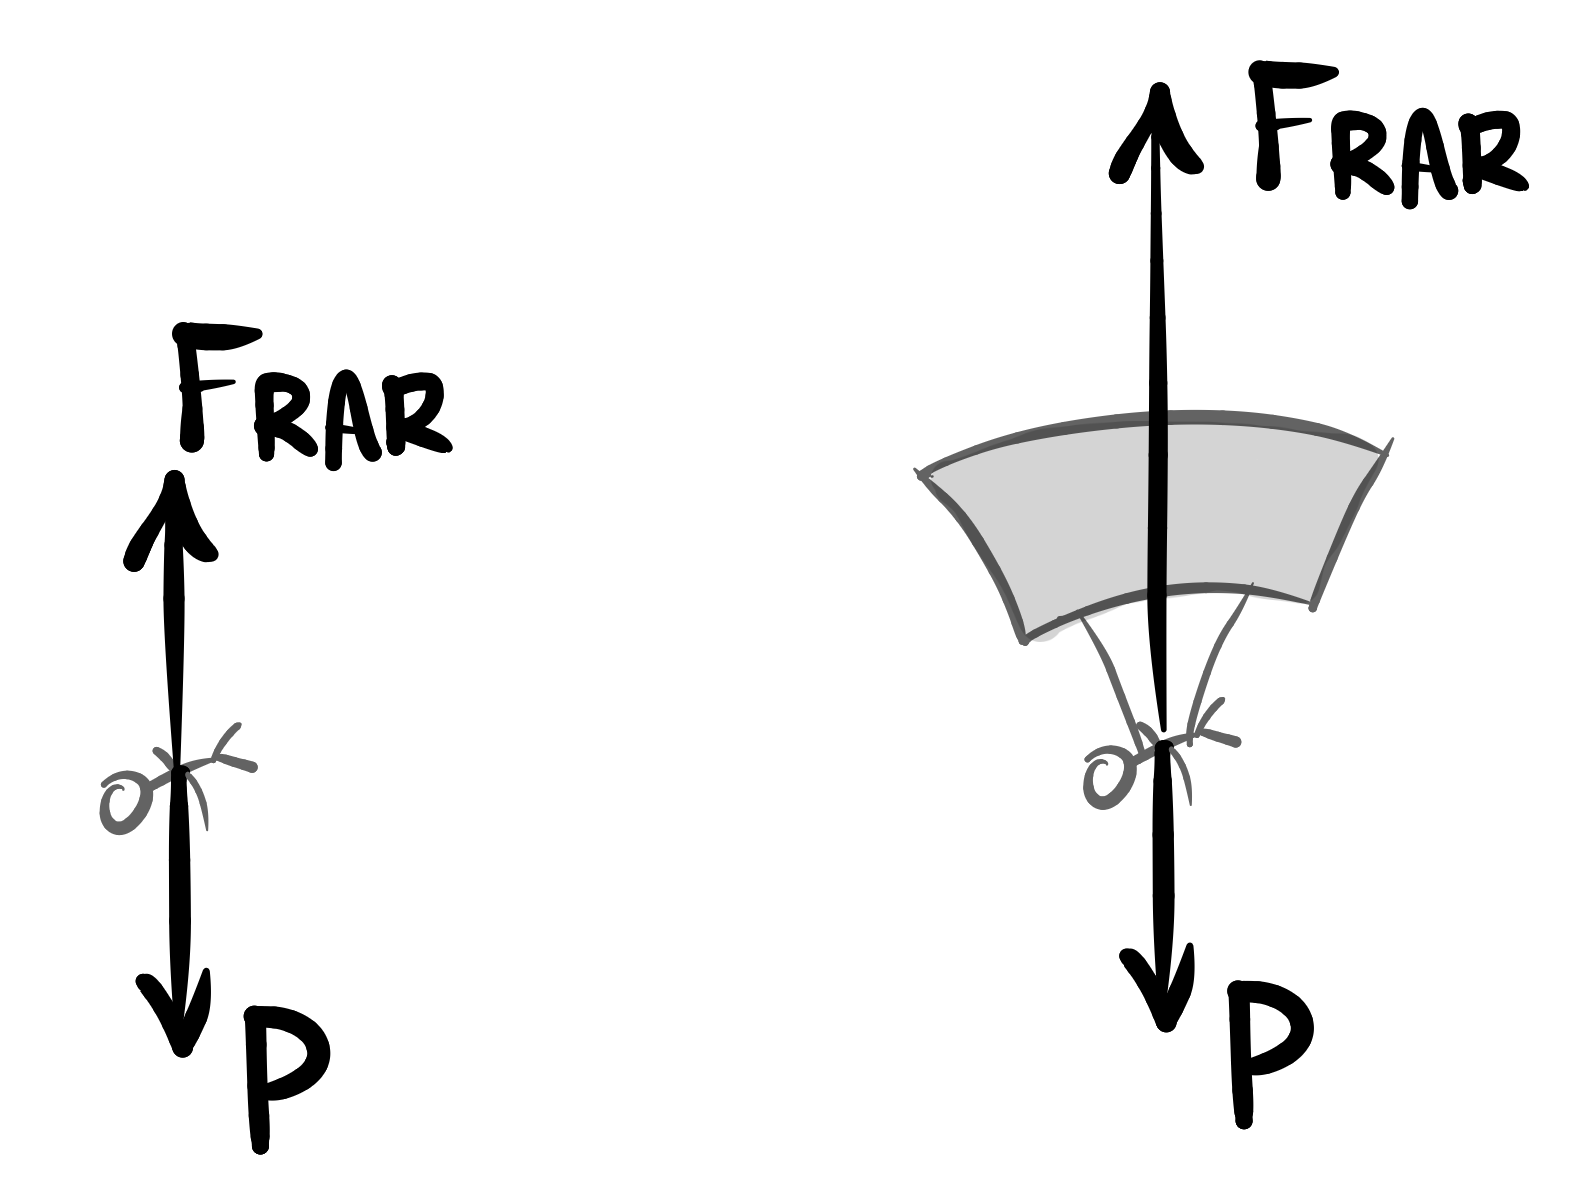
\includegraphics[width=0.35\linewidth]{imagensdinamicanewton/paraquedas.png}};
  \end{scope}
\end{tikzpicture}
\captionof{figure}{Abrir o paraquedas aumenta a área de colisão contra as partículas, aumentando a força de arrasto.}
\label{fig_mec_paraquedas}
} 
\vspace{0.3cm}

Assim, a partir de agora a força resultante se dirige para cima, uma vez que $F_{\text{RAR}}>P.$ Com isso, ela troca de sinal: se a força resultante inicialmente era positiva, para baixo, então uma força para cima deve ter sinal contrário, sendo, portanto, negativa. A partir deste instante o indivíduo começa a desacelerar. 

\medskip

Contudo, como sua velocidade diminui, a força de resistência do ar também irá diminuir, de modo que um processo análogo ao inicial irá acontecer: ela vai diminuindo até se igualar, novamente, ao peso. Neste caso, alcança-se uma nova velocidade terminal $v_T$, menor do que aquela primeira, de modo que o paraquedista pode pousar em segurança no solo.

\medskip

Desse modo, a segunda parte do gráfico de força, a partir de $T_A$, é análoga à primeira, trocando apenas de sinal: na primeira parte a força resultante começa para baixo e diminui até igualar ao peso. Na segunda, ela começa para cima e também diminui até igualar o peso. Como elas possuem sentidos contrários, os sinais também devem sê-lo, de modo que a resposta correta é a alternativa $(a).$

\end{exemplo}


\vspace{0.3cm}



\begin{exemplo}[Nível III]\label{exemplo_newton_frarex03}

Uma pedra de massa $m$ é solta em repouso do alto de um prédio e começa a cair sob a ação da força gravitacional e da força de resistência do ar, cujo módulo é dado por $|F_{\text{ar}}| = k\,|v|$, onde $v$ é a velocidade da pedra e $k$ é uma constante positiva. Sua velocidade, após um intervalo de tempo hipotético $t$, será:

\begin{enumerate}

\item [a)] $v = gt - k$

\item [b)] $v = \dfrac{mg}{k}\, e^{-\frac{k}{m}t}$

\item [c)] $v = \dfrac{mg}{k}\left(1 + e^{\frac{k}{m}t}\right)$

\item [d)] $v = \dfrac{mg}{k}\left(1 - e^{-\frac{k}{m}t}\right)$

\item [e)] $v = \dfrac{mg}{k}\left(1 + e^{-\frac{k}{m}t}\right)$

\end{enumerate}


\resolucao

Encontrar exatamente o formato da equação que descreve a velocidade é uma tarefa que exigiria o uso de ferramentas matemáticas mais sofisticadas do aquelas que se vê no Ensino Médio. Contudo, é possível respondermos a questão apenas com base no entendimento profundo do movimento que a pedra descreverá. \\

Note que este é, novamente, o mesmo problema que exploramos anteriormente, cujos gráficos estão representados na Figura \ref{fig_mec_frarqueda2}. Nós sabemos de duas informações importantes a respeito da velocidade, como o próprio gráfico de tal figura ilustra:

\begin{enumerate}
    \item [(i)] ela começa valendo zero em $t=0$, uma vez que é abandonada do repouso. Logo, qualquer que seja a expressão da velocidade em função do tempo $v(t),$ é preciso ter $v(0)=0.$

    \item [(ii)] a velocidade passa a ficar constante depois de um certo intervalo de tempo. Tal valor de velocidade -- a velocidade terminal $v_T$ -- é aquele para o qual a resistência do ar se iguala ao peso:

    $$ F_{\text{RAR}}=P \implies kv_{T} = mg \implies v_{T} = \dfrac{mg}{k}.$$

    Ou seja, sabemos que para um intervalo de tempo grande, isto é, se $t \to \infty,$ o valor da velocidade retornado pela função $v(t)$ deve ser igual a $\sfrac{mg}{k},$ ou seja:

    $$ t \to \infty \implies v(t) \to \dfrac{mg}{k}.$$
    
    \end{enumerate}

Assim, sabendo qual é o comportamento da velocidade nos extremos do intervalo de tempo -- em $t=0$ e em $t \to \infty$ -- será possível chegarmos à alternativa correta. Sobre o primeiro item, vemos que a alternativa $(a)$ fornece $v=-k$ em $t=0,$ o que está errado.

Para as demais alternativas o termo exponencial se tornará $1$ em $t=0$ -- haja vista que $a^0=1$ para todo $a \neq 0$ --, de modo que a alternativa $(b)$ diz que a velocidade da partícula no instante inicial é $\sfrac{mg}{k}$ e as alternativa $(c)$ e $(e)$ dizem que tal velocidade é $\sfrac{2mg}{k}.$ Portanto, a única alternativa condizente com o fato de que $v(0)=0$ -- isto é, a pedra é abandonada do repouso -- é a alternativa $(d),$ o que já nos possibilitaria marcá-la como a resposta correta. \\

Note, além disso, que quando $t \to \infty$, como tal expressão contém uma exponencial decrescente, o termo exponencial vai a zero quando $t$ cresce, de modo que a velocidade da partícula para valores grandes de $t$ se reduz para

$$ v(t \to \infty) = \dfrac{mg}{k} \left(1 - \cancelto{0}{e^{-\frac{k}{m}t}}\right) = \dfrac{mg}{k},$$

\noindent ou seja, a velocidade é igual à velocidade terminal $v_T,$ como esperado.

A única outra alternativa que também é condizente com este fato é alternativa $(e).$


\end{exemplo}


\vspace{0.3cm}



\begin{secnivel}[Força Resultante Centrípeta]{I}{Força Resultante Centrípeta}

  \eqLdois{dem}{eq_newton_forcacentripeta}{F_{\text{R}_\text{CPT}}=\dfrac{mv^2}{R}}

\end{secnivel}







\secgfe{De onde vem}

A Equação \eqref{eq_newton_forcacentripeta} não é, a bem da verdade, uma nova equação. Ela é simplesmente a Equação \eqref{cinvet_eq_aceleracaocentripeta} inserida na Equação \eqref{eq_dinamica1_segundaleinewton}, ou seja, trata-se da Segunda Lei de Newton aplicada na direção centrípeta, isto é:

$$ F_\text{R}=ma \implies F_{\text{R}_\text{CPT}}=ma_{_\text{CPT}} \implies F_{\text{R}_\text{CPT}}=m \dfrac{v^2}{R}. $$

Como, ao longo de um movimento circular, podemos usar a velocidade linear $v$ ou a velocidade angular $\omega$ para fazer a descrição cinemática, é possível reescrever a Equação \eqref{eq_newton_forcacentripeta} em termos da velocidade angular $\omega.$ Para isso, usamos a Equação \eqref{cinvet_eq_velangularelinear} e somos levados a

$$ F_{\text{R}_\text{CPT}}=m \dfrac{v^2}{R} \implies F_{\text{R}_\text{CPT}}=m \dfrac{(\omega R)^2}{R} \implies \boxed{F_{\text{R}_\text{CPT}}=m \omega^2R,}$$

\noindent que é exatamente a Equação \eqref{eq_newton_forcacentripeta}, porém escrita em termos da velocidade angular $\omega$ no lugar da velocidade linear $v$.


\secgfe{Onde é usada}

Como já vimos no estudo da Equação \eqref{cinvet_eq_aceleracaocentripeta}, na análise da dinâmica de qualquer movimento que faça algum tipo de curva, sempre existirá uma aceleração -- responsável por variar a direção do vetor velocidade e, portanto, responsável por permitir com que o corpo faça curva -- que aponta para o centro de curvatura do movimento, chamada de aceleração centrípeta. 

Contudo, qualquer aceleração é sempre um efeito gerado por uma resultante de forças, como indica a Equação \eqref{eq_dinamica1_segundaleinewton}. Logo, para haver uma aceleração que aponta para o centro de curvatura -- aceleração centrípeta -- é preciso haver uma resultante de forças que aponta para o centro de curvatura: é o que chamamos de força resultante centrípeta, $F_{\text{R}_\text{CPT}}$. 

Sendo assim, no estudo da dinâmica de absolutamente qualquer movimento curvilíneo, a Equação \eqref{eq_newton_forcacentripeta} será útil: ela computa qual deve ser o valor da força resultante que aponta para o centro, capaz de gerar a aceleração centrípeta necessária para que o corpo execute aquela curva.

Como mostra a primeira imagem da Figura \ref{fig_mec_newtonfcpt01}, se um corpo estiver se movendo com uma aceleração $\vec{a}$ ao longo do plano inclinado, a Equação \eqref{eq_dinamica1_segundaleinewton} nos diz que deve existir uma resultante de forças $\vec F_{\text{R}}$ que aponta na mesma direção e sentido de tal aceleração, sendo responsável por gerá-la.


\vspace{0.3cm}
{
\centering
\begin{tikzpicture}
  \begin{scope}[blend mode=multiply]
    \node {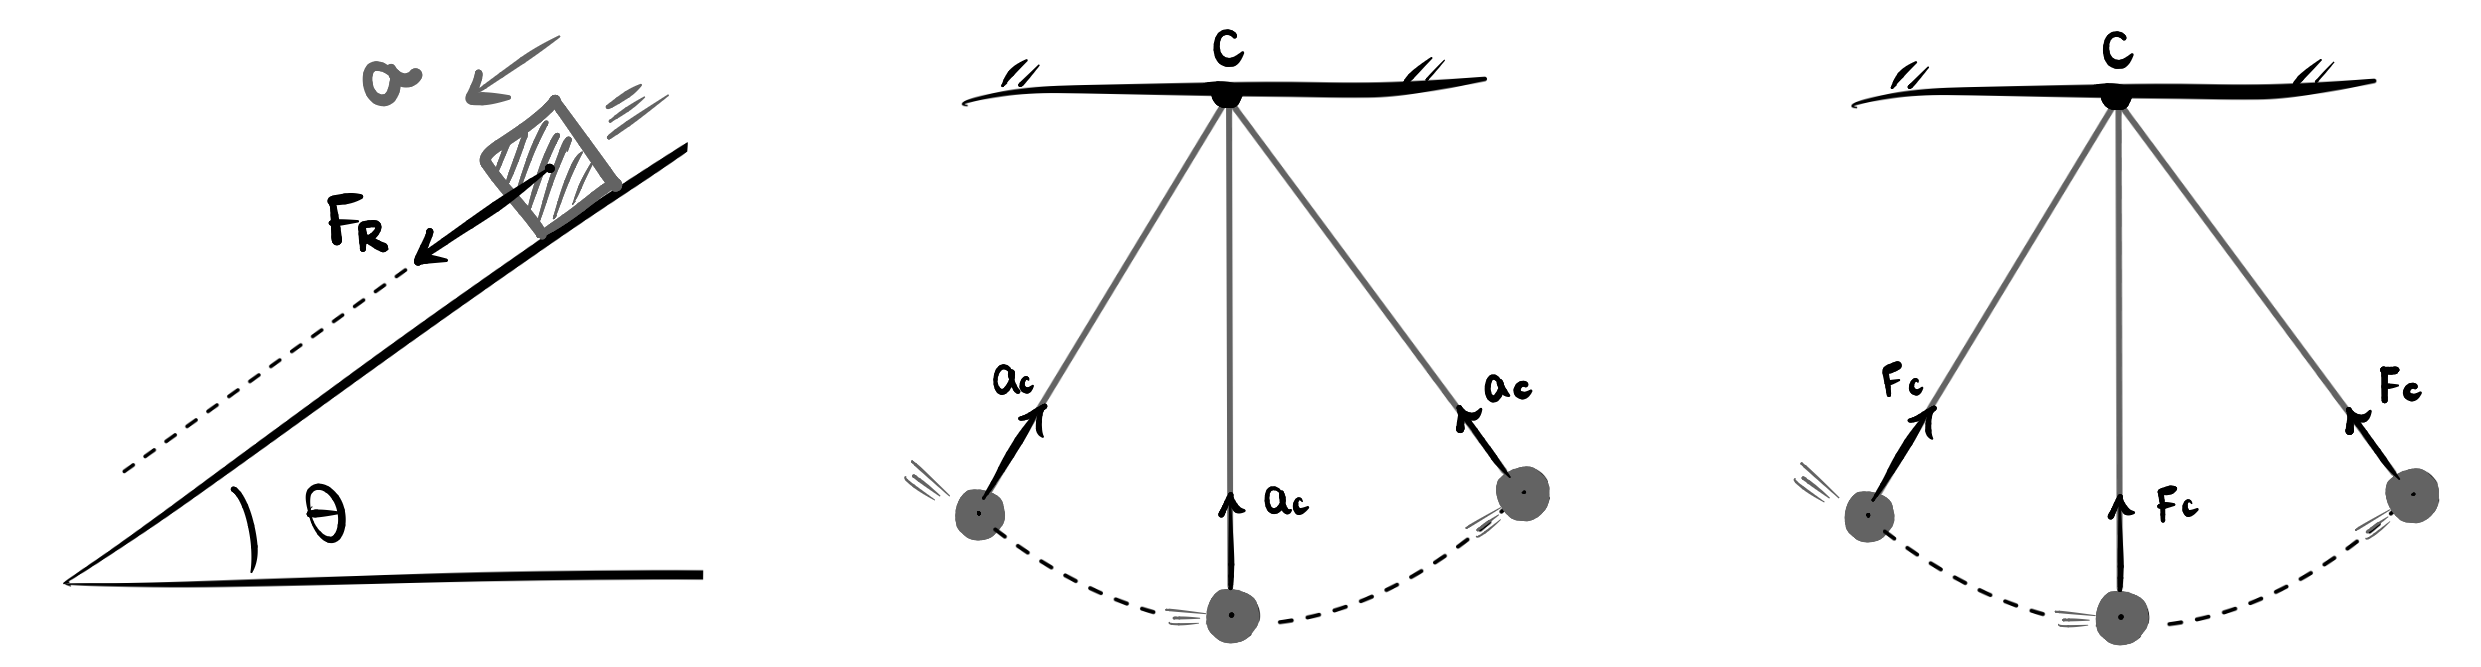
\includegraphics[width=0.8\linewidth]{imagensdinamicanewton/newtonforcacpt1.png}};
  \end{scope}
\end{tikzpicture}
\captionof{figure}{Qualquer aceleração -- centrípeta ou tangencial -- é gerada por uma força resultante, como diz a Segunda Lei de Newton.}
\label{fig_mec_newtonfcpt01}
} 
\vspace{0.3cm}

O mesmo vale para a situação da segunda imagem, que mostra um corpo descrevendo um movimento ao longo de um arco de circunferência. Por ser um movimento curvo, deve sempre haver uma aceleração centrípeta $\vec a_\text{c}$ apontando para o centro de curvatura $C$ do movimento. Logo, a Equação \eqref{eq_dinamica1_segundaleinewton} nos diz que deve existir uma resultante de forças $\vec F_{\text{R}_{\text{C}}}$ que aponta na mesma direção e sentido de tal aceleração -- ou seja, para o centro -- sendo responsável por gerá-la, como mostra a última imagem da figura.

% Assim, em todo movimento que faça curva haverá uma resultante de forças apontando para o centro, responsável por gerar a aceleração centrípeta. A Equação \eqref{eq_newton_forcacentripeta} calcula justamente quanto deve valer tal força resultante na direção do centro.



\secgfe{Erros comuns}

O erro mais comum é o estudante pensar que a Equação \eqref{eq_newton_forcacentripeta} define ou cria um novo tipo de força, a chamada \textit{força centrípeta.} Isso seria o mesmo que dizer que a Equação \eqref{eq_dinamica1_segundaleinewton} define (ou cria) um novo tipo de força: a força resultante $F_{\text{R}}$, o que não ocorre.


Considere, novamente, as duas situações da Figura \ref{fig_mec_newtonfcpt01}. Na primeira delas temos um corpo acelerando plano abaixo. Quais seriam as forças que atuam em tal corpo? A primeira imagem da Figura \ref{fig_mec_newtonfcpt02} mostra tal diagrama de forças: existe a força peso, trocada entre a caixa e a terra, e as forças de atrito e normal, trocadas entre a caixa e o plano.

\vspace{0.3cm}
{
\centering
\begin{tikzpicture}
  \begin{scope}[blend mode=multiply]
    \node {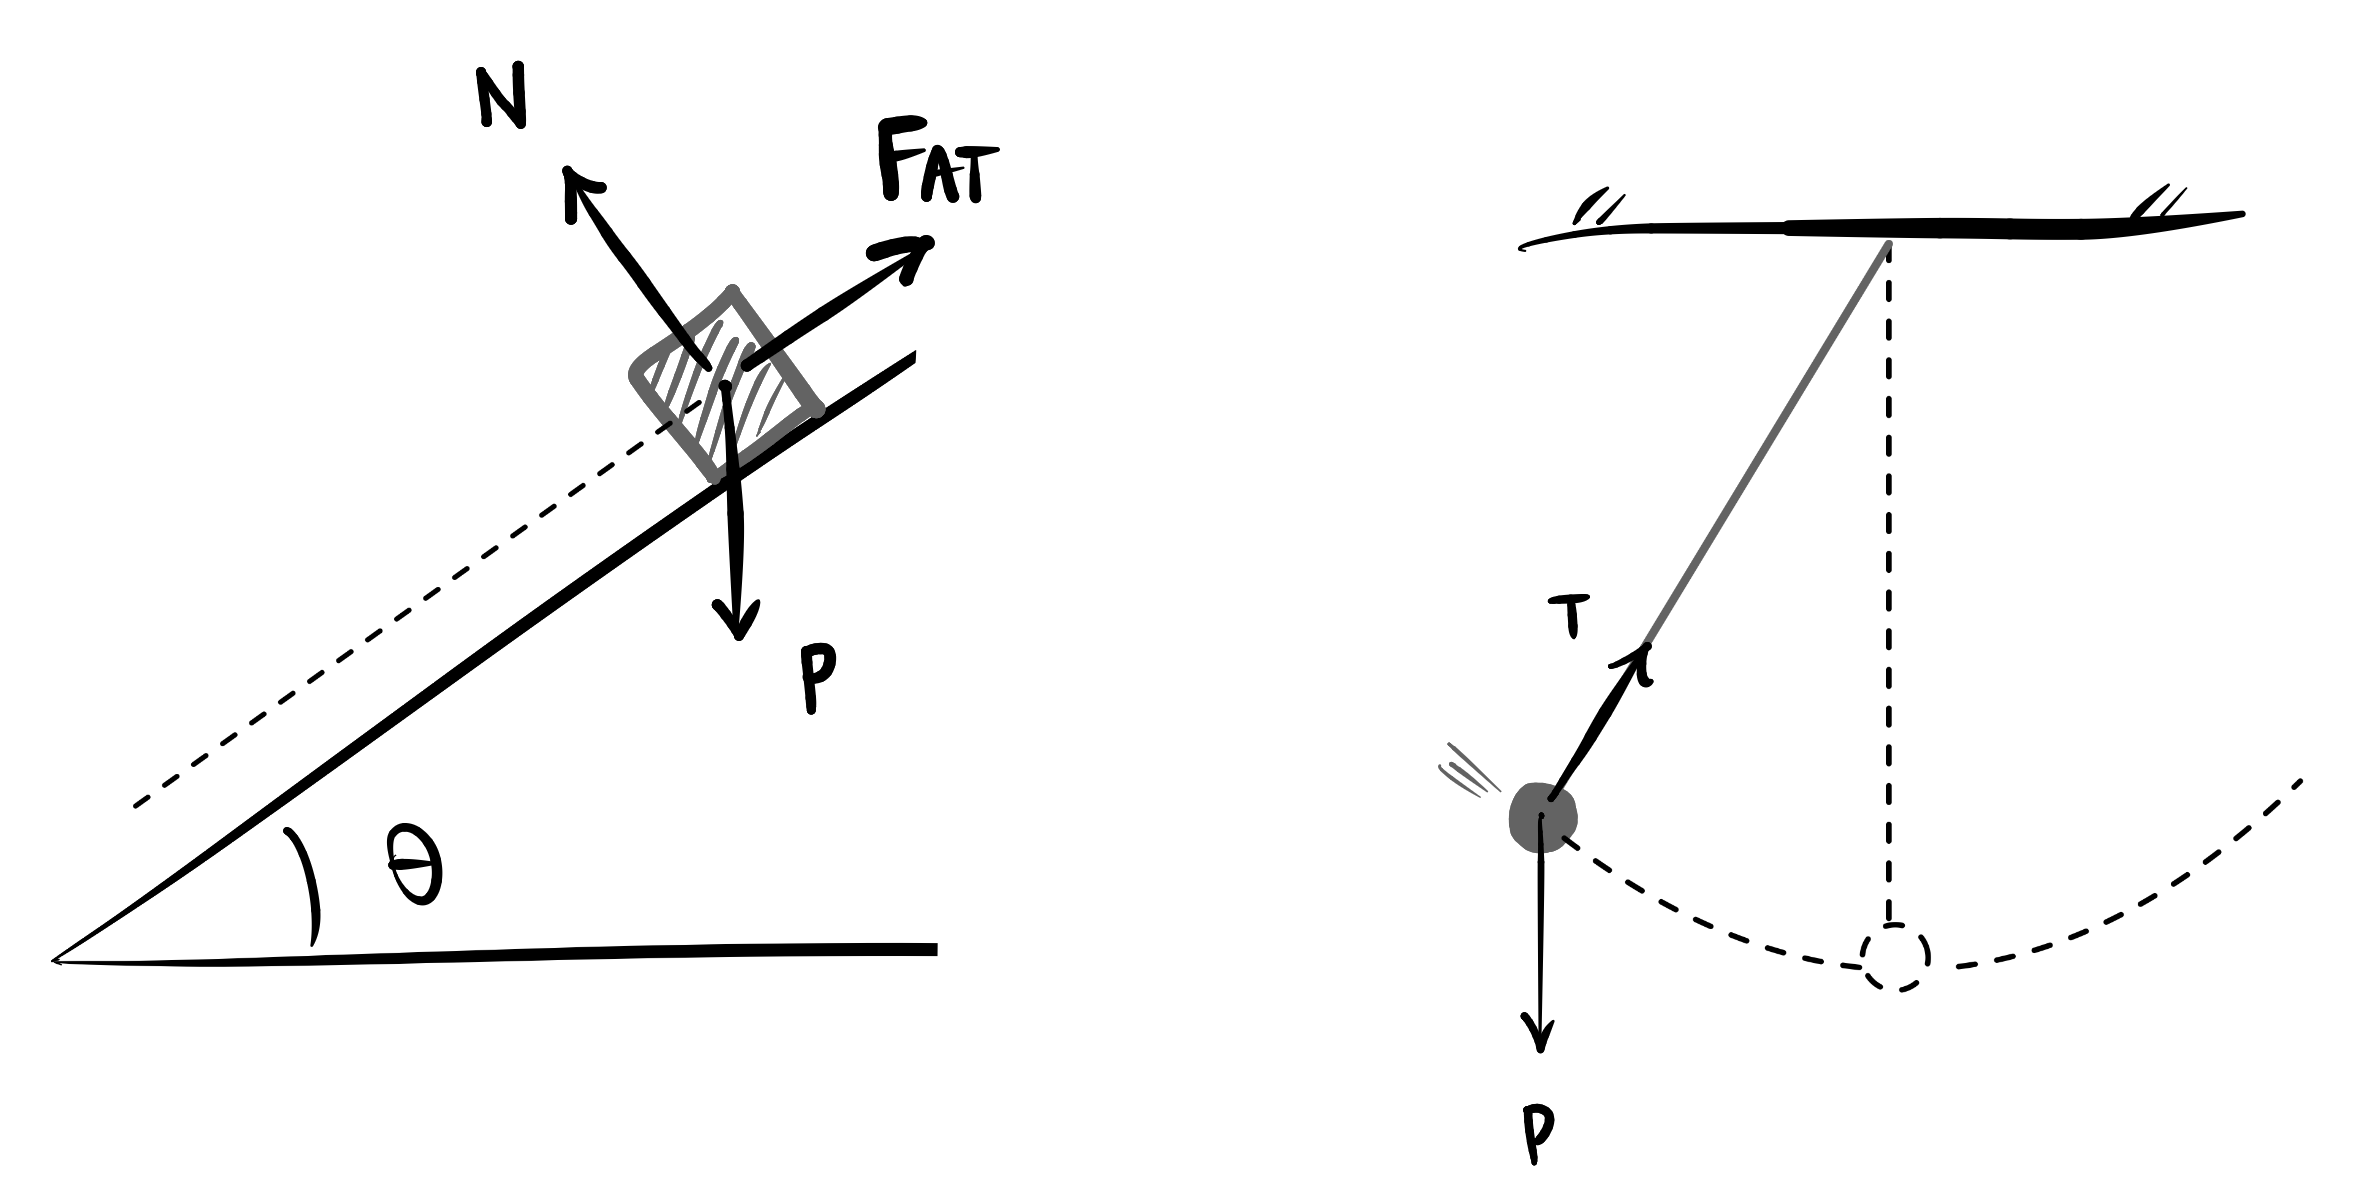
\includegraphics[width=0.6\linewidth]{imagensdinamicanewton/newtonforcacpt2.png}};
  \end{scope}
\end{tikzpicture}
\captionof{figure}{Forças criam acelerações. Assim, o cálculo de $F_{\text{R}} =ma$ não cria uma nova força $F_{\text{R}},$ apenas calcula o valor da resultante das forças necessária para gerar a aceleração $a$ no corpo.}
\label{fig_mec_newtonfcpt02}
} 
\vspace{0.3cm}

Perceba que não existe uma quarta força $F_{\text{R}},$ chamada força resultante. Esta é, na verdade, a resultante das três forças que atuam na caixa. Forças sempre exigem agentes que as executem: a força peso é exercida pelo campo gravitacional da Terra, a força normal é uma força de reação à compressão exercida pelo plano sob a caixa e a força de atrito é uma força de resistência à tendência de movimento, exercida também pelo plano sob a caixa.

Se quiséssemos desenhar uma quarta força, chamada força resultante, eu perguntaria ao leitor: \textit{quem seria o agente que exerce tal força?} Perceba que não haveria nenhum, o que mostra que não existe um novo ente chamado ``\textit{força resultante}.'' Ela é apenas a resultante vetorial das forças que conhecemos e, no caso do plano inclinado, tal resultante deve apontar na direção do plano, sendo responsável por gerar a aceleração do bloco nessa direção.



O mesmo ocorre para a situação da segunda imagem da Figura \ref{fig_mec_newtonfcpt01}: não existe um agente responsável por fazer uma força centrípeta que aponta na direção do centro. O que existem são as forças que conhecemos: força de tração, força normal, força elástica, força peso, força de atrito, etc. E é a resultante dessas forças que devem ter uma componente na direção do centro, responsável por gerar a aceleração centrípeta. 

A segunda imagem da Figura \ref{fig_mec_newtonfcpt02} mostra essa situação: as forças que atuam na bolinha em movimento circular são a tração -- exercida pelo fio -- e a força peso -- exercida pela Terra --, e é a resultante dessas duas que deve dar uma componente que aponta para o centro, sendo, portanto, responsável por gerar a aceleração centrípeta.

Note, assim, que a Equação \eqref{eq_newton_forcacentripeta} não define nem cria um novo tipo de força que aponta para o centro -- a tal \textit{força centrípeta}. Esta última sequer existe: o que existe são as forças que já conhecemos, e elas devem se somar e se cancelar de modo a sobrar uma componente que aponte para o centro -- a resultante das forças na direção centrípeta (ou força resultante centrípeta).




\secgfe{Observações}

Até aqui ficou claro para o leitor que, se existe uma aceleração, deve haver uma resultante de forças apontando para a mesma direção e sentido de tal aceleração, responsável por gerá-la. A imagem da Figura \ref{fig_mec_fcptpendulosimplesanalise1} evidencia este fato: em um movimento curvilíneo\footnote{O movimento não precisa ser circular: qualquer que seja o tipo de curva será exigido aceleração centrípeta para realizar tal movimento.}, sempre haverá uma aceleração $a_c$ apontando para o centro $O$, de modo que sempre teremos uma resultante de forças $F_{\text{R}_{\text{C}}}$ apontando para o centro, responsável por gerar tal aceleração.

Contudo, apesar de isso estar correto, a força resultante total que atua no corpo não aponta necessariamente para o centro em todos os pontos, como a Figura \ref{fig_mec_fcptpendulosimplesanalise1} leva a crer.

\vspace{0.3cm}
{
\centering
\begin{tikzpicture}
  \begin{scope}[blend mode=multiply]
    \node {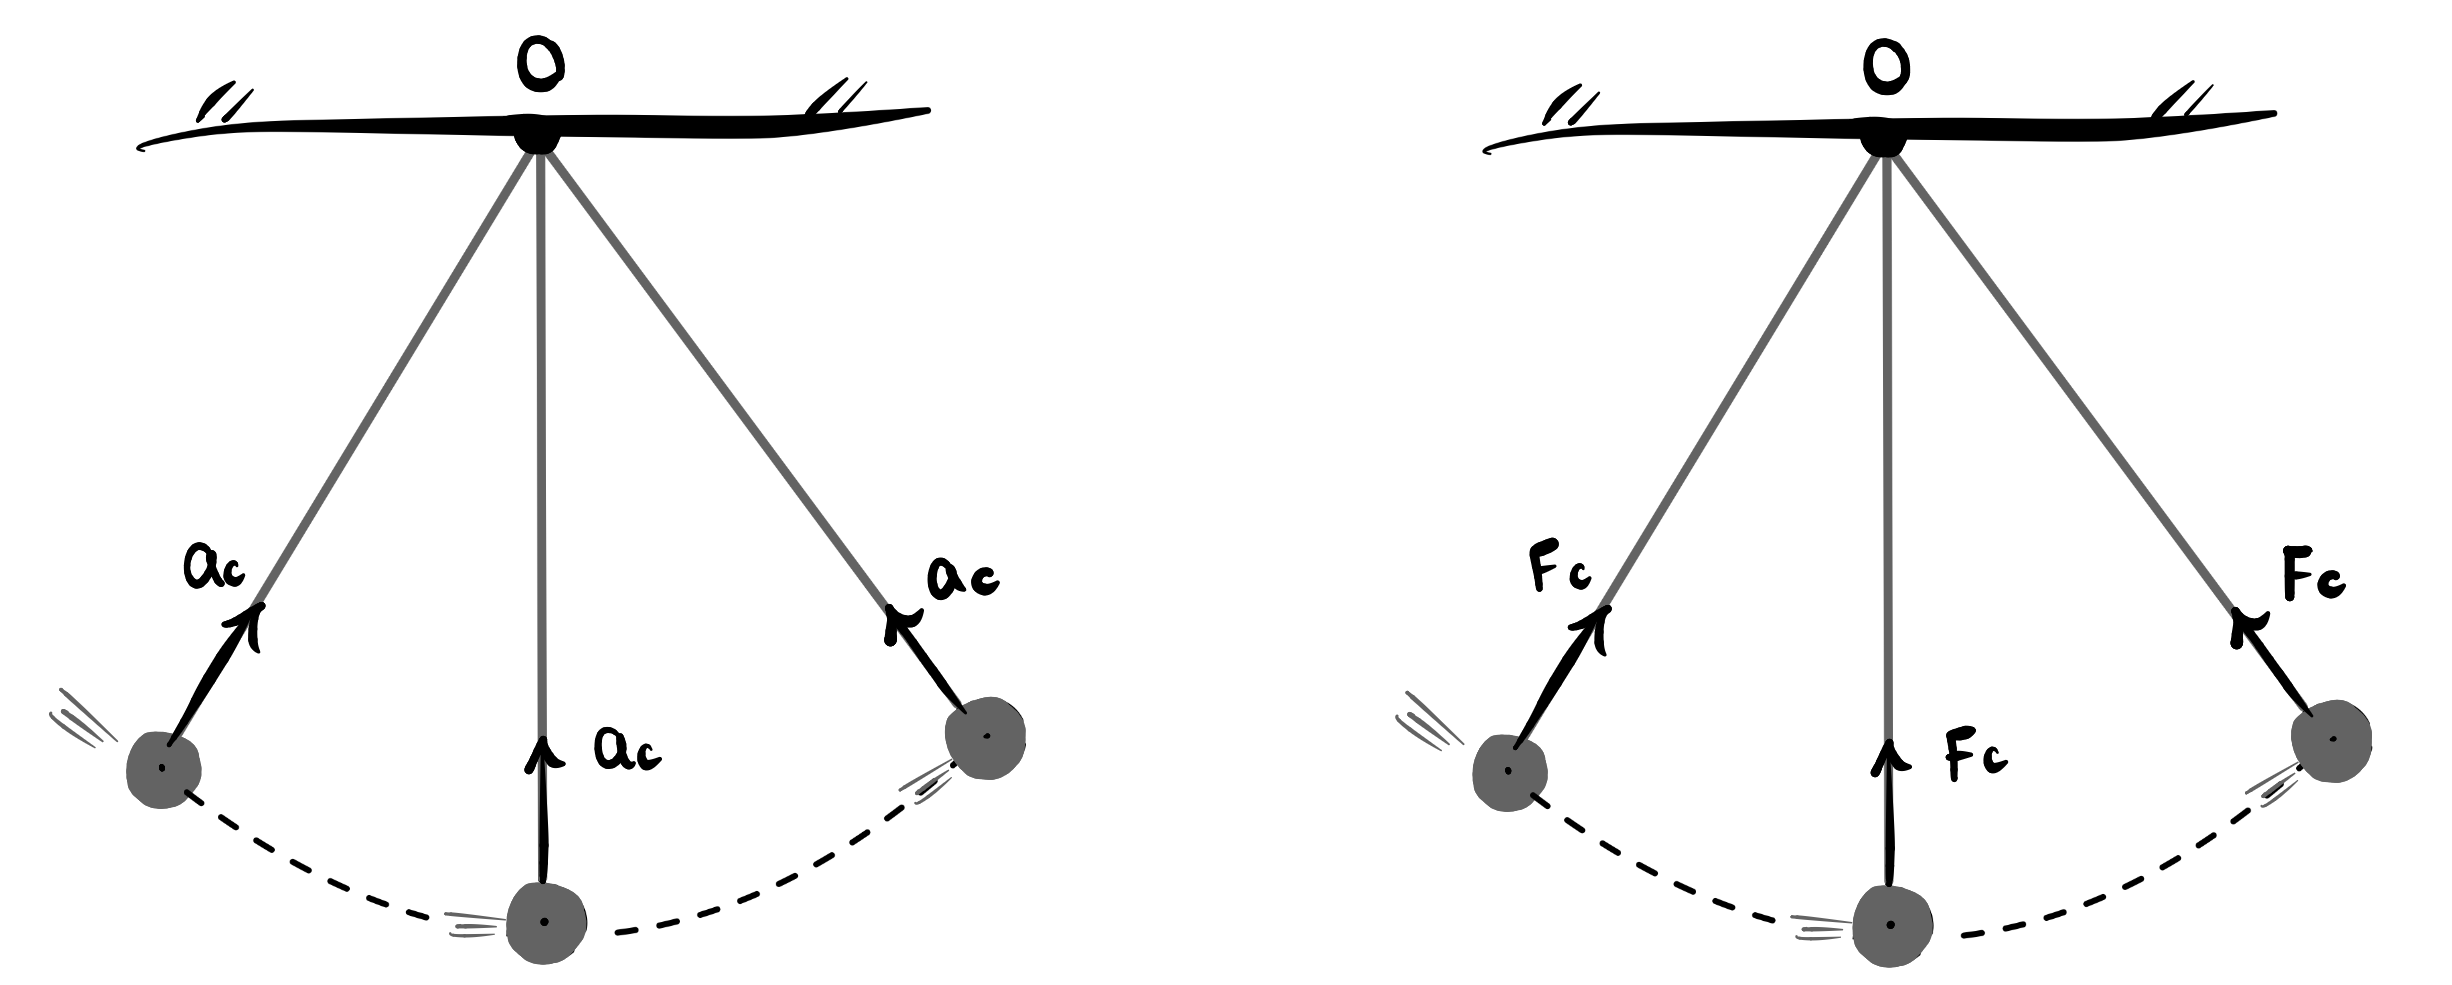
\includegraphics[width=0.6\linewidth]{imagensdinamicanewton/fcptpendulosimplesanalise1.png}};
  \end{scope}
\end{tikzpicture}
\captionof{figure}{A aceleração exige uma força que a cause.}
\label{fig_mec_fcptpendulosimplesanalise1}
} 
\vspace{0.3cm}


Para compreendermos isso é importante que o leitor tenha estudado e compreendido todos os detalhes do desenvolvimento e significado das Equações \eqref{eq_dinamica1_segundaleinewton} e \eqref{cinvet_eq_aceleracaocentripeta}. A análise da dinâmica das forças no pêndulo em qualquer instante é feita na Figura \ref{fig_mec_fcptpendulosimplesanalise2}. Para um ponto qualquer do movimento do pêndulo, sempre teremos apenas duas forças atuando: o seu peso, dirigido verticalmente para baixo, e a tração no fio, que atua ao longo da direção do fio. 

\vspace{0.3cm}
{
\centering
\begin{tikzpicture}
  \begin{scope}[blend mode=multiply]
    \node {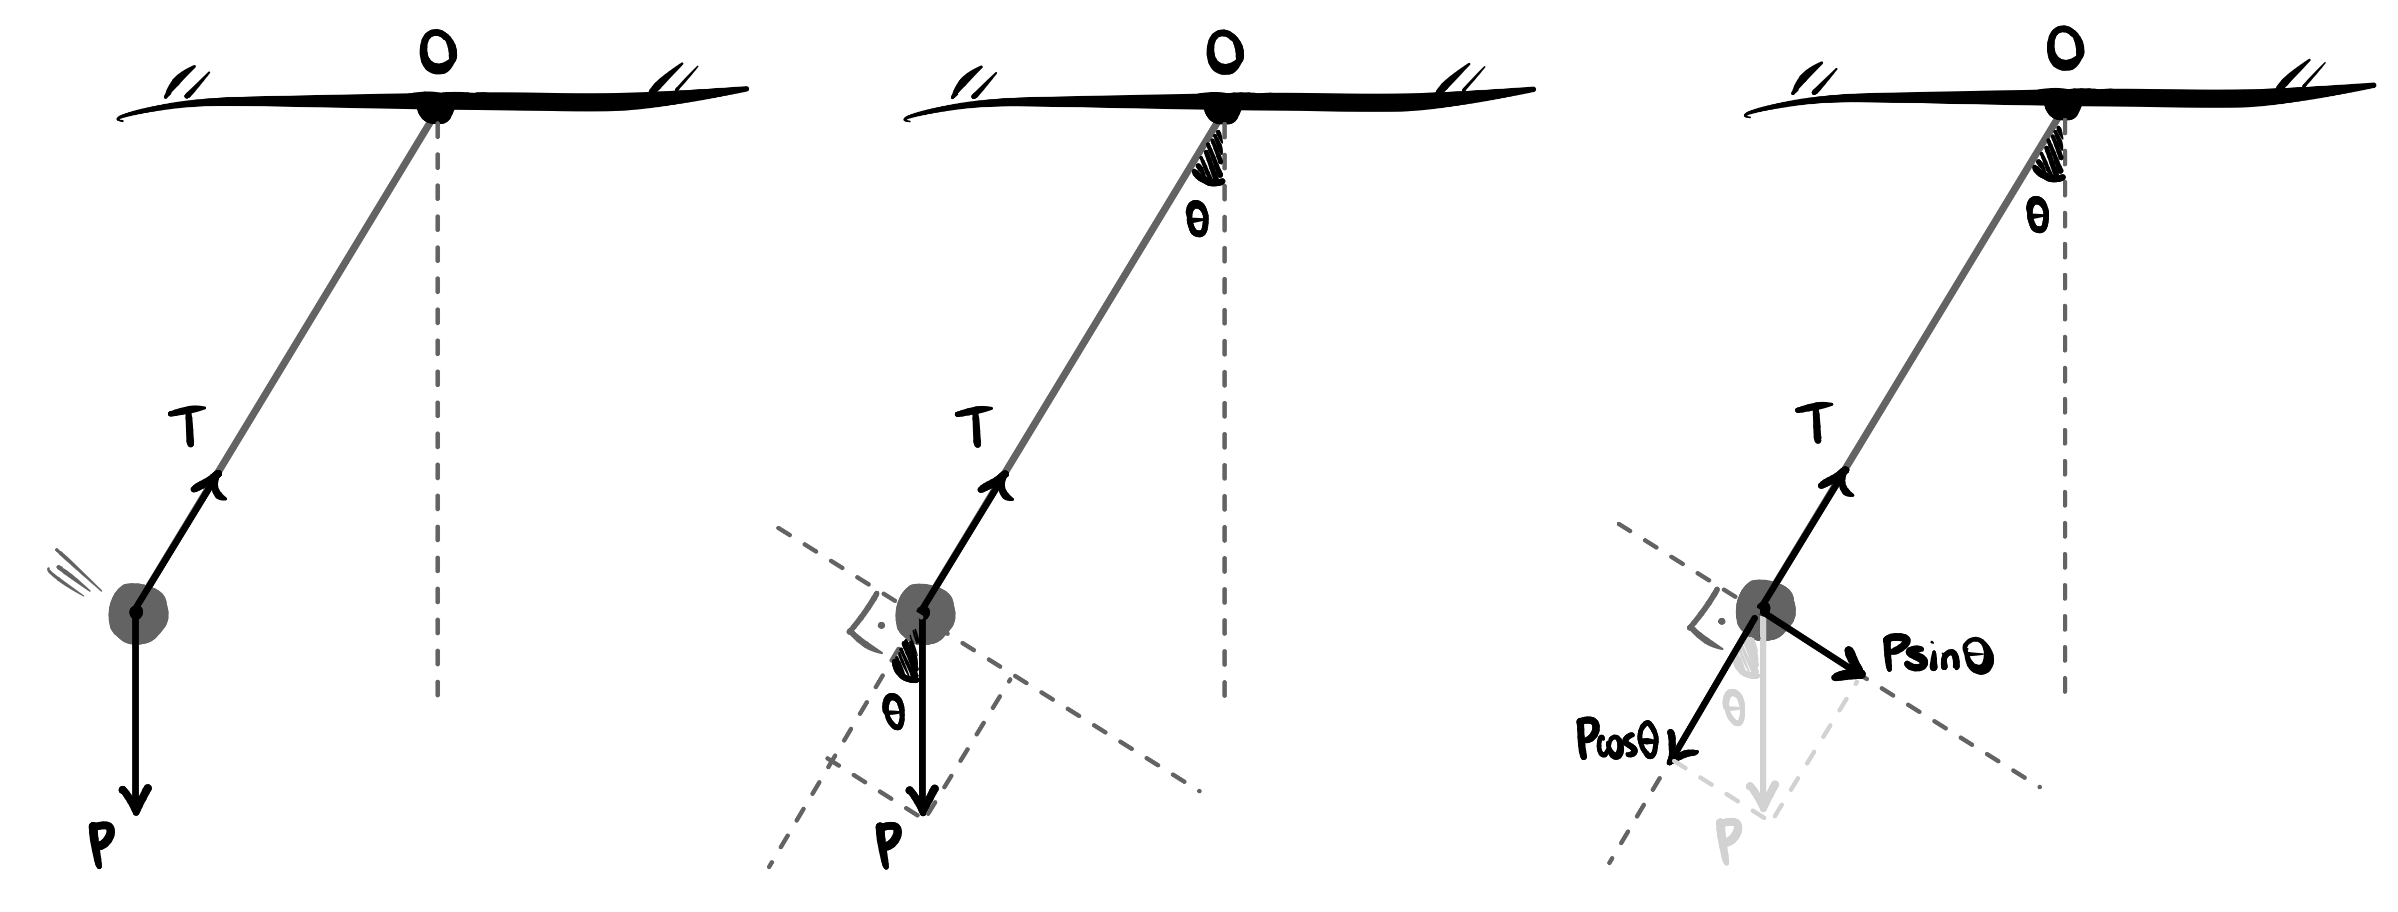
\includegraphics[width=0.8\linewidth]{imagensdinamicanewton/fcptpendulosimplesanalise2.png}};
  \end{scope}
\end{tikzpicture}
\captionof{figure}{As forças sempre serão decompostas no eixo centrípeto e tangencial.}
\label{fig_mec_fcptpendulosimplesanalise2}
} 
\vspace{0.3cm}

Como já sabemos, os eixos de decomposição das forças sempre serão aquele paralelo à velocidade (eixo tangencial) e o perpendicular a ele (eixo centrípeto, neste caso). Assim, estando a tração ao longo de um desses eixos (eixo centrípeto) é necessário decompor apenas a força peso, que possui componente na direção tangencial e centrípeta. Avaliemos separadamente cada uma dessas direções.

\begin{enumerate}
    \item [(i)] O peso possui uma componente tangencial $P_{\text{T}}=P \sin \theta$, que é responsável por gerar a aceleração tangencial $a_{\text{T}}$:

    $$F_{\text{R}_{\text{T}}} = m a_{\text{T}} \implies mg \sin \theta =  m a_{\text{T}} \implies  \boxed{ a_{\text{T}} = g \sin \theta,} $$
    
    
    \noindent ou seja, a aceleração tangencial é exatamente como aquela em um plano inclinado, que faz o pêndulo acelerar plano abaixo na descida ou desacelerar na subida.
    
    A Figura \ref{fig_mec_fcptpendulotangencial} mostra essa análise: na descida, de $A$ até $C$, é como se o pêndulo fosse descendo ao longo de planos inclinados de inclinações cada vez menores, até atingir a inclinação zero no ponto mais baixo da trajetória (ponto $C$), no qual a aceleração tangencial seria zero -- a bolinha seguiria em MRU na horizontal se a tração, neste ponto, não fosse maior que o peso, o que a obriga a subir. 

\vspace{0.3cm}
{
\centering
\begin{tikzpicture}
  \begin{scope}[blend mode=multiply]
    \node {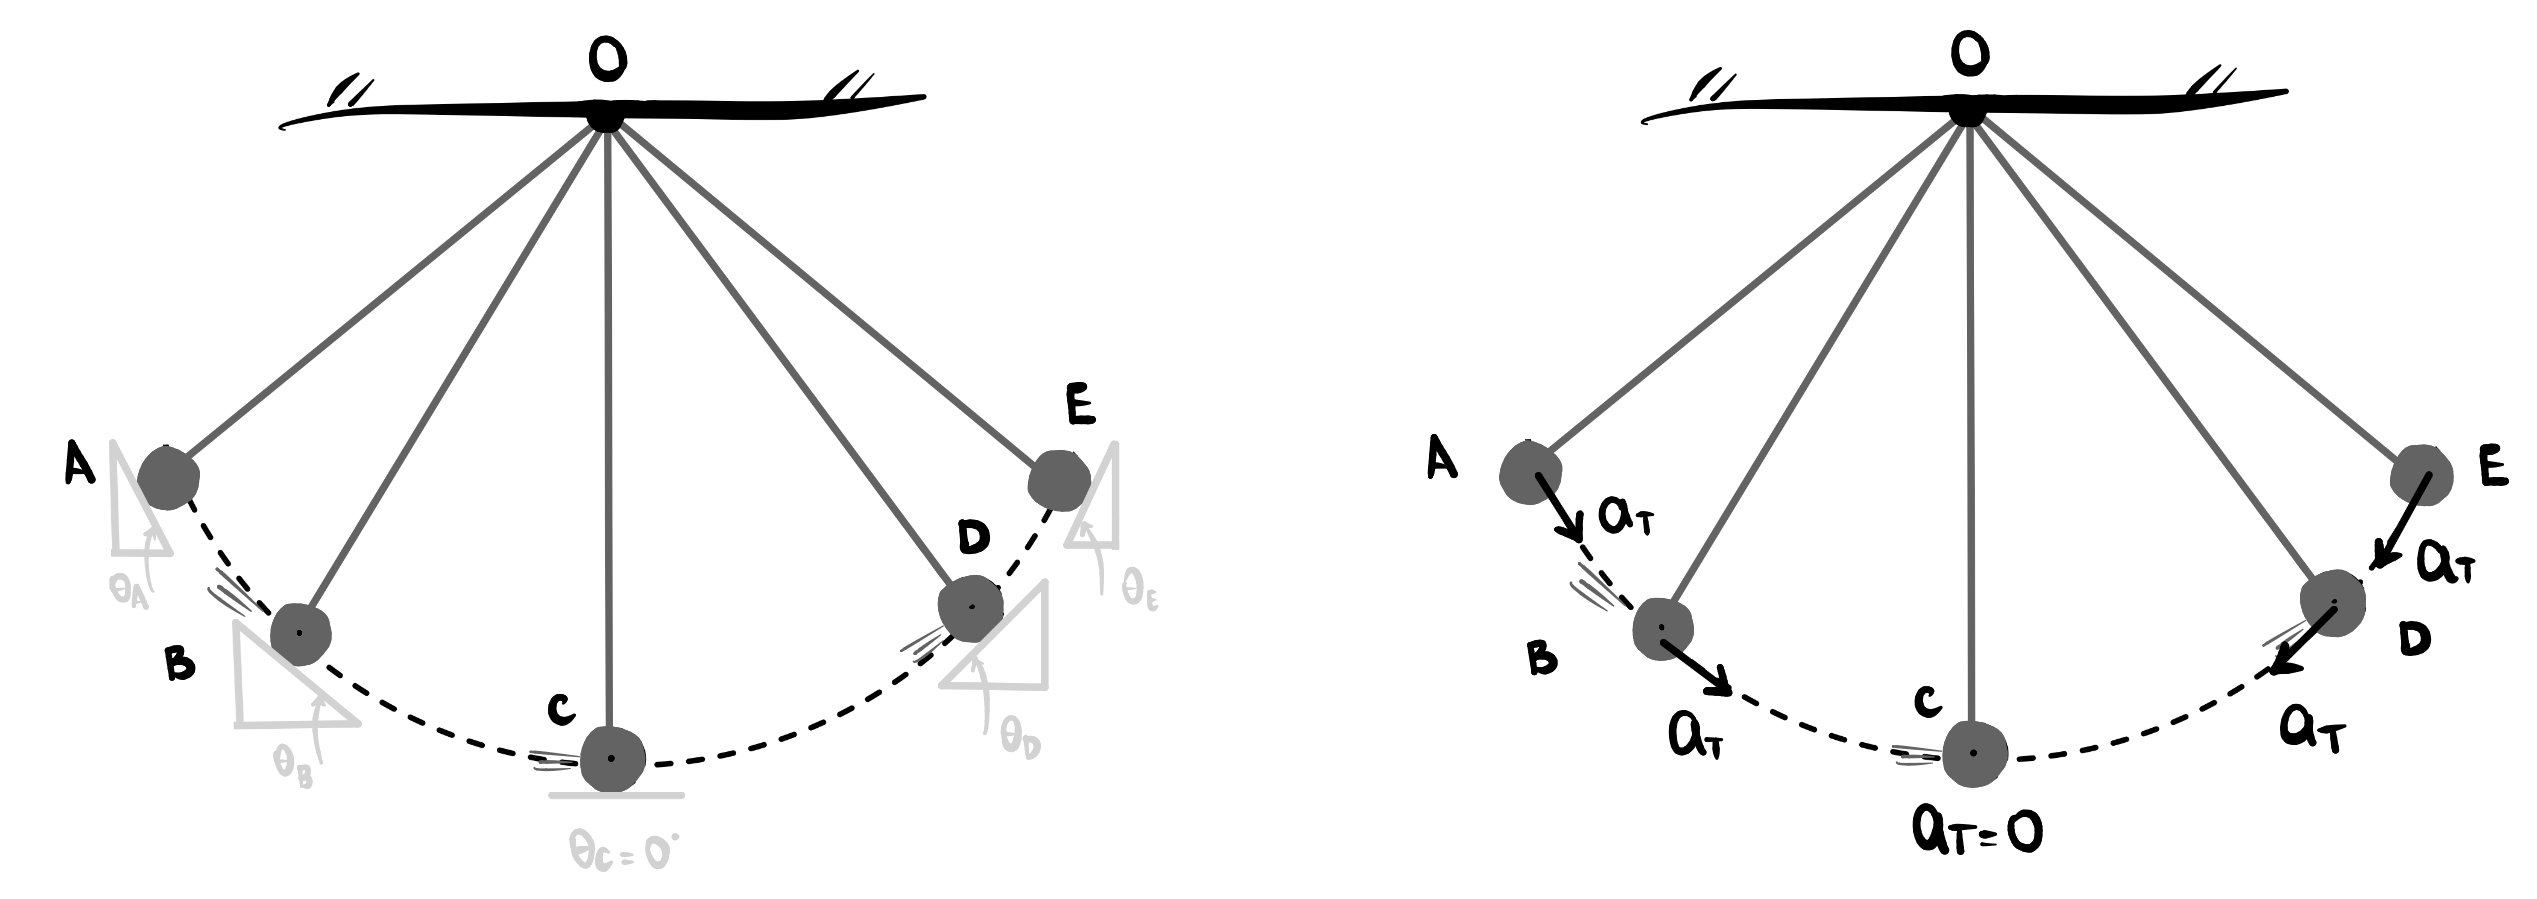
\includegraphics[width=0.9\linewidth]{imagensdinamicanewton/fcptpendulotangencial.png}};
  \end{scope}
\end{tikzpicture}
\captionof{figure}{A análise das forças na direção tangencial.}
\label{fig_mec_fcptpendulotangencial}
} 
\vspace{0.3cm}
    
    Assim, na subida, de $C$ até $E,$ é como se a bolinha subisse ao longo de planos inclinados de inclinações cada vez maiores, desacelerando até parar momentaneamente no ponto $E.$ Neste ponto, é como se ela fosse abandonada de um plano inclinado de inclinação $\theta_E,$ o que a faria acelerar plano abaixo, descrevendo o mesmo movimento da ida, porém agora descendo e acelerando de $E$ até $C$ e depois subindo em movimento desacelerado de $C$ até $A,$ ponto em que a velocidade zera e a bolinha inverteria novamente o sentido do seu movimento.





Essa é a análise da resultante das forças na direção tangencial -- e, portanto, da componente tangencial da aceleração -- da bolinha ao longo de seu movimento.

    \item [(ii)] O peso possui também uma componente centrípeta $P_{\text{C}}=P \cos \theta$, que aponta para fora do centro da curva. É a resultante das forças nessa direção que gera a aceleração centrípeta:

    \begin{align}
         F_{\text{R}_\text{CPT}} &= F_{\text{DENTRO}} - F_{\text{FORA}}  \nonumber \\
                                 &= T - P \cos \theta, \nonumber
    \end{align}
 \noindent e, pela Equação \eqref{eq_newton_forcacentripeta}, teremos

 $$ \boxed{F_{\text{R}_\text{CPT}}=T - P \cos \theta = \dfrac{mv^2}{R}.}$$

 A resultante na direção centrípeta sempre seguirá essa premissa: será a resultante de todas as forças que apontam para dentro, ou seja, para o centro da curva ($F_{\text{DENTRO}}$) subtraída da resultante de todas as forças que apontam para fora do centro da curva ($F_{\text{FORA}}$). 
 
 
 \vspace{0.3cm}
 {
\centering
\begin{tikzpicture}
  \begin{scope}[blend mode=multiply]
    \node {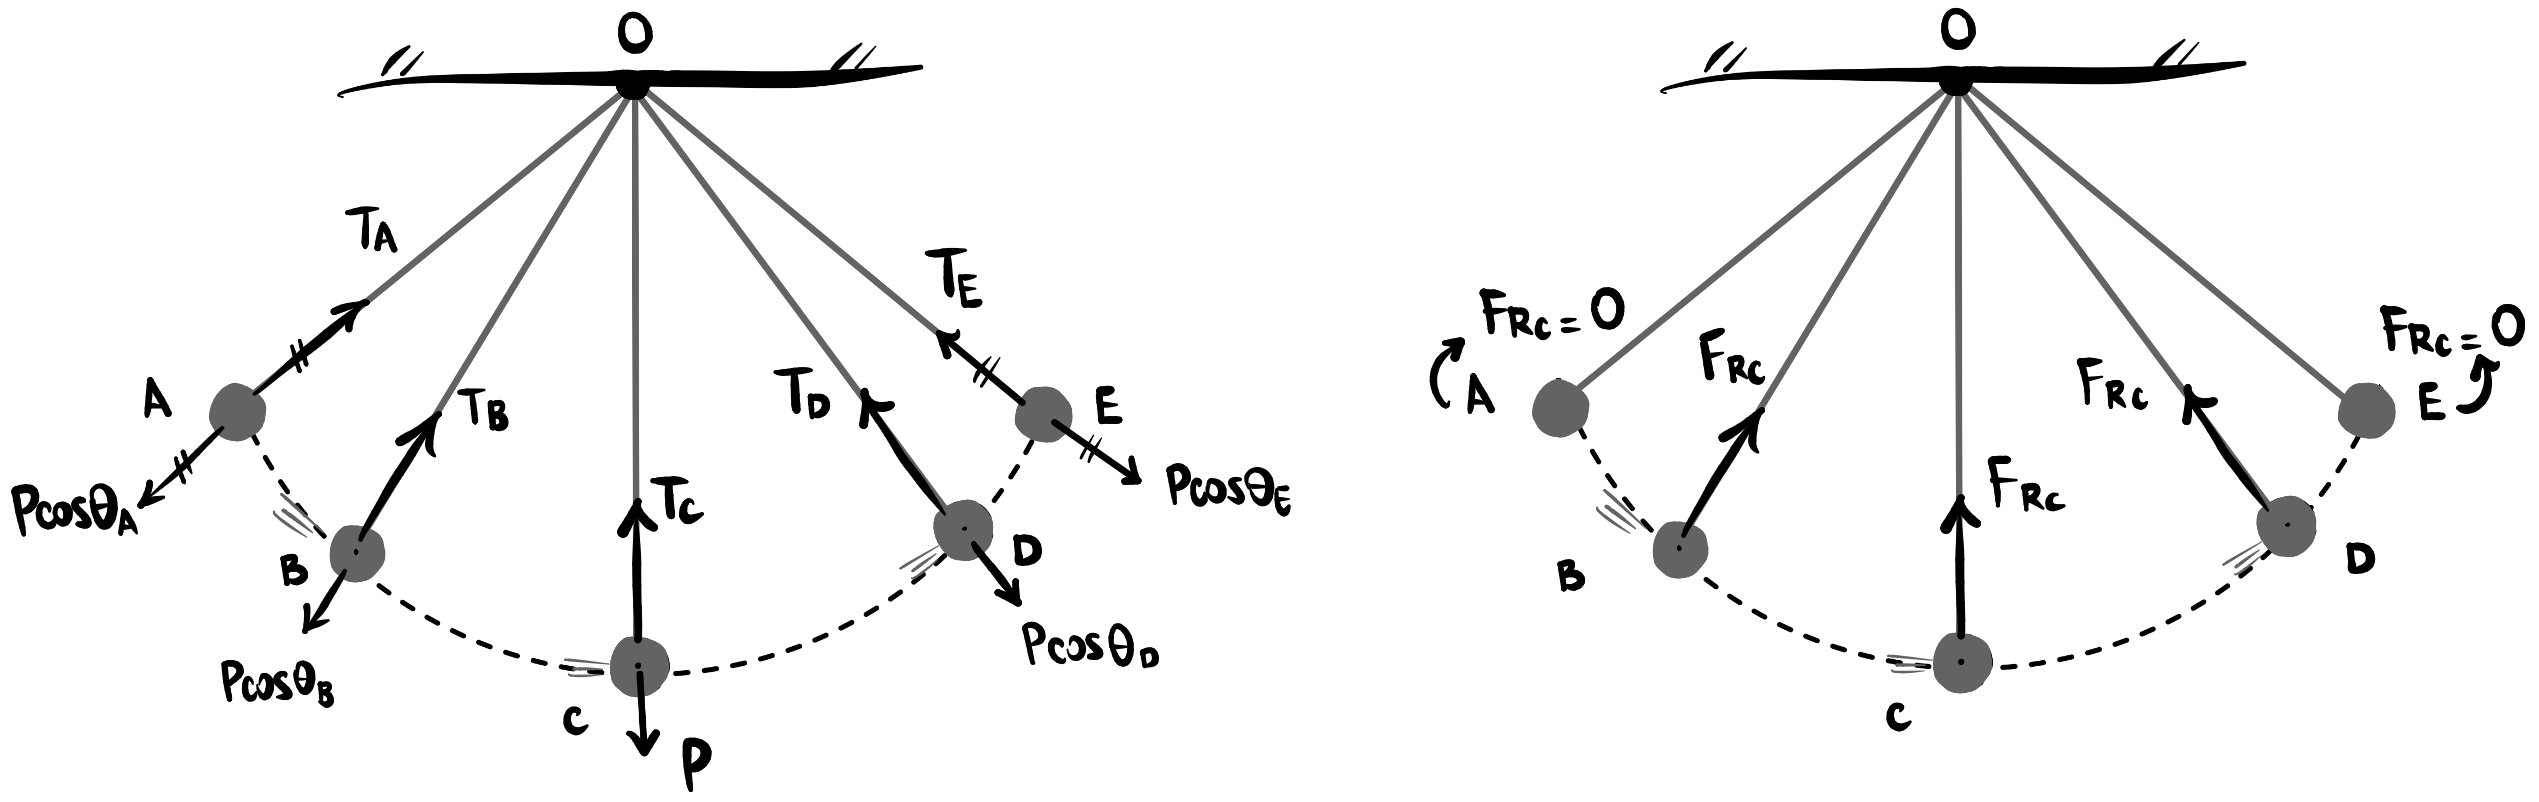
\includegraphics[width=0.9\linewidth]{imagensdinamicanewton/fcptpendulocentripeto.png}};
  \end{scope}
\end{tikzpicture}
\captionof{figure}{A análise das forças na direção centrípeta.}
\label{fig_mec_fcptpendulocentripeto}
} 
\vspace{0.3cm}
 
 
 A Figura \ref{fig_mec_fcptpendulocentripeto} mostra a análise da resultante na direção centrípeta -- dada pela equação em destaque acima -- para os diferentes pontos do movimento do pêndulo:

 \begin{enumerate}
     \item [A)] Neste ponto extremo a velocidade da partícula é zero -- é o ponto de inversão do sentido de seu movimento -- de modo que a resultante centrípeta é

     $$ F_{\text{R}_\text{CPT}}= T_{\text{A}} - P \cos \theta_{\text{A}} = \dfrac{m \cancelto{0}{v^2}}{R} =0 \implies \boxed{ T_{\text{A}} = P \cos \theta_{\text{A,}}}$$
     
     \noindent ou seja, as forças se anulam na direção centrípeta: neste ponto a aceleração centrípeta (e, portanto, a força resultante na direção centrípeta) são nulas.

     \item[B)] Neste ponto, como temos $v \neq 0,$ a aceleração centrípeta não será nula, de modo que a força centrípeta também não poderá sê-lo: a força que aponta para o centro ($T$) deve ser maior que a força que aponta para fora $(P \cos \theta_{\text{B}})$:

      $$ F_{\text{R}_\text{CPT}}=T_{\text{B}} - P \cos \theta_{\text{B}} = \dfrac{m v_B^2}{R} > 0 \implies \boxed{ T_{\text{B}} > P \cos \theta_{\text{B,}}}$$

     \noindent ou seja, neste caso existe uma resultante de forças que aponta para o centro da curva.

     \item[C)] Neste ponto -- o ponto mais baixo da trajetória -- também temos $v \neq 0,$ de modo que a aceleração centrípeta não será nula,e a força centrípeta também não poderá sê-lo: a força que aponta para o centro ($T$) deve ser maior que a força que aponta para fora $(P), $ de modo que teremos \footnote{Neste caso o ângulo $\theta_{\text{C}}$ entre o fio e a vertical é zero, de modo que $\cos \theta_{\text{C}}=1$ e ficamos com $P \cos \theta_{\text{C}} = P \cos 0 = P.$ }:

      $$ F_{\text{R}_\text{CPT}}=T_{\text{C}} - P = \dfrac{m v_C^2}{R} > 0 \implies \boxed{ T_{\text{C}} > P.}$$

      Perceba que essa é a situação em que a tração no fio é máxima. Isso porque a velocidade $v_C$ da bolinha é máxima aqui (ela irá começar a subir e, portanto, desacelerar a partir deste ponto), o que exige mais força resultante na direção do centro, uma vez que tal resultante é proporcional ao quadrado da velocidade, como mostra a Equação \eqref{eq_newton_forcacentripeta}. Além disso, neste ponto, as forças que apontam para fora da curva ($F_{\text{FORA}}$) também são máximas: o peso inteiro -- e não apenas uma componente dele -- está apontando para fora da curva. Assim, a força que aponta para o centro (tração $T)$ deve ser ainda maior para superar tal força.

      Este é o ponto, portanto, em que há maior chance do fio se romper: é o ponto onde se exige mais tração do fio.

     \item [D)] Essa situação é análoga ao ponto $B:$ como temos $v \neq 0,$ a aceleração centrípeta não será nula, de modo que a força centrípeta também não poderá sê-lo. A força que aponta para o centro ($T$) deve ser maior que a força que aponta para fora $(P \cos \theta_{\text{D}})$:

      $$ F_{\text{R}_\text{CPT}}=T_{\text{D}} - P \cos \theta_{\text{D}} = \dfrac{m v_D^2}{R} > 0 \implies \boxed{ T_{\text{D}} > P \cos \theta_{\text{D,}}}$$

     \noindent ou seja, neste caso existe uma resultante de forças que aponta para o centro da curva.


     \item [E)] Essa situação é análoga ao ponto $A$: a velocidade aqui é zero -- é o ponto de inversão do sentido de seu movimento -- de modo que a resultante centrípeta é

     $$ F_{\text{R}_\text{CPT}}=T_{\text{E}} - P \cos \theta_{\text{E}} = \dfrac{m \cancelto{0}{v^2}}{R} =0 \implies \boxed{ T_{\text{E}} = P \cos \theta_{\text{E,}}}$$
     
     \noindent ou seja, as forças se anulam na direção centrípeta: neste ponto a aceleração centrípeta (e, portanto, a força resultante na direção centrípeta) são nulas.

 \end{enumerate}
 
A segunda imagem da Figura \ref{fig_mec_fcptpendulocentripeto} destaca as nossas conclusões: a força resultante na direção centrípeta é nula nos extremos $A$ e $E$ e não nula nos demais pontos da trajetória.  

\end{enumerate}



Sobrepondo as imagens das Figuras \ref{fig_mec_fcptpendulotangencial} e \ref{fig_mec_fcptpendulocentripeto}, ou seja, sobrepondo o efeito das forças resultantes nas direções tangencial e centrípeta, respectivamente, teremos uma visão clara de como é a força resultante total que atua na partícula em cada ponto de sua trajetória. 

\vspace{0.3cm}
 {
\centering
\begin{tikzpicture}
  \begin{scope}[blend mode=multiply]
    \node {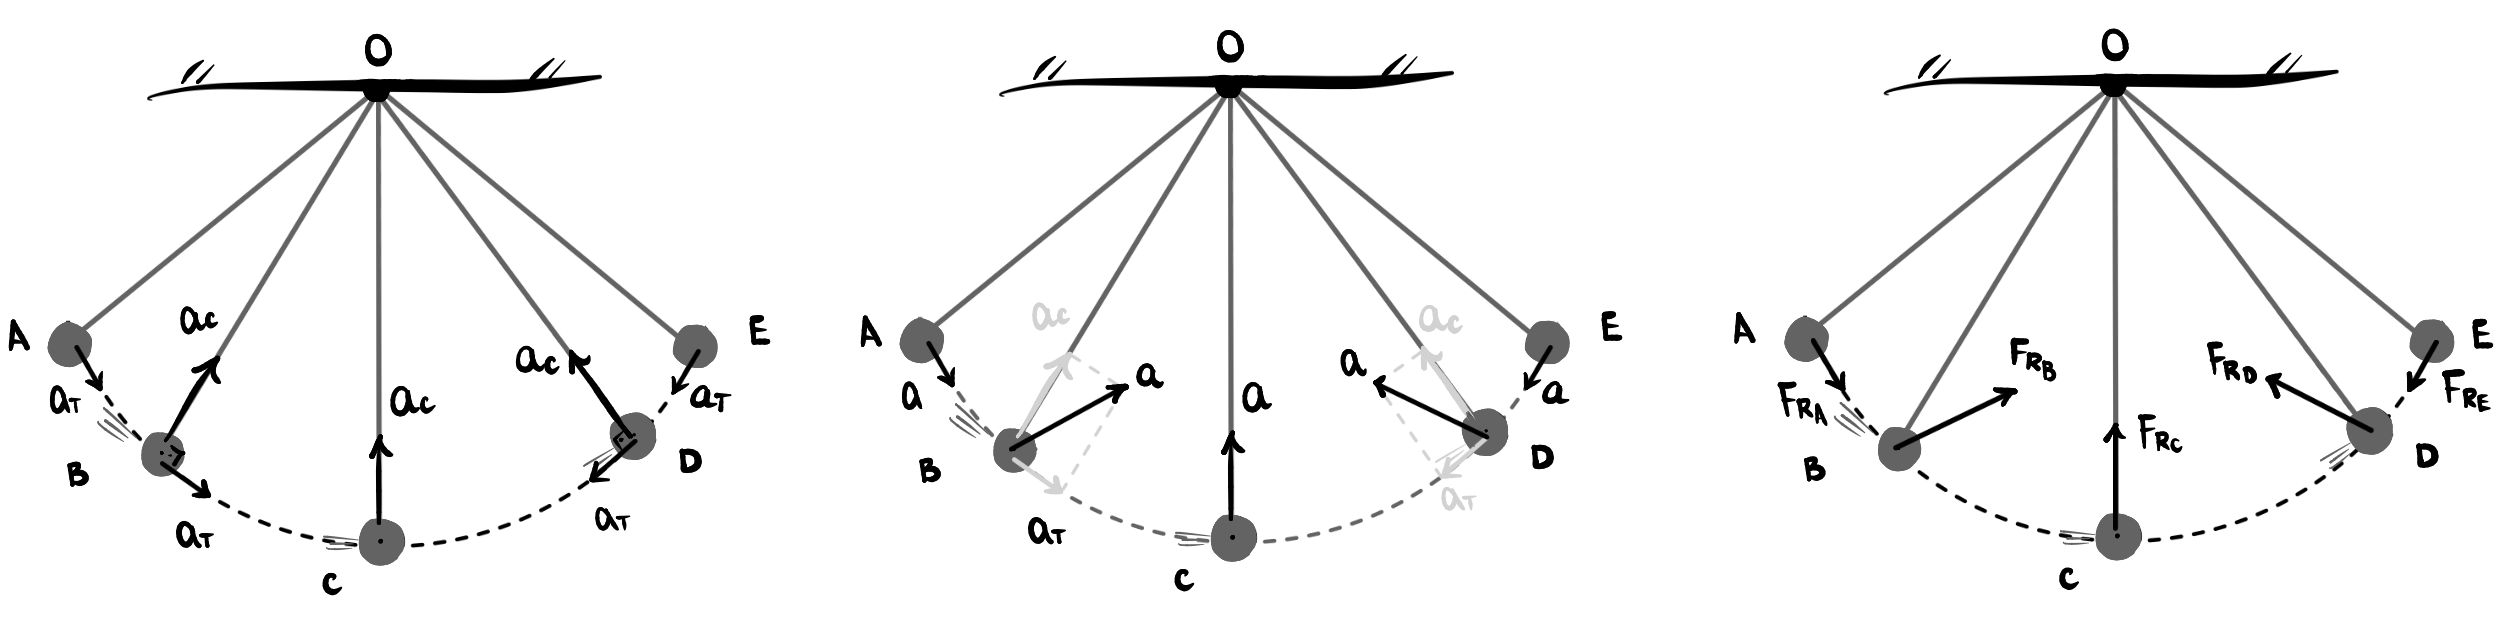
\includegraphics[width=1.0\linewidth]{imagensdinamicanewton/fcptpendulosimplesanalise3.png}};
  \end{scope}
\end{tikzpicture}
\captionof{figure}{A aceleração total e a força resultante total -- sobreposição das direções tangencial e centrípeta -- no movimento do pêndulo simples.}
\label{fig_mec_fcptpendulosimplesanalise3}
} 
\vspace{0.3cm}


A Figura \ref{fig_mec_fcptpendulosimplesanalise3} mostra tal efeito: nos pontos extremos $A$ e $E$ -- nos quais a velocidade é zero -- a força resultante é puramente tangencial, e é ela que faz com que a bolinha deixe de ter velocidade zero e passe a acelerar. No ponto $C$ -- o ponto de velocidade máxima -- a força resultante é puramente centrípeta, enquanto nos demais pontos intermediários a força resultante será uma sobreposição das componentes tangencial e centrípeta.





\vspace{0.3cm}

\begin{exemplo}[Nível I (Pêndulo Simples)]\label{exemplo_newton_frcptex01}

Para o caso do pêndulo simples de massa $m=2$kg, em um ponto em que sua velocidade vale $v=10$m/s e o fio faz um ângulo $\theta=60^\circ$ com a vertical, encontre o valor da tração no fio. O comprimento do fio é $L=4$m.


\resolucao

Como mostra a Figura \ref{fig_mec_fcptpendulosimplesanalise2}, a força resultante na direção centrípeta será

\begin{align}
         F_{\text{R}_\text{CPT}} &= F_{\text{DENTRO}} - F_{\text{FORA}}  \nonumber \\
                                 &= T - P \cos \theta \nonumber \\
                                 &= \dfrac{mv^2}{R}. \nonumber
\end{align}

Logo, para tal ponto, teremos (o raio $R$ é igual ao comprimento $L$ do fio):

$$   T = P \cos \theta + \dfrac{mv^2}{R} = 20 \cdot \dfrac{1}{2}+ \dfrac{2 \cdot 10^2}{4} \implies \boxed{T = 60 \text{ N.}}$$


\end{exemplo}

\vspace{0.3cm}

\begin{exemplo}[Nível II (Pêndulo Cônico)]\label{exemplo_newton_frcptex02}

Considere o pêndulo cônico representado na Figura \ref{fig_mec_penduloconico1}, que gira em torno do eixo vertical que passa pelo ponto O, mantendo sempre sua rotação ao longo de um mesmo plano horizontal.

\vspace{0.3cm}
 {
\centering
\begin{tikzpicture}
  \begin{scope}[blend mode=multiply]
    \node {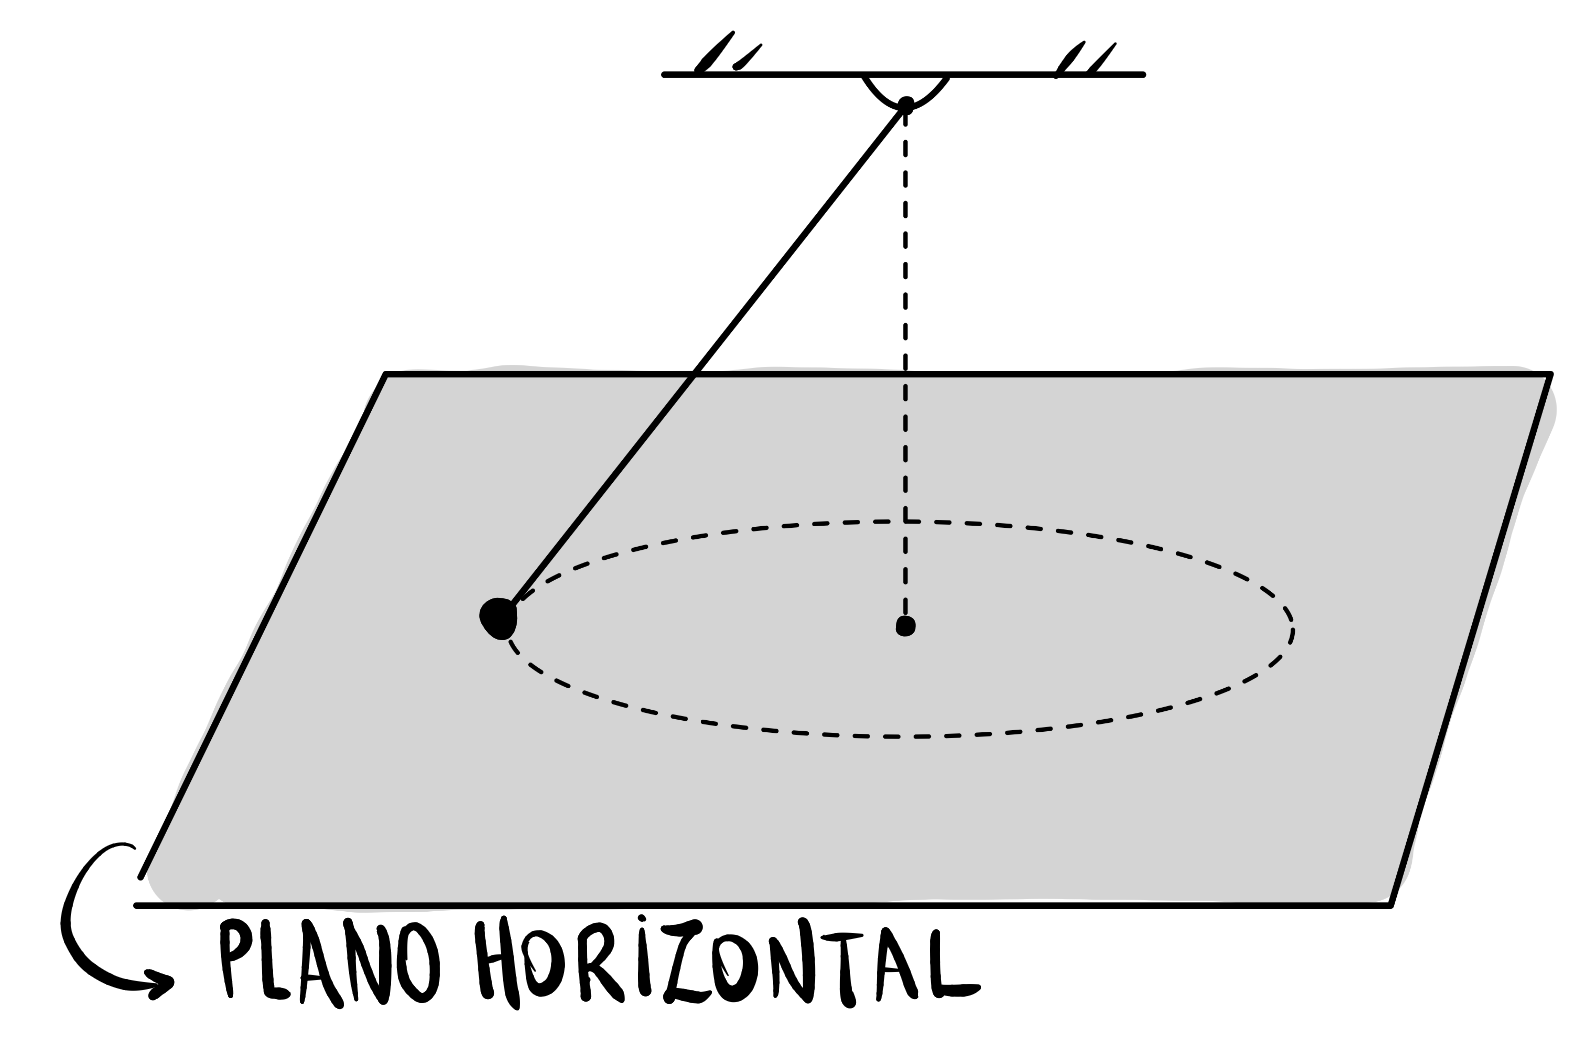
\includegraphics[width=0.35\linewidth]{imagensdinamicanewton/penduloconico2.png}};
  \end{scope}
\end{tikzpicture}
\captionof{figure}{}
\label{fig_mec_penduloconico1}
} 
\vspace{0.3cm}

Se a gravidade local vale $g$, mostre que o período $T$ do pêndulo é dado por $T= 2 \pi \sqrt{\sfrac{H}{g}},$ em que $H$ é a altura do plano de movimento da massa até o teto.

\resolucao

As forças que atuam na bolinha são a tração $T$ no fio e o seu peso $P=mg,$ como indica o primeiro desenho da Figura \ref{fig_mec_penduloconico2}. Tracemos o eixo horizontal que passa pela bolinha e também pelo centro $O$ da circunferência de sua trajetória. Sabemos que deve haver uma resultante de forças nessa direção, apontando para o centro $O,$ responsável por gerar a aceleração centrípeta $a_c.$

O outro eixo será perpendicular a este, e, portanto, será vertical. Ao decompor a tração teremos uma componente vertical $T \cos \theta$ e uma componente horizontal -- na direção centrípeta -- dada por $T \sin \theta$.

\vspace{0.3cm}
 {
\centering
\begin{tikzpicture}
  \begin{scope}[blend mode=multiply]
    \node {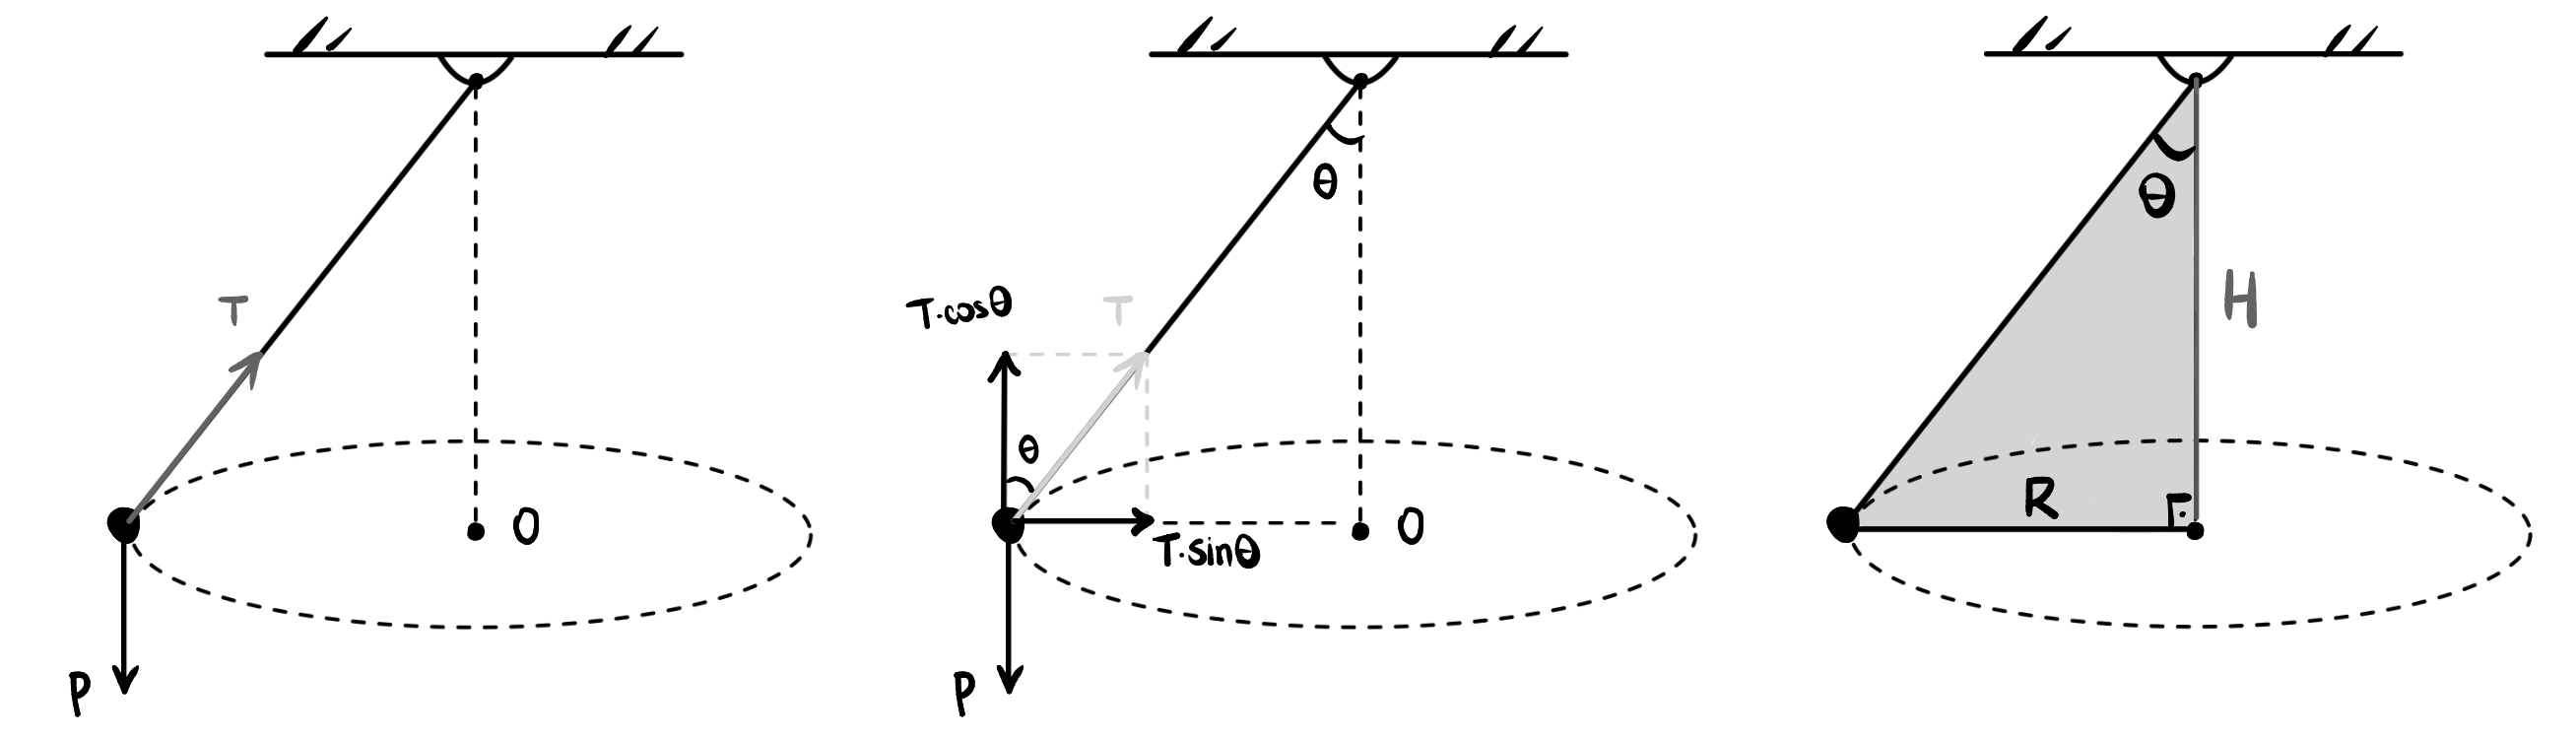
\includegraphics[width=0.85\linewidth]{imagensdinamicanewton/penduloconico1.png}};
  \end{scope}
\end{tikzpicture}
\captionof{figure}{}
\label{fig_mec_penduloconico2}
} 
\vspace{0.3cm}

Como o pêndulo gira sempre se mantendo no mesmo plano horizontal sabemos que a resultante das forças na vertical é nula -- a bolinha não possui aceleração nessa direção --, isto é:

$$ F_{\text{R}_{\text{y}}} = 0 \implies T \cos \theta = P \implies \boxed{T \cos \theta =  mg.} $$

Na direção horizontal (centrípeta) a resultante das forças deve gerar a aceleração centrípeta:

$$ F_{\text{R}_\text{CPT}} = m a_{\text{}_\text{CPT}} \implies \boxed{T \sin \theta = m \dfrac{v^2}{R}.}$$

Dividindo as duas equações obtidas acima membro a membro somos levados a

$$ \dfrac{\cancel T \sin \theta}{\cancel T \cos \theta} = \dfrac{\dfrac{\cancel mv^2}{R}}{\cancel mg} \implies \tan \theta = \dfrac{v^2}{Rg}. $$

Note que, pelo triângulo retângulo destacado na terceira imagem da Figura \ref{fig_mec_penduloconico2}, tem-se

$$ \tan \theta = \dfrac{R}{H},$$

\noindent o que, na relação anterior, fornece

$$ \tan \theta = \dfrac{v^2}{Rg} = \dfrac{R}{H} \implies v^2 = \dfrac{gR^2}{H}.$$

Note que tal valor é constante: $R$ e $H$ são parâmetros geométricos constantes e $g$ é a aceleração da gravidade -- também constante. Logo, o movimento em questão é um MCU: a velocidade, em módulo, é constante. Assim, podemos escrever que

$$ v = \dfrac{d}{t} = \dfrac{2 \pi R}{T} \implies v^2 = \dfrac{4 \pi^2 R^2}{T^2},$$

\noindent o que, na relação anterior, fornece

$$ v^2 = \dfrac{gR^2}{H} =  \dfrac{4 \pi^2 R^2}{T^2}\implies T^2 = 4 \pi^2 \dfrac{H}{g} \implies \boxed{T = 2 \pi \sqrt{ \dfrac{H}{g}}.} $$

Este é um resultado interessante: o período de oscilação do pêndulo cônico não depende do valor da massa $m$ amarrado em seu extremo -- assim como no pêndulo simples --, além de não depender do tamanho ou inclinação do fio, dependendo exclusivamente da altura $H$ entre o ponto no qual o fio é fixado e o plano horizontal de rotação da bolinha.


\end{exemplo}

\vspace{0.3cm}



\begin{exemplo}[Nível III (ITA - 1992)]\label{exemplo_newton_frcptex03}


Um aro metálico circular e duas esferas são acoplados conforme ilustra abaixo. As esferas dispõem de um furo diametral que lhes permite circular pelo aro. O aro começa a girar, a partir do repouso, em torno do diâmetro vertical $EE'$, que passa entre as esferas, até atingir uma velocidade angular constante $\omega$. 


\begin{center}
\begin{tikzpicture}[scale=0.8]

% círculo principal
\draw[thick] (0,0) circle (2);

% diâmetro vertical
\draw[dashed] (0,-2.6) -- (0,2.8);

% diâmetro horizontal
\draw[dashed] (-2.5,0) -- (2.5,0);

% eixo superior
\draw[->, thick] (0,2) -- (0,3);
\node at (0.35,2.7) {$E$};
\node at (0.35,-2.55) {$E'$};

% seta de rotação
\draw[->] (-0.7,2.4) arc[start angle=180,end angle=90,x radius=0.7,y radius=0.35];
\node at (-1.0,2.35) {$\omega$};

% pequeno aro superior
\draw (0,2.3) ellipse (0.45 and 0.12);

% raio indicado
\draw[thick,->] (0,0) -- (1.41,1.41);
\node at (0.55,0.9) {$R$};

% esferas
\fill (-0.18,-2) circle (0.12);
\fill (0.18,-2) circle (0.12);

\node at (-0.35,-1.7) {$m$};
\node at (0.35,-1.7) {$m$};

\end{tikzpicture}
\end{center}





Sendo $R$ o raio do aro, $m$ a massa de cada esfera e desprezando-se os atritos, pode afirmar que:


\begin{enumerate}
    \item [a)]as esferas permanecem na parte inferior do aro, porque esta é a posição de mínima energia potencial.

    \item [b)]as esferas permanecem a distâncias $r$ de $EE'$ tal que, se $2\theta$ for o ângulo central cujo vértice é o centro do aro e cujos lados passam pelo centro das esferas, na posição de equilíbrio estável, então $\tan \theta = \omega^2 r/g$ estando as esferas abaixo do diâmetro horizontal do aro.

    \item [c)]as esferas permanecem a distâncias $r$ de $EE'$ tal que, se $2\theta$ for o ângulo central cujo vértice é o centro do aro e cujos lados passam pelos centros das esferas, na posição de equilíbrio estável, então $\tan \theta = \omega^2 r/g$ estando as esferas acima do diâmetro horizontal do aro.

    \item [d)]As alternativas b) e c) anteriores estão corretas.

    \item [e)]A posição de maior estabilidade ocorre quando as esferas estão nos extremos de um mesmo diâmetro.
\end{enumerate}


\resolucao

A Figura \ref{fig_mec_fcptnivel3exremplo} mostra a situação do problema: a esfera estará a uma certa altura e girando em uma circunferência de raio $r$. As forças que atuam em cada esfera são o seu peso $P$ e a normal $N$ que a superfície do aro faz, que, por ser perpendicular à superfície de contato, aponta para o centro $C$ do aro.

\vspace{0.3cm}
 {
\centering
\begin{tikzpicture}
  \begin{scope}[blend mode=multiply]
    \node {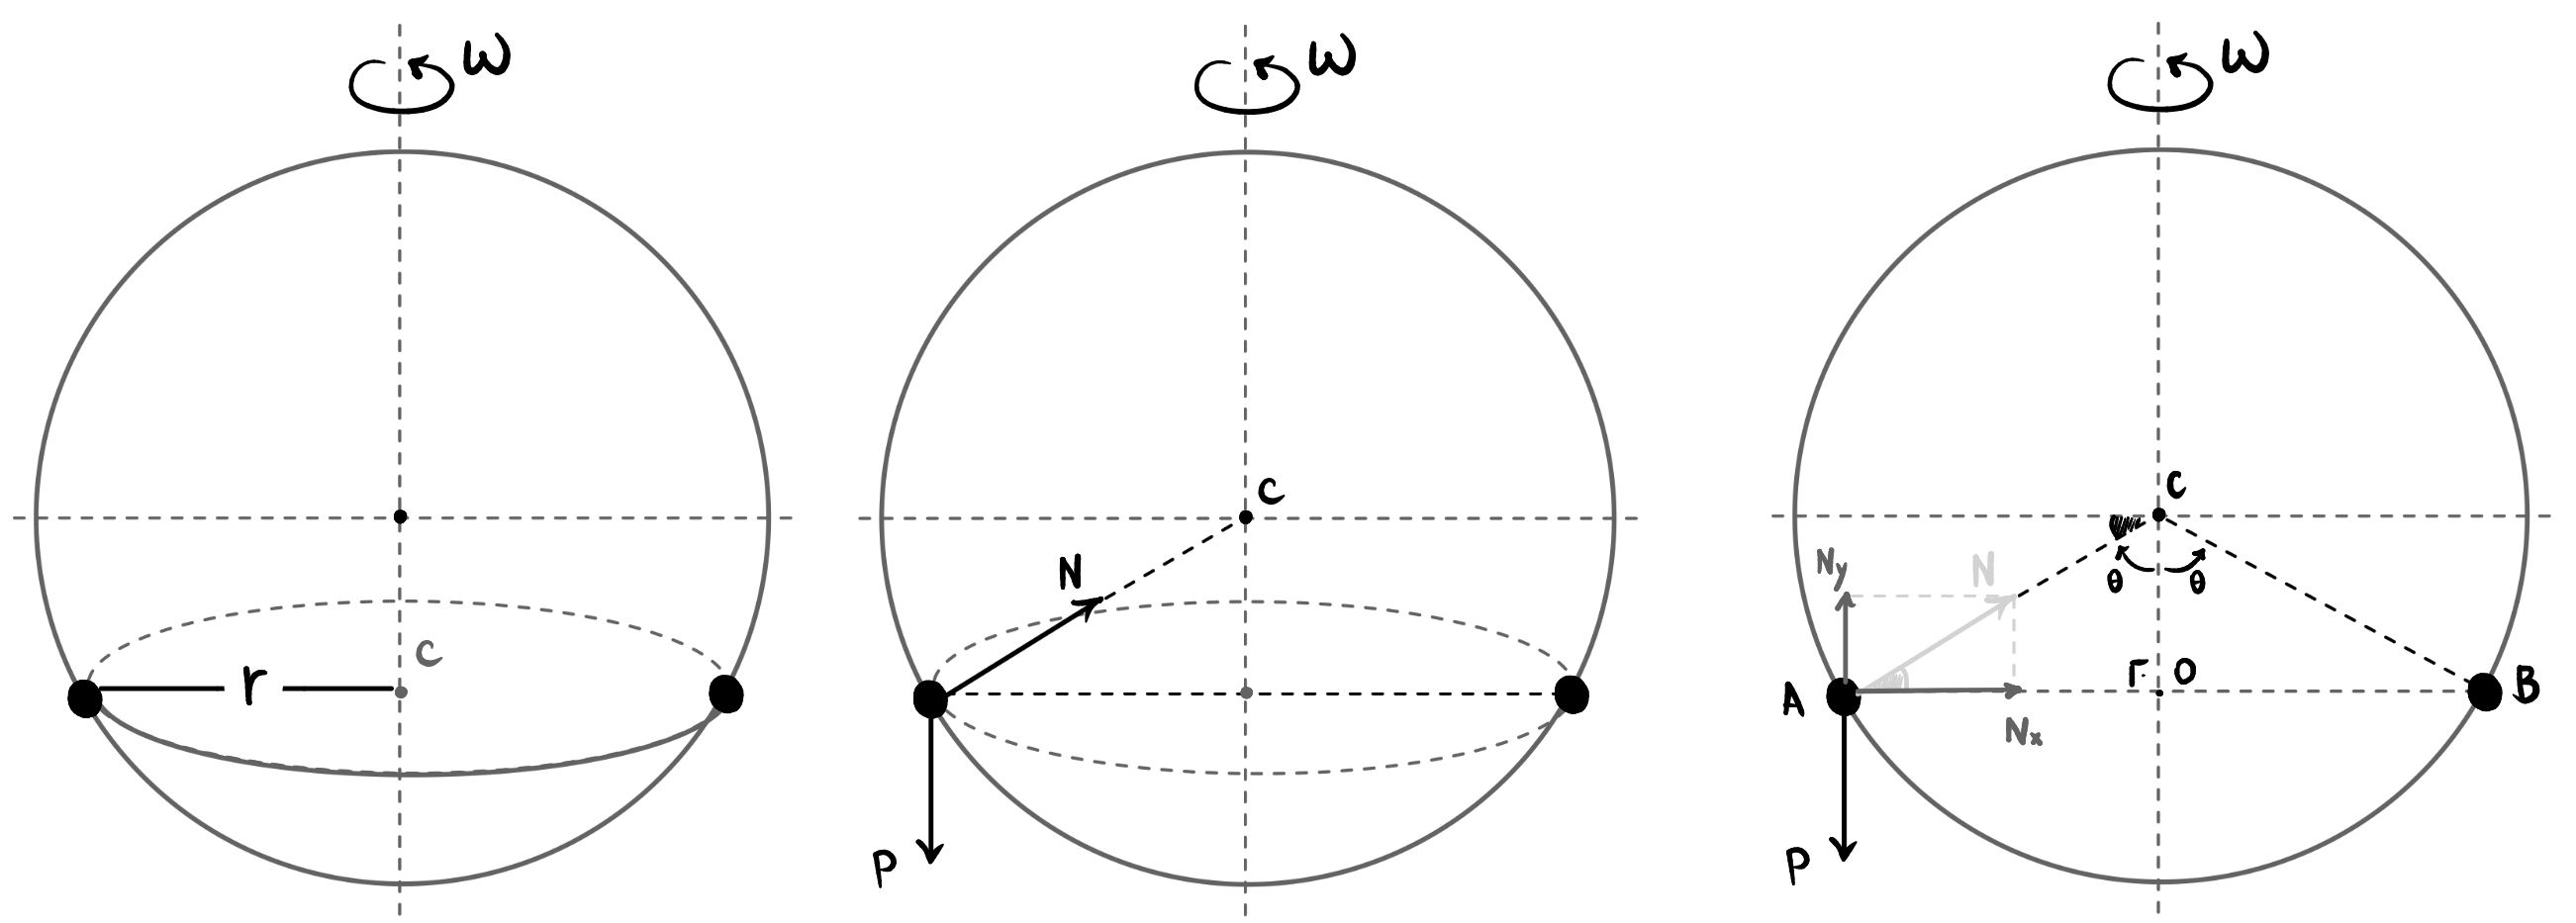
\includegraphics[width=0.85\linewidth]{imagensdinamicanewton/fcptnivel3exremplo.png}};
  \end{scope}
\end{tikzpicture}
\captionof{figure}{}
\label{fig_mec_fcptnivel3exremplo}
} 
\vspace{0.3cm}

Faremos a análise das forças para a esfera da esquerda -- para a da direita é totalmente análogo, por simetria. Deve haver uma força resultante horizontal apontado para o centro $O$ da circunferência de raio $r$: essa é a resultante centrípeta. Assim, faremos a decomposição das forças nos eixos horizontal (centrípeto) e no eixo perpendicular a este, sendo, portanto, o eixo vertical.

Na direção vertical teremos equilíbrio, dado que a esfera gira na circunferência de raio $r$ contida em um plano horizontal fixo:

$$ F_{\text{R}_{\text{y}}} = 0 \implies N_{\text{y}} = P \implies \boxed{N \cos \theta = mg.} $$

Na direção horizontal teremos a resultante centrípeta:

$$ F_{\text{R}_\text{CPT}} = m a_{\text{}_\text{CPT}} \implies N_\text{x} = m \omega^2r \implies \boxed{N \sin \theta = m \omega^2r.} $$

Dividindo as duas últimas equações obtidas, membro a membro, somos levados a

$$ \dfrac{\cancel N \sin \theta}{\cancel N \cos \theta} = \dfrac{\cancel m \omega^2 r}{\cancel m g} \implies \tan \theta = \dfrac{\omega^2r}{g}, $$

\noindent de modo que o gabarito é a letra $(b).$

Note que, para $\omega$ muito grande as bolinhas tendem a ficar na posição bem próxima dos extremos de um diâmetro, isto é:

$$ \omega \to \infty \implies \theta \to \dfrac{\pi}{2},$$

\noindent logo, vemos que as bolinhas sempre ficam abaixo do diâmetro horizontal do aro, tendendo para as posições nos extremos de tal diâmetro no limite em que $ \omega \to \infty.$



\end{exemplo}



\begin{secnivel}[Velocidade mínima no loop]{I}{Velocidade mínima para completar o loop}
  
  \eqLdois{dem}{eq_newton_velocidadeloop}{v \geq \sqrt{Rg}}

\end{secnivel}







\secgfe{De onde vem}

A Equação \eqref{eq_newton_velocidadeloop} fornece o valor da menor velocidade $v$ que um corpo deve ter para completar, sem cair, um loop circular de raio $R,$ em uma região de campo gravitacional $g$.

Tal valor refere-se ao ponto mais alto do loop: o corpo precisar ter uma velocidade pelo menos igual a $\sqrt{Rg}$ no ponto mais alto, quando estiver totalmente de cabeça para baixo, a fim de completar o loop. A Figura \ref{fig_mec_fcptloop} ilustra a situação em questão.

As duas forças que atuarão na partícula ao longo de seu movimento serão o peso -- sempre verticalmente para baixo -- e a normal entre a partícula e a superfície do loop, que é sempre perpendicular à superfície de contato e, portanto, aponta para o centro da circunferência. Sabemos que, por estar em um movimento circular, em todos os pontos deve haver uma força resultante apontando para o centro, responsável por gerar a aceleração centrípeta.

\vspace{0.3cm}
 {
\centering
\begin{tikzpicture}
  \begin{scope}[blend mode=multiply]
    \node {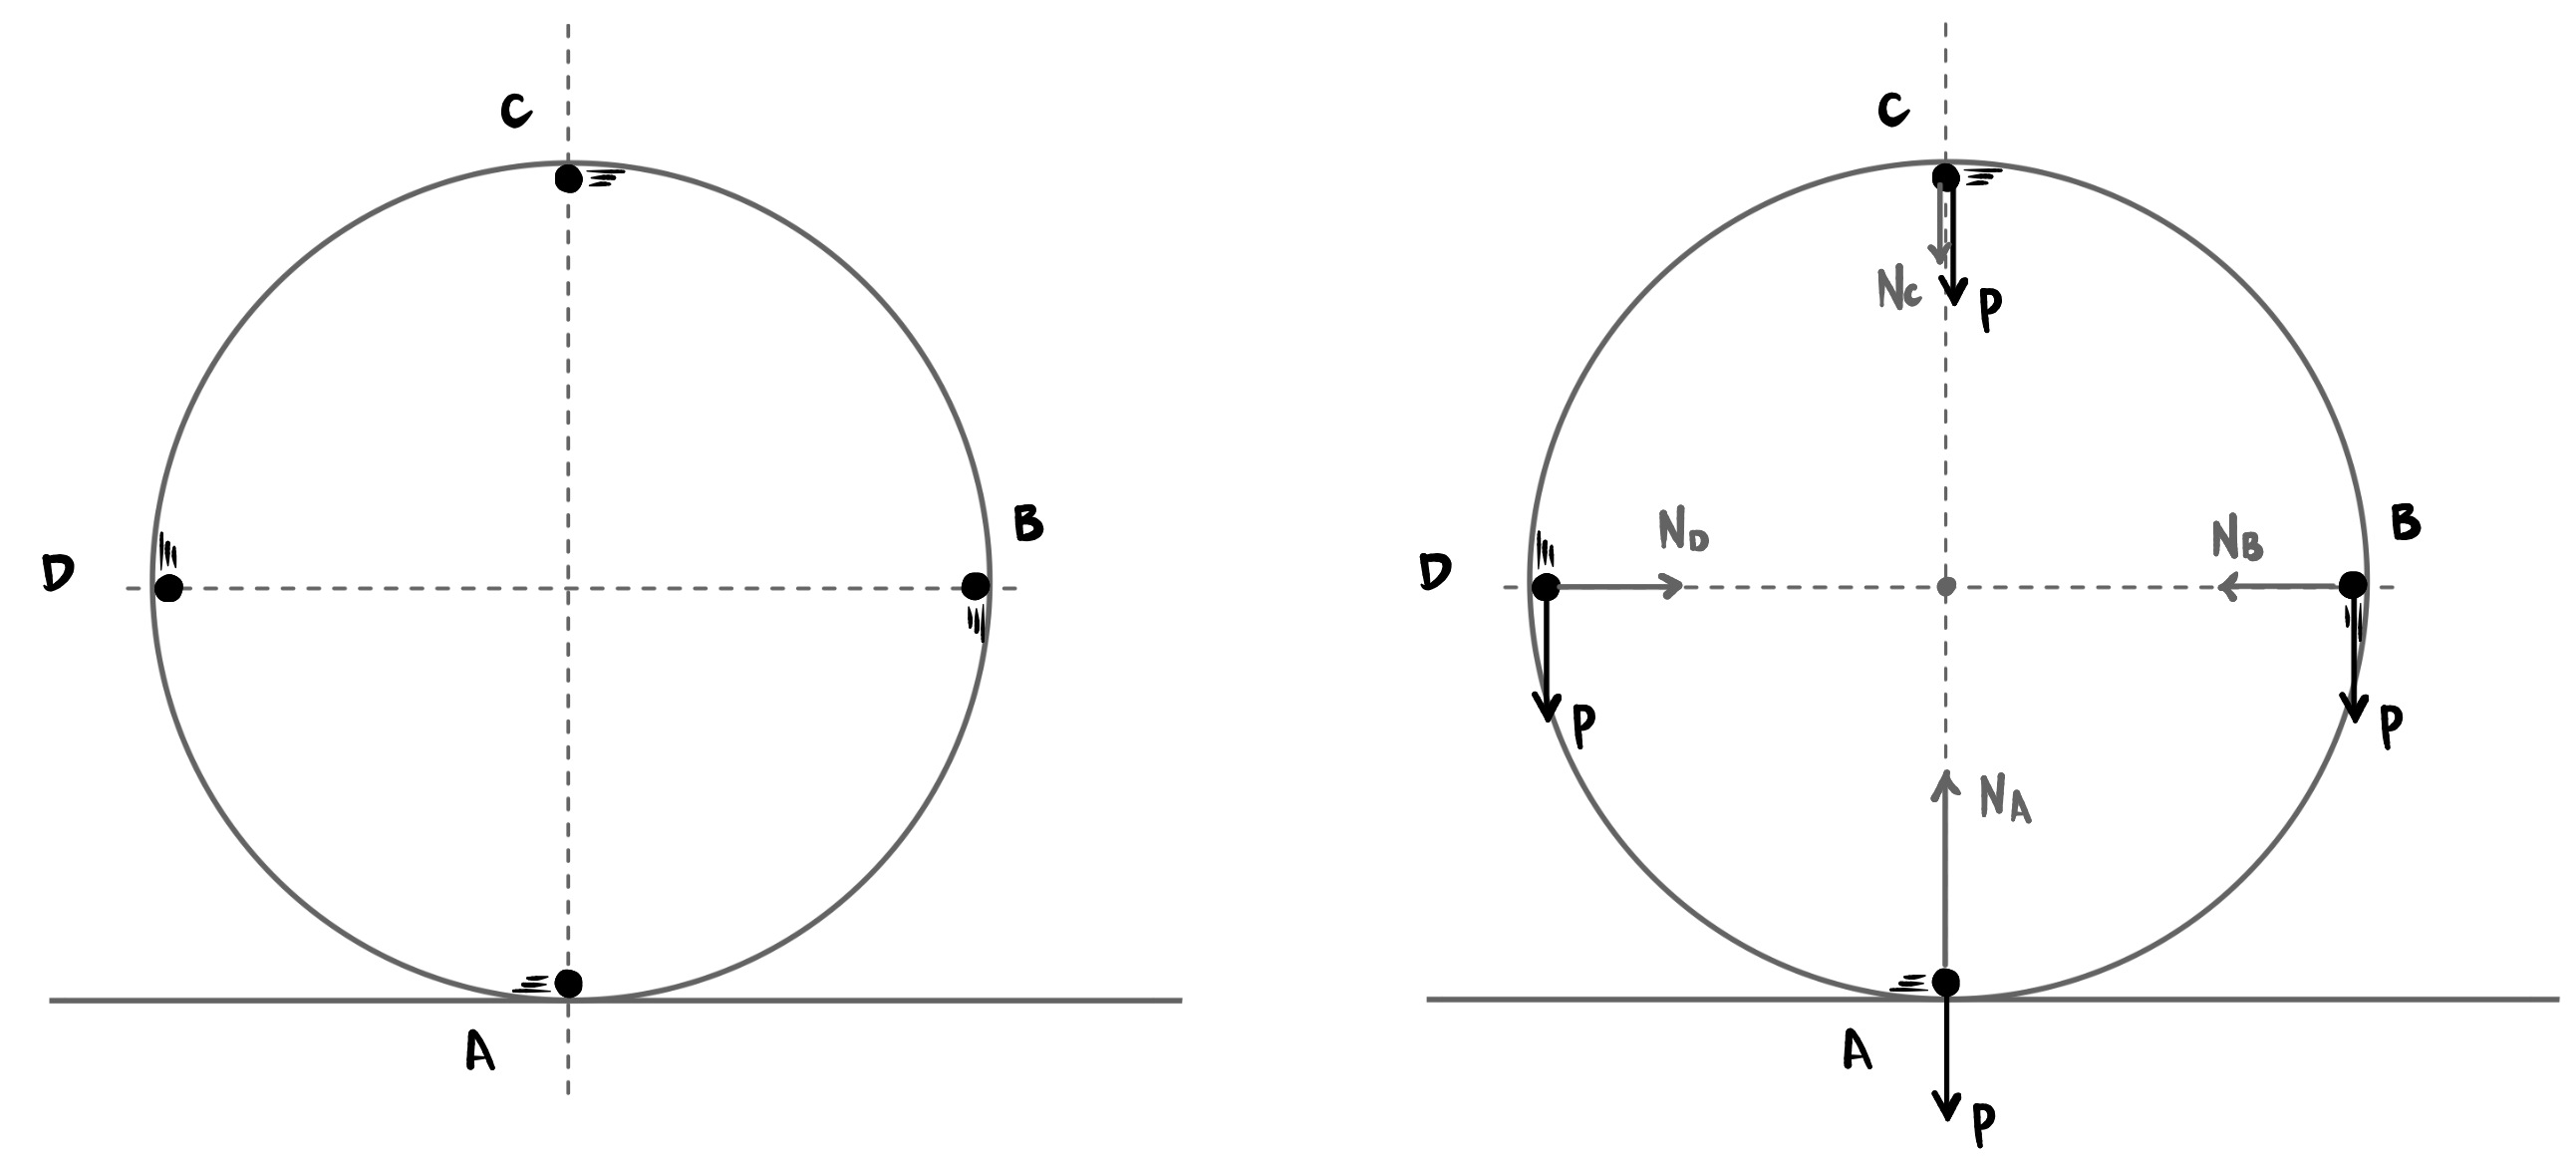
\includegraphics[width=0.85\linewidth]{imagensdinamicanewton/fcptloop.png}};
  \end{scope}
\end{tikzpicture}
\captionof{figure}{Dinâmica das forças no loop circular.}
\label{fig_mec_fcptloop}
} 
\vspace{0.3cm}

A força resultante centrípeta será dada, em todas as situações, por

$$ F_{\text{R}_\text{CPT}} = F_{\text{DENTRO}} - F_{\text{FORA}} = \dfrac{mv^2}{R}.$$

Equacionando isso para cada um dos pontos teremos:

\begin{enumerate}
    \item [(i)] Ponto mais baixo da trajetória (ponto $A)$:

    $$ F_{\text{R}_\text{CPT}} = F_{\text{DENTRO}} - F_{\text{FORA}} = N_{\text{A}} - mg =\dfrac{mv^2}{R} \implies \boxed{N_{\text{A}} = mg + \dfrac{mv^2_{\text{A}}}{R}.} $$

    \item [(ii)] Pontos $B$ ou $D:$

    $$ F_{\text{R}_\text{CPT}} = F_{\text{DENTRO}} - F_{\text{FORA}} = N_{\text{}} = \dfrac{mv^2}{R} \text{ } \begin{cases}
N_{\text{B}} = \dfrac{mv_B^2}{R} \\[8pt]
N_{\text{D}} = \dfrac{mv_D^2}{R}
\end{cases} $$

\item [(iii)] Ponto $C$, o ponto mais alto da trajetória:

 $$ F_{\text{R}_\text{CPT}} = F_{\text{DENTRO}} - F_{\text{FORA}} = N_{\text{C}} + mg =\dfrac{mv^2}{R} \implies \boxed{N_{\text{C}} =  \dfrac{mv^2_{\text{C}}}{R} - mg .} $$

 Esse é o nosso ponto crítico: o ponto no qual a partícula tem maior chance de cair. Perceba que o peso e a normal se somam, puxando a partícula para baixo. No caso limite -- em que a partícula tem, no ponto $C$, a velocidade mínima para conseguir completar o loop -- ela estará quase caindo, o que significa que a normal -- que é uma força de contato -- entre a superfície do loop e a partícula será quase zero (a partícula está quase perdendo o contato com o assoalho), logo, em tal situação limite, teríamos:

 $$  N_{\text{C}} = \dfrac{mv^2_{\text{C}}}{R} - mg \approx 0 \implies \dfrac{mv^2_{\text{C}}}{R} = mg \implies  v^2_{\text{C}} = Rg \implies \boxed{v_{\text{C}} = \sqrt{Rg}.}$$

 Tal valor é a \textbf{velocidade mínima} que a partícula deve possuir em $C$ para conseguir completar o loop -- em tal situação a partícula estará na iminência de perder o contato e começar a cair, de modo que o mais seguro é ter velocidades superiores a essa, por isso a Equação \eqref{eq_newton_velocidadeloop} representa uma desigualdade.
    
\end{enumerate}



\secgfe{Onde é usada}

O uso de tal equação é necessário para o dimensionamento de montanhas-russas que fazem loop, ou o clássico globo da morte dos circos, em que um motociclista entra em uma esfera e completa o loop de moto.



\secgfe{Erros comuns}

O erro mais comum aqui é o estudante se ater a memorizar a Equação \eqref{eq_newton_velocidadeloop} sem entender o que de fato está por trás dela. O fato mais relevante aqui é compreender todos os passos no desenvolvimento de tal equação: o diagrama de forças, a condição de iminência de perder o contato com o assoalho (normal tender a zero) e o equacionamento da resultante centrípeta. Saber construir todos os passos desse raciocínio é a parte importante e o trabalho a ser feito -- memorizar a fórmula se torna dispensável para quem o sabe.



\secgfe{Observações}

Talvez o leitor ache estranho, em um primeiro momento, o fato de que, no ponto de altura máxima, existem duas forças puxando a partícula diretamente para baixo e, ainda assim, a partícula não cai. Acontece que ela cai -- só não como o leitor espera. Observe a Figura \ref{fig_mec_loopobs1} que mostra dois corpos sob a ação do campo gravitacional. O da direita é abandonado do repouso, e cai em linha reta, enquanto o da esquerda possui uma velocidade inicial. 

Se formos avaliar no ponto mais alto da trajetória do primeiro corpo, as forças que nele atuam são exatamente iguais às forças que atuam no corpo que foi abandonado: apenas o seu peso, que atua na vertical, dirigido para baixo. Ora, se é assim, porque a primeira partícula não cai a partir do seu ponto de altura máxima? Acontece que ela cai, contudo, por já ter uma velocidade inicial (para a horizontal, no caso) ela não cai simplesmente em linha reta, como a bolinha da direita: ela cai enquanto continua se movendo para a direita, por conta de sua velocidade. Assim, ao longo de tal queda, a partícula descreverá uma trajetória parabólica.

\vspace{0.3cm}
 {
\centering
\begin{tikzpicture}
  \begin{scope}[blend mode=multiply]
    \node {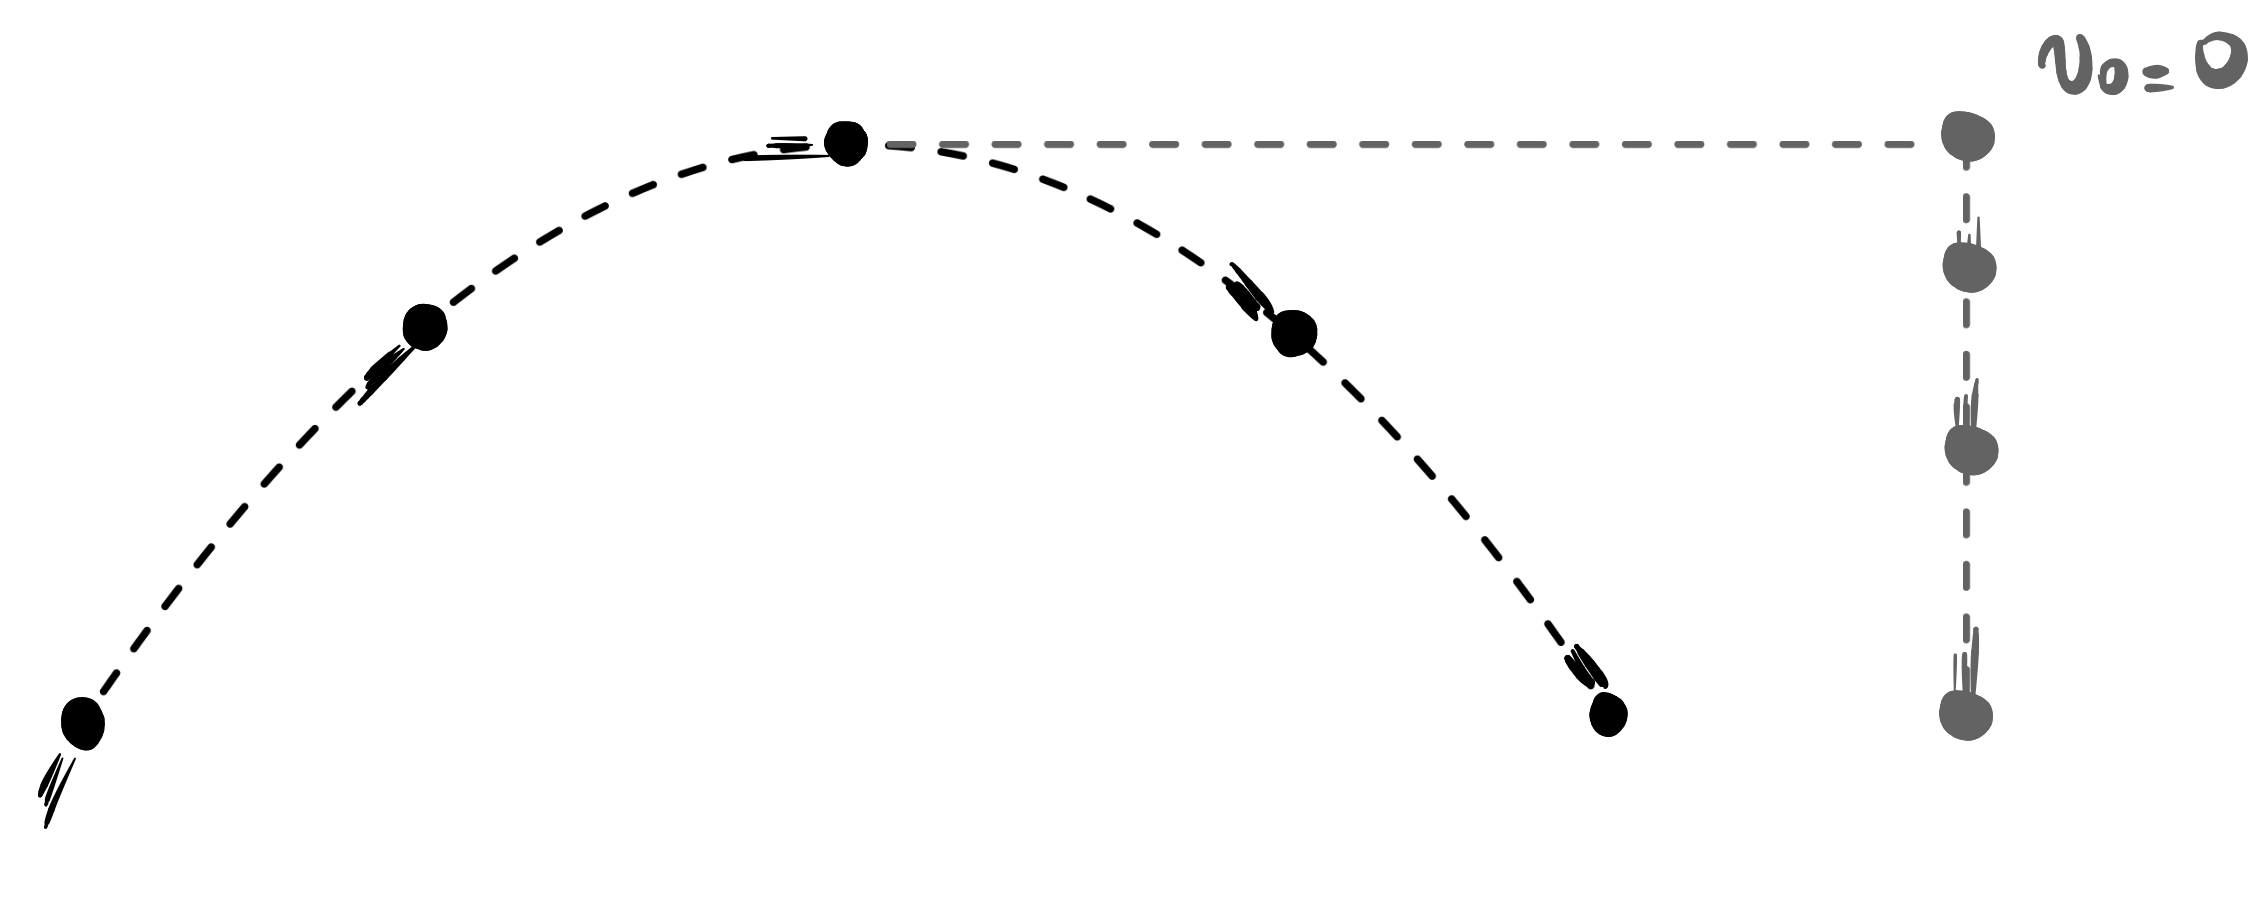
\includegraphics[width=0.6\linewidth]{imagensdinamicanewton/loopobs1.png}};
  \end{scope}
\end{tikzpicture}
\captionof{figure}{Dois corpos caindo sob a ação da gravidade: um possui trajetória parabólica e o outro trajetória retilínea.}
\label{fig_mec_loopobs1}
} 
\vspace{0.3cm}

Logo, é preciso haver uma certa harmonia entre cair (ação da gravidade) e mover-se na direção perpendicular à de queda (ação inercial por conta da velocidade do corpo) a fim de que o corpo descreva exatamente a trajetória da parábola em questão. Algo parecido ocorre com a partícula no loop, no ponto mais alto de sua trajetória, como tenta ilustrar a Figura \ref{fig_mec_loopobs2}.

Em tal figura, tentamos mostrar que a partícula que descreve o loop (circunferência), no seu ponto mais alto, tem um movimento semelhante ao da partícula no movimento parabólico: ela cai, porém não cai em linha reta, uma vez que, por ter a velocidade exata da Equação \eqref{eq_newton_velocidadeloop}, ela consegue achar o exato equilíbrio entre cair e se mover horizontalmente, de modo a permanecer na trajetória circular, assim como a partícula da Figura \ref{fig_mec_loopobs1} consegue fazê-lo para se manter na trajetória parabólica.

\vspace{0.3cm}
 {
\centering
\begin{tikzpicture}
  \begin{scope}[blend mode=multiply]
    \node {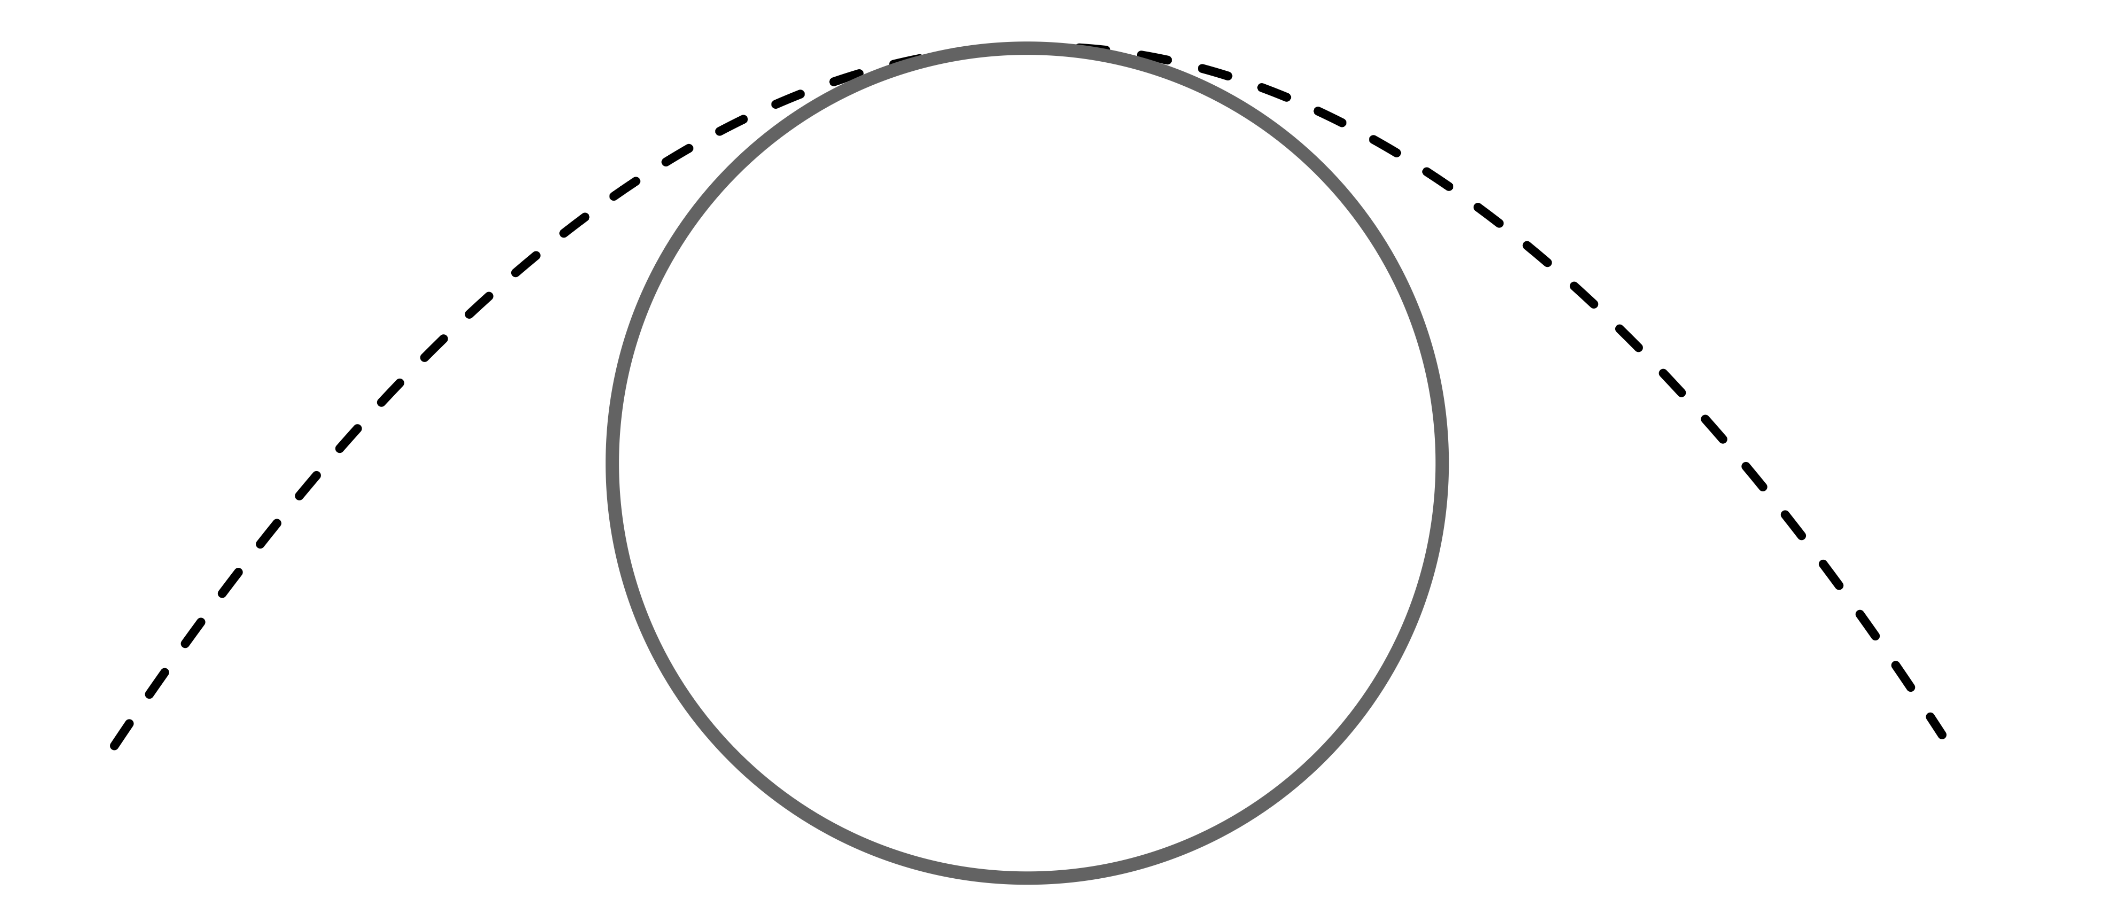
\includegraphics[width=0.4\linewidth]{imagensdinamicanewton/loopobs2.png}};
  \end{scope}
\end{tikzpicture}
\captionof{figure}{O movimento do loop é semelhante ao movimento parabólico do projétil.}
\label{fig_mec_loopobs2}
} 
\vspace{0.3cm}

O intuito desta seção, como dito, é trazer um pouco mais de intuição ao leitor e tentar sanar, quem sabe, algumas dúvidas que possam ter surgido. Iremos discorrer com muito mais profundidade sobre este assunto no estudo da Equação \eqref{eq_gravitacao_velocidadeorbital}. Esbarraremos por lá em um problema bem semelhante a este: se a Terra é atraída pelo sol pela força gravitacional, por que ela não cai no sol?

\vspace{0.3cm}

\begin{exemplo}[Nível I]\label{exemplo_newton_vloopex01}

Qual é a menor velocidade que uma partícula deve ter a fim de completar um loop de raio $R=3.6$m sem cair? A gravidade local vale $g=10$ m/s$^2$.

\resolucao

A solução consiste na aplicação direta da Equação \eqref{eq_newton_velocidadeloop}. Não recomendo, contudo, que o leitor faça uso tão imediato desse atalho sem antes ter deduzido a referida equação algumas vezes — cinco serão suficientes para formar caráter matemático. O autor já atravessou esse purgatório algébrico, razão pela qual se permite, aqui, certa economia de esforços. 

Indo às vias de fato, teremos:

$$ v_{\text{MIN}} = \sqrt{Rg} = \sqrt{3.6 \cdot 10} \implies \boxed{v_{\text{MIN}} =6 \text{ m/s}.} $$


É importante notar que essa é a menor velocidade necessária de se ter no ponto mais alto da trajetória. É possível entrar no loop com este valor de velocidade e mantê-lo constante ao longo de todo o movimento, o que possibilitaria concluir com sucesso a tarefa. De outro modo, é possível também entrar no loop com uma velocidade maior ou menor do que $6$ m/s, e ir ajustando a velocidade -- diminuindo ou aumentando -- de modo a chegar no ponto de altura máxima com tal valor de velocidade.

\end{exemplo}


\vspace{0.3cm}



\begin{exemplo}[Nível II]\label{exemplo_newton_vloopex02}

Um engenheiro de segurança projeta o loop de uma montanha-russa de raio $R = 10\,\text{m}$.
Para garantir que os passageiros sintam contato com o assento mesmo no ponto mais
alto --- e não flutuem como astronautas ---, ele exige que o carro passe pelo topo com
velocidade igual ao \emph{dobro} da velocidade mínima: $v_{\text{topo}} = 2\,v_\text{min}$.
A massa total do carro com passageiros é $m = 500\,\text{kg}$.
 
Calcule a força normal que a pista exerce sobre o carro no topo do loop nessa condição.

\resolucao
 
Calculamos primeiro $v_\text{min}$:
%
\[
    v_\text{min} = \sqrt{Rg} = \sqrt{10 \cdot 10} = 10\,\text{m/s.}
\]
%
Logo, $v_{\text{topo}} = 2 \cdot 10 = 20\,\text{m/s}$.
Aplicando a Segunda Lei de Newton na direção centrípeta no topo do loop ---
onde $N$ e $P$ apontam ambos para o centro da circunferência:
%
\[
    N + mg \;=\; \frac{m\,v_{\text{topo}}^{2}}{R}
           \;=\; \frac{500 \cdot 400}{10}
           \;=\; 20\,000\,\text{N.}
\]
%
Isolando $N$:
%
\[
    N \;=\; 20\,000 - mg
      \;=\; 20\,000 - 500 \cdot 10
      \;=\; 20\,000 - 5\,000
      \;=\; \boxed{15\,000\,\text{N.}}
\]
 
Observe que $N = 3\,mg$.
De fato, é possível mostrar que, para $v_{\text{topo}} = n\,v_\text{min}$, a normal no topo é
sempre $N = (n^{2} - 1)\,mg$ --- resultado que o leitor pode verificar
algebricamente por si mesmo, substituindo $v = n\sqrt{Rg}$ na equação centrípeta
acima.
A exigência do engenheiro de duplicar a velocidade mínima multiplica a força normal
por um fator de três em relação ao peso --- o que impõe requisitos estruturais
consideráveis à pista e ao trilho.




\end{exemplo}

\vspace{0.3cm}




\begin{exemplo}[Nível III]\label{exemplo_newton_vloopex02}

Uma bola é chutada horizontalmente com velocidade $v_0$ a partir do topo de um hemisfério de raio $R$. Determine a menor velocidade $v_0$ para que a bola nunca mais toque o hemisfério após o lançamento.


\resolucao

Faremos duas soluções para este problema: uma dinâmica e a outra, cinemática.


\sepsolucao{Solução I \,---\, Dinâmica: Condição de Desprendimento}

A Figura \ref{fig_mec_loopobs2} já ilustra, de certo modo, parte da nossa situação. A trajetória do corpo lançado será uma parábola -- pontilhada na figura em questão -- e, no ponto mais alto do hemisfério, a parábola é tangente a ele. No nosso caso, a trajetória seria apenas a metade direita da parábola: do ponto de lançamento da bola em diante.

\medskip

Contudo, por simetria temporal --- as leis de Newton
não distinguem passado de futuro --- essa parábola pode ser lida por completo, considerando sua metade esquerda, como sendo a trajetória de uma bola lançada do solo que atinge o topo do hemisfério no pico
de sua trajetória, passando por ele. Nesse ponto de altura máxima a bola tem velocidade puramente horizontal $v_0$
e move-se em uma trajetória que, instantaneamente, é circular de raio $R$. A resultante centrípeta aponta para baixo, em direção ao centro da esfera:

$$ mg - N = \frac{mv_0^2}{R} \implies N = m\!\left(g - \frac{v_0^2}{R}\right). $$

Se $N > 0$: o hemisfério empurra a bola para cima --- ela \textit{está} pressionando
a superfície e a parábola penetra no hemisfério. Se $N = 0$: a bola é lançada do solo e passa exatamente
\textit{beijando} o topo, sem pressionar. Se $N < 0$: a superfície precisaria puxar
a bola, o que é impossível --- a parábola já não alcança o hemisfério. O limiar é:

$$ N = 0 \implies \boxed{v_{0,\min} = \sqrt{gR}.} $$

Resta verificar que, com $v_0 = \sqrt{gR}$, a parábola não reencontra o hemisfério
nos flancos. Com essa velocidade, a parábola tem raio de curvatura $R$ exatamente
no topo --- igual ao do hemisfério. Mas a curvatura da parábola decresce para os
lados, como mostra a própria Figura \ref{fig_mec_loopobs2}, enquanto a do hemisfério permanece $R$: as duas curvas se tangenciam no topo
e divergem imediatamente após. Os flancos não oferecem perigo.

\sepsolucao{Solução II \,---\, Cinemática: decomposição do lançamento}

Com origem no centro da base, a trajetória a partir do topo $(0,R)$ é

$$ x = v_0 t, \qquad y = R - \tfrac{1}{2}gt^2. $$

A condição $x^2 + y^2 \geq R^2$ para todo $t > 0$ expande para

$$ t^2\!\left(v_0^2 - gR + \tfrac{1}{4}g^2t^2\right) \geq 0. $$

Para $t > 0$ o mínimo da expressão entre parênteses ocorre em $t = 0$, valendo
$v_0^2 - gR$. Basta então $v_0^2 \geq gR$:

$$ \boxed{v_{0,\min} = \sqrt{gR}.} $$

A Solução~I diz o porquê: abaixo de $\sqrt{gR}$ a parábola penetra o hemisfério
no topo; exatamente em $\sqrt{gR}$ ela o beija e diverge. A Solução~II confirma
algebricamente que a parábola fica fora para toda a trajetória.

\end{exemplo}
\vspace{0.3cm}




\begin{secnivel}[Velocidade mínima para fazer curva]{II}{Velocidade mínima para fazer uma curva em uma estrada horizontal}
  
  \eqLdois{dem}{eq_newton_velocidademinimaparacurva}{v = \sqrt{\mu_e Rg}}

\end{secnivel}






\secgfe{De onde vem}

Considere um carro se movendo em um plano horizontal, com velocidade de módulo constante, realizando uma curva de raio $R.$ O coeficiente de atrito estático entre os pneus e o solo é igual a $\mu_e$ e a gravidade local vale $g.$

A primeira imagem da Figura \ref{fig_mec_fcptcurva01} mostra qual é a tendência de movimento do carro, caso não houvesse uma resultante de forças apontando para o centro. Note que, por inércia, a tendência do carro é se mover em linha reta, em movimento uniforme. Assim, ele tende a se mover para aonde aponta sua velocidade -- na direção da tangente -- e, caso não houvesse nenhuma resultante de forças apontando para o centro, ele se moveria em linha reta da posição $A$ para a posição $B$, em um intervalo, digamos, de $1$ segundo.

\vspace{0.3cm}
 {
\centering
\begin{tikzpicture}
  \begin{scope}[blend mode=multiply]
    \node {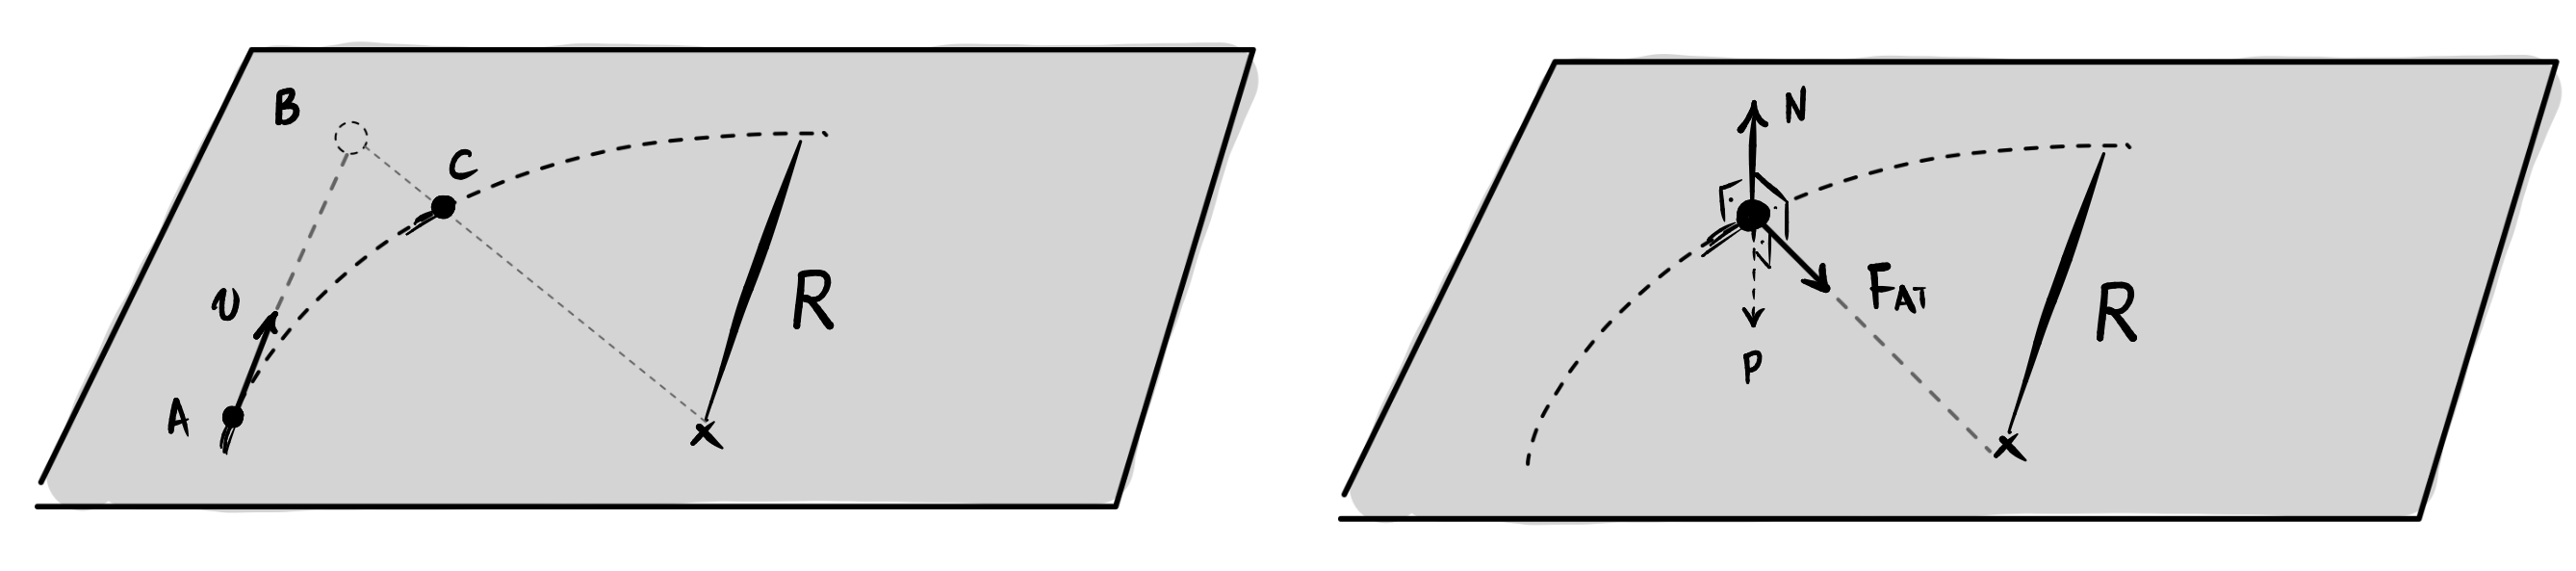
\includegraphics[width=0.9\linewidth]{imagensdinamicanewton/fcptcurva1.png}};
  \end{scope}
\end{tikzpicture}
\captionof{figure}{Análise da dinâmica de um carro em curva em um plano horizontal.}
\label{fig_mec_fcptcurva01}
} 
\vspace{0.3cm}



Neste mesmo intervalo de tempo, na trajetória curvilínea, o carro se moveria de $A$ para $C$. É fácil perceber que a diferença entre a posição do carro na trajetória curva (ponto $C)$ e a posição que o carro estaria caso não houvesse forças alterando seu movimento (ponto $B)$: o carro tende a sair para fora da curva. Assim, a força de atrito, que contraria essa tendência de movimento, atuaria apontando para o centro da curva: é ela que atuará como resultante centrípeta.

Fazendo a análise das forças que atuam no carro vemos que, pelo plano de movimento ser horizontal, as forças se anulam na vertical:

$$ F_{\text{R}_{\text{y}}} = 0 \implies N = P=mg.$$

Já na direção radial temos a força de atrito atuando como resultante centrípeta:

$$ F_{\text{R}_{\text{CPT}}} = F_{\text{AT}} = \dfrac{mv^2}{R}.$$

Usando a Equação \eqref{eq_newton_fatestatico} podemos escrever a desigualdade

$$ F_{\text{AT}_\text{EST}} \leq \mu_e N$$

\noindent e, pelas duas equações anteriores, temos

$$  \dfrac{mv^2}{R} \leq \mu_emg \implies v^2 \leq \mu_e R g \implies \boxed{v \leq \sqrt{\mu_e R g },}  $$

\noindent ou seja, a velocidade máxima que o carro pode ter na curva para não derrapar (não romper o regime de atrito estático e entrar no regime de atrito cinético) é aquela para a qual a força de atrito está no seu limite: o atrito é o estático máximo. Tal velocidade é aquela para qual temos uma igualdade na desigualdade acima, ou seja

$$ v_{\text{max}} =\sqrt{\mu_e R g }, $$

\noindent como queríamos demonstrar.


\secgfe{Onde é usada}


A Equação \eqref{eq_newton_velocidademinimaparacurva} é, na verdade, apenas uma aplicação das leis de Newton para movimentos curvilíneos. Perceba que ela foi obtida exatamente pela aplicação direta das Equações\eqref{eq_newton_fatestatico} e \eqref{eq_newton_forcacentripeta}.

Assim, tal equação é usada, de forma explícita, apenas no contexto de se computar a máxima velocidade com que um carro pode fazer uma curva em um plano horizontal. Contudo, o raciocínio para construí-la possui diversas aplicações, e é em sua construção que o leitor deve se atentar -- e não em apenas memorizar a equação em si.



\secgfe{Erros comuns}

Uma confusão comum aqui é o aluno pensar que, pelo fato do carro estar em movimento, o atrito que atua é o cinético, o que causa uma certa incoerência com o fato do coeficiente de atrito que aparece na Equação \eqref{eq_newton_velocidademinimaparacurva} ser o estático.

Acontece que este raciocínio está equivocado: o atrito que atua no carro, caso ele se mova sem derrapar, é o atrito estático. Isso porque, apesar de o carro estar em movimento, no movimento sem derrapagem o ponto do pneu em contato com o solo fica momentaneamente em repouso. Com isso, não há movimento relativo entre as superfícies (o ponto do pneu em contato com a estrada e a estrada) de modo que o atrito que atua é o estático.

Essa discussão foi feita no estudo da Equação \eqref{eq_newton_fatcinetico}, durante a exposição sobre o funcionamento do freio ABS. Recomendamos ao leitor que ficou com essa dúvida que revisite tal seção para clarear este conceito.




\secgfe{Observações}

Uma análise rápida da Equação \eqref{eq_newton_velocidademinimaparacurva} nos permite concluir que

\begin{enumerate}
    \item [(i)] em curvas muito fechadas (pequeno raio $R$ de curvatura) a velocidade máxima com que se pode entrar nelas é menor. 

    A velocidade máxima na curva é diretamente proporcional à raiz quadrada do raio de curvatura $R$. Isso faz com que, em curvas fechadas, seja necessário maior força centrípeta, o que exigiria mais atrito. É por isso que nas estradas sempre há avisos quando se está aproximando de uma curva fechada: é importante diminuir a velocidade nesses trechos a fim de que não corra risco do carro derrapar (o atrito estático atingir o máximo, rompendo o regime de atrito estático para cinético) ou sair da curva.

    \item [(ii)] em dias chuvosos ou em caso de óleo na pista a maior velocidade com que se pode fazer a curva também diminui. Isso porque a Equação \eqref{eq_newton_velocidademinimaparacurva} indica que a velocidade máxima na curva é diretamente proporcional ao coeficiente de atrito estático $\mu_e$ entre os pneus e o asfalto. Contudo, se o asfalto estiver molhado ou com óleo na pista teremos uma superfície mais lisa/escorregadia, o que faz o coeficiente de atrito diminuir e, consequentemente, diminui-se a máxima velocidade que se pode ter para fazer tal curva.
\end{enumerate}




\vspace{0.3cm}


\begin{exemplo}[Nível I]\label{exemplo_newton_velocidademinimacurvahorizontalex01}

Um carro entra em uma curva, em uma pista horizontal, de raio $R=180$ m. Se ele entra com velocidade $v=120$ km/h e o coeficiente de atrito estático entre os pneus e o solo vale $\mu_e=0.5,$ é possível que ele realize a curva em segurança?

\resolucao

A Equação \eqref{eq_newton_velocidademinimaparacurva} nos diz que a máxima velocidade que esse carro pode ter para realizar a curva sem derrapar é

$$ v=\sqrt{\mu_e R g} = \sqrt{0.5 \cdot 180 \cdot 10} = 30 \text{m/s} = 108 \text{ km/h},$$

\noindent ou seja, para velocidades maiores que 108 km/h a força centrípeta exigida seria maior do que aquela que o atrito estático máximo consegue oferecer, entrando em regime de atrito cinético e causando derrapagem. Logo, para qualquer valor de velocidade acima de 108 km/h o carro não fará a curva em segurança, incorrendo em derrapagens pela ação do atrito cinético, que é o caso do contexto proposto para a velocidade de 120 km/h.

\end{exemplo}


\vspace{0.3cm}


\begin{exemplo}[Nível II]\label{exemplo_newton_velocidademinimacurvahorizontalex02}

Considere uma pista circular, inclinada de ângulo $\theta$ em relação à horizontal, como mostra a Figura \ref{fig_mec_fcptcurva02}.

 \vspace{0.3cm}
 {
\centering
\begin{tikzpicture}
  \begin{scope}[blend mode=multiply]
    \node {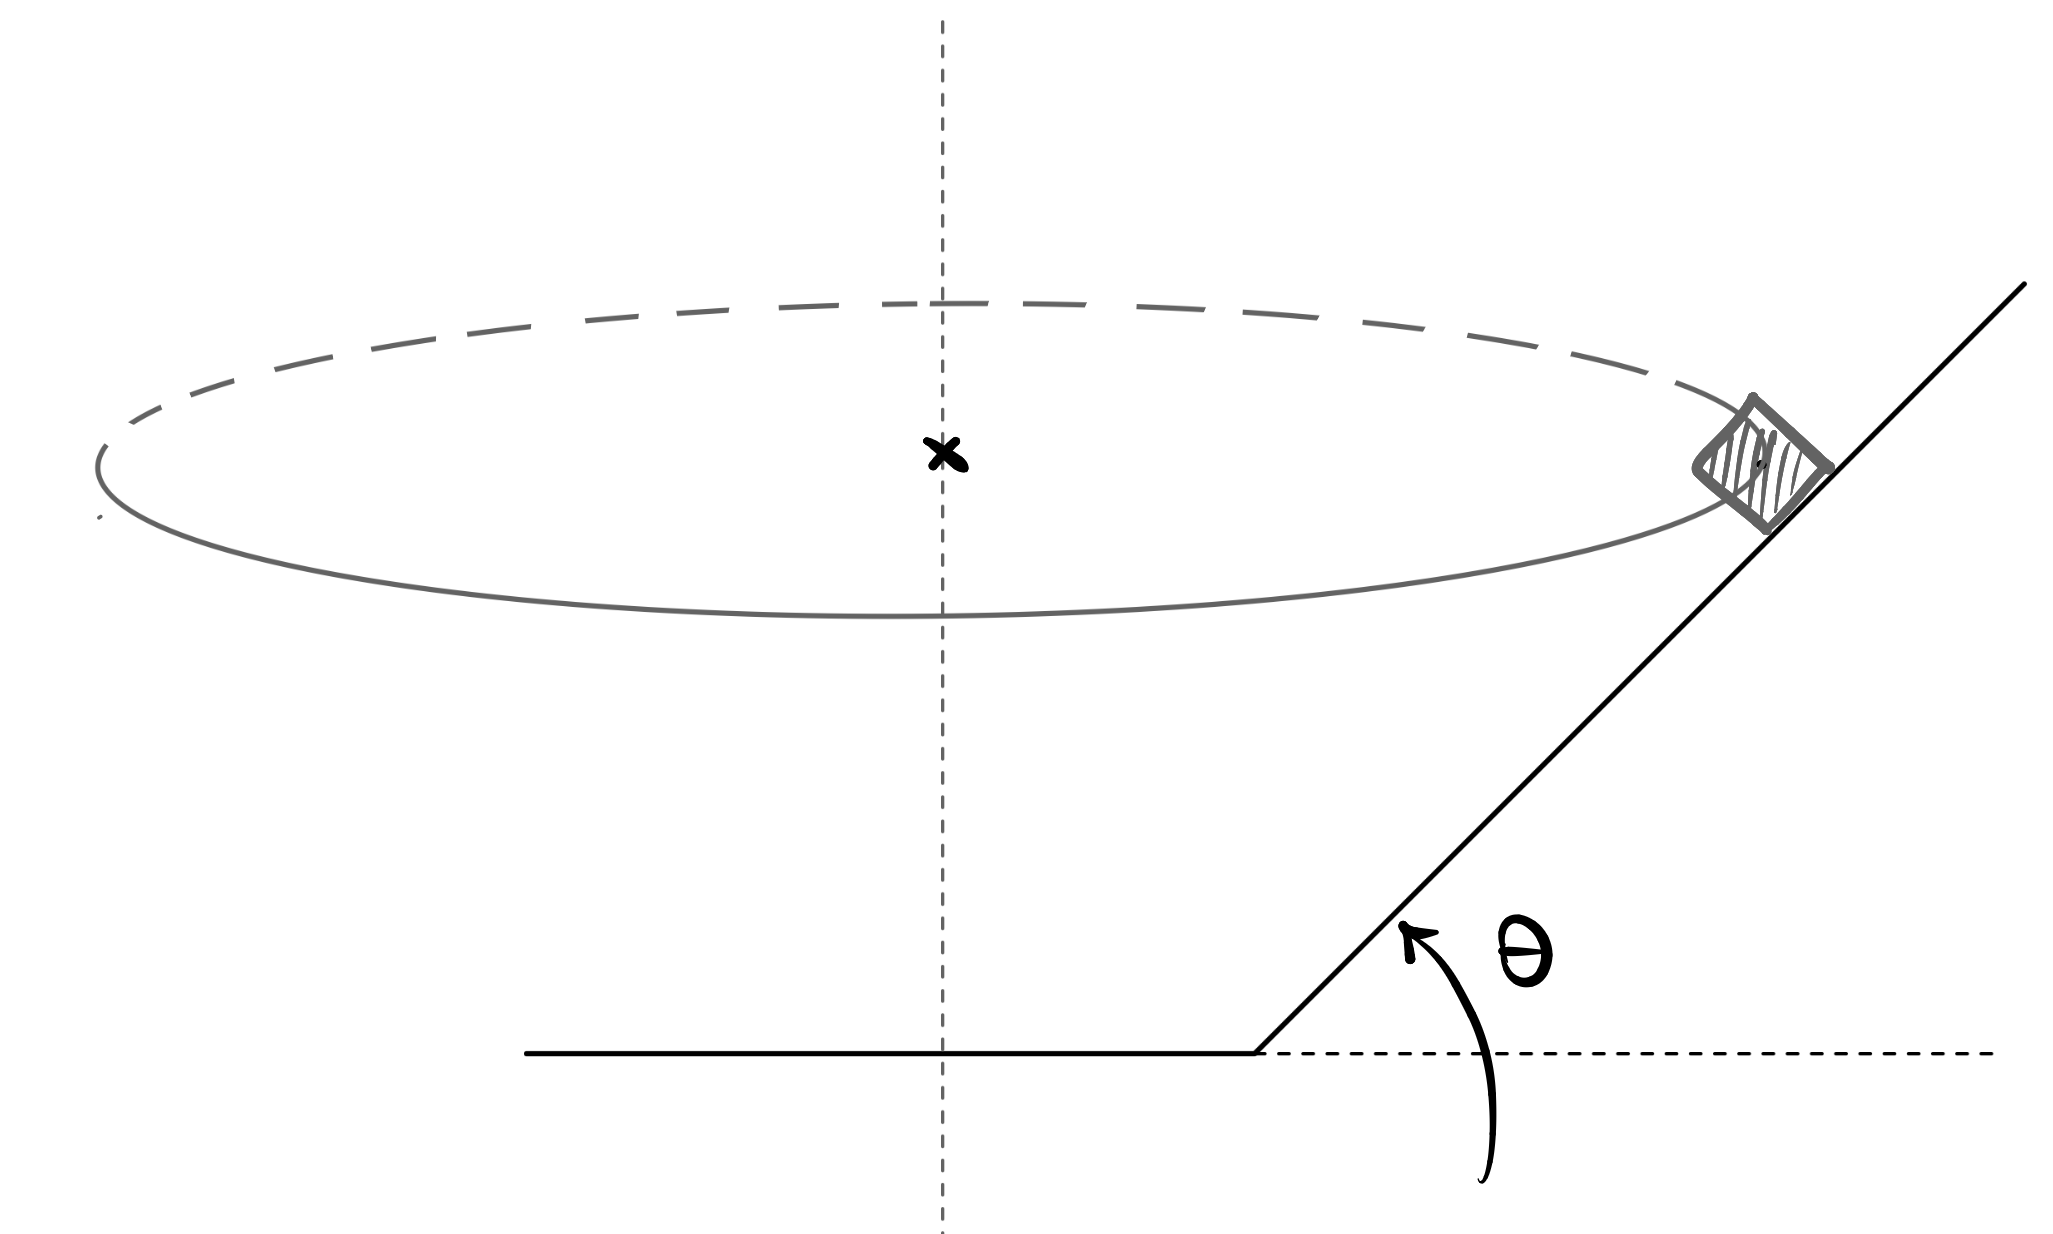
\includegraphics[width=0.35\linewidth]{imagensdinamicanewton/fcptcurva2.png}};
  \end{scope}
\end{tikzpicture}
\captionof{figure}{}
\label{fig_mec_fcptcurva02}
} 
\vspace{0.3cm}



Se o atrito entre o bloco e a pista é desprezível, qual é a velocidade que o bloco deve ter para conseguir descrever a circunferência de raio $R?$ 

\resolucao

Este não é exatamente o problema que originou a Equação \eqref{eq_newton_velocidademinimaparacurva}. Perceba que, neste caso, existem duas diferenças em relação àquele contexto: o solo não é horizontal e, além disso, lá havia atrito, e aqui o atrito é desprezível.

\medskip

A Figura \ref{fig_mec_fcptcurva03} mostra o diagrama das forças que atuam no bloco: o peso e a normal. Como sabemos, é preciso haver uma resultante de forças apontando para o centro da trajetória circular da caixa, de modo que o eixo centrípeto será horizontal. Assim, decomporemos as forças nos eixos vertical e horizontal, de modo que o peso ficará como está e quem será decomposta será a força normal, como mostra a segunda imagem da figura.

\vspace{0.3cm}
 {
\centering
\begin{tikzpicture}
  \begin{scope}[blend mode=multiply]
    \node {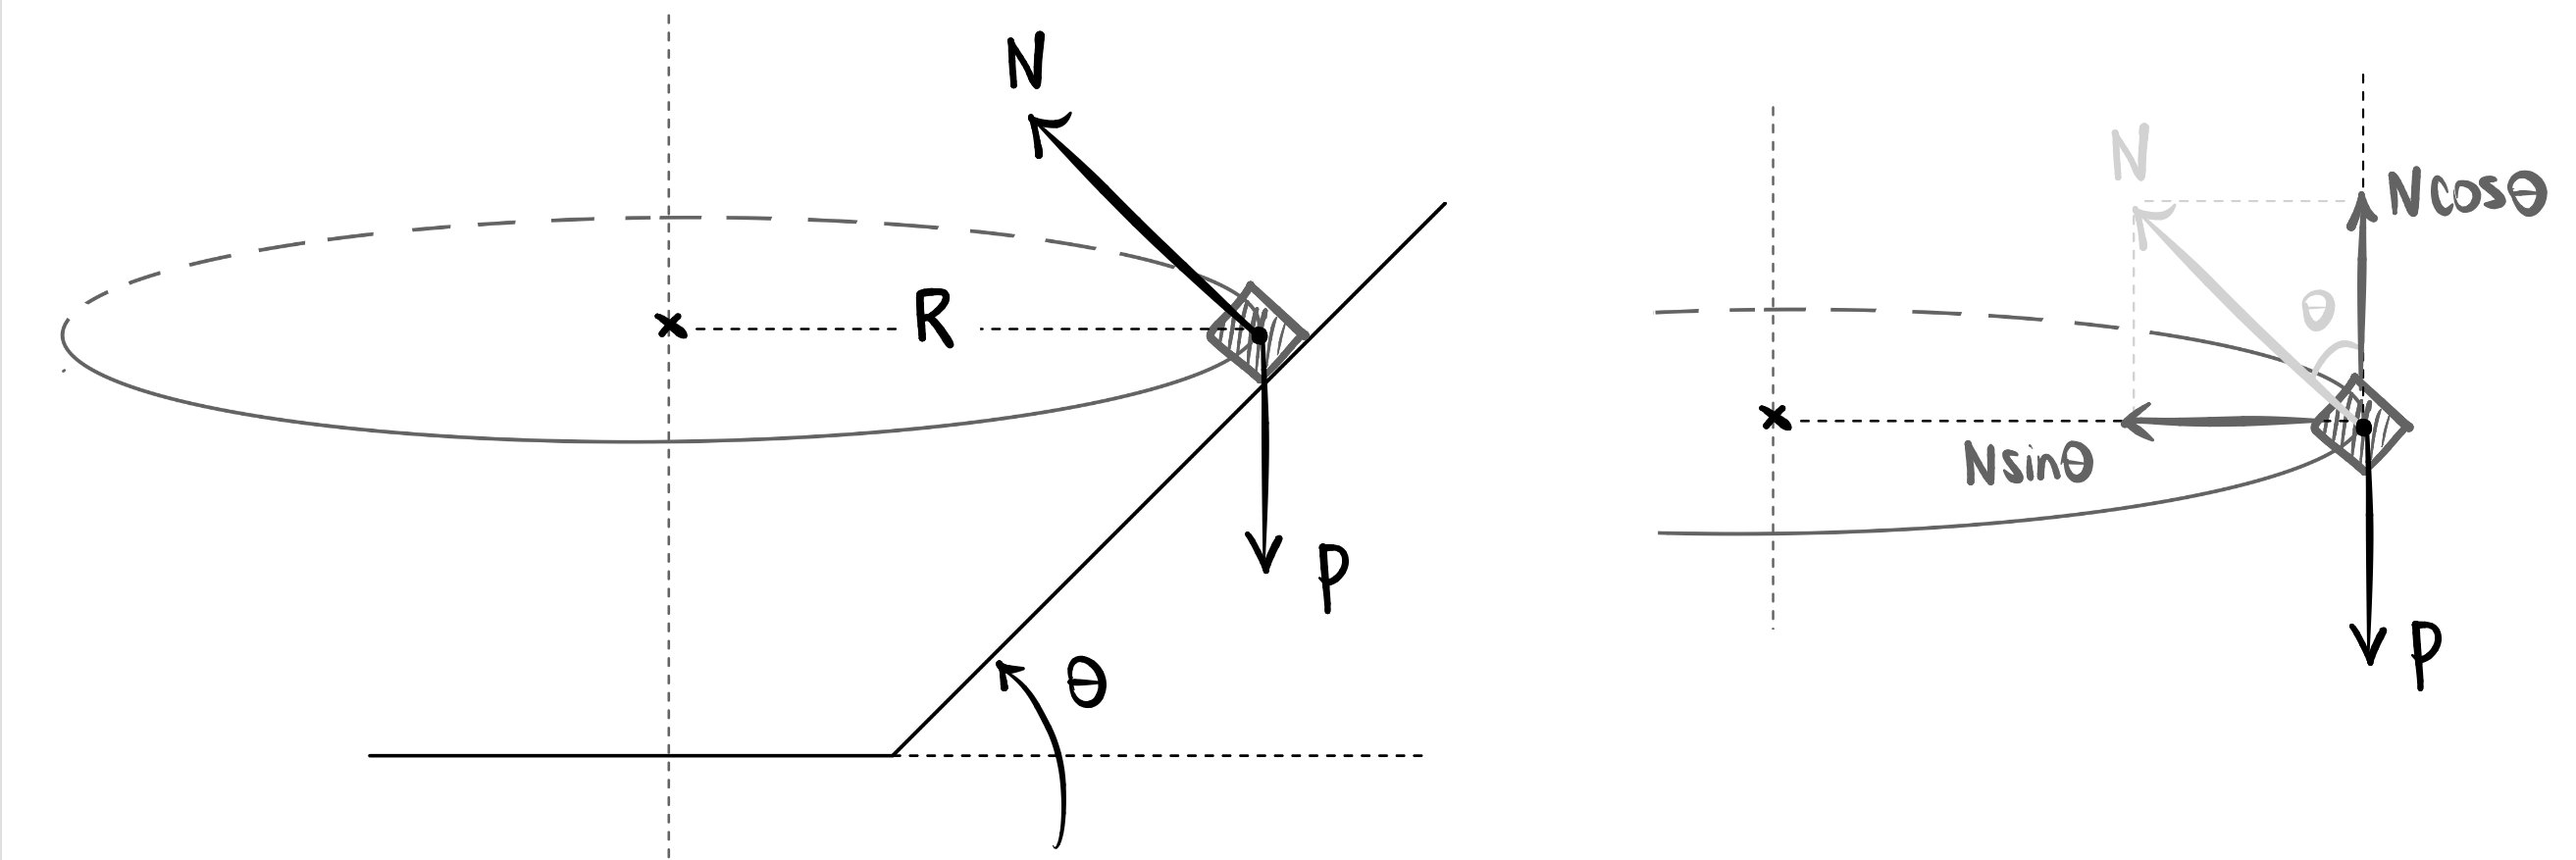
\includegraphics[width=0.8\linewidth]{imagensdinamicanewton/fcptcurva3.png}};
  \end{scope}
\end{tikzpicture}
\captionof{figure}{}
\label{fig_mec_fcptcurva03}
} 
\vspace{0.3cm}

Na vertical há equilíbrio, uma vez que a trajetória circular fica sempre no mesmo plano horizontal:

$$ F_{\text{R}_{\text{y}}} = 0 \implies N \cos \theta = P=mg.$$

Já na direção radial temos a componente horizontal da normal atuando como resultante centrípeta:

$$ F_{\text{R}_{\text{CPT}}} = N \sin \theta = \dfrac{mv^2}{R}.$$

Dividindo, membro a membro, as duas equações acima, teremos

$$ \dfrac{\cancel N \sin \theta}{\cancel N \cos \theta} = \dfrac{\dfrac{\cancel mv^2}{R}}{\cancel mg} \implies v^2 = Rg \tan \theta \implies \boxed{v=\sqrt{Rg \tan \theta}.}$$

Tal relação é o análogo da Equação \eqref{eq_newton_velocidademinimaparacurva}, porém para o caso em que o atrito é desprezível. Ou seja, mesmo sem atrito, é possível com que o objeto execute uma curva. Isso só ocorre por conta da inclinação do solo, que faz surgir uma componente horizontal da normal que é quem faz papel de resultante centrípeta. Perceba que, para um solo horizontal, isto é, para $\theta = 0,$ a equação acima diz que a velocidade da caixa é nula:

$$ \theta = 0 \implies \tan \theta = 0 \implies \boxed{v =0.}$$

Ou seja, em um solo horizontal -- que é a situação do desenvolvimento da Equação \eqref{eq_newton_velocidademinimaparacurva} -- é impossível fazer curva sem atrito.



\end{exemplo}


\vspace{0.3cm}


\begin{exemplo}[Nível III]\label{exemplo_newton_velocidademinimacurvahorizontalex03}

Considere a mesma situação do exemplo anterior, porém agora existe atrito entre o bloco e o plano, sendo o coeficiente de atrito estático igual a $\mu_e.$

Qual é o intervalo de possíveis valores de velocidade do bloco para que ele esteja descrevendo a circunferência de raio $R$ sem escorregar em relação ao plano?

\resolucao

A análise é semelhante àquela do exemplo anterior, com o único detalhe de que agora temos uma força a mais a considerar: a força de atrito. Neste caso, há duas situações a se considerar: aquela em que a velocidade é a menor possível para que a caixa não escorregue e aquela em que a velocidade é a maior possível. 

\medskip

Consideremos a primeira situação, representada na Figura \ref{fig_mec_fatefcptvmin}. Note que, se a caixa tem a menor velocidade possível, sua tendência é escorregar plano abaixo (considere a situação limite em que $v=0$: a caixa tende a escorregar ao longo do plano para baixo). Neste caso, o atrito, contrariando a tendência de movimento, irá atuar na direção do plano, porém para cima.

\vspace{0.3cm}
 {
\centering
\begin{tikzpicture}
  \begin{scope}[blend mode=multiply]
    \node {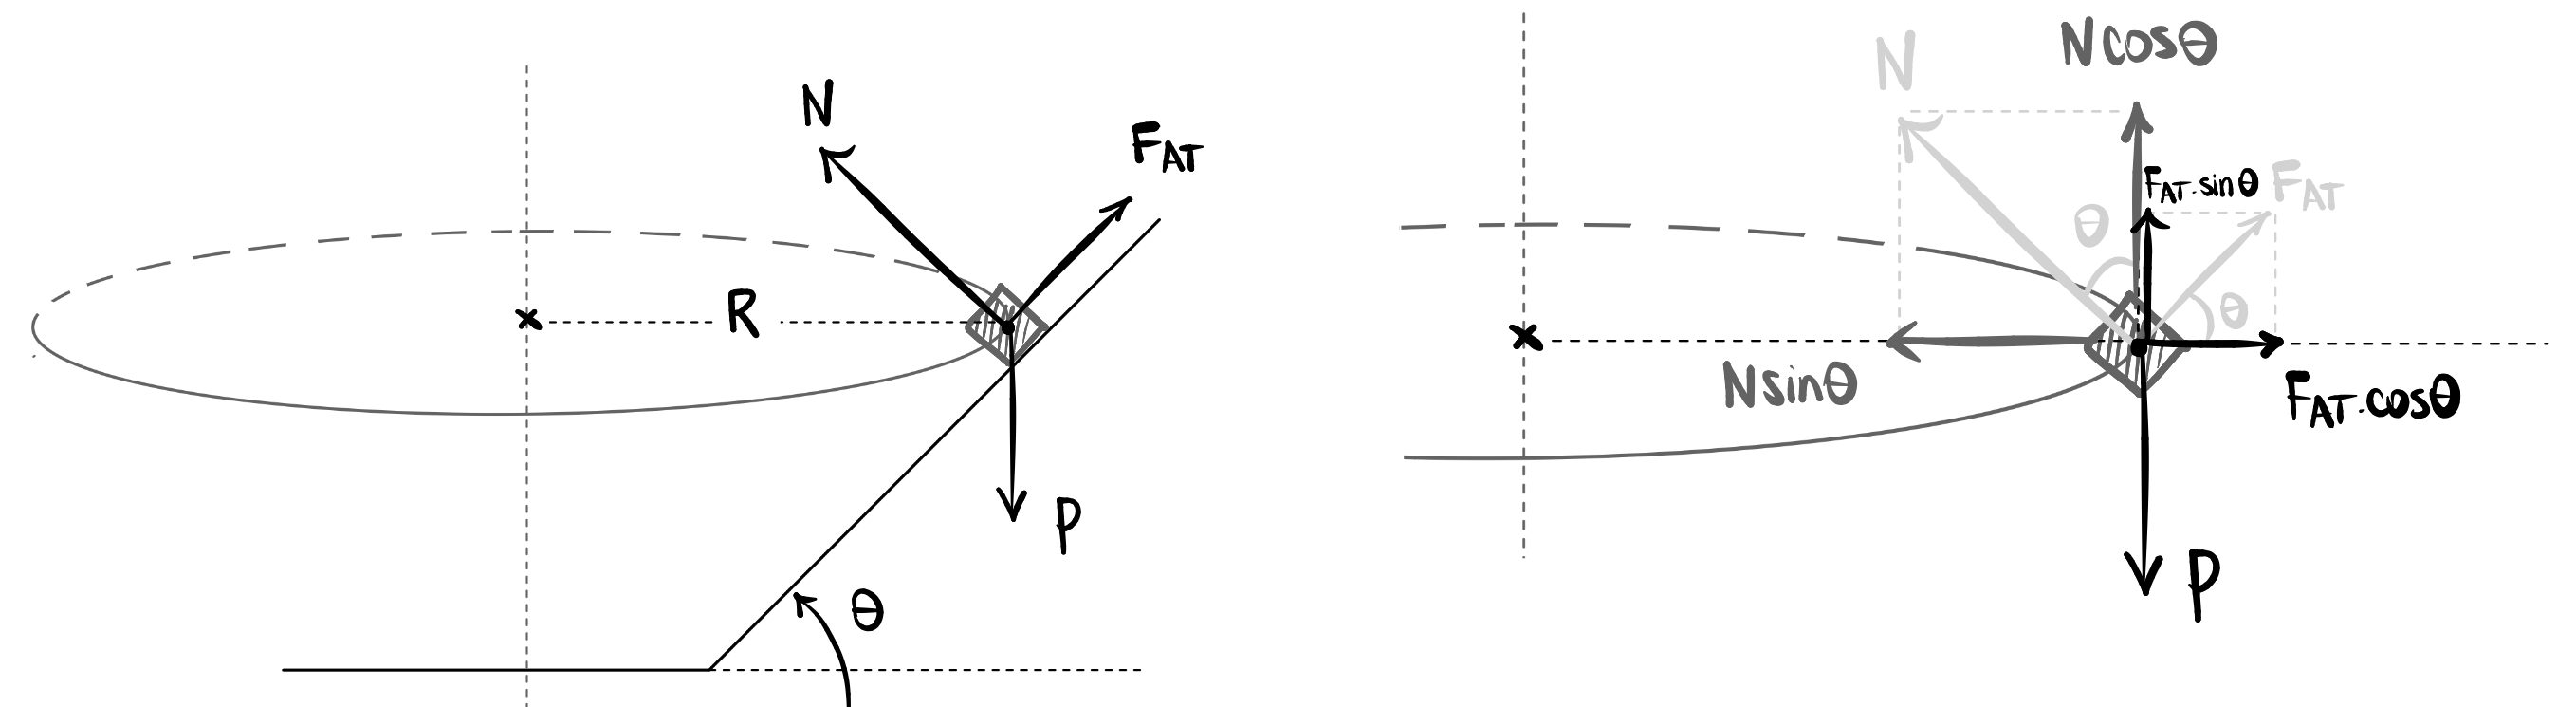
\includegraphics[width=0.9\linewidth]{imagensdinamicanewton/fatefcptvmin.png}};
  \end{scope}
\end{tikzpicture}
\captionof{figure}{Situação de velocidade mínima.}
\label{fig_mec_fatefcptvmin}
} 
\vspace{0.3cm}

A segunda imagem da figura já mostra as forças decompostas, e o equacionamento seguirá o mesmo princípio daquele  do exemplo anterior. Ou seja, na vertical há equilíbrio, uma vez que a trajetória circular fica sempre no mesmo plano horizontal:

$$ F_{\text{R}_{\text{y}}} = 0 \implies N \cos \theta + F_{\text{AT}} \sin \theta =mg.$$

Já na direção radial teremos:

$$ F_{\text{R}_{\text{CPT}}} = N \sin \theta - F_{\text{AT}} \cos \theta = \dfrac{mv^2}{R}.$$

Considerando que estamos na situação limite -- isto é, o atrito é o estático máximo -- teremos que $F_{\text{AT}}=\mu_e N$, o que, nas equações acima, fornece

$$
\begin{cases}
N \cos \theta + \mu_e N \sin \theta  = mg \\

N \sin \theta - \mu_e N \cos \theta = \dfrac{mv^2}{R},

\end{cases}
$$

\noindent e, dividindo as equações acima membro a membro, teremos

$$ \dfrac{\cancel N \left( \sin \theta - \mu_e \cos \theta\right)}{\cancel N \left( \cos \theta + \mu_e \sin \theta \right) } = \dfrac{\dfrac{\cancel mv^2}{R}}{\cancel mg},$$
\

\noindent e, dividindo o numerador e o denominador por $\cos\theta$ do lado esquerdo, teremos

$$ \boxed{ v_{\text{min}} = \sqrt{Rg} \sqrt{ \left( \dfrac{\tan \theta - \mu_e}{1 + \mu_e \tan \theta}\right)}.} $$

Ou seja, na situação em que a tendência do bloco é de escorregar plano abaixo -- e, portanto, ele teria a menor velocidade possível para estar em tal movimento -- essa será a sua velocidade. 

\medskip

Já na situação de velocidade máxima a tendência do bloco é subir plano acima (ser lançado para fora da pista), de modo que o atrito, contrariando a tendência de movimento, atua na direção do plano, porém para baixo. A Figura \ref{fig_mec_fatefcptvmax} ilustra essa situação. A única diferença aqui, portanto, é o sentido da força de atrito, que fica invertido.

\vspace{0.3cm}
 {
\centering
\begin{tikzpicture}
  \begin{scope}[blend mode=multiply]
    \node {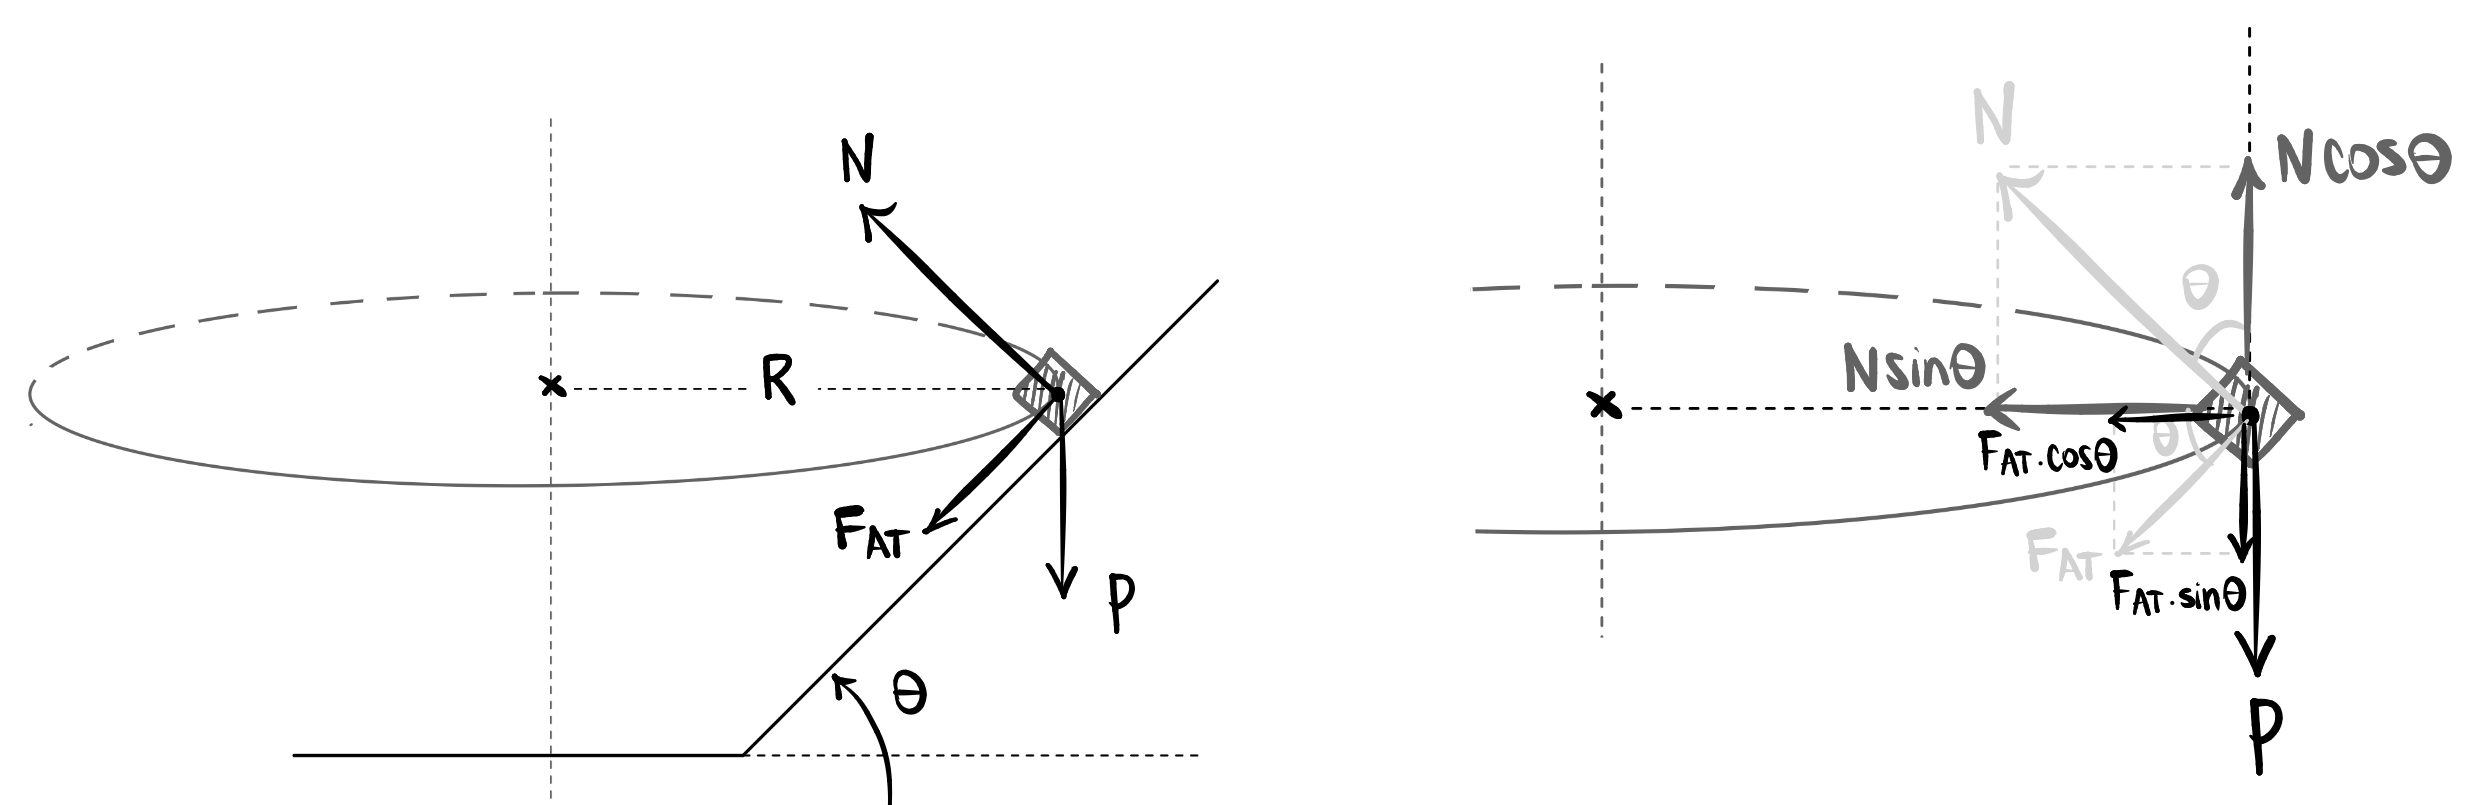
\includegraphics[width=0.9\linewidth]{imagensdinamicanewton/fatefcptvmax.png}};
  \end{scope}
\end{tikzpicture}
\captionof{figure}{Situação de velocidade máxima.}
\label{fig_mec_fatefcptvmax}
} 
\vspace{0.3cm}

Aplicando, portanto, o mesmo raciocínio do  caso anterior, isto é, escrevendo que

$$ \begin{cases}
    F_{\text{R}_{\text{y}}} = 0 \\
    F_{\text{R}_{\text{CPT}}} =\dfrac{mv^2}{R},
\end{cases}$$

\noindent somos levados a

$$ \boxed{ v_{\text{max}} = \sqrt{Rg} \sqrt{ \left( \dfrac{\tan \theta + \mu_e}{1 - \mu_e \tan \theta}\right)}.} $$

Assim, a velocidade $v$ da caixa para que ela execute a rotação sem escorregar em relação ao plano é tal que

$$ \sqrt{Rg} \sqrt{ \left( \dfrac{\tan \theta - \mu_e}{1 + \mu_e \tan \theta}\right)} \leq v \leq \sqrt{Rg} \sqrt{ \left( \dfrac{\tan \theta + \mu_e}{1 - \mu_e \tan \theta}\right)}. $$


\end{exemplo}





\newpage

\section{Impulso e Momento Linear}


A partir de agora vamos começar a trabalhar com algumas grandezas e equações que constituem, em última instância, apenas uma forma de se reescrever as leis de Newton. 

Essas novas grandezas -- impulso e momento linear -- substituirão as forças e a velocidade, possibilitando reescrever a Segunda Lei de Newton em termos dessas novas grandezas, o que é feito no chamado Teorema do Impulso, expresso na Equação \eqref{eq_newton_teoremaimpulso}.

O que será feito nessa seção, portanto, não constitui exatamente um conteúdo novo: trata-se apenas das próprias leis de Newton reescritas em termos de uma nova linguagem. Tentaremos deixar isso sempre claro ao longo do desenvolvimento de cada equação a fim de que o leitor tenha clareza de como essas duas linguagens se relacionam. 







\begin{secnivel}[Momento Linear]{I}{Momento Linear}
  
  \eqLdois{def}{eq_newton_momentolinear}{\vec p := m \vec v.}

\end{secnivel}






\secgfe{De onde vem}

O momento linear $\vec p$ de uma partícula (ou quantidade de movimento, representado por $\vec Q$ em algumas literaturas) é definido como sendo o produto da massa $m$ da partícula pela sua velocidade $\vec v.$

Note, de imediato, que o momento linear é uma grandeza vetorial: ele é o produto do vetor velocidade $\vec v$ por um escalar\footnote{Lembre-se: um escalar é apenas um número real. É uma grandeza que não possui direção e sentido, apenas valor numérico (módulo).} (a massa $m,$ no caso). Sendo tal escalar sempre positivo, o momento linear $\vec p$ de uma partícula é um vetor que aponta na mesma direção e sentido do vetor velocidade dessa partícula, como mostra a Figura \ref{fig_newton_momentolinear01}. Em tal figura peço ao leitor a gentileza de não confundir o momento linear $\vec p$ com o peso $\vec P$ da partícula. Tratam-se de duas grandezas que não possuem relação alguma, exceto por guardarem a coincidência de serem representadas pela mesma letra.



\vspace{0.3cm}
{
\centering
\begin{tikzpicture}
  \begin{scope}[blend mode=multiply]
    \node {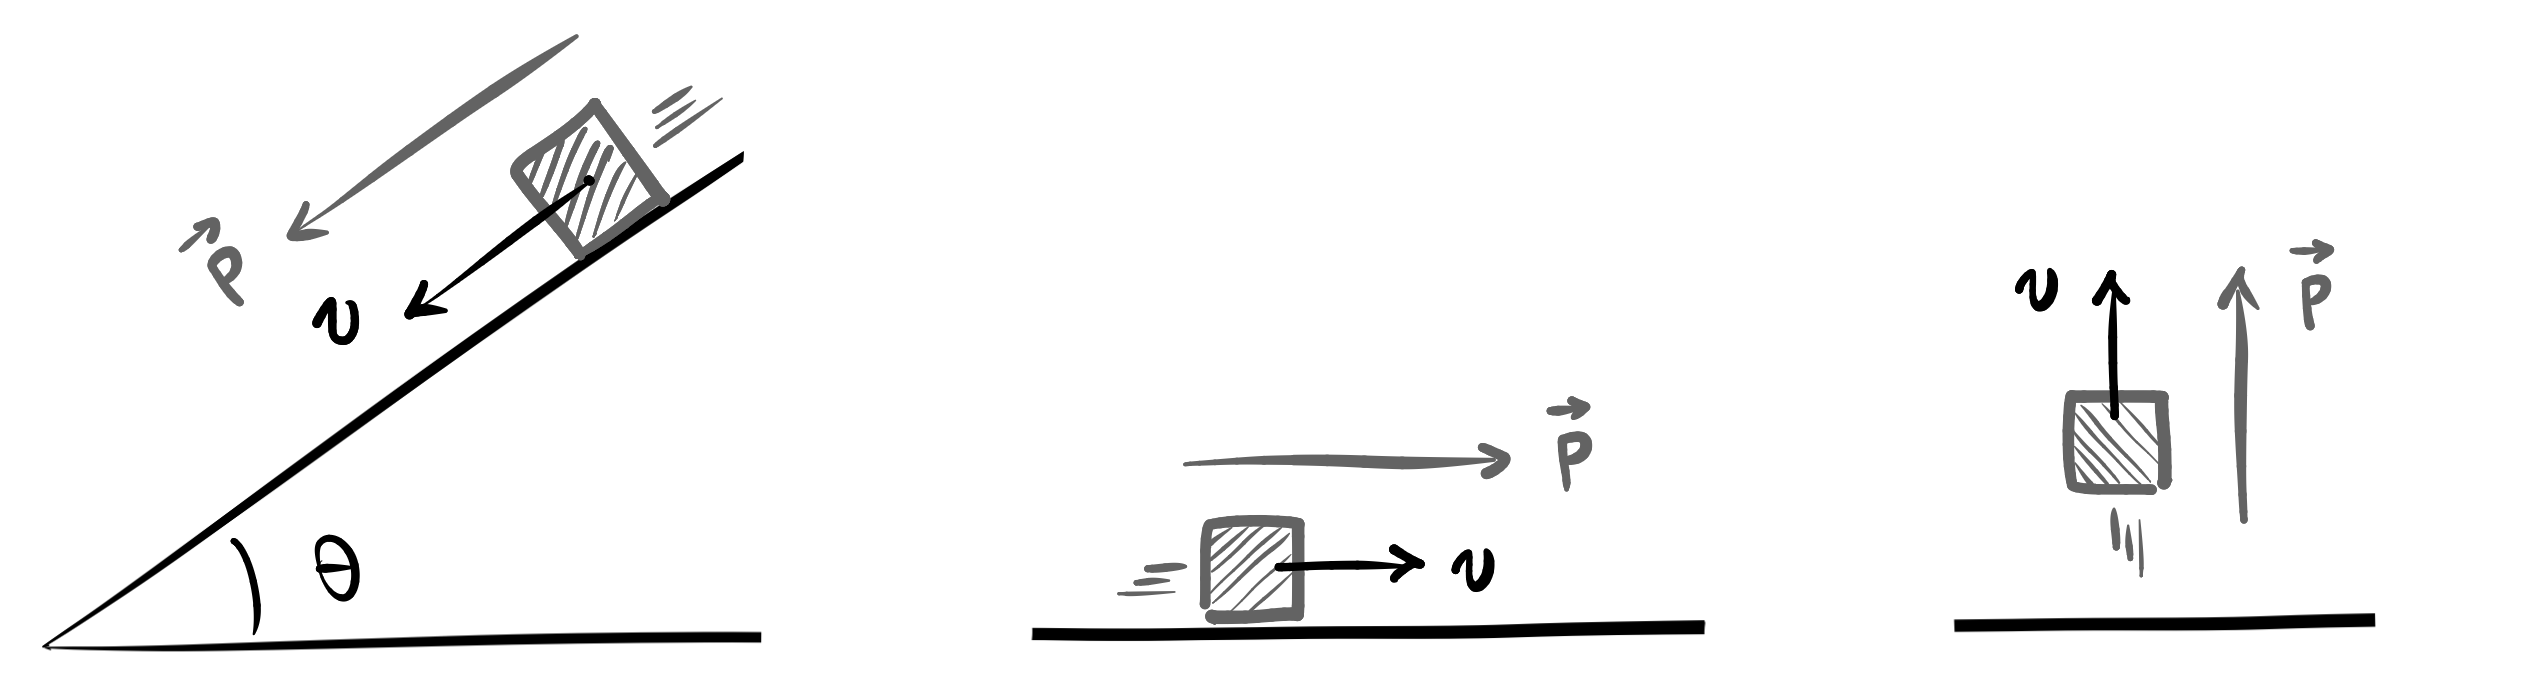
\includegraphics[width=0.8\linewidth]{imagensdinamicanewton/momentolinear01.png}};
  \end{scope}
\end{tikzpicture}
\captionof{figure}{O momento linear $\vec p$ é sempre paralelo e aponta no mesmo sentido da velocidade $\vec v$ da partícula.}
\label{fig_newton_momentolinear01}
} 
\vspace{0.3cm}

Perceba, portanto, que a quantidade de movimento de um corpo só será constante em dois casos: caso ele esteja em repouso ou em MRU. Estas são as únicas situações, como vimos no desenvolvimento da Equação \eqref{eq_dinamica1_segundaleinewton}, em que o vetor velocidade é constante: ele não muda em módulo, direção nem em sentido. Em qualquer movimento que faça curva, como o vetor $\vec v$ varia -- ao menos em direção --, o momento linear $\vec p$ também irá variar. A essa altura o leitor poderia se perguntar

\begin{center}
    \textit{Qual é a razão de se criar uma nova grandeza para descrever o movimento de um corpo, se já temos a velocidade?}
\end{center}

Para respondê-la, observe a situação da Figura \ref{fig_newton_momentolinear05}, que mostra um carro e um ônibus que estão prestes a colidir contra uma parede de concreto. Considere que a massa do carro é de 600kg e a do ônibus é de 6.000kg. Em qual dos dois casos a parede de concreto precisará realizar mais força a fim de parar o veículo?

\vspace{0.3cm}
{
\centering
\begin{tikzpicture}
  \begin{scope}[blend mode=multiply]
    \node {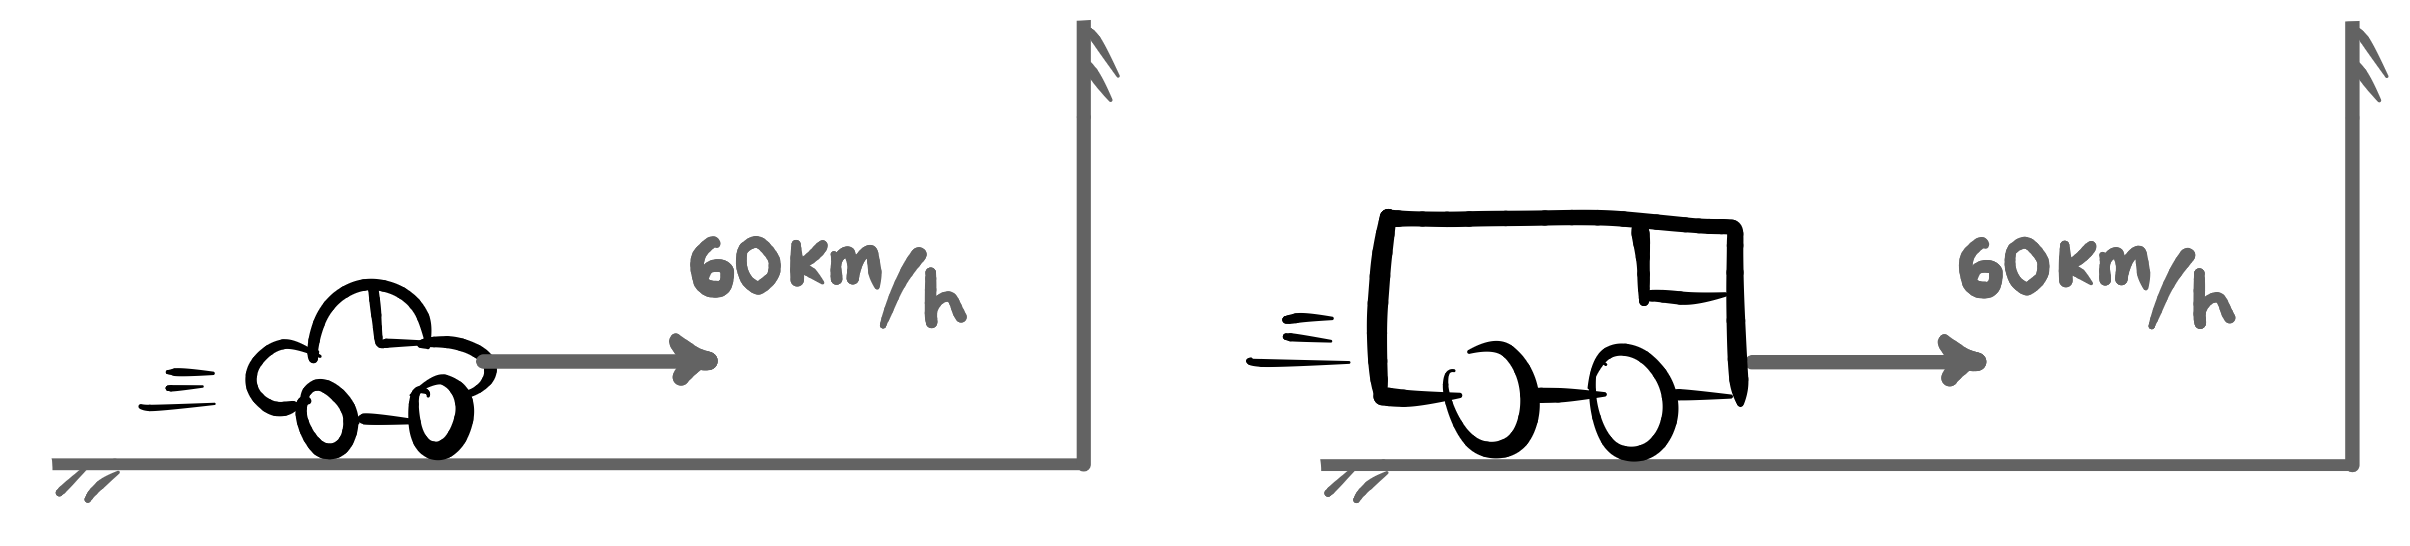
\includegraphics[width=0.7\linewidth]{imagensdinamicanewton/momentolinear05.png}};
  \end{scope}
\end{tikzpicture}
\captionof{figure}{O momento linear $\vec p$ carrega uma informação a mais que a velocidade $\vec v:$ a inércia do corpo.}
\label{fig_newton_momentolinear05}
} 
\vspace{0.3cm}

Note que os dois possuem a mesma velocidade, mas certamente o leitor haverá de concordar -- apenas por intuição, por ora -- que, a fim de parar o ônibus, a parede deverá exercer mais força, ainda que este se mova com a mesma velocidade que o carro.

Ora, veja, portanto, que o conceito de velocidade não captura completamente toda a informação a respeito do movimento de um corpo. Isso ocorre porque dois objetos que possuem a mesma velocidade -- como o carro e o ônibus -- podem possuir inércias diferentes. Como sabemos, a inércia é o que medirá o quão fácil ou difícil será alterar o estado de movimento daquele corpo e, como vimos no desenvolvimento da Equação \eqref{eq_dinamica1_segundaleinewton}, a inércia é medida pela massa de um corpo.

A ideia aqui é que nem a velocidade nem a massa, isoladamente, são suficientes para descrever o “estado de movimento” de um corpo. Um caminhão muito massivo se deslocando lentamente pode ser muito mais difícil de parar do que uma bola de tênis em alta velocidade — mas, ao mesmo tempo, uma bala extremamente rápida também oferece enorme resistência à mudança de movimento. Há, portanto, algo mais profundo acontecendo: uma combinação entre “quão pesado” é o corpo e “quão rápido” ele se move.


Desse modo, ao definir o momento linear (ou quantidade de movimento) de um corpo por meio do produto da massa pela velocidade, conseguimos construir uma grandeza que mensure essas duas características em uma única medida. O momento linear, portanto, constitui uma nova grandeza física que consegue, de forma simples, quantificar o movimento levando em conta tanto a inércia (massa) quanto a velocidade. E é por isso que é mais difícil parar o ônibus da Figura \ref{fig_newton_momentolinear05} do que o carro: apesar de terem a mesma velocidade, o ônibus possui maior \textit{quantidade de movimento} (momento linear) e, como veremos, a força necessária para parar um objeto estará relacionada ao quão rápido o momento linear varia, e não com a velocidade isoladamente. Isso é evidenciado pela Equação \eqref{eq_newton_teoremaimpulso}.\footnote{Caso o leitor tenha se indagado a respeito do dano causado à parede ou aos veículos nas colisões da situação da Figura \ref{fig_newton_momentolinear05}, cabe destacar que isso estará relacionado à energia cinética dos corpos, grandeza que definiremos mais adiante em nosso estudo.}




\secgfe{Onde é usada}

Como veremos mais adiante, o conceito de momento linear e impulso serão bastante utilizados em problemas que envolvam colisões. Isso ficará mais claro no desenvolvimento da Equação \eqref{eq_newton_convervacaomomentolinear}.



\secgfe{Erros comuns}

O erro mais comum aqui certamente é o de ignorar o caráter vetorial do momento linear. Considere, por exemplo, o problema se calcular a variação do momento linear da bolinha de massa $m=3$ kg representada na Figura \ref{fig_newton_momentolinear02}. Tal bolinha se aproxima de uma parede a uma velocidade de $5$ m/s, colidindo contra a parede e invertendo o sentido do seu movimento, porém mantendo o mesmo valor de velocidade.

O leitor mais ingênuo computaria que, antes da colisão, o momento da partícula é 
$$p_0=mv_0 = 3 \cdot 5 = 15 \text{kg} \cdot \text{m/s}. $$
Após a colisão, o momento final da partícula seria 
$$p_f=mv_f = 3 \cdot 5 = 15 \text{kg} \cdot \text{m/s},$$

\noindent de modo que a variação do momento foi nula:


$$ \Delta p = p_f - p_0 = 15 - 15 = 0.$$

Tal raciocínio (e consequentemente o resultado) está, contudo, errado.

\vspace{0.3cm}
{
\centering
\begin{tikzpicture}
  \begin{scope}[blend mode=multiply]
    \node {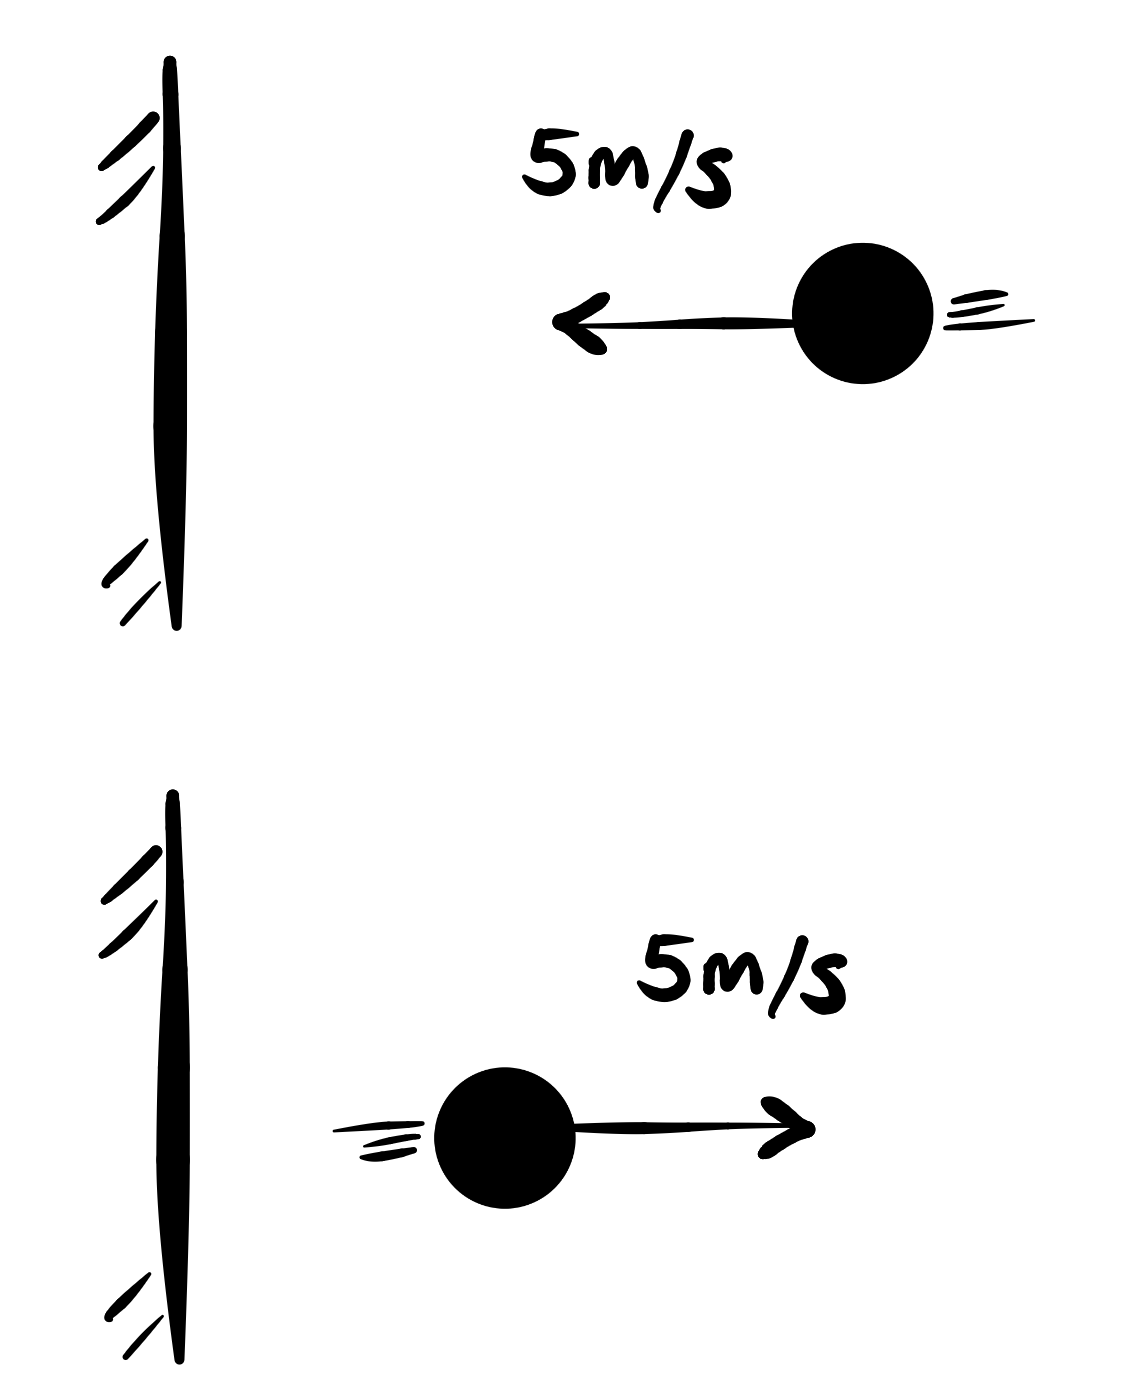
\includegraphics[width=0.25\linewidth]{imagensdinamicanewton/momentolinear02.png}};
  \end{scope}
\end{tikzpicture}
\captionof{figure}{O momento linear é uma grandeza vetorial.}
\label{fig_newton_momentolinear02}
} 
\vspace{0.3cm}

Isso porque, sendo o momento linear uma grandeza vetorial, ele herda todas as características vetoriais do vetor velocidade $v.$ Sendo assim, temos que atribuir sinais distintos a velocidades em sentidos opostos, uma vez que trata-se de uma grandeza vetorial. Logo, adotando o sentido positivo como sendo para a direita, a velocidade inicial é, na verdade, $v_0=-5$ m/s, de modo que o momento inicial é 
$$p_0=mv_0 = 3 \cdot (-5) = -15 \text{kg} \cdot \text{m/s}. $$
A velocidade final, apontando para a direita (sentido adotado como positivo) é $v_f=+5$ m/s, de modo que o momento final é 
$$p_f=mv_f = 3 \cdot 5 = 15 \text{kg} \cdot \text{m/s},$$

\noindent e a variação do momento é, portanto


$$ \Delta p = p_f - p_0 = 15 - (-15) = 30 \text{kg} \cdot \text{m/s}.$$

Caso o leitor prefira interpretar de forma puramente vetorial tal resultado, note que o vetor $\vec p_0$ tem módulo igual a $15 \text{kg} \cdot \text{m/s}$ e aponta para a esquerda, enquanto que o vetor $\vec p_f$ tem módulo igual a $15 \text{kg} \cdot \text{m/s}$ e aponta para a direita, como mostra a Figura \ref{fig_newton_momentolinear03}. Assim, o vetor $-\vec p_0$ aponta no sentido oposto de $\vec p_0,$ ou seja, para a direita. 

Logo, como o que queremos computar é 

$$ \Delta \vec p = \vec p_f - \vec p_0,$$

\noindent teremos os dois vetores ($\vec p_f$ e $-\vec p_0)$ na mesma direção e sentido, de modo que o vetor resultante $ \Delta \vec p = \vec p_f +(- \vec p_0)$ terá módulo igual a $15+15 =30 \text{kg} \cdot \text{m/s}. $

\vspace{0.3cm}
{
\centering
\begin{tikzpicture}
  \begin{scope}[blend mode=multiply]
    \node {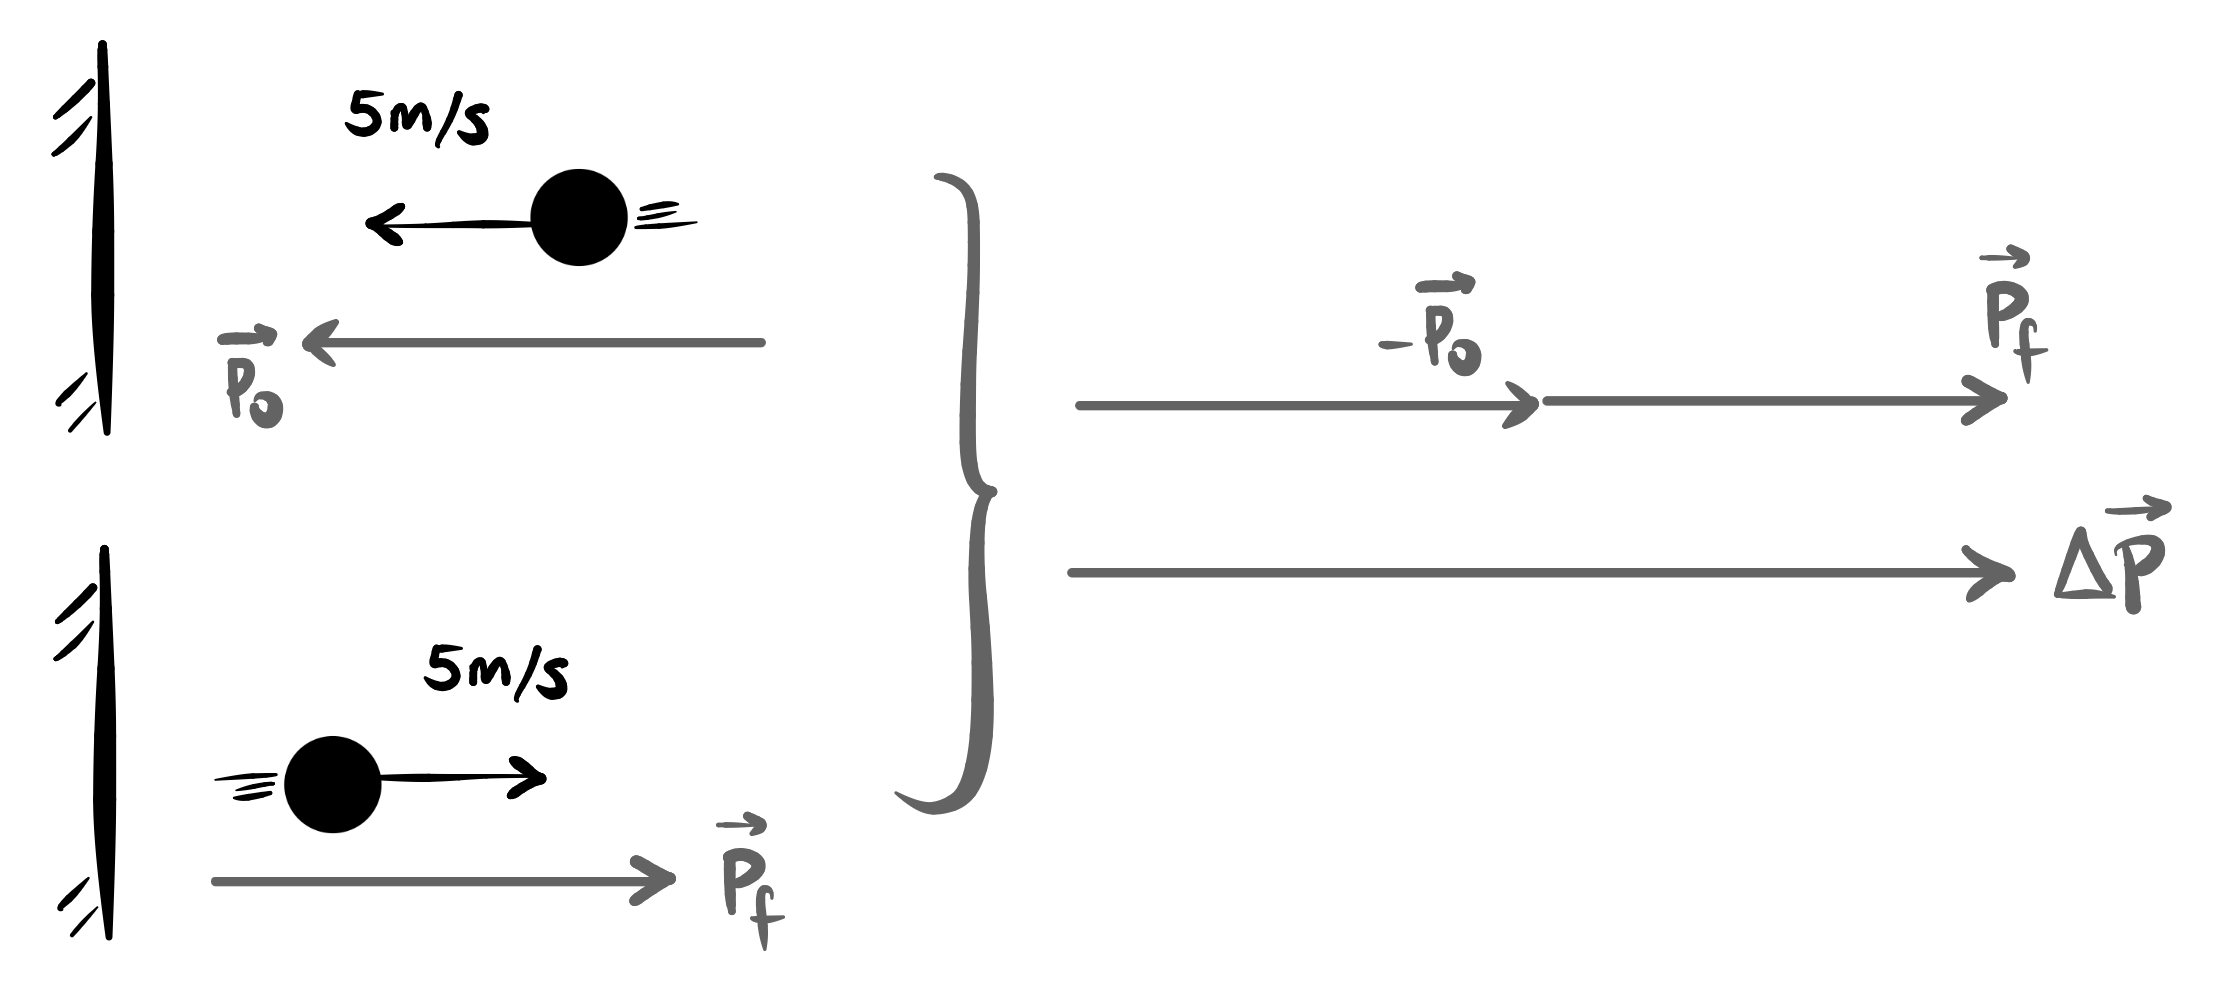
\includegraphics[width=0.65\linewidth]{imagensdinamicanewton/momentolinear03.png}};
  \end{scope}
\end{tikzpicture}
\captionof{figure}{A variação do momento linear interpretada de forma vetorial.}
\label{fig_newton_momentolinear03}
} 
\vspace{0.3cm}


\secgfe{Observações}

A unidade de medida no S.I. de velocidade é o m/s, enquanto a unidade de medida de massa é o kg. Assim, a unidade de medida padrão para momento linear é

$$ [p] = [m] \cdot [v] = \text{kg} \cdot \text{m/s},$$

\noindent que é lido exatamente dessa forma, sem receber um nome especial: quilograma metro por segundo.


Um corpo de massa $m=10$ kg se movendo a uma velocidade $v=2$ m/s possui, portanto, um momento linear 

$$ p = mv = 10 \text{kg} \cdot 2 \text{m/s} = 20 \text{kg} \cdot \text{m/s},$$

\noindent que é lido como vinte quilogramas metro por segundo.


\vspace{0.3cm}


\begin{exemplo}[Nível I]\label{exemplo_newton_momentumex01}

Dois carros trafegam na mesma direção e sentido. O carro A tem massa
$1200\,\text{kg}$ e velocidade $20\,\text{m/s}$; o carro B tem massa
$400\,\text{kg}$ e velocidade $80\,\text{m/s}$. Qual tem o maior momento linear?

\resolucao

Os momentos lineares de cada carro são:

$$p_A = 1200\cdot 20 = 24\,000\,\text{kg·m/s}, \qquad
  p_B = 400\cdot 80 = 32\,000\,\text{kg·m/s}.$$

O carro B tem maior momento linear. O carro mais leve tem mais momento: a
velocidade quatro vezes maior mais que compensa a massa três vezes menor.
O momento linear não é determinado pela massa isoladamente, nem pela
velocidade isoladamente --- mas pelo produto de ambas.

\end{exemplo}


\vspace{0.3cm}




\begin{exemplo}[Nível II]\label{exemplo_newton_momentumex02}

Ronaldinho Gaúcho -- o bruxo -- bate uma falta em um importante jogo de futebol, chutando a bola com velocidade inicial de $40$ m/s. Se a massa da bola é de 500g e ela bate no travessão, saindo em uma direção perpendicular a da direção inicial de movimento, com uma velocidade de $30$ m/s, calcule o módulo da variação da momento linear da bola antes e depois de bater na trave.

\resolucao

O momento inicial da bola tem módulo igual a $p_0= 0.5 \text{kg} \cdot 40 \text{m/s}  = 20\text{kg} \cdot \text{m/s}$, enquanto que o momento final tem módulo dado por  $p_f= 0.5 \text{kg} \cdot 30 \text{m/s}  = 15\text{kg} \cdot \text{m/s}$.

A Figura \ref{fig_newton_momentolinear04} ilustra o aspecto vetorial do momento. O que queremos é

$$ \Delta \vec p = \vec p_f - \vec p_0 = \vec p = \vec p_f + (- \vec p_0), $$

\noindent de modo que vamos somar o vetor $\vec p_f$ com o vetor $(- \vec p_0)$, o que aparece ilustrado na parte direita da figura.

{
\centering
\begin{tikzpicture}
  \begin{scope}[blend mode=multiply]
    \node {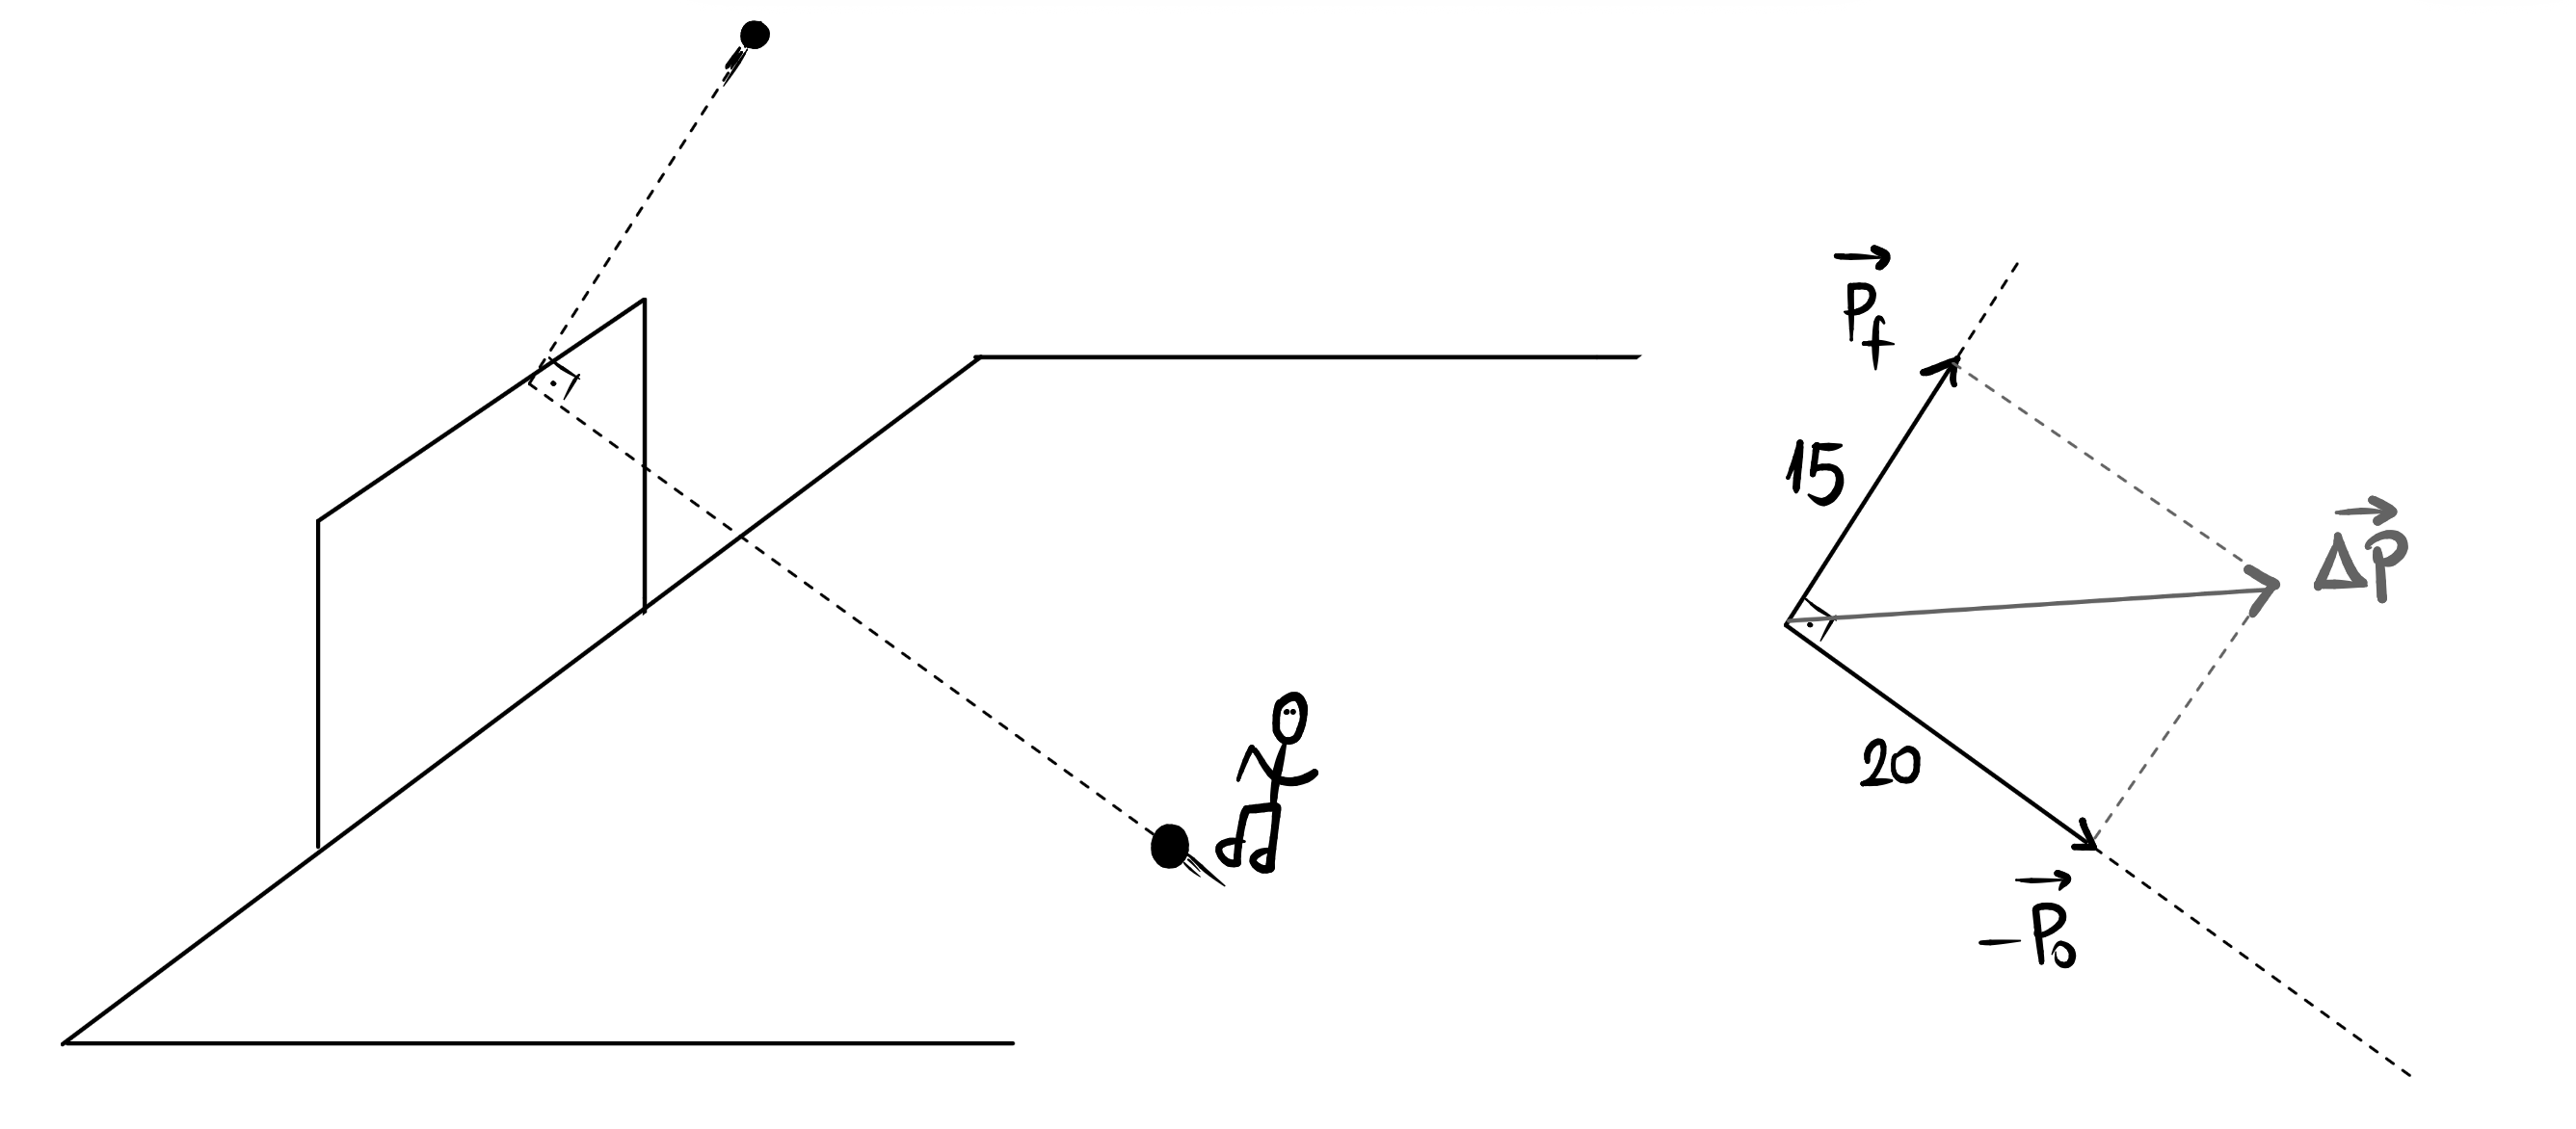
\includegraphics[width=0.8\linewidth]{imagensdinamicanewton/momentolinear04.png}};
  \end{scope}
\end{tikzpicture}
\captionof{figure}{A variação do momento linear em um caso bidimensional.}
\label{fig_newton_momentolinear04}
} 
\vspace{0.3cm}

Podemos obter o valor de $|\Delta \vec p|$ por meio do Teorema de Pitágoras no triângulo retângulo da figura:

$$ |\Delta \vec p |^2 = |\vec p_f |^2 + |- \vec p_0 |^2 = 15^2 + 20^2 = 625 \implies \boxed{|\Delta \vec p | = 25 \text{kg} \cdot \text{m/s}.} $$

\end{exemplo}

\vspace{0.3cm}




\begin{exemplo}[Nível III]\label{exemplo_newton_momentumex03}

Dois blocos de massas $m_1 = 2\,\text{kg}$ e $m_2 = 8\,\text{kg}$ estão
conectados por um fio ideal que passa por uma polia ideal presa no teto. O sistema é
liberado do repouso e percorre $d = 0{,}75\,\text{m}$. Determine:

\begin{enumerate}
     \item [a)] a velocidade do sistema;
     \item [b)] o momento linear de cada bloco;
     \item [c)] o momento linear total do sistema.
\end{enumerate}


\resolucao

A força resultante sobre o sistema é $(m_2 - m_1)g$, agindo sobre a massa total
$m_1+m_2$. A aceleração é

$$ a = \frac{(m_2-m_1)\,g}{m_1+m_2} = \frac{6\cdot10}{10} = 6\,\text{m/s}^2. $$

Após percorrer $d = 0{,}75\,\text{m}$ a partir do repouso:

$$ v^2 = 2ad = 2\cdot6\cdot0{,}75 = 9 \implies v = 3\,\text{m/s}. $$

Os momentos individuais têm o mesmo módulo mas sentidos opostos ---
$m_1$ sobe, $m_2$ desce:

$$ p_1 = 2\cdot 3= 6\,\text{kg·m/s}\ (\uparrow), \qquad
   p_2 = 8\cdot 3= 24\,\text{kg·m/s}\ (\downarrow). $$

O momento total do sistema é a soma vetorial:

$$ |\vec{p}_{\,\text{total}} |= p_2 - p_1 = 24 - 6 = \boxed{18\,\text{kg·m/s}\ (\downarrow).} $$

O momento total do sistema não é $(m_1+m_2)v$, mas $(m_2-m_1)v$. Como os
blocos se movem em sentidos opostos, seus momentos se subtraem vetorialmente. Somar os módulos seria ignorar que momento linear é uma grandeza vetorial.



\end{exemplo}

\vspace{0.3cm}






\begin{secnivel}[Impulso]{I}{Impulso}
  
  \eqLdois{def}{eq_newton_impulso}{\vec{I} := \vec F \cdot \Delta t}

\end{secnivel}







\secgfe{De onde vem}

A partir da Segunda Lei de Newton é possível construir o que vem a ser o impulso de uma força:

\begin{equation}
    \vec F = m \vec a \implies \vec F = m \dfrac{\Delta \vec v}{\Delta t} \implies \vec F \cdot \Delta t = m \Delta \vec v.
    \label{eq_newton_impulsointermediario}
\end{equation}



Perceba que aquilo que definimos como o impulso da força $\vec F$ é justamente o lado esquerdo da última equação: o produto da força $\vec F$ pelo intervalo de tempo $\Delta t$ ao longo do qual a força atua no corpo.

No desenvolvimento da Segunda Lei de Newton, nós destacamos o fato de que a força era proporcional à variação do movimento (velocidade) de um corpo. Contudo, o tanto que uma força consegue afetar o movimento de um corpo não é medido integralmente apenas pela força em si. Perceba que uma força de $100$N atuando em um objeto por $10$s irá gerar um efeito diferente de uma força dos mesmos $100$N, porém atuando por apenas 1s.

Assim, o efeito total de uma força -- o que vai gerar a variação de movimento de um corpo -- é igual ao produto da força pelo intervalo de tempo ao longo do qual a força atua. A isso dá-se o nome de impulso, como evidencia a Equação \eqref{eq_newton_impulso}.


Considere a imagem da Figura \ref{fig_newton_impulsoqdm01}. Perceba que, ao multiplicar a força $\vec F$ que empurra a caixa pelo tempo $\Delta t$ ao longo do qual tal força atua, teremos uma grandeza que conseguirá capturar todos os aspectos que irão afetar a mudança de movimento gerada na caixa: quanto maior for o intervalo de tempo $\Delta t$ ao longo do qual a força atua, maior será a mudança de movimento gerada por essa força na caixa. 


\vspace{0.3cm}
{
\centering
\begin{tikzpicture}
  \begin{scope}[blend mode=multiply]
    \node {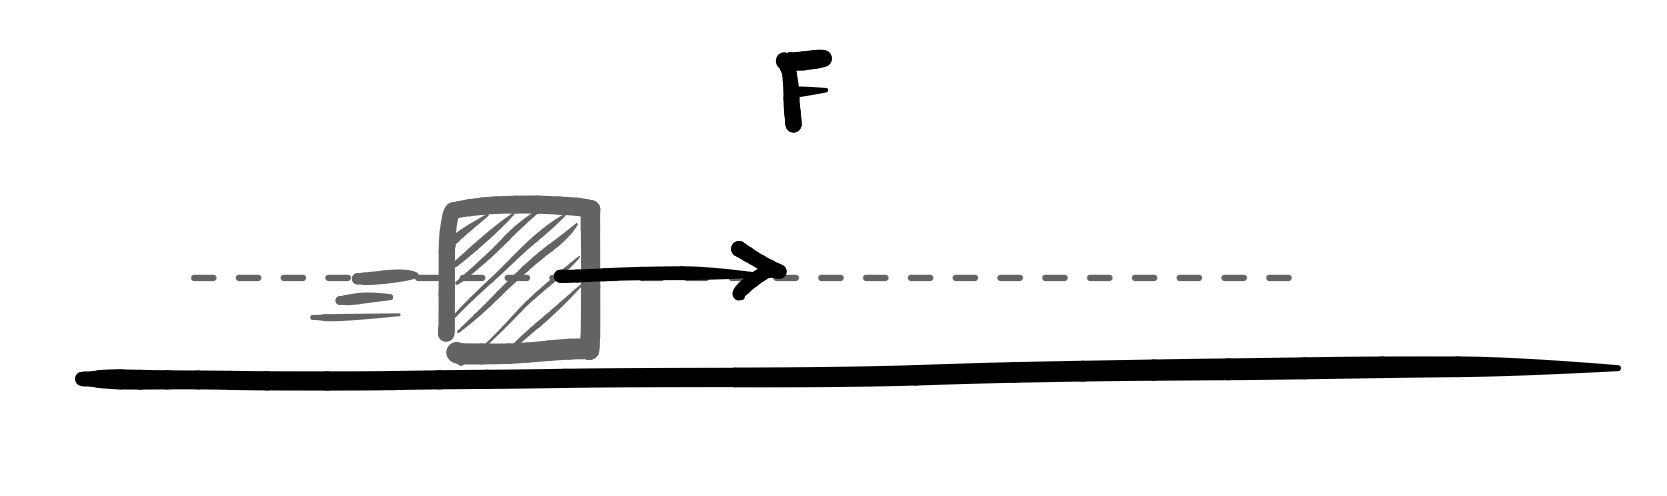
\includegraphics[width=0.5\linewidth]{imagensdinamicanewton/impulsoqdm01.png}};
  \end{scope}
\end{tikzpicture}
\captionof{figure}{O impulso de uma força $\vec F.$}
\label{fig_newton_impulsoqdm01}
} 
\vspace{0.3cm}




Ao mesmo tempo, quanto maior for o valor da força $\vec F$ em si, maior será a mudança de movimento gerada na caixa. Sendo assim, o impulso consegue armazenar as duas grandezas que influenciam na mudança de movimento da caixa: a força que a empurra e o intervalo de tempo ao longo do qual tal força atua.


\secgfe{Onde é usada}

O conceito de impulso pode ser usado em quaisquer problemas de dinâmica. Na verdade, é possível resolver qualquer problema de dinâmica usando apenas os conceitos de força e aceleração, como já fizemos. Contudo, é possível também resolvê-los usando a linguagem de impulso e momento linear, como veremos. Essa última linguagem será mais útil e interessante de se usar em problemas que envolvam colisões de corpos, como ficará claro em breve.

Considere, por exemplo, a situação em que se tem uma caixa de massa $m=5$ kg, em repouso sobre um solo horizontal sem atrito, como na situação da Figura \ref{fig_newton_impulsoqdm01}. Se uma força horizontal $F=20$N começa a acelerá-la, qual é a velocidade final da caixa após $3$ segundos?

Perceba que temos dois caminhos para resolver este problema. 


\begin{enumerate}
    \item Leis de Newton e Cinemática.

    Aqui, usamos a Segunda Lei de Newton para encontrar a aceleração da caixa:

    $$ F_{\text{R}} = ma \implies 20 = 5a \implies a = 4 \text{m/s}^2. $$

    Agora, munidos da aceleração, e em se tratar de um MUV, podemos usar a Equação \eqref{mecanica_eq_muvfuncaovelocidade} para computar sua velocidade:

    $$ v= \cancelto{0}{v_0} + at \implies v(t) = 4t \implies v(3) = 12 \text{ m/s.} $$

     \item O conceito de impulso.

     Podemos computar inicialmente o impulso gerado pela força $\vec F:$

     $$I = F \cdot \Delta t \implies I = 20 \text{N} \cdot 3 \text{s} = 60 \text{N}\cdot \text{s}.$$

     Da última relação da Equação \eqref{eq_newton_impulsointermediario}, temos:


     $$ I = m \Delta v \implies 60 \text{N}\cdot \text{s} = 5 \text{kg} \cdot \Delta v \implies \Delta v = 12 \text{m/s}, $$
     
    \noindent ou seja, por meio do impulso foi possível computar a variação total de movimento gerado na caixa: ela foi de 12 m/s. Como a caixa começou do repouso, isso implica que sua velocidade final será exatamente de 12 m/s, concordando com o cálculo anteriormente feito.
     
\end{enumerate}

Por ora, parece que estamos criando algo um tanto quanto desnecessário: apenas uma forma de complicar as coisas que já sabíamos. Contudo, no desenvolvimento da Equação \eqref{eq_newton_convervacaomomentolinear}, veremos algumas vantagens em trabalhar com a linguagem do impulso e momento linear.

\secgfe{Erros comuns}

O erro mais comum aqui é ignorar o caráter vetorial do impulso. A própria Equação \eqref{eq_newton_impulso} deixa evidente que o impulso é uma grandeza vetorial, que aponta na mesma direção e sentido que a força $\vec F.$

Assim, da mesma forma que forças em sentidos opostas geram acelerações em sentidos opostos -- que possuirão sinais diferentes --, essas mesmas forças em direções opostas gerarão impulsos em direções opostas, que levarão, portanto, sinais distintos: um será positivo e o outro negativo.


\secgfe{Observações}

Cabem duas observações importantes aqui sobre a Equação \eqref{eq_newton_impulso}. A primeira, mais simples, é sobre sua unidade de medida que, no S.I, será

$$ [I] = [F][\Delta t] = \text{N}\cdot \text{s},$$

\noindent que não recebe um nome especial e é lido dessa forma mesmo: newton vezes segundo.

A segunda observação é que a Equação \eqref{eq_newton_impulso} só se propõe a calcular o impulso de uma força constante. Afinal de contas, caso a força varie o tempo inteiro, qual valor de $F$ colocaríamos em tal equação?

Pois bem. No caso de uma força variável, o impulso é computado pela área abaixo do gráfico de \textbf{Força vs Tempo}, como ilustra a Figura \ref{fig_newton_impulsoqdmgraficofvst1} e como pode ser entendido em mais detalhes no Apêndice \ref{apendice_areagraficovxt}.


\vspace{0.3cm}
{
\centering
\begin{tikzpicture}
  \begin{scope}[blend mode=multiply]
    \node {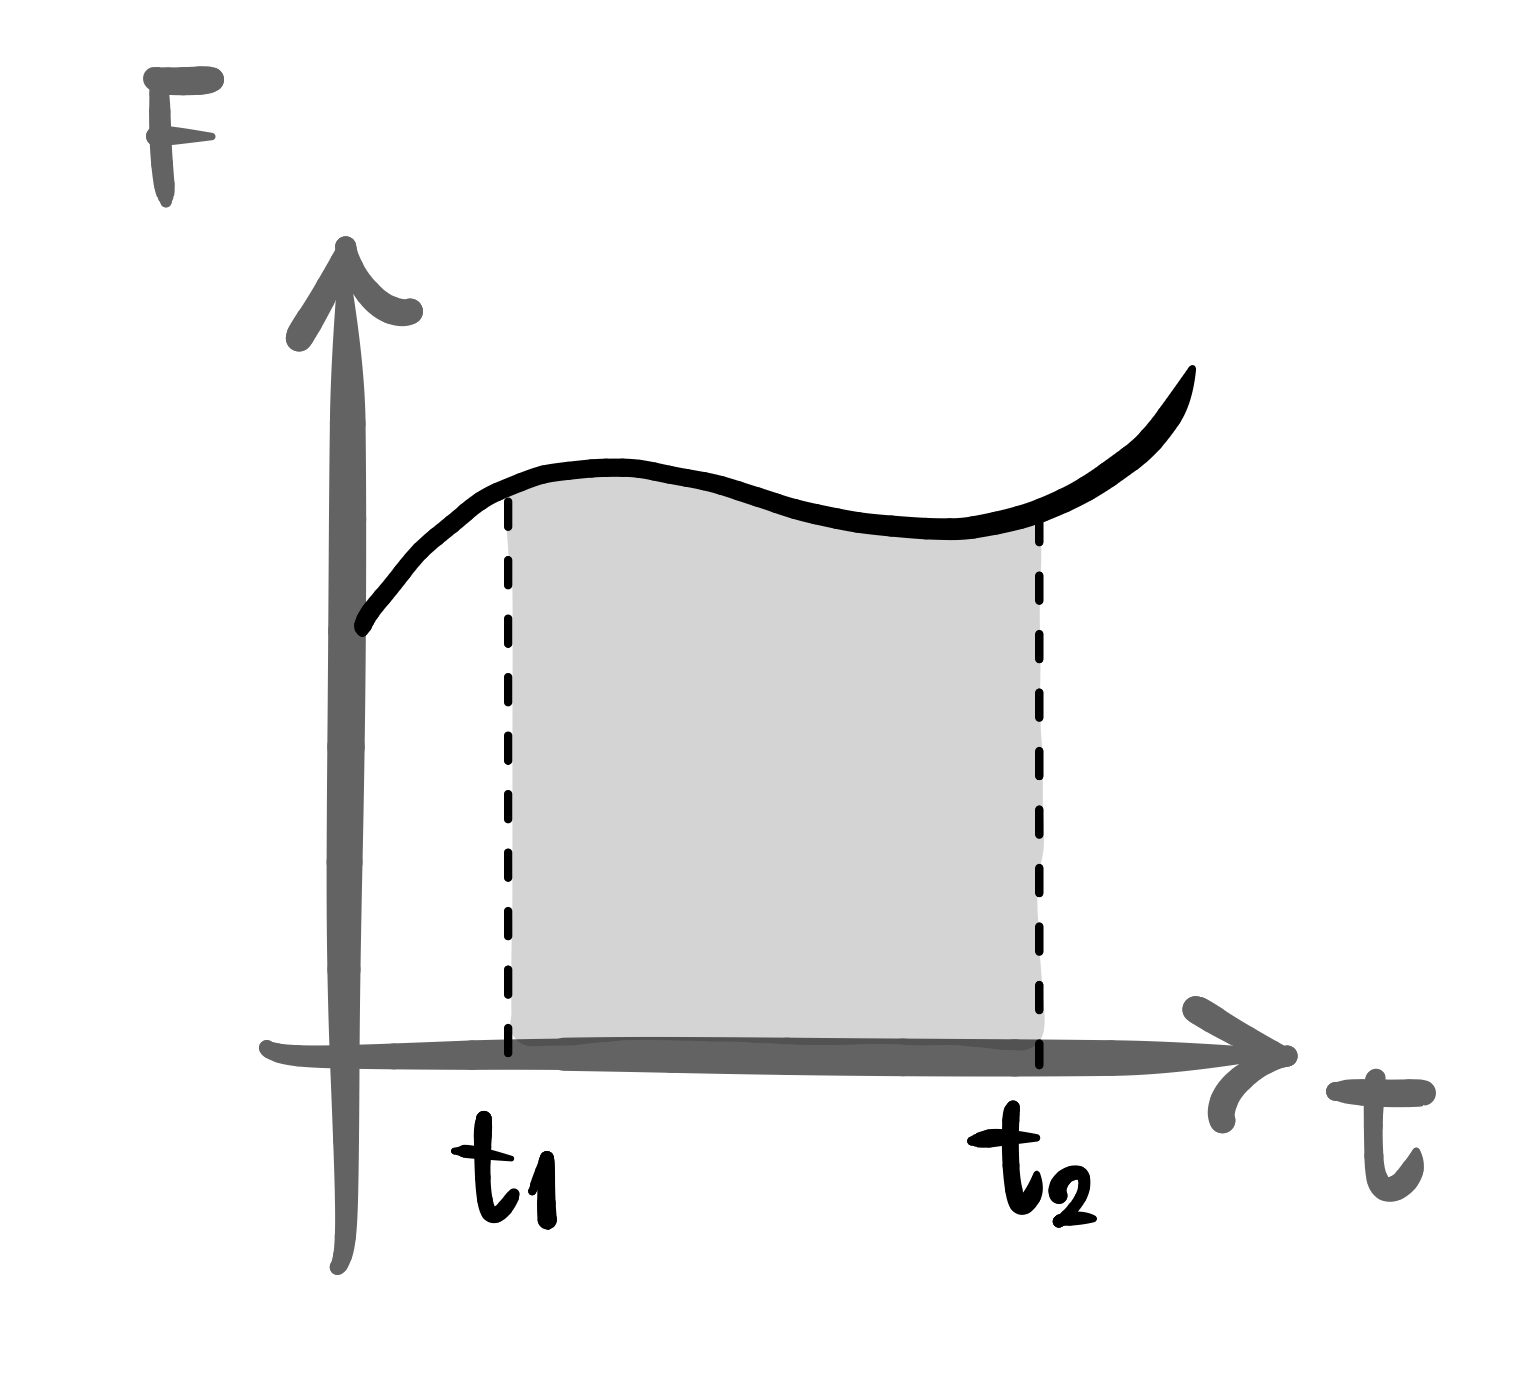
\includegraphics[width=0.3\linewidth]{imagensdinamicanewton/impulsograficofvst2.png}};
  \end{scope}
\end{tikzpicture}
\captionof{figure}{O impulso que a força $F$ gera na partícula que sofre a atuação de tal força é, entre os instantes $t_1$ e $t_2,$ dado pela área abaixo da curva $F(t)$ entre tais instantes.}
\label{fig_newton_impulsoqdmgraficofvst1}
} 
\vspace{0.3cm}



\vspace{0.3cm}


\begin{exemplo}[Nível I]\label{exemplo_newton_impulso}

Considere um tenista que bate com sua raquete em uma bola de tênis. Se a força exercida pelo tenista é de $F=200$N e o tempo de contato da bola com a raquete é de $0.02$ segundos, calcule o impulso que tal força gera na bolinha.

\resolucao

O impulso pode ser calculado de forma imediata pela aplicação da Equação \eqref{eq_newton_impulso}:

$$ I = F \Delta t = 200\text{N} \cdot 0.02s = 4 \text{N}\cdot \text{s}. $$

\end{exemplo}


\vspace{0.3cm}




\begin{exemplo}[Nível II]\label{exemplo_newton_impulso}

Uma força $F$ atua em uma partícula de massa $m=2$ kg. A força $F$ varia no tempo, sendo tal variação representada pelo gráfico da Figura \ref{fig_newton_impulsoqdmgraficofvst2}, em que a curva da força ao longo do tempo é uma semi-circunferência.

\vspace{0.3cm}
{
\centering
\begin{tikzpicture}
  \begin{scope}[blend mode=multiply]
    \node {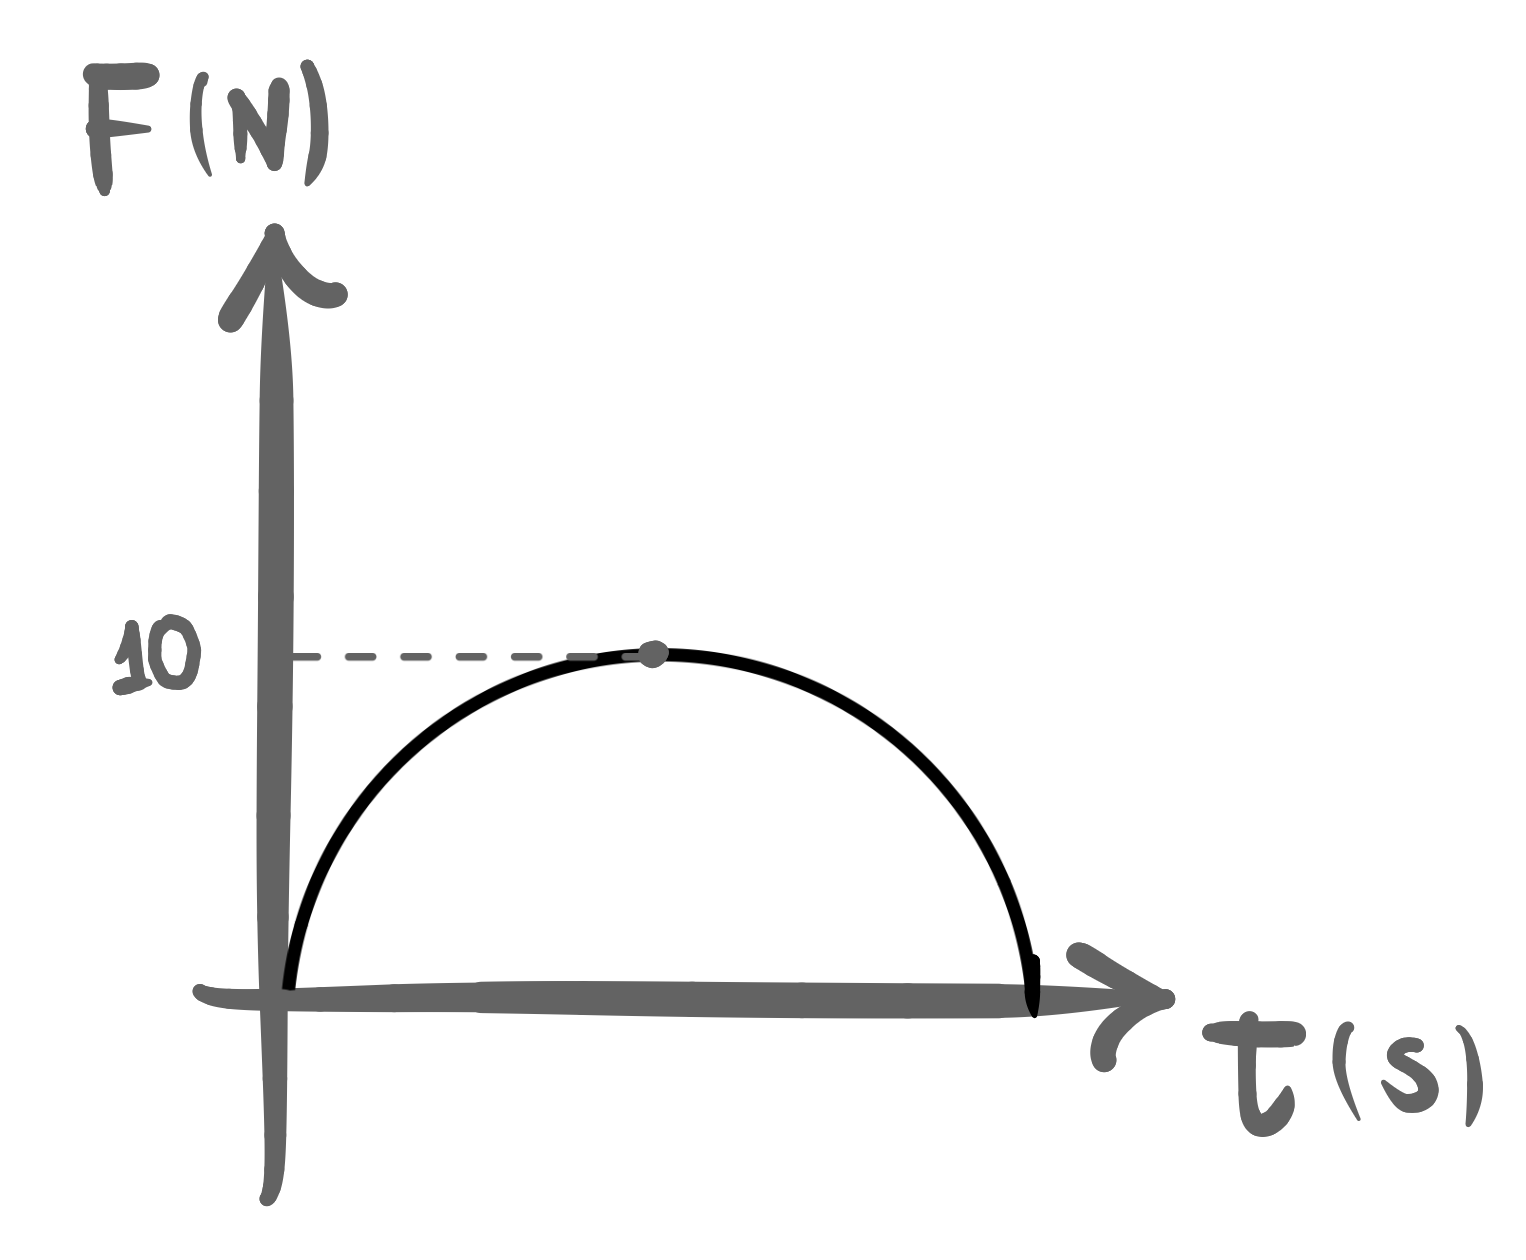
\includegraphics[width=0.3\linewidth]{imagensdinamicanewton/impulsograficofvst1.png}};
  \end{scope}
\end{tikzpicture}
\captionof{figure}{}
\label{fig_newton_impulsoqdmgraficofvst2}
} 
\vspace{0.3cm}

Calcule a variação de velocidade gerada na partícula ao longo trecho inteiro de movimento devido à ação de tal força.

\resolucao

Podemos calcular o impulso pela área abaixo do gráfico da Figura \ref{fig_newton_impulsoqdmgraficofvst2}. Sendo o raio da semicircunferência igual a 10, temos

$$ I = \dfrac{1}{2} \pi R^2 = 50 \pi \text{ N}\cdot \text{s}. $$

Ao mesmo tempo, pela última relação da Equação \eqref{eq_newton_impulsointermediario}, temos que

$$ I = m \Delta v \implies 50 \pi \text{ N}\cdot \text{s} = 2 \text{kg} \cdot \Delta v \implies \boxed{\Delta v =25 \pi \text{ m/s} \approx 78 \text{ m/s}.} $$

\end{exemplo}

\vspace{0.3cm}











\begin{secnivel}[Teorema do Impulso]{I}{Teorema do Impulso}
  
  \eqLdois{dem}{eq_newton_teoremaimpulso}{\vec I = \Delta \vec p.}

\end{secnivel}







\secgfe{De onde vem}

A Equação \eqref{eq_newton_teoremaimpulso} é pura e simplesmente a Segunda Lei de Newton, porém escrita em termos das novas grandezas que definimos: impulso e momento linear. É fácil mostrar isso, como segue:

$$\vec F = m \vec a \implies \vec F = m \dfrac{\Delta \vec v}{\Delta t} \implies  \vec F \cdot \Delta t = m \Delta \vec v.$$



Note, na última relação acima, que o lado esquerdo é justamente o impulso $\vec I$ da força $\vec F,$ dado pela Equação \eqref{eq_newton_impulso}. Já o lado direito representa a variação do momento linear da partícula:

\begin{align}
    \Delta \vec p &=\vec p_f - \vec p_0 \nonumber \\
    &= m \vec v_f - m \vec v_0  \nonumber \\
     &= m(\vec v_f - \vec v_0)  \nonumber \\
      &= m \Delta \vec v.  \nonumber
\end{align}



% $$ \Delta \vec p = \vec p_f - \vec p_0 = m \vec v_f - m \vec v_0 = m(\vec v_f - \vec v_0) = m \Delta \vec v.$$

Assim, temos

\begin{align}
    \vec F \cdot \Delta t &= m \Delta \vec v \nonumber \\
    \vec I &= \Delta \vec p, \nonumber
\end{align}

\noindent como queríamos demonstrar.


\secgfe{Onde é usada}

Como a Equação \eqref{eq_newton_teoremaimpulso} é exatamente a Segunda Lei de Newton, ela pode ser usada para resolver quaisquer problemas que antes resolvíamos usando a Equação \eqref{eq_dinamica1_segundaleinewton}.  É importante destacar que a Equação \eqref{eq_newton_teoremaimpulso} não possui absolutamente nenhum conteúdo ou informação a mais que a Segunda Lei de Newton: trata-se exatamente do mesmo conteúdo físico, porém reescrito em termos das novas grandezas.

Assim, qualquer problema de dinâmica que pode ser resolvido por meio da Segunda Lei de Newton pode, também, ser resolvido por meio do Teorema do Impulso. Contudo, será mais comum usarmos a última opção em problemas sobre colisões, e o principal motivo para tal ficará evidente no desenvolvimento da Equação \eqref{eq_newton_convervacaomomentolinear}.


\secgfe{Erros comuns}

Um erro comum é o estudante acabar confundindo impulso com força. Lembre-se de que a força é algo local, que atua na partícula em cada instante de tempo. Já o impulso mede o efeito da força acumulado ao longo do tempo: tal efeito é causar a variação do momento da partícula -- é exatamente isso que diz a Equação \eqref{eq_newton_teoremaimpulso}.


Para além disso, os erros mais comuns aqui são os mesmos cometidos nas Equações \eqref{eq_newton_momentolinear} e \eqref{eq_newton_impulso}: ignorar o caráter vetorial das grandezas impulso e momento linear.


\secgfe{Observações}

A Equação \eqref{eq_newton_teoremaimpulso} nos diz que, para gerar uma mesma variação de movimento (momento linear) em um corpo, isto, é, para produzir um mesmo $\Delta \vec p,$ podemos fazê-lo de duas formas diferentes:

\begin{enumerate}
    \item [(i)] usando uma força $F$ intensa em um curto intervalo de tempo $\Delta t,$ que geraria um impulso

     $$ I = F \cdot \Delta t;$$

     \item [(ii)] ou usando uma força, digamos, 10 vezes menor, $\sfrac{F}{10}$, durante um intervalo de tempo 10 vezes maior, isto é, $10 \Delta t:$

     $$ I' = F'\Delta t'=  \dfrac{F}{\cancel {10}} \cdot \cancel {10} \Delta t = F \Delta t = I.$$

     Ou seja, nos dois casos, gera-se o mesmo impulso e, como diz a Equação \eqref{eq_newton_teoremaimpulso}, sendo o impulso o agente responsável pela variação do momento linear, nos dois casos produz-se a mesma variação de momento.
\end{enumerate}

Em outras palavras, uma força muito intensa aplicada durante um intervalo extremamente curto pode produzir exatamente o mesmo efeito que uma força bem menor aplicada por um tempo maior. O que realmente importa é o produto entre força e tempo -- o impulso.

Isso aparece de forma clara em diversas situações do cotidiano. Em um acidente de carro, por exemplo, o airbag não “reduz” necessariamente o impulso total envolvido na colisão, mas o distribui ao longo de um intervalo de tempo maior. Ao inflar, ele faz com que o corpo do passageiro demore mais para parar, diminuindo a intensidade da força média sofrida pelo fato de fazê-la atuar em um maior intervalo de tempo. Assim, com o airbag, apesar de você sofrer a mesma variação de movimento total (você terminará em repouso após a colisão com ou sem airbags), você sente uma força menor desacelerando-o, o que torna mais suave o impacto, que ficou diluído no tempo.

O mesmo princípio está presente em amortecedores de veículos, que evitam impactos bruscos ao prolongar o tempo de interação com o solo, e também nos esportes: ao receber uma bola de basquete, um jogador experiente recua as mãos, “acompanhando” o movimento. Com isso, ele aumenta o tempo de contato e reduz a força sentida, mesmo realizando a mesma variação de movimento da bola.


\vspace{0.3cm}


\begin{exemplo}[Nível I]\label{exemplo_newton_teoremaimpulsoex01}

Considere a situação da Figura \ref{fig_newton_momentolinear02}, em que temos a bola de massa $3$kg colidindo contra a parede. Mediu-se o tempo de colisão da bola com a parede, que foi de $200$ms. Qual foi a força média exercida pela parede sob a bola?

\resolucao

Podemos resolver esse problema de duas formas, as quais detalharemos aqui, a fim de tornar claro para o leitor as suas diferenças.

\begin{enumerate}
    \item [(i)] Solução pelo Teorema do Impulso

    Vamos adotar agora um sistema de referência orientado para a esquerda, isto é, velocidades, acelerações, forças e quaisquer outras grandezas vetoriais serão positivas quando orientadas para a esquerda.

    O momento linear inicial da partícula é $p_0=mv_0= 3 \cdot 5=  15 \text{kg} \cdot \text{m/s}.$ O seu momento linear após a colisão é $p_f=mv_f= 3 \cdot (-5)=  -15 \text{kg} \cdot \text{m/s},$ de modo que a variação do momento é

    $$ \Delta p = p_f - p_0 = -15 - 15 = -30 \text{kg} \cdot \text{m/s}.$$

    Assim, por meio do Teorema do Impulso, temos

$$  I = F \Delta t = \Delta p \implies F \cdot 0.2 = -30 \text{kg} \cdot \text{m/s} \implies \boxed{F = -150 \text{N}}. $$

Note que usamos o tempo de colisão $\Delta t = 200$ ms = $200 \cdot 10^{-3}$ s = $ 0.2$s. Segundo nossa convenção, uma força negativa é uma força orientada para a direita, o que está condizente com o esperado: no colisão a parede ``empurra'' a bolinha para a direita. Assim, a força média\footnote{Dizemos força média porque nada nos garante que, ao longo dos dois décimos de segundo durante a colisão, a força não varie. Ela pode, mesmo em um intervalo de tempo muito curto, ser variável. O cálculo que fizemos calcula o valor da força média neste intervalo: uma força que, caso se mantivesse constante durante os mesmos dois décimos de segundo, geraria o mesmo efeito.} feita pela parede na bolinha é de 150N, orientada para a direita.
    


    \item [(ii)] Solução pela Segunda Lei de Newton

    Para resolver o problema usando a Segunda Lei de Newton começamos computando a aceleração média que a bolinha sofre durante a colisão, mantendo o mesmo referencial em que o sentido positivo é para a esquerda:

    $$ a = \dfrac{\Delta v}{\Delta t} = \dfrac{v_f-v_0}{200 \text{ms}} = \dfrac{-5-5}{0.2 \text{s}} =-50 \text{m/s}^2,$$

    \noindent em que o sinal negativo indica sua orientação: para a direita, como esperado.

    Agora, munidos da aceleração, é fácil computar a força necessária para gerá-la: é o que faz a Segunda Lei de Newton, que nos fornece

    $$ F = ma = 3 \text{kg} \cdot (-50\text{m/s}^2) = -150 \text{N},$$

    \noindent em que o sinal, novamente, indica apenas o sentido da força de acordo com a nossa orientação adotada. Como era esperado, chegamos exatamente no mesmo resultado.
    
\end{enumerate}


\end{exemplo}


\vspace{0.3cm}


\begin{exemplo}[Nível II]\label{exemplo_newton_teoremaimpulsoex02}

Em um jogo de sinuca, após uma tacada, uma das bolas, que se move inicialmente com velocidade de $30$ m/s, colide com uma das paredes da mesa, como ilustrado na Figura \ref{fig_newton_impulsoteoremacolisao2d01}.

\vspace{0.3cm}
{
\centering
\begin{tikzpicture}
  \begin{scope}[blend mode=multiply]
    \node {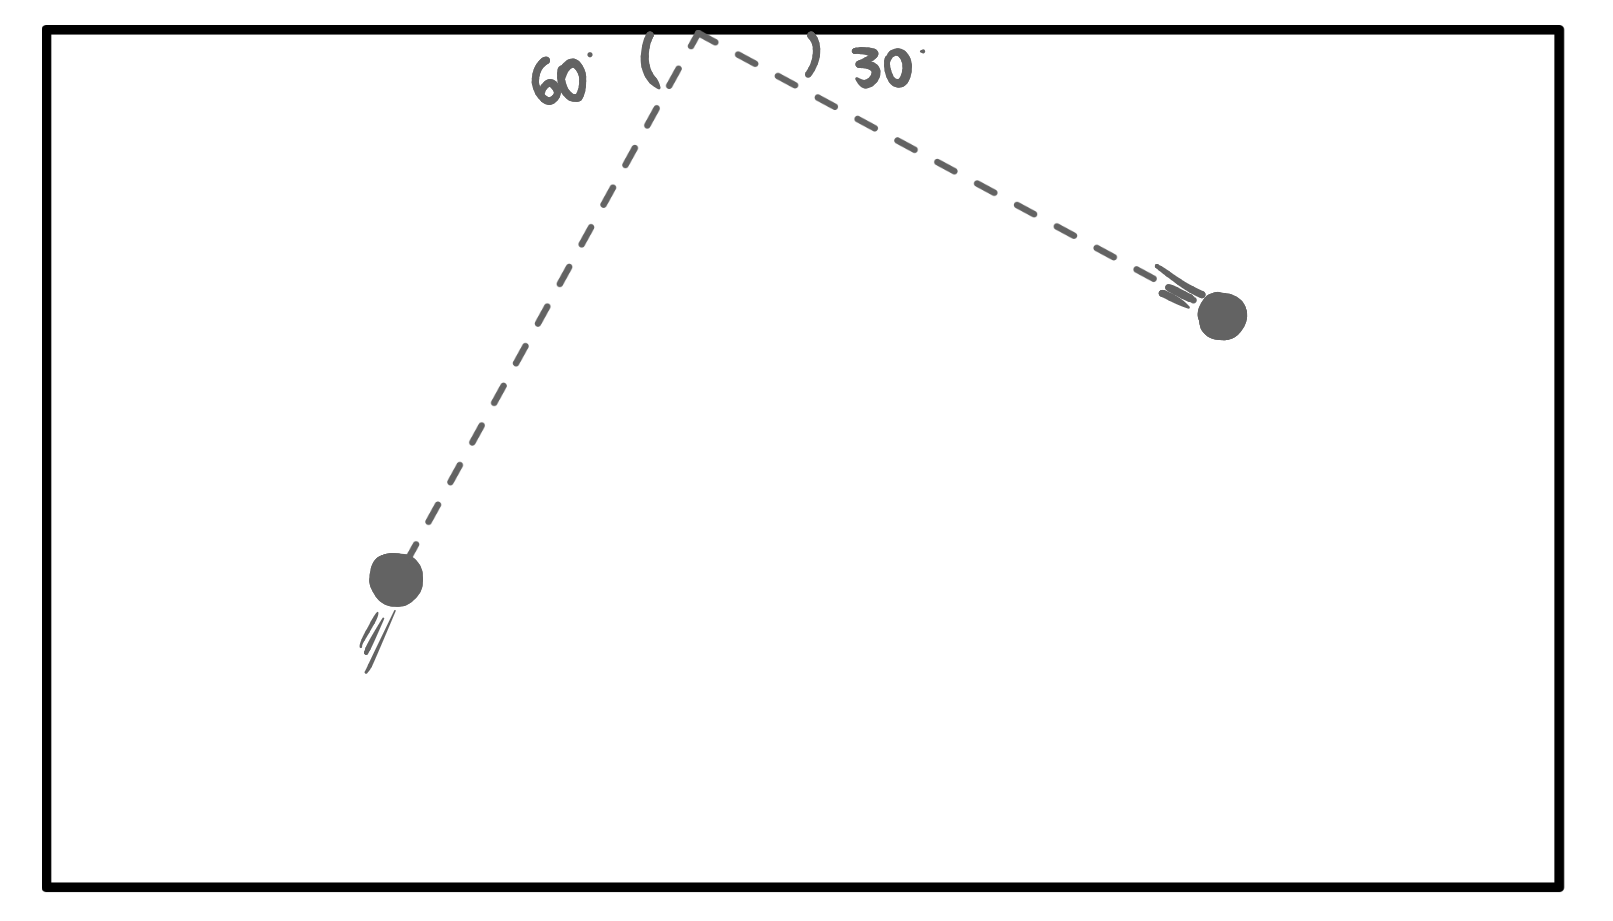
\includegraphics[width=0.5\linewidth]{imagensdinamicanewton/teoremaimpulsocolisao2d1.png}};
  \end{scope}
\end{tikzpicture}
\captionof{figure}{}
\label{fig_newton_impulsoteoremacolisao2d01}
} 
\vspace{0.3cm}

Após a colisão, a bola sai com uma velocidade de módulo igual a $10\sqrt 3$ m/s, porém em uma direção distinta, como mostra a figura. Se o tempo de colisão foi de 100ms e a massa da bola em questão é de 100g, pede-se responder:


\begin{enumerate}
    \item [a)] o módulo da força média feita pela parede na bola durante a colisão.

    \item [b)] houve atrito durante o choque?
\end{enumerate}


\resolucao

\begin{enumerate}
    \item [a)] O módulo do momento linear da bolinha é, antes e depois da colisão, dado por:

\begin{align}
    p_0 & = mv_0 = 0.1 \text{kg} \cdot 30 \text{m/s} = 3 \text{kg} \cdot \text{m/s} \nonumber \\
    p_f & = mv_f =  0.1 \text{kg} \cdot 10\sqrt 3 \text{m/s} = \sqrt 3 \text{kg} \cdot \text{m/s}. \nonumber
\end{align}

A Figura \ref{fig_newton_impulsoteoremacolisao2d02} mostra a disposição geométrica dos vetores $\vec p_f$ e $-\vec p_0$ para o cálculo do módulo do impulso $\vec{I}$, que é dado, pela Equação \eqref{eq_newton_teoremaimpulso}, pela variação do momento linear:

$$ \vec I = \Delta \vec p = \vec p_f - \vec p_0.$$


{
\centering
\begin{tikzpicture}
  \begin{scope}[blend mode=multiply]
    \node {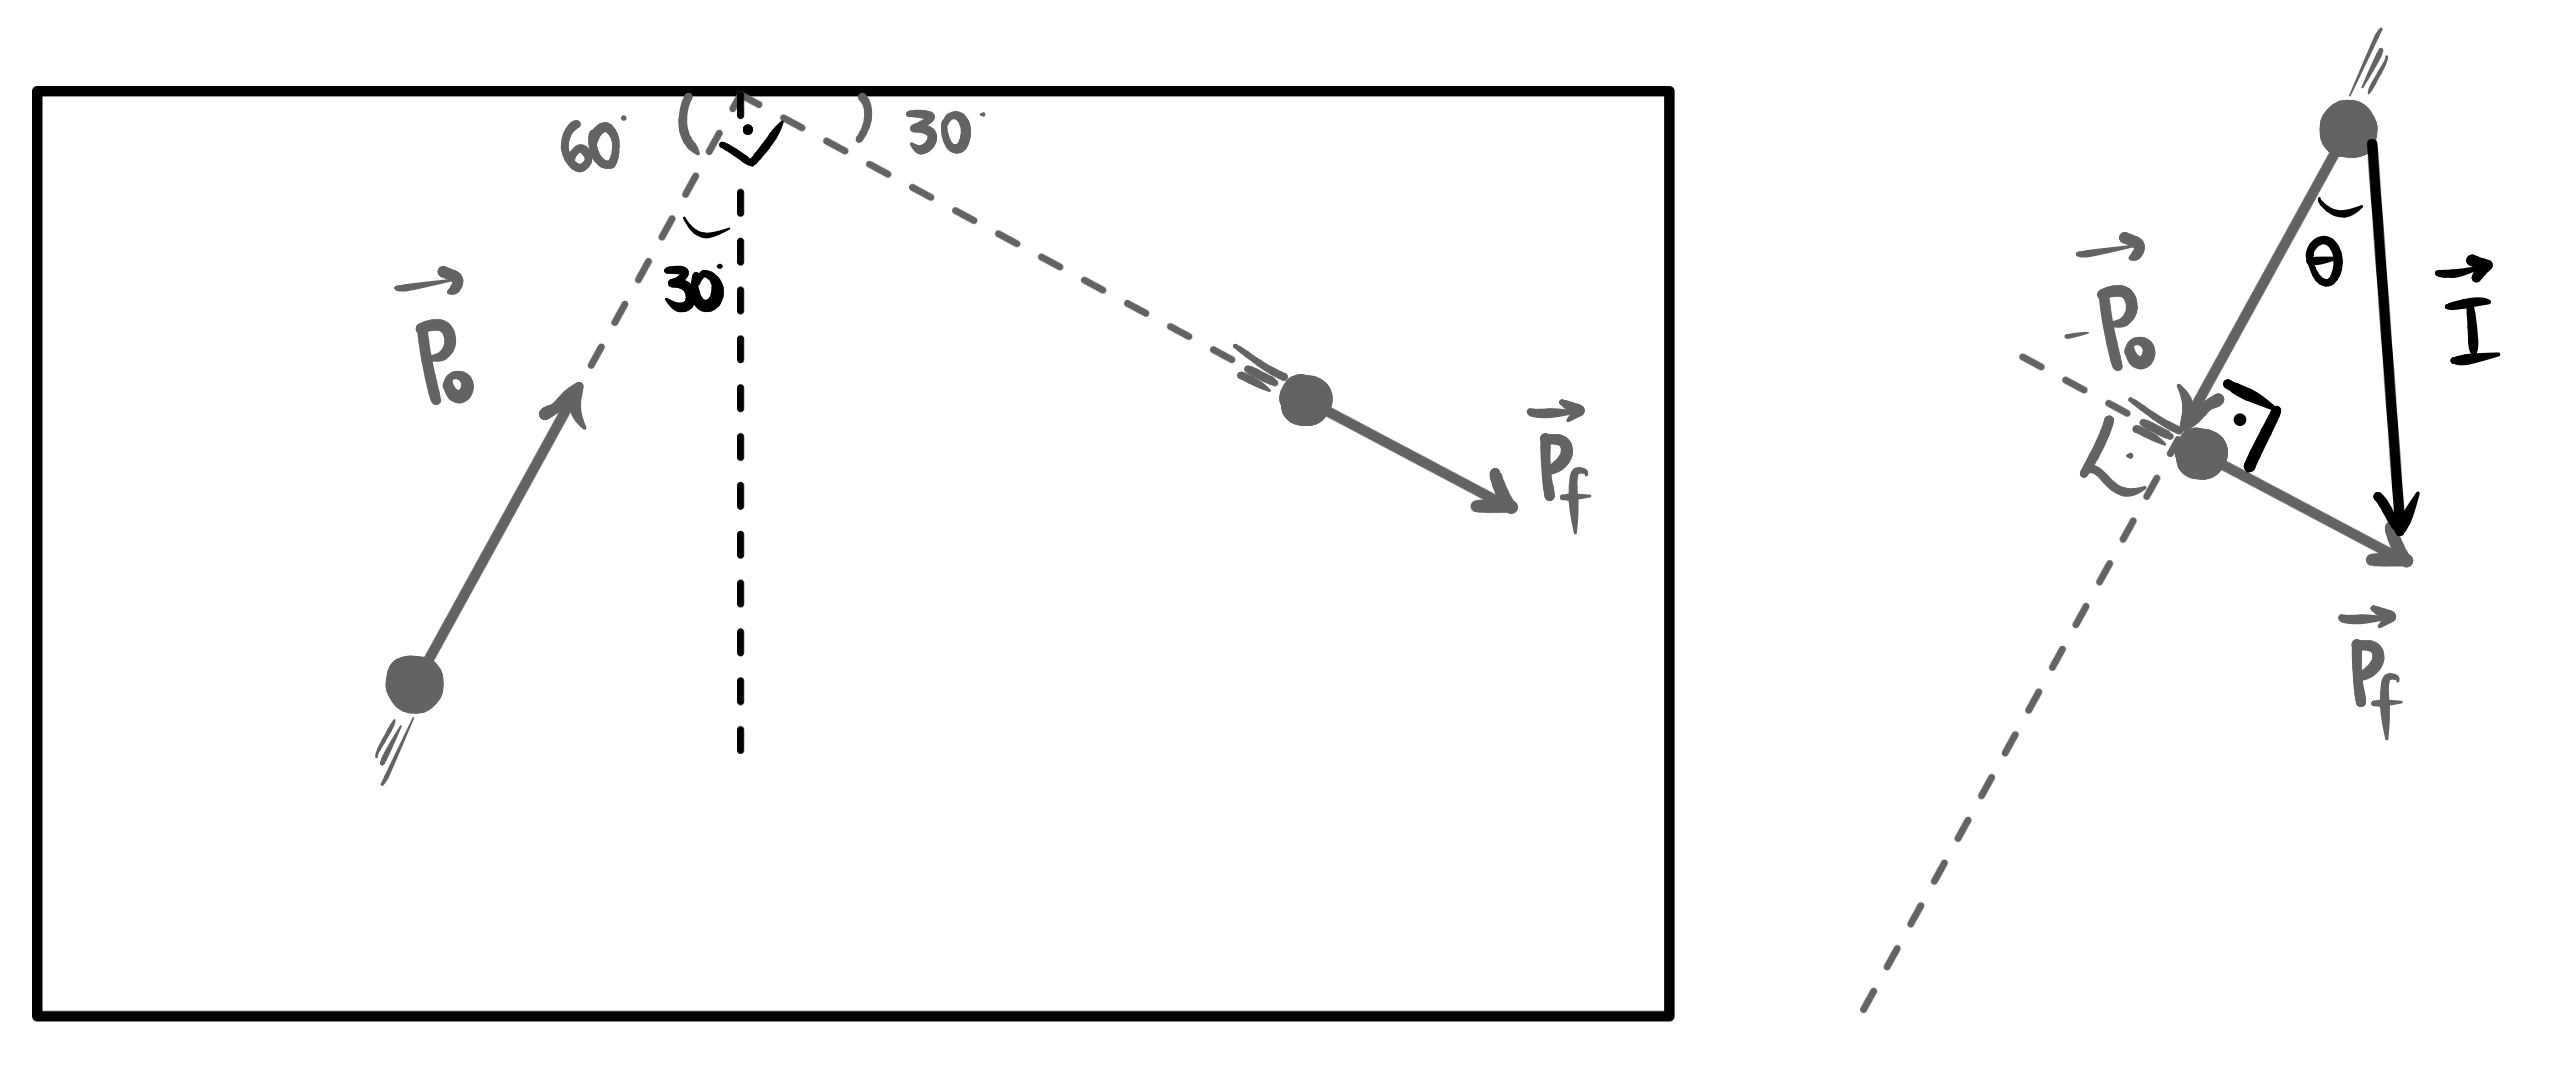
\includegraphics[width=0.75\linewidth]{imagensdinamicanewton/teoremaimpulsocolisao2d2.png}};
  \end{scope}
\end{tikzpicture}
\captionof{figure}{}
\label{fig_newton_impulsoteoremacolisao2d02}
} 
\vspace{0.3cm}

Como os vetores $\vec p_0$ e $\vec p_f$ são perpendiculares, o triângulo no lado direito da Figura \ref{fig_newton_impulsoteoremacolisao2d02} é retângulo, de modo que vale o Teorema de Pitágoras:

$$ I^2 = p_0^2 + p_f^2 = 3^2+ \sqrt 3^2 = 12 \implies I = 2 \sqrt 3 \text{N} \cdot \text{s}.$$

Assim, pela definição de impulso feita na Equação \eqref{eq_newton_impulso}, tem-se

$$ I = F \Delta t \implies 2 \sqrt 3 \text{N} \cdot \text{s} = F \cdot 0.1 \text{s} \implies \boxed{F = 20 \sqrt 3  \text{N} \approx 35 \text{N,} }  $$

\noindent de modo que a força média feita pela mesa sob a bolinha, durante o curto intervalo do choque, é de aproximadamente 35N.



    \item [b)] Sabemos que as forças trocadas entre duas superfícies podem ser de dois tipos: forças de compressão (força normal), que são perpendiculares à superfície de contato; ou forças tangenciais (força de atrito), que são paralelas à superfície de contato. Sendo assim, para avaliar o tipo de força que atuou durante o contato, basta avaliar suas componentes: haverá atrito caso a força computada no item anterior tenha alguma componente tangencial, isto é, paralela à superfície de contato.

    Note, no desenho da esquerda Figura \ref{fig_newton_impulsoteoremacolisao2d02}, que o ângulo entre o vetor $\vec p_0$ e a direção perpendicular à parede da mesa (linha pontilhada vertical) é de $30^\circ$. Avaliando agora o triângulo no lado direto da figura, vemos que o ângulo entre o vetor $\vec p _0$ e a direção do impulso (e, consequentemente, a direção da força $\vec F$ feita pela mesa na bolinha) é o ângulo $\theta$ tal que
    $$ \tan \theta = \dfrac{p_f}{p_0} = \dfrac{\sqrt 3}{3} \implies \theta = 30^\circ.$$

    Ou seja, o ângulo entre o vetor $\vec p _0$ e a força $\vec F$ é o mesmo ângulo entre o vetor $\vec p _0$ e a direção normal; logo, conclui-se que a força $\vec F$ é paralela à direção normal. Não havendo componentes da força de contato paralelas à superfície, não houve atrito. O impulso aponta na direção normal à parede (perpendicular à superfície de contato), confirmando que a força exercida pela mesa foi 100\% normal.
    
\end{enumerate}


\end{exemplo}


\vspace{0.3cm}









\begin{secnivel}[Conservação do Momento Linear]{I}{Lei da Conservação do Momento Linear}
  
Em um sistema isolado de forças externas, vale que


\eqLdois{dem}{eq_newton_convervacaomomentolinear}{\Delta \vec p_{\text{sistema}} = \vec 0.}

\end{secnivel}







\secgfe{De onde vem}

Tal equação, na verdade, é a principal razão de termos definido as grandezas impulso e momento linear. Ela diz que o momento linear de um sistema isolado de forças externas se conserva, ou seja, ele não varia: é uma grandeza que se preserva.

É importante entender, primeiro, o que são forças internas e externas a um certo sistema. Tal tarefa exige que determinemos, primeiro, quais são as partículas do nosso sistema.

Considere, por exemplo, a situação da Figura \ref{fig_newton_conservacaoqdm01}, que mostra dois carros que irão colidir. Neste caso, nosso sistema é composto pelos carros $A$ e $B$: desejamos estudar como a interação (colisão) irá afetar o movimento de cada um deles, e como eles se moverão logo em seguida.


\vspace{0.3cm}
{
\centering
\begin{tikzpicture}
  \begin{scope}[blend mode=multiply]
    \node {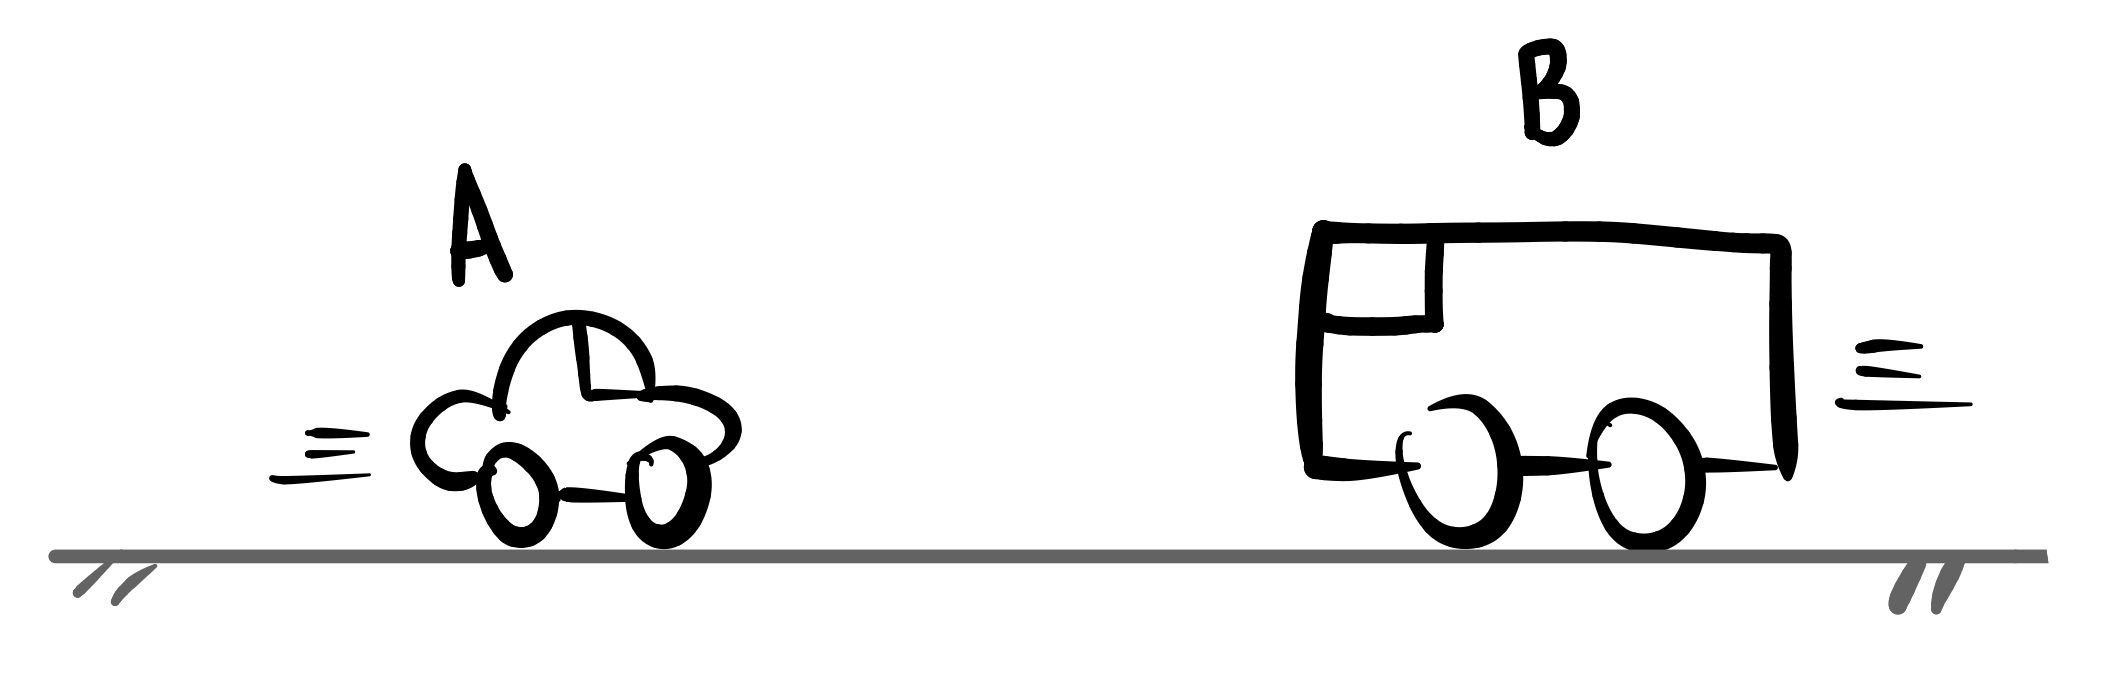
\includegraphics[width=0.5\linewidth]{imagensdinamicanewton/conservacaoqdm01.png}};
  \end{scope}
\end{tikzpicture}
\captionof{figure}{Ao estudar o movimento das partículas $A$ e $B$ o sistema em questão é aquele composto por tais partículas.}
\label{fig_newton_conservacaoqdm01}
} 
\vspace{0.3cm}



Munidos da informação do item acima, dizemos que uma força é interna a um sistema quando ela é feita por um elemento de tal sistema. Ou seja, ainda na situação da Figura \ref{fig_newton_conservacaoqdm01}, note que teremos diversas forças. Classifiquemo-las:

\begin{enumerate}
    \item [(i)] Forças Externas

São aquelas realizadas por agentes externos ao sistema, ou seja, por qualquer agente que não seja o carro $A$ ou $B$. Entre elas estão:
          \begin{enumerate}
          
              \item Atrito: serão forças realizadas pelo solo (agente externo) nos carros (elementos internos do nosso sistema).
              \item Força normal: são forças também realizadas pelo solo (agente externo) nos carros (elementos internos do nosso sistema).
              \item Forças peso: são forças realizadas pela Terra (agente externo) nos carros (elementos internos do nosso sistema).
              \item Força de resistência do ar: são forças realizadas pelas partículas de ar (agente externo) nos carros (elementos internos do nosso sistema).
          \end{enumerate}

        \item [(ii)] Forças Internas

         Serão aquelas forças feitas por elementos do sistema em elementos do sistema. Ou seja, no caso de uma colisão, o carro $A$ baterá no $B$ e, pela Terceira Lei de Newton, o carro $B$ baterá com a mesma força em $A$. Esse par de forças é interno ao sistema dos corpos $A$ e $B$. A Figura \ref{fig_newton_conservacaoqdm02} ilustra tal situação.

\vspace{0.3cm}
{
\centering
\begin{tikzpicture}
  \begin{scope}[blend mode=multiply]
    \node {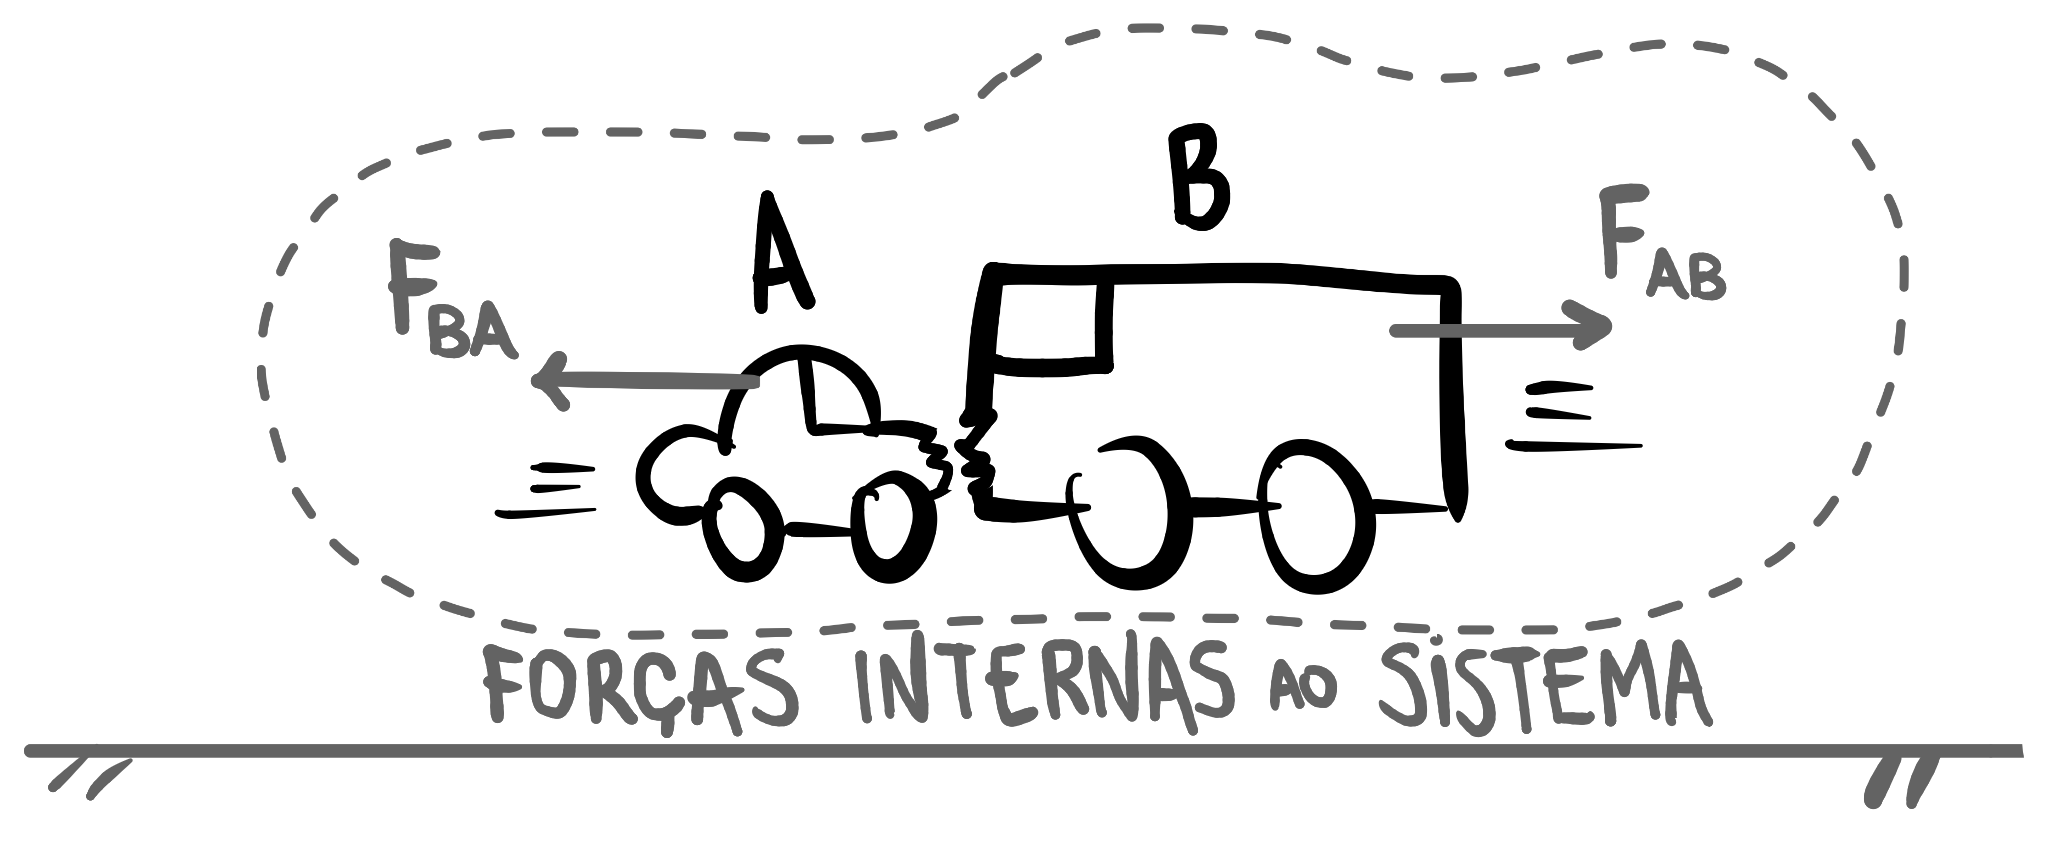
\includegraphics[width=0.5\linewidth]{imagensdinamicanewton/conservacaoqdm02.png}};
  \end{scope}
\end{tikzpicture}
\captionof{figure}{As forças internas ao sistema composto pelas partículas $A$ e $B$ são aquelas feitas por partículas internas ao sistema em partículas do próprio sistema. }
\label{fig_newton_conservacaoqdm02}
} 
\vspace{0.3cm}


         Considere, por exemplo, um sistema de três partículas $A$, $B$ e $C.$ As forças internas a tal sistema seriam, por exemplo, as forças trocadas entre $A$ e $B;$ entre $A$ e $C$ e entre $B$ e $C$. Cada uma dessas virá aos pares, pela Terceira lei de Newton: das forças trocadas entre $A$ e $B$ teremos $F_{\text{AB}}$, a força de $A$ em $B,$ e $F_{\text{BA}},$ a reação, que é a força de $B$ em $A.$
 
        
\end{enumerate}

Sendo assim, a Equação \eqref{eq_newton_convervacaomomentolinear} diz que, na ausência de forças externas, o momento linear total de um sistema é conservado. O momento linear total de um sistema é, naturalmente, a soma dos momentos lineares de todas as partículas do sistema, como mostra a Figura \ref{fig_newton_conservacaoqdm03}. Matematicamente, se um certo sistema é composto pela partículas $1,2,3, \dots,n$, então o momento linear total do sistema é 

$$ \vec p_{\text{sistema}} = \vec p_1 + \vec p_2 + \vec p_3 + \dots + \vec p_n,$$

\noindent em que $\vec p_i$ representa o momento linear da i-ésima partícula do sistema.

\vspace{0.3cm}
{
\centering
\begin{tikzpicture}
  \begin{scope}[blend mode=multiply]
    \node {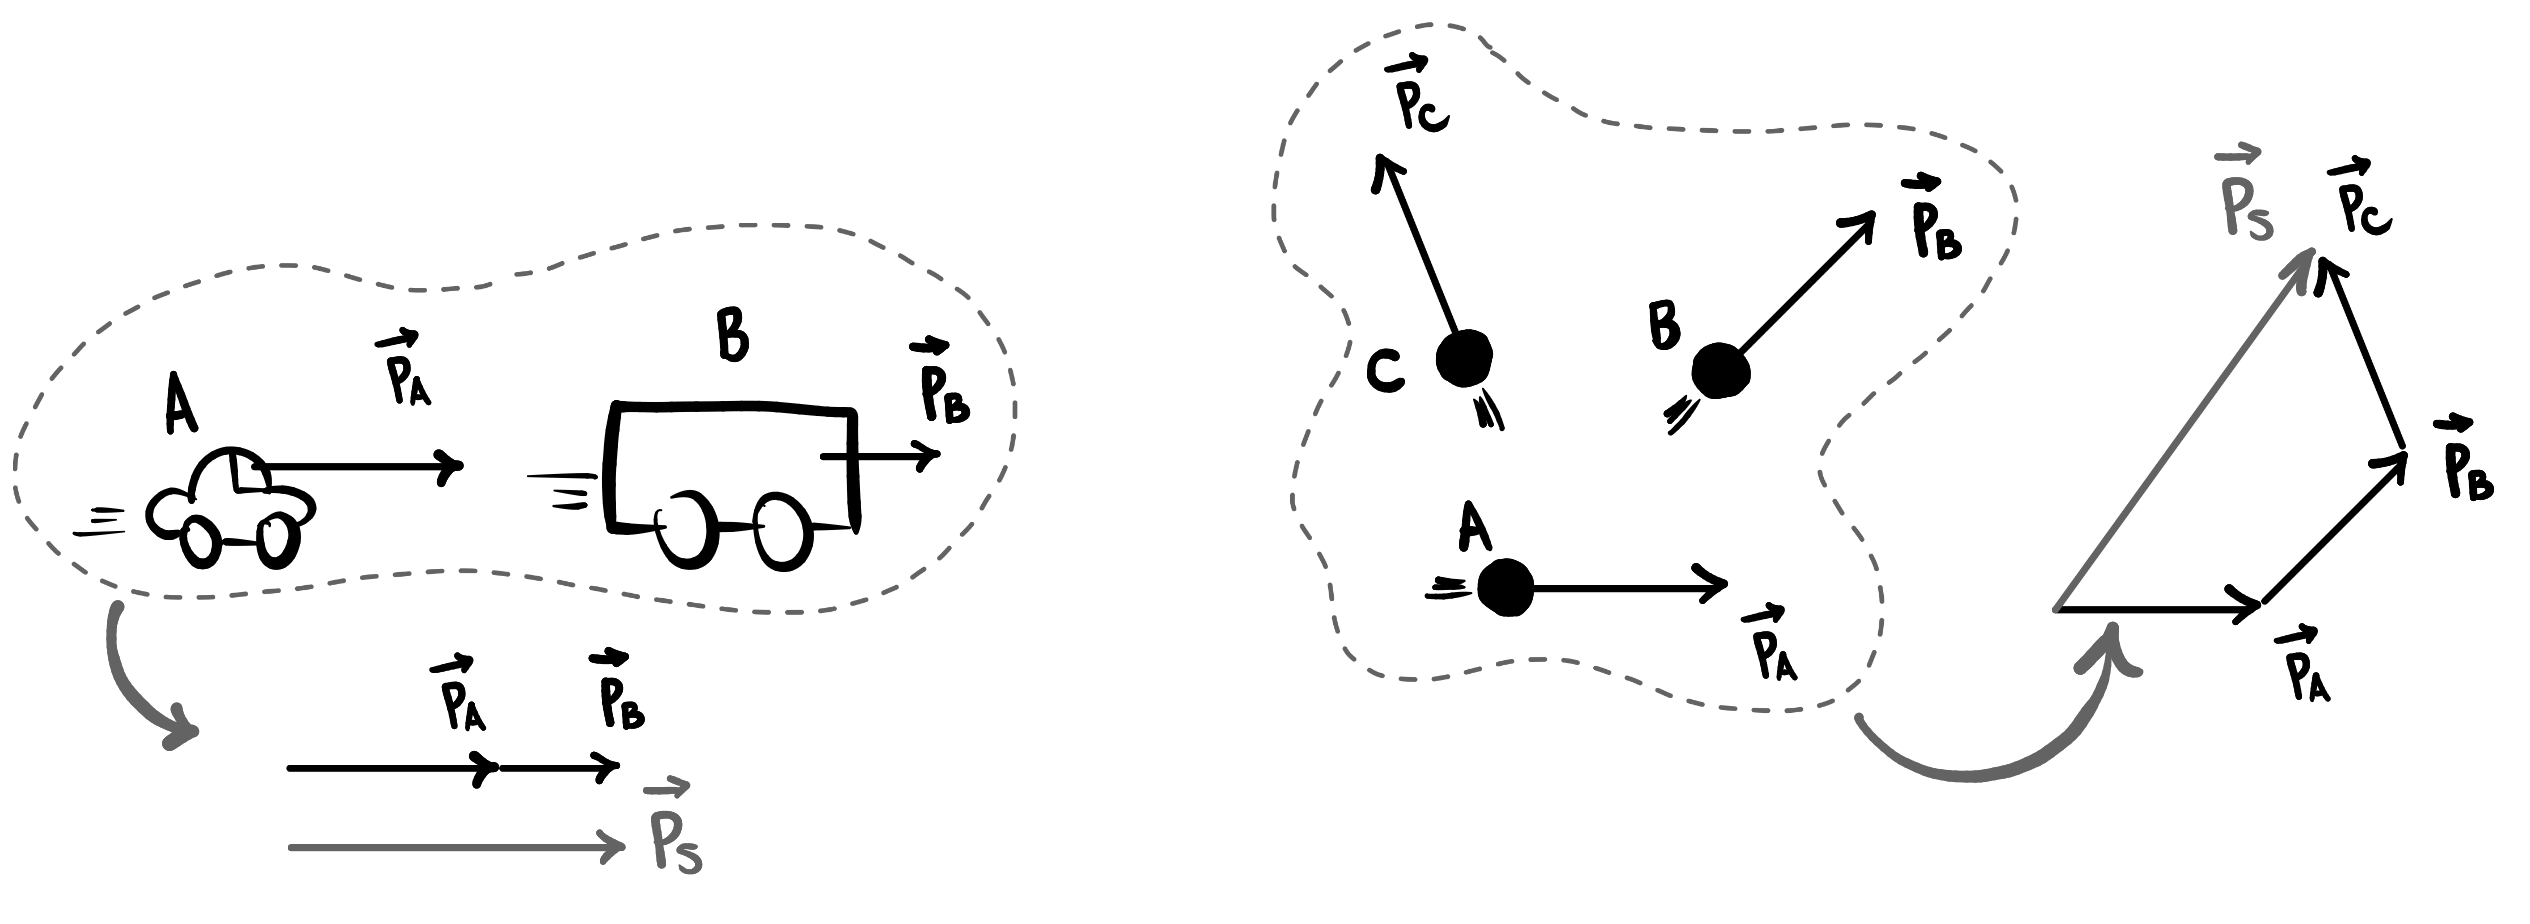
\includegraphics[width=0.9\linewidth]{imagensdinamicanewton/conservacaoqdm03.png}};
  \end{scope}
\end{tikzpicture}
\captionof{figure}{O momento linear total $\vec p_\text{s}$ de um sistema é uma grandeza vetorial obtida pela soma vetorial dos momentos lineares das partículas que compõem o sistema.}
\label{fig_newton_conservacaoqdm03}
} 
\vspace{0.3cm}

Vamos agora entender a razão pela qual a Equação \eqref{eq_newton_convervacaomomentolinear} é válida -- e qual é o seu significado físico. Considere a situação da Figura \ref{fig_newton_conservacaoqdm04}, que mostra duas partículas, $A$ e $B,$ que compõem o nosso sistema. Seus momentos inicialmente são $ p_{\text{A}}$ e $p_{\text{B}}$. As partículas colidem, trocando uma força $F$, que é a mesma em módulo e direção, apenas tendo o sentido oposto, como diz a Terceira Lei de Newton. A imagem do meio dessa figura destaca isso, representando o momento exato da colisão.

\vspace{0.3cm}
{
\centering
\begin{tikzpicture}
  \begin{scope}[blend mode=multiply]
    \node {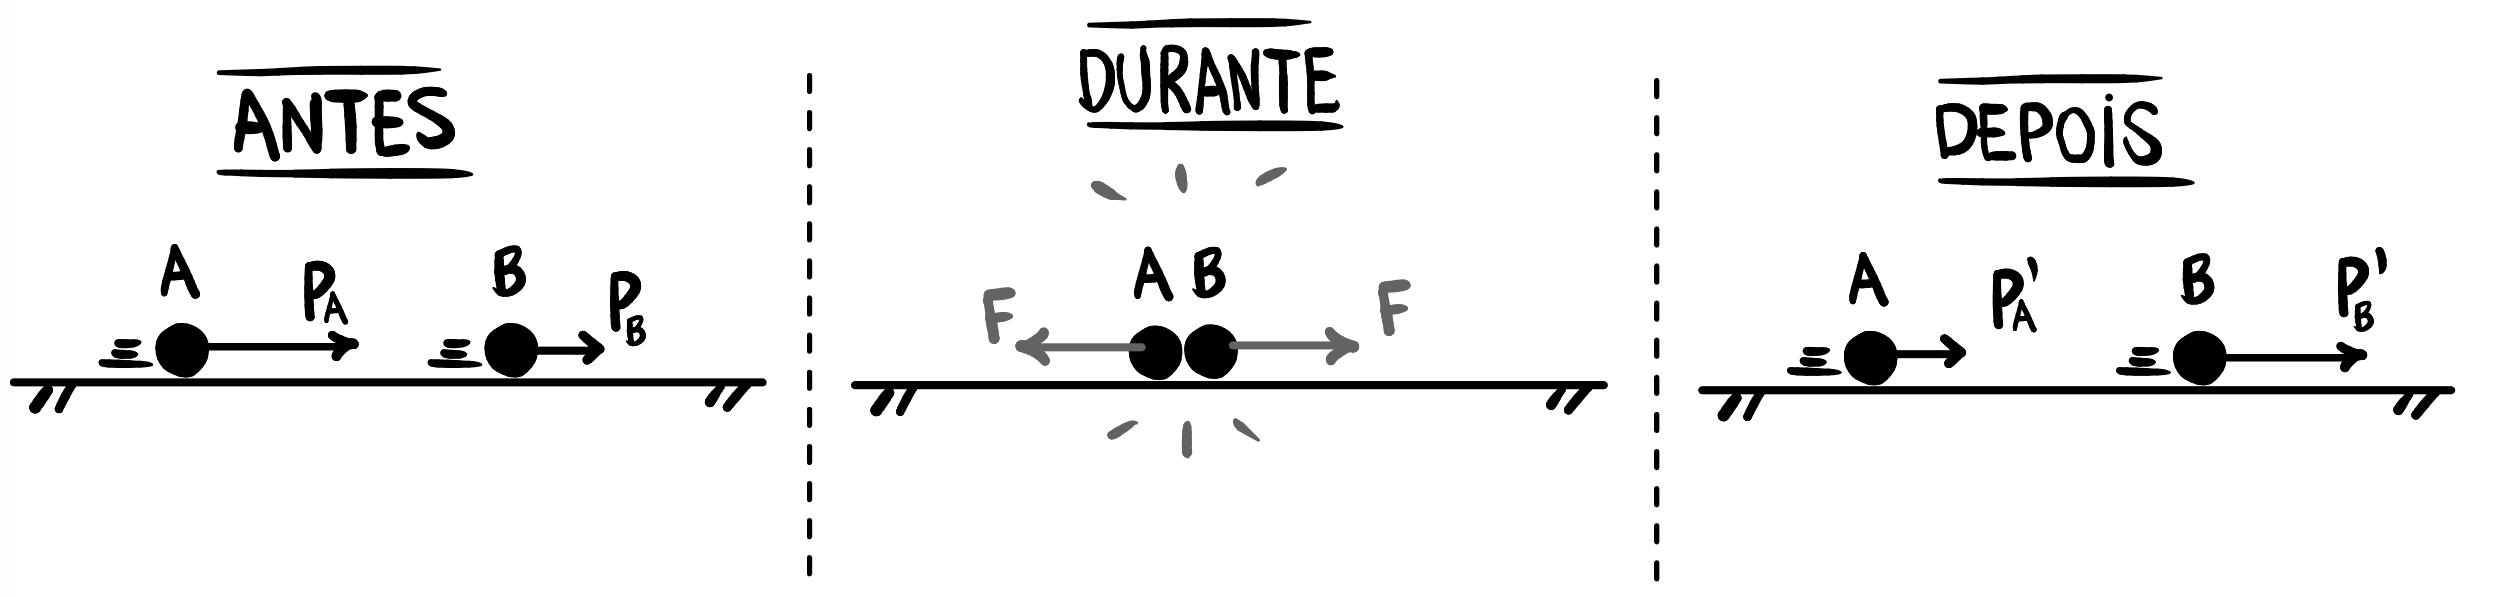
\includegraphics[width=0.9\linewidth]{imagensdinamicanewton/conservacaoqdm04.png}};
  \end{scope}
\end{tikzpicture}
\captionof{figure}{A colisão entre duas partículas $A$ e $B.$}
\label{fig_newton_conservacaoqdm04}
} 
\vspace{0.3cm}

Após o choque, os momentos finais das partículas são $ p_{\text{A}}'$ e $p_{\text{B}}'$. Note que, durante o choque, os impulsos trocados pelas partículas são iguais e opostos: elas trocam forças iguais durante o mesmo intervalo de tempo $\Delta t$ (tempo de duração do choque). Assim, sendo o impulso igual à variação do momento linear, como diz a Equação \eqref{eq_newton_teoremaimpulso}, o que a partícula $B$ ganha de momento linear é exatamente igual ao que a partícula $A$ perde, haja vista que elas trocam impulsos iguais e contrários.

\vspace{0.3cm}
{
\centering
\begin{tikzpicture}
  \begin{scope}[blend mode=multiply]
    \node {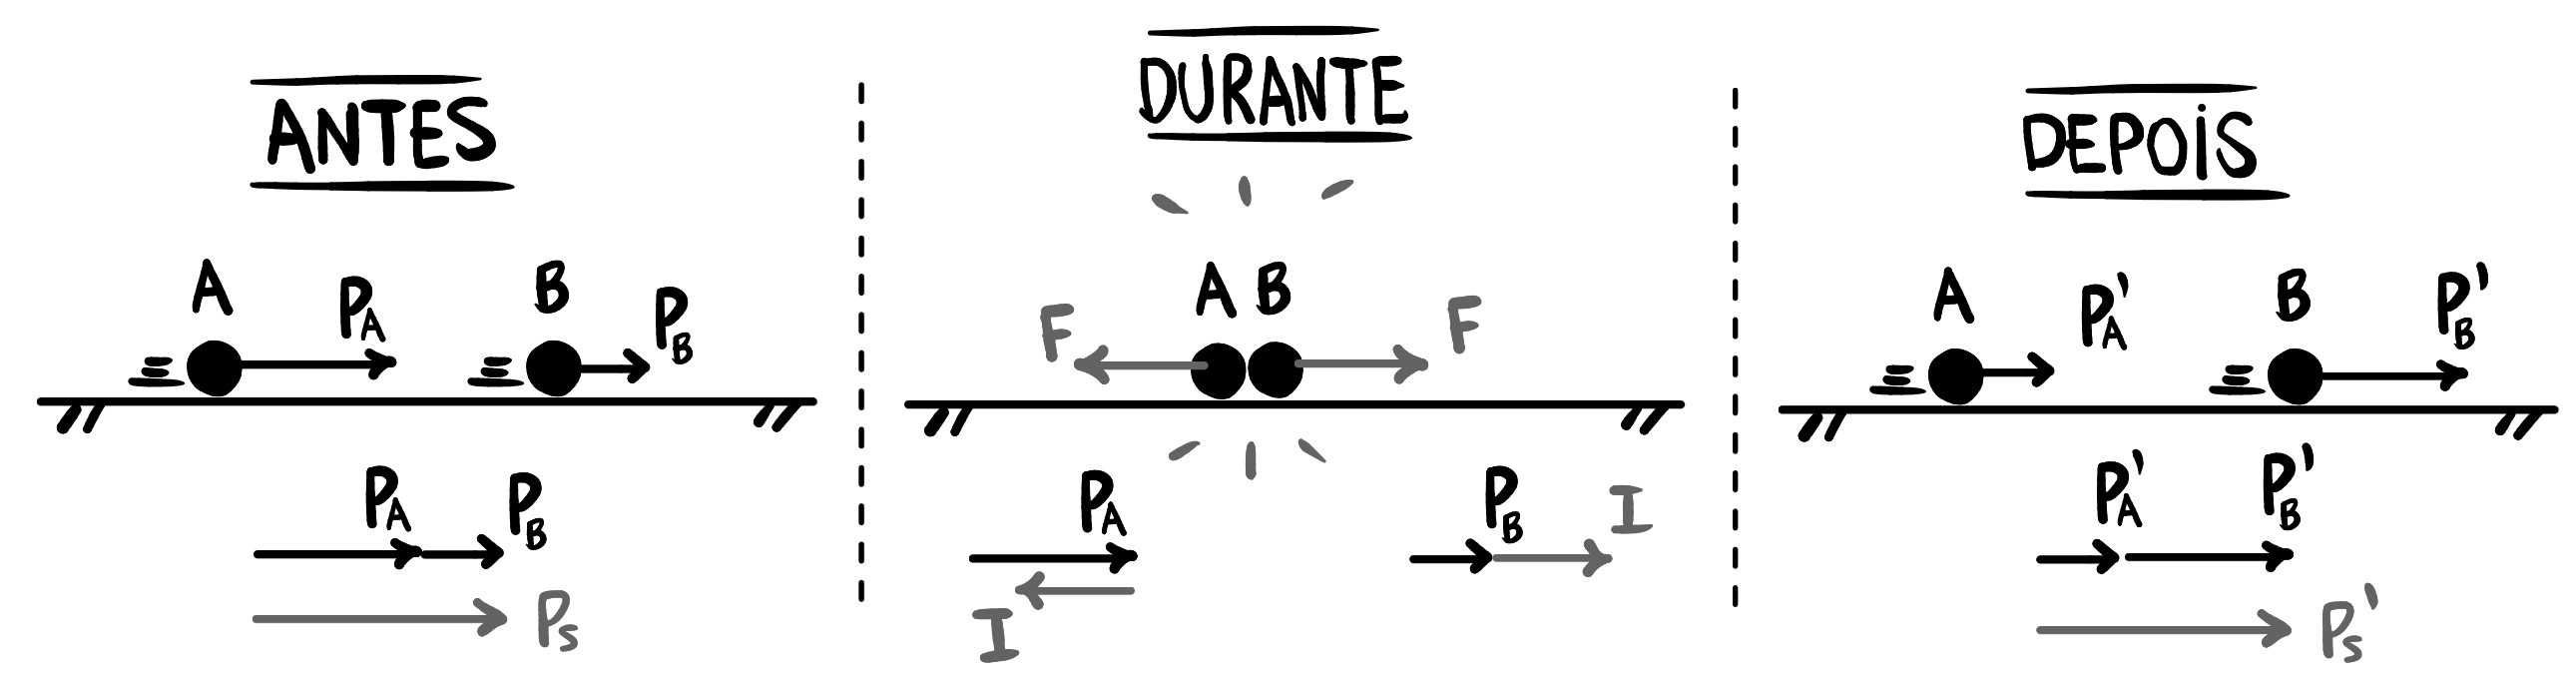
\includegraphics[width=0.9\linewidth]{imagensdinamicanewton/conservacaoqdm05.png}};
  \end{scope}
\end{tikzpicture}
\captionof{figure}{A lei de conservação do momento é uma consequência direta da Terceira Lei de Newton.}
\label{fig_newton_conservacaoqdm05}
} 
\vspace{0.3cm}

A Figura \ref{fig_newton_conservacaoqdm05} ilustra essa situação. Perceba que o efeito final é o de que o momento total do sistema ($A+B)$ ficou inalterado: a quantidade de momento que uma partícula ganha é exatamente igual ao que a outra partícula perde. Sendo assim, chegamos ao conteúdo da Equação \eqref{eq_newton_convervacaomomentolinear}: sob a ação de forças internas, o momento linear total de um sistema é conservado.

Note que isso é consequência direta da Terceira Lei de Newton: as forças, pela Terceira Lei de Newton, sempre virão aos pares. Sendo tais forças sempre internas ao sistema, tais pares estarão sempre dentro do sistema. Assim, toda força -- dentro do sistema -- terá uma outra igual e contrária, que gerará um impulso igual e contrário. Sendo o impulso total do sistema igual a zero, pela Equação \eqref{eq_newton_teoremaimpulso}, o momento não irá variar -- há apenas troca de momentos lineares pelas partículas internas ao sistema, mantendo constante o valor total do momento.

Para o leitor com maior afinidade analítica, podemos escrever isso de modo matemático. Considere o momento da colisão na situação da Figura \ref{fig_newton_conservacaoqdm05}. Durante o choque, as partículas trocam as forças $F$, que, vetorialmente, satisfazem, pela Terceira Lei de Newton, $\vec F_{\text{AB}} = - \vec F_{\text{BA}},$ e, se as partículas interagem por tal força ao longo de um tempo $\Delta t$, temos:

\begin{align}
    \vec F_{\text{AB}} &= - \vec F_{\text{BA}} \nonumber \\
    \vec F_{\text{AB}} \Delta t &= - \vec F_{\text{BA}}\Delta t \nonumber \\
    \vec I_{\text{AB}}  &= - \vec I_{\text{BA}} \nonumber \\
    \Delta \vec p_{\text{B}} &= -  \Delta \vec p_{\text{A}}, \nonumber
\end{align}

\noindent de onde conclui-se que o momento total do sistema não varia: $\Delta \vec p_{\text{S}}  =  \Delta (\vec p_{\text{A}}+\vec p_{\text{B}}) = \Delta \vec p_{\text{A}} + \Delta \vec p_{\text{B}} = 0. $

Note que, no desenvolvimento acima, usamos na terceira linha a definição de impulso, dada pela Equação \eqref{eq_newton_impulso}, além da Equação \eqref{eq_newton_teoremaimpulso} na linha seguinte, para dizer que o impulso que $B$ sente é igual à variação do seu momento linear, o mesmo valendo para $A.$ 

De forma ainda mais detalhada, logo após o choque os momentos das partículas $A$ e $B$ são

\begin{align}
    p_A'= p_A - F\Delta t \nonumber \\
    p_B'= p_B + F\Delta t \nonumber 
\end{align}

\noindent de modo que, ao somar as duas equações acima, teremos

$$ p_A' + p_B'  = p_A + p_B \implies \boxed{\Delta p_\text{SISTEMA} =0.} $$

\secgfe{Onde é usada}

Como já ficou claro no próprio contexto usado para construir a Equação \eqref{eq_newton_convervacaomomentolinear}: a conservação do momento linear será muito importante no estudo das colisões. 

% Isso porque, como mostra a Figura \ref{fig_newton_qdmcolisao001}, em que estuda-se o sistema composto pelas partículas $A$ e $B,$ ainda que hajam forças externas ao sistema, em uma colisão elas seram pouco relevantes.

Em uma análise rigorosa, o momento linear total de um sistema não é, em geral, conservado na presença de forças externas. De fato, a Segunda Lei de Newton aplicada ao sistema como um todo estabelece que a taxa de variação do momento linear total é igual à resultante das forças externas que atuam sobre ele. No entanto, ao estudarmos colisões, é comum afirmar que o momento linear total se conserva, independente das forças externas existirem ou não -- e essa afirmação, embora pareça contraditória à primeira vista, apoia-se em uma característica essencial desses fenômenos: a sua curta duração.

Uma colisão ocorre em um intervalo de tempo extremamente pequeno. Durante esse intervalo, as forças de interação entre os corpos envolvidos -- isto é, as forças internas ao sistema -- atingem valores muito elevados, sendo responsáveis por mudanças significativas nas velocidades das partículas. Em contraste, as forças externas, como o peso ou eventuais forças de atrito, mantêm intensidades comparativamente modestas e atuam ao longo do mesmo intervalo de tempo, que é muito curto.

Para compreender o efeito dessas forças sobre o momento linear, é fundamental considerar o conceito de impulso. A variação do momento linear de um sistema é dada pelo impulso da força resultante externa, isto é, pelo produto da força externa pelo intervalo de tempo durante o qual ela atua. Ainda que a força externa não seja nula, o tempo de duração da colisão é tão pequeno que o impulso associado a ela se torna desprezível quando comparado às trocas de momento promovidas pelas forças internas.

Assim, durante a colisão, as forças internas -- que ocorrem em pares de ação e reação, conforme a Terceira Lei de Newton -- produzem variações de momento iguais e opostas entre os corpos, cancelando-se mutuamente quando se considera o sistema como um todo. Já as forças externas, embora presentes, não têm tempo suficiente para provocar uma variação significativa no momento total.

\vspace{0.3cm}
{
\centering
\begin{tikzpicture}
  \begin{scope}[blend mode=multiply]
    \node {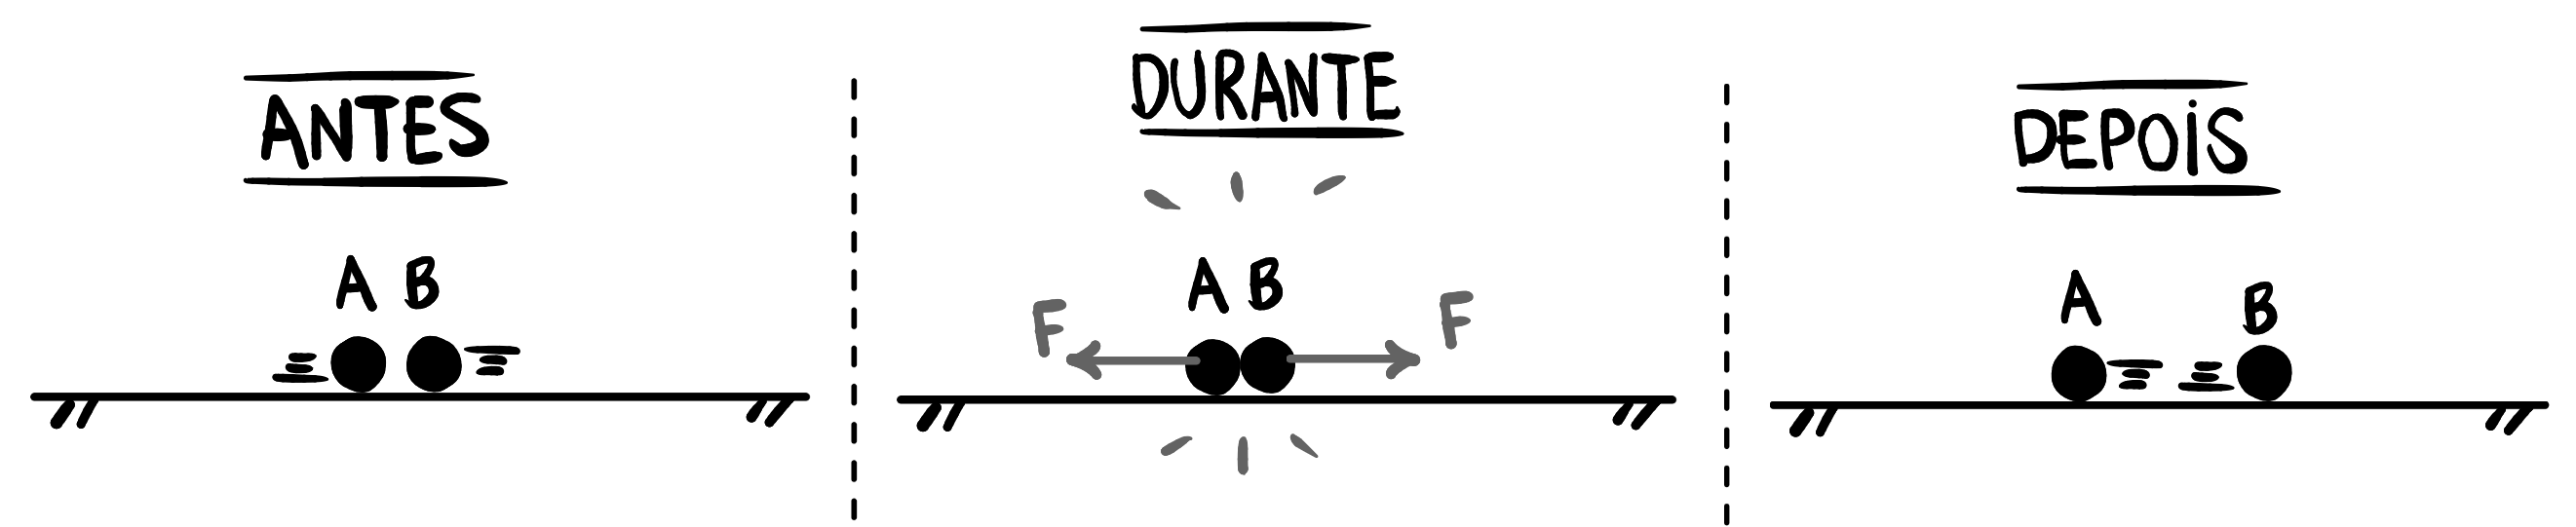
\includegraphics[width=0.8\linewidth]{imagensdinamicanewton/qdmcolisao001.png}};
  \end{scope}
\end{tikzpicture}
\captionof{figure}{Situação logo antes, durante e logo depois da colisão.}
\label{fig_newton_qdmcolisao001o}
} 
\vspace{0.3cm}


Dessa forma, pode-se concluir que, entre os instantes imediatamente anterior e imediatamente posterior à colisão, como ilustra a Figura \ref{fig_newton_conservacaoqdm05}, o momento linear total do sistema permanece praticamente constante.\footnote{Note que trata-se, portanto, de uma conservação aproximada, cuja validade decorre do fato de que o impulso das forças externas, durante o breve intervalo da colisão, é desprezível diante das intensas interações internas.} Assim, em qualquer tipo de colisão o momento linear -- imediatamente antes do choque e imediatamente após o choque -- será conservado, e este será um fato extremamente importante para estudarmos colisões.





Considere, por exemplo, a situação da Figura \ref{fig_newton_qdmcolisao001}, que trata da colisão de dois corpos $A$ e $B$, que se movem em um solo horizontal sem atrito. Fornecem-nos a velocidade de um deles após a colisão, e pede-se a velocidade do outro.

\vspace{0.3cm}
{
\centering
\begin{tikzpicture}
  \begin{scope}[blend mode=multiply]
    \node {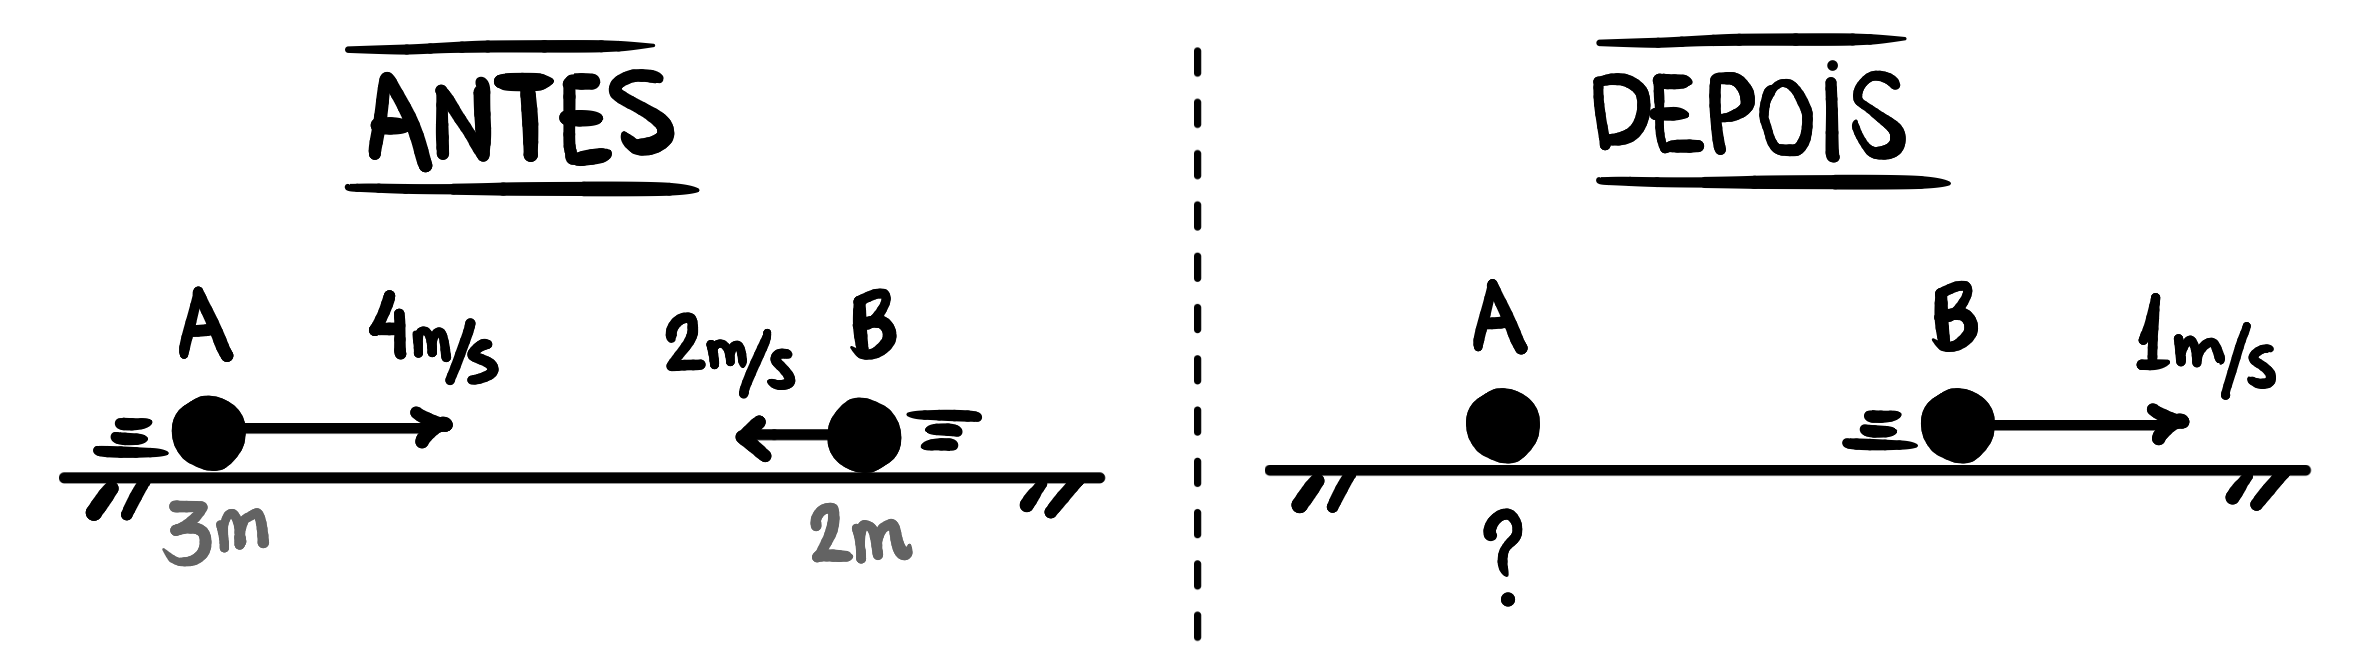
\includegraphics[width=0.6\linewidth]{imagensdinamicanewton/qdmcolisao01.png}};
  \end{scope}
\end{tikzpicture}
\captionof{figure}{Colisão entre duas partículas $A$ e $B$.}
\label{fig_newton_qdmcolisao001}
} 
\vspace{0.3cm}

Sabemos que imediatamente antes da colisão e imediatamente após ela o momento linear total do sistema é conservado, e podemos resolver o problema usando a Equação \eqref{eq_newton_convervacaomomentolinear}. O momento linear total do sistema logo antes da colisão é

$$ p_0 = m_Av_A + m_Bv_B = 3m \cdot 4 - 2m\cdot 2 = 8m, $$

\noindent em que arbitramos o sentido para a direita como sendo positivo. Após a colisão, o momento linear total do sistema é 

$$ p_f = m_Av_A' + m_Bv_B' = 3mv_A' + 2m \cdot 1 = m(3v_A'+2). $$

Usando a Equação \eqref{eq_newton_convervacaomomentolinear}, teremos que

$$ p_0 = p_f \implies 8 \cancel m =  \cancel m(3v_A'+2)\implies \boxed{v_A'= 3 \text{ m/s} ,}$$

\noindent e, como a velocidade saiu com sinal positivo, isso quer dizer que a bolinha $A$ se move, após o choque, para a direita, com velocidade de $3$ m/s.


\secgfe{Erros comuns}

Um erro bastante comum é o estudante confundir forças internas com forças externas. Sendo assim, certifique-se de ter compreendido bem a diferença entre as duas. Na seção seguinte, sobre \textbf{Observações}, trabalharemos com ainda mais detalhes essas diferenças.

Outro erro comum é não se atentar ao caráter vetorial da Equação \eqref{eq_newton_convervacaomomentolinear}. Tal equação diz respeito à conservação do momento linear, que é uma grandeza vetorial. Assim, tal como fazíamos com forças, é comum decompor o movimento em duas direções ortogonais independentes. Assim, ao analisar o movimento em $y$ e em $x$, podemos constatar que existem forças externas em $y$, de modo que o momento linear naquela direção não se conserva; contudo, podem não haver forças externas em $x$, de modo que o momento linear nessa direção se conservaria. Isto é, matematicamente, teríamos:

$$ \vec p \text{ não se conserva} \begin{cases}
      \vec p_\text{x} \text{ se conserva}   \\
      \vec p_\text{y} \text{ não se conserva}   \\
\end{cases}$$

Ou seja, o momento linear como um todo não se conserva (já que uma das suas componentes, a vertical, varia); porém, o momento linear em uma certa direção é conservado. Considere, por exemplo, a situação da Figura \ref{fig_newton_qdmsistemaisolado01}. Ela mostra uma pequena esfera de massa $m$, lançada horizontalmente para cair na caçapa do carrinho de massa $M,$ que se encontra inicialmente em repouso.

Note que, sendo o sistema as massas $m$ e $M$, existem forças externas atuando, como a normal e o peso. Contudo, essas forças externas compartilham a característica de serem todas verticais. Logo, analisando as direções perpendiculares de forma independente, conclui-se que o momento linear na vertical \textbf{não é conservado,} haja vista que a força peso gera um impulso externo, que faz a massa $m$ ganhar momento linear na vertical, como mostram as imagens da Figura \ref{fig_newton_qdmsistemaisolado01}.

\vspace{0.3cm}
{
\centering
\begin{tikzpicture}
  \begin{scope}[blend mode=multiply]
    \node {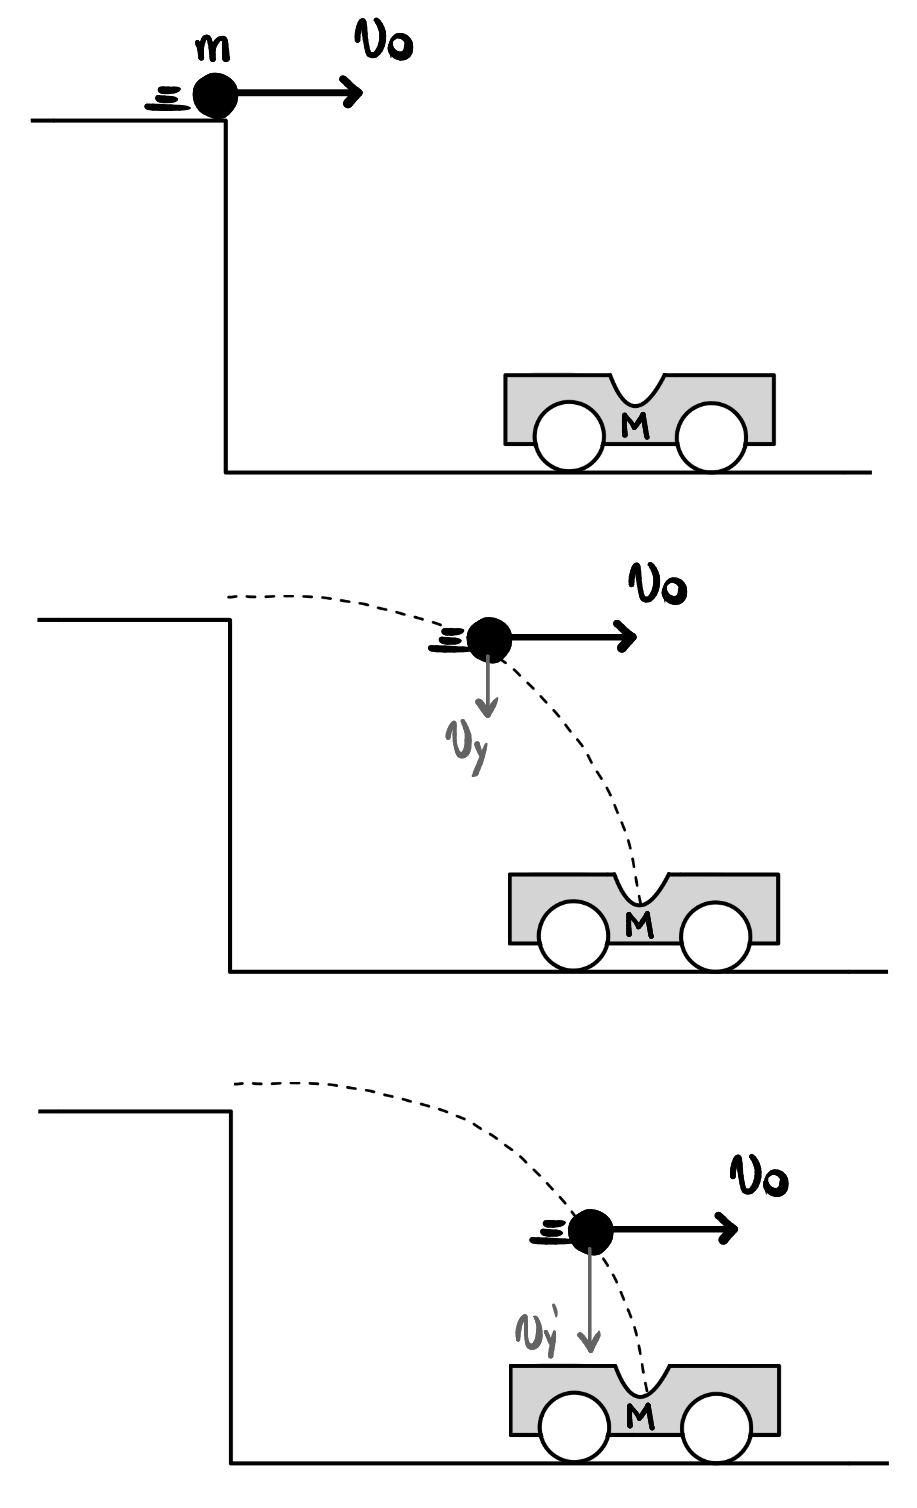
\includegraphics[width=0.35\linewidth]{imagensdinamicanewton/sistemaisoladohorizontal2.png}};
  \end{scope}
\end{tikzpicture}
\captionof{figure}{O sistema composto pelas massas $m$ e $M$ é isolado de forças externas na horizontal.}
\label{fig_newton_qdmsistemaisolado01}
} 
\vspace{0.3cm}


Contudo, na horizontal não existe nenhuma força externa (estamos desprezando a resistência do ar), de modo que, ao longo da queda da bolinha, a velocidade (e, portanto, o momento) horizontal sempre se mantém constante. Quando a bolinha cai na caçapa do carrinho de massa $M$, perceba que ela irá ``empurrar'' o carrinho para a frente com uma força $F$, porém o carrinho, reagindo, empurra a bolinha para trás com uma força de mesma intensidade. Ou seja, as forças horizontais que surgem são internas ao sistema: a bolinha injetará momento linear no carrinho, exatamente o mesmo tanto de momento linear que ela perderá. 


\vspace{0.3cm}
{
\centering
\begin{tikzpicture}
  \begin{scope}[blend mode=multiply]
    \node {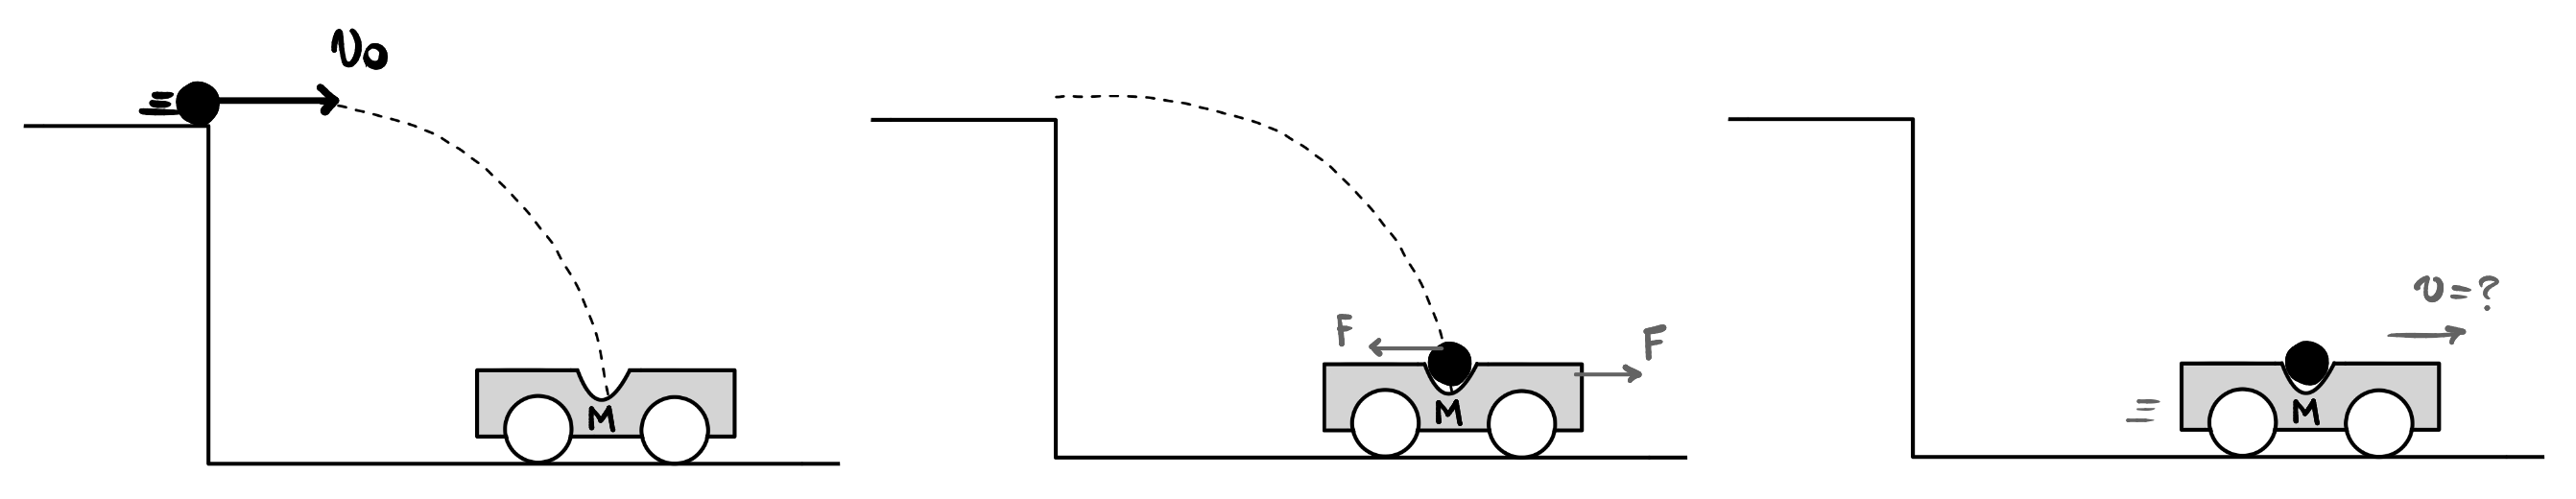
\includegraphics[width=1.0\linewidth]{imagensdinamicanewton/sistemaisoladohorizontal1.png}};
  \end{scope}
\end{tikzpicture}
\captionof{figure}{O momento linear do sistema se conserva na horizontal, uma vez que as forças externas atuam apenas na vertical.}
\label{fig_newton_qdmsistemaisolado02}
} 
\vspace{0.3cm}



A Figura \ref{fig_newton_qdmsistemaisolado02} ilustra essa situação, mostrando as situações antes da colisão, durante a colisão e após a colisão. Assim, equacionando a conservação do momento linear na horizontal antes e após a colisão, teremos:

$$ p_{0x} = p_{fx} \implies mv_0 = mv + Mv \implies \boxed{v = \dfrac{mv_0}{(m+M)}.}$$

Ou seja, partindo da premissa de que a bolinha ``gruda'' na caçapa do carrinho e passa a se mover horizontalmente junto dele, os dois compartilharão da mesma velocidade $v$, de modo que o momento linear do sistema na horizontal após a colisão é $mv+Mv.$ Assim, sabendo os valores das massas e da velocidade inicial da bolinha, a expressão acima nos permitiria encontrar o valor da velocidade $v$ com que o sistema bolinha + carrinho se moveria após o choque.

Perceba que, ainda que haja forças externas (o peso, neste caso), foi possível desenvolver o problema usando a conservação do momento linear, uma vez que notamos haver uma direção em que o sistema estava isolado, de modo que poderíamos usar a conservação de $\vec p$ naquela direção.


\secgfe{Observações}

Faremos aqui uma breve releitura da Segunda Lei de Newton, tópico que pode ser pulado em uma primeira leitura.

Como diz a Equação \eqref{eq_newton_teoremaimpulso}, sabemos que $ \vec I =\Delta \vec p$, e, pela definição de impulso, isso se escreve como $\vec F_\text{R} \Delta t = \Delta \vec p,$ o que pode ser escrito como

\begin{equation}
    \vec F_{\text{R}} = \dfrac{\Delta \vec p}{\Delta t},
    \label{eq_newton_forcavariamomento}
\end{equation}


\noindent ou seja, a força resultante $\vec F_{\text{R}}$ é responsável por variar o momento linear de uma partícula. Perceba que a relação acima é simplesmente a Segunda Lei de Newton, porém escrita em termos do momento linear. Caso façamos $\vec p = m \vec v$, seremos levados a

$$  \vec F_{\text{R}} = \dfrac{\Delta   \vec p}{\Delta t} = \dfrac{\Delta  (m \vec v)}{\Delta t} = m  \dfrac{\Delta \vec v}{\Delta t} = m \vec a,$$

\noindent como se esperava.

Considere agora um sistema de $N$ partículas, cujos momentos são $\vec p_{1}, \vec p_{2}, \vec p_{3}, \dots ,\vec p_{N}$. Considere que o sistema está isolado de forças externas, ou seja, as únicas forças que atuam no sistema são de interações entre elas. Logo, para cada força $\vec F_{\text{KJ}}$ que a partícula $K$ exerce sob a partícula $J$, existe sua reação $\vec F_{\text{JK}}= -\vec F_{\text{KJ}}$, que é a força feita por $J$ em $K.$

Escrevendo a Equação \eqref{eq_newton_teoremaimpulso} para cada uma das partículas, teríamos as equações\footnote{Perceba que o tempo de interação entre a partícula $A$ e a partícula $B$ é, necessariamente, o mesmo tempo de interação entre a partícula $B$ e a partícula $A$, por se tratar, essencialmente, da mesma interação. Logo, o intervalo de tempo $\Delta t$ nas duas primeiras equações em \eqref{eq_newton_desenvolvimentoconservacao} deve certamente ser o mesmo. Contudo, o intervalo de tempo da terceira linha não precisa ser o mesmo que aquele das duas primeiras; precisaria ser o mesmo apenas do intervalo de tempo da quarta linha, uma vez que trata-se da mesma interação: de $C$ com $D.$ De todo modo, como veremos, tais intervalos de tempo estarão sempre multiplicados por zero, de modo que serão pouco relevantes para a nossa análise.}



\begin{equation}
\begin{aligned}
\vec{I}_1 &= \vec{F}_{AB}\Delta t = \Delta \vec{p}_1 \nonumber \\
\vec{I}_2 &= \vec{F}_{BA}\Delta t = \Delta \vec{p}_2 \nonumber \\
\vec{I}_3 &= \vec{F}_{CD}\Delta t = \Delta \vec{p}_3 \nonumber \\
\vec{I}_4 &= \vec{F}_{DC}\Delta t = \Delta \vec{p}_4 \nonumber\\
          &\vdots \nonumber \\
\vec{I}_{(N-1)} &= \vec{F}_{PQ}\Delta t = \Delta \vec{p}_{(N-1)} \nonumber\\
\vec{I}_N &= \vec{F}_{QP}\Delta t = \Delta \vec{p}_N \nonumber
\end{aligned}
\label{eq_newton_desenvolvimentoconservacao}
\end{equation}


Somando todas elas, teremos:\footnote{Teríamos, na verdade, vários pares a mais a serem formados, como, por exemplo, da força $\vec F_{\text{AC}}$ de interação entre $A$ e $C$, ou da força $\vec F_{\text{DN}}$, da interação entre a partícula $D$ e a partícula $N$. Contudo, cada uma dessas possuiria um elemento inverso associado dentro do sistema, isto é, ter-se-ia a força $\vec F_{\text{CA}} = - \vec F_{\text{AC}}$, que seria a força de $C$ em $A$; e também a força $\vec F_{\text{ND}} = - \vec F_{\text{DN}}$, feita pela partícula $N$ sob a partícula $D$. Sendo assim, ao somar todas as equações essas forças sempre se cancelariam duas a duas, como ocorreu na versão simplificada que fizemos.}

\begin{align}
     \Delta (\vec p_1 + \vec p_2 +  \dots +\vec p_M + \vec p_N) &= \underbrace{(\vec F_{\text{AB}} + \vec F_{\text{BA}})}_{\text{zero}}  \Delta t + \underbrace{(\vec F_{\text{CD}} + \vec F_{\text{DC}})}_{\text{zero}} \Delta t+ \dots + \underbrace{(\vec F_{\text{PQ}} + \vec F_{\text{QP}})}_{\text{zero}} \Delta t \nonumber \\
     &= 0. \nonumber
\end{align}


Essa seria uma outra forma de mostrarmos a validade da Equação \eqref{eq_newton_convervacaomomentolinear}. Contudo, queremos nos ater a um outro aspecto. Perceba que do lado esquerdo da equação acima temos a variação total de momento do sistema, isto é, temos $\Delta \vec p_{\text{SISTEMA}} =  \Delta \vec p_1 +  \Delta \vec p_2 + \dots +  \Delta \vec p_N,$ enquanto que do lado direito temos a resultante das forças atuando sob o sistema, que, sendo apenas forças internas, se anulam duas a duas, resultando em zero, que é a condição que garante a conservação do momento linear do sistema.

Contudo, caso houvesse também forças externas atuando no sistema, essas não se anulariam -- uma vez que sua reação estaria em uma partícula fora do sistema, o que não entraria na soma das forças sob partículas pertencentes ao sistema. Logo, do lado direito da equação sobraria, ao invés de zero, o somatório das forças externas que atuam no sistema. De forma matemática, caso o leitor prefira, teríamos.

\begin{equation}
    \sum \vec F_{\text{EXTERNAS}} = \dfrac{\Delta \vec p_{\text{SISTEMA}}}{\Delta t} .
    \label{eq_newton_segundaleisistemaparticulas}
\end{equation}

Essa seria uma certa adaptação da Segunda Lei de Newton aplicada a sistemas de partículas: o somatório das forças externas ao sistema é responsável por variar o momento linear do sistema. Naturalmente, se tivermos $ \sum \vec F_{\text{EXTERNAS}} = 0,$ teríamos um sistema isolado, e a Equação \eqref{eq_newton_segundaleisistemaparticulas} se reduziria para a Equação \eqref{eq_newton_convervacaomomentolinear}: a lei de conservação do momento linear.

Considere, por exemplo, as duas situações dos patinadores de rua da Figura \ref{fig_newton_qdmpatins}. Do lado esquerdo temos um indivíduo que empurra a parede com uma certa força $F$ e, pela Terceira Lei de Newton, toma uma força $F$ da parede, para a esquerda. Sendo o menino sob os patins o nosso sistema, a força $F$ em questão é uma \textbf{força externa ao sistema}, de modo que, pela Equação \eqref{eq_newton_segundaleisistemaparticulas}, o momento linear do sistema (menino sob os patins) irá variar: ele ganha momento para a esquerda, justamente por conta do impulso gerado pela força $F$ feita sob ele pela parede. 

\vspace{0.3cm}
{
\centering
\begin{tikzpicture}
  \begin{scope}[blend mode=multiply]
    \node {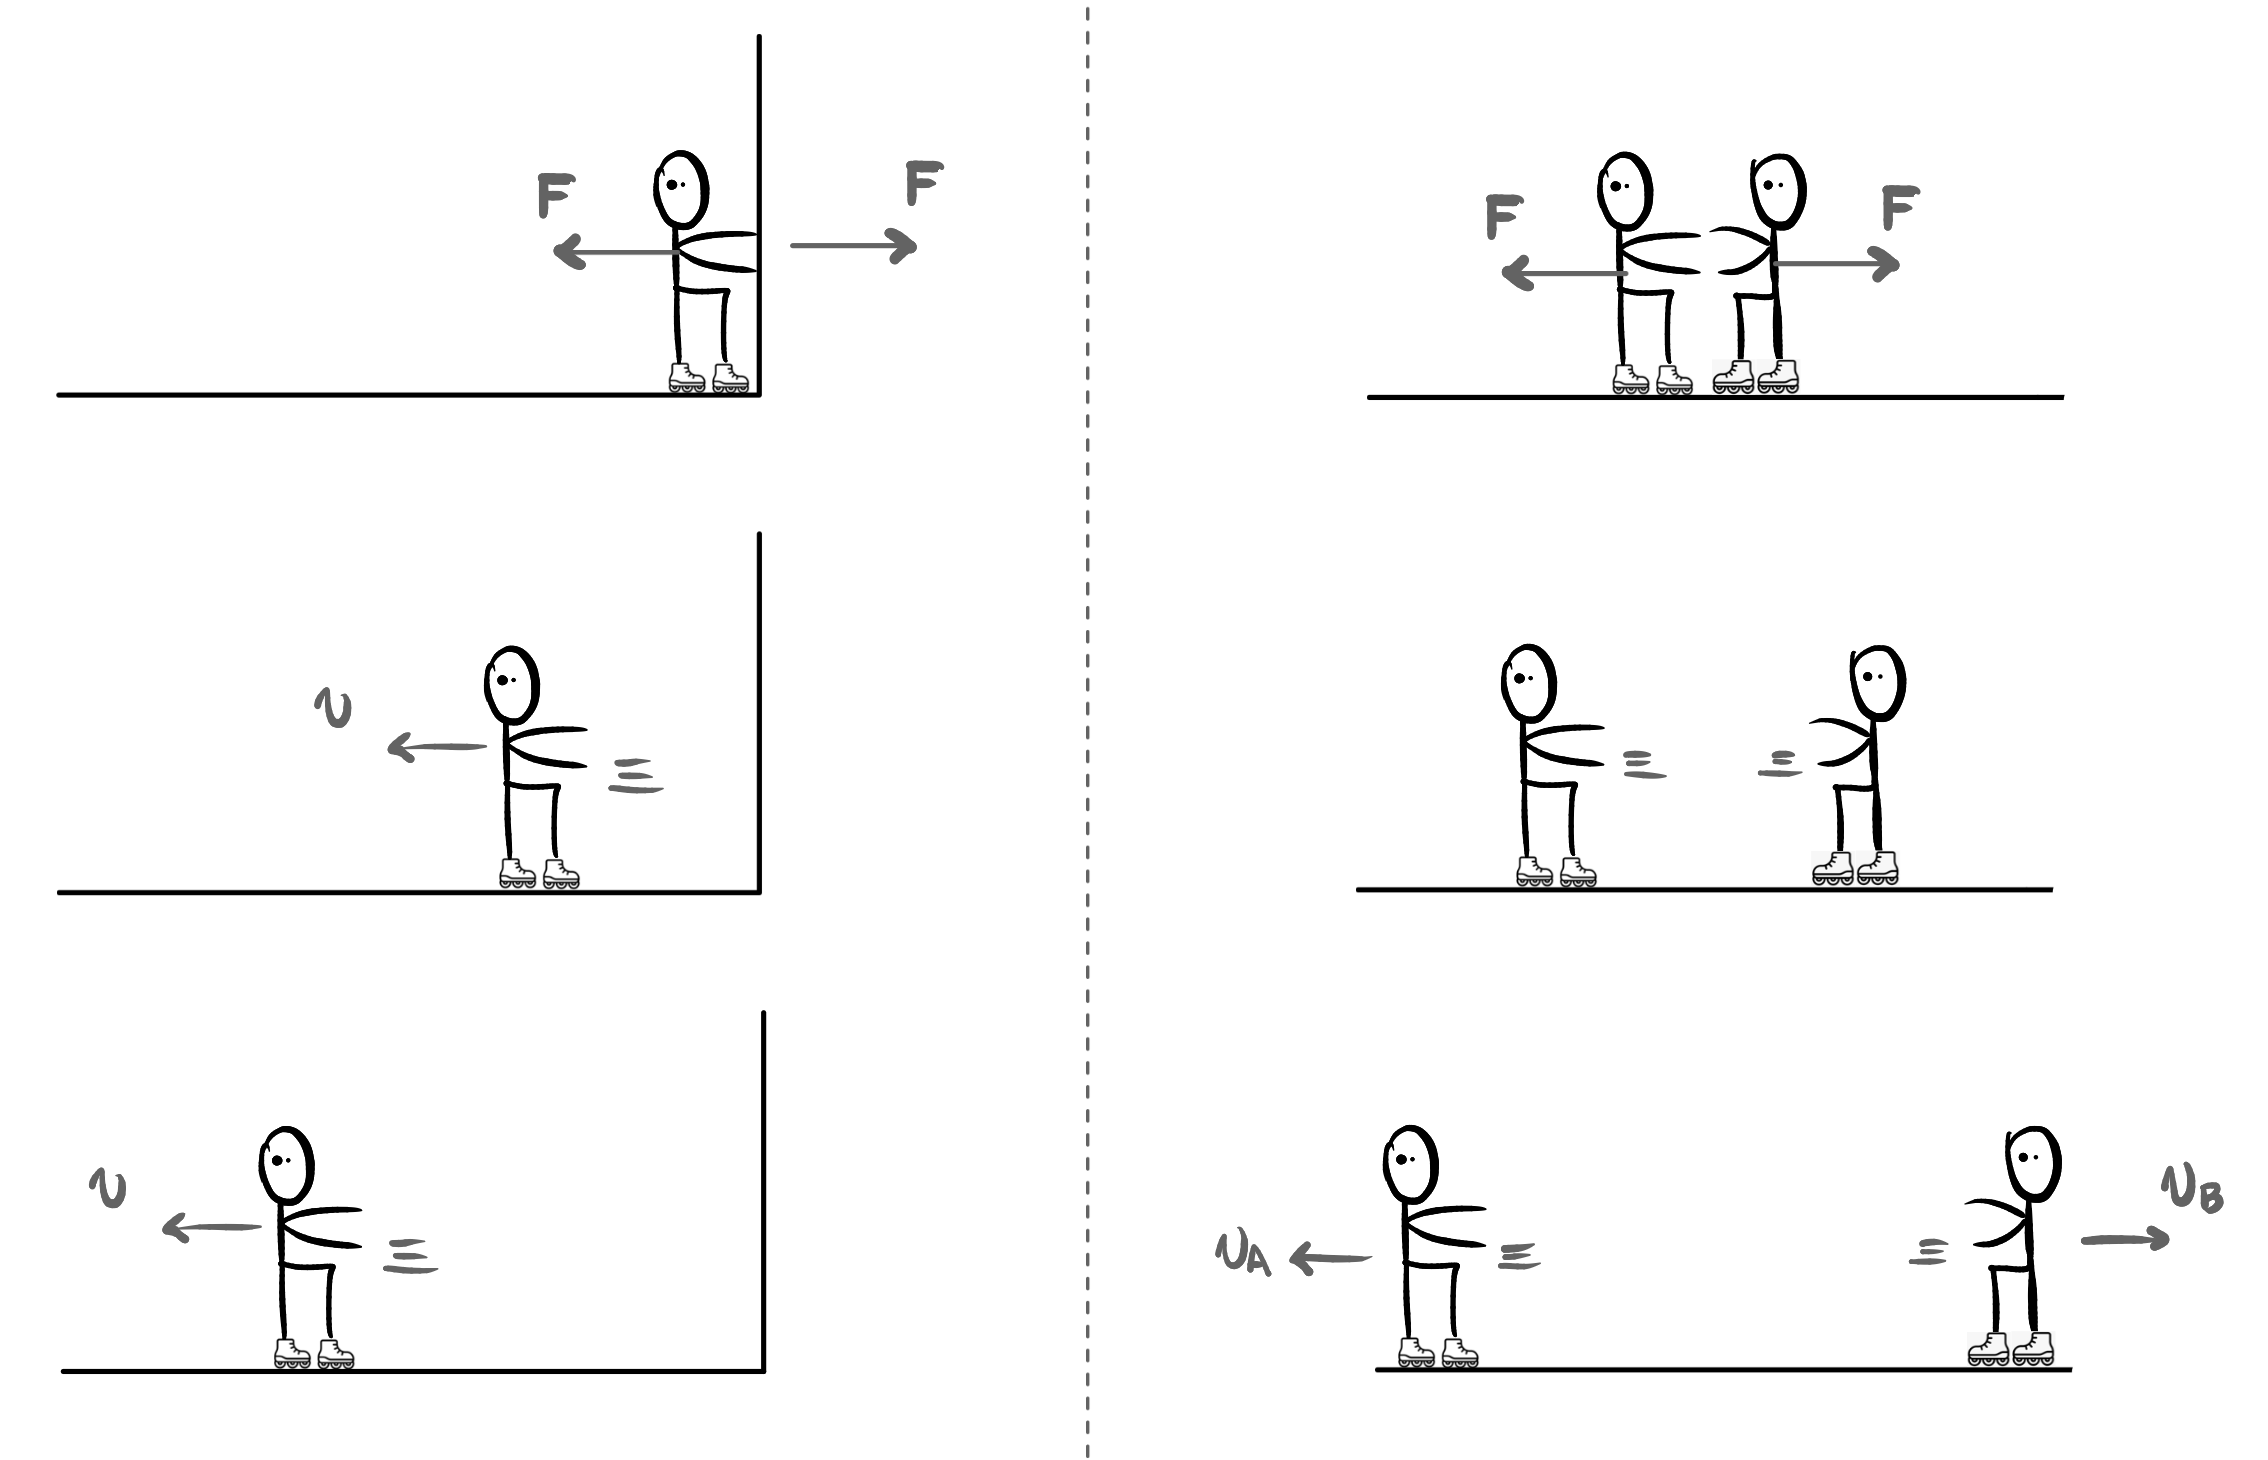
\includegraphics[width=0.8\linewidth]{imagensdinamicanewton/conservacaoqdmpatins.png}};
  \end{scope}
\end{tikzpicture}
\captionof{figure}{Sistema não isolado vs sistema isolado.}
\label{fig_newton_qdmpatins}
} 
\vspace{0.3cm}

Já no lado direito da figura temos uma situação com dois indivíduos, digamos $A$ e $B,$ parados sob os seus patins. O indivíduo $A$, então, empurra o indivíduo $B$ com uma força $F$. Pela Terceira Lei de Newton, $B$ faz uma força igual e contrária em $A$. Sendo o sistema formado pelos indivíduos $A$ e $B$, esse par de forças é interno ao sistema, de modo que, pela Equação \eqref{eq_newton_segundaleisistemaparticulas}, sem ação de forças externas, o momento linear do sistema deve ser conservado. 

Assim, um indivíduo se move para um lado com exatamente o mesmo momento que o outro indivíduo adquire para o outro, de modo a manter o momento linear do sistema igual a zero. Poderíamos, caso quiséssemos, computar inclusive a relação que tais velocidades devem satisfazer, exigindo que o momento linear total se conserve:

$$ p_0 = p_f \implies 0 = m_Av_A + m_Bv_B \implies v_B = -\dfrac{m_A}{m_B} v_A,$$

\noindent em que o sinal negativo indica que $v_B$ possui sentido contrário ao de $v_A,$ como esperado. Assim, sabendo as massas dos indivíduos e uma das velocidades, seria possível determinar a outra.

Note, portanto, que na situação à esquerda da Figura \ref{fig_newton_qdmpatins} o momento linear do sistema varia: ele era zero e passa a adquirir um valor não nulo, apontando para a esquerda. Isso se dá porque forças externas atuaram no sistema -- a força feita pela parede (agente externo) no menino.

Já na situação da direita, o momento linear do sistema não varia: apesar de os indivíduos $A$ e $B,$ que compõem o sistema, adquirirem velocidades, isso se dá de tal modo que o momento que um adquire é igual e contrário ao que o outro adquire, o que faz o momento linear total do sistema continuar sendo nulo, uma vez que trata-se de uma grandeza vetorial. Assim, a Equação \eqref{eq_newton_convervacaomomentolinear} é satisfeita, como esperado, uma vez que apenas forças internas atuaram em tal sistema.



\vspace{0.3cm}


\begin{exemplo}[Nível I]\label{exemplo_newton_conservacaomomentolinearex01}

Duas bolinhas de massa $m_A=1$ kg e $m_B =5$ kg se encontram dispostas como na Figura \ref{fig_newton_qdmcolisao001o} (p. \pageref{fig_newton_qdmcolisao001o}). As duas, contudo, se movem inicialmente para a direita, com velocidades $v_A = 5$ m/s e $v_B = 1$ m/s.

Após a colisão, a bolinha $B$ se move com velocidade de $3$ m/s para a direita. Qual é a velocidade da segunda bolinha após o choque?

\resolucao

Convencionado que o sentido positivo é para a direita, teremos, para o momento linear total antes do choque:

$$ p_0 = m_Av_A + m_Bv_B = 1 \cdot 5 + 5 \cdot 1 = 10 \text{ kg m/s}.$$

Para o momento linear do sistema após o choque teremos

$$  p_f = m_Av_A' + m_Bv_B' = 1 \cdot v_A'+ 5 \cdot 3 = (v_A'+ 15). $$

Da conservação do momento linear do sistema, segue que $p_0 = p_f$, ou seja:

$$ v_A'+ 15 = 10 \implies  \boxed{v_A' = -5 \text{m/s} ,}$$

\noindent em que o sinal negativo quer dizer que a bolinha $A$ recua para a esquerda após o choque.

\end{exemplo}


\vspace{0.3cm}


\begin{exemplo}[Nível II]\label{exemplo_newton_conservacaomomentolinearex02}

Duas partículas de mesma massa sofrem uma colisão. Inicialmente uma delas se move com velocidade $v,$ enquanto a outra está parada.

{
\centering
\begin{tikzpicture}
  \begin{scope}[blend mode=multiply]
    \node {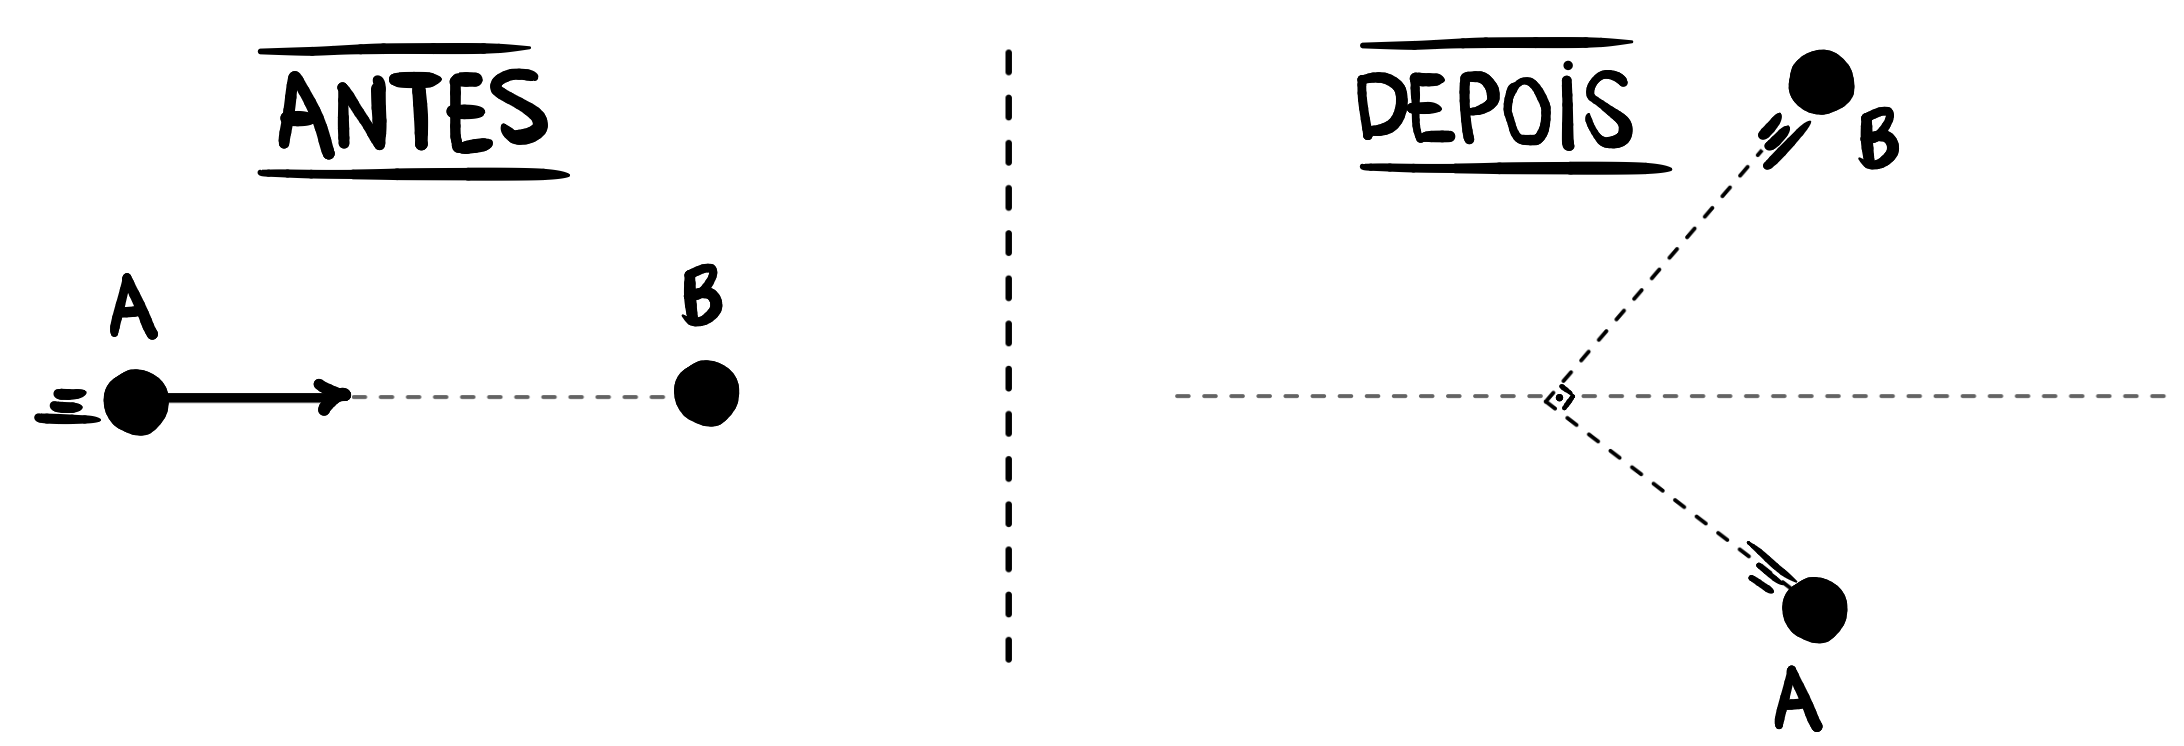
\includegraphics[width=0.6\linewidth]{imagensdinamicanewton/colisao2dqdm1.png}};
  \end{scope}
\end{tikzpicture}
\captionof{figure}{Colisão bidimensional entre duas partículas $A$ e $B$.}
\label{fig_newton_qdmcolisao2d01}
} 
\vspace{0.3cm}

Após o choque as duas partículas saem em direções distintas, como mostra a Figura \ref{fig_newton_qdmcolisao2d01}. Encontre a velocidade da partícula $B,$ sabendo que a velocidade da partícula $A$ após o choque é $\sfrac{v\sqrt 3}{2}.$

\resolucao

Temos agora um problema bidimensional, de modo que não será possível tratar as velocidades (e momentos lineares) como escalares, apenas atribuindo sinais distintos para direções distintas. Podemos decompor as velocidades nas direções vertical, $y,$ e horizontal, $x,$ e escrever duas equações de conservação:

\begin{align}
    \Delta p_{\text{x}} &= 0 \implies p_{\text{$0$x}} = p_{\text{$f$x}} \nonumber \\
    \Delta p_{\text{y}} &= 0 \implies p_{\text{$0$y}} = p_{\text{$f$y}} \nonumber 
\end{align}

Ou, podemos também escrever uma única equação, de forma vetorial:

$$ \vec p_0 = \vec p_f \implies m \vec v =  m \vec v_A' + m \vec v_B',$$

\noindent de onde segue que $$ \vec v =  \vec v_A' +  \vec v_B'.$$ A Figura \ref{fig_newton_qdmcolisao2d02} ilustra geometricamente tal equação: a soma vetorial de $\vec v_A'$ e $\vec v_B'$ deve resultar na direção horizontal, sendo exatamente igual ao vetor velocidade inicial da partícula $A$, isto é, o vetor $\vec v.$ Como as partículas saem em direções perpendiculares (o ângulo reto foi dado na Figura \ref{fig_newton_qdmcolisao2d01}), segue que os vetores $\vec v_A'$ e $\vec v_B'$ são, portanto, perpendiculares.

\vspace{0.3cm}
{
\centering
\begin{tikzpicture}
  \begin{scope}[blend mode=multiply]
    \node {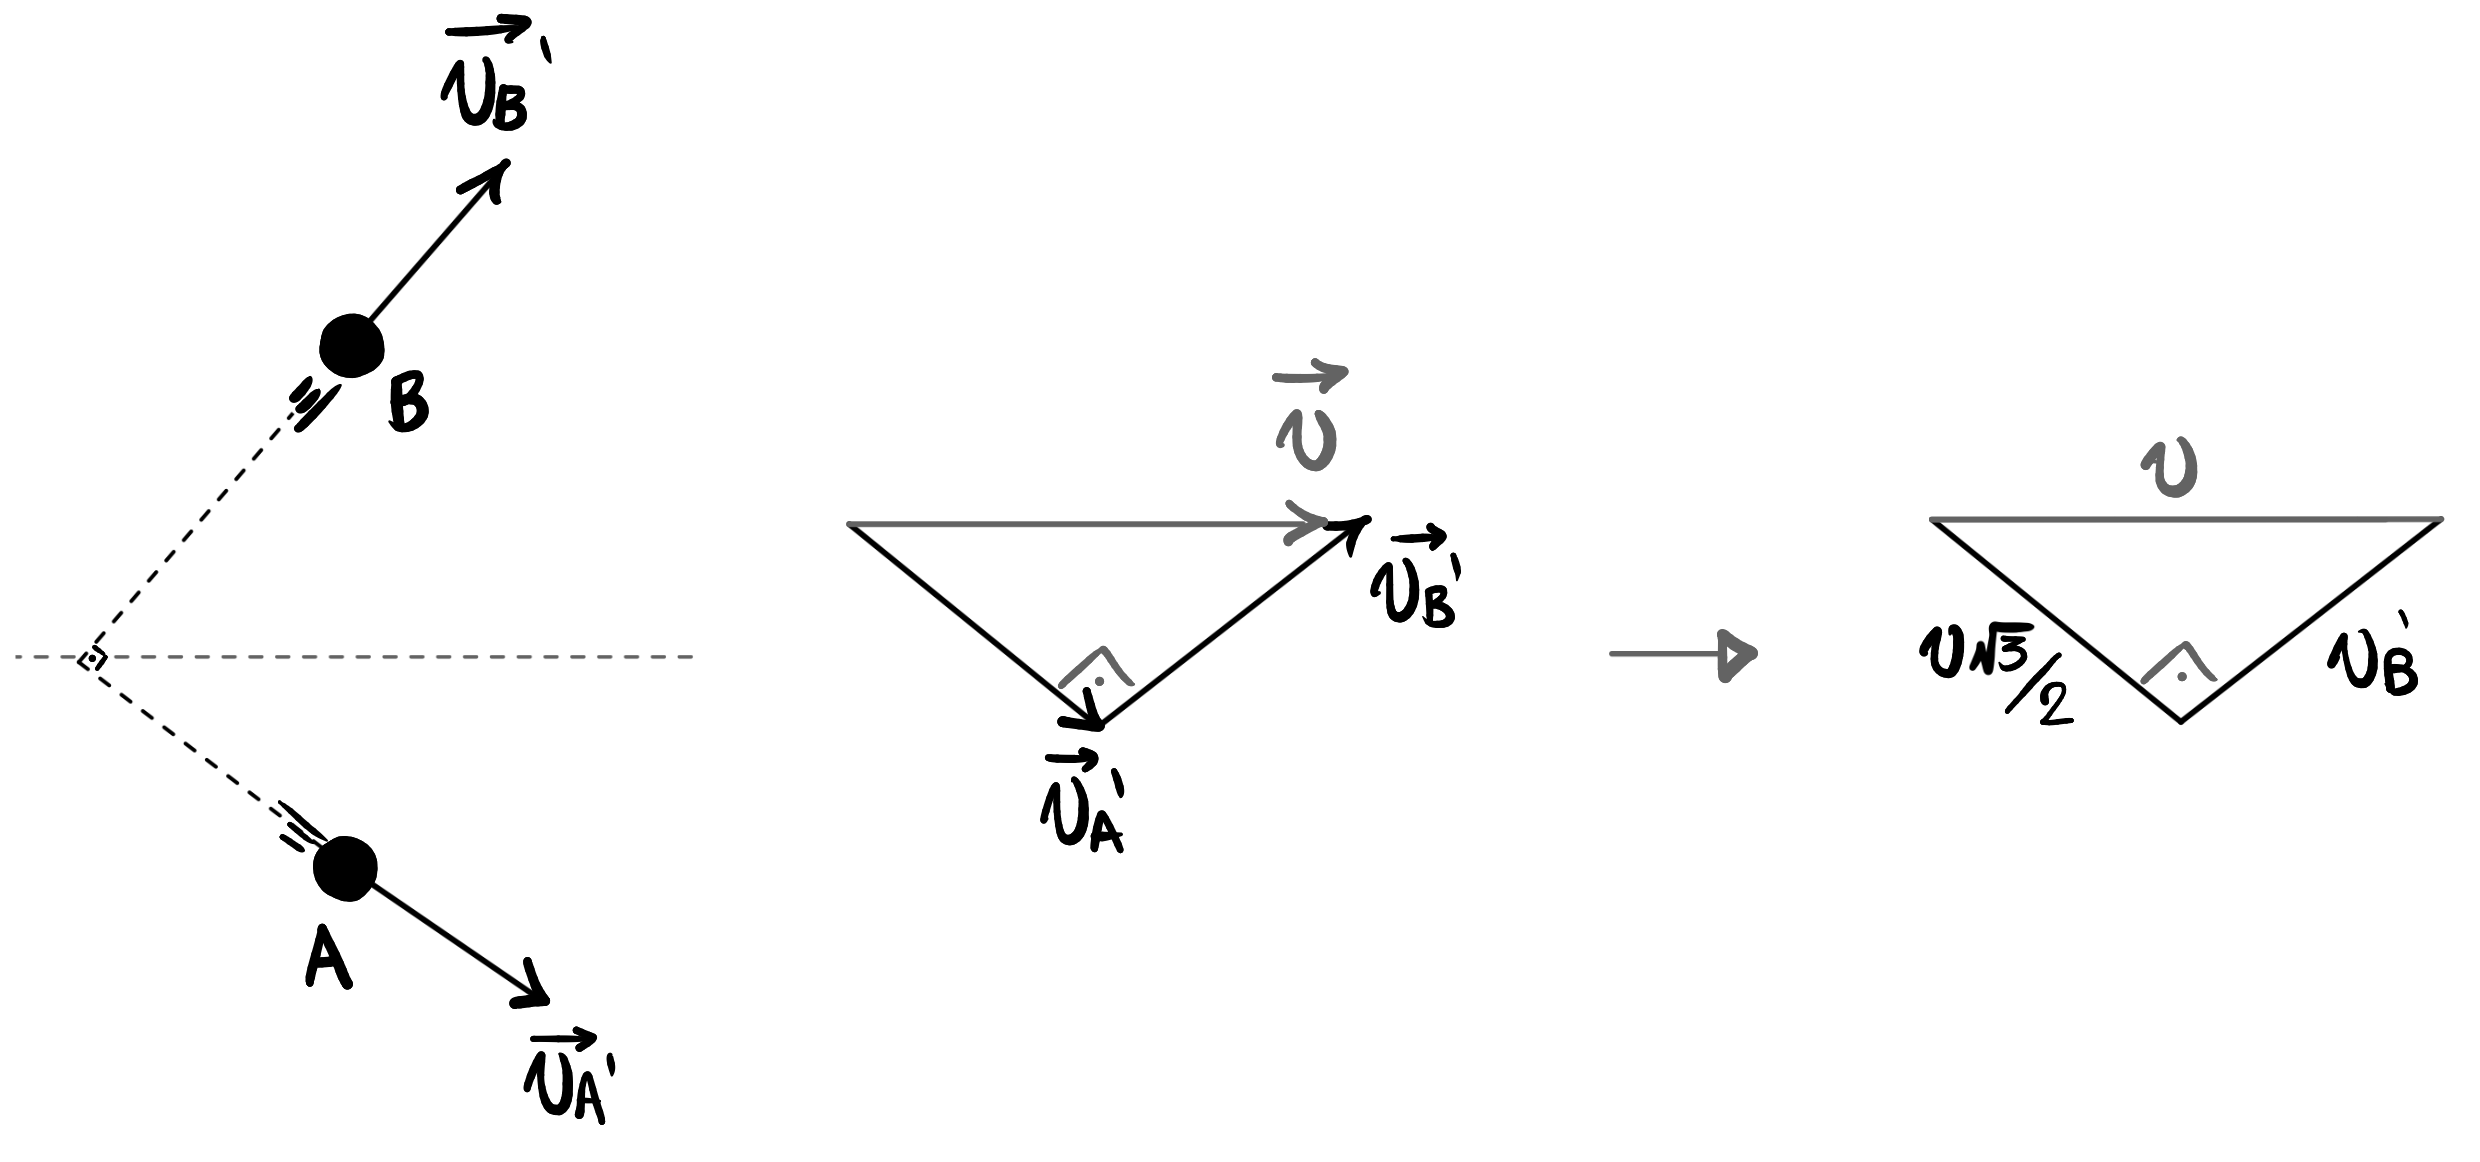
\includegraphics[width=0.8\linewidth]{imagensdinamicanewton/colisao2dqdm2.png}};
  \end{scope}
\end{tikzpicture}
\captionof{figure}{Análise vetorial das velocidades na colisão bidimensional entre duas partículas $A$ e $B$.}
\label{fig_newton_qdmcolisao2d02}
} 
\vspace{0.3cm}

Na última imagem da Figura \ref{fig_newton_qdmcolisao2d02} convertemos o problema para o campo puramente geométrico: temos um triângulo retângulo de lados $v$ e $\sfrac{v\sqrt 3}{2}$, e procuramos encontrar seu terceiro lado, $v_B',$ o que pode ser feito pelo Teorema de Pitágoras:

$$ v^2 = \left( \dfrac{v\sqrt 3}{2} \right)^2+ (v_B')^2 \implies \boxed{v_B'= \dfrac{v}{2} .}$$


\end{exemplo}

\vspace{0.3cm}

\begin{exemplo}[Nível III (ITA - 1998)]\label{exemplo_newton_conservacaomomentolinearex03}

As massas $m_1 = 3{,}0\,\text{kg}$ e $m_2 = 1{,}0\,\text{kg}$ foram fixadas nas extremidades de uma haste homogênea, de massa desprezível e 40 cm de comprimento. Este sistema foi colocado verticalmente sobre uma superfície plana, perfeitamente lisa, conforme mostra a figura, e abandonado. A massa $m_1$ colidirá com a superfície a uma distância $x$ do ponto $P$ dada por:

\begin{center}
\begin{tikzpicture}[scale=1.0]

    % parâmetros
    \def\rdois{0.18}
    \def\rum{0.30}

    % chão
    \draw[thick] (-1.4,0) -- (1.4,0);
    \foreach \x in {-1.3,-1.1,...,1.3}
        \draw[thick] (\x,0) -- (\x+0.15,-0.15);

    % ponto P
    \node at (0,-0.35) {$P$};

    % massa inferior m2 tangenciando o chão
    \draw[fill={}, thick] (0,\rdois) circle (\rdois);
    \node[right] at (0.22,\rdois) {$m_2$};

    % haste
    \draw[thick] (0,2*\rdois) -- (0,2.55);

    % massa superior m1
    \draw[fill={}, thick] (0,2.85) circle (\rum);
    \node[right] at (0.35,2.85) {$m_1$};

    % indicação do comprimento
    \node[right] at (0.22,1.55) {$40\ \text{cm}$};

\end{tikzpicture}
\end{center}


\begin{enumerate}
    \item [a)] $x = 0$ (no ponto $P$)
    \item [b)] $x = 10\,\text{cm}$
    \item [c)] $x = 20\,\text{cm}$
    \item [d)] $x = 30\,\text{cm}$
    \item [e)] $x = 40\,\text{cm}$
\end{enumerate}


\resolucao

Note que, na horizontal, não há nenhuma força externa ao sistema das massas $m_1$ e $m_2$ -- a única força externa é o peso, que é vertical. Sendo assim, quando as massas começarem a se movimentar, elas poderão ganhar momento linear na vertical, mas não na horizontal. Logo, temos um sistema isolado na horizontal, direção na qual haverá conservação do momento linear.

Assim, ao começar a girar, se a massa $m_1$ começar a se mover para a esquerda, a massa $m_2$ deverá começar a se mover para a direita, com o mesmo momento, haja vista que o momento inicial (na horizontal) era nulo. A primeira imagem da Figura \ref{fig_newton_qdmita} mostra isso. Matematicamente, teríamos, para a horizontal:

$$ p_{0x} = p_{fx} \implies 0 = m_1v_1 + m_2 v_2 \implies v_2 = - \dfrac{m_1}{m_2}v_1,$$

\noindent em que o sinal negativo indica apenas que as massas se movem em sentido contrários, como esperado. Escrevendo a relação acima apenas em valor absoluto, e usando a definição de velocidade, temos

$$ \dfrac{\Delta x_2}{ \cancel{\Delta t}} = \dfrac{m_1}{m_2} \dfrac{\Delta x_1}{ \cancel{\Delta t}} \implies \Delta x_2 = \dfrac{m_1}{m_2} \Delta x_1 \implies \boxed{\Delta x_2 = 3 \Delta x_1.} $$



{
\centering
\begin{tikzpicture}
  \begin{scope}[blend mode=multiply]
    \node {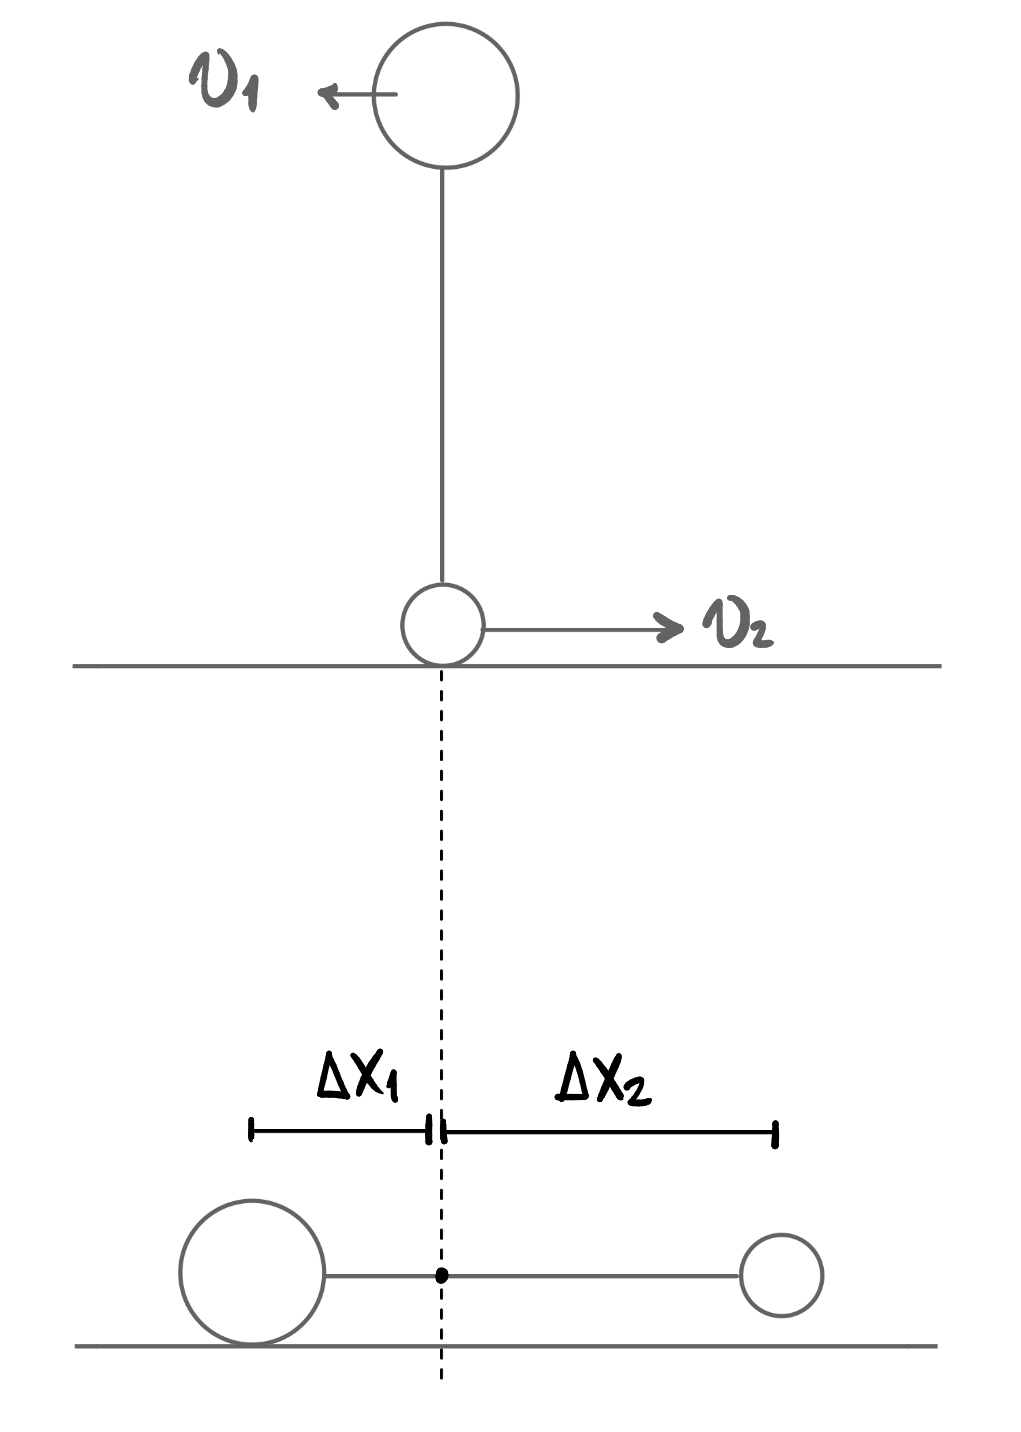
\includegraphics[width=0.35\linewidth]{imagensdinamicanewton/qdmita.png}};
  \end{scope}
\end{tikzpicture}
\captionof{figure}{}

\label{fig_newton_qdmita}
} 
\vspace{0.3cm}


Isso quer dizer que o deslocamento horizontal da massa $m_2$ deve ser o triplo daquele sofrido pela massa $m_1$ -- há de ser assim por conta da conservação do momento linear na horizontal. Logo, como mostra a imagem debaixo da Figura \ref{fig_newton_qdmita}, é preciso que $\Delta x_1 + \Delta x_2 = L = 40$ cm, logo:

$$ \Delta x_1 + 3 \Delta x_1 = 40 \implies \boxed{\Delta x_1 = 10 \text{ cm} \implies \text{ letra B.}}$$


\end{exemplo}


\vspace{0.3cm}














\newpage

\section{Equilíbrio de Corpo Extenso}







\begin{secnivel}[Torque de uma força]{I}{Torque de uma força}

  \eqLdois{def}{eq_newton_torque}{%
    \tau = F_{\perp} \cdot d \quad\text{ou}\quad
    \tau = F \cdot d \cdot \sin\theta
  }
\end{secnivel}


% \eqLdois{def}{eq_newton_torque}{$\tau$ = F_{\perp} \cdot d \quad \text{ ou } \quad  $\tau$ = F \cdot d \cdot \sin $\theta$}

 % Dizemos que uma força produz torque em relação a um ponto $O$
 %  quando ela tende a provocar uma rotação em torno desse ponto.





\secgfe{De onde vem}

A Equação \eqref{eq_newton_torque} calcula o torque gerado por uma força $F$ em relação a um certo ponto que dista $d$ do ponto de aplicação de tal força. 

O torque de uma força é definido como uma grandeza que mede a capacidade que uma força tem de produzir rotação. Considere a situação de uma barra, pivotada na parede no ponto $O$ e tendo, portanto, liberdade para girar em torno deste ponto. 

{
\centering
\begin{tikzpicture}
  \begin{scope}[blend mode=multiply]
    \node {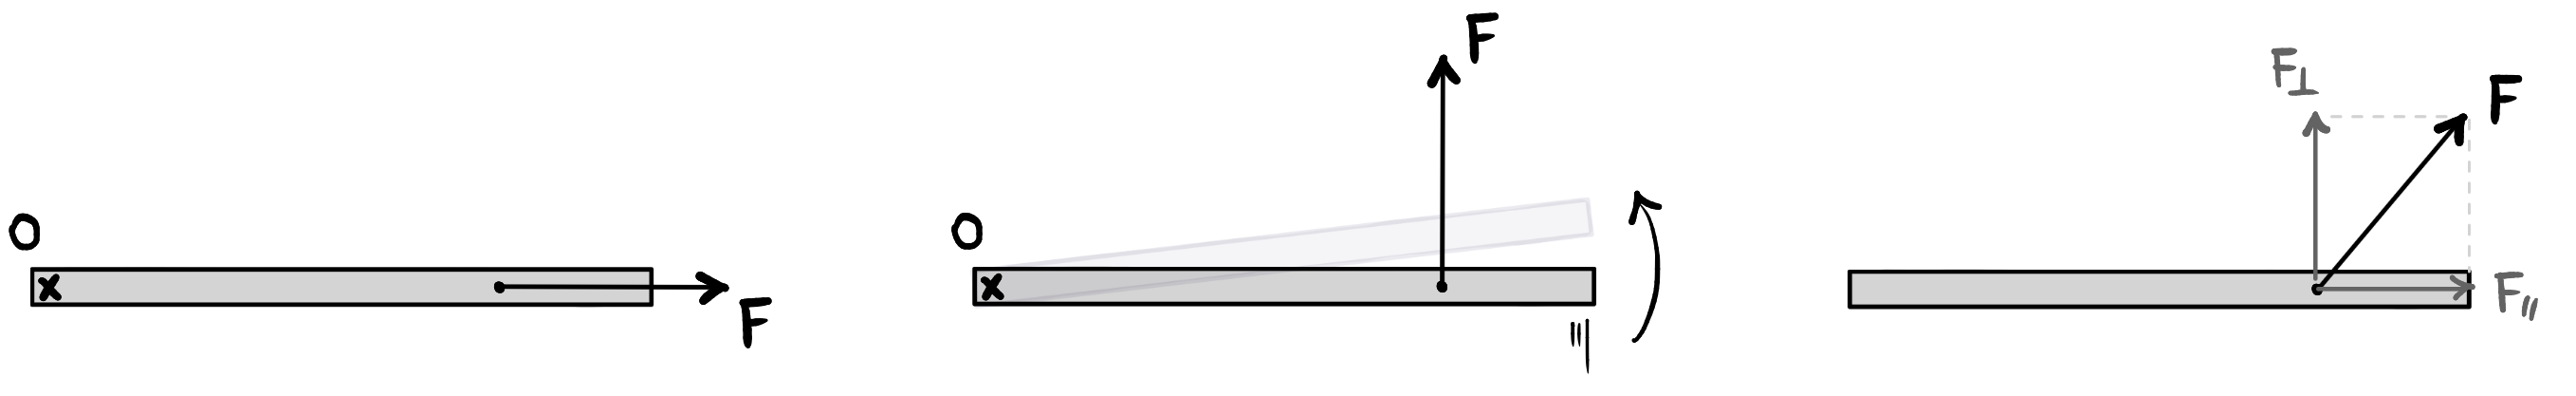
\includegraphics[width=1.0\linewidth]{imagensdinamicarotacao/torquedefinicao.png}};
  \end{scope}
\end{tikzpicture}
\captionof{figure}{Forças perpendiculares à barra produzem rotação, forças paralelas não.}

\label{fig_dinamicarotacao_torquedefinicao}
} 
\vspace{0.3cm}



É fácil ver que na situação da primeira imagem a força $F$ aplicada não irá gerar rotação em torno do ponto $O$ -- o leitor pode fazer o experimento por si só e atestar isso: segure, em cima de uma mesa, a extremidade uma caneta; ao tentar puxar a outra extremidade o sistema continua parado. Conclui-se, portanto, que forças paralelas à barra não geram torque (rotação)\footnote{Forças paralelas a barra são responsáveis por deformar a barra -- comprimi-la ou esticá-la --, mas não geram rotação.}.

Já no segundo caso o leitor pode verificar que a barra começaria a girar em torno do ponto $O,$ ou seja, forças perpendiculares à barra geram torque.

A terceira imagem ilustra um caso intermediário: a força $F$ aplicada não está totalmente alinhada com a direção da barra, mas também não está integralmente na direção perpendicular à barra. Neste caso, o protocolo seria decompor a força, que teria uma componente paralela à barra, $F_{//}$, que não produz torque. A outra componente, perpendicular à barra, $F_\perp,$ é a responsável por gerar o torque. 


{
\centering
\begin{tikzpicture}
  \begin{scope}[blend mode=multiply]
    \node {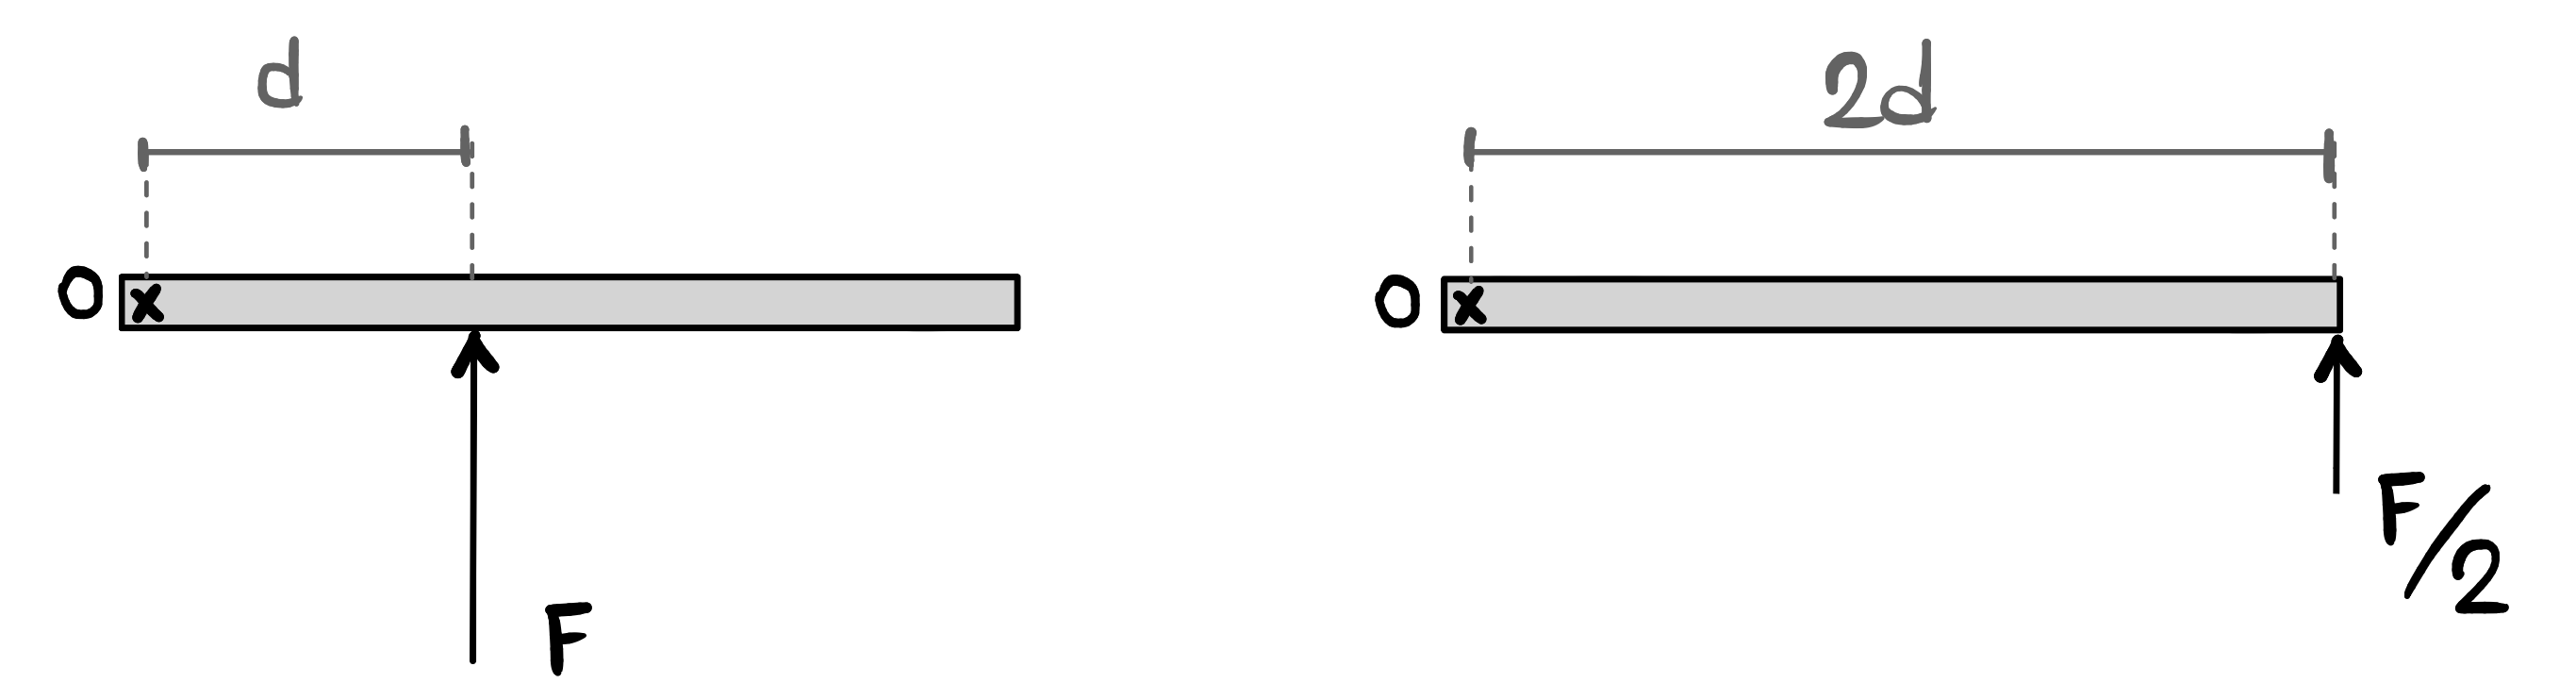
\includegraphics[width=0.75\linewidth]{imagensdinamicarotacao/torquedefinicao02.png}};
  \end{scope}
\end{tikzpicture}
\captionof{figure}{Quanto maior a distância em relação ao ponto $O,$ mais fácil é de gerar rotação.}
\label{fig_dinamicarotacao_torquedefinicao02}
} 
\vspace{0.3cm}

A Figura \ref{fig_dinamicarotacao_torquedefinicao02} mostra um outro experimento, que pode ser facilmente realizado pelo leitor. É fácil perceber que, quanto mais afastado for o ponto de aplicação da força em relação ao ponto fixo (também chamado de pivô), isto é, quanto maior for a distância $d$ (também chamada de braço de alavanca), mais fácil é para que a força produza rotação. É possível, por exemplo, gerar a mesma rotação usando metade da força, caso se use o dobro do braço de alavanca.

Sendo assim, vemos que a rotação que uma força produz é proporcional à componente da força perpendicular à barra, isto é, $F_\perp$, e também ao braço de alavanca $d$ -- a distância do ponto de aplicação da força até o ponto em relação ao qual estamos tomando os torques. Desse modo, é natural definir o torque de uma força pela Equação \eqref{eq_newton_torque}: o torque e definido como sendo o produto dessas duas grandezas, $F_\perp$ e $d.$

A segunda forma de se escrever a Equação \eqref{eq_newton_torque} já considera o vetor $F$ decomposto. O ângulo $\theta,$ neste caso, é o ângulo entre a força $F$ e a direção da barra, como mostra a Figura \ref{fig_dinamicarotacao_torqueangulo}, em que uma trigonometria simples nos mostra que 

$$ \sin \theta = \dfrac{F_\perp}{F} \implies \boxed{F_\perp = F \sin \theta,} $$

\noindent de modo que o torque fica sendo $\tau = F_\perp \cdot d = F \sin \theta \cdot  d, $ como mostra a Equação \eqref{eq_newton_torque}.


{
\centering
\begin{tikzpicture}
  \begin{scope}[blend mode=multiply]
    \node {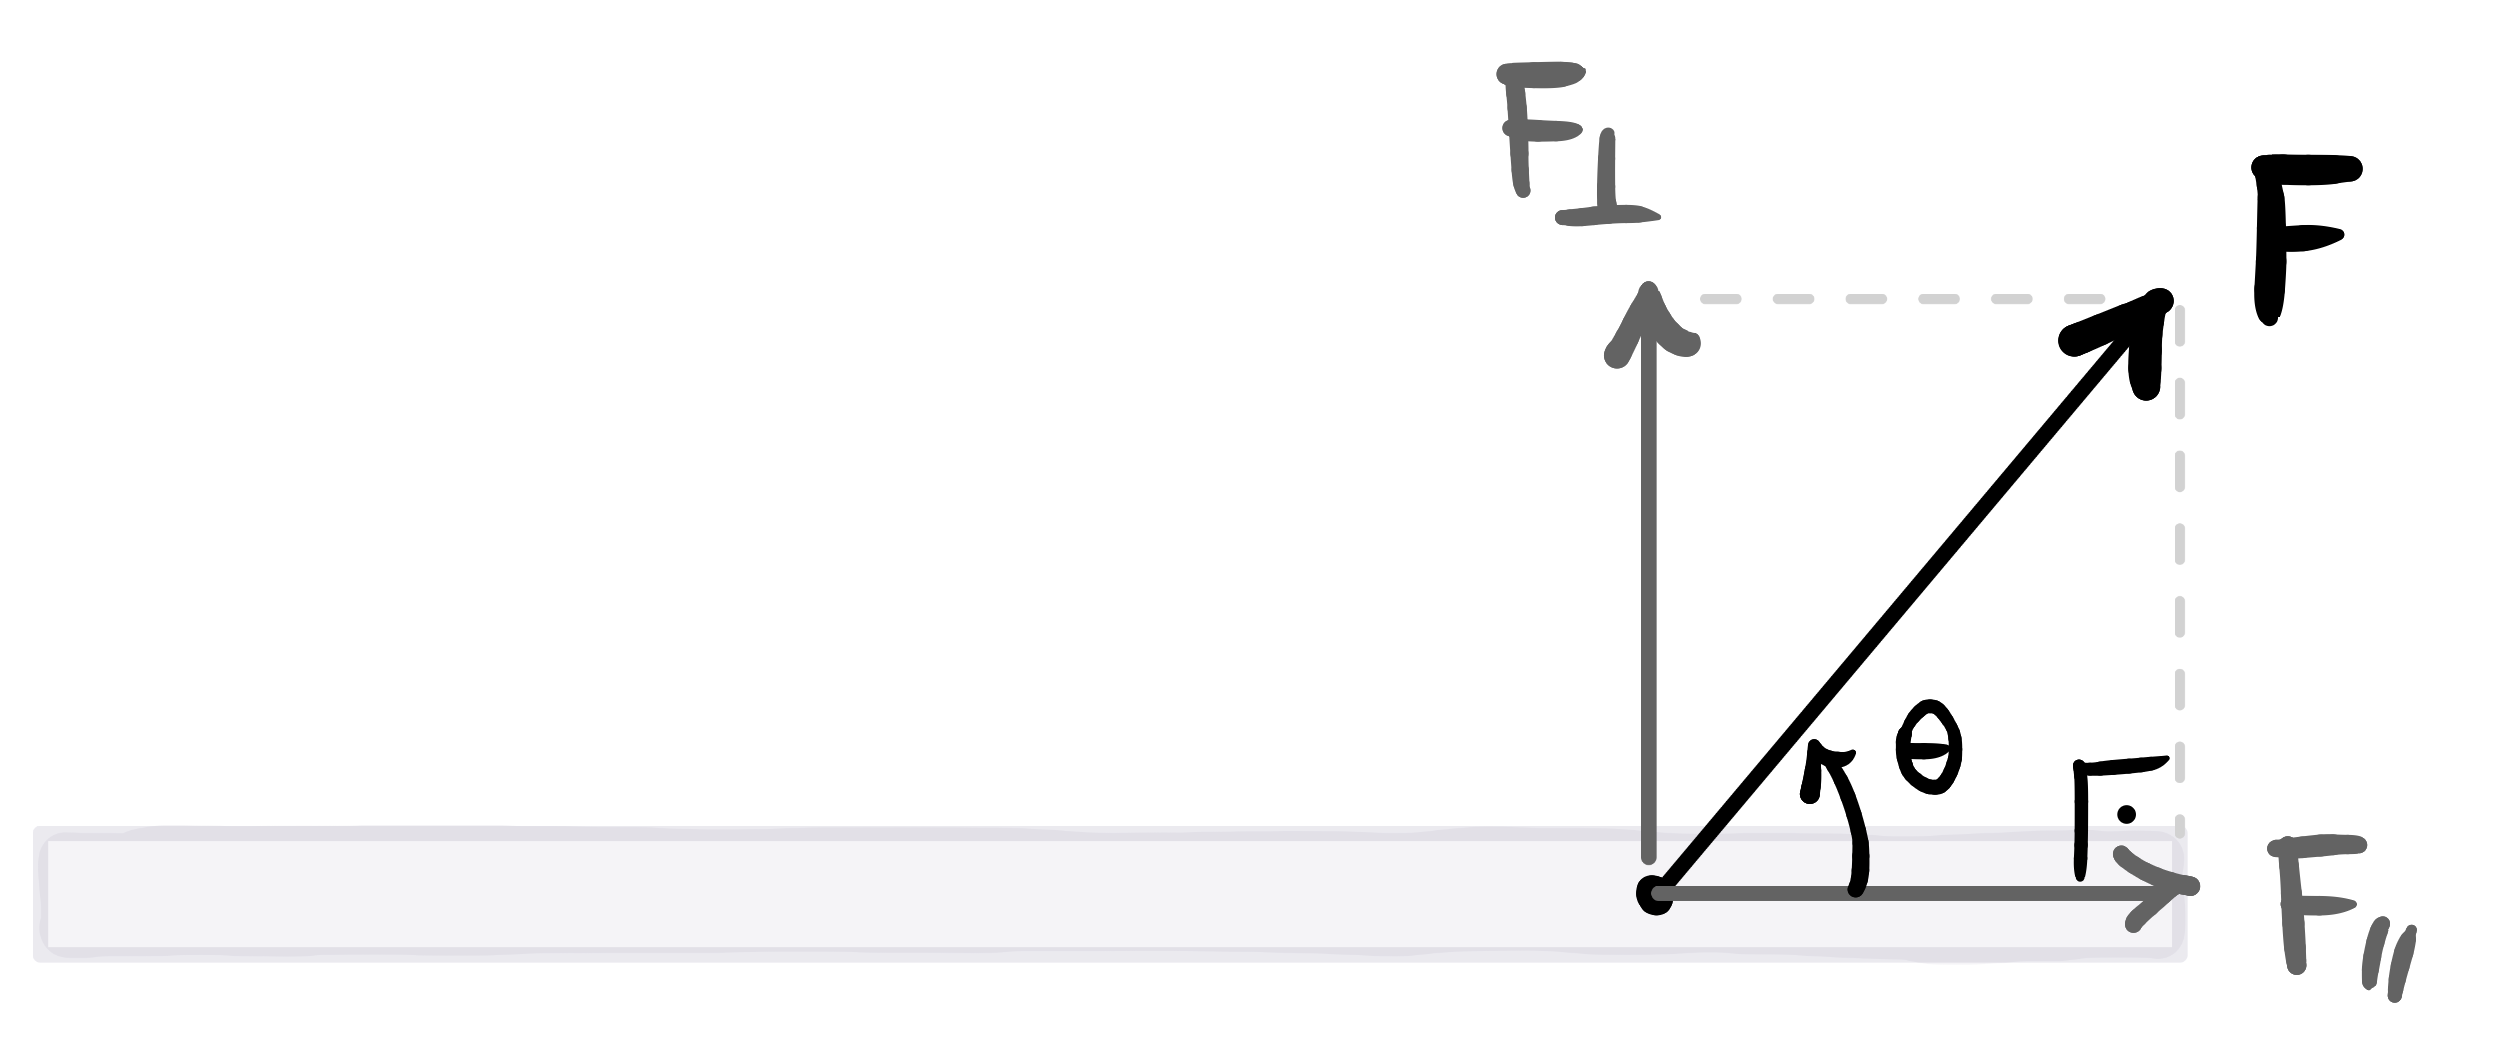
\includegraphics[width=0.4\linewidth]{imagensdinamicarotacao/torqueangulo.png}};
  \end{scope}
\end{tikzpicture}
\captionof{figure}{Decomposição da força $F$ para avaliar a componente responsável pela rotação, $F_\perp.$.}
\label{fig_dinamicarotacao_torqueangulo}
} 
\vspace{0.3cm}




\secgfe{Onde é usada}

O conceito de torque será usado em quaisquer problemas que envolvam a dinâmica de corpos rígidos e extensos, mais especificamente, o seu equilíbrio, no contexto do Ensino Médio. Note que, para uma partícula, a condição descrita pela Equação \eqref{eq_newton_equilibriof=0} é suficiente para garantir que tal partícula está em equilíbrio, isto é, em repouso ou em MRU.

\vspace{0.3cm}
{
\centering
\begin{tikzpicture}
  \begin{scope}[blend mode=multiply]
    \node {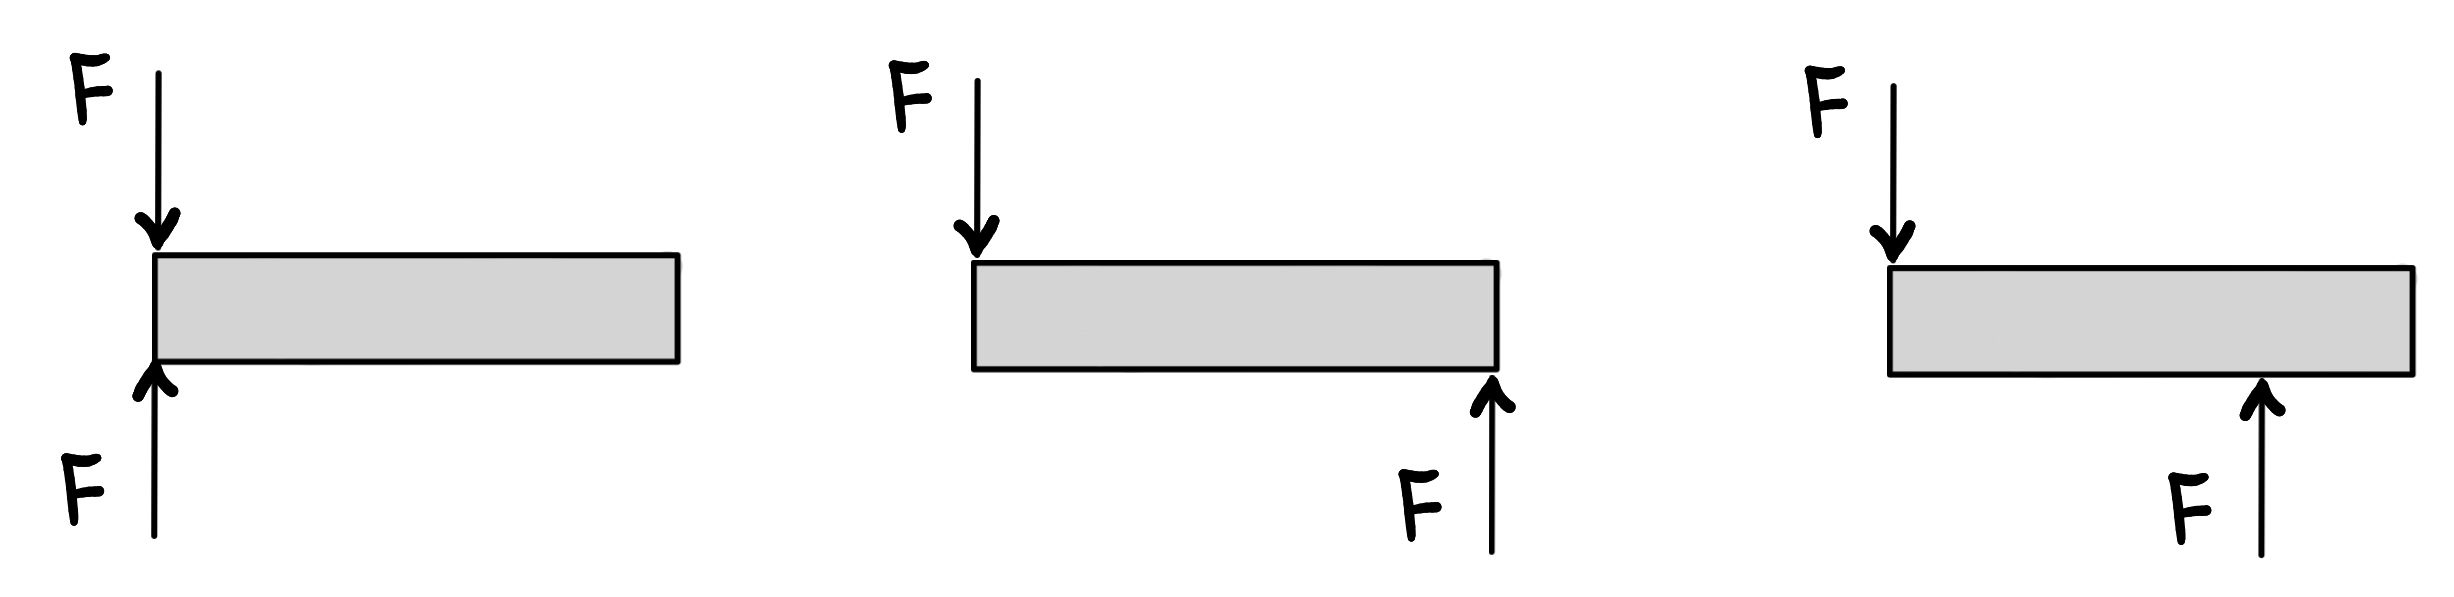
\includegraphics[width=0.6\linewidth]{imagensdinamicarotacao/torque01.png}};
  \end{scope}
\end{tikzpicture}
\captionof{figure}{A condição $F_{\text{R}}=0$ não garante o equilíbrio para corpos extensos.}

\label{fig_dinamicarotacao_torque01}
} 
\vspace{0.3cm}

Considere, contudo, as situações da Figura \ref{fig_dinamicarotacao_torque01}. Nas três situações a condição da Equação \eqref{eq_newton_equilibriof=0} é satisfeita, isto é, temos que $F_{\text{R}}=0.$ Contudo, apenas na primeira delas há, de fato, uma situação de equilíbrio. Nas duas outras situações a barra estará girando, ainda que, nos dois casos, tenha-se $F_{\text{R}}=0.$ Ou seja, a força resultante é zero mas o corpo não está parado, nem em MRU: ele estará girando -- cada vez mais rápido, inclusive.

Tudo isso ocorre porque a condição de equilíbrio proposta na Equação \eqref{eq_newton_equilibriof=0} é válida para uma partícula, ou seja, um corpo pontual, de dimensões desprezíveis. Note que um ponto só possui três tipos de movimentos possíveis: transladar para cima (ou para baixo), para a direita (ou esquerda) e para frente (ou para trás). Como um ponto não pode rotacionar -- apenas transladar -- quando garantimos que $F_{\text{R}}=0$ estamos garantindo, automaticamente, o seu equilíbrio.

Já para um corpo extenso, ele pode girar em torno de vários pontos. Logo, a condição $F_{\text{R}}=0$ garante que ele não estará transladando de forma acelerada, mas não garante que ele não estará girando. Dessa forma, precisamos ampliar a condição de equilíbrio expressa na Equação \eqref{eq_newton_equilibriof=0} para abranger os corpos extensos. Para tal, é preciso garantir, além do equilíbrio de translação, o equilíbrio de rotação; ou seja:

\begin{equation}
     \boxed{\tau_\text{R} = 0.}
    \label{eq_newton_torque=zero}
\end{equation}

Dessa maneira, para que um corpo extenso (de dimensões não desprezíveis) esteja parado, é preciso satisfazer as duas condições:


$$ \text{Equilíbrio de Translação: } \boxed{F_{\text{R}}=0}  \quad  \text{ e } \quad \text{Equilíbrio de Rotação: } \boxed{\tau_\text{R} = 0}$$

Considere o problema da Figura \ref{fig_dinamicarotacao_torque02}, que mostra uma barra de comprimento $L$ e massa desprezível, apoiada sob o seu centro. Em uma extremidade coloca-se uma caixa $A$, de massa $m$. Entre o ponto médio da barra e a outra extremidade, coloca-se outra caixa $B.$ Qual deve ser sua massa para que a barra fique em equilíbrio?

\vspace{0.3cm}
{
\centering
\begin{tikzpicture}
  \begin{scope}[blend mode=multiply]
    \node {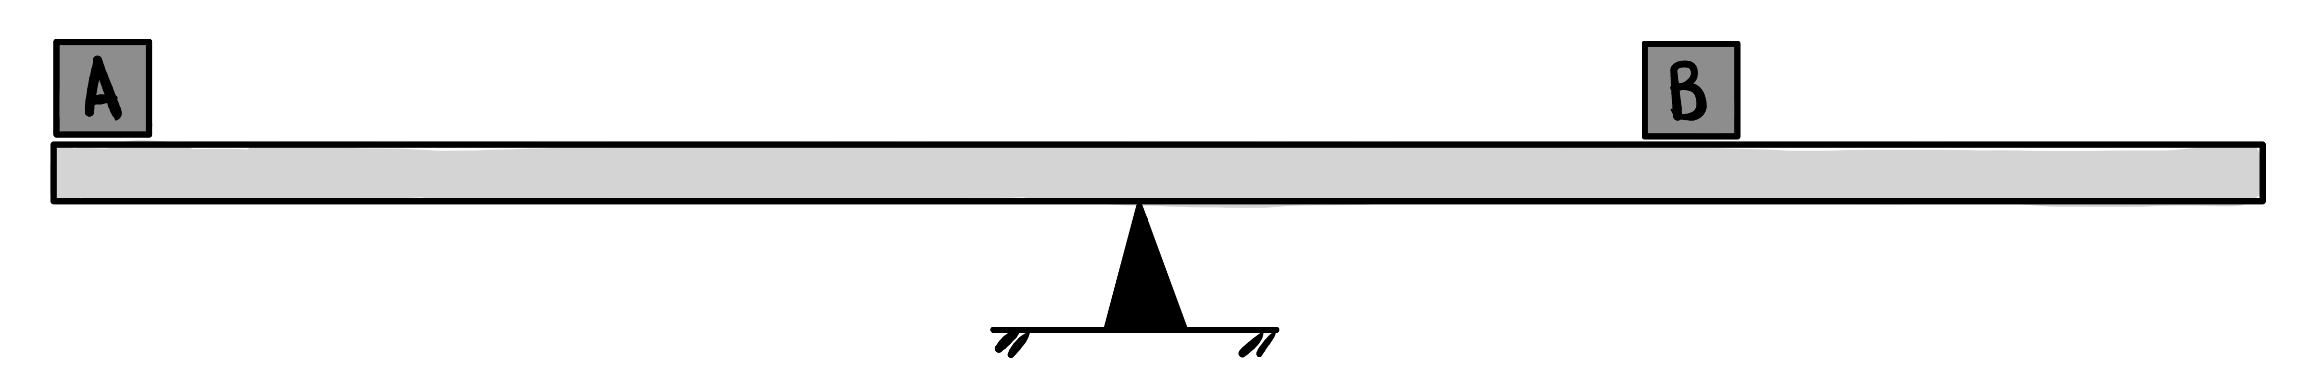
\includegraphics[width=0.6\linewidth]{imagensdinamicarotacao/torque021.png}};
  \end{scope}
\end{tikzpicture}
\captionof{figure}{Barra de massa desprezível apoiada sob o seu centro.}
\label{fig_dinamicarotacao_torque02}
} 
\vspace{0.3cm}

A Figura \ref{fig_dinamicarotacao_torque03} mostra o diagrama de forças sob a barra: nas posições das caixas a barra sofrerá forças normais, verticais para baixo, iguais ao peso de cada caixa\footnote{De forma rigorosa, a força que a barra sente não é o peso da caixa: este atua na caixa. Contudo, por estar apoiada na barra, a caixa sente uma força normal, feita pela barra. Como o sistema todo está em equilíbrio, a normal na caixa é igual ao seu peso. Pela Terceira Lei de Newton, a caixa devolve uma força normal $N$, vertical e para baixo, na barra. Tal força, em módulo, é igual ao peso da caixa.}, enquanto que, no centro, por estar sendo comprimida contra o apoio, a barra empurrará o apoio para baixo, que reagirá, fazendo uma força normal $N,$ igual e contrária na barra.


\vspace{0.3cm}
{
\centering
\begin{tikzpicture}
  \begin{scope}[blend mode=multiply]
    \node {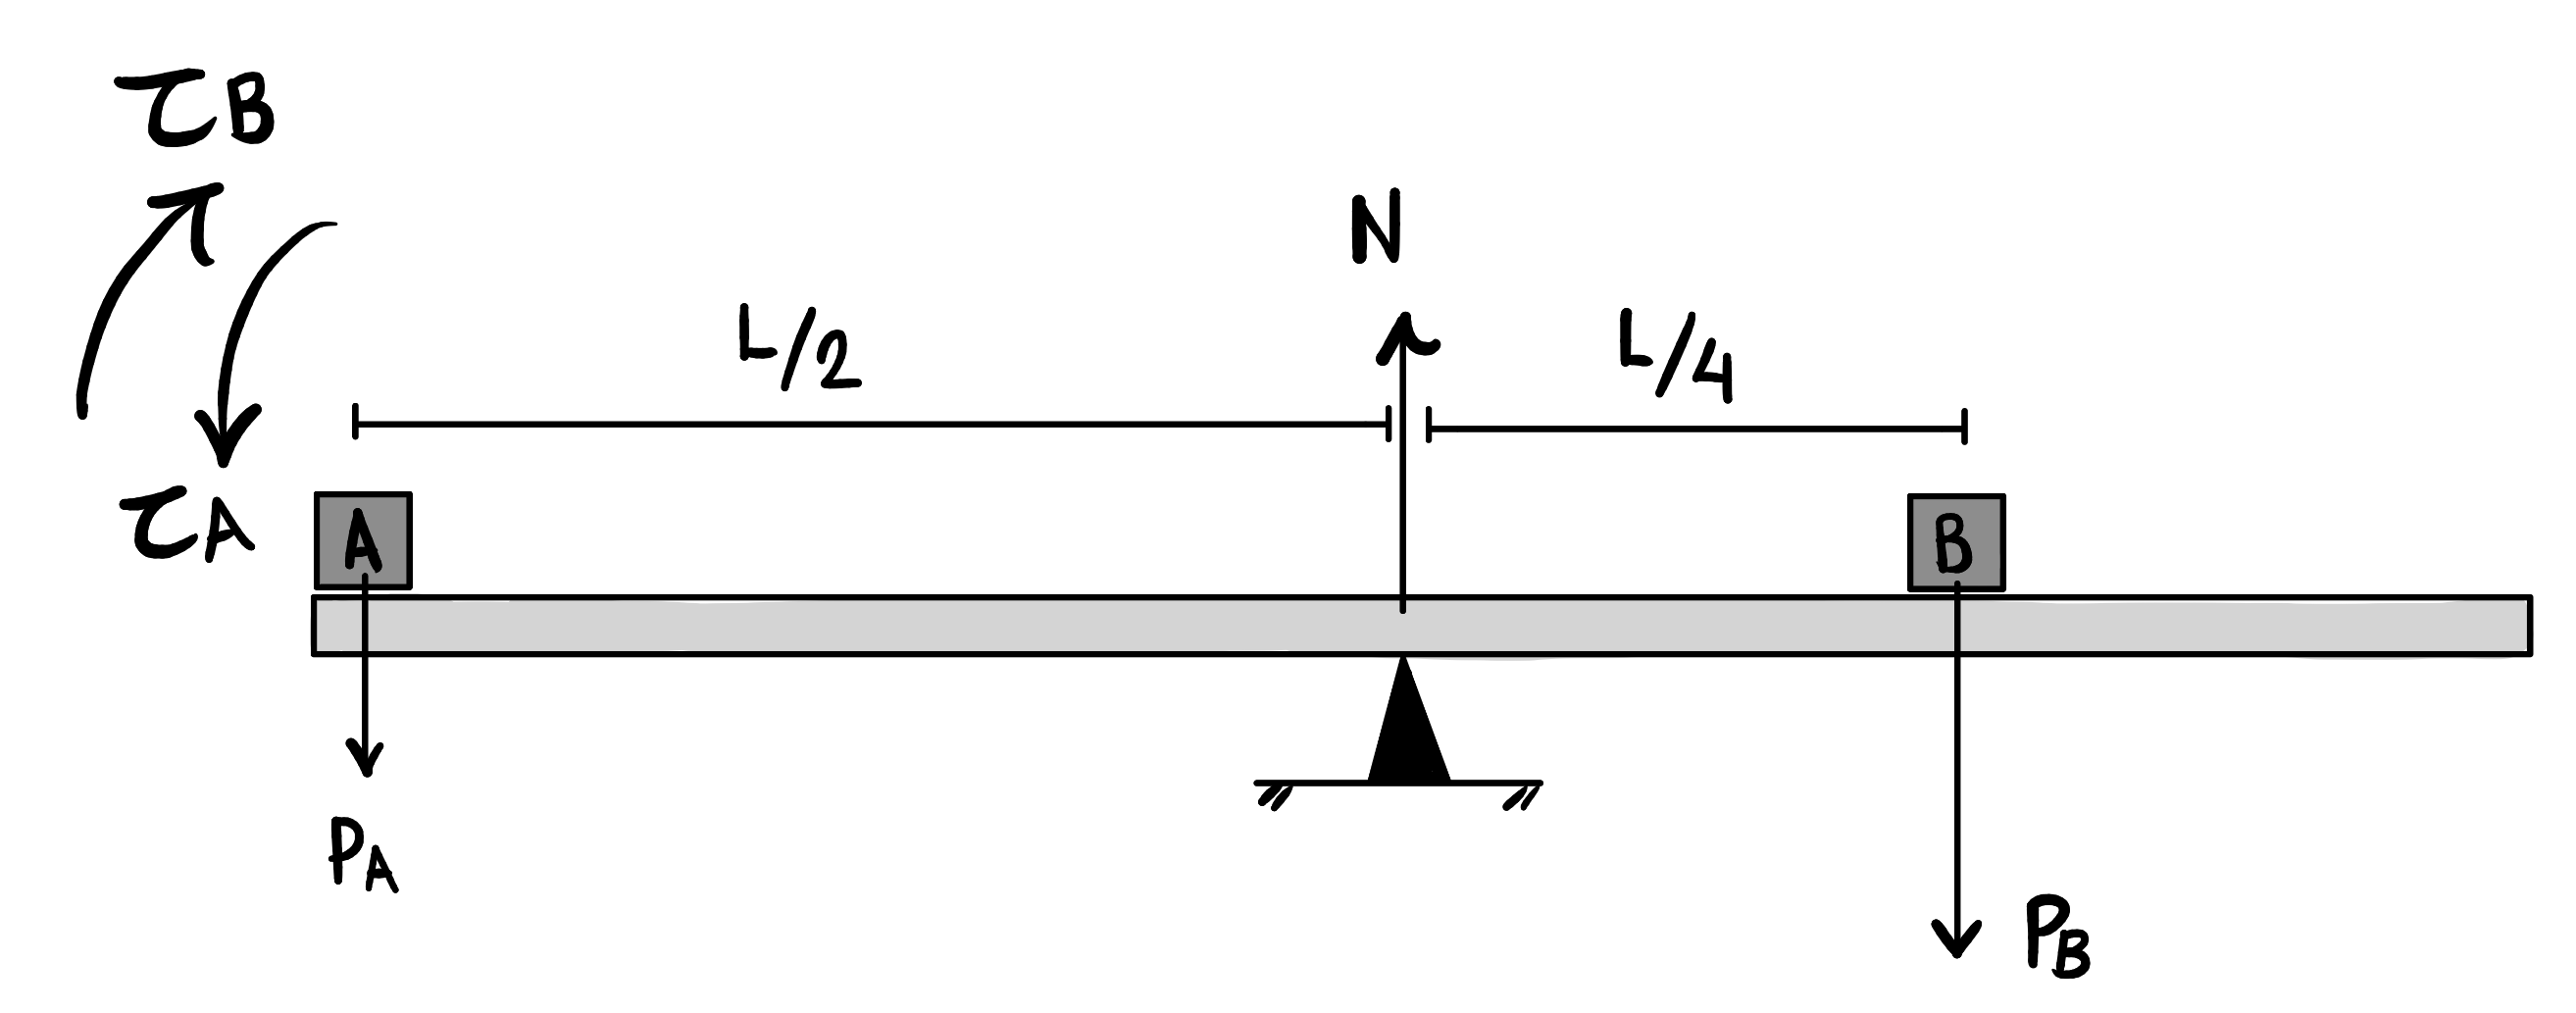
\includegraphics[width=0.6\linewidth]{imagensdinamicarotacao/torque022.png}};
  \end{scope}
\end{tikzpicture}
\captionof{figure}{Diagrama de forças e torques sob a barra.}
\label{fig_dinamicarotacao_torque03}
} 
\vspace{0.3cm}


É fácil ver que, em relação ao ponto de apoio, a caixa $A$, devido ao seu peso, tende a girar a barra no sentido anti-horário, enquanto que a caixa $B$, por conta de seu peso, tende a girar a barra no sentido horário. Perfeito: só precisamos que tais torques se equilibrem.\footnote{A normal feita pelo apoio na barra não gera torque porque sua distância $d$ até o ponto em relação ao qual estamos tomando os torques é zero, isto é, a força atua no próprio ponto tomado como referência para se calcular os torques. Logo, usando a Equação \eqref{eq_newton_torque}, vemos que o torque de tal força é nulo. Este é um princípio importante: todas as forças que atuarem no próprio pivô (ponto em relação ao qual estamos calculando os torques) não produzirão torque.} Logo, exigimos que:

$$ \tau_\text{R} = 0 \implies \tau_\text{A} = \tau_\text{B} \implies P_\text{A} \cdot \dfrac{L}{2} = P_\text{B} \cdot \dfrac{L}{4} \implies P_\text{B} = 2 P_\text{A},$$

\noindent ou seja, para que haja equilíbrio de rotação é preciso que a massa da caixa $B$ seja o dobro da massa da caixa $A.$ Logo, sendo $m_\text{A}=m$, teremos que $\boxed{m_\text{B} = 2m.}$

Note que este é um resultado razoável, que poderia ter sido obtido até sem desenvolver os cálculos. Sendo o torque proporcional à força e ao braço de alavanca $d$, para que duas forças diferentes (os pesos das caixas $A$ e $B,$ no caso) produzam o mesmo torque, é preciso que o produto de $F$ por $d$ das duas sejam iguais. Logo, a caixa que estiver na metade da distância $d$ (caixa $B)$ precisará exercer o dobro de força para compensar isto, a fim de gerar o mesmo torque. Logo, concluiríamos que a caixa $B$ precisaria ter o dobro de peso da caixa $A$ e, portanto, o dobro de massa. Razoável, não?

Perceba que seria possível, inclusive, computarmos o valor da normal que o apoio exerce na barra, exigindo que se satisfação a outra condição de equilíbrio, isto é, que 

$$ F_\text{R} = 0 \implies N = P_\text{A} + P_\text{B} \implies N = 3mg.$$

O leitor consegue compreender, intuitivamente, a razão de ser este o valor da força normal?


\secgfe{Erros comuns}

Um erro bastante comum é o estudante se confundir na decomposição e acabar não pegando a componente perpendicular de força, que é a que gera o torque. Como mostra a primeira notação da Equação \eqref{eq_newton_torque}, o importante é que estudante compreenda que é a componente de força $F_\perp$, perpendicular à barra, que irá produzir rotação.

Uma outra confusão comum é quando o estudante não percebe que o cálculo do torque pressupõe a escolha de um ponto de referência em relação ao qual computamos o torque. Considere, por exemplo, a situação da Figura \ref{fig_dinamicarotacao_torque02}. Parece natural que o ``correto'' é tomarmos os torques em relação ao ponto de apoio, porque a barra tende a girar em torno dele. Contudo, tal ponto é completamente arbitrário: é possível provar que, se os torques se anulam em relação a um ponto, eles se anulam em relação a qualquer outro ponto -- ainda que tal ponto sequer pertença ao corpo rígido em questão. Desse modo, para garantir o equilíbrio de rotação, basta que os torque se anulem em relação a um ponto qualquer.

Ainda na mesma situação, suponha que tenhamos escolhido o ponto da extremidade esquerda, aonde se encontra a massa $A$, para computar os torques. Neste caso, o torque devido ao peso da massa $A$ seria nulo; o torque devido à normal, no ponto de apoio, tenderia a girar a barra no sentido anti-horário; e o torque devido ao peso da massa $B$ tenderia a girá-la no sentido horário. Equilibrando esses dois últimos teríamos

$$ \tau_{\text{R}_{A}} = 0 \implies N \dfrac{L}{2} = P_\text{B} \left(\dfrac{L}{2} + \dfrac{L}{4}  \right)\implies N = \dfrac{3P_\text{B}}{2},$$

\noindent e, usando o resultado prévio de que $P_B=2mg$, chegamos que $N=3mg,$ que é exatamente o resultado que havíamos obtido no desenvolvimento deste caso, exigindo que $F_\text{R}=0.$

Note que as distâncias tomadas, na equação $F_\perp \cdot d,$ são as distâncias, neste caso, até o ponto $A$, que é o ponto de referência para o cálculo dos torques. A notação $\tau_{\text{R}_{A}} $ indica isso: estamos calculando o torque resultante em relação ao ponto $A.$

Desse modo, é importante deixar claro que, para garantir que um corpo esteja em equilíbrio de rotação, isto é, que o torque resultante seja zero, o ponto em relação ao qual tomamos os torques é arbitrário. É mais comum tomarmos como ponto de referência o ponto em torno do qual o corpo aparentemente tende a girar. Contudo, nem sempre isso é claro, como no caso da Figura \ref{fig_dinamicarotacao_torque2apoios}, em que podem haver dois ou mais apoios e não está exatamente claro em relação a qual ponto a barra poderá estar na iminência de girar.

\vspace{0.3cm}
{
\centering
\begin{tikzpicture}
  \begin{scope}[blend mode=multiply]
    \node {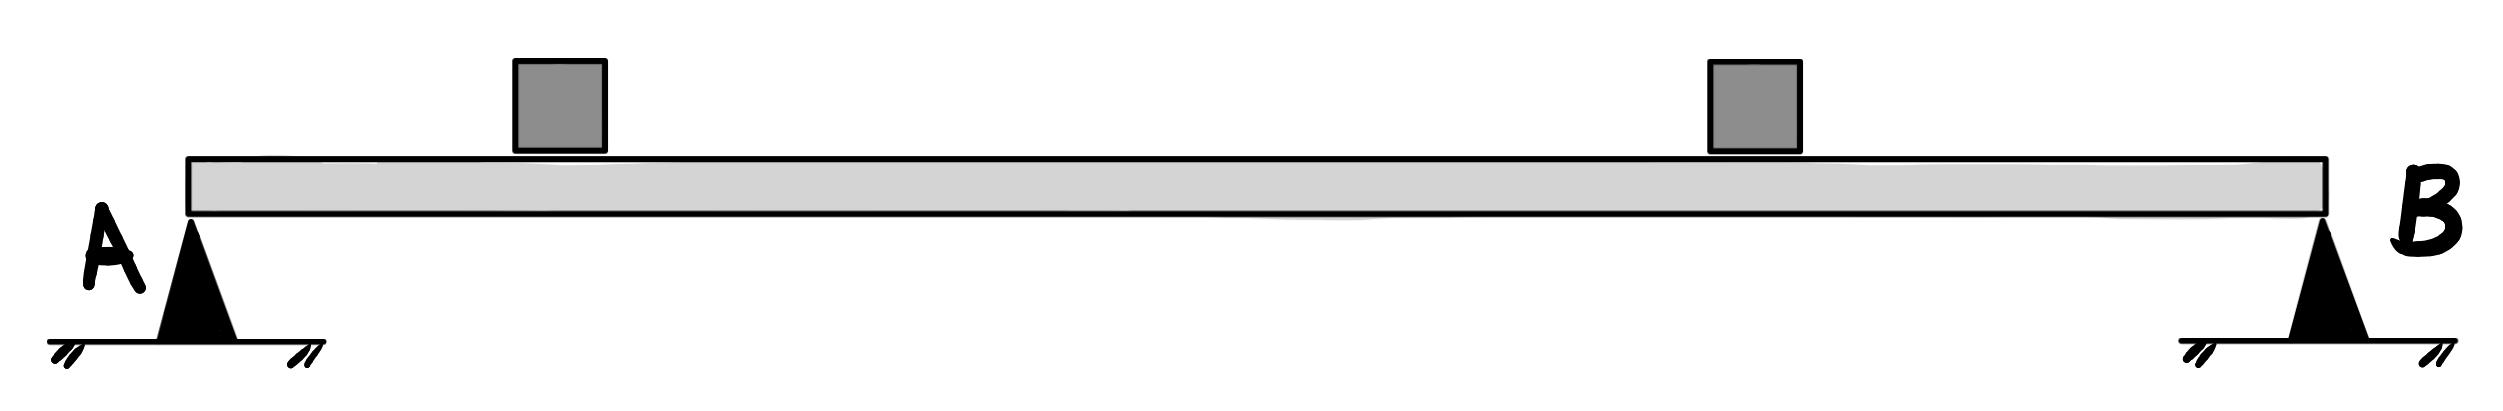
\includegraphics[width=0.7\linewidth]{imagensdinamicarotacao/torque2apoios.png}};
  \end{scope}
\end{tikzpicture}
\captionof{figure}{Barra com mais de um apoio.}
\label{fig_dinamicarotacao_torque2apoios}
} 
\vspace{0.3cm}

Assim, em situações como a da Figura \ref{fig_dinamicarotacao_torque2apoios}, para garantir o equilíbrio de rotação basta exigir que o torque se anule em relação a um certo ponto: pode ser o apoio $A$, o apoio $B$ ou outro ponto qualquer.

Uma outra situação que vale mencionar aqui é sobre barras que possuam peso. No contexto da Figura \ref{fig_dinamicarotacao_torque02} pontuamos que a barra tinha massa desprezível. Contudo, nem sempre isso acontece. 

Quando a barra tiver massa, consideraremos que a sua força peso atua em um único ponto, o seu \textit{centro de massa},\footnote{Um estudo mais detalhado e profundo sobre o centro de massa será feito no desenvolvimento da Equação \eqref{eq_newtonrotacao_posicaocentrodemassa}.} que é o ponto no qual podemos imaginar que toda a massa do corpo está concentrada. Tal ponto, para corpos homogêneos, isto é, corpos cuja distribuição de massa seja uniforme, coincide com o seu centro geométrico. Assim, para situações como as das Figuras \ref{fig_dinamicarotacao_torque02} ou \ref{fig_dinamicarotacao_torque2apoios}, caso as barras também possuam massa, consideraremos sua força peso atuando no seu centro geométrico: o meio da barra. 

Dito isso, é um erro bem comum entre os estudantes acabar esquecendo de colocar o peso da barra no diagrama de forças (nas situações em que a barra tem peso, claro), ou então colocar o seu peso em situações na qual a massa da barra é desprezível (a qual consideramos como sendo nula).


\secgfe{Observações}

Uma observação interessante é que, ao invés de decompor a força, tomando sua componente perpendicular à barra, é possível decompor a distância -- o braço de alavanca -- e obter o mesmo resultado do torque. Em alguns momentos será mais interessante proceder no cálculo por este caminho.

{
\centering
\begin{tikzpicture}
  \begin{scope}[blend mode=multiply]
    \node {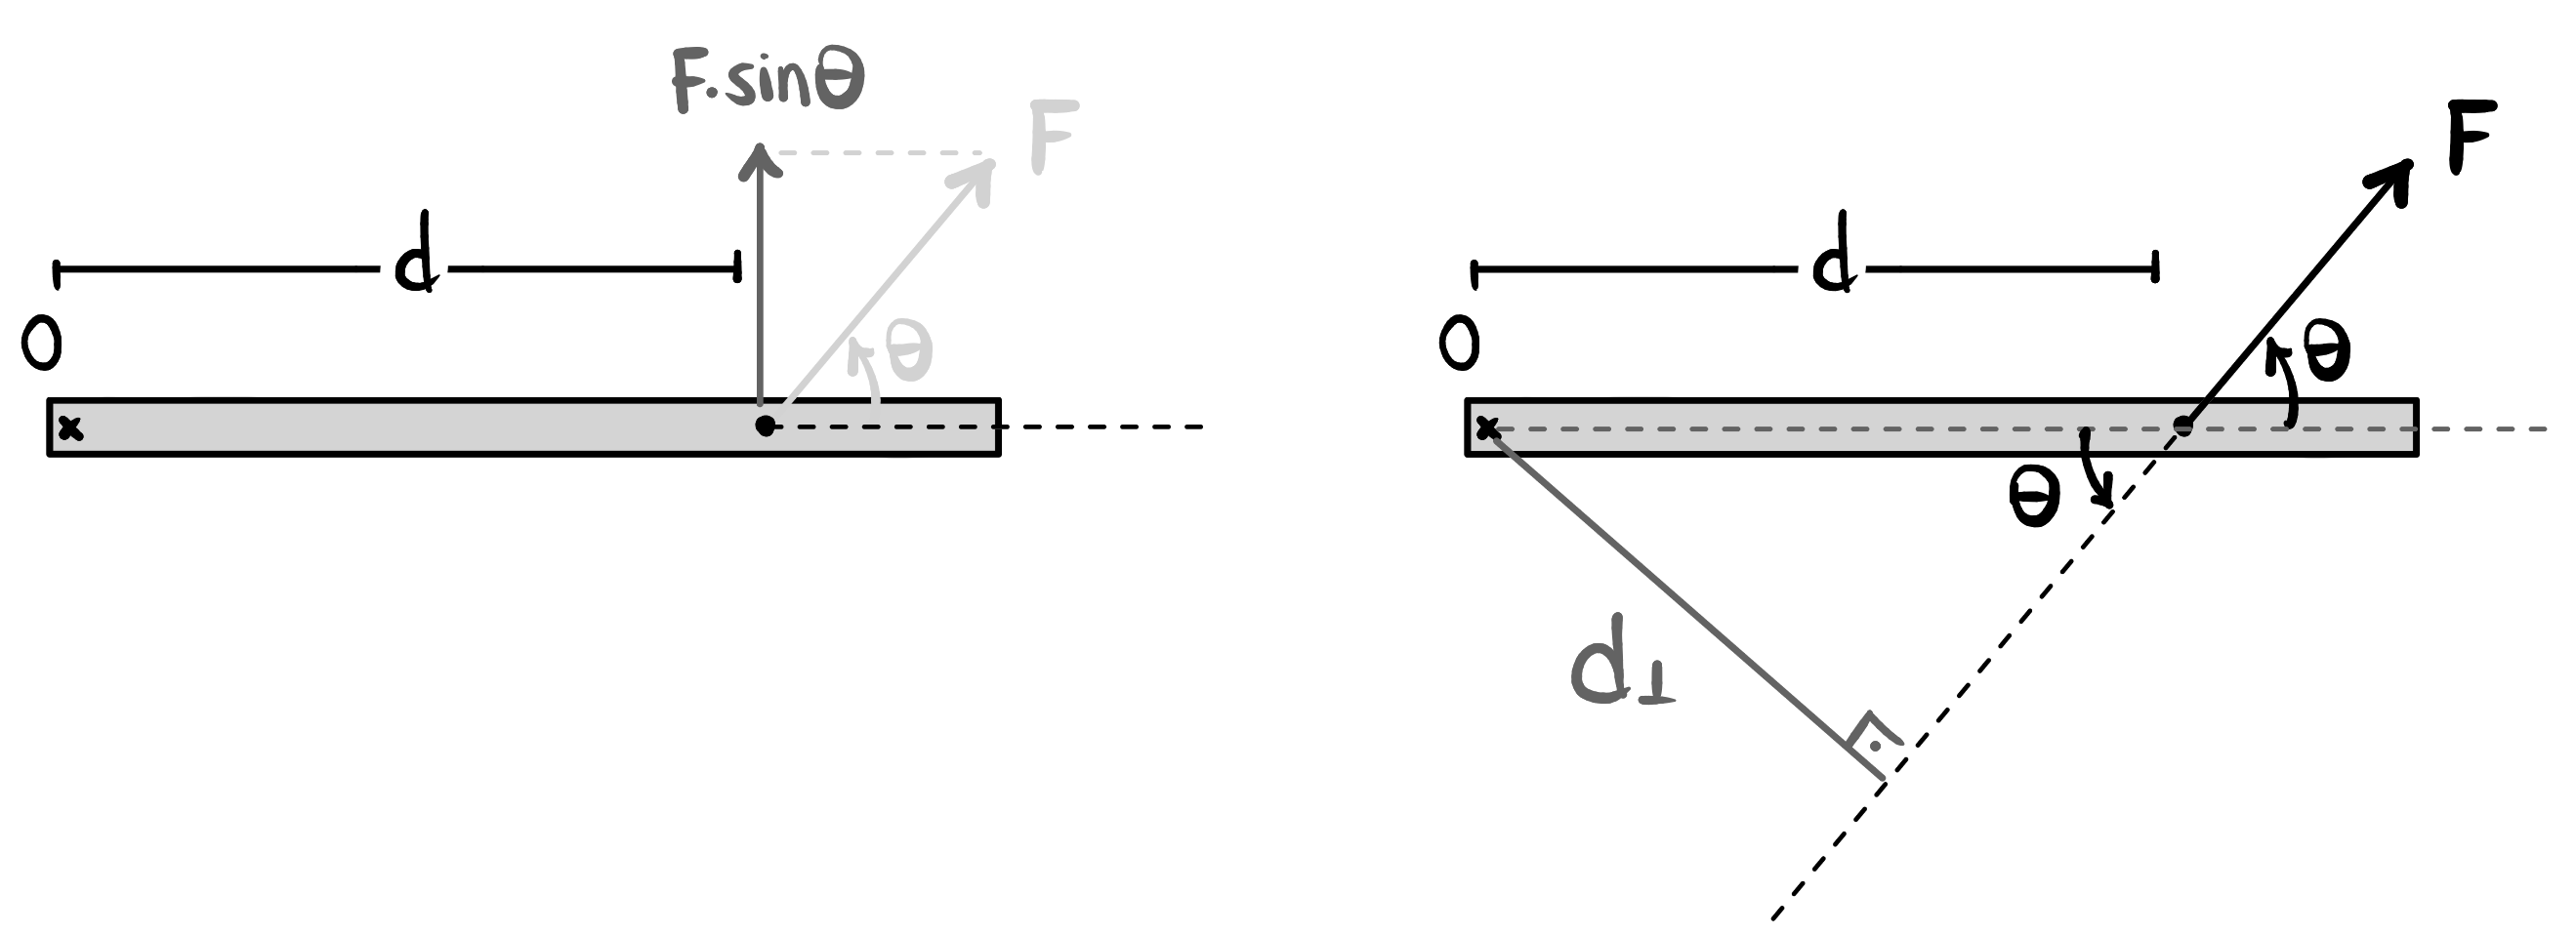
\includegraphics[width=0.8\linewidth]{imagensdinamicarotacao/torquedecompordistancia.png}};
  \end{scope}
\end{tikzpicture}
\captionof{figure}{O torque pode ser calculado decompondo a força ou a distância.}
\label{fig_dinamicarotacao_torque04}
} 
\vspace{0.3cm}

Observe a Figura \ref{fig_dinamicarotacao_torque04}. Do lado esquerdo temos a forma já apresentada para se computar o torque: dada uma força $F$, pegamos sua componente perpendicular à barra, no caso, a componente $F_{\perp} = F \sin \theta,$ e multiplicamos tal componente pela distância $d$ do ponto de aplicação da força $F$ até o ponto em relação ao qual estamos tomando os torques (ponto $O,$ no caso). 

Do lado direito da figura temos a construção que nos permite computar o torque da força $F$ em relação ao ponto $O$ de uma maneira alternativa. Neste caso, a força $F$ não é decomposta, ela fica exatamente como está. Traçamos a \textit{linha de ação da força $F$,} isto é, prolongamos o segmento de reta do vetor $\vec F.$ Feito isso, tomamos a distância da linha de ação da força $F$ até o ponto em relação ao qual estamos tomando os torques. Tal distância está representada por $d_{\perp}$ na figura. 

Feito isso, o torque da força $F$ em relação ao ponto $O$ será dado pelo produto da força $F$ (da forma como está, sem ser decomposta) pela distância $d_{\perp}$ da linha de ação da sua força até o ponto $O$, isto é:

$$ \tau = F \cdot d_{\perp} .$$

Isso pode ser provado por meio da aplicação da definição de seno no triângulo retângulo destacado do lado direito da Figura \ref{fig_dinamicarotacao_torque04}, de onde temos

$$ \sin \theta = \dfrac{d_{\perp}}{d} \implies d_{\perp} = d \sin \theta,$$

\noindent o que nos leva, na relação anterior, a 

$$ \tau = F \cdot d_{\perp} = F d \sin \theta,$$

\noindent que concorda com a Equação \eqref{eq_newton_torque}. Desse modo, estamos visualizando duas formas de interpretar tal equação:


$$\tau = \underbrace{(F \sin \theta)}_{\substack{\text{força} \\ \text{perpendicular}}} \cdot d \quad = \quad F \cdot \underbrace{(d \sin \theta)}_{\substack{\text{distância} \\ \text{perpendicular}}}$$

Na primeira situação, a distância é mantida fixa, e toma-se a componente da força perpendicular a tal distância. Já na segunda, a força é mantida fixa, e toma-se a distância de tal força (da sua linha de ação, no caso) até o ponto em relação ao qual calcula-se os torques.

A fim de trazer clareza uma situação em que é mais útil decompor distâncias do que forças, considere a situação em que uma escada homogênea de massa $m = 20$ kg e comprimento $L=20$ metros está apoiada em uma parede vertical, fazendo um ângulo de $30^\circ$ com a horizontal. Um pedreiro de massa $M=80$ kg sobe pela escada e para quando está a $\sfrac{3}{5}$ do comprimento dela\footnote{Estamos considerando que não existe atrito entre a escada e a parede vertical.}. 


{
\centering
\begin{tikzpicture}
  \begin{scope}[blend mode=multiply]
    \node {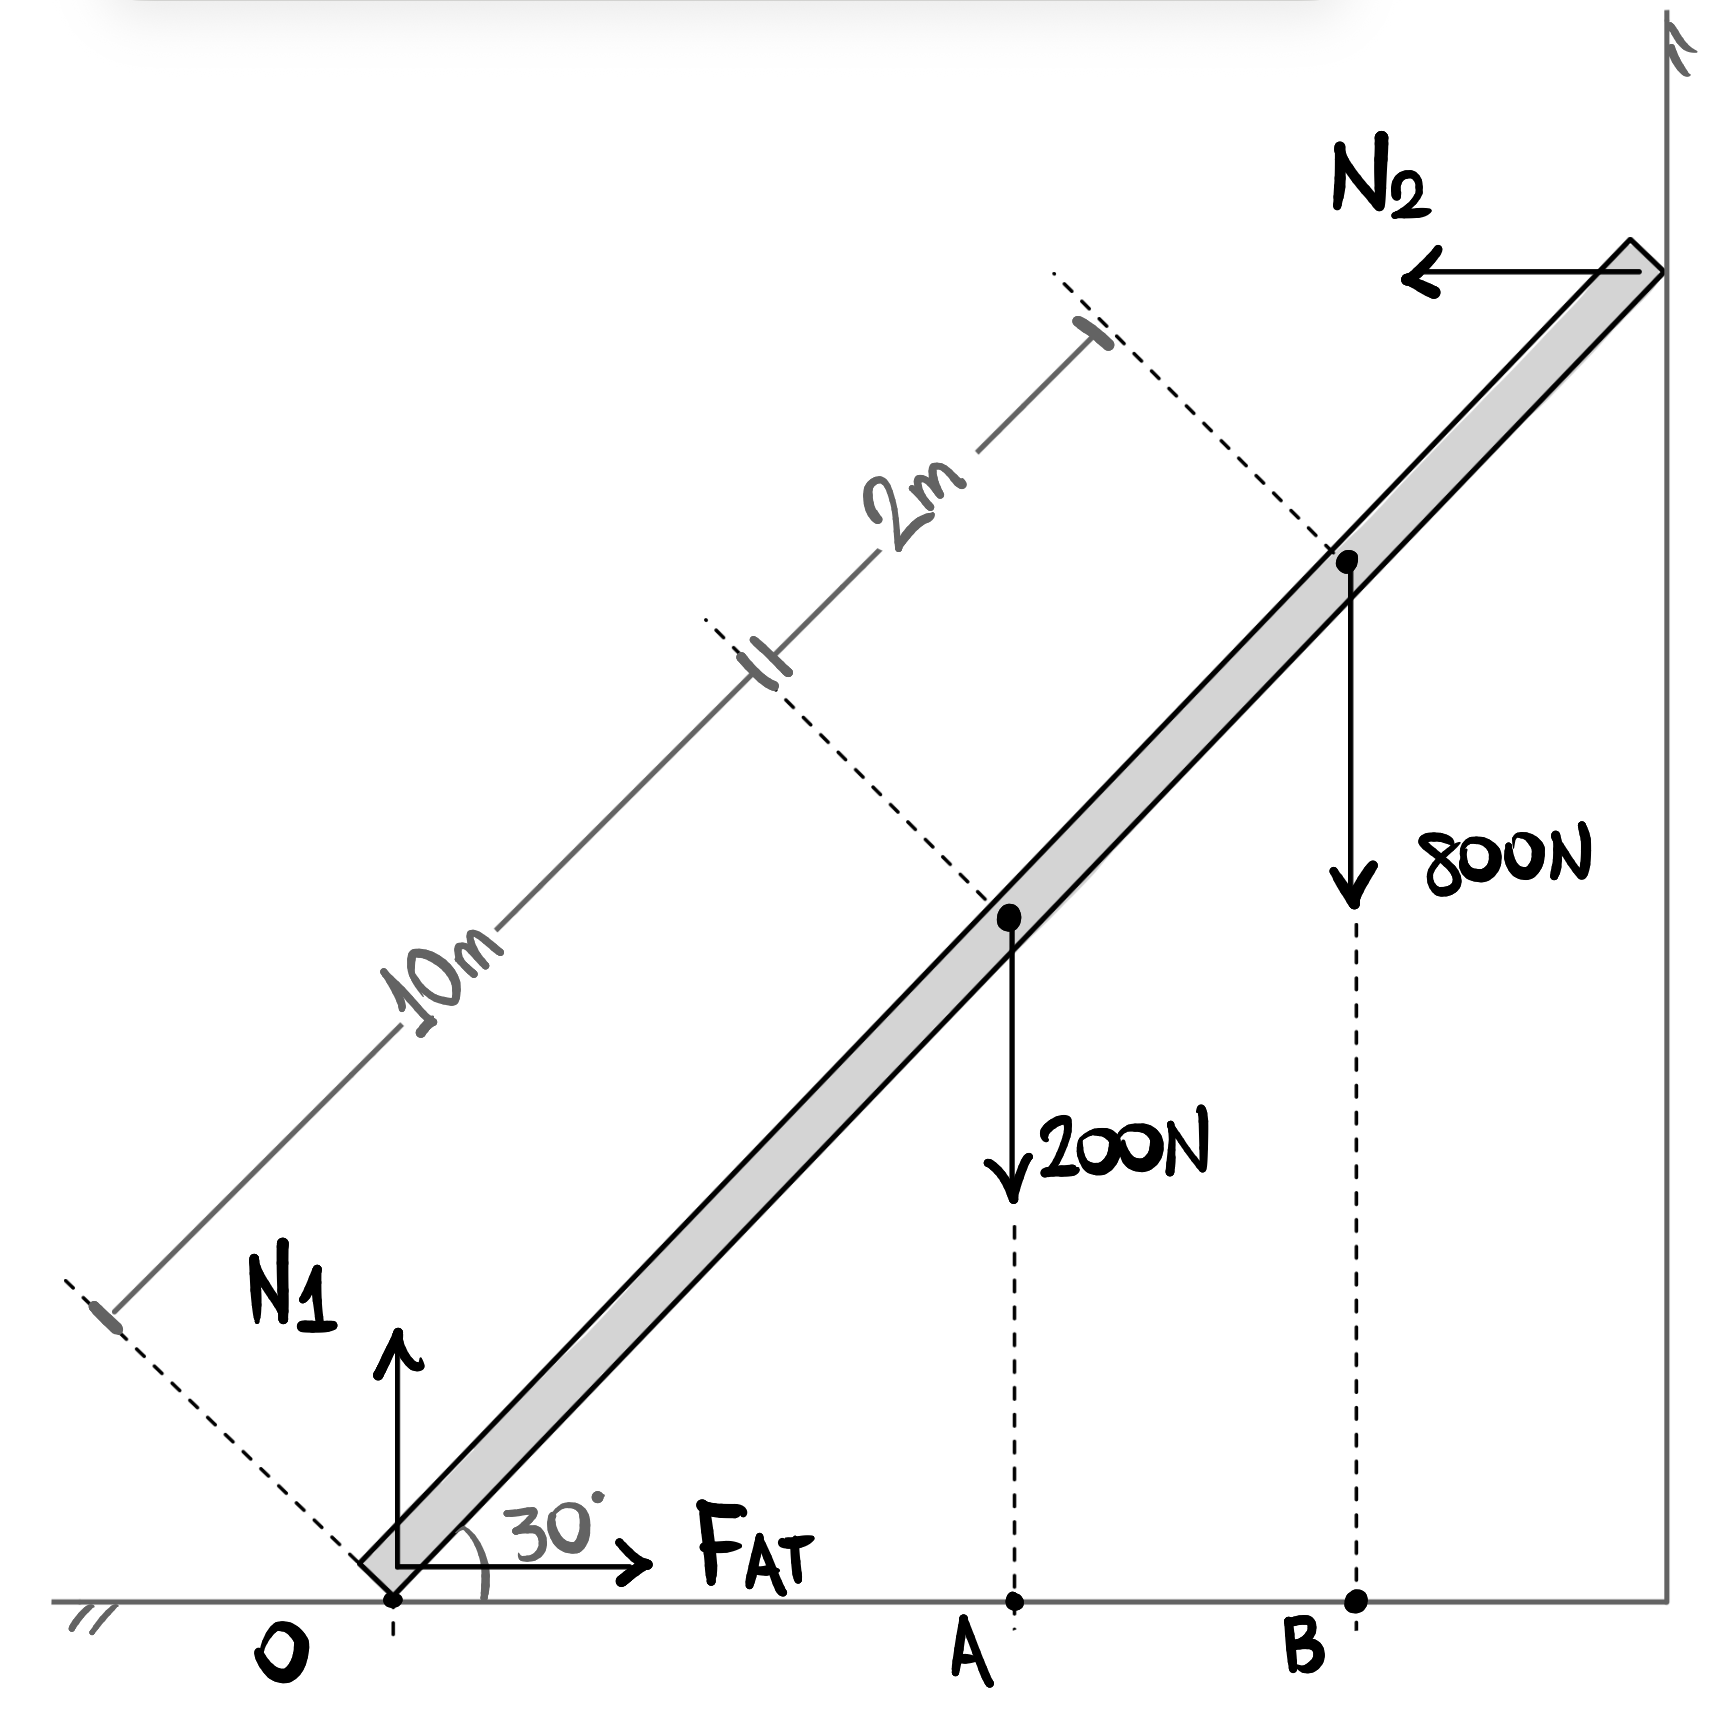
\includegraphics[width=0.4\linewidth]{imagensdinamicarotacao/torqueescada.png}};
  \end{scope}
\end{tikzpicture}
\captionof{figure}{Forças e torques em uma escada.}
\label{fig_dinamicarotacao_torqueescada}
} 
\vspace{0.3cm}


Considere o problema de calcular o valor da força de atrito que o piso exerce sob a base da escada nessa situação, considerando que o sistema está em equilíbrio. A Figura \ref{fig_dinamicarotacao_torqueescada} mostra o diagrama de forças na escada. O pedreiro subiu $\sfrac{3}{5}$ da escada, o que, para 20 metros, equivale a 12 metros de subida. 

Tomando os torques em relação ao ponto $O$, as forças $N_1$ e $F_\text{AT}$, feitas pelo chão sob a barra, não gerarão torque. Os torques devido aos pesos, neste caso, tendem a girar a barra no sentido horário, enquanto o torque da normal $N_2$ feita pela parede na barra tende a girá-la no sentido anti-horário. Equacionando o equilíbrio, teremos

$$ \tau_{\text{R}_\text{O}} = 0 \implies N_2 \cdot h = 200 \cdot \overline{OA} + 800 \cdot \overline{OB}.$$

Note que, neste caso, para computar os torques, optamos por não decompor as forças. Deixamos elas como estavam, e as multiplicamos pelas respectivas distâncias de suas linhas de ação ao ponto em relação ao qual tomamos os torques. Essas distâncias podem ser relacionadas por trigonometria simples ($h$ é a distância do ponto de apoio da barra na parede vertical até o chão), como segue:

$$ \cos 30^\circ = \dfrac{\overline{OA}}{10} \implies \boxed{\overline{OA}= 5\sqrt 3.} \quad \text{ e } \quad \cos 30^\circ = \dfrac{\overline{OB}}{12} \implies \boxed{\overline{OB}= 6\sqrt 3.}$$

Usando agora o seno no triângulo retângulo maior, temos


$$ \sin 30^\circ = \dfrac{h}{20} \implies \boxed{h = 10.}$$

Assim, usando tais valores na equação de equilíbrio dos torques, teremos

$$  N_2 \cdot 10 = 200 \cdot 5 \sqrt 3 + 800 \cdot 6 \sqrt 3 \implies \boxed{N_2 =580 \sqrt 3 \text{ N.} }$$

Impondo agora o equilíbrio de forças, teremos

$$ \vec F_\text{R} = 0 \begin{cases}
    F_\text{x} = 0 \implies F_\text{AT} = N_2 \implies \boxed{F_\text{AT} =580 \sqrt 3 \text{ N.} }  \\   
    \rule{0pt}{1.5em} F_\text{y} = 0 \implies N_1 = 200 + 800 \implies \boxed{N_1 = 1.000 \text{ N} ,}\\
\end{cases}$$

\noindent de modo que foi possível encontrar todas as forças que atuam na barra: o atrito e as duas normais feitas pelo chão e pela parede.

\vspace{0.3cm}


\begin{exemplo}[Nível I]\label{exemplo_newton_torqueex01}

A Figura \ref{fig_dinamicarotacao_torqueexemplo01} mostra uma balança de gangorra, de massa desprezível, e com o apoio fixado em seu centro. As crianças possuem massas $m_\text{A}=35$ kg e $m_{\text{B}} = 50$ kg, o comprimento da barra da gangorra é de 10 metros. Nessa situação, a balança está em equilíbrio?

\vspace{0.3cm}
{
\centering
\begin{tikzpicture}
  \begin{scope}[blend mode=multiply]
    \node {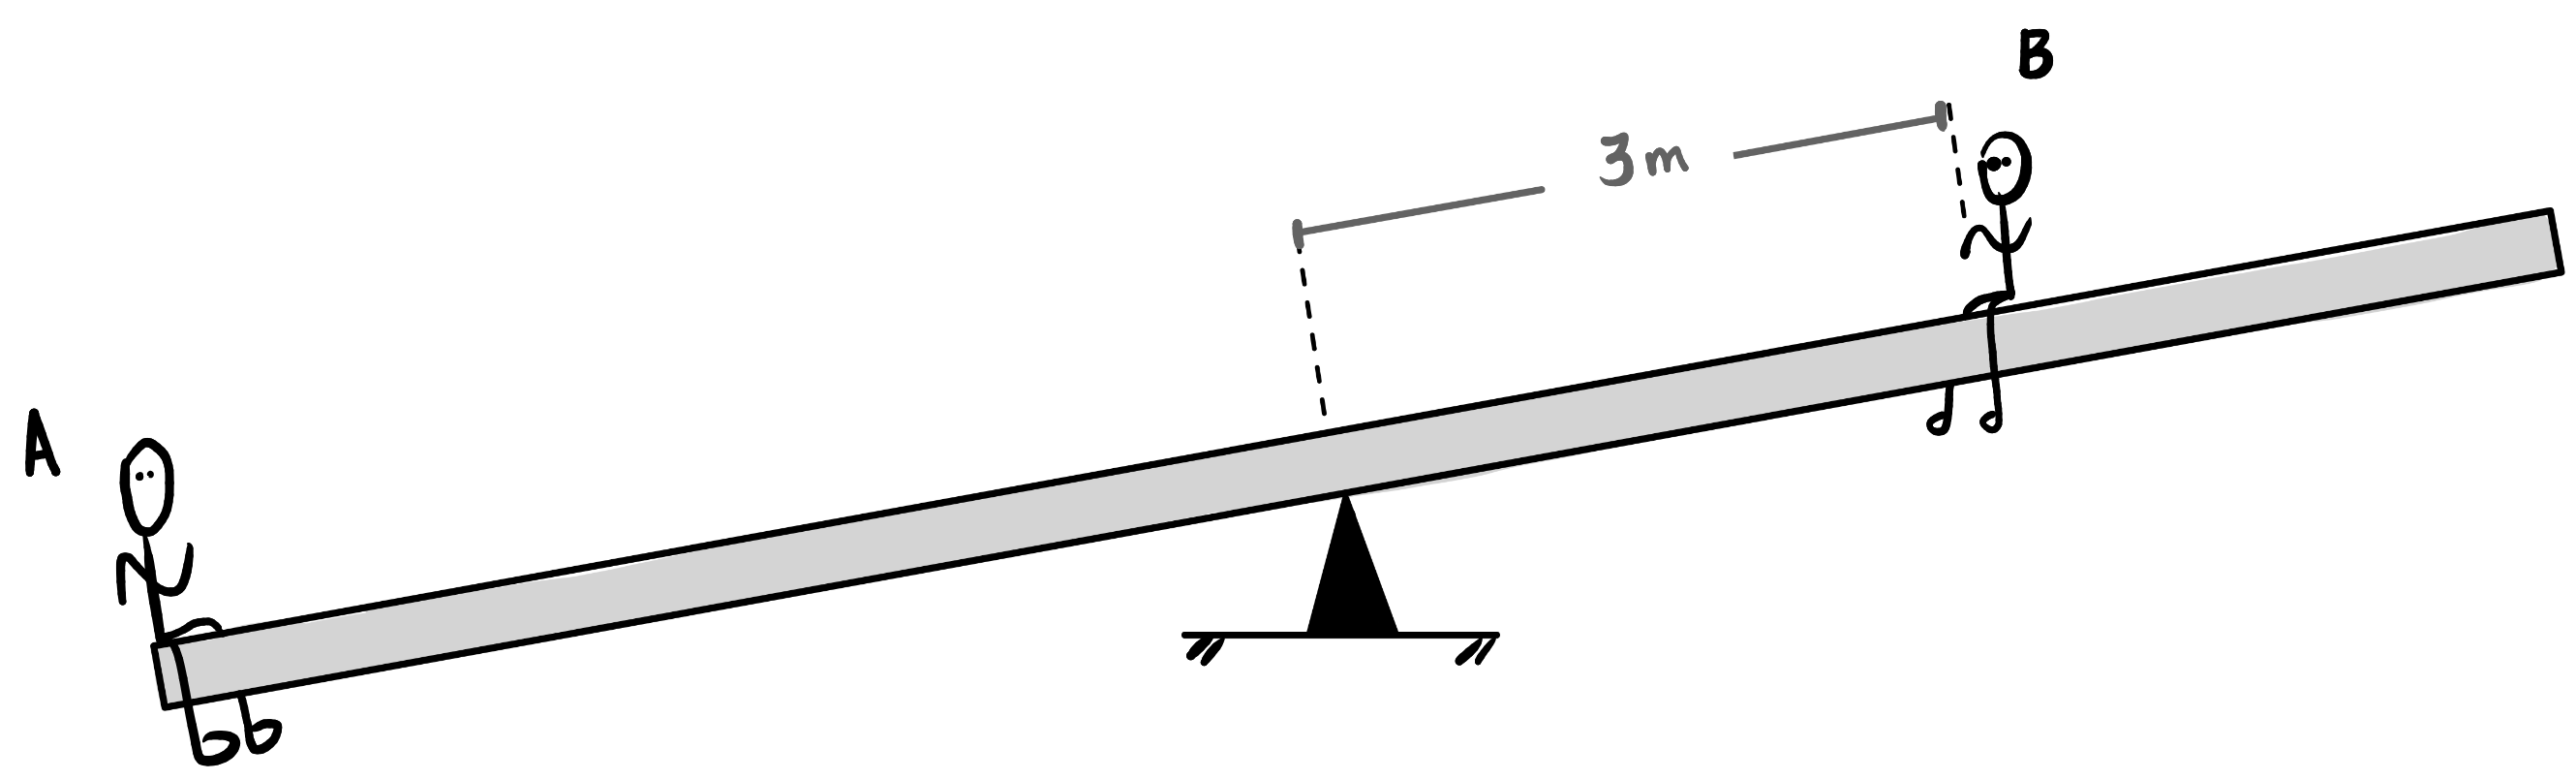
\includegraphics[width=0.6\linewidth]{imagensdinamicarotacao/torqueexemplo011.png}};
  \end{scope}
\end{tikzpicture}
\captionof{figure}{}
\label{fig_dinamicarotacao_torqueexemplo01}
} 
\vspace{0.3cm}

\resolucao

A Figura \ref{fig_dinamicarotacao_torqueexemplo012} mostra o diagrama de forças atuando na barra (lembre-se que a força normal -- trocada entre o menino e a barra -- é sempre perpendicular à superfície de contato)\footnote{A rigor, a força normal seria igual à componente $P_y=P \cos \theta$ do peso de cada garoto, exatamente como um plano inclinado. Contudo, sendo $\theta$ o mesmo ângulo, o cosseno irá aparecer tanto para a força trocada entre o garoto $A$ e a barra quanto para o garoto $B$ e a barra, de modo que ele cancelaria na hora que igualássemos os torques.}. 

\vspace{0.3cm}
{
\centering
\begin{tikzpicture}
  \begin{scope}[blend mode=multiply]
    \node {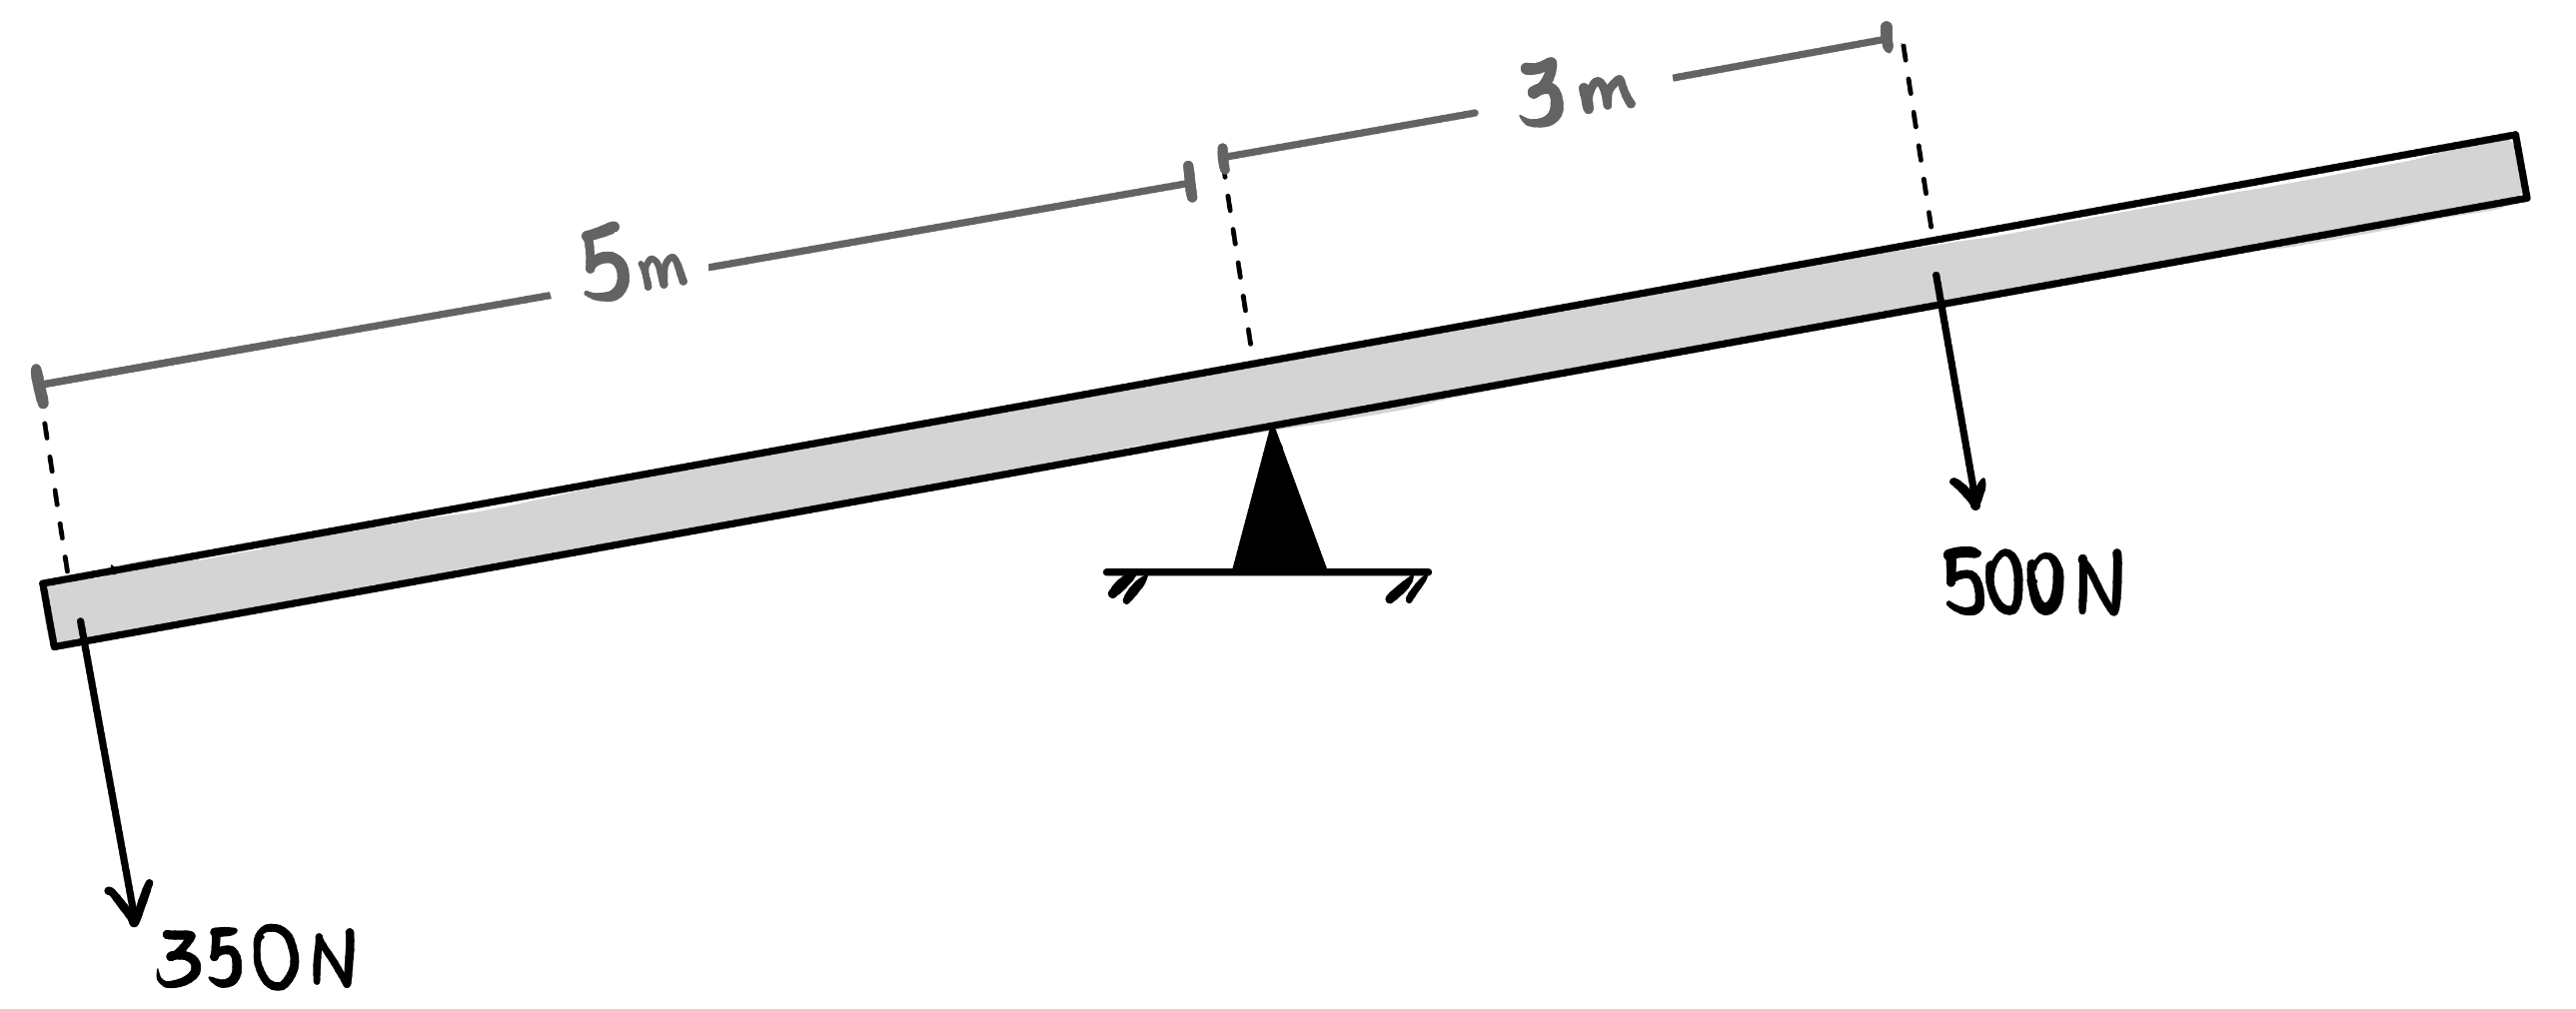
\includegraphics[width=0.6\linewidth]{imagensdinamicarotacao/torqueexemplo012.png}};
  \end{scope}
\end{tikzpicture}
\captionof{figure}{}
\label{fig_dinamicarotacao_torqueexemplo012}
} 
\vspace{0.3cm}

Vemos que, devido ao peso do menino $A$, existe um torque, em relação ao centro da barra, que vale $\tau_\text{A} = 350 \cdot 5 = 1.750 \text{ N $\cdot$ m},$ no sentido anti-horário. Adotando tal sentido como negativo, teríamos na verdade  $\tau_\text{A} = -1.750 \text{ N $\cdot$ m}.$


Já o torque gerado devido à criança $B$ tende a girar a barra no sentido horário, sendo, portanto, positivo na nossa convenção. Tal torque vale  $\tau_\text{B} = 500 \cdot 3 = 1.500 \text{ N $\cdot$ m},$ de modo que o torque resultante em relação ao centro da barra é

$$ \tau_\text{R} = \tau_\text{A} + \tau_\text{B} = -1.750 + 1500 = -250 \text{ N $\cdot$ m}, $$

\noindent ou seja, como $\tau_\text{R} \neq 0$, a barra não está em equilíbrio. Sendo o torque resultante negativo, sabemos que ela gira no sentido anti-horário, ou seja, o torque gerado devido ao peso do menino $A$ -- mesmo este sendo mais leve que o $B$ -- é maior. Isso ocorre porque, apesar de ser mais leve, a criança $A$ está afastada o suficiente do centro da barra de modo a compensar seu menor peso e, ainda assim, gerar um torque superior, por ter um braço de alavanca maior.

\end{exemplo}


\vspace{0.3cm}



\begin{exemplo}[Nível II]\label{exemplo_newton_torqueex02}

Considere a situação da Figura \ref{fig_dinamicarotacao_torque2apoios}, em que massa da esquerda vale $m=5$ kg e está a 2 metros da extremidade esquerda da barra. A massa da direita vale $m= 2$ kg e está a 2 metros da extremidade direita da barra.

Se a barra é homogênea, possui um comprimento de 10 metros e massa de 3 kg, calcule as forças de contato que os apoios fazem na barra.


\resolucao

A Figura \ref{fig_dinamicarotacao_torque2apoiosexemplo} mostra o diagrama das forças que atuam na barra. Tomando os torques em relação ao ponto $A,$ vemos a única força que irá gerar um torque no sentido anti-horário será a normal no apoio $B,$ todas as outras gerarão torques no sentido horário. Equacionado o equilíbrio, teremos:

$$\tau_{\text{R}_{A}} = 0 \implies N_\text{B} \cdot 10 = 20 \cdot 8 + 30 \cdot 5 +50 \cdot 2 \implies \boxed{N_\text{B} = 41 \text{ N}.} $$


\vspace{0.3cm}
{
\centering
\begin{tikzpicture}
  \begin{scope}[blend mode=multiply]
    \node {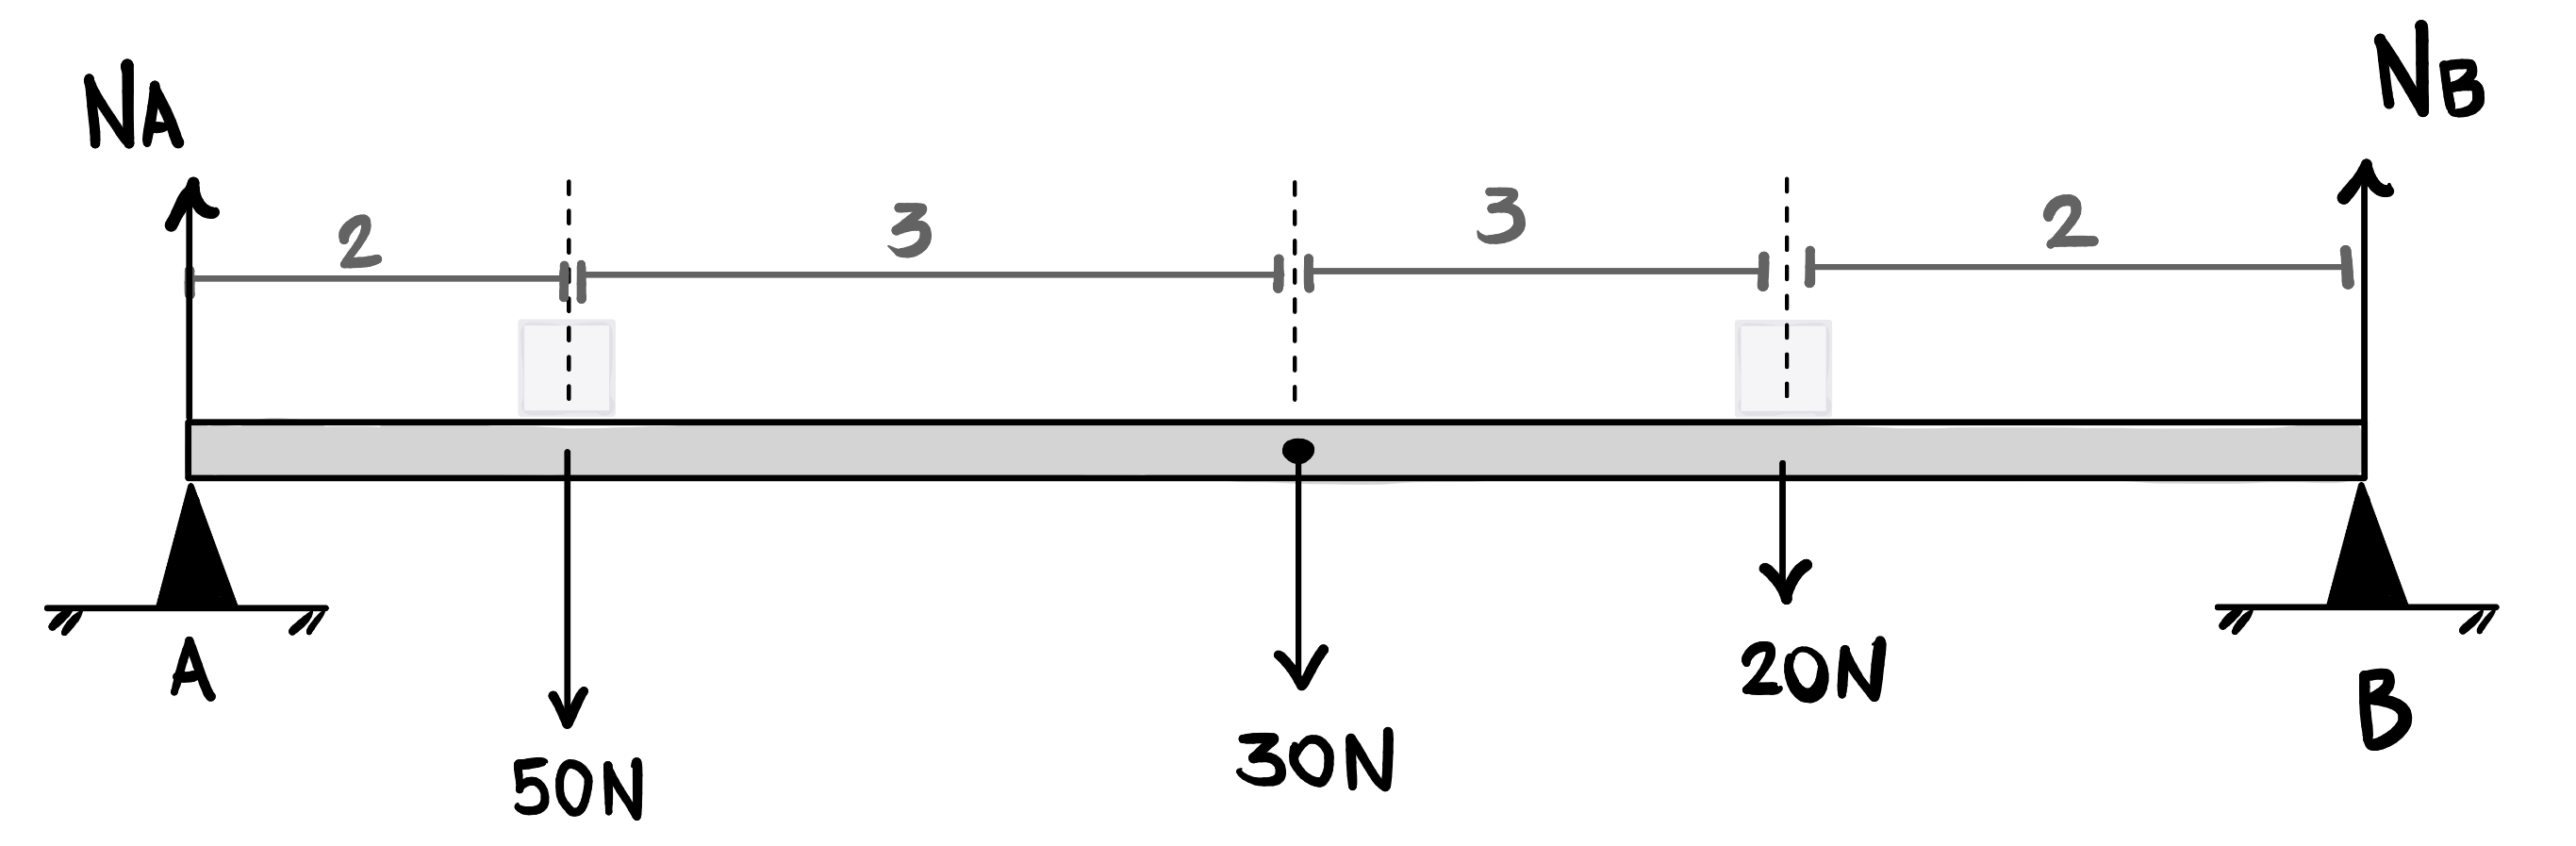
\includegraphics[width=0.7\linewidth]{imagensdinamicarotacao/torqueexemplo2apoios.png}};
  \end{scope}
\end{tikzpicture}
\captionof{figure}{}
\label{fig_dinamicarotacao_torque2apoiosexemplo}
} 
\vspace{0.3cm}

Impondo agora a condição de equilíbrio de translação, isto é, a barra não acelera verticalmente, teremos

$$ F_{\text{R}_{y}} = 0 \implies N_\text{A} + N_\text{B} = 50 + 30 + 20 \implies N_\text{A} + 41 = 100 \implies \boxed{N_\text{A} = 59 \text{ N}.} $$

Fica a reflexão para leitor: por qual motivo a normal no apoio esquerdo é maior do que no direito? Poderíamos prever isso, antes mesmo de fazer os cálculos? Além disso, refaça o exercício, do zero, tomando como pivô o ponto $B,$ depois tomando como pivô o centro da barra. Os resultados concordaram?

\end{exemplo}

\vspace{0.3cm}


\begin{exemplo}[Nível III - (ITA 2009)]\label{exemplo_newton_torqueex03}




Chapas retangulares rígidas, iguais e homogêneas, são sobrepostas e deslocadas entre si, formando um conjunto que se apoia parcialmente na borda de uma calçada. A figura ilustra esse conjunto com $n$ chapas, bem como a distância $D$ alcançada pela sua parte suspensa.

\vspace{0.3cm}

\begin{center}
\begin{tikzpicture}[scale=0.6]

    % Parâmetros
    \def\L{6.0}
    \def\h{0.28}
    \def\dx{0.7}
    \def\n{6}
    \def\xedge{3.5} % borda da calçada

    % Superfície horizontal à esquerda
    \draw[thick] (-2.8,0) -- (\xedge,0);

    % Hachuras da superfície horizontal
    \foreach \x in {-2.6,-2.2,-1.8,-1.4,-1.0,-0.6,-0.2,0.2,0.6,1.0,1.4,1.8,2.2,2.6,3.0} {
        \draw[thin] (\x,0) -- ++(-0.15,-0.35);
    }

    % Face vertical da calçada
    \draw[thick] (\xedge,0) -- (\xedge,-2.3);

    % Hachuras da face vertical
    \foreach \y in {-0.2,-0.6,-1.0,-1.4,-1.8,-2.2} {
        \draw[thin] (\xedge,\y) -- ++(-0.22,-0.18);
    }

    % Chapas empilhadas
    \foreach \i in {0,1,2,3,4,5} {
        \pgfmathsetmacro{\xstart}{0.4+\i*\dx}
        \pgfmathsetmacro{\ystart}{\i*\h}
        \draw[thick, fill=gray!10] (\xstart,\ystart) rectangle ++(\L,\h);
    }

    % Linha tracejada vertical na extremidade direita
    \draw[densely dotted, thick] ({0.4+5*\dx+\L},0) -- ({0.4+5*\dx+\L},2.25);

    % Cota L
    \draw[thin] ({0.4+5*\dx},2.0) -- ({0.4+5*\dx},2.35);
    \draw[thin] ({0.4+5*\dx+\L},2.0) -- ({0.4+5*\dx+\L},2.35);
    \draw[thin] ({0.4+5*\dx},2.2) -- ({0.4+5*\dx+\L},2.2);
    \node at ({0.4+5*\dx+\L/2},2.55) {$L$};

    % Cota D
    \draw[thin] (\xedge,-1.5) -- ({0.4+5*\dx+\L},-1.5);
    \draw[thin] (\xedge,0.1) -- (\xedge,-1.65);
    \draw[thin] ({0.4+5*\dx+\L},0.1) -- ({0.4+5*\dx+\L},-1.65);
    \node at ({(\xedge+0.4+5*\dx+\L)/2},-1.95) {$D$};

\end{tikzpicture}
\end{center}

\vspace{0.3cm}

Desenvolva uma fórmula geral da máxima distância $D$ possível de modo que o conjunto ainda se mantenha em equilíbrio. A seguir, calcule essa distância $D$ em função do comprimento $L$ de cada chapa, para $n = 6$ unidades.


\resolucao

Considere as barras $1,2,3, \dots, n$ sendo contadas a partir da barra superior. Sejam $x_1,x_2,x_3, \dots x_n$ as distâncias que cada barra avança em relação à extremidade da barra debaixo, como ilustra a Figura \ref{fig_dinamicarotacao_itaexemplotorquepilhadebarras1}. A distância pedida é o somatório desses avanços, isto é:

$$ D = x_1 + x_2 + x_3 + \dots + x_n = \sum_{k=1}^n x_k.$$



\vspace{0.3cm}
{
\centering
\begin{tikzpicture}
  \begin{scope}[blend mode=multiply]
    \node {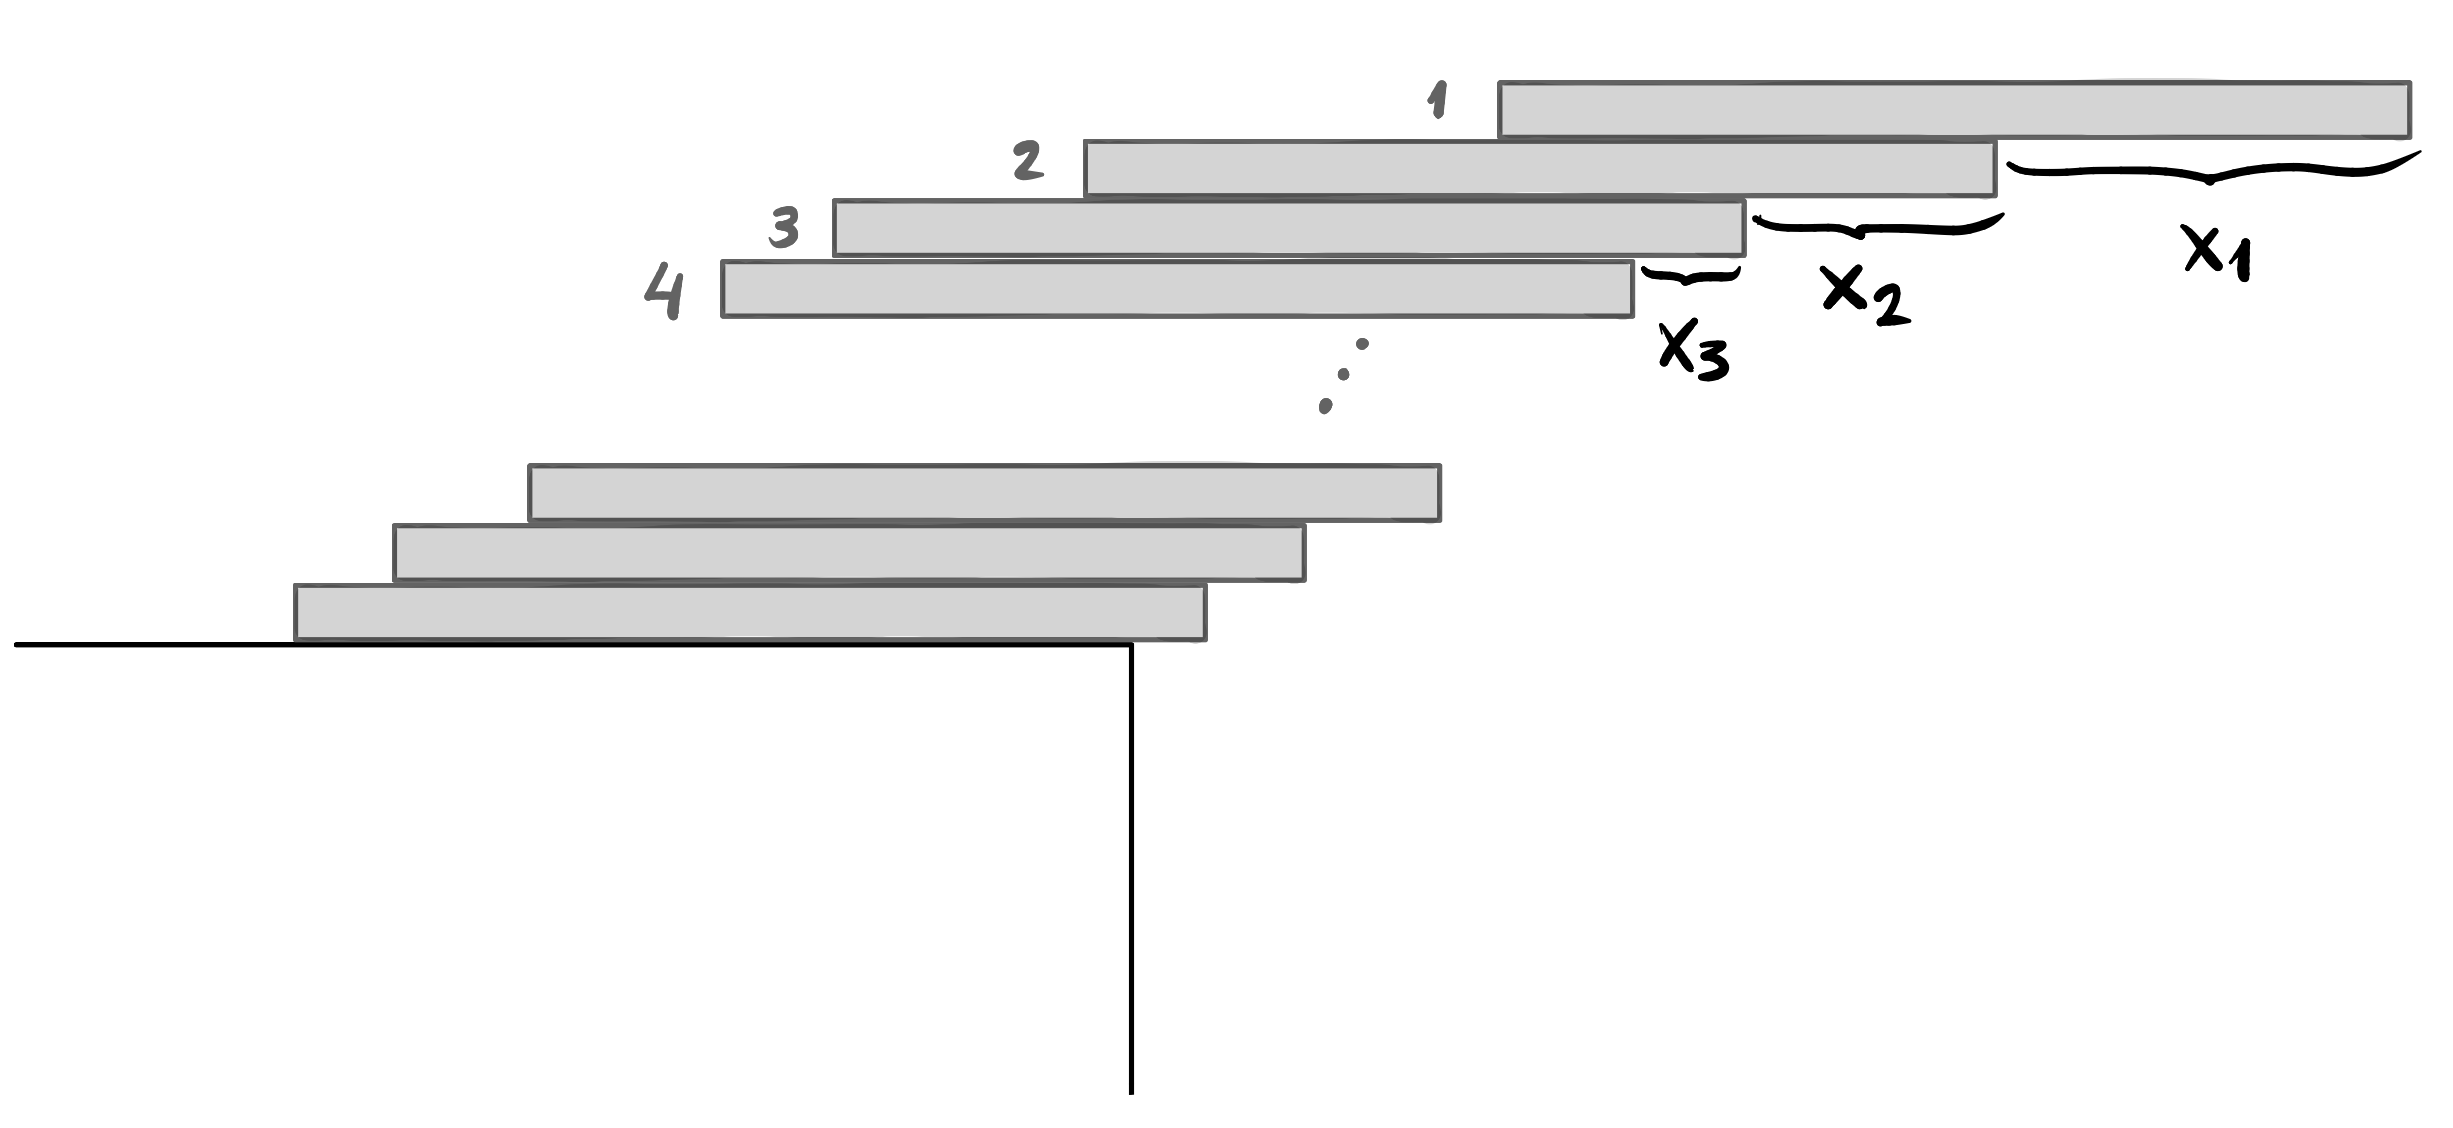
\includegraphics[width=0.6\linewidth]{imagensdinamicarotacao/itaexemplotorquepilhadebarras1.png}};
  \end{scope}
\end{tikzpicture}
\captionof{figure}{}
\label{fig_dinamicarotacao_itaexemplotorquepilhadebarras1}
} 
\vspace{0.3cm}


Avaliemos inicialmente o contato entre as barras 1 e 2, como mostra a Figura \ref{fig_dinamicarotacao_itaexemplotorquepilhadebarras2}. Consideremos que a barra 1 está na iminência de tombamento, ou seja, se empurrada um pouquinho a mais para direita ela tombaria. Logo, seu contato com a barra debaixo está todo concentrado na extremidade da barra 2, com o seu centro de massa exatamente neste ponto de contato.


\vspace{0.3cm}
{
\centering
\begin{tikzpicture}
  \begin{scope}[blend mode=multiply]
    \node {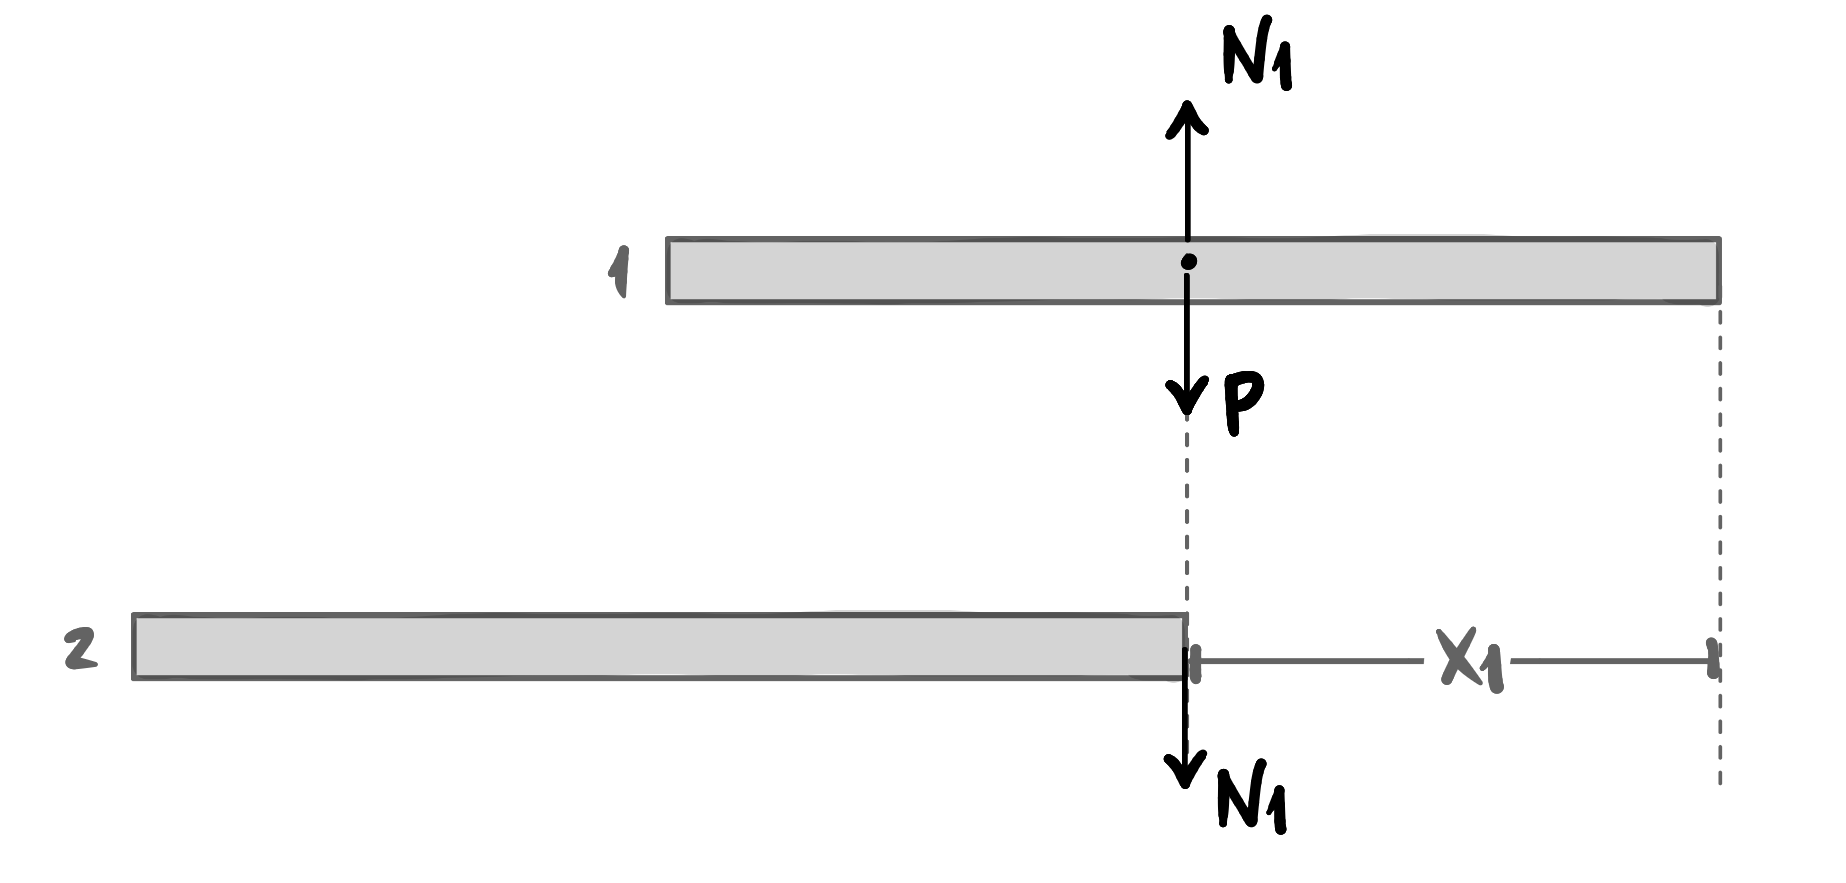
\includegraphics[width=0.45\linewidth]{imagensdinamicarotacao/itaexemplotorquepilhadebarras2.png}};
  \end{scope}
\end{tikzpicture}
\captionof{figure}{Forças nas barras 1 e 2.}
\label{fig_dinamicarotacao_itaexemplotorquepilhadebarras2}
} 
\vspace{0.3cm}

Se o centro de massa da barra 1 estiver à direita da extremidade da barra 2 então ela tombaria. Considerando o centro de massa exatamente alinhado com a extremidade estamos na situação limite. Logo, neste caso, teremos

$$ \boxed{ x_1 = \dfrac{L}{2}.}$$

Naturalmente temos, do equilíbrio da barra $1,$ que $N_1 = P.$ Avaliando agora as forças na barra 2, teremos agora 3 forças atuando nela: a normal $N_1$ trocada com a barra 1, seu peso $P$ e a normal $N_2$ trocada com a barra 3. A Figura \ref{fig_dinamicarotacao_itaexemplotorquepilhadebarras3} mostra esse diagrama de forças. 


\vspace{0.3cm}
{
\centering
\begin{tikzpicture}
  \begin{scope}[blend mode=multiply]
    \node {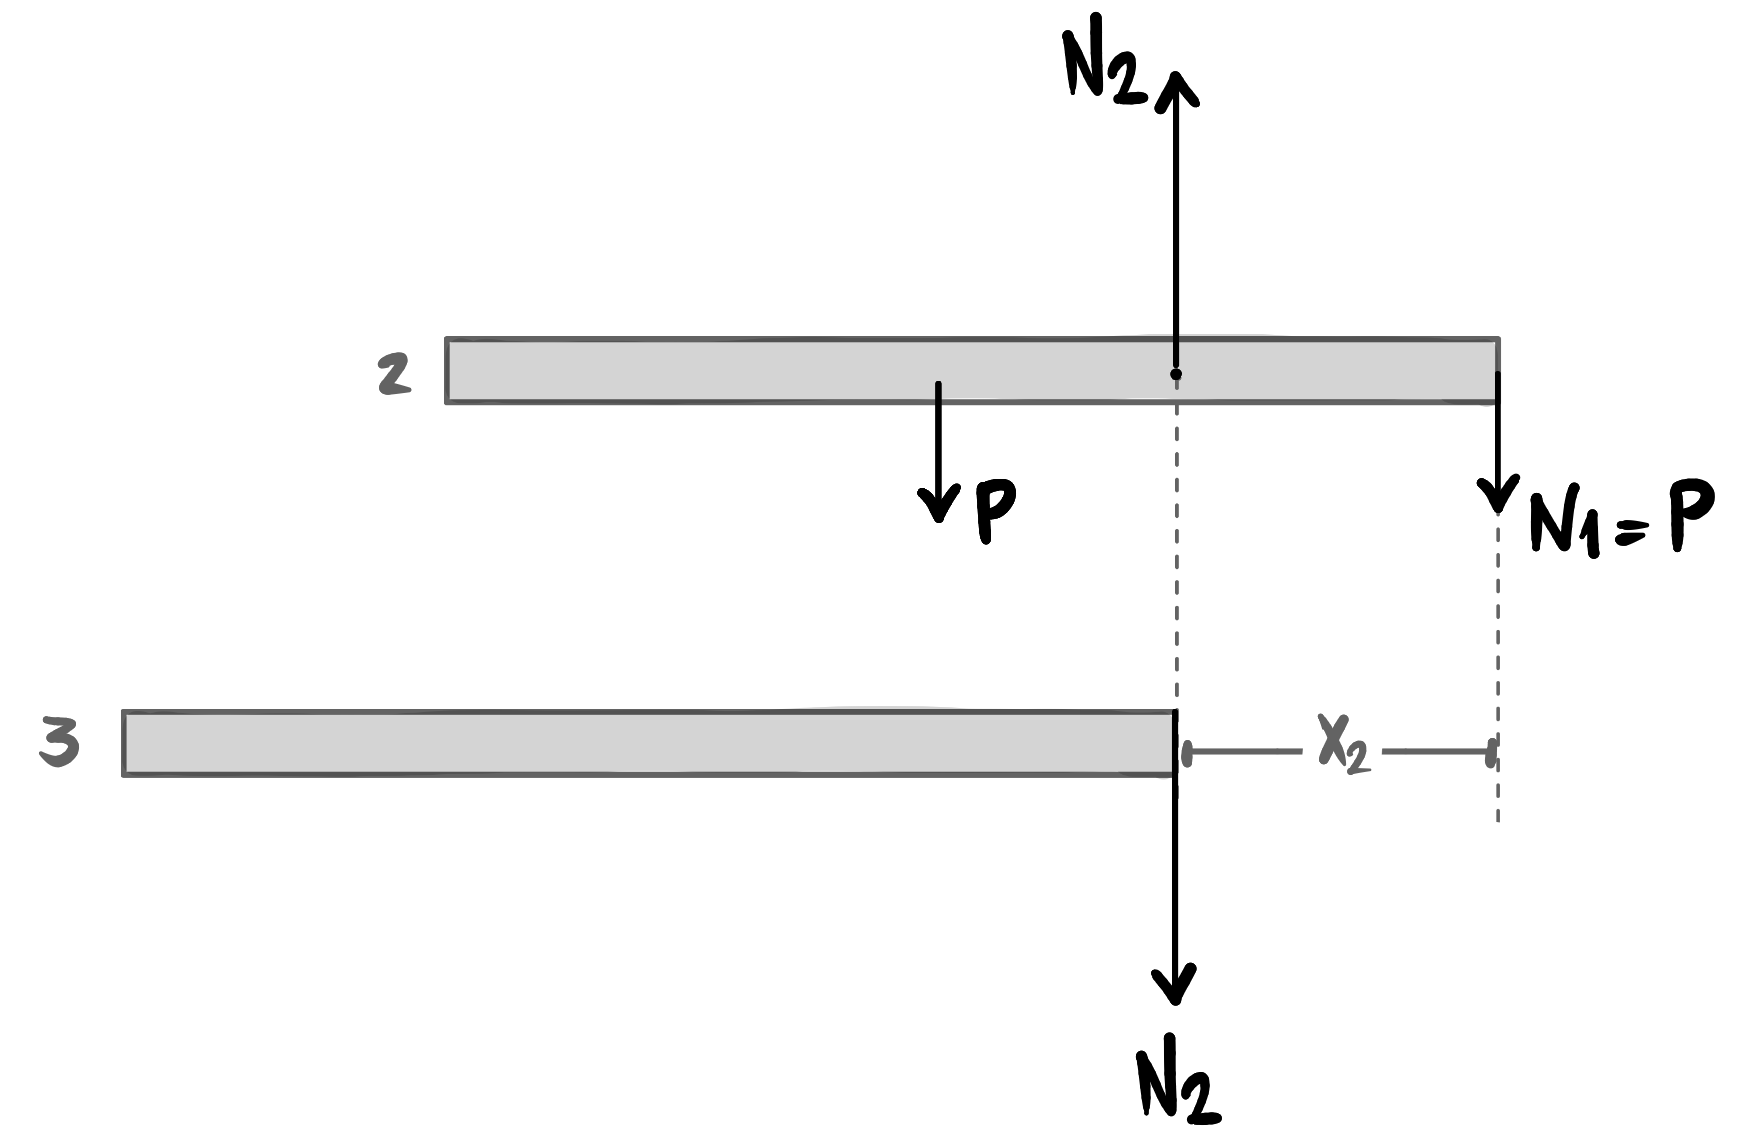
\includegraphics[width=0.45\linewidth]{imagensdinamicarotacao/itaexemplotorquepilhadebarras3.png}};
  \end{scope}
\end{tikzpicture}
\captionof{figure}{Forças nas barras 2 e 3.}
\label{fig_dinamicarotacao_itaexemplotorquepilhadebarras3}
} 
\vspace{0.3cm}

Quando consideramos a normal $N_2$ atuando exatamente no ponto alinhado com a extremidade da barra debaixo estamos dizendo que a barra de cima está na iminência de tombar: sua extremidade esquerda está praticamente levantada, estando o contato concentrado em um único ponto -- a extremidade da barra debaixo. Assim, estando na iminência de tombar, estaremos considerando o caso limite. Do equilíbrio de torques da barra 2 (em relação ao ponto em que atua a força $N_2$) teremos:

$$ \tau_R = 0 \implies N_1 \cdot x_2 = P \cdot \left( \dfrac{L}{2} - x_2 \right) \implies  \cancel P \cdot x_2 = \cancel P \cdot \left( \dfrac{L}{2} - x_2 \right) \implies \boxed{x_2= \dfrac{L}{4}.}   $$

Naturalmente, do equilíbrio de forças na barra 2, teremos $N_2 = P + N_1 =2P.$
\medskip
Considerando agora as forças na barra 3, observe a Figura \ref{fig_dinamicarotacao_itaexemplotorquepilhadebarras4}. 

\vspace{0.3cm}
{
\centering
\begin{tikzpicture}
  \begin{scope}[blend mode=multiply]
    \node {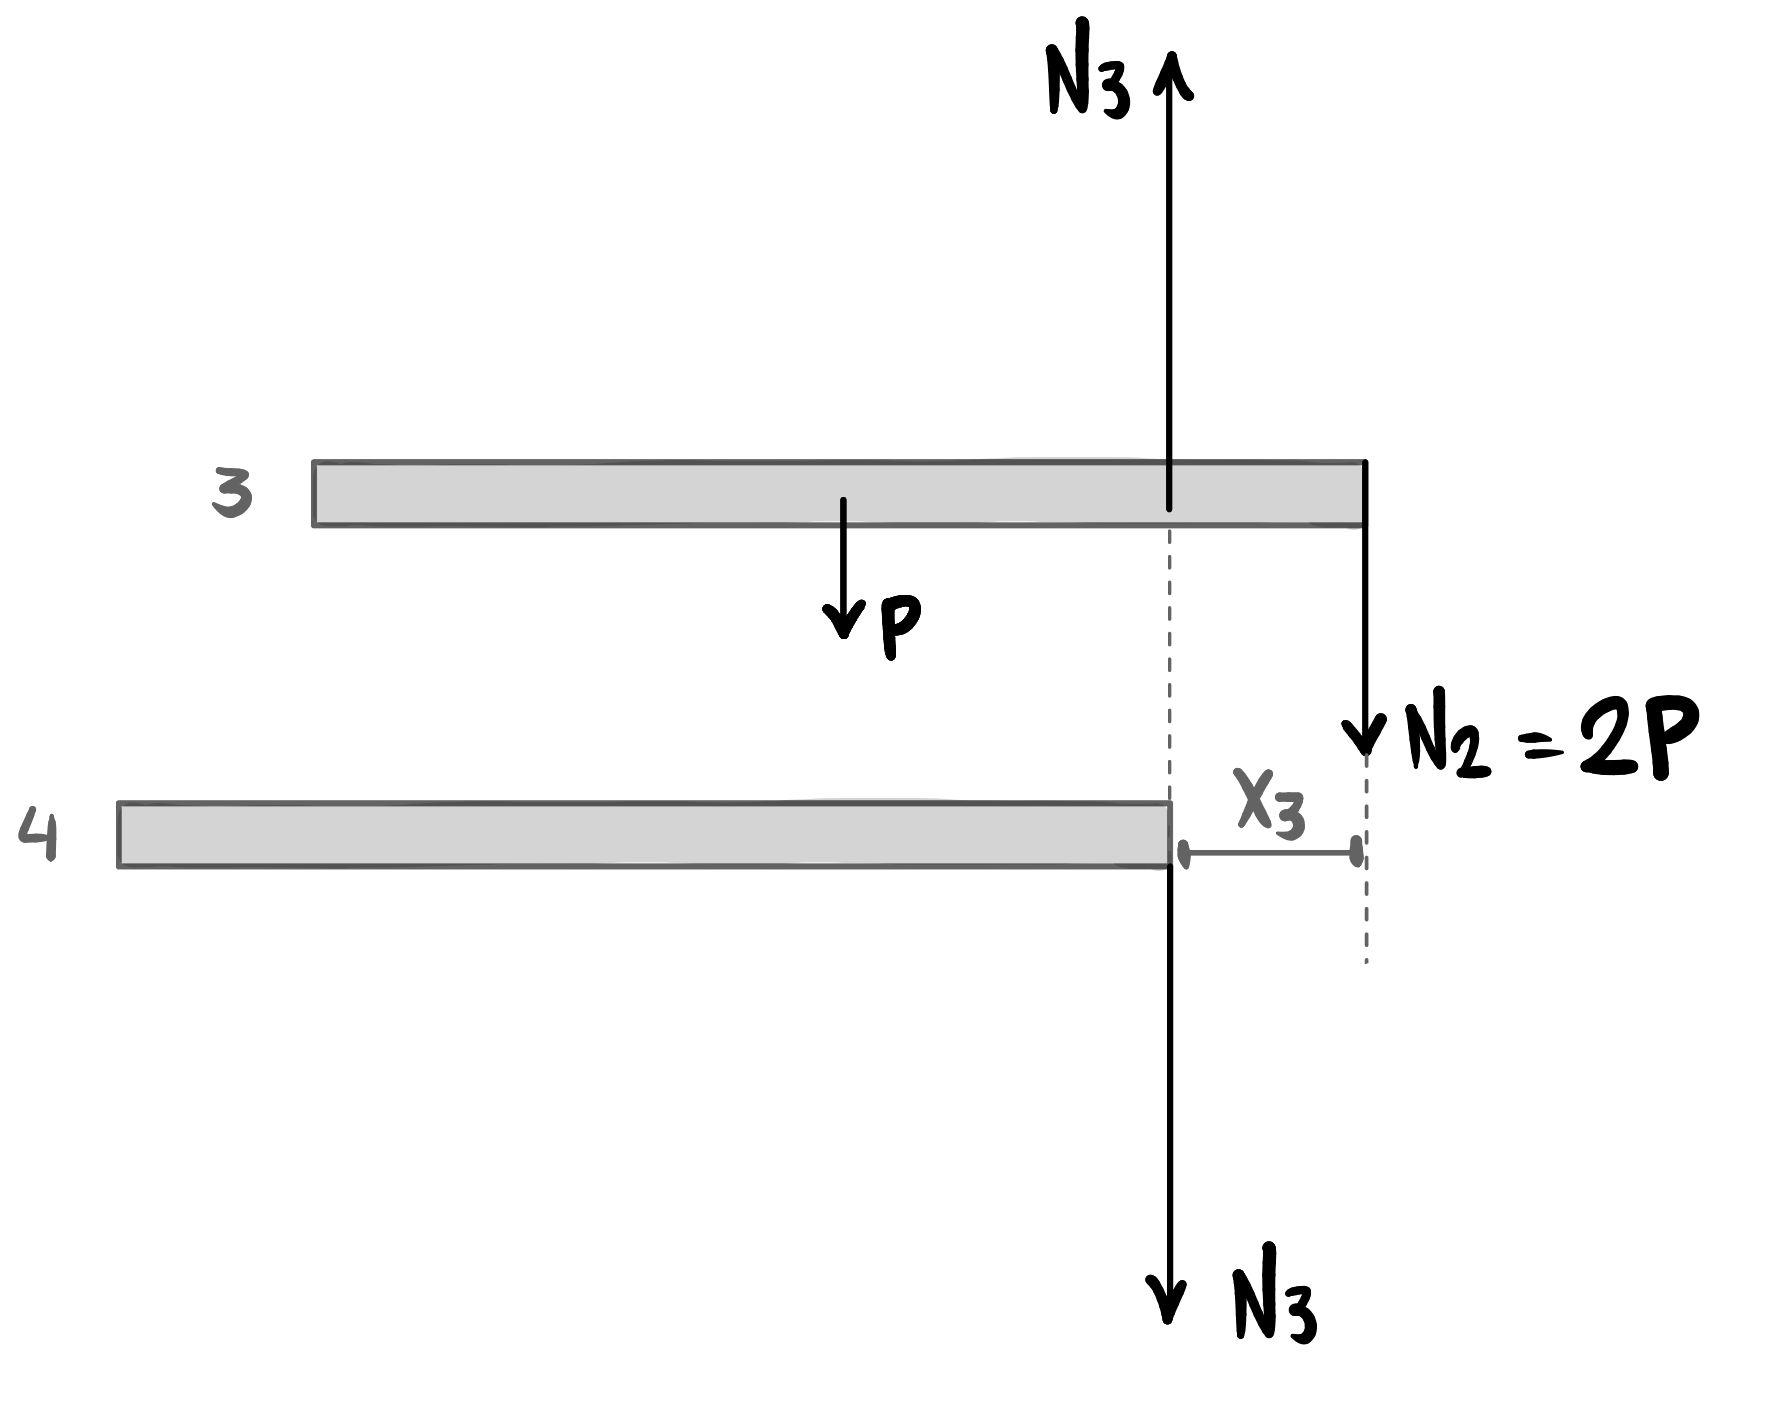
\includegraphics[width=0.45\linewidth]{imagensdinamicarotacao/itaexemplotorquepilhadebarras4.png}};
  \end{scope}
\end{tikzpicture}
\captionof{figure}{Forças nas barras 3 e 4.}
\label{fig_dinamicarotacao_itaexemplotorquepilhadebarras4}
} 
\vspace{0.3cm}

Pelo mesmo argumento, na iminência de tombamento a barra 3 estará com o contato todo concentrando na extremidade da barra 4 -- ponto de aplicação da força normal $N_3.$ Do equilíbrio de torques da barra 3 em relação a tal ponto teremos:

$$ \tau_R = 0 \implies N_2 \cdot x_3 = P \cdot \left( \dfrac{L}{2} - x_3 \right) \implies  2\cancel P \cdot x_3 = \cancel P \cdot \left( \dfrac{L}{2} - x_3 \right) \implies \boxed{x_3= \dfrac{L}{6}.}   $$

Do equilíbrio de forças da barra $3$, temos $N_3 = P + N_2 = 3P.$ Note, portanto, que a força de contato entre as barras -- a normal $N$ -- vai aumentando de $P$ a cada degrau que descemos. Como é ela quem gera o torque no sentido de tombar a barra, é por isso que o avanço $x_k$ de cada barra fica cada vez menor à medida que descemos: o torque $N_{k-1} \cdot x_{k}$ que tende a girar a barra no sentido horário ficaria infinitamente grande caso $x_k$ não diminuísse.

Ora, a essa altura o leitor já deve ter identificado o padrão:

$$x_n = \dfrac{L}{2n},$$

\noindent de modo que a máxima distância $D$ pedida é

$$ D =  x_1 + x_2 + x_3 + \dots + x_n = \dfrac{L}{2} + \dfrac{L}{4} + \dfrac{L}{6} + \dots + \dfrac{L}{2n} = \sum_{k=1}^n \dfrac{L}{2k}. $$

Para o leitor mais analítico, segue a demonstração formal. Generalizando o que fizemos, para a $k-$ésima barra o equilíbrio de torques seria:

$$ N_{k-1} \cdot x_k  = P \left( \dfrac{L}{2} - x_k \right), $$

\noindent em que $N_{k-1} = (k-1)P,$ como o leitor pode verificar para as três primeiras barras. Assim, ter-se-á

$$ (k-1) \cancel P \cdot x_k  = \cancel P \left( \dfrac{L}{2} - x_k \right) \implies \boxed{x_k = \dfrac{L}{2k},} $$

\noindent de modo que a distância $D$ pedida é

$$ \boxed{D =  \sum_{k=1}^n x_k =  \sum_{k=1}^n \dfrac{L}{2k}.} $$

Para $6$ barras teremos

$$ D_6 =  \sum_{k=1}^6 \dfrac{L}{2k} =  \dfrac{L}{2} + \dfrac{L}{4} + \dfrac{L}{6} +  \dfrac{L}{8} + \dfrac{L}{10} + \dfrac{L}{12}  = \dfrac{49L}{40} .$$

\end{exemplo}







% começa com a equação:




\begin{secnivel}[Posição do Centro de Massa]{II}{Posição do Centro de Massa}


\eqLdois{def}{eq_newtonrotacao_posicaocentrodemassa}{x_\text{CM} = \dfrac{m_1 x_1+ m_2 x_2 + \dots m_n x_n }{m_1 + m_2 + \dots + m_n}}

\end{secnivel}



\secgfe{De onde vem}

A Equação \eqref{eq_newtonrotacao_posicaocentrodemassa} determina a posição $x_\text{CM}$ do centro de massa de um sistema de $n$ partículas de massas $m_1, m_2, m_3, \dots, m_n$, localizadas, respectivamente, nas posições $x_1, x_2, x_3, \dots, x_n$ ao longo de um certo eixo $x$ adotado.

Antes de tudo, é preciso compreender o que é exatamente o centro de massa de um corpo extenso (ou de um sistema de partículas). Considere, para tal, a Figura \ref{fig_rotacao_POSICAOCENTROMASSA1}, que mostra duas massas conectadas por uma haste de massa desprezível. Assim, toda a massa do corpo está localizada nos dois extremos. 

\vspace{0.3cm}
{
\centering
\begin{tikzpicture}
  \begin{scope}[blend mode=multiply]
    \node {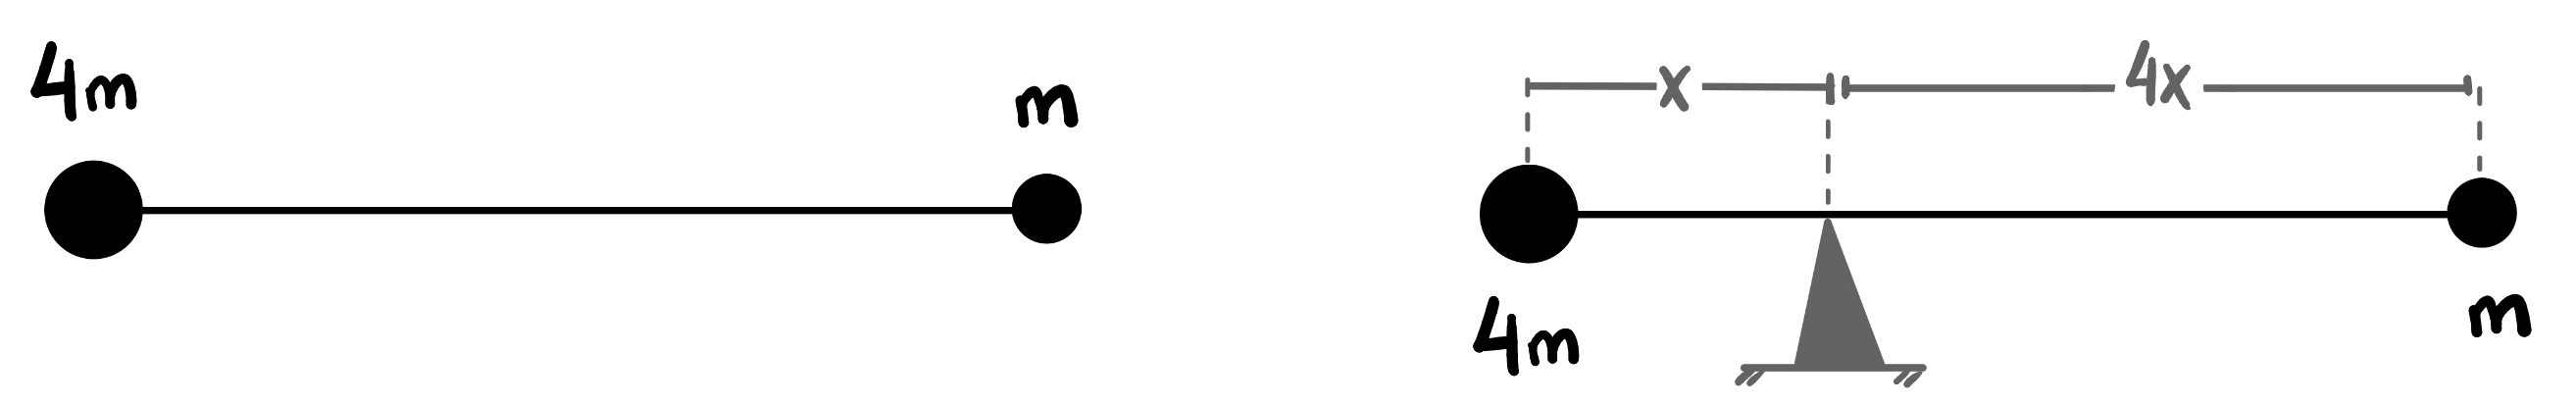
\includegraphics[width=0.8\linewidth]{imagensdinamicarotacao/POSICAOCENTROMASSA1.png}};
  \end{scope}
\end{tikzpicture}
\captionof{figure}{Haltere com duas massas em cada lado, conectadas por uma haste de massa desprezível.}
\label{fig_rotacao_POSICAOCENTROMASSA1}
}
\vspace{0.3cm}

Em qual ponto deveríamos colocar um apoio a fim de manter tal corpo em equilíbrio? Ora, para que o corpo fique em equilíbrio, primeiramente, de rotação, é necessário que o torque resultante seja nulo. Como na direita temos quatro vezes menos massa, o seu peso será quatro vezes menor, de modo que ela precisará de um braço de alavanca quatro vezes maior para gerar o mesmo torque, isto é:

$$ \tau_\text{R} = 0 \implies (4mg) \cdot x = (mg) \cdot 4x,$$

\noindent em que o primeiro membro da equação representa o torque referente ao peso da massa $4m$ em relação ao ponto de apoio e o segundo termo representa o torque referente ao peso da massa $m$ em relação ao mesmo ponto.





Desse modo, conseguimos localizar tal ponto, como mostra a segunda imagem da Figura \ref{fig_rotacao_POSICAOCENTROMASSA1}: ele é tal que sua distância até a massa da esquerda é quatro vezes menor do que sua distância até a massa da direita.

Este ponto é o que se chama de centro de massa da barra: o ponto em relação ao qual o torque total é nulo. Neste caso, poderíamos inclusive imaginar que toda a massa da barra está concentrada neste ponto, como mostra a Figura \ref{fig_rotacao_POSICAOCENTROMASSA2}, e a força peso, portanto, atua apenas ali. Perceba, do lado esquerdo de tal imagem, que aquela é de fato a configuração correta e precisa a respeito das forças que atuam no corpo. Contudo, como ao colocar um apoio sobre o centro de massa o sistema permanece em equilíbrio, caso toda a massa estivesse concentrada ali, a força peso atuaria exclusivamente ali e a dinâmica dos torques seria exatamente a mesma. 

\vspace{0.3cm}
{
\centering
\begin{tikzpicture}
  \begin{scope}[blend mode=multiply]
    \node {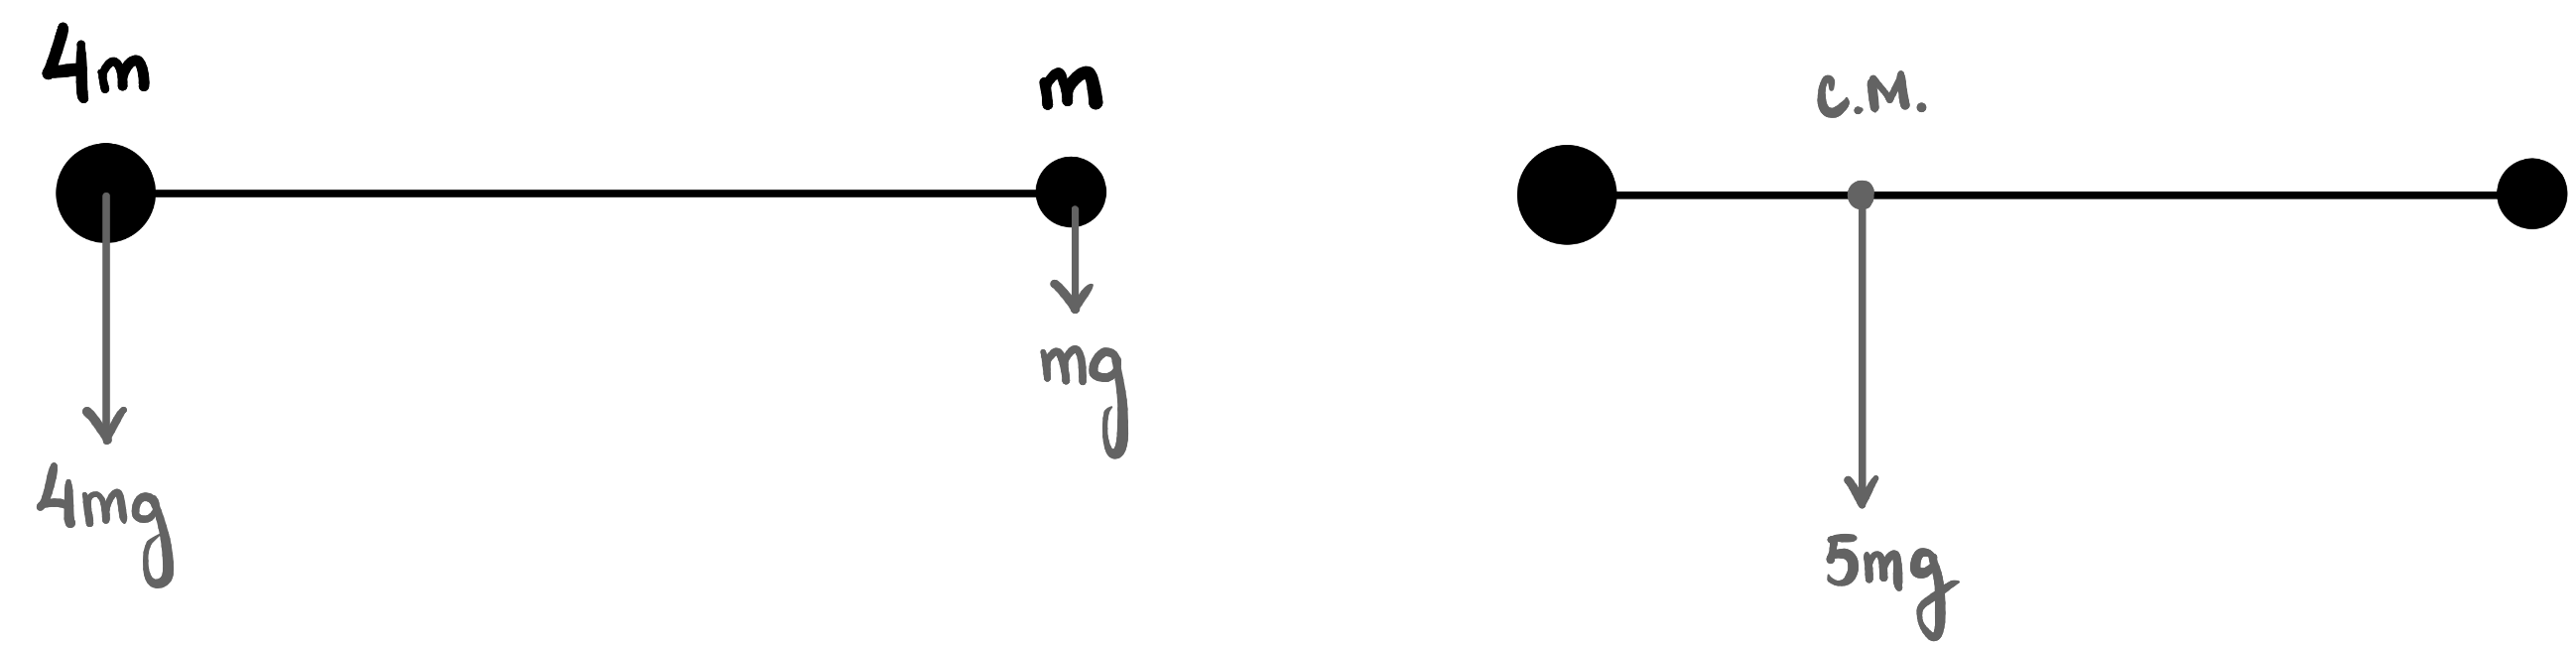
\includegraphics[width=0.8\linewidth]{imagensdinamicarotacao/POSICAOCENTROMASSA2.png}};
  \end{scope}
\end{tikzpicture}
\captionof{figure}{Duas situações que são idênticas do ponto de vista da dinâmica dos torques.}

\label{fig_rotacao_POSICAOCENTROMASSA2}
} 
\vspace{0.3cm}


Assim, o que a Figura \ref{fig_rotacao_POSICAOCENTROMASSA2} se propõe a representar é o seguinte fato: as duas configurações de forças são idênticas do ponto de vista do torque\footnote{Tire a prova: escolha qualquer ponto ao longo da barra e tome os torques em relação a tal ponto para as duas configurações da figura.}, de modo que, considerar que tem-se duas massas nos extremos e levar em conta seus pesos, ou considerar que toda a massa está concentrada no centro de massa e o peso inteiro do objeto atua ali, dá na mesma. 

Desse modo, usando apenas a intuição, é fácil perceber que o centro de massa dessa barra com massas nos extremos ficaria exatamente no seu ponto médio caso as massas fossem iguais: é o ponto no qual poderíamos segurar o sistema sem que ele tombasse (rotacionasse). A Figura \ref{fig_rotacao_cmsimetria} ilustra esse caso e alguns outros em que se destaca a posição do centro de massa: para um disco circular homogêneo (distribuição uniforme de massa) o centro de massa também coincide com seu centro geométrico, uma vez que um diâmetro sempre dividirá o círculo em dois pedaços simétricos, de igual massa.


\vspace{0.3cm}
{
\centering
\begin{tikzpicture}
  \begin{scope}[blend mode=multiply]
    \node {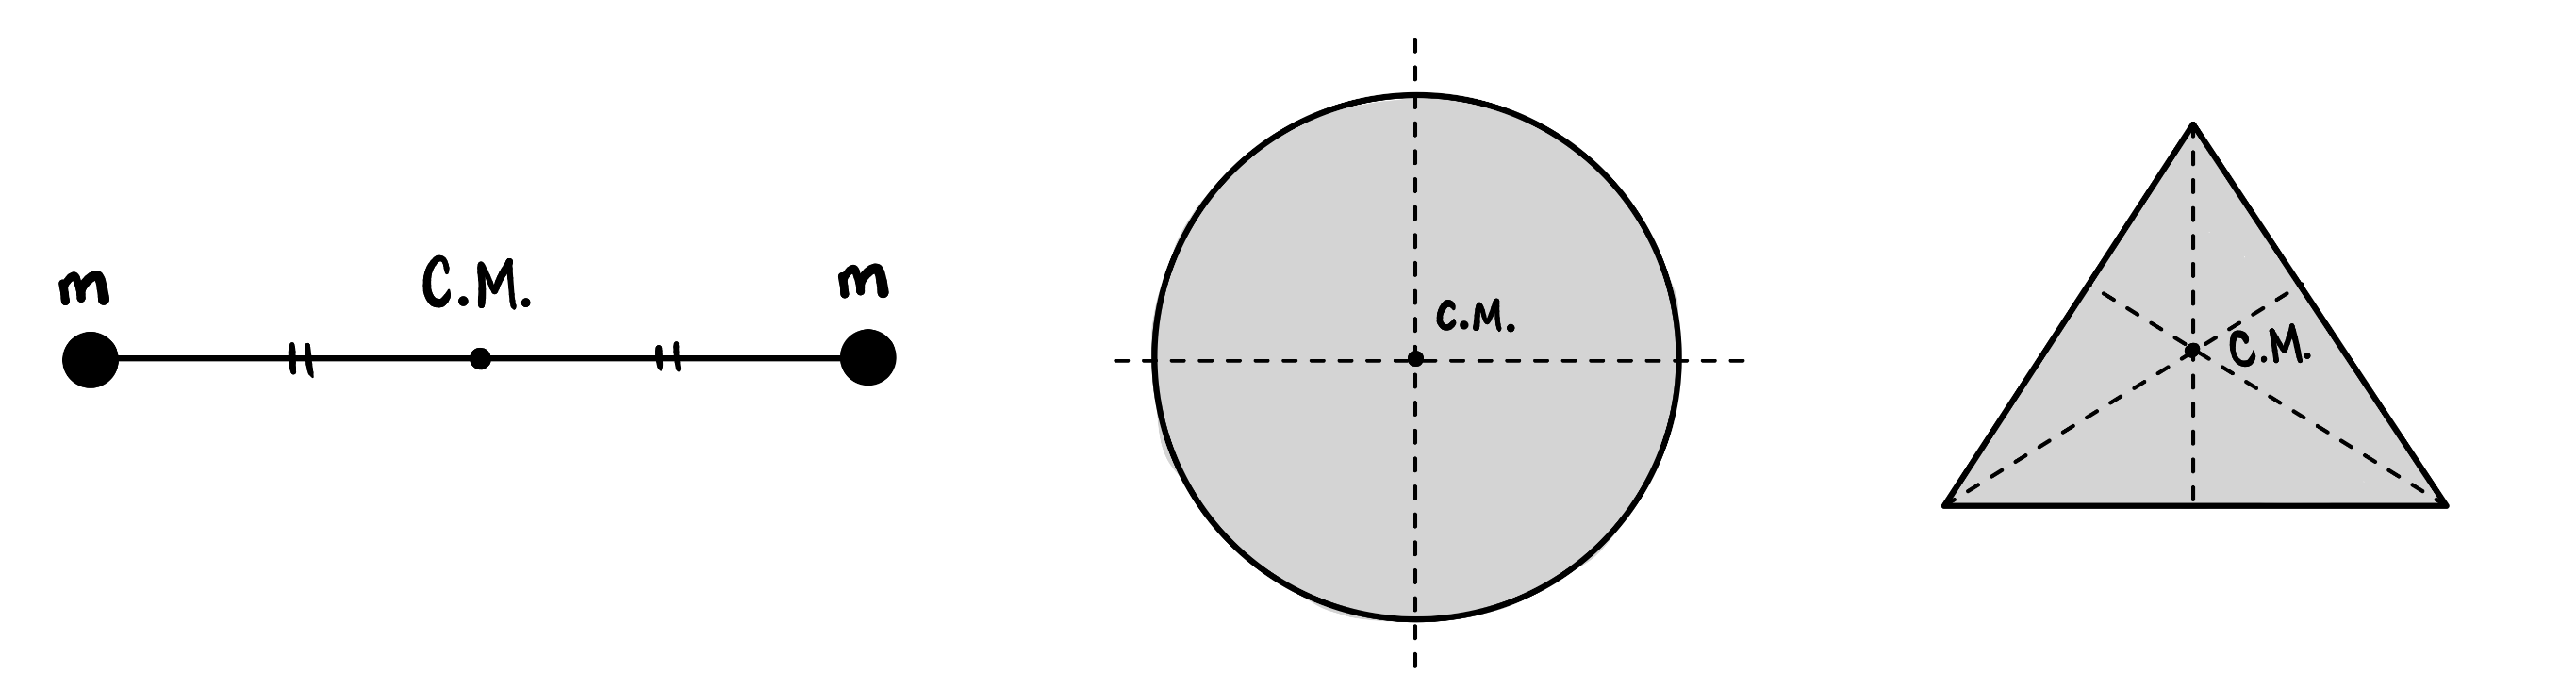
\includegraphics[width=0.9\linewidth]{imagensdinamicarotacao/centrodemassasimetria.png}};
  \end{scope}
\end{tikzpicture}
\captionof{figure}{Posição do centro de massa para alguns objetos específicos.}

\label{fig_rotacao_cmsimetria}
} 
\vspace{0.3cm}

O triângulo, sendo equilátero, terá o seu centro de massa coincidindo com o seu centro geométrico. No caso de um triângulo qualquer, o centro de massa é o baricentro, que é o ponto de encontro das medianas. Tal palavra tem uma etimologia que remonta exatamente ao centro de massa, \textit{báros = }peso e \textit{kéntron} = centro; ou seja, o baricentro é o centro do peso: o ponto em que todo o peso do sistema se concentra.

De modo mais genérico, podemos aplicar toda essa intuição desenvolvida sobre o centro de massa para encontrar uma equação algébrica que nos permita localizá-lo. Isso será feito a partir da Figura \ref{fig_rotacao_POSICAOCENTROMASSA3}, que é análoga àquela da Figura \ref{fig_rotacao_POSICAOCENTROMASSA2}, porém para duas massas genéricas $m_1$ e $m_2.$

\vspace{0.3cm}
{
\centering
\begin{tikzpicture}
  \begin{scope}[blend mode=multiply]
    \node {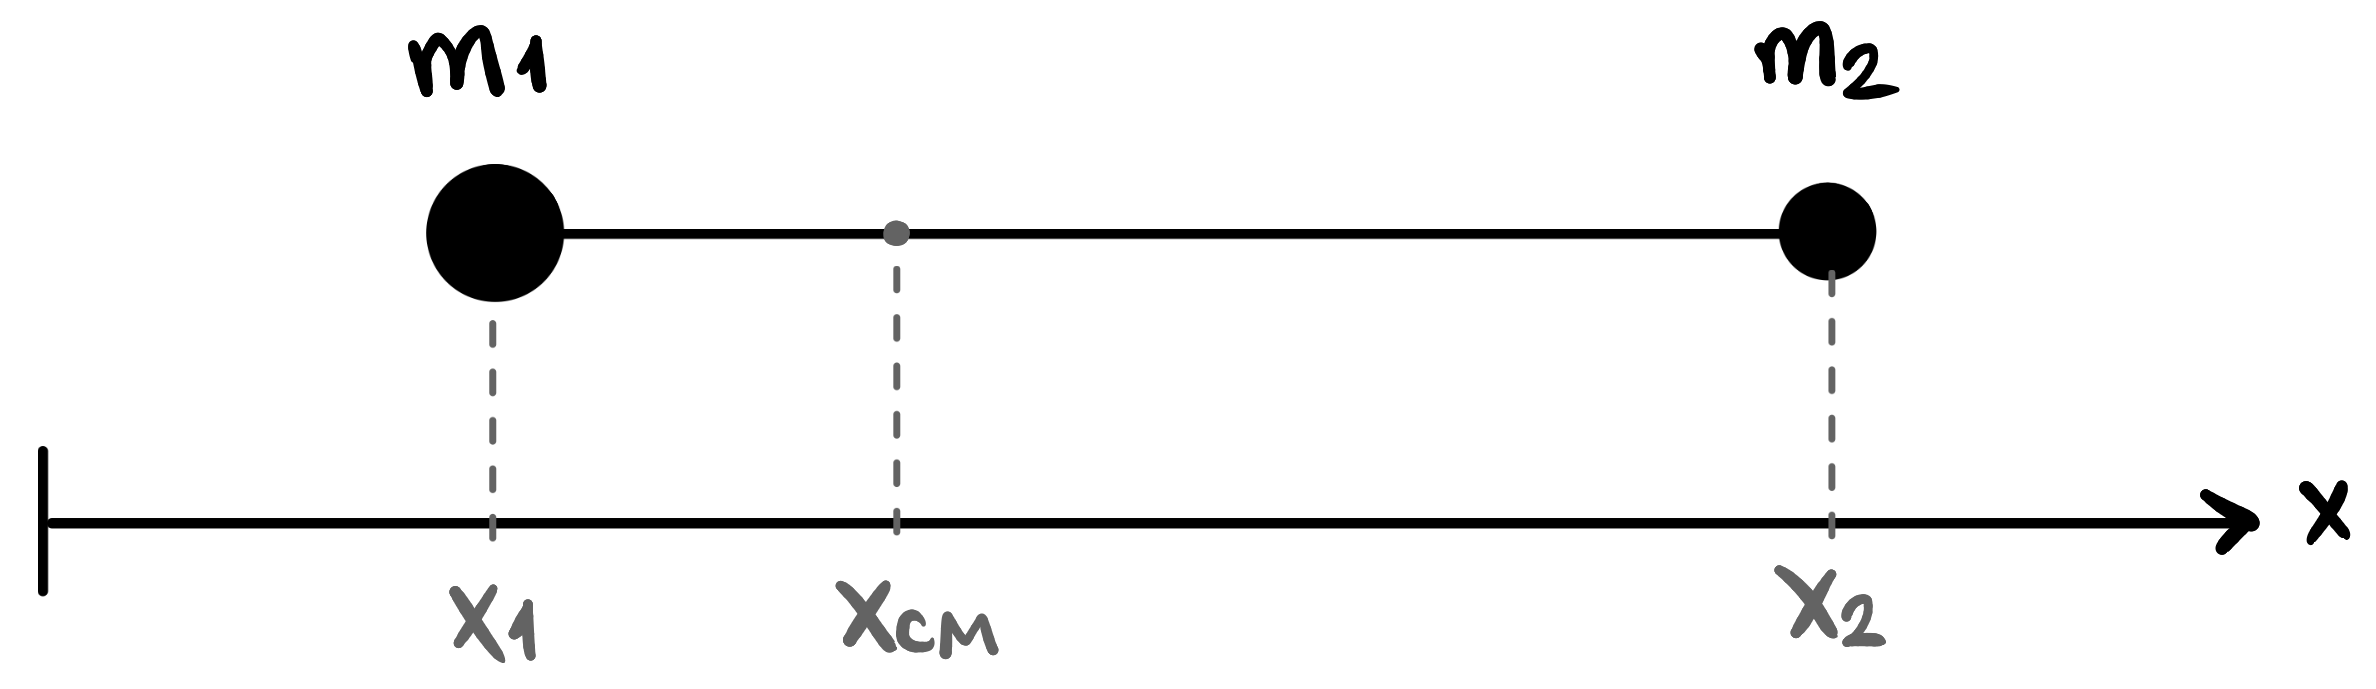
\includegraphics[width=0.45\linewidth]{imagensdinamicarotacao/POSICAOCENTROMASSA3.png}};
  \end{scope}
\end{tikzpicture}
\captionof{figure}{Construindo uma equação que permita localizar o centro de massa.}

\label{fig_rotacao_POSICAOCENTROMASSA3}
} 
\vspace{0.3cm}

Como vimos, a posição $x_\text{CM}$ é aquela que faz com que os torques dos pesos das massas dos extremos se anule, ou seja:

$$ \tau_R = 0 \implies m_1g_1(x_\text{CM}-x_1) = m_2g_2 (x_2 - x_\text{CM} ).$$

Note que pode ocorrer da gravidade ser diferente nos pontos $1$ e $2,$ de tal modo que a relação acima, ao ser desenvolvida, nos forneceria na verdade a posição do \emph{centro de gravidade do corpo}. Contudo, de modo geral, a gravidade é uniforme ao longo da superfície da Terra, de modo que $g_1=g_2=g$ para quase todos os casos. Assim, o centro de gravidade e o centro de massa coincidem:

$$ m_1 \cancel {g_1}(x_\text{CM}-x_1) = m_2 \cancel {g_2}(x_2 - x_\text{CM} ), $$

\noindent o que, desenvolvendo, nos leva a

$$ x_\text{CM} = \dfrac{m_1 x_1 + m_2x_2}{m_1 + m_2}, $$

\noindent que é exatamente o que diz a Equação \eqref{eq_newtonrotacao_posicaocentrodemassa}, porém para um sistema de $n$ massas.

Perceba que o cálculo da posição do centro de massa é uma média ponderada das posições de cada partícula, em que os pesos dessa média são as massas das partículas. Assim, quanto mais massiva for uma partícula, mais ela tende a ``puxar'' o centro de massa para mais próximo de si. 

Nesse sentido, objetos simétricos e homogêneos, como o disco circular da Figura \ref{fig_rotacao_cmsimetria}, possuirão sempre o centro de massa coincidindo com seu centro geométrico: não existe nenhuma parte do corpo com maior concentração de massa. Para qualquer lado que você olhe sempre haverá uma igual quantidade de massa, de modo que o centro de massa deve coincidir com o centro geométrico. Perceba que isso não ocorre na situação da Figura \ref{fig_rotacao_POSICAOCENTROMASSA1}: como há quatro vezes mais massa de um lado do que do outro, o centro de massa fica muito mais próximo desse lado do que do outro -- não coincidindo, portanto, com o centro da barra.




\secgfe{Onde é usada}

A Equação \eqref{eq_newtonrotacao_posicaocentrodemassa} serve para calcular a posição do centro de massa de um sistema discreto de $n$ partículas pontuais, alinhadas ao longo de uma certa dimensão. Podemos, por exemplo, aplicar tal equação para a barra da Figura \ref{fig_rotacao_POSICAOCENTROMASSA1}. Escolhamos, por exemplo, como origem, a posição da massa da esquerda, a qual designaremos por $m_1$, e um eixo $x$ orientado para a direita. Neste caso, sendo $L$ o comprimento da barra, teremos

$$ x_\text{CM} = \dfrac{m_1 \cancelto{0}{x_1} + m_2x_2}{m_1 + m_2}  = \dfrac{mL}{4m + m} = \dfrac{L}{5},$$

\noindent ou seja, se dividirmos a barra em 5 pedaços iguais, de tamanhos $x$, teremos $L=5x$ e o centro de massa estará exatamente a uma distância $\sfrac{L}{5}=x$ da massa da esquerda, exatamente como havíamos previsto de forma intuitiva, e como mostra a Figura \ref{fig_rotacao_POSICAOCENTROMASSA1}.

Perceba que a posição do centro de massa é um ponto específico, porém as suas coordenadas vão depender da escolha do referencial (da origem, no caso). Ou seja, para a mesma situação da Figura \ref{fig_rotacao_POSICAOCENTROMASSA1}, caso adotássemos como referencial um eixo $x$ orientado para a direita, mas com origem na massa da direita, teríamos:

$$ x_\text{CM} = \dfrac{m_1 x_1 + m_2 \cancelto{0}{x_2}}{m_1 + m_2}  = \dfrac{4m(-L)}{4m + m} = -\dfrac{4L}{5},$$

\noindent ou seja, se dividirmos a barra em 5 pedaços iguais, de tamanhos $x$, teremos $L=5x$, e o centro de massa estará exatamente a uma distância $\sfrac{4L}{5}=4x$, para a esquerda, da massa da direita. Perceba que isso representa exatamente a mesma posição calculada anteriormente, apenas usando um sistema de referência diferente. Desse modo, o centro de massa é um ponto físico do espaço que não muda, porém suas coordenadas dependem da escolha da origem e da orientação do eixo $x.$


\secgfe{Erros comuns}

A Equação \eqref{eq_newtonrotacao_posicaocentrodemassa} serve para um sistema de partículas alinhadas ao longo da mesma direção, exatamente como nos casos vistos, de uma barra horizontal com massas amarradas em seus extremos. Para um objeto (ou um sistema de partículas) bidimensional, teríamos que usar duas vezes tal equação, para computar a coordenada horizontal $x_\text{CM}$ do centro de massa e sua coordenada vertical $y_\text{CM}$, dada exatamente pela mesma expressão, porém agora considerando as posições verticais $y_i$ das partículas:

$$ \boxed{y_\text{CM} = \dfrac{m_1 y_1+ m_2 y_2 + \dots m_n y_n }{m_1 + m_2 + \dots + m_n} .} $$

Assim, para corpos bidimensionais, é necessário separar as direções vertical e horizontal e aplicar duas vezes a equação para localizar as coordenadas $y$ e $x$ do centro de massa. Considere, por exemplo, um objeto em forma de $L$, composto por duas barras rígidas de tamanho $2a,$ conectadas em um ângulo reto. Se as duas barras são homogêneas, sendo $m$ suas massas, os seus centros de massa coincidem com o seu centro geométrico.

\vspace{0.3cm}
{
\centering
\begin{tikzpicture}
  \begin{scope}[blend mode=multiply]
    \node {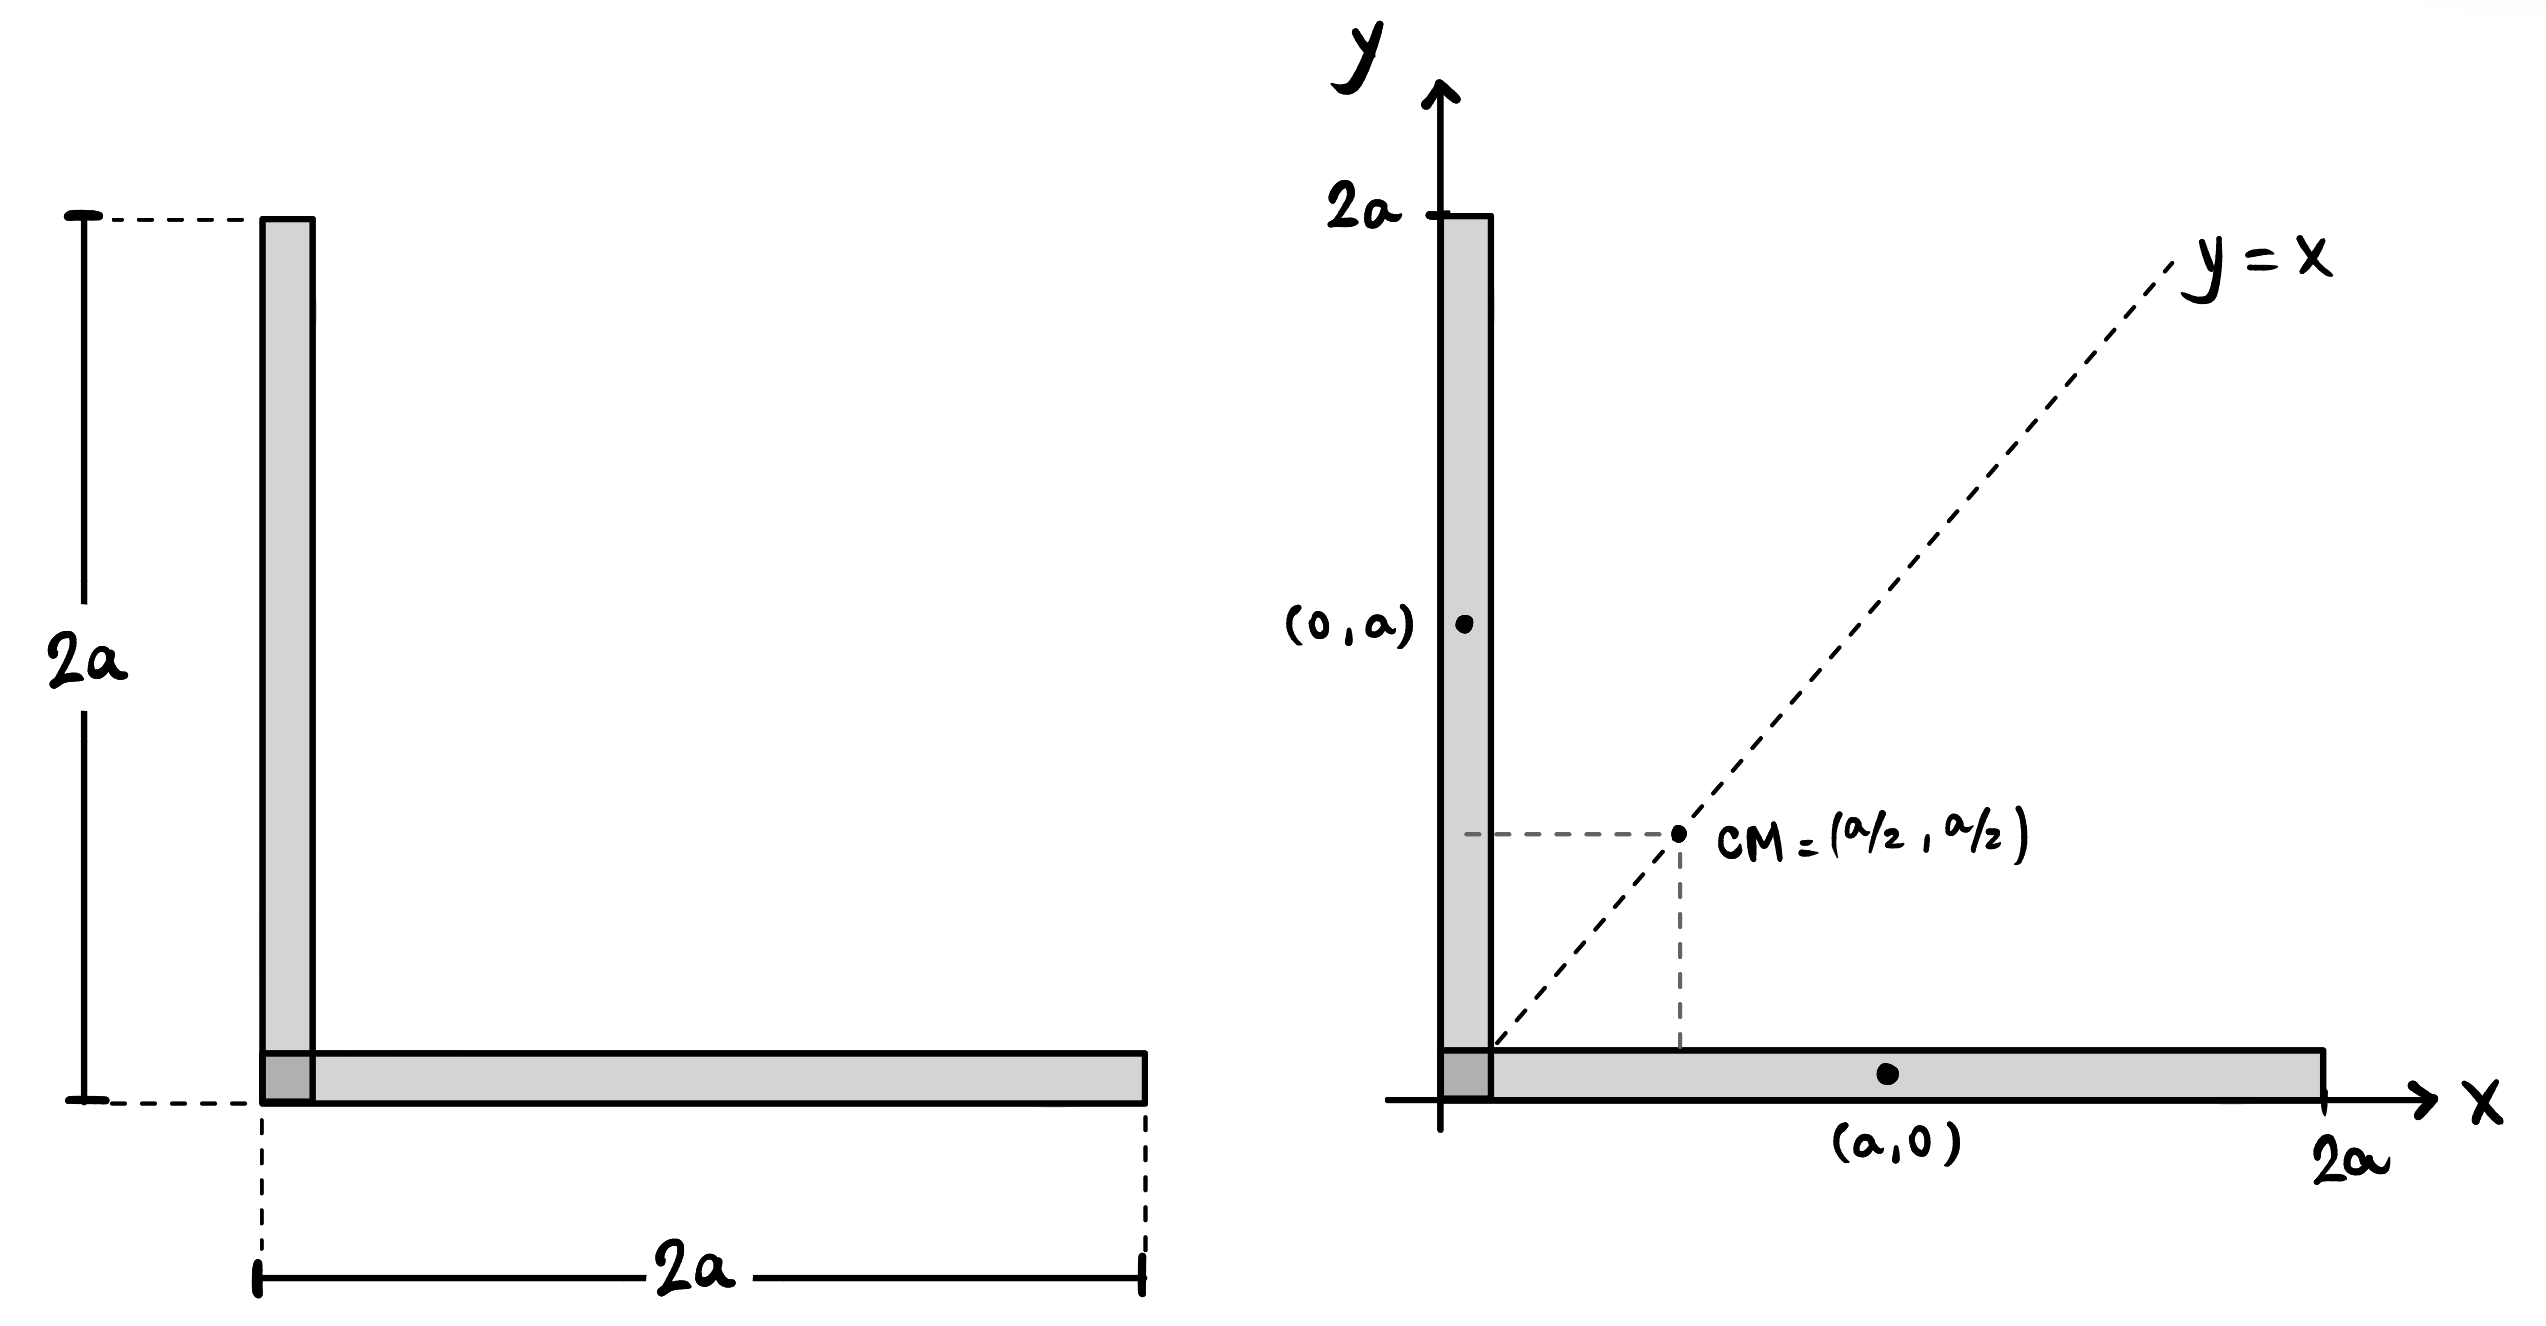
\includegraphics[width=0.75\linewidth]{imagensdinamicarotacao/centrodemassa2dbarral.png}};
  \end{scope}
\end{tikzpicture}
\captionof{figure}{Centro de massa do frame em $L$ composto por duas barras homogêneas de tamanho $2a$.}

\label{fig_rotacao_barraemlcm}
} 
\vspace{0.3cm}


Assim, a barra $1$, horizontal, possui as coordenadas do seu centro de massa dadas por $(x_1 , y_1) = (a,0)$; enquanto a barra $2,$ vertical, possui seu centro de massa na posição $(x_2 , y_2) = (0,a).$ Desse modo, o centro de massa da barra em $L$ (sistema compostos pelas barras $1$ e $2$) tem posições dadas por

\begin{align}
    x_\text{CM} & = \dfrac{m_1 x_1 + m_2x_2}{m_1 + m_2} = \dfrac{m \cdot a + m \cdot 0}{m+m} = \dfrac{a}{2} \nonumber \\
     y_\text{CM} & = \dfrac{m_1 y_1 + m_2y_2}{m_1 + m_2} =  \dfrac{m \cdot 0 + m \cdot a}{m+m} = \dfrac{a}{2}, \nonumber
\end{align}

\noindent ou seja, a posição do centro de massa é dada pelas coordenadas $(x_\text{CM} \text{ , } y_\text{CM}) = (\sfrac{a}{2} \text{ , } \sfrac{a}{2}  )$, como mostra a segunda imagem da Figura \ref{fig_rotacao_barraemlcm}. Duas coisas são importantes de se notar neste resultado:

\begin{enumerate}
    \item O centro de massa é um ponto que não pertence ao objeto. 

    Como mostra a segunda imagem da Figura \ref{fig_rotacao_barraemlcm}, o centro de massa da barra em $L$ é um ponto que está fora da barra. Isso pode parecer estranho em um primeiro momento, mas é razoável: o centro de massa é computado por meio de uma média ponderada das posições das partículas, e médias ponderadas não precisam coincidir com nenhum dos valores que as compõem. A média de dois números pode estar entre eles sem ser nenhum deles. 

    O centro de massa, portanto, é um ponto matemático, abstrato: não precisa ser um ponto material do objeto. O fato do C.M. ser um ponto externo ao corpo significa, fisicamente, que não existe nenhum ponto material pertencente à barra tal que, ao colocar um apoio na barra sob aquele ponto, ela fique em equilíbrio. Seriam necessários dois ou mais pontos de apoio para manter tal objeto em equilíbrio.


   \item O centro de massa, neste caso, pertence à bissetriz dos quadrantes pares -- a reta $y=x$.

   Isso ocorre pelo fato de o corpo ser simétrico em relação a tal reta. Se você dobrar a figura sobre essa reta, os dois braços se sobrepõem exatamente. O CM de qualquer figura\footnote{Qualquer figura homogênea, isto é, com distribuição uniforme de massa.} com um eixo de simetria $\ell$ precisa estar sobre esse eixo.
   
   Existe uma forma de ver isso que dispensa contas completamente, apoiada em dois fatos: (i)~o CM é único -- para um dado sistema de massas, existe exatamente um CM, sem ambiguidade;\footnote{Para o leitor mais analítico, isso por ser compreendido pelo fato de que a Equação \eqref{eq_newtonrotacao_posicaocentrodemassa} é linear em $x$, fornecendo, portanto, um único valor possível para $x_\text{CM}.$} (ii)~a figura é invariante pela reflexão em torno do eixo $\ell$ -- a distribuição de massa é idêntica antes e depois dessa operação. Suponha, por absurdo, que o CM esteja num ponto $G$ fora de $\ell$. Ao refletir toda a figura, a distribuição de massa não muda, logo o CM da figura refletida deve continuar sendo $G$. Mas geometricamente a reflexão leva $G$ a um ponto $G' \neq G$, simétrico de $G$ em relação a $\ell$ — de modo que a figura refletida teria CM em $G'$. Note que temos uma contradição: a mesma figura não pode ter dois CMs distintos. A única saída é $G = G'$, o que ocorre se e somente se $G$ estiver sobre $\ell$.


    
\end{enumerate}

\secgfe{Observações}

Cabem aqui duas observações relevantes, que faremos no seu devido lugar.

\subsubsection{Velocidade do Centro de Massa}

Na Equação \eqref{eq_newtonrotacao_posicaocentrodemassa}, o denominador é simplesmente a massa total $M_\text{T}$ do sistema, de modo que tal equação pode ser escrita como

$$ x_\text{CM} = \dfrac{m_1x_1 + m_2x_2 + \dots + m_nx_n}{M_\text{T}}.$$

Se quisermos falar de variações de posições ao invés de apenas posições específicas, poderíamos reescrever a equação acima na forma 

$$ \Delta x_\text{CM} = \dfrac{m_1 \Delta x_1 + m_2 \Delta x_2 + \dots + m_n \Delta x_n}{M_\text{T}},$$

\noindent e, dividindo os dois lados da equação acima por $\Delta t$ -- que seria o intervalo de tempo necessário para que ocorrer os deslocamentos $\Delta x$ -- teremos

$$ \dfrac{\Delta x_\text{CM}}{\Delta t} = \dfrac{m_1 \dfrac{\Delta x_1}{\Delta t} + m_2 \dfrac{\Delta x_2}{\Delta t} + \dots + m_n \dfrac{\Delta x_n}{\Delta t}}{M_\text{T}},$$

\noindent ou seja:

$$  v_\text{CM} = \dfrac{m_1 v_1 + m_2 v_2 + \dots + m_n v_n}{M_\text{T}},$$

\noindent em que $v_1, v_2, \dots v_n$ são as velocidades de cada uma das partículas, e $v_\text{CM}$ é a velocidade do centro de massa do sistema. A expressão acima ainda pode ser reescrita como 

$$  M_\text{T} \cdot v_\text{CM} =  m_1 v_1 + m_2 v_2 + \dots + m_n v_n. $$ 

Contudo, perceba que o lado direito é simplesmente o momento linear total do sistema, isto é, $p_\text{sistema} = m_1v_1 + m_2v_2 + \dots m_nv_n.$ Logo, veja que, considerando toda a massa do sistema concentrada no seu centro de massa, podemos computar o momento linear total do sistema simplesmente fazendo $p=mv$, usando a massa total do sistema e a velocidade do centro de massa:


$$ p_\text{sistema}=  M_\text{T} \cdot v_\text{CM}. $$

Porém, como já vimos no estudo da Equação \eqref{eq_newton_convervacaomomentolinear}, o momento linear de um sistema não se altera sob a ação de forças internas. Desse modo, podemos dizer, pela equação acima, que a velocidade do centro de massa de um sistema não se altera pela ação de forças internas.


\vspace{0.3cm}
{
\centering
\begin{tikzpicture}
  \begin{scope}[blend mode=multiply]
    \node {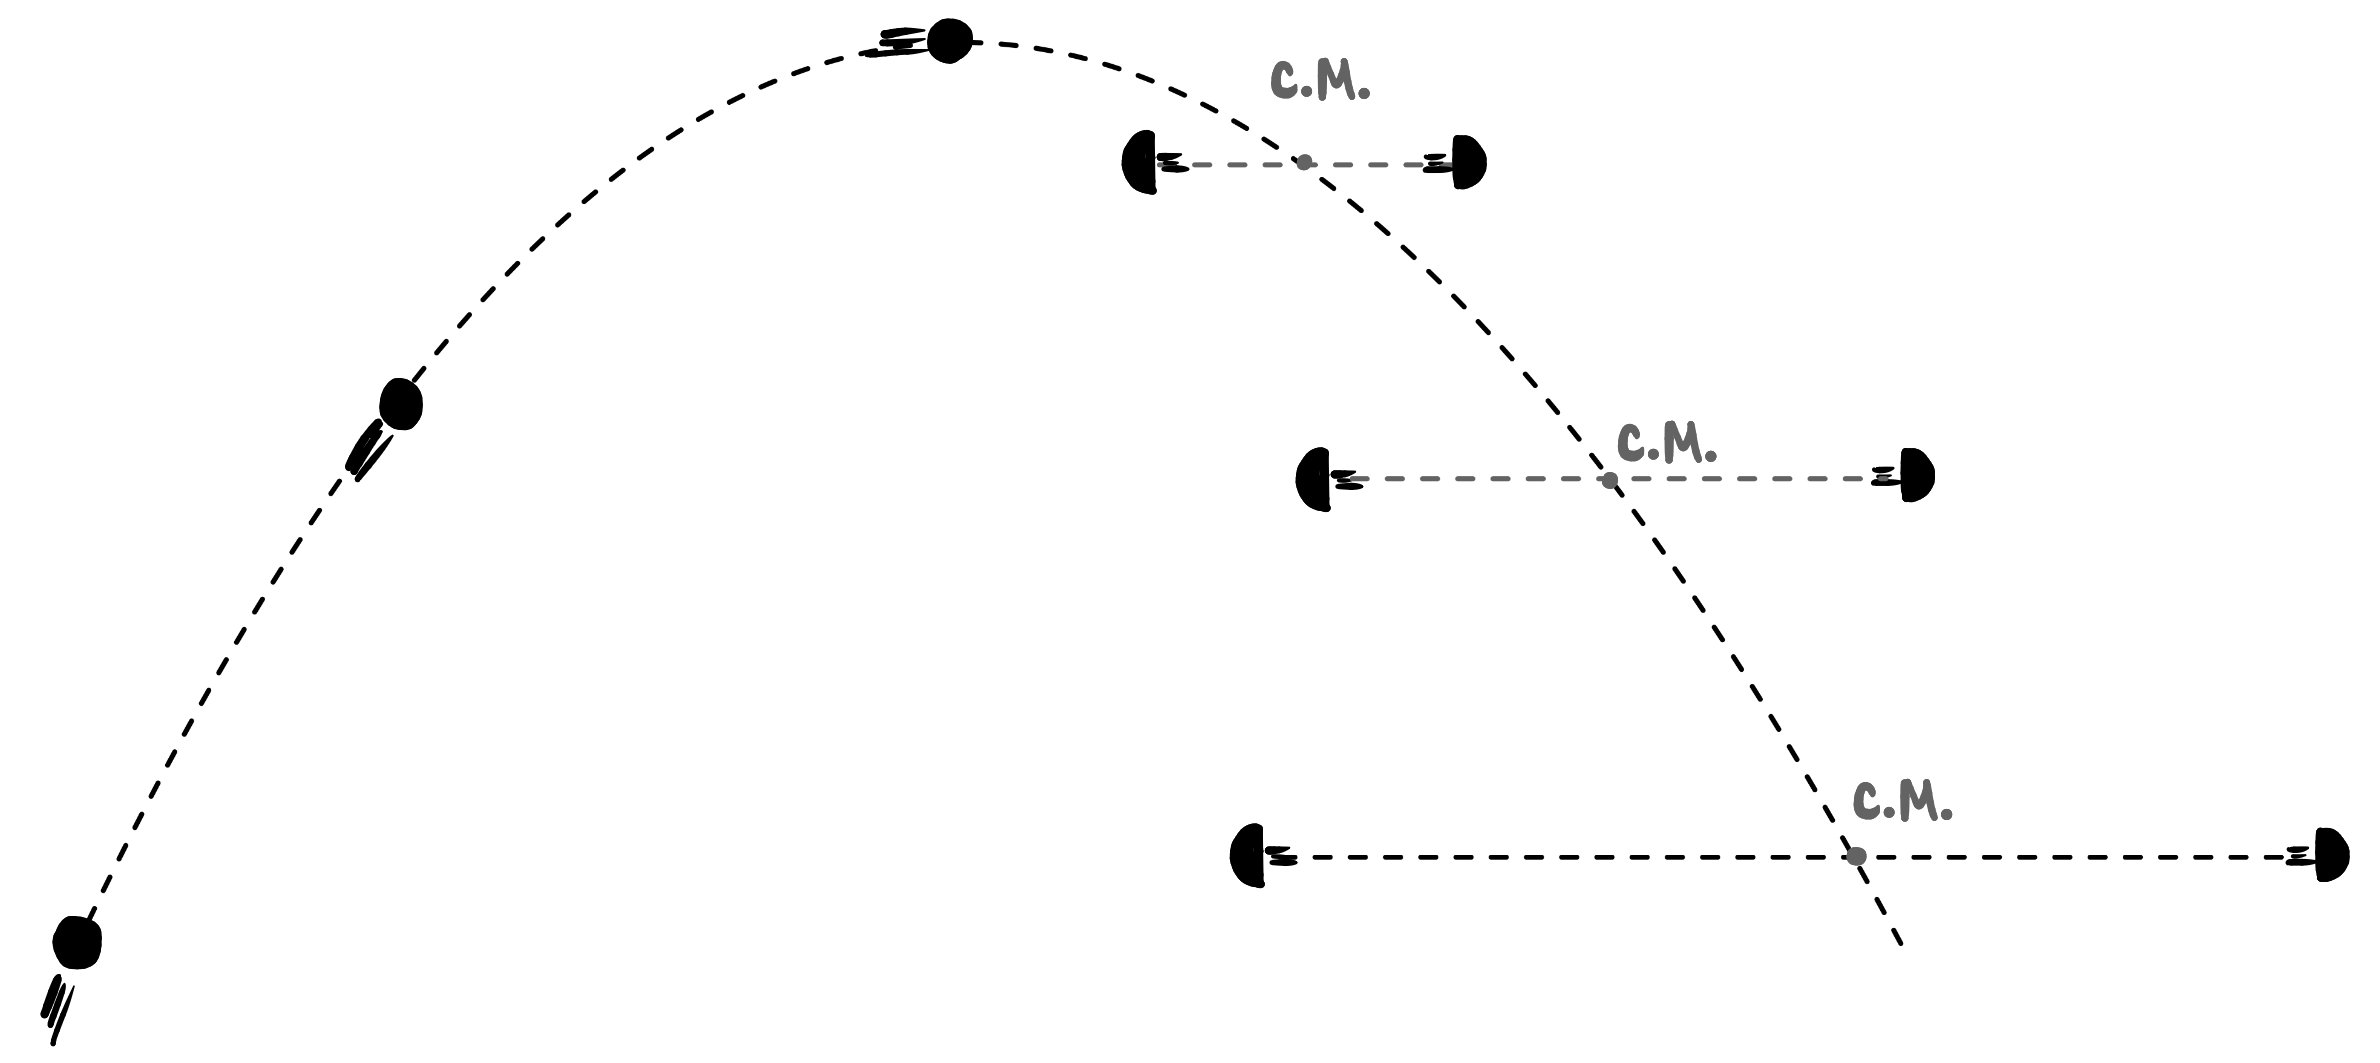
\includegraphics[width=0.50\linewidth]{imagensdinamicarotacao/POSICAOCENTROMASSA4.png}};
  \end{scope}
\end{tikzpicture}
\captionof{figure}{A velocidade do centro de massa não muda sob a ação de forças internas.}

\label{fig_rotacao_POSICAOCENTROMASSA4}
} 
\vspace{0.3cm}

Assim, como mostra a Figura \ref{fig_rotacao_POSICAOCENTROMASSA4}, se um certo corpo segue uma trajetória parabólica e, no ponto de altura máxima, ele explode, se fragmentando em dois pedaços, tais pedaços vão se mover de tal modo que o centro de massa continue descrevendo exatamente a mesma parábola: forças internas (da explosão) não alteram a velocidade do centro de massa de um sistema.


\subsubsection{Estabilidade e Centro de Massa}

Observe a Figura \ref{fig_rotacao_estabilidadecentrodemassa1}, que mostra uma barra homogênea em cima de uma mesa. Ao deslocar a barra para a direita, a partir de quando a barra irá tombar? Ora, como mostra a figura, tão logo o seu centro de massa passar da extremidade da mesa ela irá tombar: nessa situação a força peso passa a gerar um torque no sentido horário em relação à extremidade da mesa.

\vspace{0.3cm}
{
\centering
\begin{tikzpicture}
  \begin{scope}[blend mode=multiply]
    \node {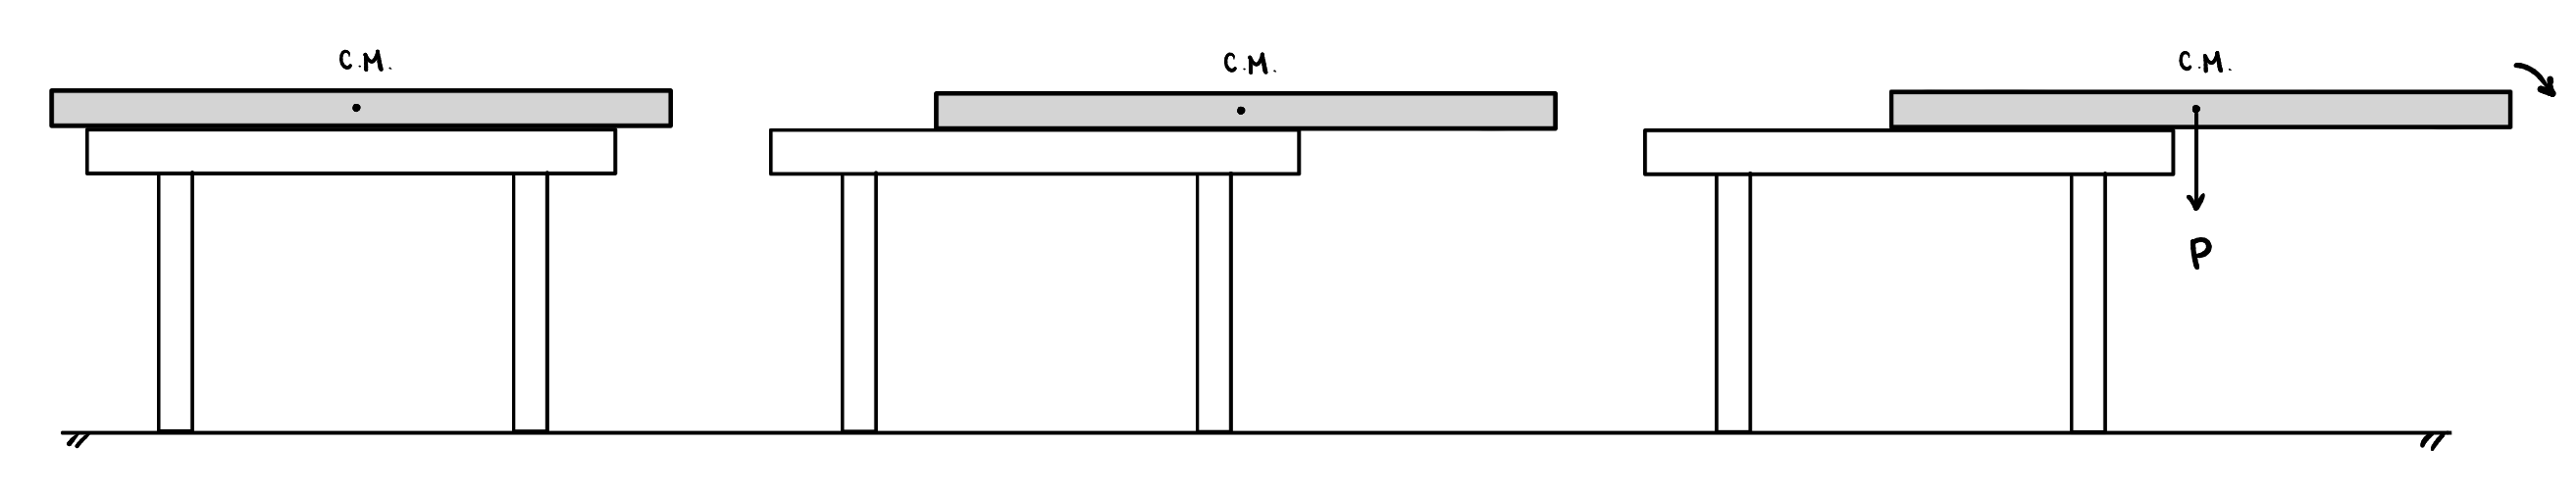
\includegraphics[width=0.9\linewidth]{imagensdinamicarotacao/estabilidadecentrodemassa1.png}};
  \end{scope}
\end{tikzpicture}
\captionof{figure}{A barra tomba para fora da mesa tão logo a linha vertical que passa pelo seu centro de massa passar pela extremidade da mesa.}

\label{fig_rotacao_estabilidadecentrodemassa1}
} 
\vspace{0.3cm}


Isso introduz uma interessante discussão: qual é a relação entre a posição do centro de massa e a estabilidade de uma posição de equilíbrio? Observe a Figura \ref{fig_rotacao_estabilidadecentrodemassa2}, que mostra uma caixa homogênea, inicialmente em equilíbrio. Vamos girá-la, a partir do ponto $O,$ no sentido anti-horário. Como o leitor pode ver, para as duas primeiras posições de giro, o equilíbrio é \emph{estável:} a linha vertical que passa pelo centro de massa está à direita do ponto $O,$, de modo que o torque do peso tende a girar a caixa no sentido horário, trazendo-a de volta à sua posição de equilíbrio.


\vspace{0.3cm}
{
\centering
\begin{tikzpicture}
  \begin{scope}[blend mode=multiply]
    \node {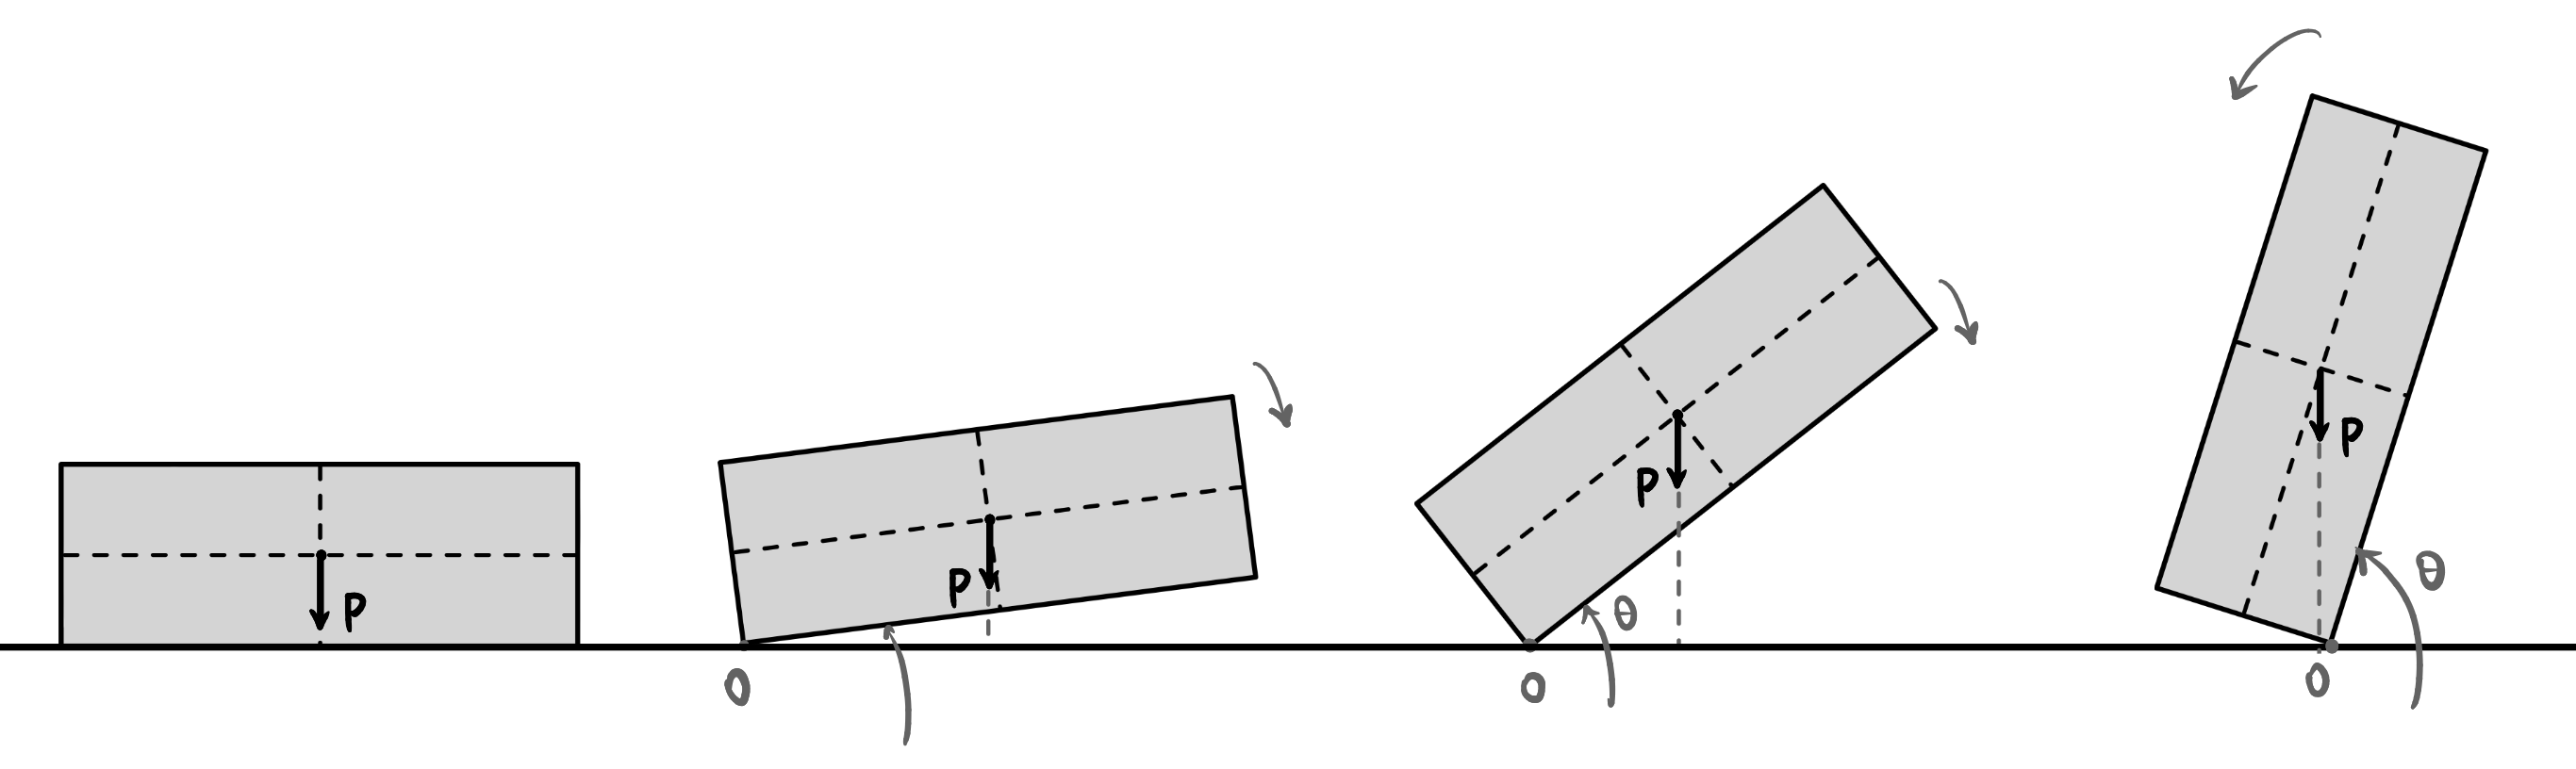
\includegraphics[width=0.95\linewidth]{imagensdinamicarotacao/estabilidadecentrodemassa2.png}};
  \end{scope}
\end{tikzpicture}
\captionof{figure}{Quanto mais baixo for o centro de massa mais estável é o equilíbrio.}

\label{fig_rotacao_estabilidadecentrodemassa2}
} 
\vspace{0.3cm}


Já na última situação da Figura \ref{fig_rotacao_estabilidadecentrodemassa2} nós tombamos tanto a caixa que agora a linha vertical que passa pelo centro de massa está à esquerda do ponto $O,$ de modo que o torque do peso tende a girar a caixa no sentido anti-horário, fazendo a caixa tombar, agora, neste sentido.

A Figura \ref{fig_rotacao_estabilidadecentrodemassa3} mostra melhor esse contraste. Temos agora uma caixa não homogênea, com o centro de massa bem alto. A imagem do meio mostra uma pequena rotação feita em relação ao ponto $O,$ no sentido anti-horário, na caixa. Nessa posição, a linha vertical que passa pelo centro de massa está à direita do ponto $O,$ de modo que o torque do peso tende a girar a caixa no sentido horário, trazendo-a de volta à sua posição de equilíbrio.




\vspace{0.3cm}
{
\centering
\begin{tikzpicture}
  \begin{scope}[blend mode=multiply]
    \node {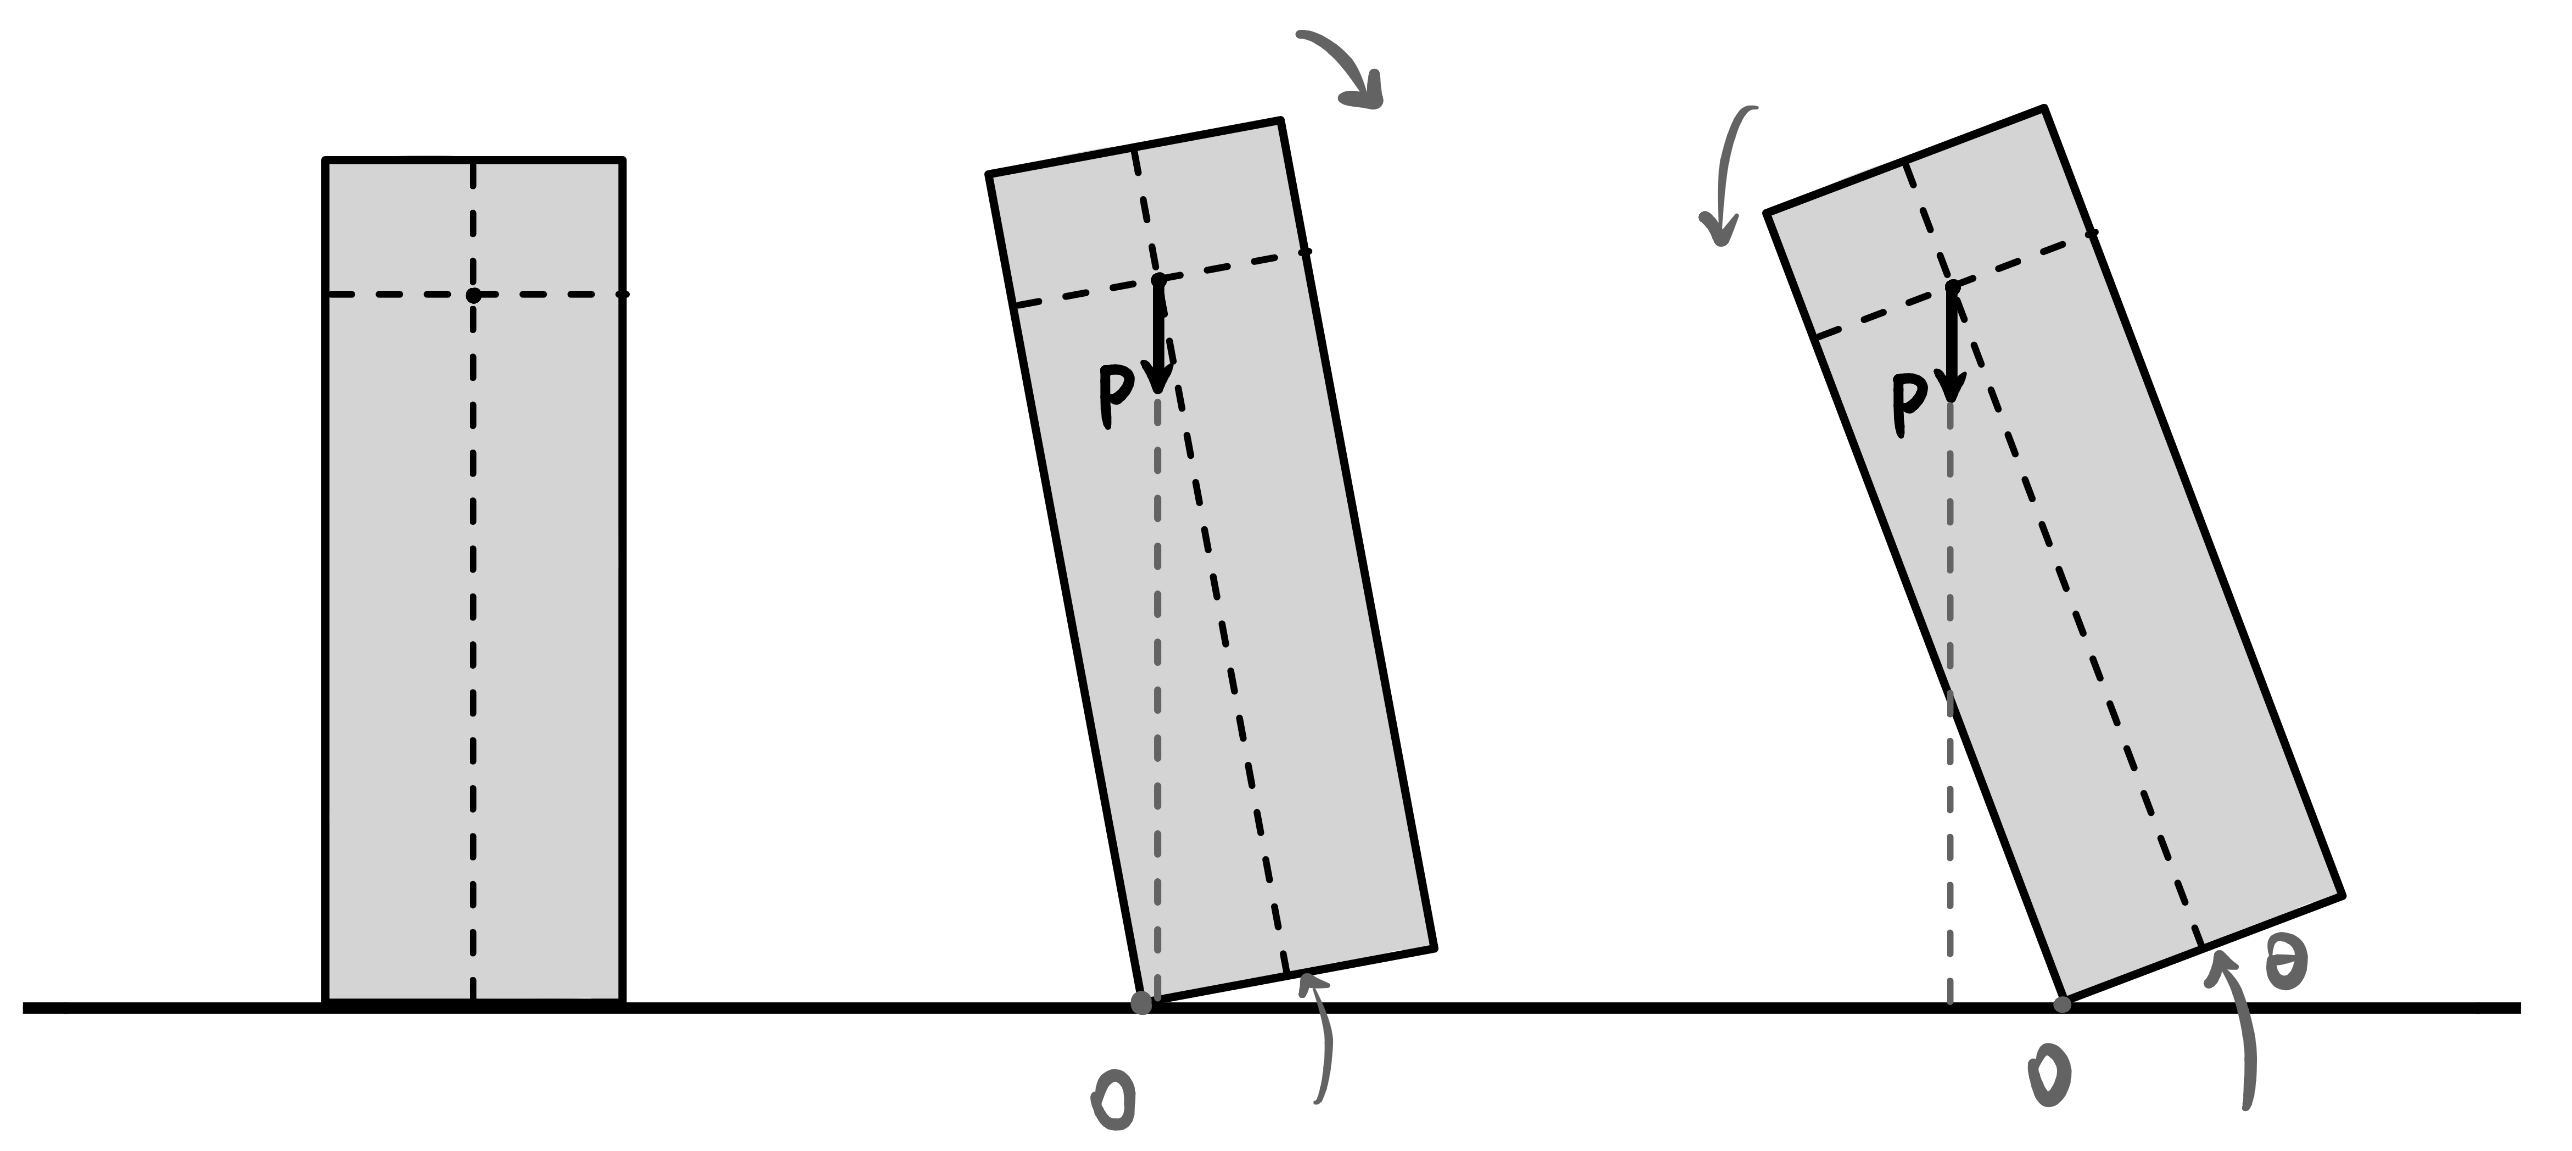
\includegraphics[width=0.7\linewidth]{imagensdinamicarotacao/estabilidadecentrodemassa3.png}};
  \end{scope}
\end{tikzpicture}
\captionof{figure}{Quanto mais alto for o centro de massa mais instável é o equilíbrio.}

\label{fig_rotacao_estabilidadecentrodemassa3}
} 
\vspace{0.3cm}

Contudo, ao girar a caixa nesse sentido só um pouco a mais, como mostra a última imagem da figura, o seu centro de massa já troca de posição em relação ao ponto $O:$ agora a linha vertical que passa pelo centro de massa está à esquerda do ponto $O,$ de modo que o torque do peso tende a girar a caixa no sentido anti-horário, fazendo a caixa tombar, agora, neste sentido.

Dizemos que corpos com centro de massa mais altos possuem equilíbrio mais \emph{instáveis}: pequenas perturbações fazem com que o torque do peso tenda a tombá-los. Já corpos com centro de massa mais baixos, como o da Figura \ref{fig_rotacao_estabilidadecentrodemassa2}, são mais \emph{estáveis:} sob perturbações o torque do peso tende a trazê-los de volta para a posição de equilíbrio. 




\vspace{0.3cm}

\begin{exemplo}[Nível II]\label{exemplo_dinamicarotacao_centrodemassaex01}

Mostre que o centro de massa de um triângulo qualquer está no ponto de encontro das suas medianas -- o seu baricentro $G$.

\resolucao

Vamos começar modelando o triângulo homogêneo como uma coleção de faixas muito finas, paralelas ao lado $BC$. O centro de massa de cada faixa (um segmento homogêneo) está no seu ponto médio. O lugar geométrico dos pontos médios de todas essas faixas é exatamente a mediana $\overline{AP}$, onde $P$ é o ponto médio de $\overline{BC}$. Pela propriedade do CM, o centro de massa do triângulo deve, portanto, estar sobre a mediana $\overline{AP}$.


\vspace{0.3cm}
{
\centering
\begin{tikzpicture}
  \begin{scope}[blend mode=multiply]
    \node {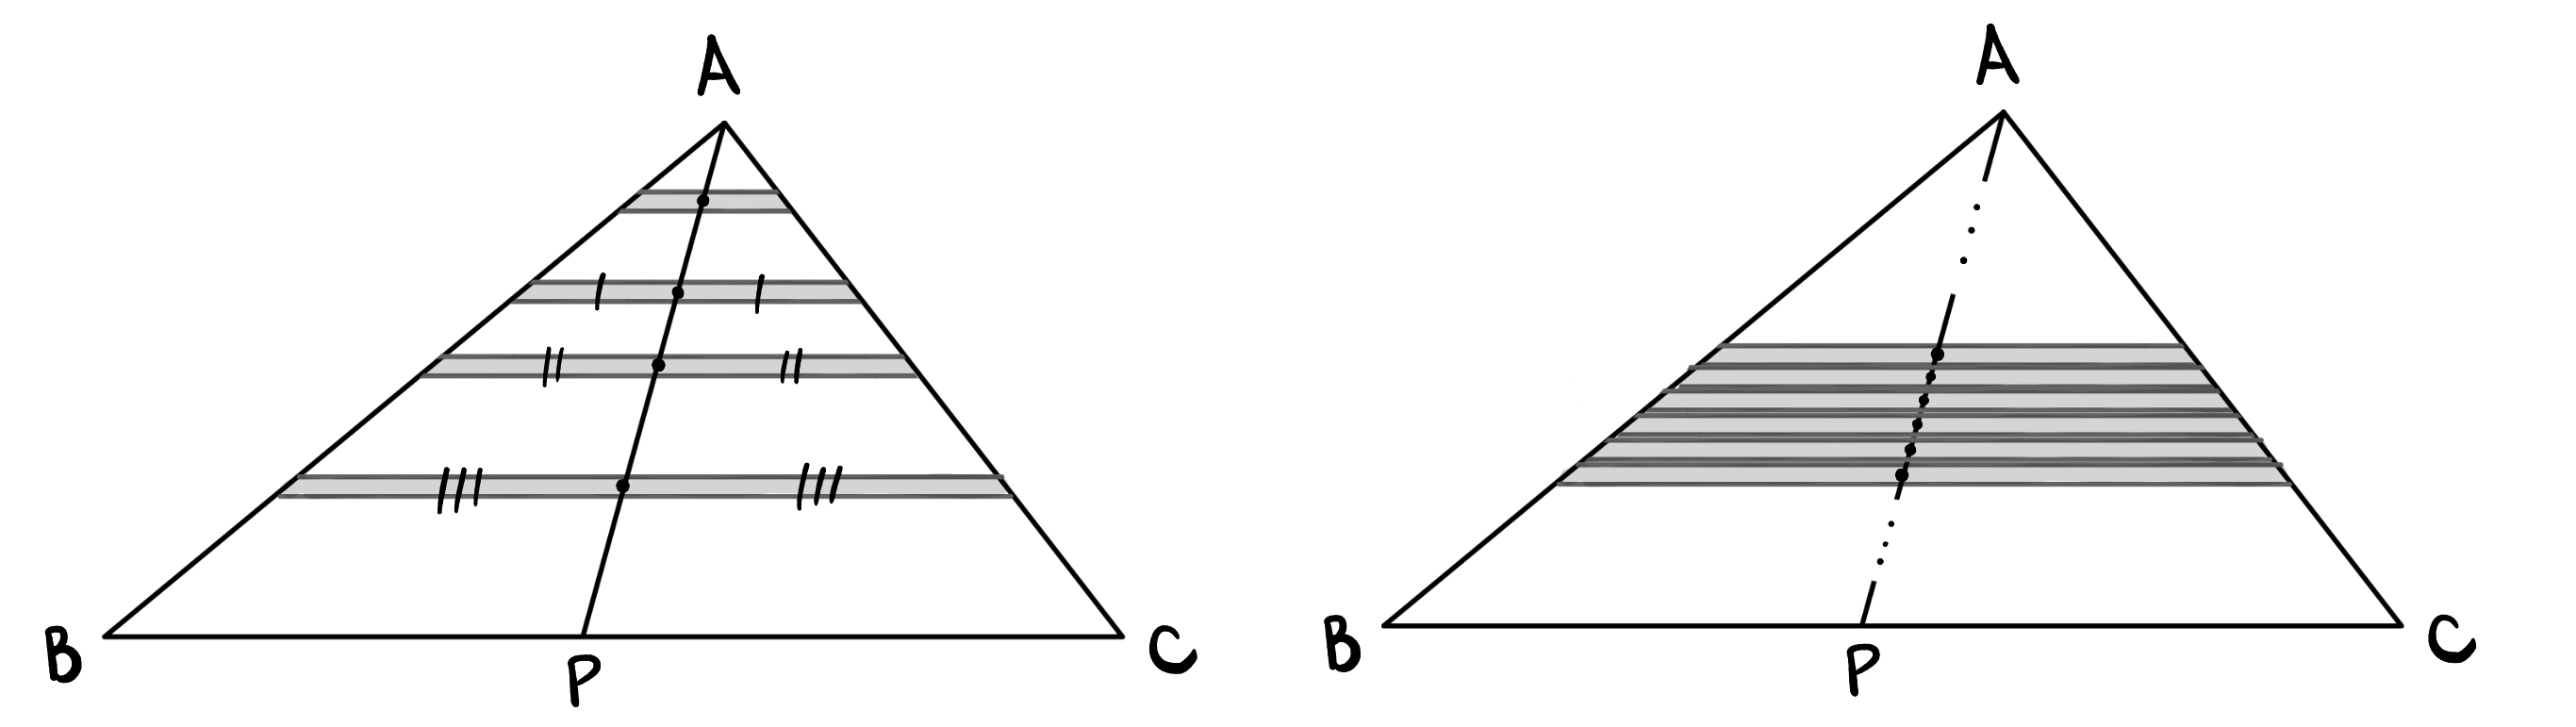
\includegraphics[width=0.85\linewidth]{imagensdinamicarotacao/centromassatriangulo.png}};
  \end{scope}
\end{tikzpicture}
\captionof{figure}{O centro de massa de um triângulo qualquer.}

\label{fig_rotacao_centromassatriangulo}
} 
\vspace{0.3cm}



O mesmo argumento, aplicado a faixas paralelas a $\overline{AC}$ e a $\overline{AB}$, mostra que o CM deve estar igualmente sobre as medianas $\overline{BQ}$ e $\overline{CS}$, em que $Q$ e $S$ são os pontos médios de $\overline{AC}$ e $\overline{AB},$ respectivamente. Como as três medianas de um triângulo concorrem num único ponto (seu baricentro $G$), e o CM deve pertencer simultaneamente às três, conclui-se que o centro de massa coincide com o ponto de encontro das medianas -- o baricentro. 

\end{exemplo}







\vspace{0.3cm}



\begin{exemplo}[Nível III (ITA 2015)]\label{exemplo_dinamicarotacao_centrodemassaex02}

Uma chapa metálica homogênea quadrada de $100\ \text{cm}^2$ de área, situada no plano $xy$ de um sistema de referência, com um dos lados no eixo $x$, tem o vértice inferior esquerdo na origem. Dela, retira-se uma porção circular de $5{,}00\ \text{cm}$ de diâmetro com o centro posicionado em $x = 2{,}50\ \text{cm}$ e $y = 5{,}00\ \text{cm}$.

Determine as coordenadas do centro de massa da chapa restante.

\begin{enumerate}
    \item[(a)] $(x_C, y_C) = (6{,}51,\ 5{,}00)\ \text{cm}$
    \item[(b)] $(x_C, y_C) = (5{,}61,\ 5{,}00)\ \text{cm}$
    \item[(c)] $(x_C, y_C) = (5{,}00,\ 5{,}61)\ \text{cm}$
    \item[(d)] $(x_C, y_C) = (5{,}00,\ 6{,}51)\ \text{cm}$
    \item[(e)] $(x_C, y_C) = (5{,}00,\ 5{,}00)\ \text{cm}$
\end{enumerate}

\resolucao

A Figura \ref{fig_rotacao_centrodemassaitaexemplo3} ilustra a situação. Seja $A$ o disco circular, $B$ a chapa com o furo e $C$ a chapa plana completa. Queremos encontrar o centro de massa do objeto $B$, ou seja, queremos as coordenadas $(x_B\text{ , }y_B)$ do seu centro de massa.

Observando a imagem do meio da Figura \ref{fig_rotacao_centrodemassaitaexemplo3}, vemos que a chapa com o furo se trata de uma figura simétrica em relação à reta $y=5$ cm. Assim, é evidente que a posição vertical do centro de massa deve estar sob tal reta, ou seja, $y_B = 5$ cm. 


\vspace{0.3cm}
{
\centering
\begin{tikzpicture}
  \begin{scope}[blend mode=multiply]
    \node {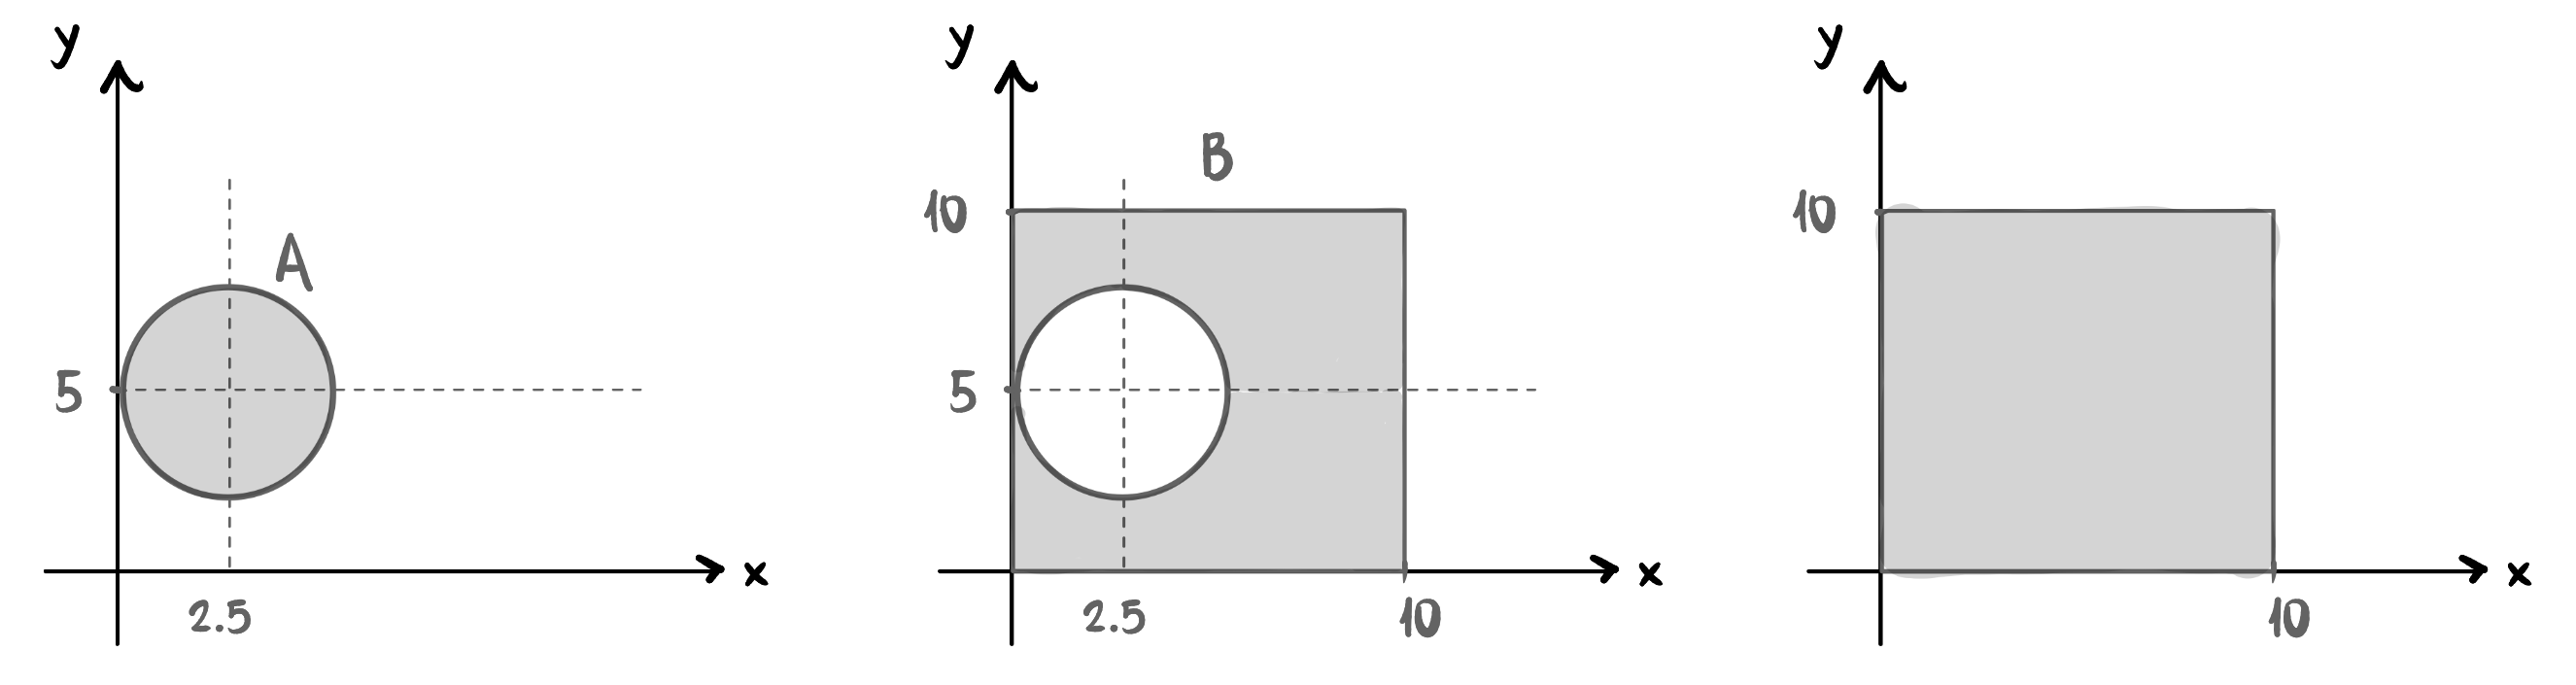
\includegraphics[width=0.9\linewidth]{imagensdinamicarotacao/centrodemassaitaexemplo3.png}};
  \end{scope}
\end{tikzpicture}
\captionof{figure}{}

\label{fig_rotacao_centrodemassaitaexemplo3}
} 
\vspace{0.3cm}

Para obter a coordenada horizontal do centro de massa, observe que o corpo $C$ é formado pelos corpos $A$ e $B$ sobrepostos, ou seja, podemos escrever, pela Equação \eqref{eq_newtonrotacao_posicaocentrodemassa}, que

$$ x_\text{C} = \dfrac{m_\text{A} x_\text{A} + m_\text{B} x_\text{B} }{m_\text{A} + m_\text{B}}.$$

Para o corpo $A$ temos $x_A = 2.5$ cm, e sua massa será proporcional à sua área, ou seja, $m_A = \sigma \pi 2.5^2.$ Para o corpo $B$ teremos $m_B = \sigma (10^2 - \pi 2.5^2)$; e para o corpo $C$ temos $x_c = 5$. Assim, na equação acima, teremos


$$ 5 = \dfrac{\cancel\sigma \pi 2.5^2 \cdot 2.5 + \cancel \sigma (10^2 - \pi 2.5^2) x_\text{B} }{\cancel \sigma 10^2},$$

\noindent o que, desenvolvendo, nos leva a $x_B \approx 5.61 $. Desse modo, as coordenadas do centro de massa do objeto $B$ (placa furada) são

$$ \boxed{ (x_B\text{ , }y_B) = (5.61 \text{ , } 5.00) \implies \text{ letra B. }}$$




\end{exemplo}

\vspace{0.3cm}


\begin{exemplo}[Nível III]\label{exemplo_dinamicarotacao_centrodemassaex03}

Ao longo de uma reta são distribuídos, em intervalos iguais a $d$, pontos materiais de massas
$m$, $m/2$, $m/4$, $m/8$, \ldots\,. Determinar o centro de massa do sistema.

\begin{enumerate}
    \item[a)] A posição do centro de massa coincide com a de $m$
    \item[b)] A posição do centro de massa coincide com a de $m/2$
    \item[c)] A posição do centro de massa coincide com a de $m/4$
    \item[d)] O centro de massa equidista de $m/2$ e $m/4$
    \item[e)] O centro de massa equidista de $m$ e $m/2$
\end{enumerate}


\resolucao

Considere um eixo horizontal $x$, tal que sua origem coincida com a posição da primeira partícula, de massa $m$. A posição do centro de massa é dada, pela Equação \eqref{eq_newtonrotacao_posicaocentrodemassa}, por


$$ x_\text{CM} = \dfrac{m \cancelto{0}{x_1}+ (\sfrac{m}{2}) \cdot d + (\sfrac{m}{4}) \cdot 2d +  (\sfrac{m}{8}) \cdot 3d + \dots  }{m + \sfrac{m}{2} + \sfrac{m}{4} + \sfrac{m}{8} + \dots }$$

\noindent o que pode ser simplificado para

$$ x_\text{CM} = \left( \dfrac{\sfrac{1}{2} + \sfrac{2}{4} + \sfrac{3}{8} + \sfrac{4}{16} + \dots }{1 + \sfrac{1}{2} +  \sfrac{1}{4} +  \sfrac{1}{8} + \dots }  \right) \cdot d .$$

O denominador é a soma dos infinitos termos da progressão geométrica de razão $q = \sfrac{1}{2}$ e termo inicial $a_1=1,$ cuja soma é conhecida, e vale

$$ S_{\infty} = \dfrac{a_1}{1-q} = \dfrac{1}{1-\sfrac{1}{2}} = 2.$$

O numerador consiste na soma 

\begin{equation}
    \sum_{n=1}^{\infty} \dfrac{n}{2^n},
    \label{eq_centrodemassa_exemplo}
\end{equation}


\noindent que será simplificada como se segue. Considere, de modo genérico, a soma de $nx^n,$ isto é:

$$ S =  \sum_{n=1}^{\infty} nx^n  = 0 + x + 2x^2 + 3x^3+4x^4 + \dots$$

Multiplicando os dois lados por $x$, teremos

$$ xS = x^2 + 2x^3 + 3x^4 + 4x^5 + \dots$$

\noindent e, subtraindo $xS$ de $S$, ficamos com

$$   S - xS = x + x^2 + x^3+ x^4 +  \dots $$

Note que o lado direito é uma progressão geométrica infinita, de razão $q=x$ e termo inicial $a_1=x$. Se $q=x$ for tal que $0<x<1,$ então a soma dos infinitos termos converge, sendo dada por

$$ S'= \dfrac{a_1}{1-q} = \dfrac{x}{1-x}.$$

Logo, teremos 

$$ S-xS = S(1-x) = \dfrac{x}{1-x} \implies \boxed{S =  \sum_{n=1}^{\infty} nx^n =\dfrac{x}{(1-x)^2} \text{ para } 0<x<1.}$$

Perceba que o nosso denominador, dado pela soma expressa na Equação \eqref{eq_centrodemassa_exemplo}, é exatamente desse tipo, com $x=\sfrac{1}{2},$ ou seja, teremos  

$$  \sum_{n=1}^{\infty} \dfrac{n}{2^n} = \dfrac{\sfrac{1}{2}}{(1-\sfrac{1}{2})^2} = 2.$$

Assim, a posição do centro de massa é

$$ x_\text{CM} = \left( \dfrac{\sfrac{1}{2} + \sfrac{2}{4} + \sfrac{3}{8} + \sfrac{4}{16} + \dots }{1 + \sfrac{1}{2} +  \sfrac{1}{4} +  \sfrac{1}{8} + \dots }  \right) \cdot d  = \dfrac{2}{2} \cdot d = d,$$

\noindent ou seja, o centro de massa coincide com a posição da segunda partícula, de massa $m/2$, o que nos dá como resposta a letra B.

\end{exemplo}



\vspace{0.3cm}


















\begin{secnivel}[Teorema das 3 Forças]{III}{Teorema das 3 Forças}
 

  \eqLdois{dem}{eq_newtonrotacao_terorema3forcas}{\vec F_1 + \vec F_2 + \vec F_3 = 0 \implies \text{forças paralelas}.}
  

\end{secnivel}







\secgfe{De onde vem}

A Equação \eqref{eq_newtonrotacao_terorema3forcas} diz que, se um corpo está em equilíbrio sob a ação exclusiva de três forças, $\vec F_1, \vec F_2$ e $\vec F_3$, então essas três forças são paralelas ou concorrentes, isto é, a linha de ação dessas três forças se cruza em algum ponto.

Que um corpo extenso sob a ação de três forças pode estar em equilíbrio caso as três forças sejam paralelas não é novidade alguma. Já resolvemos alguns problemas assim no estudo da Equação \eqref{eq_newton_torque}, como o da própria situação da Figura \ref{fig_dinamicarotacao_torque03}. A novidade aqui é o fato de que, se não for o caso de serem paralelas, as três forças devem necessariamente ser concorrentes. 

Para provar isso, considere o corpo extenso da Figura \ref{fig_dinamicarotacao_teorema3forcas}. Suponha que duas das forças, digamos, $F_1$ e $F_2,$ concorram em um ponto $P.$\footnote{Caso elas não concorressem em nenhum ponto, então elas seriam paralelas. Logo, pelo teorema, a terceira força $F_3$ deveria ser paralela às duas primeiras, que é o caso já conhecido por nós.} Seja força $F_3$ atuando em um outro ponto qualquer. Como o corpo está em equilíbrio, isto quer dizer que $F_\text{R} = 0,$ isto é, $\vec F_1 + \vec F_2 + \vec F_3 = 0.$ 


\vspace{0.3cm}
{
\centering
\begin{tikzpicture}
  \begin{scope}[blend mode=multiply]
    \node {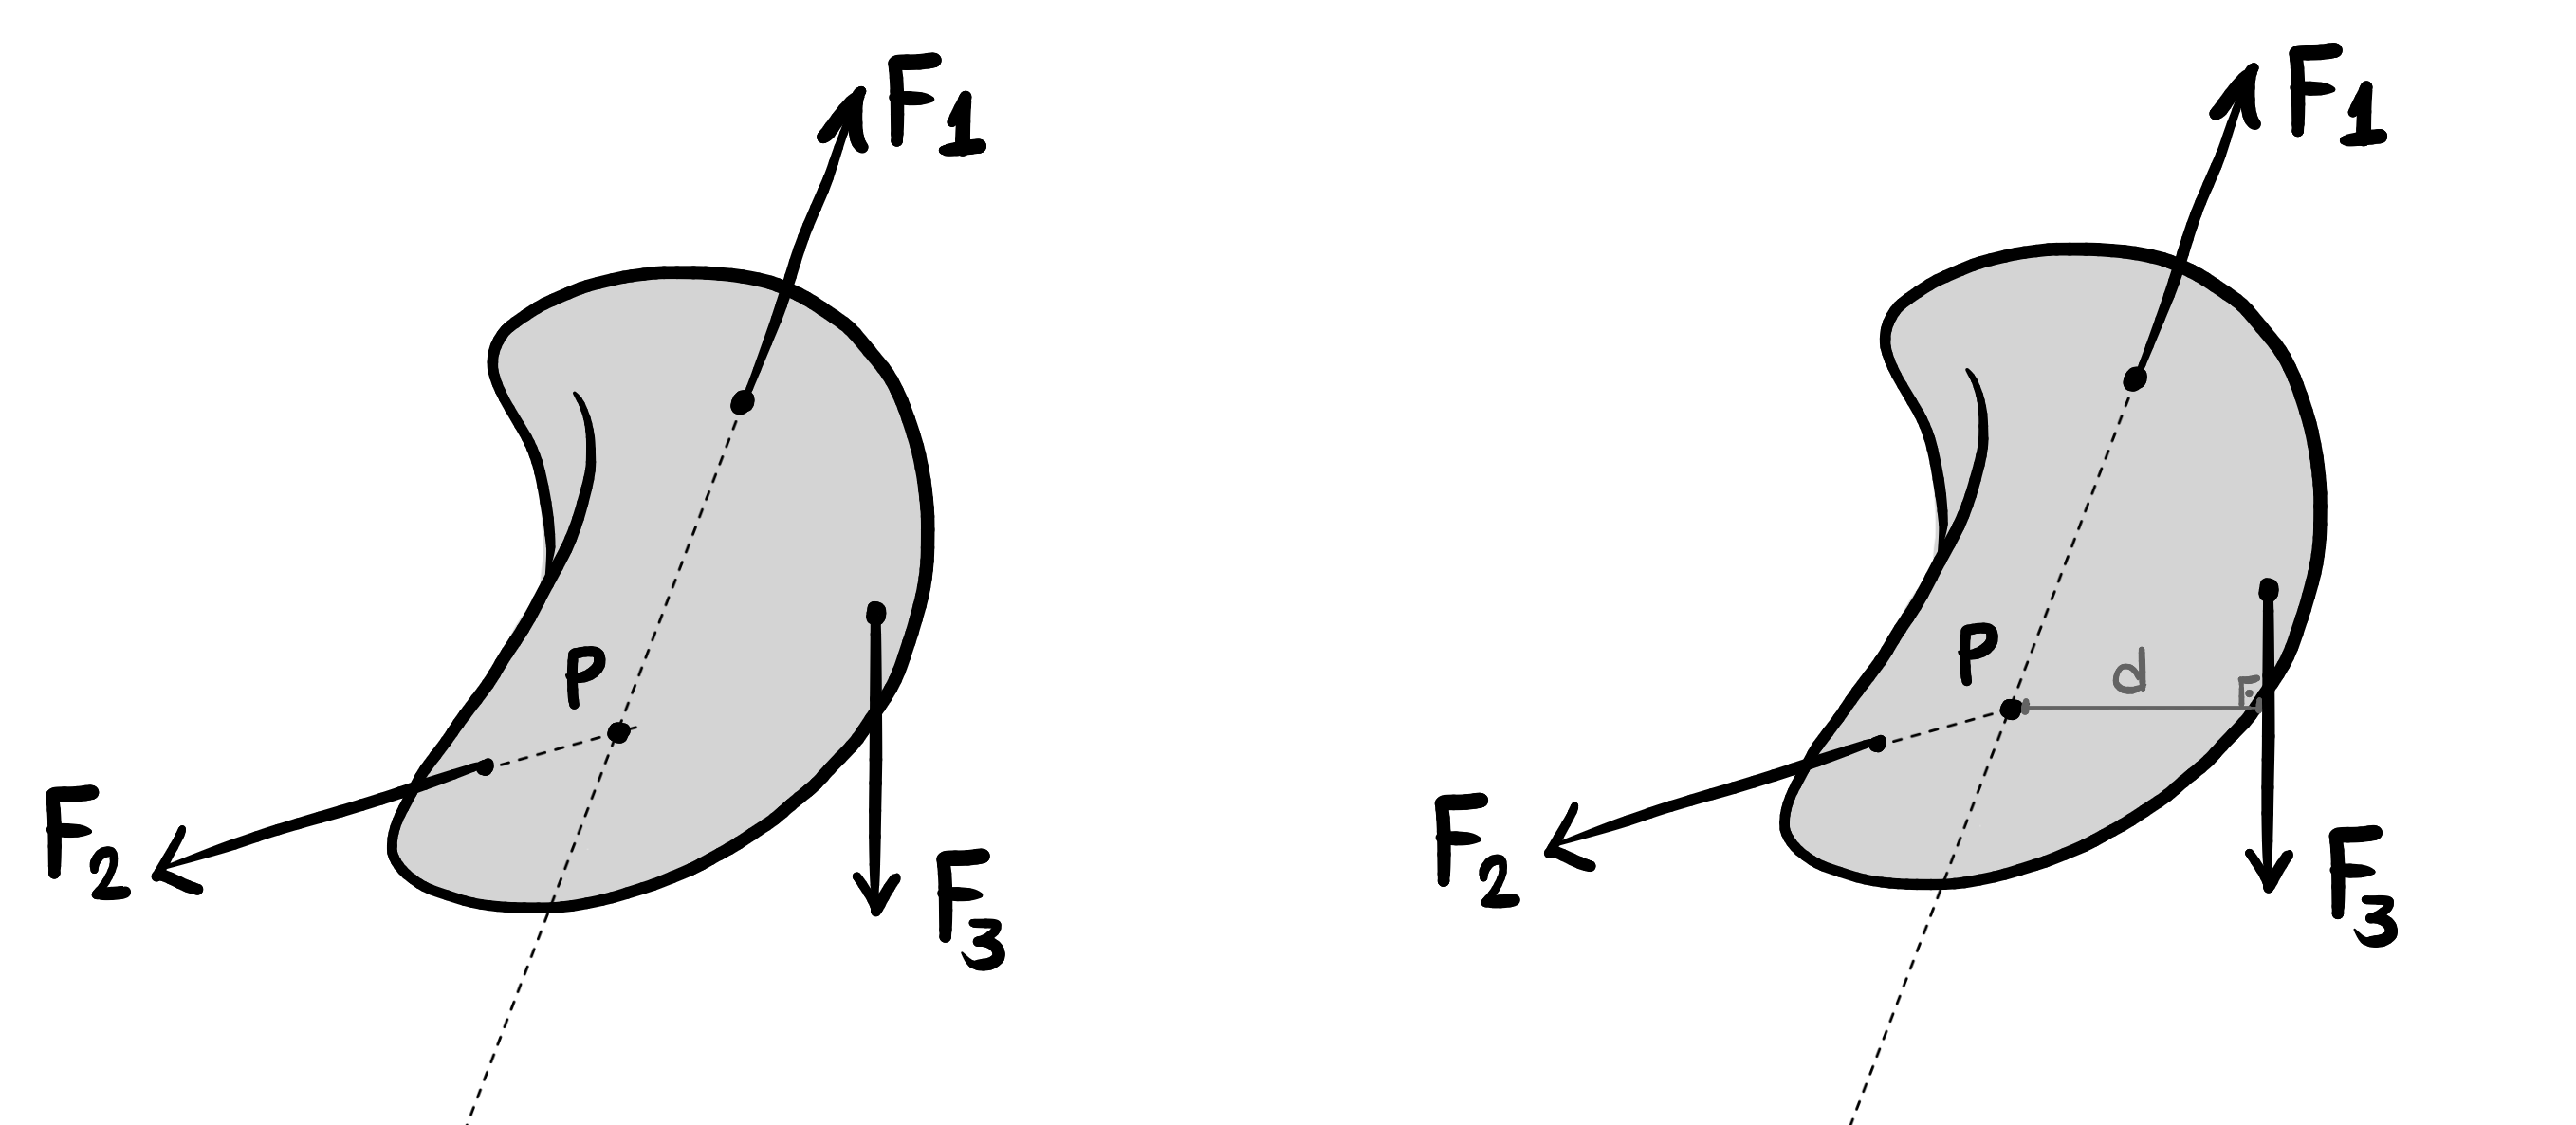
\includegraphics[width=0.7\linewidth]{imagensdinamicarotacao/teorema3forcas.png}};
  \end{scope}
\end{tikzpicture}
\captionof{figure}{Se um corpo extenso está em equilíbrio sob a ação de 3 forças não paralelas elas devem ser concorrentes em um mesmo ponto.}
\label{fig_dinamicarotacao_teorema3forcas}
} 
\vspace{0.3cm}


Além disso, para garantir o equilíbrio de rotação, é preciso que $\tau_\text{R} = 0.$ Tomando os torques em relação ao ponto $P$ vemos que as forças $F_1$ e $F_2$ não gerarão torques, uma vez que elas passam por $P$, ou seja, a distância da sua linha de ação ao ponto $P$ é zero. Assim, é preciso que o torque de $F_3$ em relação a $P$ seja nulo, isto é

$$ \tau_{\text{3}} = F_3 \cdot d = 0 \implies d=0, $$

\noindent ou seja, a distância da linha de ação da força $F_3$ até $P$ deve, também, ser nula, o que prova que as três forças são concorrentes em $P.$ 





\secgfe{Onde é usada}

Em problemas nos quais precisa-se garantir o equilíbrio de um corpo extenso que está sob a ação de exatamente três forças. 

Considere, por exemplo, a situação da primeira imagem da Figura \ref{fig_dinamicarotacao_teorema3forcasporta}, em que lhe é informado como é a força que atua na dobradiça inferior de uma porta, e pergunta-se como é o vetor força na dobradiça superior.



\vspace{0.3cm}
{
\centering
\begin{tikzpicture}
  \begin{scope}[blend mode=multiply]
    \node {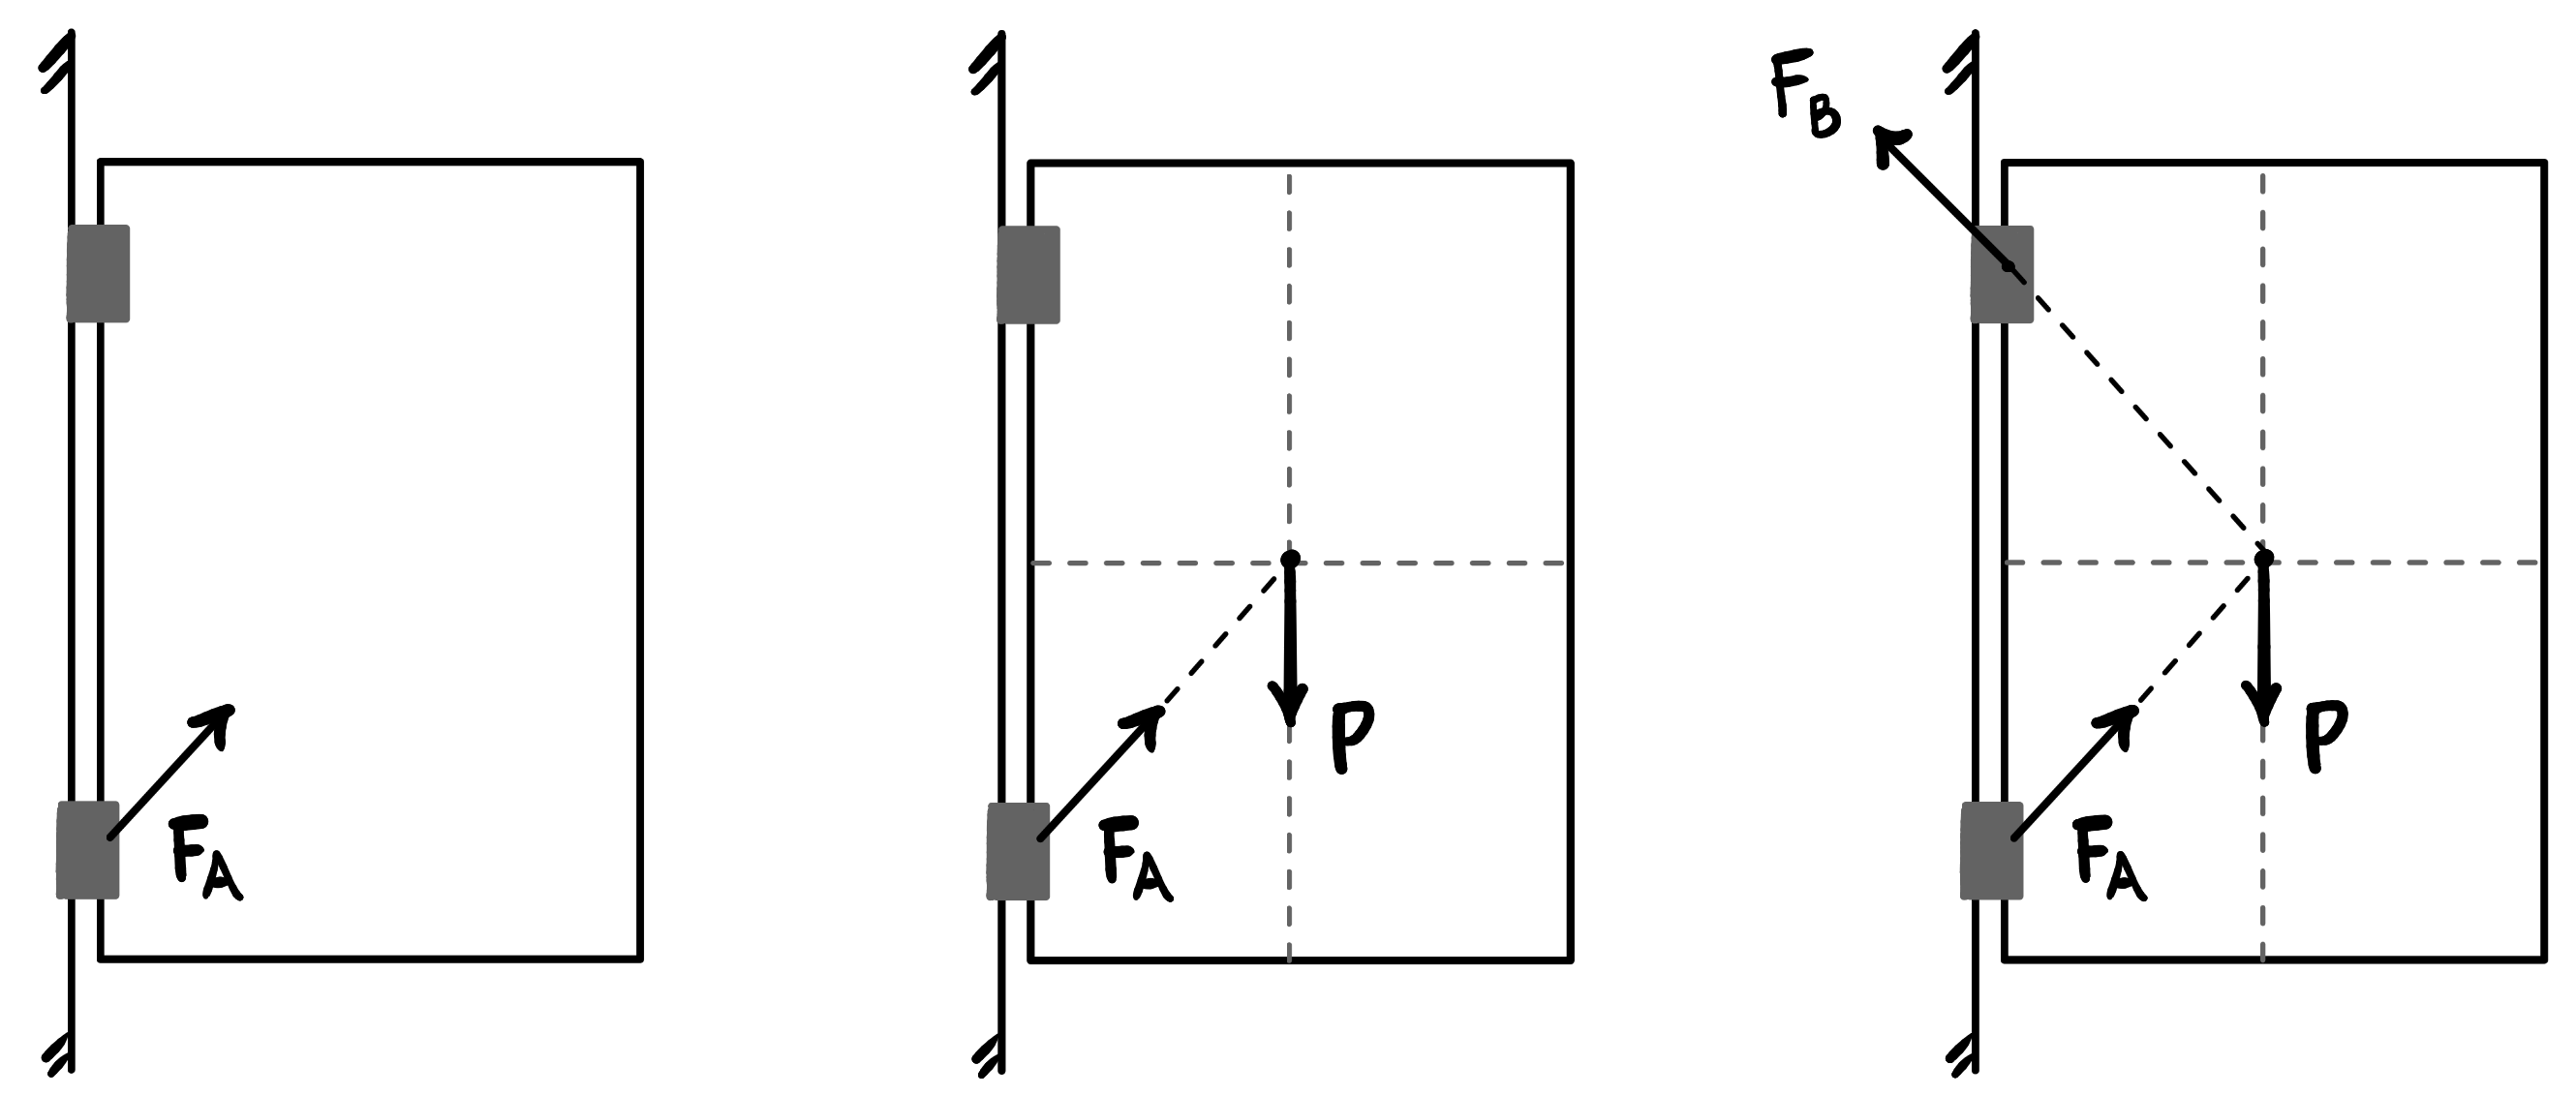
\includegraphics[width=0.6\linewidth]{imagensdinamicarotacao/porta3forcas.png}};
  \end{scope}
\end{tikzpicture}
\captionof{figure}{O teorema das 3 forças nos permite entender para aonde atua a força na dobradiça superior.}
\label{fig_dinamicarotacao_teorema3forcasporta}
} 
\vspace{0.3cm}


Ora, só existem 3 forças atuando na porta: o seu peso e as duas forças que as dobradiças exercem. Como mostra a imagem do meio da figura, o peso e a força na dobradiça inferior já concorrem em um ponto. Assim, se a porta está em equilíbrio, a força na dobradiça superior deve ser tal que sua linha de ação passe por aquele ponto, como mostra a terceira imagem da figura. 

Note que, dada uma direção, a força possui dois sentidos possíveis para os quais pode apontar. O leitor consegue perceber o motivo da força na dobradiça $F_B$ ter exatamente aquele sentido indicado na terceira imagem da Figura \ref{fig_dinamicarotacao_teorema3forcasporta}, e não o sentido contrário?



\secgfe{Erros comuns}

O erro mais comum aqui é o aluno tentar aplicar tal conceito para um corpo que \textbf{não está em equilíbrio,} ou para um corpo no qual atuam mais do que três forças.

É importante ressaltar, portanto, que tal teorema vale, como demonstramos, para corpos em equilíbrio sob a ação de três -- e apenas três -- forças.



\secgfe{Observações}

É interessante observar que, ao obrigar as 3 forças a serem concorrentes, o leitor estará impondo, geometricamente, a condição de equilíbrio de rotação. Retorne à demonstração da Equação \eqref{eq_newtonrotacao_terorema3forcas} e certifique-se de que isso está claro.

Assim, ao resolver um problema de equilíbrio neste contexto, ao impor que as 3 forças são concorrentes, o leitor não precisará escrever que $\tau_\text{R}=0.$ Satisfazer tal condição é análogo a exigir que as 3 forças sejam concorrentes. Sendo assim, a grande vantagem do teorema em questão é trocar um trabalho algébrico (escrever a equação de equilíbrio dos torques) por um trabalho geométrico (impor que os três vetores são concorrentes). Como veremos, em muitos casos essa será uma boa troca e simplificará os cálculos, uma vez que restará apenas exigir que $F_\text{R}=0$ para garantir o equilíbrio total do corpo.


\vspace{0.3cm}


\begin{exemplo}[Nível I]\label{exemplo_dinamicarotacao_teorema3forcasex02}

Considere uma barra homogênea de 6 kg de massa, amarrada por um fio ideal e presa, por um apoio, a uma parede vertical. A Figura \ref{fig_dinamicarotacao_teo3forcasex11} mostra a situação. Se a barra está disposta horizontalmente e se encontra em equilíbrio, qual é o valor da força feita pelo apoio sob a barra? (Considere $\sin \theta = 0.6$ e $\cos \theta = 0.8).$


\vspace{0.3cm}
{
\centering
\begin{tikzpicture}
  \begin{scope}[blend mode=multiply]
    \node {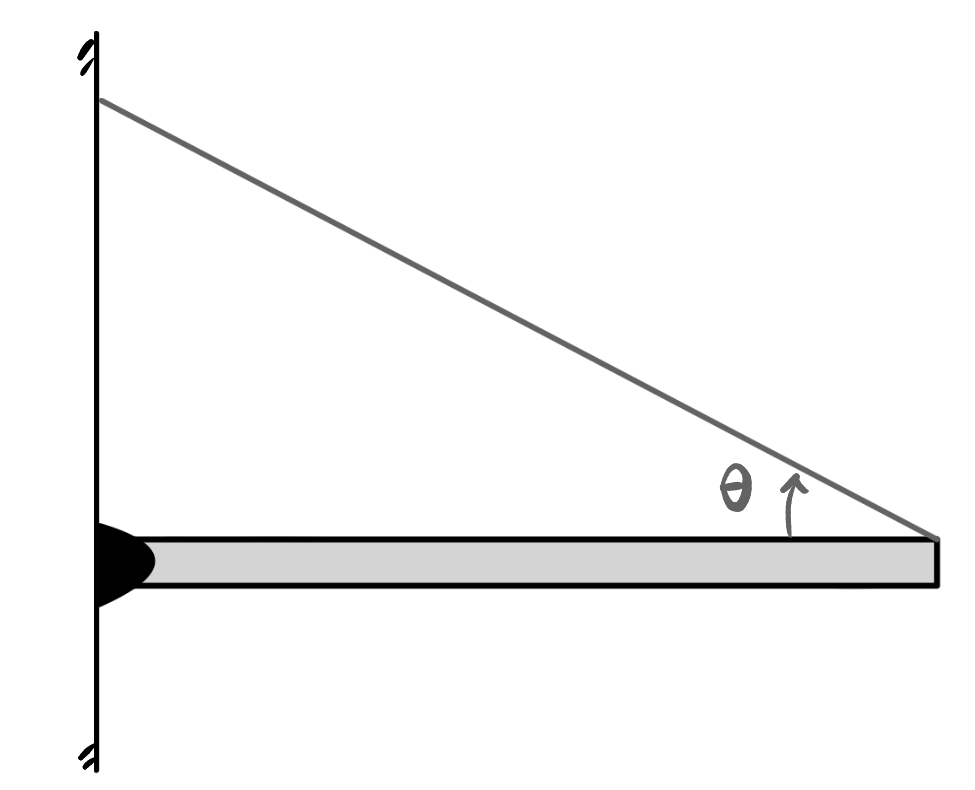
\includegraphics[width=0.3\linewidth]{imagensdinamicarotacao/teo3forcasex11.png}};
  \end{scope}
\end{tikzpicture}
\captionof{figure}{}
\label{fig_dinamicarotacao_teo3forcasex11}
} 
\vspace{0.3cm}


\resolucao

A título de clarear a diferença entre os dois métodos, façamos tal exercício das duas formas que conhecemos.

\begin{enumerate}
    \item Resolvendo da forma tradicional.

    Neste caso, faremos os diagramas das forças e imporemos as condições de equilíbrio, isto é, que as forças se anulam e que os torques se anulam. A Figura \ref{fig_dinamicarotacao_teo3forcasex12} mostra, na primeira imagem, as forças peso e tração que atuam na barra.

\vspace{0.3cm}
{
\centering
\begin{tikzpicture}
  \begin{scope}[blend mode=multiply]
    \node {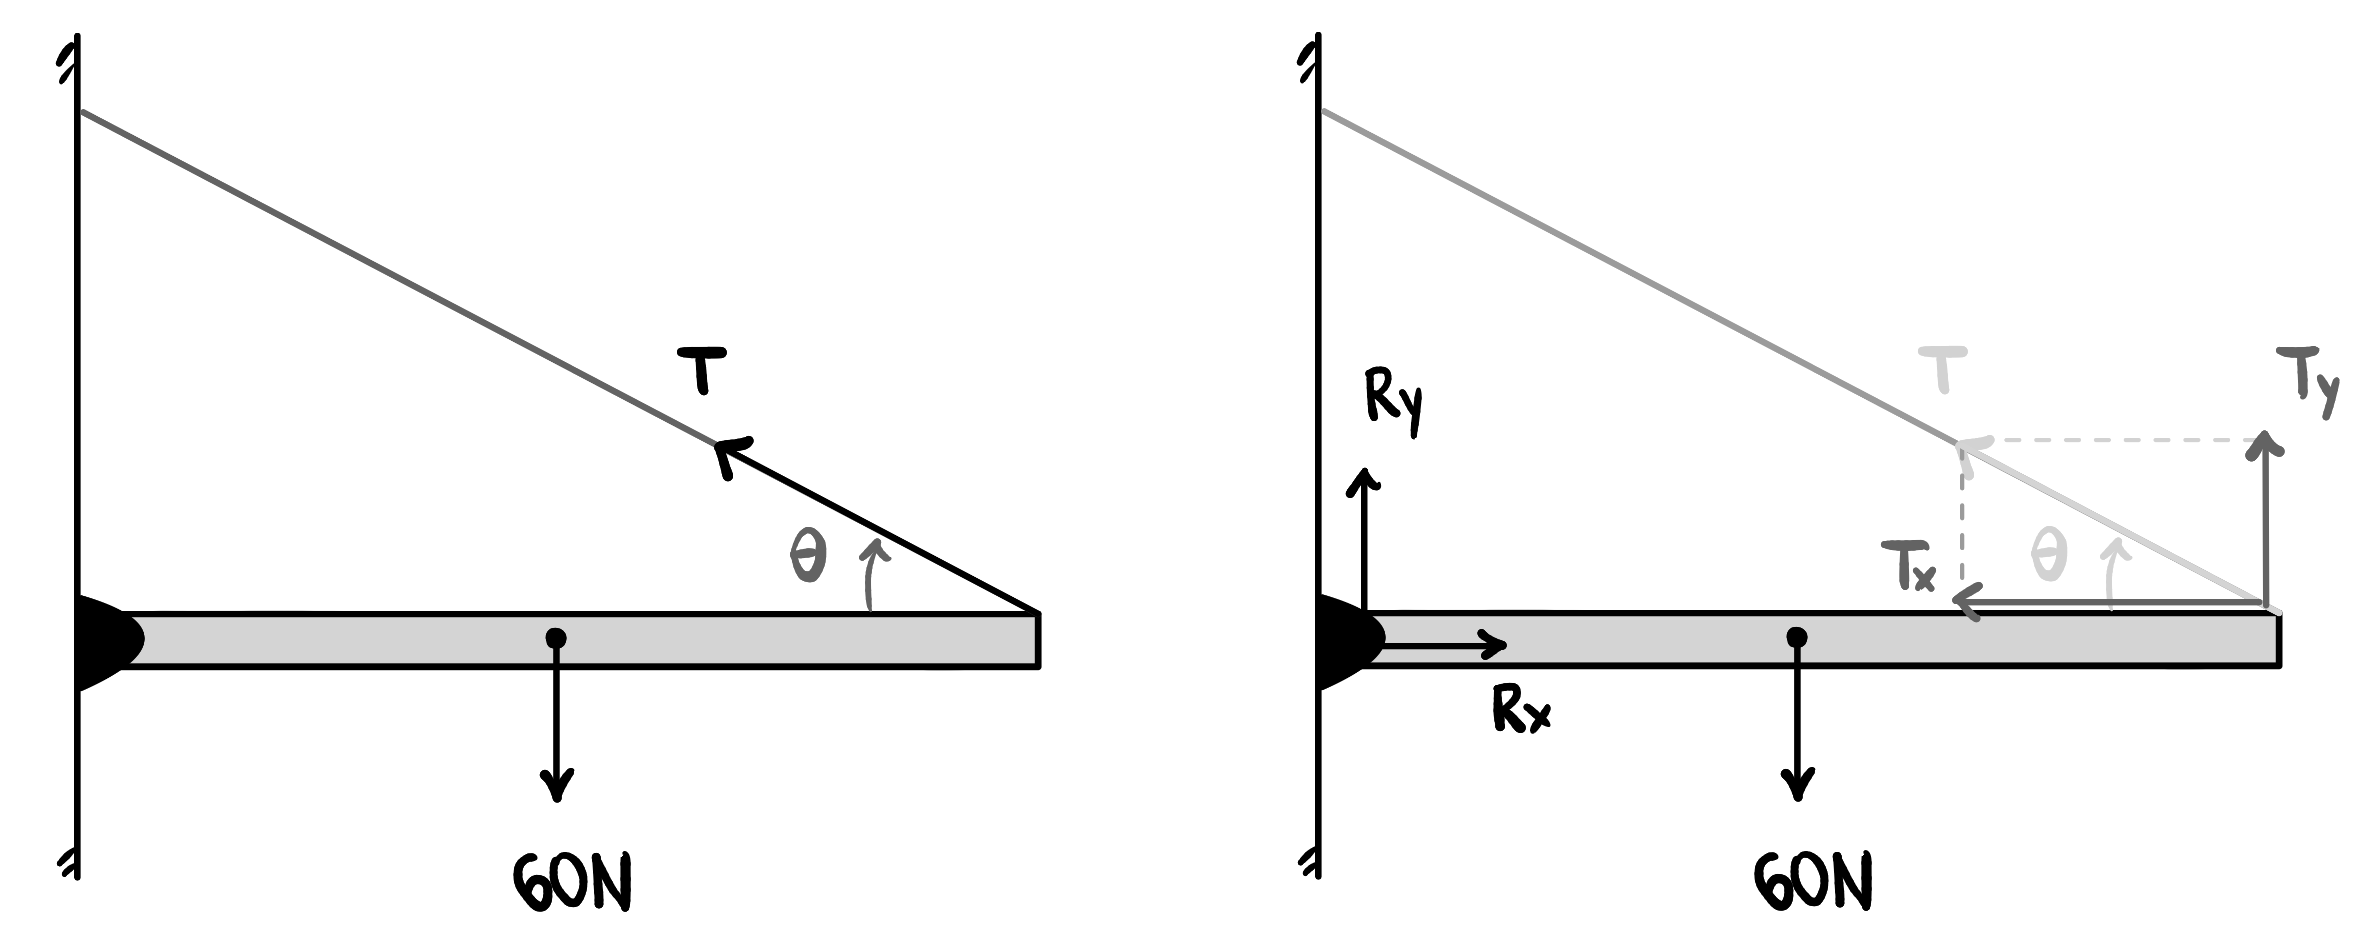
\includegraphics[width=0.75\linewidth]{imagensdinamicarotacao/teo3forcasex12.png}};
  \end{scope}
\end{tikzpicture}
\captionof{figure}{}
\label{fig_dinamicarotacao_teo3forcasex12}
} 
\vspace{0.3cm}

Como não sabemos nada sobre o apoio, sua força de reação pode ser horizontal, vertical, ou oblíqua. Considerando o caso geral, a reação $R$ seria oblíqua, tendo componentes $R_x$ e $R_y.$ Decompondo as forças e impondo as condições de equilíbrio, teremos

$$ \sum F_x = 0 \implies \boxed{R_x = T \sin \theta} \quad \text{ e } \quad \sum F_y = 0 \implies \boxed{R_y = T \cos \theta.} $$

Impondo o equilíbrio de rotação e tomando os torques em relação ao ponto de apoio, teremos:

$$ \tau_{\text{R}_{A}} = 0 \implies 60 \cdot \dfrac{L}{2} = T \sin \theta \cdot L \implies T \sin \theta = 30, $$

\noindent e, como $\sin \theta = 0.6,$ segue que $T = 50$ N. Assim, voltando às equações obtidas do equilíbrio de forças, teremos

$$ R_x = T \sin \theta = 50 \cdot 0.6 \implies \boxed{R_x = 30 \text{ N}}  \text{ | }  R_y = T \cos \theta = 50 \cdot 0.8 \implies \boxed{R_y = 40 \text{ N.}}$$

Assim, pelo Teorema de Pitágoras, teremos que força $R$ do apoio na barra é $R^2 = R_x^2 + R^2_y = 30^2 + 40^2,$ ou seja, $\boxed{R = 50 \text{ N.}}$

\item Pelo teorema das 3 forças.

Neste caso, começamos desenhando as duas forças das quais temos conhecimento: o peso da barra, que atua no seu centro geométrico, e a tração $T$ feita pelo fio, que atua na direção do fio. Isso é o que aparece na primeira imagem da Figura \ref{fig_dinamicarotacao_teo3forcasex13}. Note que essas duas forças já concorrem em um certo ponto. Logo, sabemos que a terceira força deverá, certamente, passar por tal ponto. 

\vspace{0.3cm}
{
\centering
\begin{tikzpicture}
  \begin{scope}[blend mode=multiply]
    \node {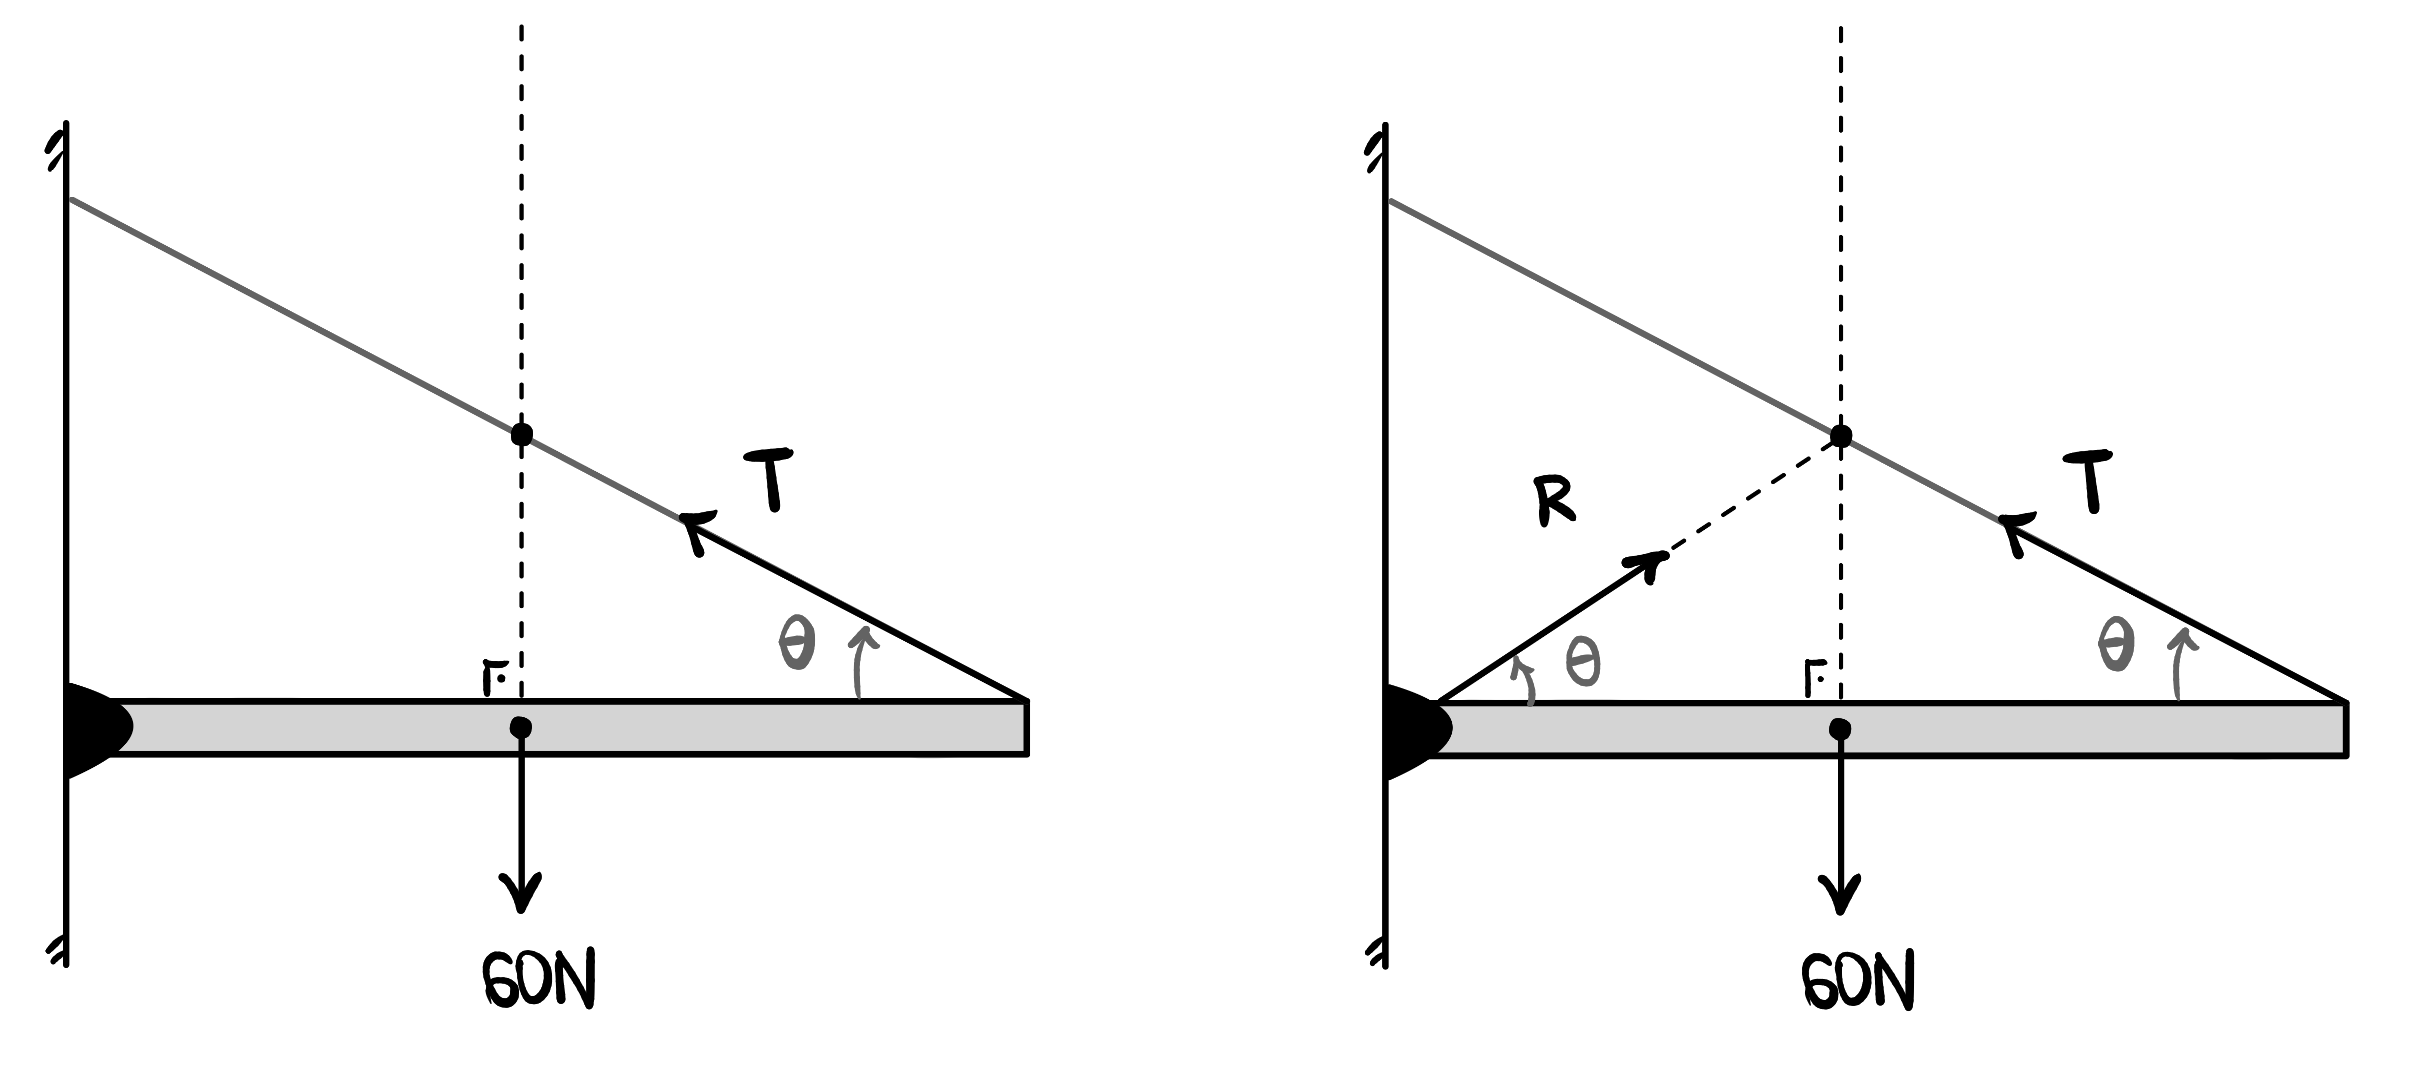
\includegraphics[width=0.75\linewidth]{imagensdinamicarotacao/teo3forcasex13.png}};
  \end{scope}
\end{tikzpicture}
\captionof{figure}{}
\label{fig_dinamicarotacao_teo3forcasex13}
} 
\vspace{0.3cm}

A segunda imagem da figura nos permite obter tal força: traçamos a reta que conecta o ponto de apoio ao ponto no qual as duas outras forças concorrem e a nossa terceira força deve estar nessa direção. Note, contudo, que o triângulo formado pelo fio, pela barra e pela direção da terceira força é isósceles: a sua altura é também mediana, haja vista a homogeneidade da barra. Assim, concluí-se que os ângulos de sua base são iguais. Portanto, por simetria, a força $R$ deve ser exatamente igual à força $T$: $R = T.$

Com isso, para computar a reação $R$ do apoio na barra basta, por exemplo, escrever uma única equação:

$$  F_y = 0 \implies R \sin \theta + T \sin \theta = 60,$$

\noindent em que somamos as componentes verticais de $R$ e $T$, que devem ser anuladas pelo peso da barra. Contudo, sendo $T=R,$ teremos 

$$  R \sin \theta + R \sin \theta = 60 \implies R \sin \theta = 30 \implies R \cdot 0.6 = 30 \implies \boxed{R=50 \text{ N}.}$$

Note que é uma solução algebricamente mais simples: foi preciso impor apenas uma condição de equilíbrio, isto é, que as forças se anulam na vertical. A condição de equilíbrio dos torques é satisfeita uma vez que impomos a condição geométrica das forças concorrem no mesmo ponto -- ela é a versão geométrica da equação de equilíbrio de torques. O anulamento das forças na horizontal é satisfeito de forma imediata uma vez que $R=T$ e que as duas forças são simétricas, isto é, fazem o mesmo ângulo com a barra. Logo, teremos que $T_x=R_x$, e as forças se anulam na horizontal.

    
\end{enumerate}




\end{exemplo}

\vspace{0.3cm}


\begin{exemplo}[Nível II]\label{exemplo_dinamicarotacao_teorema3forcasex02}

Uma barra homogênea de comprimento $\overline{BC}=2\,\text{m}$, se encontra em equilíbrio devido a uma corda de comprimento $\overline{AB}=\sqrt{7}\,\text{m}$ como está representado na figura abaixo. Despreze os atritos, qual é o valor do ângulo $\theta$ formado entre a parede e a barra $\overline{BC}$?

\vspace{0.3cm}

\begin{center}
\begin{tikzpicture}[scale=0.8, line cap=round, line join=round]

    % Pontos
    \coordinate (A) at (0,3.2);
    \coordinate (C) at (0,1.8);
    \coordinate (D) at (0,0.5);   % ponto auxiliar abaixo de C, na parede
    \coordinate (B) at (4.0,0.2);

    % Parede
    \draw[black, line width=0.9pt] (0,-0.8) -- (0,4.4);

    % Fio
    \draw[gray, line width=0.5pt] (A) -- (B);

    % Barra
    \draw[black!70, line width=1.6pt] (C) -- (B);

    % Rótulos
    \node[above right=0.04cm] at (A) {$A$};
    \node[above right=0.04cm] at (C) {$C$};
    \node[right=0.12cm] at (B) {$B$};

    % Ângulo theta
    \draw (C)+(270:0.55) arc[start angle=270,end angle=337,radius=0.55];
    \node at ($(C)+(304:0.9)$) {$\theta$};

\end{tikzpicture}
\end{center}


\resolucao

Inicialmente representamos o peso da barra, no seu centro geométrico, de modo que $\overline{OB} = \overline{OC} = 1 $ m; e a tração no fio. Pelo Teorema das 3 Forças, a terceira força -- aquela que a parede faz na barra -- deve passar por tal ponto. Sabemos que tal força é horizontal, porque, como não há atrito, não haverá componente tangencial de força entre a parede e a barra.


\vspace{0.3cm}
{
\centering
\begin{tikzpicture}
  \begin{scope}[blend mode=multiply]
    \node {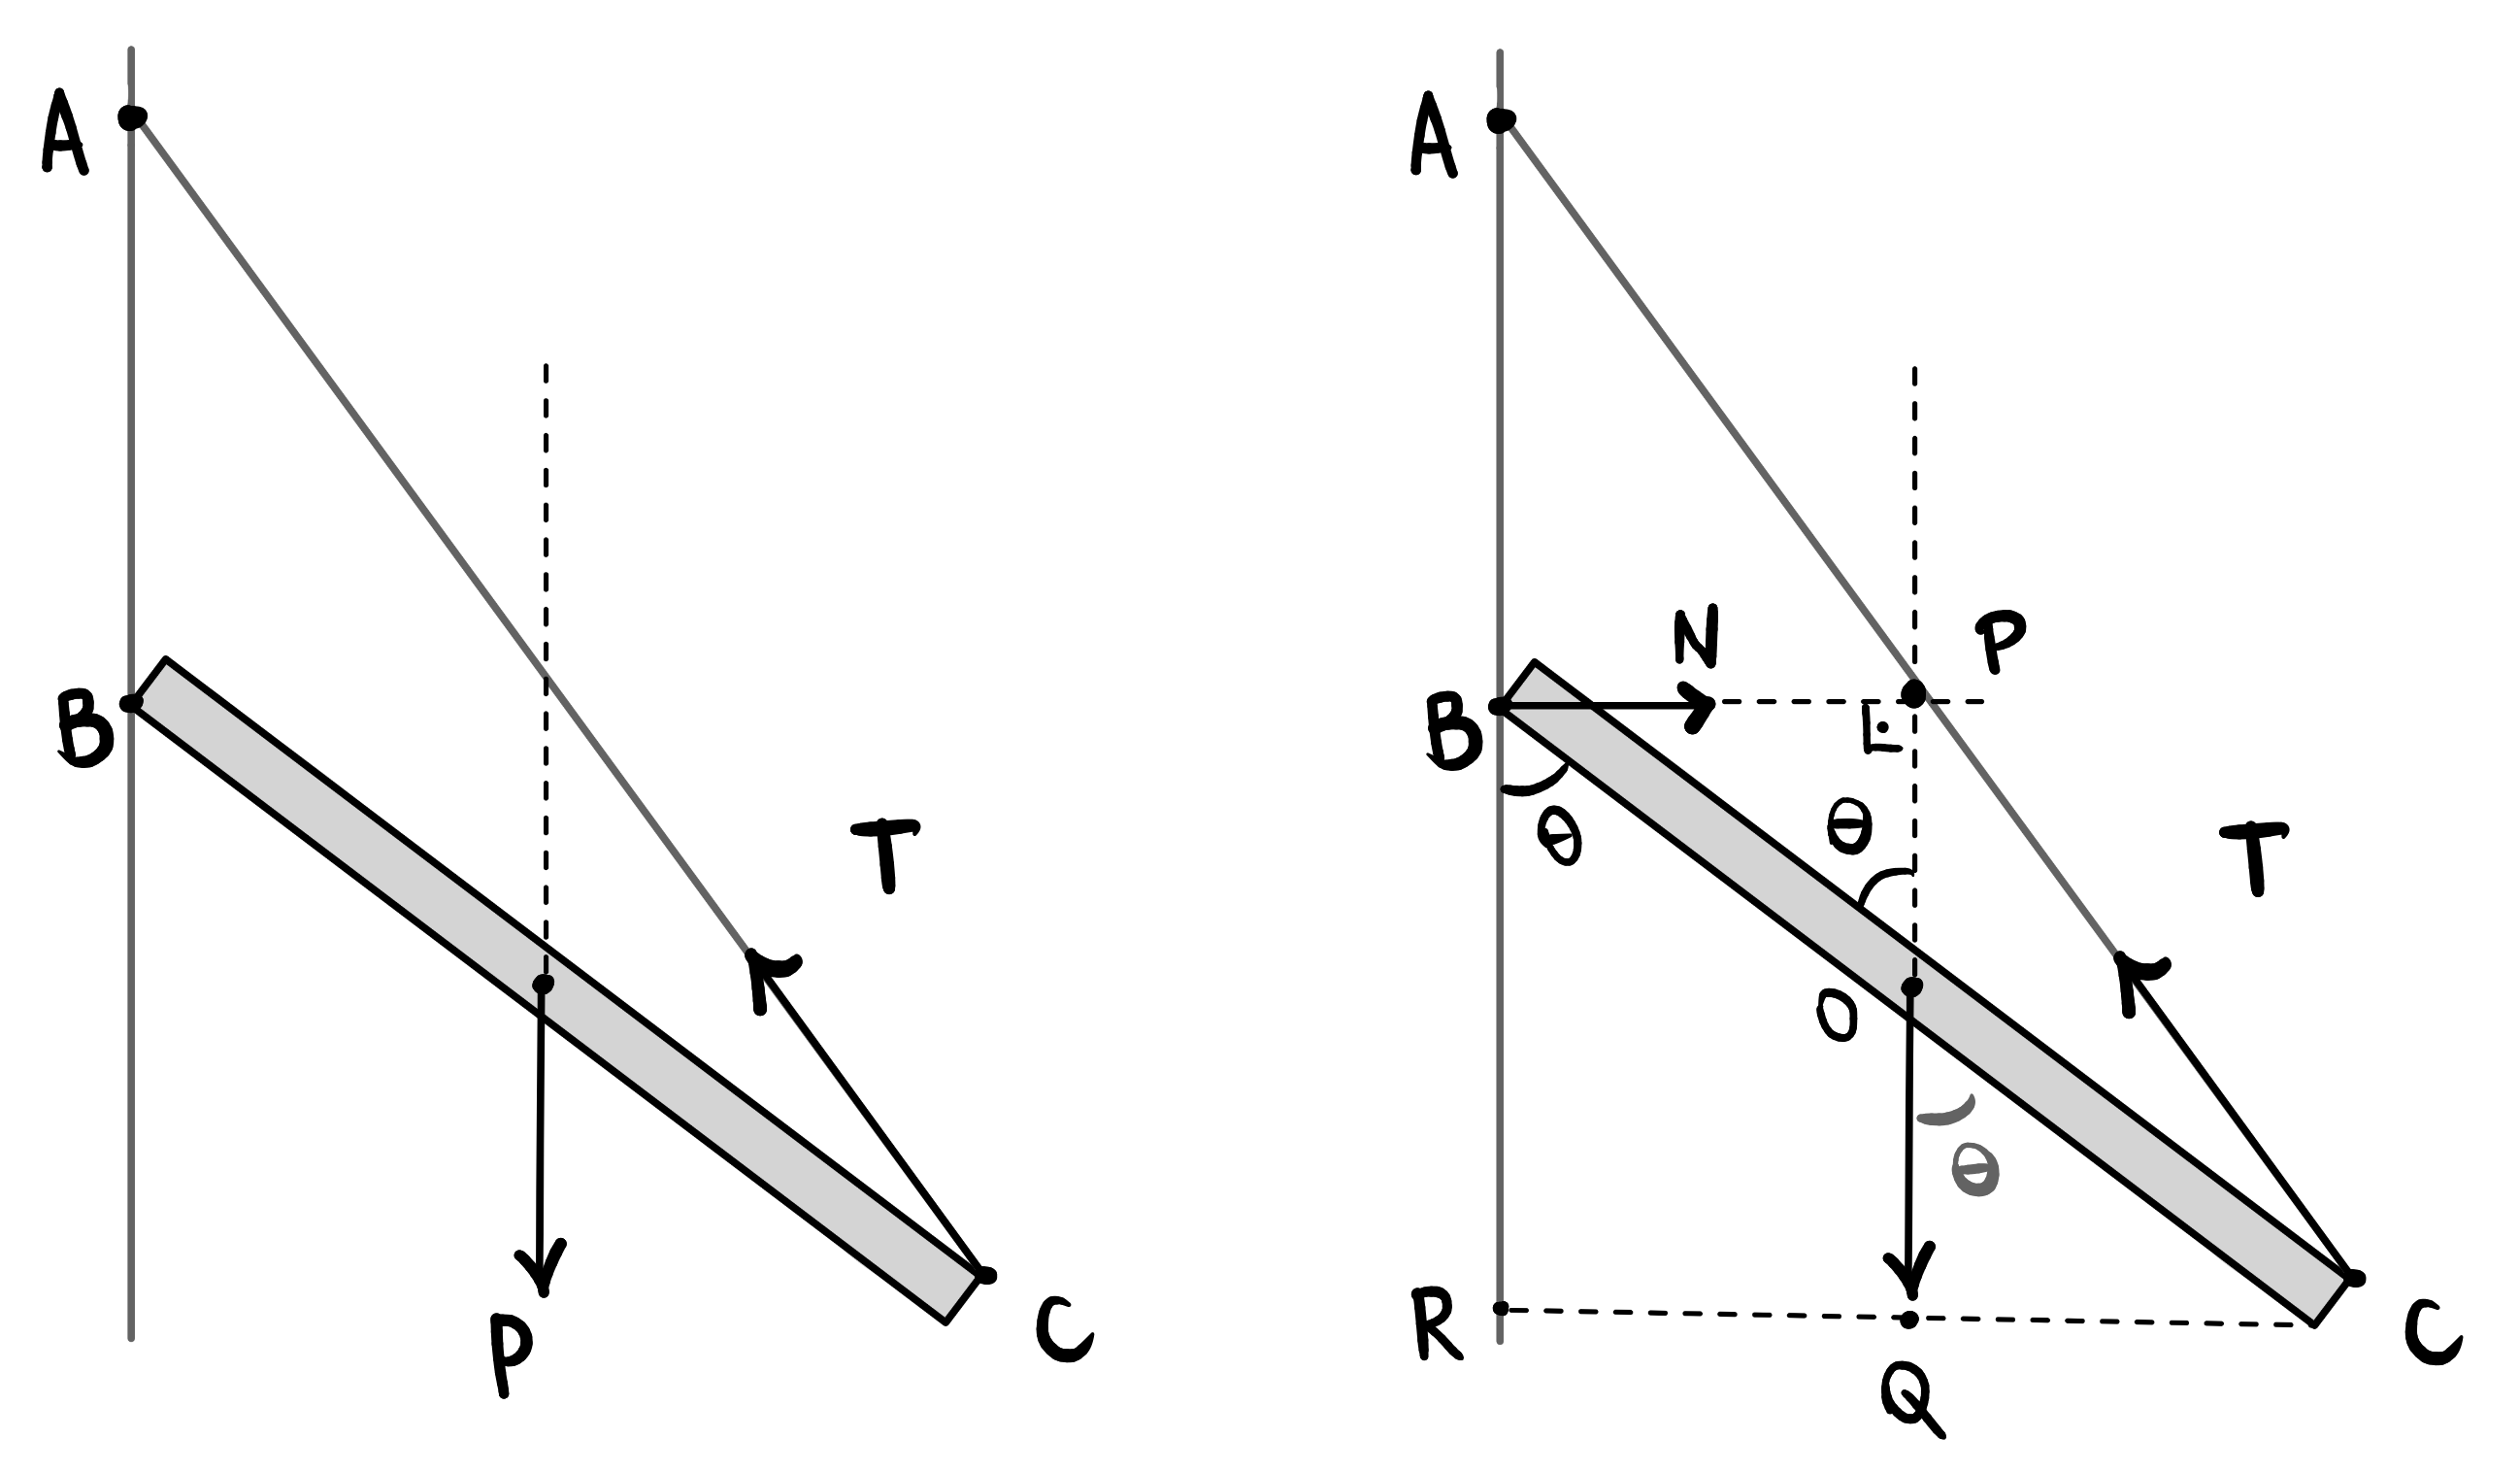
\includegraphics[width=0.7\linewidth]{imagensdinamicarotacao/torqueexemplo02.png}};
  \end{scope}
\end{tikzpicture}
\captionof{figure}{}
\label{fig_dinamicarotacao_torqueexemplo02}
} 
\vspace{0.3cm}

Na segunda imagem da Figura \ref{fig_dinamicarotacao_torqueexemplo02} representamos as três forças concorrendo em $P.$ Perceba, pelo triângulo $OQC$, que 

$$\sin\theta = \dfrac{\overline{QC}}{1} \implies \overline{QC} = \sin \theta.$$ 

Como a reta que passa por $P,$ $O$ e $Q$ corta a barra no seu ponto médio, ela também passará pelo segmento $\overline{RQ}$ em seu ponto médio, ou seja, $\overline{RQ}=\overline{BP} =\overline{QC} = \sin \theta.$ O mesmo vale para o segmento $\overline{AC},$ que será dividido ao meio por tal reta, de modo que $\overline{AP} = \sfrac{\sqrt 7}{2}$.

No triângulo $BRC$ vemos que 

$$ \cos \theta = \dfrac{\overline{BR}}{2} \implies \overline{BR} = 2 \cos \theta.$$

Note, contudo, que o triângulo $ABP$ é congruente ao triângulo $PQC$. Isso ocorre porque eles possuem dois ângulos em comum: o ângulo reto e o ângulo $C\hat PQ = P \hat A C.$ Logo, o terceiro ângulo também há de ser igual, e eles são congruentes. Contudo, como $\overline{BP}=\overline{QC} = \sin \theta,$ a razão de semelhança é 1, e os triângulo são congruentes. Logo, temos $\overline{AB} = \overline{PQ}=\overline{BR}= 2\cos \theta.$

Logo, o problema se resolve pelo Teorema de Pitágoras no triângulo $APB:$

$$ \overline{AP}^2 = \overline{BP}^2 + \overline{AB}^2 \implies \left( \dfrac{\sqrt 7}{2}\right)^2 = \sin^2\theta + (2 \cos \theta)^2.$$

Desenvolvendo e usando que $\sin^2 \theta + \cos^2 \theta =1,$ chegamos que 

$$ \dfrac{7}{4} = 1 + 3 \cos^2 \theta \implies \cos^2 \theta = \dfrac{1}{4} \implies \cos \theta = \dfrac{1}{2},$$

\noindent de onde segue que $\boxed{\theta = 60^\circ.}$


\end{exemplo}

\vspace{0.3cm}


\begin{exemplo}[Nível III - (ITA - 2013)]\label{exemplo_dinamicarotacao_teorema3forcasex03}

Duas partículas, de massas $m$ e $M$, estão respectivamente fixadas nas extremidades de uma barra de comprimento $L$ e massa desprezível. Tal sistema é então apoiado no interior de uma casca hemisférica de raio $r$, de modo a se ter equilíbrio estático com $m$ posicionado na borda $P$ da casca e $M$, num ponto $Q$, conforme mostra a figura. Desconsiderando forças de atrito, a razão $m/M$ entre as massas é igual a

\vspace{0.5cm}

\begin{center}
\begin{tikzpicture}[scale=0.8, line cap=round, line join=round]

    % Parâmetros
    \def\r{3.0}
    \def\angQ{320} % ponto Q na semicircunferência
    \coordinate (O) at (0,0);
    \coordinate (P) at (-\r,0);
    \coordinate (R) at (\r,0);
    \coordinate (Q) at ({\r*cos(\angQ)},{\r*sin(\angQ)});

    % Casca hemisférica
    \draw[line width=1.6pt] (P) arc[start angle=180,end angle=360,radius=\r];

    % Diâmetro tracejado
    \draw[dashed] (P) -- (R);

    % Barra
    \draw[thin] (P) -- (Q);

    % Pontos
    \fill (P) circle (2.4pt);
    \fill (Q) circle (2.4pt);
    \fill (O) circle (2.0pt);

    % Rótulos
    \node[above=3pt] at (P) {$m$};
    \node[left=6pt] at (P) {$P$};
    \node[above=4pt] at (O) {$O$};
    \node[above=4pt] at ($(O)!0.55!(R)$) {$r$};
    \node[right=5pt] at (Q) {$Q$};
    \node[above=4pt] at (Q) {$M$};

    % Rótulo L sobre a barra
    \node at ($(P)!0.48!(Q)+(0,-0.35)$) {$L$};

\end{tikzpicture}
\end{center}

\vspace{0.4cm}

\begin{enumerate}
    \item[(a)] $\dfrac{L^2-2r^2}{2r^2}$
    
    \item[(b)] $\dfrac{2L^2-3r^2}{2r^2}$
    
    \item[(c)] $\dfrac{L^2-2r^2}{r^2-L^2}$
    
    \item[(d)] $\dfrac{2L^2-3r^2}{r^2-L^2}$
    
    \item[(e)] $\dfrac{3L^2-2r^2}{L^2-2r^2}$
\end{enumerate}


\resolucao

Este é um problema que se resolve de forma extremamente elegante usando o Teorema das 3 Forças. Para tal, consideraremos a barra como um corpo único, com o seu peso total $P=(m+M)g$ atuando no seu centro de massa. Considerando como origem a posição da massa $m$, e sendo o eixo $x$ orientado ao longo da barra, a posição do centro de massa é 

$$ x_\text{CM} = \dfrac{m \cancelto{0}{x_1} + Mx_2}{m+M} = \dfrac{ML}{m+M}.$$

Dado isso, apenas três forças atuarão na barra: as normais feitas pelo hemisfério nos pontos $P \text{ e } Q$ e o seu peso total, atuando no seu centro de massa, localizado no ponto $C$, conforme pode-se ver na primeira imagem da Figura \ref{fig_dinamicarotacao_ita2013teorema3forcas}. 

\vspace{0.3cm}
{
\centering
\begin{tikzpicture}
  \begin{scope}[blend mode=multiply]
    \node {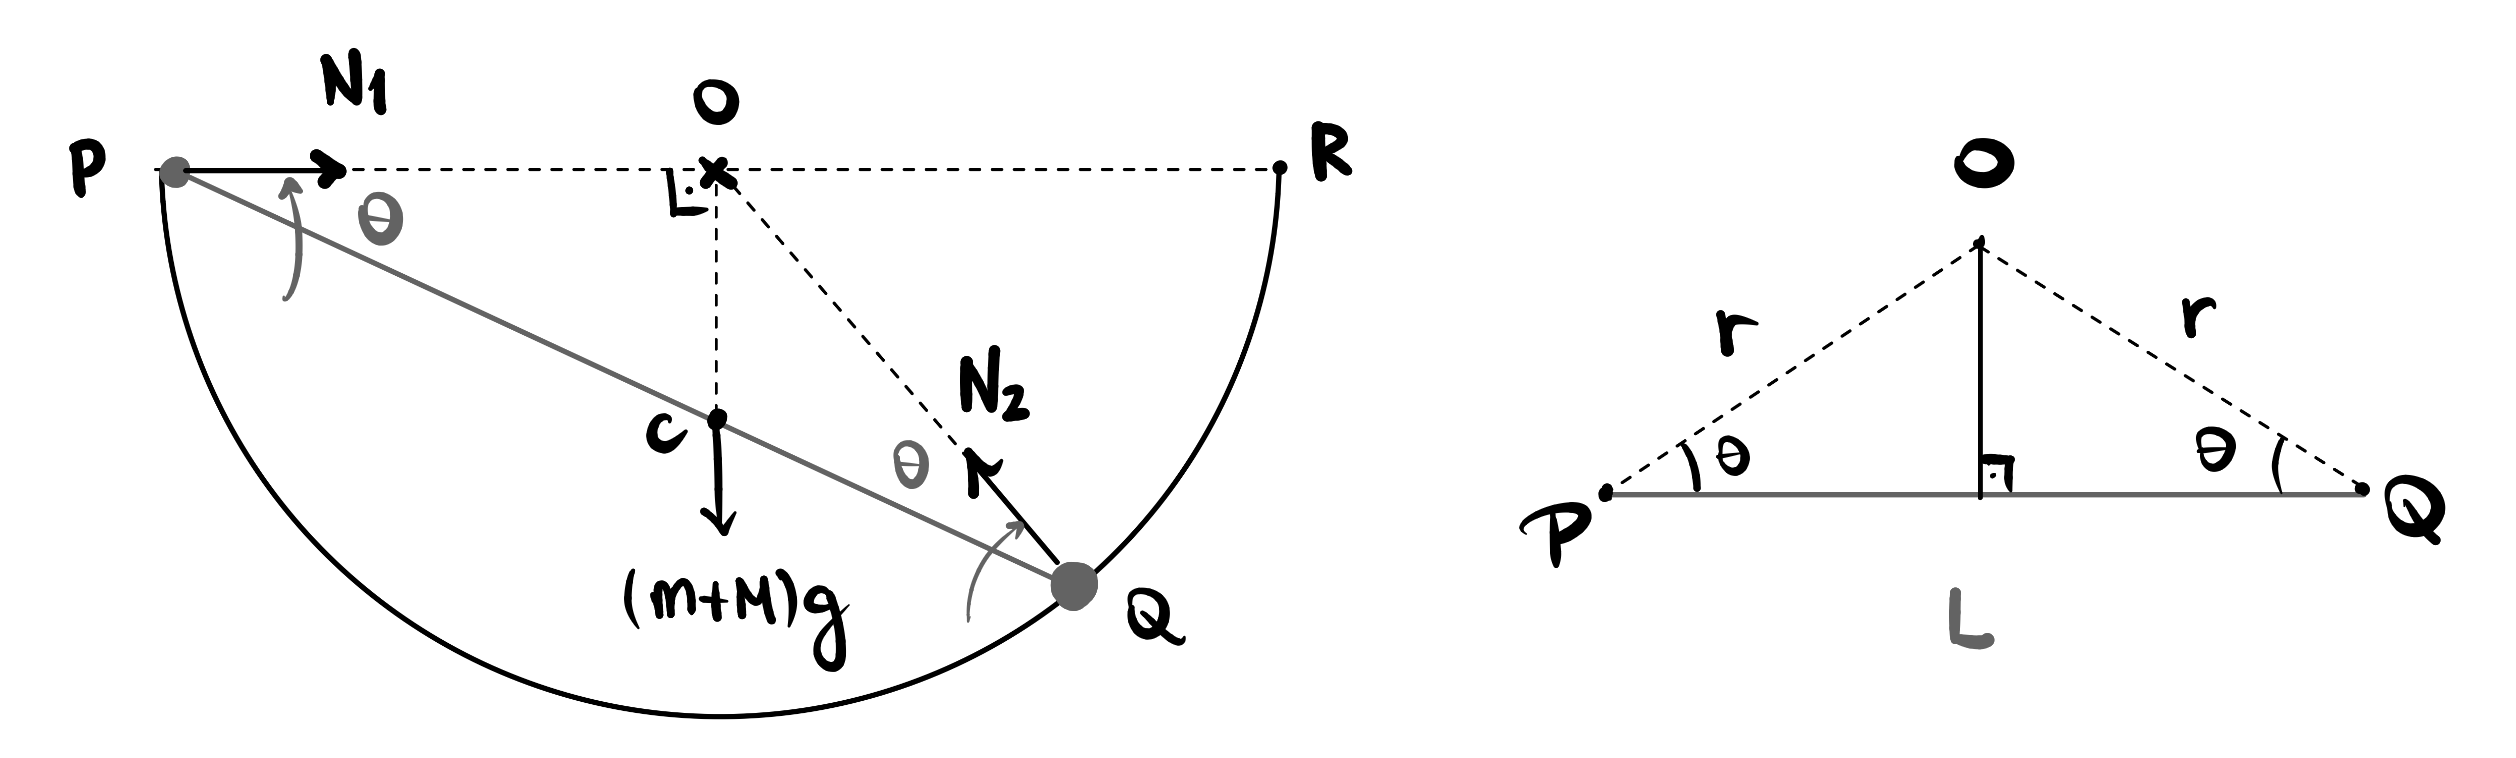
\includegraphics[width=0.75\linewidth]{imagensdinamicarotacao/ita2013teorema3forcas.png}};
  \end{scope}
\end{tikzpicture}
\captionof{figure}{}
\label{fig_dinamicarotacao_ita2013teorema3forcas}
} 
\vspace{0.3cm}

As três forças já foram desenhadas de modo a concorrem em $O,$ o que já garante o equilíbrio de rotação. Observando a primeira imagem da figura, vemos que $\overline{PC} = x_\text{CM}.$ Pela definição de cosseno no triângulo $POC$ tem-se

$$ \cos \theta = \dfrac{\overline{PO}}{\overline{PC}} = \dfrac{r}{\dfrac{ML}{m+M}}.$$

Note que o triângulo $POQ$ é isósceles, haja vista que $\overline{PO} = \overline{QO}=r.$ Assim, os ângulos da sua base são iguais. A imagem da direita destaca esse triângulo, em que, também usando a definição de cosseno, vemos que

$$ \cos \theta = \dfrac{\dfrac{L}{2}}{r} = \dfrac{L}{2r}.$$

Igualando as duas últimas expressões que fornecem $\cos \theta,$ somos levados a

$$ \dfrac{r}{\dfrac{ML}{m+M}} = \dfrac{L}{2r} \implies \dfrac{m+M}{M} = \dfrac{L^2}{2r^2} \implies \dfrac{m}{M} + 1 =  \dfrac{L^2}{2r^2} \implies \boxed{\dfrac{m}{M} = \dfrac{L^2-2r^2}{2r^2}  \text{ (letra A)}.}$$


\end{exemplo}


\vspace{0.3cm}








\begin{secnivel}[Momento angular]{III}{Momento angular}
 

  \eqLdois{def}{eq_momento_angular}{L = mvr \sin \theta}
  

\end{secnivel}


%  O momento angular de uma partícula de massa $m$, velocidade $v$ e distância $r$ em relação ao ponto $O$ é:
% em que $\theta$ é o ângulo entre o vetor velocidade $\vec v$ e o vetor posição $\vec r.$

\secgfe{De onde vem}


A Segunda Lei de Newton, na versão expressa pela Equação \eqref{eq_newton_segundaleisistemaparticulas}, diz que a força resultante tem o papel de alterar o momento linear de um corpo (ou sistema de corpos):

\begin{equation}
     F_\text{R} = \dfrac{\Delta p}{\Delta t}.
    \label{eq_rotacao_segundaleinewtonoriginal}
\end{equation}

Já vimos que existe uma grandeza associada a uma força $F$ responsável por medir a capacidade que tal força tem de produzir rotação em torno de um certo ponto. Tal grandeza é o torque $\tau,$ definido pela Equação \eqref{eq_newton_torque}. Será que existe algo análogo à Segunda Lei de Newton expressa na Equação \eqref{eq_rotacao_segundaleinewtonoriginal}, porém para grandezas rotacionais?

A resposta é sim, e isso acabará desaguando em uma nova grandeza. Considere, por exemplo, a situação da Figura \ref{fig_gravitacao_momentoangulardefinicao1}, que mostra duas partículas de mesma massa $m$ e velocidade $v$, girando em torno de um centro $O,$ porém uma delas em uma circunferência com o dobro do raio da primeira. Qual das duas partículas possui maior inércia rotacional? Isto é, qual delas é mais difícil de parar, mudar de trajetória ou fazer girar mais depressa -- ou seja, qual possui maior tendência de permanecer em seu estado de movimento rotacional?

\vspace{0.3cm}
{
\centering
\begin{tikzpicture}
  \begin{scope}[blend mode=multiply]
    \node {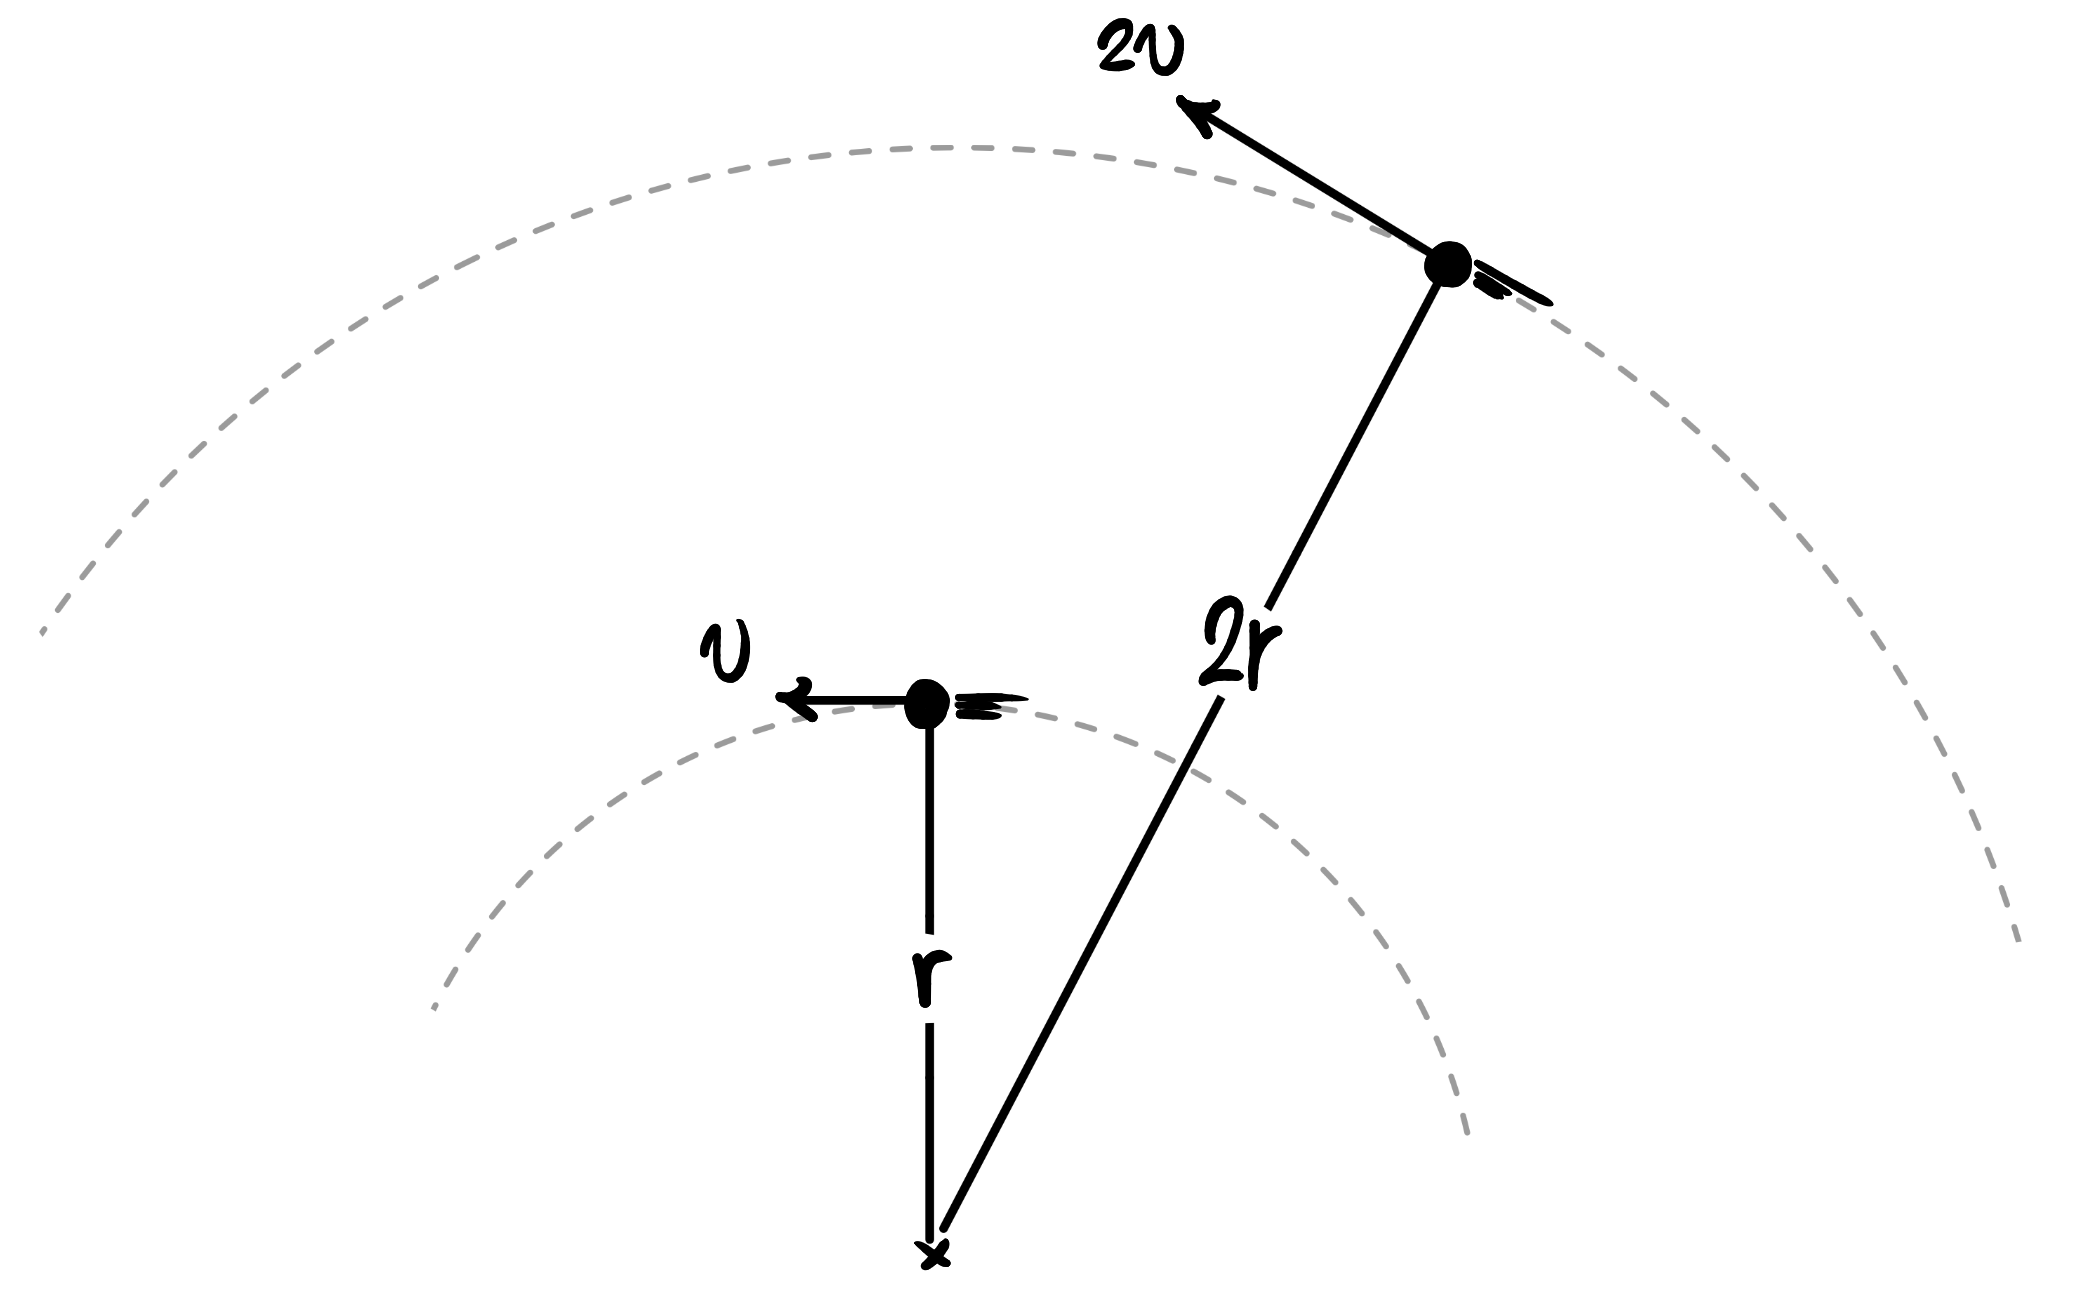
\includegraphics[width=0.5\linewidth]{imagensgravitacao/momentoangulardefinicao1.png}};
  \end{scope}
\end{tikzpicture}
\captionof{figure}{A inércia de rotação.}
\label{fig_gravitacao_momentoangulardefinicao1}
} 
\vspace{0.3cm}

Perceba que, para fazer qualquer uma das duas partículas aumentar a velocidade em uma certa quantidade, tendo elas a mesma massa, será necessária a mesma aceleração $a$, o que exigirá exatamente a mesma força $F$ atuando ao longo do mesmo intervalo de tempo. Contudo, esse é um raciocínio voltado para grandezas lineares, e queremos pensar nas grandezas angulares (rotacionais). Note que a mesma força $F$, tangencial, realizada sobre a partícula $A,$ de órbita com raio $2r$, irá gerar o dobro do torque $\tau$ do que a mesma força aplicada na partícula $B,$ de órbita circular de raio $r$:

$$ \tau_\text{A} = F \cdot (2r) = 2 (F \cdot r) = 2 \tau_\text{B}.$$
 
Logo, para fazer a partícula $A$ girar mais depressa (ou mais devagar) é necessário o dobro de torque para alterar seu ``movimento rotacional.'' Mas o que seria essa ``quantidade de movimento rotacional,'' ou ``momento linear de rotação?'' Seria a grandeza que varia sob a ação de torques. Partindo da Equação \eqref{eq_rotacao_segundaleinewtonoriginal} e multiplicando por $r$ dos dois lados,\footnote{A grandeza $r$ aqui seria o raio de rotação, ou seja, o nosso braço de alavanca: a distância do ponto de aplicação da força até o ponto em relação ao qual tomam-se os torques, que vem a ser o centro de rotação no caso da Figura \ref{fig_gravitacao_momentoangulardefinicao1}.} teremos:

$$ F_\text{R} \cdot r = \dfrac{\Delta p}{\Delta t} \cdot r  \implies \tau_\text{R} = \dfrac{\Delta (p \cdot r)}{\Delta t},$$

\noindent ou seja, essa espécie de ``Segunda Lei de Newton rotacional'' diz que, tal como o efeito da força é variar o momento linear $p,$ o efeito do torque é variar o momento angular $L=p\cdot r.$ Desse modo, podemos enxergar o momento angular como sendo o análogo do momento linear, porém para rotações.

Assim, a equação final acima se escreverá

$$ \tau_\text{R} = \dfrac{\Delta L}{\Delta t},$$

\noindent isto é, o efeito resultante dos torques externos é variar o momento angular $L$ da partícula. Logo, em um sistema ou contexto em que o torque externo é nulo, o momento angular $L$ é uma grandeza que se conserva.

Note que, neste sentido, o momento angular $L$ ficou sendo simplesmente o produto do momento linear $p$ pelo braço de alavanca $r$, isto é, $L= p \cdot r = mvr,$ uma espécie de ``momento linear rotacional.'' Contudo, este será o caso apenas quando a velocidade $v$ for perpendicular ao raio de rotação $r,$ como foram os casos da Figura \ref{fig_gravitacao_momentoangulardefinicao1}.

De modo geral, a velocidade pode não ser perpendicular a tal raio, como seria o caso de uma órbita elíptica de um satélite sob a ação do campo gravitacional. Neste caso, como mostra a Figura \ref{fig_gravitacao_momentoangulardefinicao2}, o ângulo entre a direção de $r$ e o vetor velocidade $v$ é $\theta.$ Como queremos computar a ``quantidade de movimento rotacional,'' decompomos a velocidade $v$ e pegamos sua componente $v_\perp,$ isto é, sua componente perpendicular ao braço de alavanca $r,$ que seria a componente da força responsável por uma rotação pura em torno do ponto em relação ao qual tomamos os torques (ponto no qual se encontra a massa central, no caso gravitacional).


\vspace{0.3cm}
{
\centering
\begin{tikzpicture}
  \begin{scope}[blend mode=multiply]
    \node {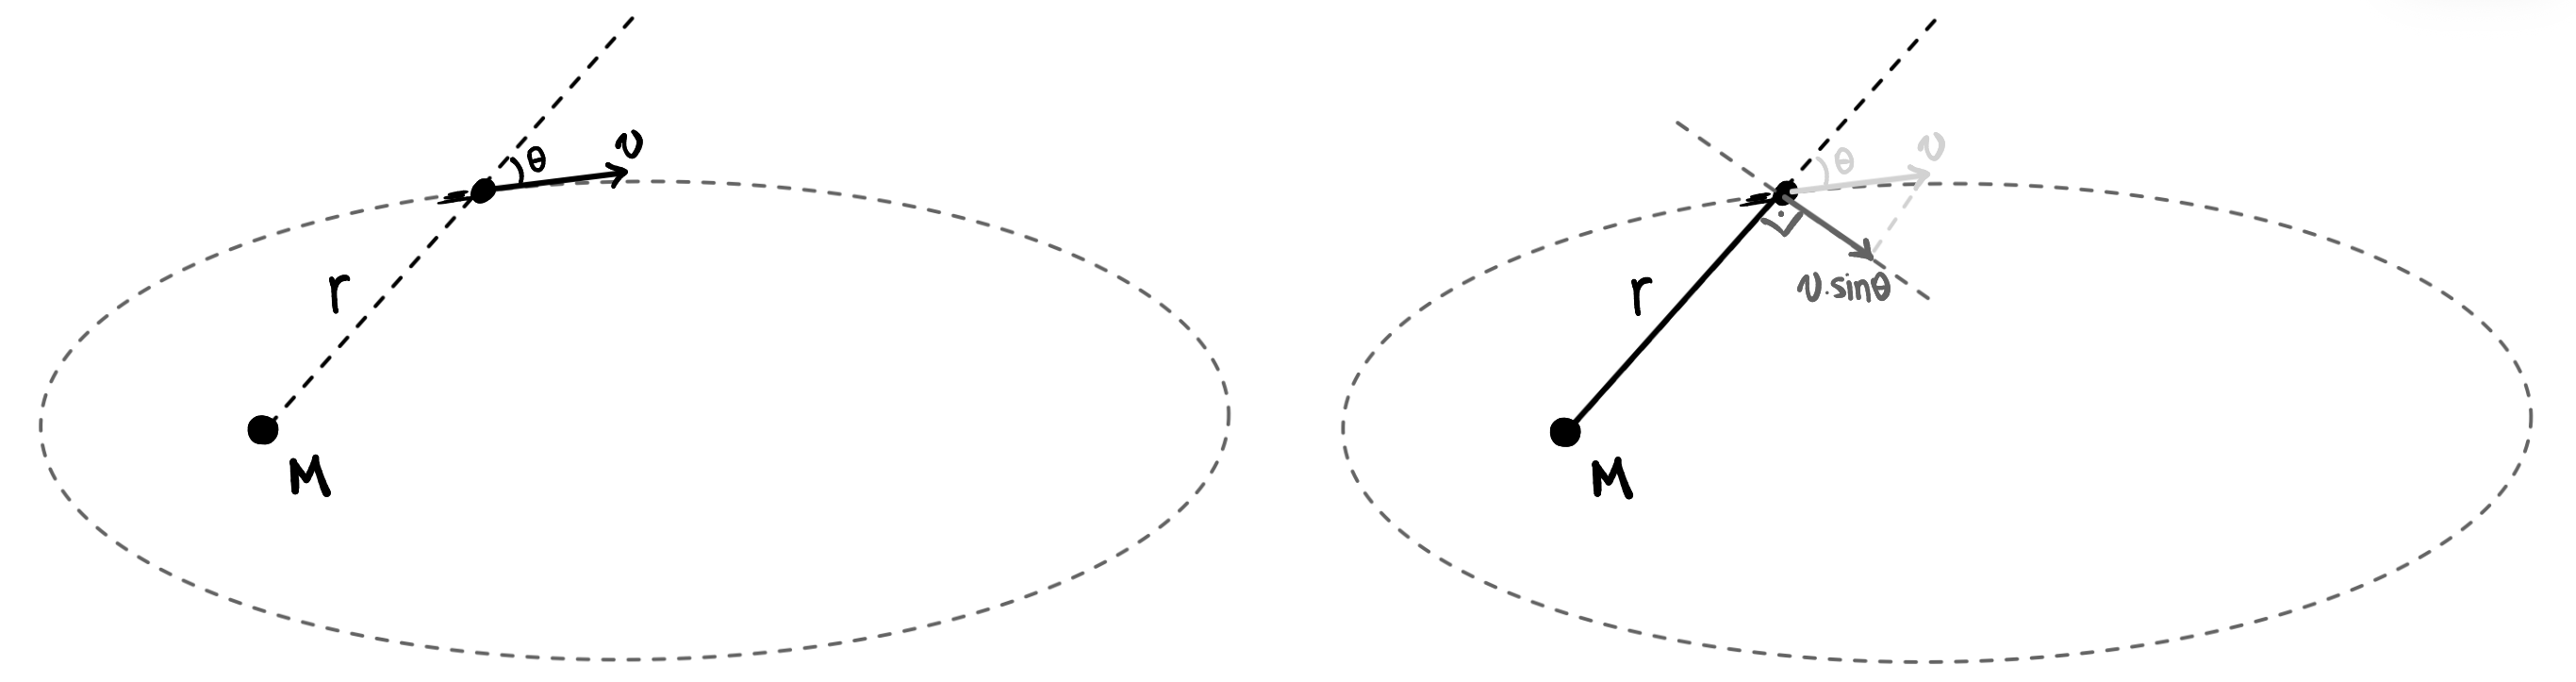
\includegraphics[width=1.0\linewidth]{imagensgravitacao/momentoangulardefinicao2.png}};
  \end{scope}
\end{tikzpicture}
\captionof{figure}{O momento angular $L$ é dado pelo produto da componente de velocidade rotacional $v_\perp = v \sin \theta$ pelo braço de alavanca $r.$}
\label{fig_gravitacao_momentoangulardefinicao2}
} 
\vspace{0.3cm}


Assim, o momento angular $L$ é, tal como no caso do torque, o produto da componente rotacional do momento linear,, isto é, $p_\perp = mv_\perp = mv \sin \theta,$ pelo braço de alavanca $r,$ que se expressa na Equação \eqref{eq_momento_angular}.


\secgfe{Onde é usada}

Os casos mais comuns de aplicação do conceito e do cálculo de momento angular são situações em que tal grandeza se conserva. As mais comuns serão aquelas em que o torque externo é nulo, o que sempre acontece quando um corpo está sob ação de uma força central, como a força gravitacional.

Um caso bastante comum de aplicação é o da órbita elíptica de um corpo em torno de outro, sob a ação do campo gravitacional. A Figura \ref{fig_gravitacao_forcacentral} mostra essa situação.

\vspace{0.3cm}
{
\centering
\begin{tikzpicture}
  \begin{scope}[blend mode=multiply]
    \node {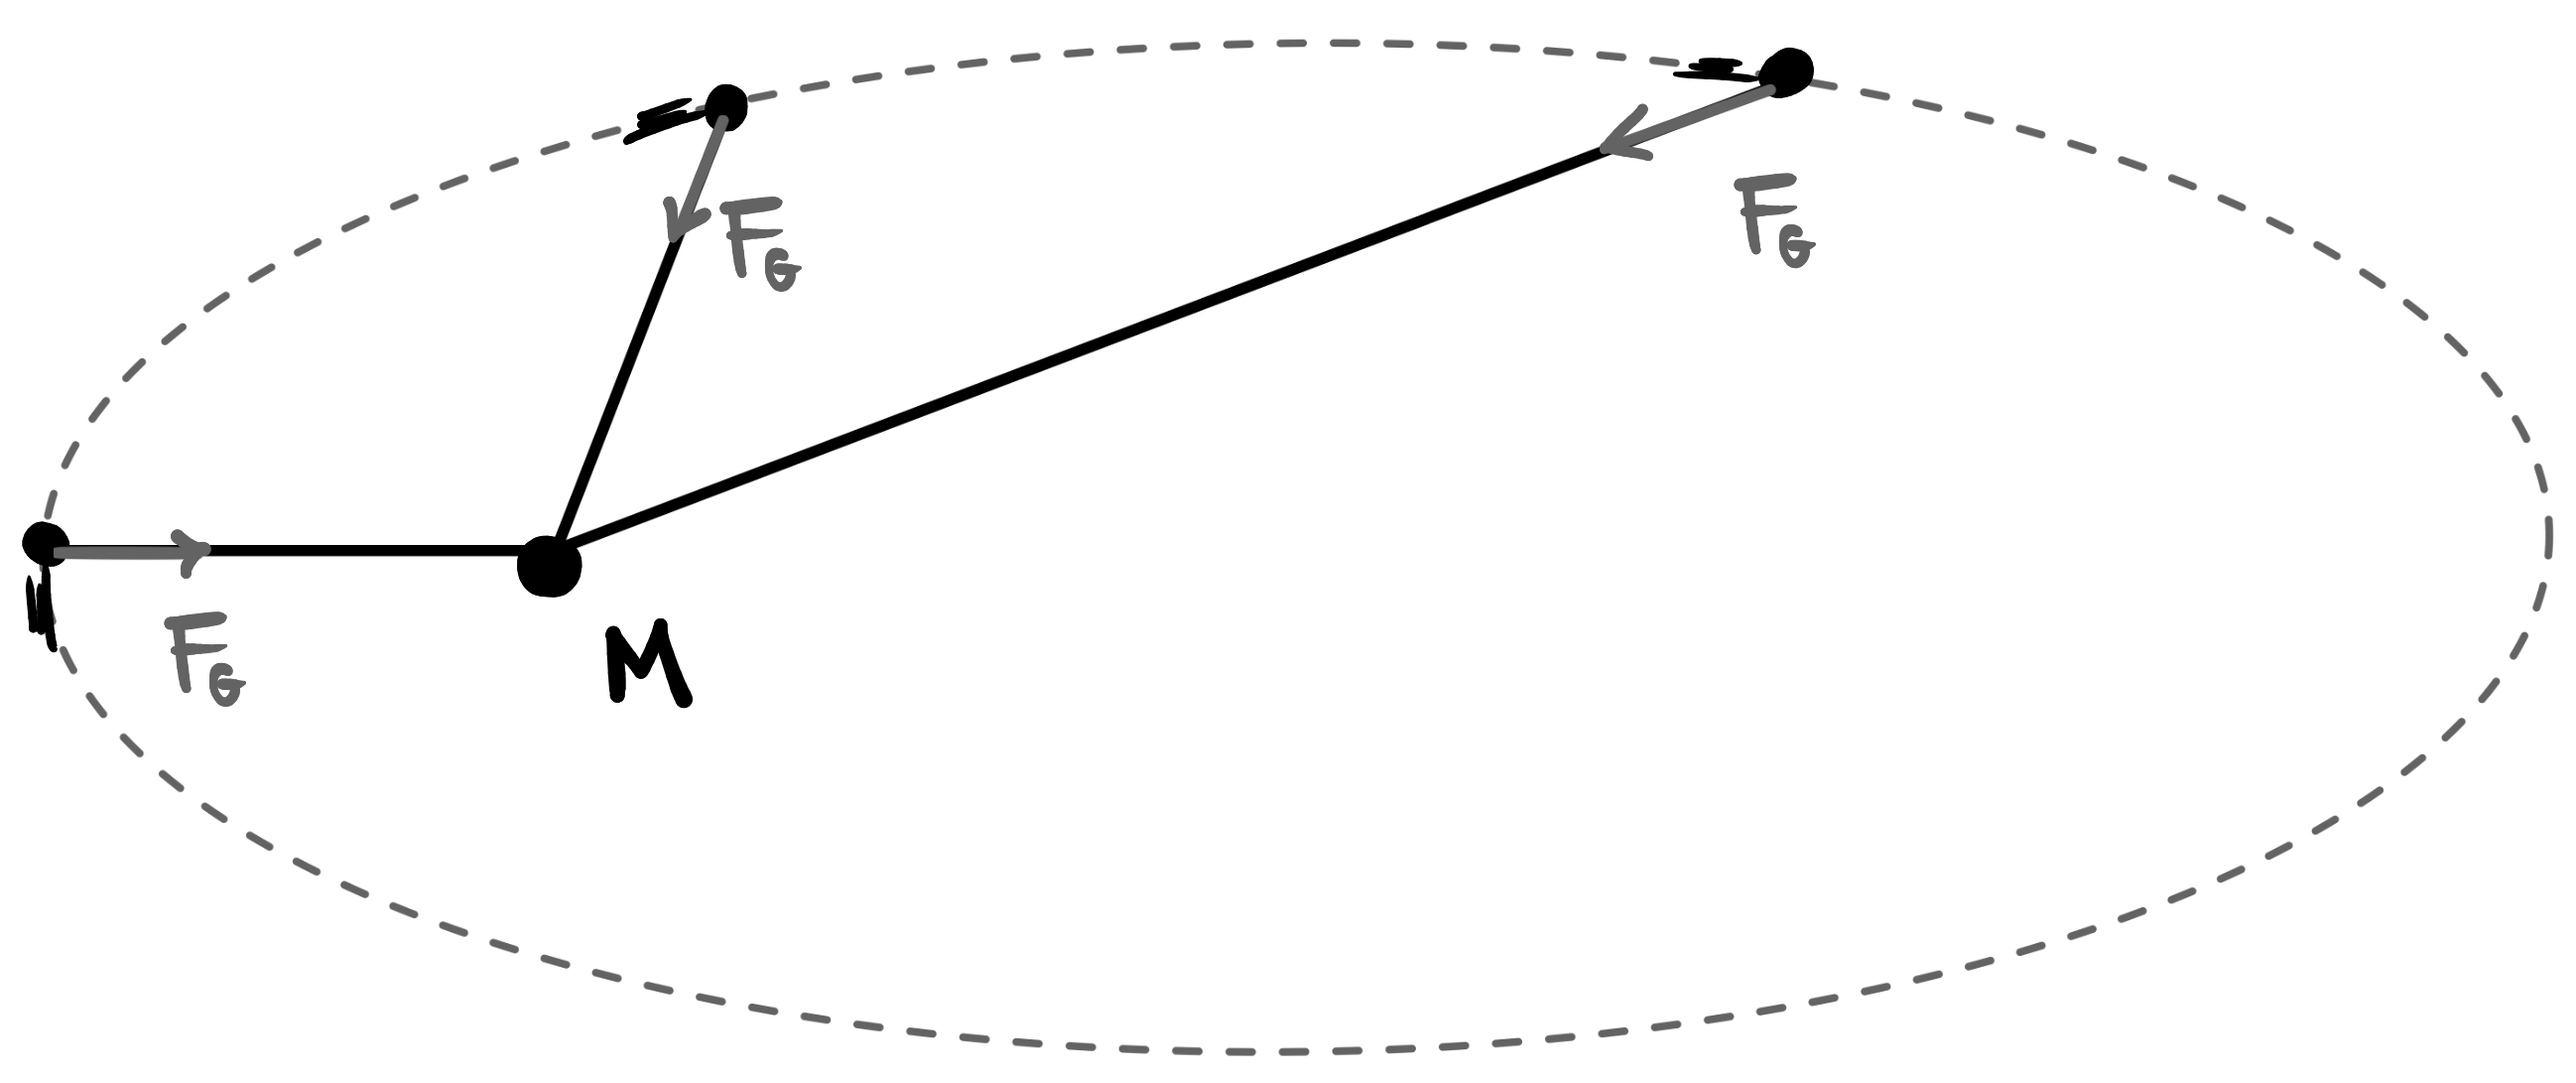
\includegraphics[width=0.6\linewidth]{imagensgravitacao/momentoangularforcacentral.png}};
  \end{scope}
\end{tikzpicture}
\captionof{figure}{O vetor momento angular $\vec L.$}
\label{fig_gravitacao_forcacentral}
} 
\vspace{0.3cm}

Imagine que o satélite em órbita está preso, por uma haste, ao planeta ao redor do qual ele está orbitando. Neste caso, a força gravitacional -- que sempre aponta na direção que une os planetas -- será sempre paralela à haste, de modo que $F_\perp = 0$, isto é, a componente da força perpendicular à barra (que é a componente responsável por gerar torque) é nula, e, portanto, pela Equação \eqref{eq_newton_torque}, seu torque é nulo.

Este é um fato geral: sempre que um corpo está sob a ação de uma força central (e a gravidade é uma força desse tipo)\footnote{Uma força é central quando, em qualquer posição do objeto, ela aponta diretamente para um ponto fixo (que seria o ``centro'') ou diretamente para longe dele.} o torque resultante é nulo e a momento angular, portanto, se conserva.

\secgfe{Erros comuns}

O erro mais comum é o estudante esquecer do termo $\sin \theta$ na Equação \eqref{eq_momento_angular}. Em muitos casos a velocidade $\vec v$ será perpendicular ao vetor posição $\vec r$, de modo que o ângulo $\theta$ será reto, fazendo com que seu seno seja a unidade. Assim, em vários contextos a equação se reduzirá a $L= mvr=pr,$ que representa de fato um ``momento linear'' rotacional, haja vista que estamos apenas multiplicando o momento linear $p=mv$ pelo raio de rotação $r.$

Contudo, é importante notar que o cálculo do momento angular não é este, de modo geral. Deve-se usar a Equação \eqref{eq_momento_angular} e sempre levar em conta o ângulo $\theta$ entre a velocidade $\vec v$ da partícula e o seu vetor posição $\vec r.$

\secgfe{Observações}

O momento angular é, na verdade, uma grandeza vetorial. Tal vetor é sempre perpendicular ao vetor velocidade e ao vetor posição da partícula, de modo que ele é perpendicular ao plano de movimento da partícula,\footnote{Quando tomamos como referência para os torques um ponto que está contido no plano de movimento.} como mostra a Figura \ref{fig_gravitacao_vetorL}.

\vspace{0.3cm}
{
\centering
\begin{tikzpicture}
  \begin{scope}[blend mode=multiply]
    \node {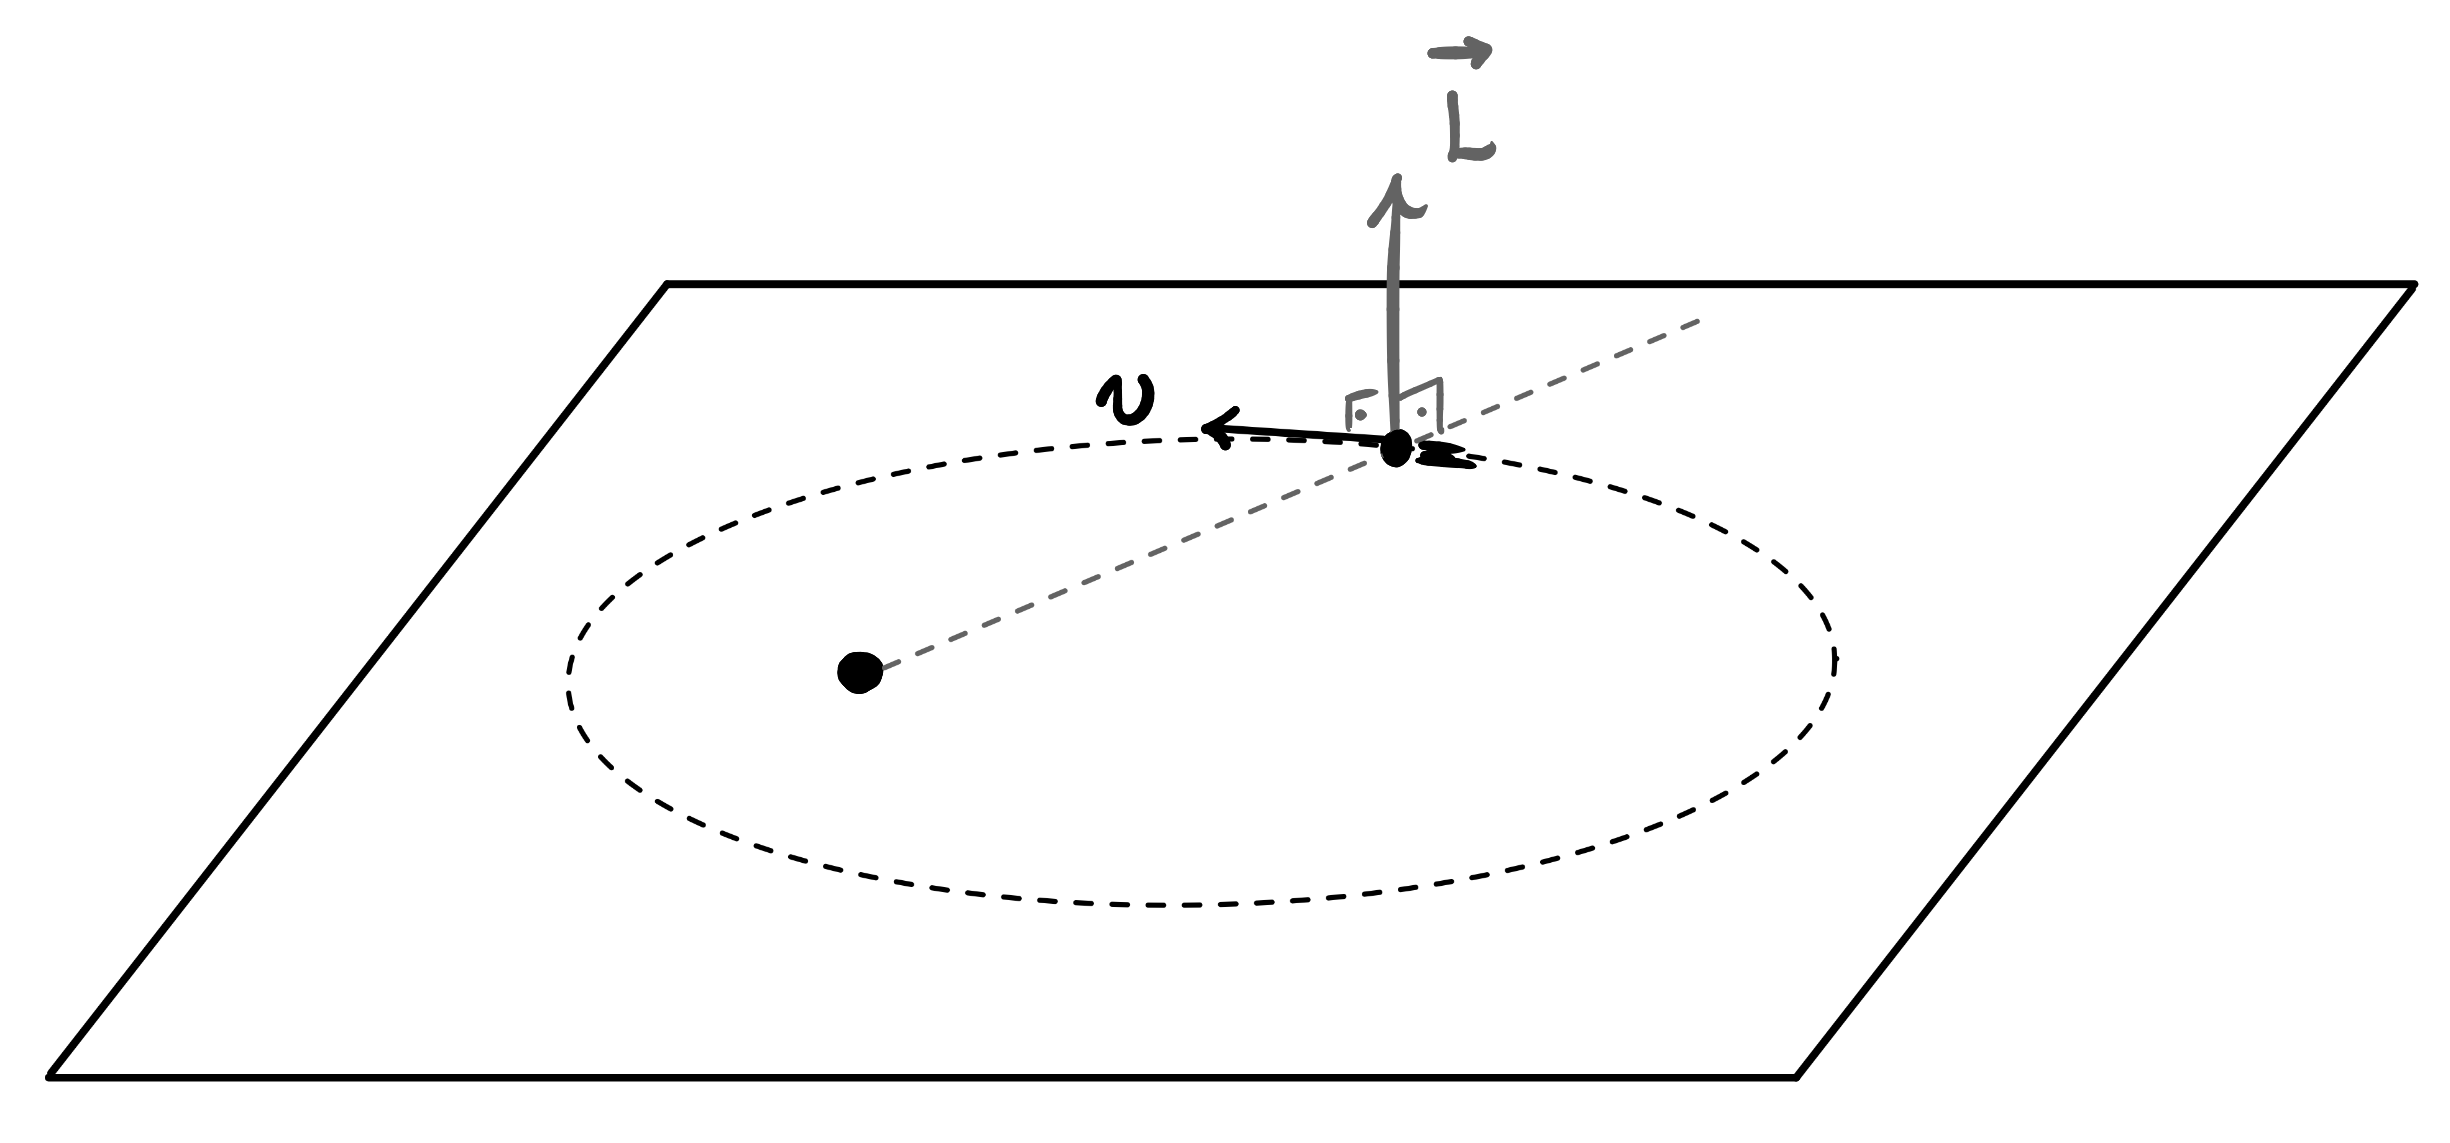
\includegraphics[width=0.5\linewidth]{imagensgravitacao/momentoangularvetor.png}};
  \end{scope}
\end{tikzpicture}
\captionof{figure}{O vetor momento angular $\vec L.$}
\label{fig_gravitacao_vetorL}
} 
\vspace{0.3cm}

Contudo, o seu caráter vetorial pode ser deixado de lado em um primeiro momento, haja vista que, para ser obtido, exigiria o conhecimento da operação de multiplicação de vetores, tema que foge do escopo do livro\footnote{O próprio torque $\tau$ também é, em sua natureza, um vetor, mas suprimos seu caráter vetorial na discussão deste livro.}.


\vspace{0.3cm}

\begin{exemplo}[Nível III]\label{exemplo_rotacao_momentoangularex01}



Uma partícula de massa $m$ move-se em trajetória circular de raio $r$ com velocidade $v$. Em certo instante, o raio da trajetória é reduzido lentamente até $r/2$, sem aplicação de torque externo.

Determine a nova velocidade da partícula.

\resolucao

Como não há torque externo, o momento angular da partícula em relação ao centro da trajetória conserva-se. Inicialmente, tem-se

\[
L_i = mrv.
\]


Ao final do processo, o raio passa a ser $r_f = \sfrac{r}{2}.$ Seja $v_f$ a nova velocidade da partícula. Então,

\[
L_f = m\left(\frac{r}{2}\right)v_f.
\]


Como $L_i=L_f$, segue que

\[
mrv = m\left(\frac{r}{2}\right)v_f.
\]


Logo,

\[
\boxed{v_f = 2v.}
\]







\end{exemplo}


\vspace{0.3cm}



\begin{exemplo}[Nível III]\label{exemplo_rotacao_momentoangularex02}

Prove, a partir da segunda lei de Kepler, que o momento angular é uma grandeza conservada em uma órbita sob ação da força gravitacional.

\resolucao

A segunda lei de Kepler diz que, se um satélite está orbitando um certo planeta de massa $M,$ como mostra a Figura \ref{fig_gravitacao_2ndkeplerslaw}, a linha imaginária que une o satélite ao planeta varre áreas iguais em tempos iguais.



\vspace{0.3cm}
{
\centering
\begin{tikzpicture}
  \begin{scope}[blend mode=multiply]
    \node {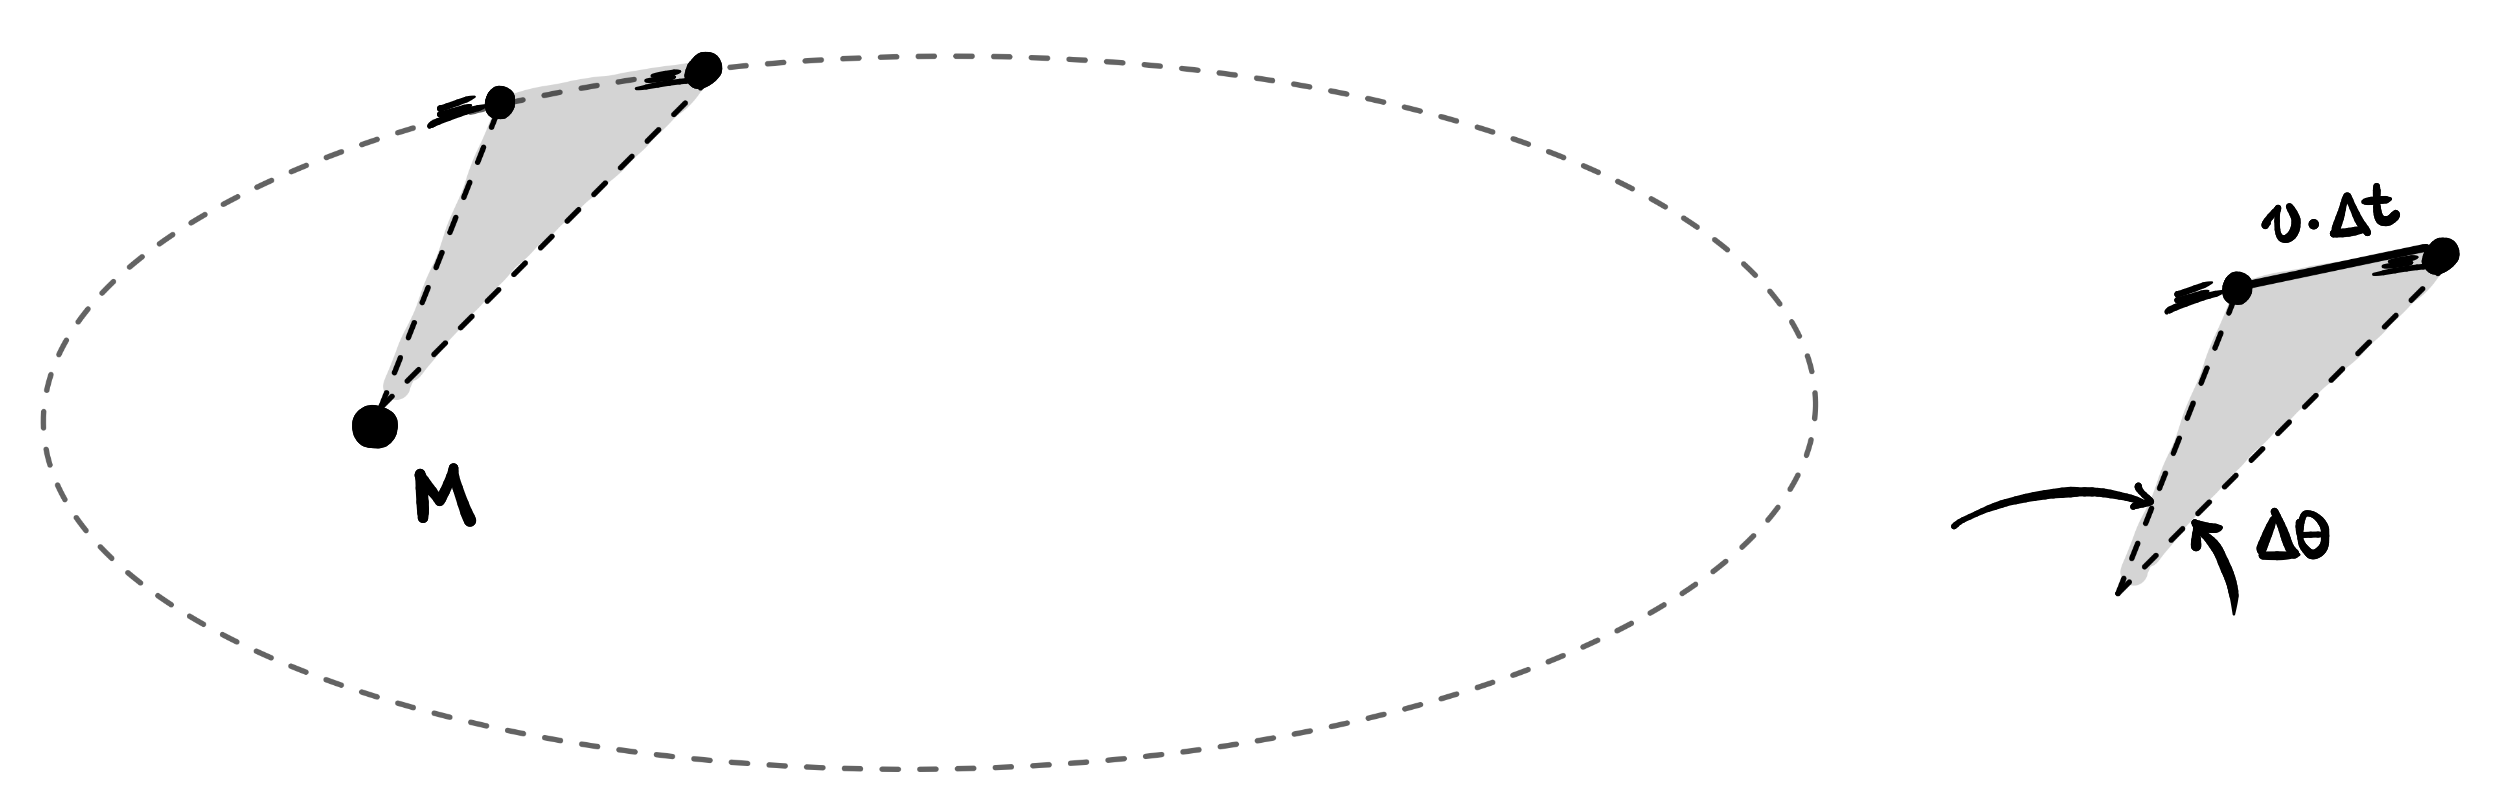
\includegraphics[width=0.7\linewidth]{imagensgravitacao/momentoangularsegundaleikepler.png}};
  \end{scope}
\end{tikzpicture}
\captionof{figure}{A segunda lei de Kepler, matematicamente, é equivalente à conservação do módulo do momento angular.}
\label{fig_gravitacao_2ndkeplerslaw}
} 
\vspace{0.3cm}

Considere dois instantes do movimento do satélite, separados pelo intervalo temporal $\Delta t.$ A distância que o satélite percorre entre um instante e outro é $d=v \Delta t$. Sendo $\Delta \theta$ o deslocamento angular entre tais posições, teremos que a área varrida pelo vetor posição $\vec r$ foi de\footnote{Estamos assumindo que o triângulo em questão é isósceles de lados iguais a $r$, haja vista que, para um intervalo de tempo pequeno $\Delta t$, o lado de tamanho $v\Delta t$ é bem pequeno, de modo que os dois outros lados diferem de um valor infinitesimal.}

$$ A = \dfrac{ab \sin \theta}{2} = \dfrac{r\cdot r \cdot \sin (\Delta \theta)}{2} \approx \dfrac{r^2 \Delta \theta}{2} = \dfrac{r^2}{2} \cdot \dfrac{v\Delta t}{r} = \dfrac{vr \Delta t}{2}.$$


Aqui usamos o fato de que o ângulo $\Delta \theta$ é muito pequeno,\footnote{Partimos dessa premissa quando afirmamos que a distância percorrida entre os dois pontos é dada por $d=v \Delta t$. Isso só valeria se a velocidade fosse constante, o que é uma verdade caso o intervalo de tempo (e consequentemente o ângulo de abertura $\Delta \theta$) entre as duas posições seja tão curto de modo que praticamente não houve tempo da velocidade variar.}, de modo que vale a aproximação para ângulos pequenos $\sin x \approx x,$ para $x$ em radianos. Na sequência usamos a definição de tal ângulo em radianos: ele é a razão entre o comprimento do arco de circunferência que ele enxerga pelo raio de curvatura, isto é, $\Delta \theta = \sfrac{v\Delta t}{r}$.

Assim, dividindo os dois membros da equação por $\Delta t,$ chegamos em

$$ \dfrac{A}{\Delta t} = \dfrac{mvr}{2m} = \dfrac{L}{2m}.$$

Note que a segunda lei de Kepler afirma que o lado esquerdo da equação acima é constante: a velocidade areolar $v_A=\sfrac{A}{\Delta t}$ com que a linha imaginária que une o planeta ao satélite varre áreas é constante. Ou, em outras palavras, ela varre áreas iguais em tempos iguais. Assim, o lado direito da equação também deve sê-lo, de modo que conclui-se que o momento angular $L$ do satélite em órbita é constante.

É possível, portanto, demonstrar a conservação do momento angular usando a segunda lei de Kepler -- esta é, na verdade, a própria lei de conservação do momento angular, porém expressa de um modo em que isso não é tão evidente.

\end{exemplo}



\vspace{0.3cm}














